% Options for packages loaded elsewhere
\PassOptionsToPackage{unicode}{hyperref}
\PassOptionsToPackage{hyphens}{url}
%
\documentclass[
  11pt,
]{article}
\usepackage{amsmath,amssymb}
\usepackage{amsthm}
\providecommand{\llbracket}{\mathopen{[\![}}
\providecommand{\rrbracket}{\mathclose{]\!]}}
\usepackage{iftex}
\ifPDFTeX
  \usepackage[T1]{fontenc}
  \usepackage[utf8]{inputenc}
  \usepackage{textcomp} % provide euro and other symbols
\else % if luatex or xetex
  \usepackage{unicode-math} % this also loads fontspec
  \defaultfontfeatures{Scale=MatchLowercase}
  \defaultfontfeatures[\rmfamily]{Ligatures=TeX,Scale=1}
\fi
\usepackage{newunicodechar}
\newunicodechar{⇒}{\ensuremath{\Rightarrow}}
\newunicodechar{⇔}{\ensuremath{\Leftrightarrow}}
\newunicodechar{↔}{\ensuremath{\leftrightarrow}}
\ifPDFTeX\else
  \newunicodechar{→}{\ensuremath{\to}}
\fi
\usepackage{lmodern}
\ifPDFTeX\else
  % xetex/luatex font selection
\fi
% Use upquote if available, for straight quotes in verbatim environments
\IfFileExists{upquote.sty}{\usepackage{upquote}}{}
\IfFileExists{microtype.sty}{% use microtype if available
  \usepackage[]{microtype}
  \UseMicrotypeSet[protrusion]{basicmath} % disable protrusion for tt fonts
}{}
\makeatletter
\@ifundefined{KOMAClassName}{% if non-KOMA class
  \IfFileExists{parskip.sty}{%
    \usepackage{parskip}
  }{% else
    \setlength{\parindent}{0pt}
    \setlength{\parskip}{6pt plus 2pt minus 1pt}}
}{% if KOMA class
  \KOMAoptions{parskip=half}}
\makeatother
\usepackage{xcolor}
\usepackage{graphicx}
\usepackage{longtable,booktabs,array}
\usepackage{calc} % for calculating minipage widths
\usepackage{placeins}
\usepackage{tikz}
\usetikzlibrary{arrows.meta,positioning,shapes.geometric,calc}
\tikzset{
bcbox/.style={rectangle,rounded corners,draw,align=center,inner sep=2.5pt,minimum width=3.2cm,minimum height=0.55cm,text width=3.2cm},
bcwide/.style={rectangle,rounded corners,draw,align=center,inner sep=2.5pt,minimum width=4.05cm,minimum height=0.58cm,text width=4.05cm},
bcdec/.style={diamond,draw,aspect=2.15,align=center,inner sep=1pt,minimum width=3.35cm,text width=2.75cm},
bcterm/.style={ellipse,draw,align=center,inner sep=2.5pt,minimum width=2.85cm,text width=2.85cm},
bccheck/.style={densely dotted},
bcaudit/.style={bcdec,bclemma,bccheck},
bcauditbox/.style={bcdec,bclemma,bccheck},
bcscopefail/.style={rectangle,draw,dashed,red!65!black,fill=red!6,align=center,inner sep=2.5pt,minimum width=2.85cm,text width=2.85cm},
bcclosed/.style={bcterm,fill=green!16},
bcresidual/.style={bcbox},
bcroute/.style={rectangle,rounded corners,draw,fill=yellow!18,align=center,inner sep=2pt,minimum width=2.85cm,text width=2.85cm},
bcroutechoice/.style={diamond,draw,fill=yellow!10,aspect=2.05,align=center,inner sep=1pt,minimum width=2.95cm,text width=2.45cm},
bcroutepanel/.style={rectangle,rounded corners,draw,fill=yellow!10,align=center,inner sep=2.4pt,minimum width=3.55cm,text width=3.55cm},
bcdefinition/.style={fill=blue!12,draw=blue!60!black},
bclemma/.style={fill=purple!12,draw=purple!65!black},
bcproposition/.style={fill=orange!18,draw=orange!75!black},
bccorollary/.style={fill=teal!12,draw=teal!65!black},
bctheorem/.style={fill=red!10,draw=red!60!black},
bcrouteneutral/.style={fill=white,draw=orange!70!black},
bcdesign/.style={dashed},
bcpayload/.style={thick},
bcarr/.style={-{Latex[length=2mm]},thick,shorten <=1.5pt,shorten >=1.5pt},
bcloop/.style={bcarr},
bchandoff/.style={-{Latex[length=2mm]},thick,densely dotted,shorten <=1.5pt,shorten >=1.5pt},
bccheckarr/.style={bchandoff},
bcrecoverarr/.style={-{Latex[length=2mm]},thick,dashed,shorten <=1.5pt,shorten >=1.5pt},
bcscopearr/.style={-{Latex[length=2mm]},thick,dashed,red!65!black,shorten <=1.5pt,shorten >=1.5pt},
bcoutputroute/.style={densely dotted},
bclabel/.style={font=\scriptsize,inner sep=1.4pt,fill=white}
}
% Correct order of tables after \paragraph or \subparagraph
\usepackage{etoolbox}
\makeatletter
\patchcmd\longtable{\par}{\if@noskipsec\mbox{}\fi\par}{}{}
\makeatother
% Allow footnotes in longtable head/foot
\IfFileExists{footnotehyper.sty}{\usepackage{footnotehyper}}{\usepackage{footnote}}
\makesavenoteenv{longtable}
\setlength{\emergencystretch}{3em} % prevent overfull lines
\providecommand{\tightlist}{%
  \setlength{\itemsep}{0pt}\setlength{\parskip}{0pt}}
\setcounter{tocdepth}{2}
\setcounter{secnumdepth}{2}
\theoremstyle{definition}
\newtheorem{definition}{Definition}[section]
\newtheorem{example}{Example}[section]
\newtheorem{lemmaschema}{Lemma schema}[section]
\newtheorem{algorithm}{Algorithm}
\ifLuaTeX
  \usepackage{selnolig}  % disable illegal ligatures
\fi
\usepackage[]{natbib}
\usepackage{bookmark}
\IfFileExists{xurl.sty}{\usepackage{xurl}}{} % add URL line breaks if available
\urlstyle{same}
\hypersetup{
  hidelinks,
  pdfcreator={LaTeX},
  pdftitle={Structural Exhaustion: A Reference Manual for AI-Assisted Theorem Proving},
  pdfauthor={Guillem Duran-Ballester},
  pdfsubject={Auditable human-supervised LLM-assisted theorem proving},
  pdfkeywords={AI-assisted theorem proving, structural exhaustion, minimal counterexample, proof auditing}}
\newcommand{\secref}[1]{\hyperref[#1]{Section~\ref*{#1}}}
\newcommand{\secrange}[2]{\hyperref[#1]{Sections~\ref*{#1}}--\hyperref[#2]{\ref*{#2}}}
\newcommand{\appref}[1]{\hyperref[#1]{Appendix~\ref*{#1}}}
\newcommand{\scoperef}{\hyperref[the-scope-condition-locally-testable-targets]{scope}}
\newcommand{\sectextref}[2]{\hyperref[#2]{#1}}
\newcommand{\ctsignature}[1]{\par\noindent\emph{Signature.}\ #1\par\medskip}
\newcommand{\ctcert}[1]{\mathrm{Cert}\{#1\}}
\newcommand{\ctint}[1]{\mathrm{Int}\{#1\}}
\newcommand{\ctrec}[1]{\mathrm{Rec}\{#1\}}
\newcommand{\ctnone}{\varnothing}
\newcommand{\ctpar}[1]{\paragraph{#1.}}

\title{Structural Exhaustion\\[0.4em]
\large A Reference Manual for AI-Assisted Theorem Proving via Structural
Bookkeeping and Textbook Combinatorial Methods}
\author{Guillem Duran-Ballester}
\date{July 7, 2026}

\begin{document}

\maketitle

\begin{abstract}
Long AI-assisted proofs are difficult to inspect when case choices, residual
obligations, and uses of quantitative slack remain implicit. This document
specifies \emph{structural exhaustion}, a reference manual for human-supervised,
LLM-assisted development and review of structural-exhaustion and
minimal-counterexample arguments. It is intended for extremal and
combinatorial proofs that can be organized through explicit case splits, local
reductions, finite-state reasoning, and quantitative budgets. The manual
supplies three coordinated components: a typed library of proof tactics, a
strategy manual for selecting and parameterizing them, and an assurance layer
for auditing their inputs, outputs, and dependencies. A candidate proof is
represented by finitely recorded branch states containing its standing
hypotheses, certified exclusions on the current branch path, residual
conditions, and target-relevant interface data. An instantiation is complete only when every terminal branch
returns one of the five declared certificate classes and every nonterminal
residual has a declared downstream consumer. Capacity closures combine local
accounting inequalities. The remaining terminal classes cover direct target
realization, minimality or compression, routed defect accounts, and finite
enumeration.
These are protocol requirements rather than a guarantee of automated
discovery: the LLM proposes steps within the declared state system, while human
reviewers verify the local mathematics, routing contracts, and terminal
certificates. The Erdős--Gyárfás
power-of-two-cycle instantiation provides the full-scale proof model
motivating this architecture.
\end{abstract}

\paragraph*{AI-use disclosure.}
AI tools were used as drafting and proof-engineering aids. The author
reviewed all outputs and is responsible for all mathematical and
methodological claims; model output is not used as evidence of
correctness.

\tableofcontents

\section*{Introduction}\label{introduction}

In 1977, Appel and Haken, with Koch, proved the Four-Colour Theorem using
reducibility, discharging, and computational verification
\citep{appel-haken-1977-discharging,appel-haken-koch-1977-reducibility}.
Their proof remains a useful reference point for methodologies that
replace a compact global argument by an explicit family of local
obligations. The present manual studies a related proof-engineering
trade-off in AI-assisted combinatorial theorem proving.

The cost profile of proof engineering has changed with contemporary
language-model tools. This manual adopts a conservative operating
assumption: model output is not treated as an autonomous source of global
mathematical conclusions. Within a constrained interface, a model can
instead maintain structured state, expand local cases, enforce fixed
formats, and draft repetitive derivations for human review. Structural
exhaustion formalizes that interface as a transition system over branch
states, typed residuals, local certificates, finite labels, ledgers,
budgets, and dependency records.

The architecture is designed against a declared threat model for
LLM-assisted proof development. A generated draft may omit the step that
carries the difficulty, use a global estimate with an unrecorded
independence assumption or double count, restate the original problem as
an auxiliary lemma, supply unsupported proof-shaped prose, or accept an
incorrect proposed step. These are design risks that the protocol is
intended to expose, not empirical claims that every model or proof task
exhibits them uniformly. The manual therefore requires local obligations,
typed residuals, and checkable certificates at the proof interface.

Stronger models, formal verification, formal-first development,
interactive theorem proving, retrieval, and human review can all improve
reliability. Structural exhaustion addresses the complementary question
of how a proof is developed before final verification: it decomposes
proof search into constrained local obligations whose outputs are typed,
routed, and audited.

The framework is based on the following organizing principle. A putative
counterexample can avoid the target only by spending some scarce
resource, violating an accumulated exclusion, or creating a repeatable
local operation. Scarce resources are charged by ledgers and budgets.
Exclusions are recorded in the branch state and spent by dichotomies.
Repetitions are consumed by pumping, exchange, exact typing, or
compression. The proof does not ask for an unstructured global insight;
it maintains these accounts until a branch produces a certificate or a
typed residual routed to a downstream closure tactic.

The machinery converts a minimal-counterexample argument into the
maintenance of explicit data structures: branch states that accumulate
every standing hypothesis and every prior exclusion, external types
recording what a bounded piece can exhibit to its surroundings, ledgers
routing demands to scarce payers, budgets in a fixed normal form, and
typed payloads passing between proof steps. These data evolve under a
fixed transition system of seventeen
\textbf{closure tactics} whose moves are textbook: minimality and
replacement, charging, exchange, pigeonhole, finite-state repetition,
compression, and finite enumeration. A completed instantiation is
leaf-total. Every terminal branch must end in one of the five certificate
classes C1--C5. A residual is not a final state; it is a typed payload
with a declared consumer in the interlock graph. If a branch emits a
residual with no consumer, the proof has not reached an open
mathematical leaf --- it has failed to compile. Every step either closes
a branch or emits a strictly smaller, explicitly typed residual, so an
omitted step is not a stylistic lapse but a syntactic violation, visible
before any mathematical judgment is required. Global estimates are
admitted only after their hypotheses and accounting steps have been
decomposed into named, auditable premises. Capacity inequalities are one
recurring output of that decomposition.

The manual separates mechanism, policy, and verification.
\secref{motivation-and-literature-background} motivates the architecture;
\secref{part-ii-the-tactic-library} defines the proof language, tactic
interfaces, and local obligations; \secref{part-iii-the-strategy-manual}
governs admission, parameter synthesis, selection, and sequencing; and
\secref{part-iv-assurance} supplies the audit artifacts and failure
semantics. The interfaces make the obligations explicit and checkable;
proving an instance-specific obligation may still require substantial
mathematical judgment.

Two properties distinguish the resulting proofs from conventional long
arguments, and both are consequences of the no-unnamed-residuals
discipline. The first is graceful degradation. Because every branch
failure produces a named, typed residual class, the retraction of any
closing lemma does not collapse the proof; it relocates the conclusion
to an explicit reduction theorem, with a computable blast radius.
Partial verification is therefore not partial confidence: a reader who
has checked some of the branches has unconditionally established the
corresponding reduction theorem, and further checking only moves the
result up a lattice whose top is the unconditional statement. The second
is a three-label audit taxonomy. This taxonomy is an operational policy,
not a theorem that every objection falls immediately and uniquely into
one class. An apparent non-closure is recorded as an execution error only
when a required obligation is absent or invalid, as a design failure only
when a typed obstruction has a declared repair route, and as a scope
obstruction only after the language-extension audit has established
nonexpressibility in the current proof language. The base language is
designed for targets represented by finite local tests and finite type
data under bounded-interface gluing. The spectral-gap discussion in the
\sectextref{limitations section}{limitations} is a proposed example of
extending that language with cut and energy descriptors, not a claim that
every spectral argument is thereby admitted.

The primary case study is the companion candidate manuscript
\emph{A Structural Exhaustion Proof of the Erd\H{o}s--Gy\'arf\'as
Power-of-Two Cycle Problem} \citep{duran-ballester-2026-eg-candidate},
hereafter \textup{[EG]}. The release package contains its source as
\texttt{../erdos\_64\_proof.tex} and its live review dossier as
\texttt{../erdos\_64\_proof\_review.md}. The dossier records known
defects, repairs, and open review obligations; accordingly, [EG] is
presented as a candidate proof under public review rather than as an
independently verified result. The appendix maps this manual to [EG], and
\appref{appendix-c.-a-small-worked-instantiation} gives a smaller worked
example. Readers are invited to check the companion's named interfaces,
computations, and unresolved routes and to contribute corrections or
repairs.

\begingroup
\small
\setlength{\tabcolsep}{2pt}
\begin{longtable}[]{@{}
  >{\raggedright\arraybackslash}p{0.20\linewidth}
  >{\raggedright\arraybackslash}p{0.30\linewidth}
  >{\raggedright\arraybackslash}p{0.42\linewidth}@{}}
\caption{Rosetta table for the main structural-exhaustion vocabulary.}
\label{tab:introduction-rosetta}\\
\toprule\noalign{}
Framework term & Classical neighbour & What the framework adds \\
\midrule\noalign{}
\endfirsthead
\toprule\noalign{}
Framework term & Classical neighbour & What the framework adds \\
\midrule\noalign{}
\endhead
\bottomrule\noalign{}
\endlastfoot
Branch state & Case with hypotheses & The full accumulated context:
baseline assumptions, minimality, certified exclusions accumulated along
the current branch path, invariants,
residual condition, and queued payloads. \\
Local test & Local witness or obstruction & A bounded family whose
realization is equivalent to the target inside the declared scope. \\
External type & Myhill--Nerode-style context equivalence; logical type & A live proof
coordinate deciding exits, neutral exchanges, replacement, and typed
handoffs. \\
Ledger & Charging or discharging account & Canonical demands, payers,
capacities, tie-breaking, and bounded multiplicity as auditable data. \\
Budget & Potential function & A normal-form quantitative account with
recorded currencies, additivity, monotonicity, and slack. \\
Payload & Intermediate lemma conclusion & A typed tuple whose producer
and consumer are both recorded, so every non-closing exit has a declared
route. \\
Closure tactic & Standard proof move & A fixed mechanism interface
returning only a certificate C1--C5 or a named residual payload. \\
Residual & Remaining subcase & A fully typed branch state that can stand
alone as a reduction theorem if its closure later fails. \\
\end{longtable}
\endgroup

\section{Motivation and design rationale}\label{motivation-and-literature-background}

The method targets theorems of the shape

\[
\begin{gathered}
\text{every object satisfying baseline hypotheses}\\
\text{contains a specified target configuration.}
\end{gathered}
\]

One assumes a minimal counterexample and converts the proof into a
controlled elimination of every way it could avoid the target.

\subsection{The core pattern}\label{the-core-pattern}

The strategy has five recurring layers:

\[
\boxed{
\begin{gathered}
\text{minimal counterexample}
\;\Rightarrow\;
\text{local state space}
\;\Rightarrow\;
\text{branch split}\\
\Rightarrow\;
\text{charging / compression / finite routing}
\;\Rightarrow\;
\text{contradiction}.
\end{gathered}
}
\]



The essential discipline is that \textbf{every branch is an explicit
state}. The logical core of the formal branch-state tuple records the
accumulated context of a case: to say ``we are in branch \(B\)'' includes

\[
\begin{aligned}
B \;={}& \text{baseline hypotheses} \;+\; \text{minimality}\\
&+ \text{certified exclusions on the current branch path}\\
&+ \text{current residual condition}.
\end{aligned}
\]

This prevents a pervasive error in case-based arguments: treating a
residual as if it were unconstrained. In this method, every residual
carries the full history of constraints under which it arose. The full
eight-component state is defined in \secref{data-branch-states}.

\subsection{Literature positioning}\label{literature-positioning}

The method packages standard proof moves into an explicit branch-closure
architecture. Its primitive moves are inherited from
minimal-counterexample arguments, discharging, finite-state repetition,
and replacement. The closest predecessors are the discharging and
reducibility tradition around the four-colour theorem, especially the
work of Appel--Haken and the later Robertson--Sanders--Seymour--Thomas
proof
\citep{appel-haken-1977-discharging, appel-haken-koch-1977-reducibility, robertson-etal-1996-new-proof, robertson-etal-1997-four-colour}.
Cranston--West serves as a general survey of discharging as a reusable
method \citep{cranston-west-2017-discharging}. Those sources are the
right comparison point whenever the present document speaks about local
reducibility, finite certified leaves, unavoidable local configurations,
or charging/discharging arguments. In the classical proofs, the
reducible configurations, discharging rules, and potential-like
quantities enter through problem-specific insight. In the present
framework, the same kinds of objects become branch-state data generated
from the resource inventory, the both-sides test, and the budget
checklist, so several interacting charges and invariants can be
maintained simultaneously.

The second comparison point is the finite-state and context-equivalence
literature. The external-type language below is deliberately
Myhill--Nerode-like: two pieces have the same type when no compatible
context can separate them with respect to the target
\citep{myhill-1957-automata, nerode-1958-linear}. In graph and logic
settings this viewpoint is aligned with Courcelle's monadic second-order
treatment of graph properties and with Courcelle--Engelfriet's
language-theoretic account of graph structure
\citep{courcelle-1990-mso-graphs, courcelle-engelfriet-2012-graph-structure}.
In those settings, types commonly support recognition, automata, or
dynamic programming. Here they also function as live proof coordinates:
an external type records which exits remain available, when an exchange
is neutral, and when replacement/minimality can close a branch.

In parameterized complexity, the closest technical relatives are finite
integer index, boundaried graphs, protrusion replacement, and explicit
representative replacement. The relevant line includes
Bodlaender--Fomin--Lokshtanov--Penninkx--Saurabh--Thilikos and
subsequent work of Kim and coauthors, Garnero and coauthors, and
Jansen--Wulms
\citep{bodlaender-etal-2009-meta-kernelization, kim-etal-2012-protrusion, garnero-etal-2013-explicit-kernels, jansen-wulms-2016-lower-bounds}.
That literature supplies representative sets and replacement relations
for algorithmic reduction. The present framework uses the same
finite-interface discipline as a routing language inside a contradiction
proof: representatives, carrier quotients, and exact types are generated
as needed by the branch state and then consumed by compression, defect,
or handoff routes.

The Erdős--Gyárfás power-of-two-cycle instantiation places the method in
the cycle-length forcing literature around the Erdős--Gyárfás
power-of-two cycle problem. The
relevant background includes the classical even-cycle extremal theorem
of Bondy--Simonovits, the sparse cycle-length results of
Sudakov--Verstraete, and the recent class-restricted progress for
\(P_8\)-free, \(P_{10}\)-free, and \(P_{13}\)-free graphs by Gao--Shan,
Hu--Shen, and Hegde--Sandeep--Shashank, respectively
\citep{bondy-simonovits-1974-even-cycles, sudakov-verstraete-2008-cycle-lengths, gao-shan-2021-p8, hu-shen-2023-p10, hegde-etal-2024-p13}.
Carr's 2026 structural result is especially relevant because it also
studies minimal counterexamples to the Erdős--Gyárfás conjecture
\citep{carr-2026-minimal-counterexample}. The
comparison here is methodological: the cycle-length literature provides
problem-specific structural insight, while the branch-closure framework
specifies how local tests, first-failure witnesses, target thickenings,
and budget rates are produced and sequenced inside a single auditable
state system.

Finally, the machine-assistance design discipline belongs beside the
recent literature on autoformalization and proof-search scaffolding. The
closest anchors are Wu et al.~on autoformalization, Jiang et al.~on
Draft--Sketch--Prove, and Yang et al.~on LeanDojo
\citep{wu-etal-2022-autoformalization, jiang-etal-2022-draft-sketch-prove, yang-etal-2023-leandojo}.
The present document functions as a proof-architecture discipline: its
point of contact with that literature is the shared need to decompose
long arguments into explicit local obligations with recorded
dependencies. The distinction is that the present framework organizes
the informal combinatorial construction before formalization: it
generates ledger entries, invariant registers, handoff payloads, and
closure certificates that can later be checked by a human or a formal
system.

The contribution is a reference architecture rather than a new primitive
combinatorial move. Its concrete components are a typed proof-language
specification, seventeen tactic contracts, a registered payload-routing
system, strategy and repair procedures, an [EG] crosswalk, and a complete
small worked example. Together these components record which hypotheses,
invariants, quantitative accounts, and residual routes support each
closure step.

\subsection{Design rationale: AI-assisted theorem
proving}\label{design-rationale-scaffolding-for-llm-assisted-proof-development}

Beyond its mathematical content, structural exhaustion is engineered as
a framework for AI-assisted theorem proving. It assigns language models
structured tasks such as maintaining state, proposing case splits,
filling ledgers, generating local tests, and drafting named obligations
inside a fixed audit format. It shares with
autoformalization, proof-sketch-guided proving, and retrieval-augmented
formal proving the premise that long arguments become tractable when
decomposed into explicit local obligations with visible dependencies
\citep{wu-etal-2022-autoformalization, jiang-etal-2022-draft-sketch-prove, yang-etal-2023-leandojo}.
The following seven items are operational risks observed while developing
[EG] and are treated here as design assumptions. They are not claims
about the frequency of these behaviours across all models or proof
tasks. The method turns each risk into a structural check.

\textbf{Failure mode 1: omitted difficult steps.} A generated draft may
read like a proof while omitting the step that carries the difficulty.
The countermeasure is the closure discipline of
\secref{closure-criteria-and-the-branch-table} and
\secref{structural-invariants-of-the-method}. A branch closes when every leaf
terminates in one of a fixed, finite list of certificate types, and
every residual has a name. Phrases such as ``this structure should be
impossible'' or ``this cannot happen generically'' are classified as
\emph{prompts for further stratification}. The enumerated terminal
states expose an omitted step syntactically, before any mathematical
judgment is required.

\textbf{Failure mode 2: unsupported global estimates.} An unconstrained
draft may gravitate toward a single global inequality --- a
counting argument, an entropy bound, a spectral estimate --- that
appears to resolve everything at once. Such estimates concentrate the
common errors: an unjustified independence assumption, a double count,
or a boundary term absorbed without justification.

In the simplest unweighted case, the template admits a statement of the
form \(|\mathcal D|\le C\,|\mathcal P|\), obtained from a canonical
charging scheme and a bounded-multiplicity lemma
(\secref{charging-schemes}). The weighted and payer-specific form is the
ledger inequality of \secref{data-ledgers}. Each ingredient is a named
local claim, and the global conclusion is the output of that bookkeeping.

\textbf{Failure mode 3: re-encoding the difficulty.} A model that stalls
on a step may request ``one more lemma'' whose statement restates
the original problem at another level. The progress invariant of \secref{closure-criteria-and-the-branch-table} detects this relocation: every step outputs either a closed branch or
a \emph{strictly smaller} named residual --- smaller in size, in the
number of live exits, or in an explicitly monitored complexity
parameter.

A proposed lemma qualifies as progress when its residual is smaller,
finite, charged, or routed. \secref{bookkeeping-versus-new-theorems} supplies the complementary
diagnostic: a bookkeeping step factors through overload, monochromatic
extraction, and the exchange trichotomy; an unconditional statement
about all large objects with some property is a new global theorem
requiring further branch refinement.

\textbf{Failure mode 4: extrapolation beyond standard material.}
The protocol assumes that model-generated steps require closer scrutiny
when an argument leaves well-represented material. The base library
therefore organizes a small vocabulary of standard mechanisms:
minimal-counterexample replacement, charging
arguments with bounded multiplicity, pigeonhole and finite-state
repetition, matching and star extraction, exchange arguments, and
exhaustive finite enumeration. Instance-specific lemmas, imported
results, and proof-language extensions remain separate audited
obligations; membership in the library does not make their proofs
automatic.

\textbf{Failure mode 5: untyped residuals.} A model may declare that
the adversarial object has none of the structures required by the
available tools and then treat the remaining case as a reason to stop.
The countermeasure is the branch-state ledger. The absence of a feature
is recorded as a positive fact and routed: it feeds a budget, strengthens
an exclusion, creates a repetition payload, or triggers a level-4
language extension under \secref{the-repair-protocol}. An untyped residual is an invalid
worksheet row, not an open mathematical case.

\textbf{Failure mode 6: deferential agreement with erroneous steps.} A
model in an assistant role may accept a user-supplied step whose
hypotheses, quantifiers, branch state, or output type do not match the
current proof obligation. The failure is not mathematical creativity; it
is loss of interface discipline. The countermeasure is that agreement
has no formal status. A proposed step enters the system only as a
worksheet row with declared inputs, quantitative data, schema
obligations, and a typed output. The schema alphabet is defined in
\secref{data-lemma-schemas}; the row is accepted only after the relevant
definition, dichotomy, composition, routing, trigger, or S-Meas obligation is
discharged. When the row fails, the required response is a typed reject,
a named residual, or an alternative routed payload, not conversational
assent.

\textbf{Failure mode 7: status-cue audit drift.} A model may replace a
local audit by an appeal to a problem's published status. Status is
useful context but is neither a certificate nor a defect. Positive steps
and red-team objections use the same interface: each objection must name
a failed schema, missing import, stale branch state, unconsumed payload,
unregistered global theorem, or candidate scope issue. Inventing a new
terminal such as ``open problem'' or ``untyped residual'' is return-alphabet
drift. Certification remains a property of the documented mathematical,
computational, and review artifacts.

\subsection{The formalization
bridge}\label{the-formalization-bridge}

The artifacts of this framework are designed to admit possible formal
encodings. The table describes intended correspondences rather than a
claim that the encodings have already been implemented. The framework is
\textbf{pre-formal}: it organizes the informal combinatorial construction
into local obligations with recorded dependencies, the same shape
consumed by sketch-guided and retrieval-augmented formal proving
\citep{wu-etal-2022-autoformalization, jiang-etal-2022-draft-sketch-prove, yang-etal-2023-leandojo}.

\begin{longtable}[]{@{}
  >{\raggedright\arraybackslash}p{(\columnwidth - 4\tabcolsep) * \real{0.3333}}
  >{\raggedright\arraybackslash}p{(\columnwidth - 4\tabcolsep) * \real{0.3333}}
  >{\raggedright\arraybackslash}p{(\columnwidth - 4\tabcolsep) * \real{0.3333}}@{}}
\caption{Intended formal encodings of the manual's audit artifacts.}
\\
\toprule\noalign{}
\begin{minipage}[b]{\linewidth}\raggedright
Artifact in this document
\end{minipage} & \begin{minipage}[b]{\linewidth}\raggedright
Formal counterpart
\end{minipage} & \begin{minipage}[b]{\linewidth}\raggedright
Consequence
\end{minipage} \\
\midrule\noalign{}
\endhead
\bottomrule\noalign{}
\endlastfoot
\label{tab:formalization-bridge}
Branch state & The local hypothesis context in a proof assistant;
entering a branch extends the context & Cumulative constraints are
enforced by the kernel rather than by reader memory \\
Invariant register & A named-lemma ledger, one declaration per invariant
& ``Established at stage \(X\), consumed at stage \(Y\)'' becomes import
order \\
Typed handoff & A lemma signature, with the payload as the explicit
argument list & A format mismatch is a type error before proof search
begins \\
Branch table & An exhaustive case split with no wildcard arm & ``No
unnamed residuals'' becomes checked exhaustiveness \\
Closure certificates & Terminal tactics: contradiction, minimality, and
verified computation for finite leaves & The certificate list of \secref{what-counts-as-a-finished-branch} becomes a fixed tactic vocabulary \\
Finite enumerations and published code & Decision procedures or verified
computation & The code appendix becomes a decidable instance rather than
trusted output \\
Peeling loop (\secref{peeling-loops-closure-by-well-founded-recursion}) & Well-founded recursion with an explicit
termination measure & The per-pass peel lemma is the decreasing-measure
obligation \\
Exact external type (\secref{the-whole-object-piece-exact-types-under-context-degeneracy}) & An explicit data structure, with
identification only through a proved equivalence & Quotienting through
the empty context requires a stated equality proof \\
Reverse index (\secref{proof-engineering-artifacts}) & Machine-assisted premise/dependency extraction
over the development & The blast radius of \secref{bounded-blast-radius} is a graph
query \\
Slack table (\secref{budget-separation-and-slack-accounting}) & Numeric side conditions discharged by
interval arithmetic, each with recorded margin & The binding constraint
is a named, re-checkable obligation \\
Black-box register (\secref{black-box-isolation-of-external-inputs}) & The axiom or assumption list of the
development & The trust base is printable on demand \\
\end{longtable}

Two intended workflow consequences follow. The recorded dependencies
permit branch-by-branch formalization in an order compatible with the
invariant ladder. A reduction theorem is formally verified only when that
theorem and every dependency it invokes have been encoded and checked by
the proof assistant's kernel; unchecked branches remain outside the
verified statement.

\section{The tactic library}\label{part-ii-the-tactic-library}

\secref{part-ii-the-tactic-library} is the tactic reference manual. It records the base
CT1--CT17 library in numerical order for this dated release and treats the diagrams as part of the
tactic entries.  Each tactic consumes a recorded branch state and returns
either a canonical closure certificate or a named residual whose payload
is routed to another tactic.  Entries are mechanism-only: they describe
what the tactic needs, what it does, which obligation schemas it
discharges, and what it emits. They do not contain selection advice,
parameter-synthesis recipes, problem-specific choices, or
comparisons between alternative tactics.  A CT entry may contain local
implementation instructions once its input data have been supplied:
branch order, comparison order, restoration checks, payload construction,
and certificate verification.  Rules for choosing the next CT, delaying a
CT, or selecting among competing routes belong to \secref{part-iii-the-strategy-manual}.
An extension uses a distinct tactic identifier and declares which base
signatures it preserves or supersedes.

\paragraph{Status of the entries.}
CT1--CT17 are conditional protocol specifications, not assertions that
their hypotheses hold for every proof problem. An invocation is admissible
only after the current proof supplies the definitions, lemmas, and schema
obligations named in its entry. The diagrams record required obligations and
permitted outputs; an instantiated claim becomes a proved result only through
the cited problem-specific lemmas.


\subsection{Scope and philosophy}\label{scope-and-philosophy}
The base proof language applies to minimal-counterexample arguments whose
target can be expressed through bounded local data; extensions follow the
protocol of \secref{the-repair-protocol}. The governing separation is
mechanism, policy, and verification.  \textbf{Mechanism} is a rigid
tactic interface: an input payload, parameter slots, obligation schemas,
and certificate or payload outputs.  \textbf{Policy} is the choice of
which trigger to propose, how to synthesize parameters, and how to
sequence payloads.  \textbf{Verification} is the audit layer: worksheets,
branch-table rows, invariant registers, dependency graphs, slack tables,
defect records, and reduction-lattice statements. The vocabulary block
defines proof data, CT entries define tactic operations, and
\secref{part-iii-the-strategy-manual} governs tactic choice and
sequencing.

\subsection{Branch states and residuals}\label{data-branch-states}

\begin{definition}[Ambient class]\label{def:ambient-class}
An \textbf{ambient class} \(\mathcal U\) is the class of finite objects
on which the theorem is stated.  It is part of the proof instance, not a
background convention.  It specifies the following data:
\begin{itemize}
\item the notion of subobject;
\item the notion of isomorphism;
\item the rule for gluing along a declared interface;
\item the size function;
\item the ambient operations used by the proof.
\end{itemize}
Every object quantified over by a branch state is an element of
\(\mathcal U\) or a typed object constructed from one.

Examples include:
\begin{itemize}
\item finite simple graphs for graph problems;
\item colourings, hypergraphs, matroids, words, labelled complexes, or
finite relational structures for other problem classes.
\end{itemize}
\end{definition}

\begin{definition}[Target predicate]\label{def:target-predicate}
A \textbf{target predicate} is a map
\[
T:\mathcal U\longrightarrow\{0,1\}.
\]
The theorem has the form
\[
G\in\mathcal U,\quad G\models \mathcal H_{\rm thm}
\quad\Longrightarrow\quad T(G)=1.
\]
A counterexample branch works under \(T(G)=0\).  The local test family of
\secref{data-target-tests} is a representation of this predicate by
bounded witnesses; it is not a replacement for the predicate itself.
\end{definition}

\begin{definition}[Proof language]\label{def:proof-language}
A \textbf{proof language} \(\mathfrak L\) is the declared typed
language available to the proof at a given stage of the construction.
It consists of the following seven typed components.
\[
\begin{aligned}
\mathfrak L
=(&\mathrm{Sorts},\mathrm{Constructors},\mathrm{Predicates},
   \mathrm{Measures},\\
  &\mathrm{Certificates},\mathrm{Payloads},\mathrm{BlackBoxes}).
\end{aligned}
\]
The seven coordinates are interpreted relative to a branch state
\(\mathfrak B\).  They determine which objects may be named, how new
objects may be constructed, which assertions are well typed, which
quantities may be compared, which terminal certificates are legal, which
residual payloads may be emitted, and which external theorems may be
called.  A level-4 repair extends \(\mathfrak L\) by adding new typed
coordinates of the same form; it does not license untyped residuals.
\end{definition}

\begin{definition}[Sort system]\label{def:proof-language-sorts}
The component \(\mathrm{Sorts}\) is a finite typed alphabet
\[
\mathrm{Sorts}=\{S_1,\ldots,S_m\}.
\]
Each sort \(S\) has, for every well-formed branch state
\(\mathfrak B\), an interpretation \(\llbracket S\rrbracket_{\mathfrak B}\):
the class of objects of that type available in the branch.  The
interpretation must be invariant under isomorphism of the ambient object
and stable under branch-state extension: if
\(\mathfrak B'\succeq\mathfrak B\), then every object of sort \(S\)
carried from \(\mathfrak B\) to \(\mathfrak B'\) keeps the same type.
Typical sorts are ambient objects, pieces, boundary interfaces, outside
contexts, local tests, witness spaces, external types, finite labels,
ledgers, budgets, ranks, residual classes, payload tuples, certificates,
and audit rows.
\end{definition}

\begin{definition}[Constructor system]\label{def:proof-language-constructors}
The component \(\mathrm{Constructors}\) is a finite set of typed partial
operations
\[
c:S_1\times\cdots\times S_k\rightharpoonup S_0.
\]
A constructor entry records its input sorts, output sort, domain
condition, defining formula or algorithm, and well-formedness
certificate.  The value \(c(x_1,\ldots,x_k)\) may enter the vocabulary
record \(\mathcal V\) only when the inputs \(x_i\) are already recorded
branch-state data and the domain condition has been proved.  This is the
object-level content of definition.  Examples are forming a boundary profile
from a piece, a charge map from a demand/payer rule, an external type
from a context family, a rank quotient from exact response data, or a
payload tuple from a residual condition.
\end{definition}

\begin{definition}[Predicate system]\label{def:proof-language-predicates}
The component \(\mathrm{Predicates}\) is a finite set of typed relations
\[
P\subseteq S_1\times\cdots\times S_k
\]
with branch-state interpretations
\(\llbracket P\rrbracket_{\mathfrak B}\).  A predicate entry records its
input sorts, its admissible context, and the certificate schema required
to use it.  Predicate truth must be determined by recorded branch-state
data or by a declared black-box handle.  Typical predicates are
admissibility of a piece, compatibility of a context, realization of a
local test, equality of external response, boundedness of a fibre,
availability of a payer, restoration of a loop state, and membership in
a residual class.
\end{definition}

\begin{definition}[Measure system]\label{def:proof-language-measures}
The component \(\mathrm{Measures}\) is a finite set of typed maps
\[
M:S\longrightarrow W_M,
\]
where \(W_M\) is a declared ordered codomain.  The codomain is
well-founded when \(M\) is used for termination, ordered additively when
\(M\) is used for a budget or ledger comparison, and finite when \(M\)
is used as a label alphabet.  Each measure entry records its domain,
codomain, additivity or monotonicity rules, comparison lemmas, and slack
or error terms.  Measures include size orders, loop measures, finite
labels, capacities, ranks, rates, budget functionals, and arithmetic
offsets.  S-Meas certifies well-founded descent; composition certifies the
comparisons made with these measures.
\end{definition}

\begin{definition}[Certificate component]\label{def:proof-language-certificates}
The component \(\mathrm{Certificates}\) is the set of terminal proof
objects and their validation rules.  In this document it contains the
five terminal classes C1--C5 from \secref{data-certificate-alphabet},
together with the required input sorts and audit rows for each class.
A certificate entry specifies the branch-state data it consumes, the
schema obligations that validate it, and the theorem statement it
discharges.  A branch may terminate only by producing one of these
certificates.
\end{definition}

\begin{definition}[Payload component]\label{def:proof-language-payloads}
The component \(\mathrm{Payloads}\) is the finite set of legal
inter-tactic signatures
\[
P_{i\to j}:S_1\times\cdots\times S_k\longrightarrow
\mathrm{Payload}_{i\to j}.
\]
Each payload entry records the producer CT\(i\), the consumer CT\(j\),
the ordered tuple of component sorts, the branch-state extension it
carries, and the trigger condition required by the consumer.  Producing
the payload requires routing; consuming it requires trigger.  A residual
with no entry in \(\mathrm{Payloads}\) is not a legal output of the
proof language.
\end{definition}

\begin{definition}[Black-box component]\label{def:proof-language-blackboxes}
The component \(\mathrm{BlackBoxes}\) is a finite register of imported
statements.  A black-box entry records the theorem name, hypotheses,
conclusion, constants, parameter ranges, source citation or proof
location, and the typed interface through which the result may be used
inside a branch state.  It also records whether the black box supplies a
predicate, constructor, measure comparison, or certificate.  A later
branch may call only the conclusion stated in the register and only when
the branch state proves the listed hypotheses.
\end{definition}

\begin{definition}[Proof instance]\label{def:proof-instance}
A \textbf{proof instance} is a tuple
\[
\mathfrak P=(\mathcal U,T,\mathfrak L,\mathcal H_{\rm thm},\preceq_0),
\]
where \(\mathcal U\) is the ambient class, \(T\) is the target predicate,
\(\mathfrak L\) is the initial proof language,
\(\mathcal H_{\rm thm}\) is the theorem's baseline hypothesis scheme,
and \(\preceq_0\) is the root well-founded order used to choose a
minimal counterexample.  All branch states in the proof are formed over
the current proof instance, possibly after explicitly recorded
proof-language extensions.
\end{definition}

\begin{definition}[Baseline hypotheses \(\mathcal H_0\)]\label{def:baseline-hypotheses}
The component \(\mathcal H_0\) is a finite list of formulas over the
current proof language.  It contains the theorem hypotheses inherited
by every branch and the root counterexample assumptions currently in
force: membership in \(\mathcal U\), the structural hypotheses
\(\mathcal H_{\rm thm}\), the choice of the object under the root order
\(\preceq_0\), and target avoidance when the proof is inside a
counterexample branch.  A later branch may strengthen \(\mathcal H_0\)
only by a recorded lemma; it may not silently replace the theorem
hypotheses or the minimality order.
\end{definition}

\begin{definition}[Progress record \(\preceq\)]\label{def:progress-record}
The component \(\preceq\) is the branch's well-founded progress record.
It contains the root minimality order and any additional loop,
refinement, peeling, rank, or finite-enumeration measures active in the
branch.  Each entry specifies its domain, codomain, strict descent
relation, and the lemma proving that the relevant tactic decreases it.
Thus \(\preceq\) may be a single lexicographic order, a tuple of
well-founded measures, or a finite schedule of measures used by nested
tactics.
\end{definition}

\begin{definition}[Exclusion register \(\mathcal E\)]\label{def:exclusion-register}
The component \(\mathcal E\) is the ordered register of exits already
proved absent in the current branch.  An entry has the form
\[
(e,\mathrm{condition}(e),\mathrm{certificate}(e),
  \mathrm{dependencies}(e),\mathrm{consumers}(e)).
\]
The condition is the event excluded from the residual class, the
certificate is the lemma or computation proving the exclusion, the
dependencies identify the branch-state data used, and the consumers are
the later dichotomies or comparisons allowed to spend that exclusion.
Examples include absent local tests, absent target-complete
compressions, absent overloaded fibres, and absent branch exits in a
finite table.
\end{definition}

\begin{definition}[Invariant register \(\mathcal I\)]\label{def:invariant-register}
The component \(\mathcal I\) is the register of structural and
quantitative facts available downstream.  An invariant entry records its
name, statement, proof handle, dependencies, consumers, and, when
applicable, its budget effect or slack contribution.  Invariants include
minimality consequences, forbidden-response statements, density bounds,
rank bounds, monotonicity facts, capacity estimates, and exact-type
equalities.  A tactic may use an invariant only through this register or
through a payload that carries it.
\end{definition}

\begin{definition}[Residual condition \(\mathcal R\)]\label{def:residual-condition}
The component \(\mathcal R\) is the typed condition defining the subcase
currently under analysis after the baseline hypotheses, exclusions, and
invariants have been imposed.  It is a formula or finite conjunction of
formulas over the current proof language, together with the data needed
to route it: the active piece or class, its interface, its labels or
types, its budget state, and its candidate consumer tactics.  The
residual condition is the part of the branch that changes when a
dichotomy takes a non-closing side.
\end{definition}

\begin{definition}[Vocabulary record \(\mathcal V\)]\label{def:vocabulary-record}
The component \(\mathcal V\) is the finite typed inventory currently in
scope.  Each entry records a symbol, its sort in \(\mathfrak L\), its
definition from earlier branch-state data, its well-formedness
certificate, and its permitted consumers.  Typical entries are pieces
\((X,\partial X,\iota_X)\), outside context classes, local tests
\(\mathcal T\), witness spaces, labels, external types, charge maps,
budgets, rank quotients, offset sets, exact response profiles, and
black-box theorem handles.
\end{definition}

\begin{definition}[Payload queue \(\mathcal Q\)]\label{def:payload-queue}
The component \(\mathcal Q\) is a finite queue of typed residual payloads
awaiting consumption.  A payload entry has the form
\[
(P_{i\to j},\mathrm{tuple},\mathrm{producer}=\mathrm{CT}i,
  \mathrm{consumer}=\mathrm{CT}j,\mathrm{status}).
\]
The tuple must match the signature in the typed residual payload table.
Its producer discharges routing, and its consumer discharges trigger when
the payload is consumed.  Queue priority, deferral, and empty-queue
conditions belong to the runtime policy of
\secref{part-iii-the-strategy-manual}.
\end{definition}

\begin{definition}[Audit record \(\mathcal A\)]\label{def:audit-record}
The component \(\mathcal A\) is the proof-engineering record attached to
the branch.  It contains branch-table rows, dependency-graph entries,
reverse-index entries, invariant-register links, slack-table rows,
defect-register rows, finite-enumeration certificates, code hashes when
computation is used, and resilience-register rows.  Each audit entry
names the mathematical statement or schema obligation it certifies.  A
proof step whose result is absent from \(\mathcal A\) is unavailable to
later branches.
\end{definition}

\begin{definition}[Branch state]\label{def:branch-state}
A \textbf{branch state} over a proof instance \(\mathfrak P\) is a tuple
\[
\mathfrak B
=
(\mathcal H_0,\preceq,\mathcal E,\mathcal I,\mathcal R,
 \mathcal V,\mathcal Q,\mathcal A),
\]
whose eight components are the objects of
the preceding eight definitions.
The tuple is the complete local context of a branch.  The proof may read
only data present in this tuple or imported through a black-box handle
recorded in \(\mathcal V\) and \(\mathcal A\).
\end{definition}

\begin{definition}[Well-formed branch state]\label{def:well-formed-branch-state}
A branch state \(\mathfrak B\) is \textbf{well formed} when every entry
of \(\mathcal V\) is defined from \(\mathcal H_0,\mathcal E,\mathcal I\),
and \(\mathcal R\) using constructors admitted by \(\mathfrak L\); every
queued payload in \(\mathcal Q\) has a declared producer, tuple type, and
consumer; and every audit entry in \(\mathcal A\) names the lemma or
schema obligation it certifies.  A phrase such as ``the remaining case''
is a branch state only after it has been converted into such a tuple.
\end{definition}

\begin{definition}[Residual class]\label{def:residual-class}
The \textbf{residual class} of a well-formed branch state is
\[
\mathcal C(\mathfrak B)
=
\{G\in\mathcal U:
  G\models \mathcal H_0,\mathcal E,\mathcal I,\mathcal R
  \text{ and realizes the recorded data in }\mathcal V\}.
\]
Equivalently, \(\mathcal C(\mathfrak B)\) is the class of ambient
objects still compatible with every recorded hypothesis, exclusion,
invariant, residual condition, and typed datum of the branch.  This class
is the statement published by a reduction theorem if the branch has not
yet closed.
\end{definition}

\begin{definition}[Branch-state extension]\label{def:branch-state-extension}
For well-formed branch states \(\mathfrak B\) and \(\mathfrak B'\),
write \(\mathfrak B'\succeq\mathfrak B\) when \(\mathfrak B'\) is
obtained from \(\mathfrak B\) by adding certified exclusions,
invariants, residual data, vocabulary entries, payloads, or audit rows,
and by preserving every component of \(\mathfrak B\) that remains in
scope.  Equivalently, \(\mathcal C(\mathfrak B')\subseteq
\mathcal C(\mathfrak B)\), with the containment justified by recorded
certificates rather than by prose.
\end{definition}

\begin{definition}[Legal residual exit]\label{def:legal-residual-exit}
A non-closing tactic exit from CT\(i\) is a \textbf{legal residual exit} when
it produces a branch-state extension \(\mathfrak B'\succeq\mathfrak B\)
and a typed payload \(P_{i\to j}\in\mathcal Q'\) whose tuple entries are
objects of the current vocabulary and whose consumer CT\(j\) is declared
in the interlock graph. A tactic exit is legal precisely when it returns
C1--C5 or emits such a payload; the term \emph{terminal leaf} is reserved
for a globally discharged C1--C5 leaf. \textbf{Consumed by:} all CT entries.
\end{definition}

\begin{example}[Erdős--Gyárfás instantiation]\label{ex:eg-branch-state}
For the companion Erdős--Gyárfás proof, the root proof instance has the
following coordinates.

\begin{description}
\item[Ambient class.]
\(\mathcal U_{\rm EG}\) is the class of finite simple graphs.  The
subobjects used by the proof are subgraphs, induced paths, induced
\(P_{13}\)-windows, atoms, carrier cores, fan envelopes, and residual
supports.  Interfaces are boundary vertices, half-edges, degree
profiles, stubs, and the declared attachment data through which a piece
is glued to an outside context.

\item[Target predicate.]
Let
\[
\mathrm{Pow}=\{2^k:k\ge2\},\qquad
\mathrm{Mers}=\{2^k-1:k\ge2\}.
\]
The target predicate is
\[
T_{\rm EG}(G)=1
\quad\Longleftrightarrow\quad
G\text{ contains a cycle of length in }\mathrm{Pow}.
\]
The CT1 target algebra represents this predicate by oriented-edge return
tests: a directed edge \(e\) and a return path of length in
\(\mathrm{Mers}\) form a power-of-two cycle, and the absence of all such
returns is recorded as target avoidance.

\item[Proof language.]
\(\mathfrak L_{\rm EG}\) contains the graph sorts above; oriented edges;
return sets \(R_e(G)\); Mersenne labels; induced \(P_{13}\)-window
packings; the \(P_{13}\)-free remainder; atoms with boundary profiles;
target-response profiles; exact response profiles; replacement
families; Type A and Type B continuation classes; carrier data; fan
data; charge ledgers; and the quantitative currencies
\[
\begin{gathered}
\beta=m-n+1,\qquad
\lambda=2n-3-m,\qquad
\sigma=2m-3n,\\
\partial_+(X),\qquad W_2(X),\qquad r_\Omega(X),\qquad
\eta(R),\qquad N(X).
\end{gathered}
\]
It also contains the finite labels, payload signatures, black-box
theorem handles, interval-arithmetic constants, and code certificates
used by the proof.

\item[Baseline hypotheses.]
\(\mathcal H^{\rm EG}_0\) records that \(G\in\mathcal U_{\rm EG}\),
\(\delta(G)\ge3\), \(T_{\rm EG}(G)=0\), and \(G\) is chosen as a
lexicographically minimal counterexample under the order described
below.  After CT1, \(\mathcal H^{\rm EG}_0\) is read together with the
target-algebra exclusion that \(R_e(G)\cap\mathrm{Mers}=\varnothing\) for
every oriented edge \(e\).

\item[Progress record.]
\(\preceq_{\rm EG}\) begins with lexicographic order on
\((|V(G)|,|E(G)|)\).  Later branch states append the well-founded
measures required by their tactics: routed-load size for peeling,
finite survivor-list size for pumping, tier or overlap counts for
tiered charging, carrier-count measures in the Type A route-8 branch,
and the descent measure for target-defective exit-(4) peeling.

\item[Exclusion register.]
\(\mathcal E_{\rm EG}\) contains the exclusions accumulated along the
current path.  At the root target-avoiding state these include absence
of Mersenne returns.  Minimality then adds no proper minimum-degree-three
subcounterexample and no target-complete proper replacement.  Later
branches add, for example, absence of closed Type A exits, absence of
available exit-(4) peel data after it has been exhausted, absence of
specified Type B fan closures, or absence of finite-table exits in a
local germ analysis.

\item[Invariant register.]
\(\mathcal I_{\rm EG}\) contains the target algebra, the no-proper-core
minimality invariant, hereditary target-uncompressibility, the
\(P_{13}\)-existence and \(P_{13}\)-density facts, the near-cubic spine
when it has been derived, the cycle-rank and sparsity-rank identities,
the surplus and deficiency budgets, the curvature target-rank facts, and
the Type A/Type B bridge estimates.  Each entry records the lemma that
establishes it and the later branches that consume it.

\item[Residual condition.]
\(\mathcal R_{\rm EG}\) names the surviving subcase.  Near the root it is
the target-avoiding minimal-counterexample state.  Deeper in the proof
it may be the full-rank pressure branch, the saturated Type A branch,
the true route-8 silent trace-basin residual, a Type B bridge residual,
or the cold-window residual.  In each case the residual condition
includes the active support, the relevant interface, the available exits,
and the budget or exact-type data needed by the next tactic.

\item[Vocabulary record.]
\(\mathcal V_{\rm EG}\) contains the symbols actually available to the
branch: \(\mathrm{Pow}\), \(\mathrm{Mers}\), return sets \(R_e(G)\), the
chosen \(P_{13}\)-packing and density \(\theta\), the remainder \(R\),
atoms and boundary profiles, exact response profiles, labels, ledgers,
offset sets, rank quotients, budgets, slack constants, and black-box
handles such as the \(P_{13}\)-free theorem and the finite
enumeration/code certificates.

\item[Payload queue.]
\(\mathcal Q_{\rm EG}\) consists of the active typed handoffs.  Examples
are \(P_{1\to2}\) for a proper reducible piece, \(P_{1\to17}\) for sparse
target arithmetic, \(P_{7\to12}\) for a peelable exchange-defect load,
\(P_{13\to14}\) for overlap mass, and \(P_{17\to8}\) for a finite
survivor list.  A payload is present only after its producer has proved
routing; the receiving CT may execute only after trigger.

\item[Audit record.]
\(\mathcal A_{\rm EG}\) is the collection of proof-dependency diagrams,
branch tables, invariant ledgers, reverse-index rows, slack tables,
defect-register rows, and computational-certificate records appearing in
{[}EG{]} and in \appref{appendix-b.-instantiation-map-erdos-gyarfas-instantiation}.  These
artifacts specify which lemma established each component and which later
branches are allowed to consume it.
\end{description}

Thus a typical EG branch state is not the phrase ``the Type A residual''
but the full tuple
\[
\mathfrak B_{\rm EG}
=
(\mathcal H^{\rm EG}_0,\preceq_{\rm EG},\mathcal E_{\rm EG},
 \mathcal I_{\rm EG},\mathcal R_{\rm EG},
 \mathcal V_{\rm EG},\mathcal Q_{\rm EG},\mathcal A_{\rm EG}),
\]
with every displayed component instantiated by named lemmas, tables, or
certificates.
\end{example}

\subsection{Pieces, interfaces, and outside contexts}\label{data-pieces-interfaces}
\begin{definition}[Piece, interface, and context package]\label{def:piece-interface-context}
Fix a well-formed branch state \(\mathfrak B\).  A \textbf{piece
package} in \(\mathfrak B\) is a tuple
\[
(X,\partial X,\iota_X,\mathrm{Ctx}_{\mathfrak B}(\iota_X),
  \operatorname{Adm}_{\mathfrak B},\preceq_X).
\]
Here \(X\) is a subobject of the ambient object \(G\); \(\partial X\) is
the finite boundary through which \(X\) can interact with a declared
compatible outside context \(K\);
\(\iota_X\) is the typed interface record, including boundary order,
ports, colours, orientations, degree data, or any other descriptor
admitted by \(\mathfrak L\); and
\(\mathrm{Ctx}_{\mathfrak B}(\iota_X)\) is the declared class of outside
contexts compatible with that interface.  The predicate
\(\operatorname{Adm}_{\mathfrak B}(X,\iota_X,K)\) states that a context
\(K\) may be glued to \(X\) along \(\iota_X\), and the gluing constructor
satisfies
\[
\operatorname{Adm}_{\mathfrak B}(X,\iota_X,K)
\quad\Longrightarrow\quad
K\oplus_{\iota_X}X\in\mathcal U.
\]
The order
\(\preceq_X\) is present only when the tactic invokes minimality,
replacement, compression, or a well-founded search over pieces.
\end{definition}

\begin{definition}[Well-formed piece package]\label{def:well-formed-piece-package}
A piece package is \textbf{well formed} when the following data have
been certified in the branch state:

\begin{itemize}
\tightlist
\item
  definition defines \(X\), \(\partial X\), \(\iota_X\), the context class,
  the admissibility predicate, and the gluing constructor from recorded
  data;
\item
  the interface size and every interface descriptor lie in a declared
  bounded sort of \(\mathfrak L\), unless the current proof language has
  explicitly admitted a larger interface language;
\item
  compatibility of contexts is decidable from the interface record and
  the recorded branch state;
\item
  S-Pers records which hypotheses, exclusions, and invariants survive
  after gluing, deletion, replacement, or compression;
\item
  when \(\preceq_X\) is used, S-Meas certifies that it is well founded
  on the admissible pieces under consideration.
\end{itemize}

Thus a phrase such as ``a reducible subgraph'' is not a piece package
until its boundary, legal contexts, gluing rule, and persistence data
are all recorded.
\end{definition}

\noindent\textbf{Consumed by:} CT2, CT3, CT7, CT8, CT10, CT11, and CT16.

\subsection{The target predicate and local test families}\label{data-target-tests}
\begin{definition}[Local test family]\label{def:local-test-family}
Let \(T:\mathcal U\to\{0,1\}\) be the target predicate of the proof
instance.  A \textbf{local test family} for \(T\) in a proof language
\(\mathfrak L\) is a declared typed family
\[
\mathcal T=\{(T_i,W_i,r_i,b_i,\operatorname{Real}_i)\}_{i\in I}.
\]
The index object \(I\) is an admitted sort of the current proof
language.  In the base proof language \(I\) is finite; in an extended
proof language it may be parameterized,
provided the branch state records the finite type data used for
enumeration, routing, or sparse-target arithmetic.  For every
\(G\in\mathcal U\), \(W_i(G)\) is the witness space for test \(T_i\);
the quantities \(r_i\) and \(b_i\) record, respectively, the radius of
the data inspected by a witness and the size of the interface exposed by
that witness, either as fixed bounds or as declared functions of
extension parameters; and
\(\operatorname{Real}_i(G,w)\) is the predicate that the witness
\(w\in W_i(G)\) realizes test \(T_i\) in \(G\).
\end{definition}

\begin{definition}[Target-test equivalence]\label{def:target-test-equivalence}
A local test family \(\mathcal T\) \textbf{represents} \(T\) when the
branch state proves the equivalence
\[
T(G)=1
\quad\Longleftrightarrow\quad
\exists i\in I\ \exists w\in W_i(G)\,
  \operatorname{Real}_i(G,w).
\]
The proof of this equivalence is an equivalence obligation.  Each witness
space and realization predicate must be defined by definition, and every
negative branch must record the absence of all realized tests as an
exclusion in \(\mathcal E\).  When the index set, radius, or interface
bound is produced by a proof-language extension, that extension is part
of the proof instance and is recorded before CT1 executes.
\end{definition}

\noindent\textbf{Consumed by:} CT1, CT6, CT9, CT11, and CT17.

\subsection{External types}\label{data-external-types}
\begin{definition}[External response and external type]\label{def:external-type}
Let \(X\) be a well-formed piece package with interface \(\iota_X\).  An
\textbf{external response map} is a typed map
\[
\rho_X:\mathrm{Ctx}_{\mathfrak B}(\iota_X)\longrightarrow
\mathrm{Resp}_{\mathfrak B}
\]
whose value records the target-relevant outcome of gluing \(X\) to a
compatible outside context.  The response sort may contain target
realization flags, exit flags, compression flags, carrier data, budget
effects, or exact closed-type data, provided each coordinate is a sort
of the current proof language.

An \textbf{external type} of \(X\) is a code \(\tau(X)\) such that the
recorded decoding map determines \(\rho_X(K)\) for every compatible
context \(K\) in the declared context class.  A finite external type has
values in a finite alphabet.  An exact external type may use a larger
descriptor admitted by CT16, but its equality predicate and response
evaluation must still be computable from recorded branch-state data or a
declared black-box handle.
\end{definition}

\begin{definition}[Type equivalence certificate]\label{def:type-equivalence-certificate}
Two pieces \(X\) and \(Y\) with the same interface are
\textbf{externally equivalent} in \(\mathfrak B\) when
\[
\rho_X(K)=\rho_Y(K)
\quad\text{for every }K\in\mathrm{Ctx}_{\mathfrak B}(\iota_X).
\]
The equality \(\tau(X)=\tau(Y)\) may be used as external equivalence
only after equivalence proves that the type decides every target-relevant
compatible context.  A compression or replacement argument also requires
S-Pers for the branch-state data preserved by replacing \(X\) with
\(Y\), and S-Meas when the replacement is justified by a smaller piece.
\end{definition}

\noindent\textbf{Consumed by:} CT3, CT7, CT8, and CT16.

\subsection{Labels}\label{data-labels}
\begin{definition}[Label system]\label{def:label-system}
A \textbf{label system} in a branch state \(\mathfrak B\) is a tuple
\[
(\Lambda,D,\lambda,\Pi_\Lambda).
\]
The alphabet \(\Lambda\) is finite.  The map
\(\lambda:D\to\Lambda\) assigns labels to the
objects under consideration, and \(\Pi_\Lambda\) is the finite list of
named projections that later tactics may read from a label.  Typical
projections record boundary role, local geometry, target offsets,
charge role, exit availability, tier membership, rank coordinate,
activity status, or a pointer to an exact type.
\end{definition}

\begin{definition}[Legal label]\label{def:legal-label}
A label assignment is \textbf{legal} when definition defines the alphabet,
domain, assignment map, and projections; S-Det proves that the label of
each object is a function of recorded branch-state data; and S-Pers
records which label coordinates persist under the transitions that will
consume them.  A later route may inspect only the projections in
\(\Pi_\Lambda\), together with any exact type or payload explicitly
named by the label.  Finite-state arguments additionally require the
alphabet \(\Lambda\) to be finite in the sense recorded by the measure
system of \(\mathfrak L\).
\end{definition}

\noindent\textbf{Consumed by:} CT8, CT9, CT10, CT13, and CT17.

\subsection{Ledgers: demands, payers, capacities}\label{data-ledgers}
\begin{definition}[Ledger]\label{def:ledger}
A \textbf{ledger} in a branch state is a tuple
\[
(\mathcal D,\mathcal P,\pi,w,\kappa,\ell).
\]
The set \(\mathcal D\) is the demand set, \(\mathcal P\) is the payer
set, \(\pi:\mathcal D\rightharpoonup\mathcal P\) is the proposed
canonical assignment rule,
\(w:\mathcal D\to W\) assigns demand weights, \(\kappa:\mathcal P\to W\)
assigns payer capacities, and \(\ell\in W\) is the lower-bound target.
The ordered codomain \(W\) is a measure codomain in \(\mathfrak L\);
in the unweighted case \(W=\mathbb N\), \(w\equiv1\), and \(\kappa\) is
the usual capacity bound.
\end{definition}

\begin{definition}[Well-formed ledger and ledger closure]\label{def:ledger-closure}
A ledger is \textbf{well formed} when definition defines
\(\mathcal D\), \(\mathcal P\), \(w\), \(\kappa\), and \(\ell\) from
recorded data; S-Det proves that \(\pi\) is canonical, including all
tie-breaks, and total on \(\mathcal D\); and composition proves the
multiplicity or capacity estimates that bound every fibre
\(\pi^{-1}(p)\).  A ledger closes by C4 when the
branch state proves
\[
\sum_{d\in\mathcal D} w(d)\ge \ell
\quad\text{and}\quad
\ell>\sum_{p\in\mathcal P}\kappa(p),
\]
or the corresponding finite-additive inequality in the declared
codomain \(W\).  A non-closing ledger output must specify which demand,
payer, tier, or capacity hypothesis failed and route that typed payload
by routing.
\end{definition}

\noindent\textbf{Consumed by:} CT4, CT5, CT6, CT9, CT13, and CT15.

\subsection{Budgets and currencies}\label{data-budgets}
\begin{definition}[Currency and budget functional]\label{def:budget-functional}
A \textbf{currency} is a branch-state measurable map
\[
\gamma:S\longrightarrow W_\gamma
\]
from a declared sort \(S\) to an ordered codomain \(W_\gamma\).  A
\textbf{budget functional} is a finite expression in declared
currencies, error terms, rates, and slack variables.  Its normal form is
recorded in \(\mathcal V\); typical examples have the shape
\[
B_\rho(Y)
=\operatorname{supply}(Y)-\operatorname{demand}(Y)-\rho\,\operatorname{size}(Y)
-\operatorname{error}(Y).
\]
The parameter \(\rho\) may be fixed, interval-valued, or synthesized by
the rate-check procedure, provided its admissible range is recorded.
\end{definition}

\begin{definition}[Well-formed budget]\label{def:well-formed-budget}
A budget is \textbf{well formed} when every currency is defined by
definition; every comparison uses an ordered codomain admitted by
\(\mathfrak L\); every decomposition, gluing, peel, or exchange has a
recorded additivity or subadditivity rule; every monotonicity claim is
proved by composition; and every slack term is entered in the slack table
with its consumers.  A budget closes by C4 when the recorded
comparisons force an impossible sign, interval, rank, rate, or capacity
inequality.  A failed comparison is a legal residual only after the
failed hypothesis is extracted as a typed payload.
\end{definition}

\noindent\textbf{Consumed by:} CT4, CT5, CT11, CT14, and CT15.

\subsection{Payloads}\label{data-payloads}
\begin{definition}[Payload signature and payload instance]\label{def:payload-instance}
A \textbf{payload signature} is an entry
\[
P_{i\to j}:S_1\times\cdots\times S_m\longrightarrow
\mathrm{Payload}_{i\to j}
\]
in the payload component of the proof language.  A \textbf{payload
instance} is a tuple
\[
(P_{i\to j},\langle x_1,\ldots,x_m\rangle,\mathfrak B',
  \operatorname{Trig}_{j}),
\]
where \(x_r\in\llbracket S_r\rrbracket_{\mathfrak B'}\),
\(\mathfrak B'\succeq\mathfrak B\) is the branch-state extension
created by the producer, and \(\operatorname{Trig}_{j}\) is the
consumer trigger condition required by CT\(j\).
\end{definition}

\begin{definition}[Legal payload exit]\label{def:legal-payload-exit}
A non-certificate branch exit from CT\(i\) is complete precisely when it
produces a legal payload instance.  The producer must prove routing,
including the tuple entries, their sorts, the branch-state extension,
and the uniqueness of the declared consumer.  The consumer may execute
only after trigger verifies arity, component types, standing hypotheses,
interface data, and any certificate handles required by CT\(j\).  A
residual tuple with no declared consumer is a compile failure, not a
terminal branch.
\end{definition}

\noindent\textbf{Consumed by:} every routed output in
\secref{part-ii-the-tactic-library}.

\subsection{The certificate alphabet C1--C5}\label{data-certificate-alphabet}
\begin{definition}[Certificate alphabet]\label{def:certificate-alphabet}
The \textbf{certificate alphabet} is the terminal return type of the
tactic library.  A terminal branch is legal exactly when it returns one
of the following five certificate classes, together with the audit rows
and schema obligations named below.

\begin{description}
\item[C1: direct target certificate.]
The branch exhibits a declared local test or target witness and invokes
the target-test equivalence from \secref{data-target-tests}.

\item[C2: minimality or compression certificate.]
The branch constructs an admissible smaller object, replacement,
compression, or exact identification; proves preservation of the
baseline hypotheses and target response; and invokes the relevant
well-founded order.

\item[C3: routed defect certificate.]
The branch enters a defect account already present in the interlock
graph.  The certificate names the defect payload, its consumer, and the
ledger, peel, or repair routine that has accepted responsibility for it.

\item[C4: bounded-capacity certificate.]
The branch proves an impossible inequality in a ledger, budget, rank,
tier, rate, or aggregate comparison using composition and the relevant
capacity, additivity, monotonicity, or slack records.

\item[C5: finite verified impossibility certificate.]
The branch proves that a finite labelled table, exact-type table,
survivor list, or enumerated state space contains no admissible
survivor.  The certificate records the finite alphabet, enumeration
procedure, verification theorem, and, when computation is used, the code
or proof artifact referenced by the audit record.
\end{description}
\end{definition}

\begin{definition}[Leaf-totality]\label{def:leaf-totality}
A completed instantiation is \textbf{leaf-total} when every terminal
branch returns C1--C5.  A residual is legal only as a payload accepted by
a downstream tactic.  Consequently, a branch ending in a prose
description of a remaining case has no corresponding element in the
reduction lattice.
\end{definition}

\noindent\textbf{Consumed by:} every terminal leaf of the master graph.

\subsection{Lemma schemas}\label{data-lemma-schemas}
The CT entries cite a fixed alphabet of lemma schemas.  Each schema is a
contract between the local proof text and the branch state: the proof may
use an object, split, comparison, payload, or loop step only after the
corresponding schema has been discharged.

\begin{lemmaschema}[definition: definability]\label{schema:s-def}
\textbf{definition}\(\langle X\rangle\) proves that the object \(X\) is
defined from the recorded branch state using constructors admitted by the
current proof language.  The certificate names the source data in
\(\mathcal H_0,\mathcal E,\mathcal I,\mathcal R\), or \(\mathcal V\),
and records every parameter, tie-break, interface, context class, or
finite alphabet used in the definition.
\end{lemmaschema}

\begin{lemmaschema}[equivalence: response equivalence]\label{schema:s-equiv}
\textbf{equivalence}\(\langle X,Y;\mathcal K\rangle\) proves equality of
target-relevant response for the declared context class \(\mathcal K\).
For a type \(\tau(X)\), it states that the type decides every compatible
target-relevant context named by the interface.  For a local test family,
it states that \(T\) holds precisely when one declared local test is
realized.  For an exchange pair, it states that the finite context
generator decides all-context equivalence on the common interface.
\end{lemmaschema}

\begin{lemmaschema}[dichotomy: exhaustive split]\label{schema:s-dich}
\textbf{dichotomy}\(\langle\mathcal P_1,\ldots,\mathcal P_m\rangle\)
proves that the listed branch alternatives cover the current residual
class \(\mathcal C(\mathfrak B)\).  Each alternative must be stated as a
condition measurable from the branch state, and each surviving
alternative must name the certificate or payload constructor it feeds.
\end{lemmaschema}

\begin{lemmaschema}[S-Pers: persistence]\label{schema:s-pers}
\textbf{S-Pers}\(\langle\mathfrak B\to\mathfrak B'\rangle\) proves that
the hypotheses, exclusions, invariants, residual conditions, and
vocabulary entries required downstream persist under the transition from
\(\mathfrak B\) to \(\mathfrak B'\).  It also records any strengthened
invariant or newly absent exit added to \(\mathfrak B'\).
\end{lemmaschema}

\begin{lemmaschema}[S-Det: deterministic choice]\label{schema:s-det}
\textbf{S-Det}\(\langle f\rangle\) proves that a map, assignment,
representative, payer, label, or tie-break is a function of recorded
branch-state data.  The schema is required whenever a later argument
uses a choice as canonical, charges multiplicity through it, or compares
objects selected by it.
\end{lemmaschema}

\begin{lemmaschema}[routing: payload construction]\label{schema:s-rout}
\textbf{routing}\(\langle P_{i\to j}\rangle\) proves that CT\(i\)
constructs the advertised payload tuple from the current branch state.
It records the tuple entries, verifies that each entry belongs to the
declared vocabulary, and names CT\(j\) as the unique consumer in the
interlock graph.
\end{lemmaschema}

\begin{lemmaschema}[trigger: consumer trigger]\label{schema:s-trig}
\textbf{trigger}\(\langle P_{i\to j},\mathrm{CT}j\rangle\) proves that
the payload \(P_{i\to j}\) satisfies the trigger signature of CT\(j\).
It checks arity, component types, standing hypotheses, interface data,
and any required certificate handles before the consumer tactic begins.
\end{lemmaschema}

\begin{lemmaschema}[composition: comparison]\label{schema:s-comp}
\textbf{composition}\(\langle \Phi\rangle\) proves the advertised numerical,
finite, order, capacity, rank, or arithmetic comparison \(\Phi\).  Its
conclusion must be one of the certificate inequalities or finite
impossibility claims listed in C1--C5, or a comparison statement used to
construct a declared residual payload.
\end{lemmaschema}

\begin{lemmaschema}[S-Rest: loop restoration]\label{schema:s-rest}
\textbf{S-Rest}\(\langle \mathfrak B_k\to\mathfrak B_{k+1}\rangle\)
proves that a loop or peeling pass returns to the tactic's required
branch-state signature.  All baseline hypotheses, admissibility
conditions, invariants, ledgers, and payload handles needed for the next
pass must be present in \(\mathfrak B_{k+1}\).
\end{lemmaschema}

\begin{lemmaschema}[S-Meas: well-founded descent]\label{schema:s-meas}
\textbf{S-Meas}\(\langle M\rangle\) proves that the measure used by a
loop, peel, refinement, or recursion is defined from recorded data,
takes values in a well-founded ordered set, and decreases strictly on
each non-closing pass.  Together with S-Rest, it certifies termination of
the iterative tactic.
\end{lemmaschema}

An unfilled or invalid schema is an execution error and is written to the
defect register. A failure becomes a design residual only after it has
been constructed as a typed obstruction accepted by a declared consumer.
It becomes a scope obstruction only after the language-extension audit of
\secref{the-repair-protocol} establishes that the required schema cannot
be expressed in the current proof language.

\subsection{Notation and diagram legend}\label{data-notation-legend}
Solid arrows in a tactic diagram are intended intra-tactic proof steps,
including the construction of an intended residual payload.  Dotted
arrows are checks or post-residual handoffs and require routing at the
source plus trigger at the target.  Dashed arrows are repairable
design-failure routes. Red-dashed arrows mark candidate scope
obstructions referred to the global audit in
\secref{the-scope-condition-locally-testable-targets}. Green
ovals are certificate sinks C1--C5, thick-bordered nodes are completed
payload constructors, dotted-bordered nodes are checks or consumer
tactics, and dashed-bordered nodes are recovery objects.  Execution
errors are audit rejects rather than diagram branches.  Per-invocation
records use CT\(k\)-\(\#\): CT9-1 is one worksheet instance of CT9,
while CT9 is the problem-independent tactic.

\begin{figure}[htbp]
\centering
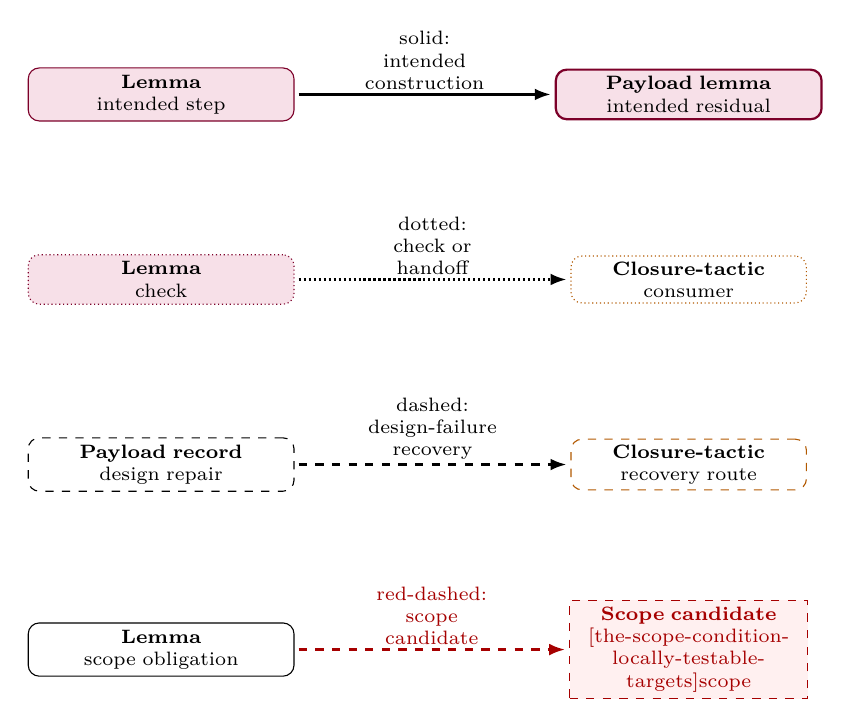
\begin{tikzpicture}[
every node/.style={font=\scriptsize},
leglabel/.style={bclabel,text width=2.25cm,align=center}
]
\node[bcbox,bclemma] (solidA) at (0,0) {\textbf{Lemma}\\intended step};
\node[bcbox,bclemma,bcpayload] (solidB) at (6.7,0) {\textbf{Payload lemma}\\intended residual};
\draw[bcarr] (solidA)--node[leglabel,above]{solid:\\intended\\construction}(solidB);
\node[bcbox,bclemma,bccheck] (checkA) at (0,-2.35) {\textbf{Lemma}\\check};
\node[bcroute,bcrouteneutral,bcoutputroute] (checkB) at (6.7,-2.35) {\textbf{Closure-tactic}\\consumer};
\draw[bchandoff] (checkA)--node[leglabel,above]{dotted:\\check or\\handoff}(checkB);
\node[bcbox,bcdesign] (repairA) at (0,-4.70) {\textbf{Payload record}\\design repair};
\node[bcroute,bcrouteneutral,bcdesign] (repairB) at (6.7,-4.70) {\textbf{Closure-tactic}\\recovery route};
\draw[bcrecoverarr] (repairA)--node[leglabel,above]{dashed:\\design-failure\\recovery}(repairB);
\node[bcbox] (scopeA) at (0,-7.05) {\textbf{Lemma}\\scope obligation};
\node[bcscopefail] (scopeB) at (6.7,-7.05) {\textbf{Scope candidate}\\\scoperef};
\draw[bcscopearr] (scopeA)--node[leglabel,above]{red-dashed:\\scope\\candidate}(scopeB);
\end{tikzpicture}
\caption[Line grammar legend]{Line grammar legend for the closure-tactic diagrams.}
\label{fig:line-grammar-legend}
\end{figure}

\subsection{Terminological conventions}\label{terminological-conventions}

The vocabulary of this document deliberately parallels standard
technique names, so that a first-time reader can anchor each concept to
something familiar:

\begin{itemize}
\tightlist
\item
  \textbf{charging schemes} generalize the charging and discharging
  arguments of extremal graph theory and computational geometry
  \citep{appel-haken-1977-discharging, appel-haken-koch-1977-reducibility, cranston-west-2017-discharging};
\item
  \textbf{local exchanges} generalize the exchange and switching
  arguments of extremal combinatorics;
\item
  \textbf{external types} are modeled on Myhill--Nerode-style context
  equivalence and on types in logic: two pieces have the same external type when no
  admissible surrounding context can tell them apart
  \citep{myhill-1957-automata, nerode-1958-linear, courcelle-1990-mso-graphs, courcelle-engelfriet-2012-graph-structure};
\item
  the \textbf{finite-state pumping principle} is a finite-state
  pigeonhole argument built from context equivalence
  \citep{myhill-1957-automata, nerode-1958-linear};
\item
  \textbf{compression} and \textbf{replacement} are used in the same
  spirit as protrusion replacement in kernelization
  \citep{bodlaender-etal-2009-meta-kernelization, kim-etal-2012-protrusion, garnero-etal-2013-explicit-kernels, jansen-wulms-2016-lower-bounds}.
\end{itemize}

Matching, star, pigeonhole, fibre, minor, and immersion retain their
standard meanings. Each method-specific term is defined in bold at first
occurrence and repeated in the glossary
(\appref{appendix-a.-glossary}).

Throughout, \(G\) denotes the ambient object under analysis (a graph,
colouring, hypergraph, matroid, etc., depending on the problem). A
\textbf{piece} is a subobject of \(G\) considered together with a
controlled interface; a tactic may impose an additional cardinality
bound. Formally, it is a \textbf{boundaried piece}
\((X,\partial X, \text{interface data})\), where \(\partial X\) is the
boundary along which \(X\) attaches to the rest of \(G\). An
\textbf{attachment point} is a designated vertex or element of that
boundary. A piece is \textbf{proper} if it is not all of \(G\). The
distinct notions of residual condition, residual class, and payload
instance are defined in \secref{data-branch-states} and
\secref{data-payloads}.

\textbf{Failure-classification convention.} The entry boundary separates
three audit outcomes. Execution errors \((E)\), such as an
unfilled equivalence or an unrecorded handoff, are audit rejects written to
the defect register. Repairable design failures \((D)\), such as a
missing finite label or an admissibility gap, are recovery-output
fields. A local nonexistence is a candidate scope issue for the current
tactic, not a terminal proof leaf. It becomes a scope obstruction \((S)\)
only after the global scope audit has established that no admitted tactic or
finite descriptor or proof-language extension can encode the residual. It is
terminal only after the defect register has ruled out a level-4 language
extension.

\paragraph{Certificate recap.}
The success leaves use the five certificate classes defined in
\secref{data-certificate-alphabet}.

\paragraph{Library closure claim.}
For every tactic CT\(k\), each non-certificate output is a named
payload accepted by the trigger of another CT entry, and the master
interlock graph contains the corresponding edge.  The only terminal
success classes are C1--C5. Candidate scope obstructions are not residual
outputs or immediate terminals; they are referred to the global audit in
\secref{the-scope-condition-locally-testable-targets}.

\paragraph{Invocation contract.}
Given an admitted CT invocation whose trigger and parameters are
recorded, execute its listed procedure, discharge its obligation
schemas, and return exactly one declared certificate or typed residual
payload on each resulting leaf.  Proposal, admission, selection,
repetition, and composition are governed by
\secref{part-iii-the-strategy-manual}.

\paragraph{Typed residual payloads.}
Each intended or recovery inter-tactic edge below is a typed handoff.  A
label \(P_{i\to j}\) means that CT\(i\) constructs the displayed tuple
and that the trigger of CT\(j\) accepts exactly that tuple.  Intended
payloads are the ordinary forward residuals in the tactic graph;
recovery payloads are dashed design-failure routes in the CT diagrams.
Concatenating two diagrams is therefore a type check: the producer must
discharge routing for the tuple, and the receiving tactic must discharge
trigger for the same tuple.  The CT entries use the following payloads.

\begingroup
\tiny
\setlength{\tabcolsep}{1pt}
\begin{longtable}[]{@{}
  >{\raggedright\arraybackslash}p{0.10\linewidth}
  >{\raggedright\arraybackslash}p{0.08\linewidth}
  >{\raggedright\arraybackslash}p{0.08\linewidth}
  >{\raggedright\arraybackslash}p{0.50\linewidth}
  >{\raggedright\arraybackslash}p{0.18\linewidth}@{}}
\toprule\noalign{}
Payload & Route class & To & Typed tuple & Description \\
\midrule\noalign{}
\endhead
\bottomrule\noalign{}
\endlastfoot
\(P_{1\to2}\) & Intended & CT2 & \(\langle\mathfrak B_{\neg T},X,\partial X,\iota_X,\preceq_0\rangle\) & Target-avoiding branch state, proper admissible piece, certified interface, and root order. \\
\(P_{1\to3}\) & Intended & CT3 & \(\langle\mathfrak B_{\neg T},X,\partial X,\iota_X,\tau\text{-slot},\text{exit flags}\rangle\) & Boundary-response datum ready for external typing. \\
\(P_{1\to4}\) & Intended & CT4 & \(\langle\mathfrak B_{\neg T},\mathcal D,\mathcal P,\pi,C,\ell\rangle\) & Demand set, payer set, canonical assignment rule, capacity bound, and lower-bound target. \\
\(P_{1\to5}\) & Intended & CT5 & \(\langle\mathfrak B_{\neg T},\mathcal S,\lambda_{\mathcal S},w,\mathcal L\rangle\) & Linear local-site family, site labels, witness extractor, and locality record. \\
\(P_{1\to6}\) & Intended & CT6 & \(\langle\mathfrak B_{\neg T},\mathcal A,\theta,\text{activity threshold},\text{first-failure extractor}\rangle\) & Active/dormant setup generated after target avoidance. \\
\(P_{1\to17}\) & Intended & CT17 & \(\langle\mathfrak B_{\neg T},S,\Delta,\Omega,\text{sparse target arithmetic}\rangle\) & Sparse target set, bounded offset family, and compatible completion data. \\
\(P_{2\to3}\) & Recovery & CT3 & \(\langle\mathfrak B,X,\partial X,\iota_X,\tau(X),\text{context residual}\rangle\) & Context-dependent response left by minimality. \\
\(P_{2\to10}\) & Recovery & CT10 & \(\langle\mathfrak B,X,\text{criticality datum},\text{missing finite label}\rangle\) & Target-uncompressible survivor requiring refinement. \\
\(P_{3\to7}\) & Intended & CT7 & \(\langle\mathfrak B,X,X',\iota,C_{\rm sep},\text{response pair}\rangle\) & Separating-context defect/exchange datum. \\
\(P_{3\to12}\) & Intended & CT12 & \(\langle\mathfrak B,L,\mu,\text{defect account}\rangle\) & Routed load with well-founded peel measure. \\
\(P_{3\to8}\) & Intended & CT8 & \(\langle\mathfrak B,(X_0,\ldots,X_m),\tau,\text{finite labels}\rangle\) & Long repeated-type sequence. \\
\(P_{4\to9}\) & Intended & CT9 & \(\langle\mathfrak B,\mathcal D,\mathcal P,\pi,C,p,\pi^{-1}(p),\text{labels}\rangle\) & Overcharged payer fibre. \\
\(P_{4\to14}\) & Intended & CT14 & \(\langle\mathfrak B,\mathcal R,\ell,\text{capacity record}\rangle\) & Aggregate residual class with carried mass. \\
\(P_{4\to13}\) & Recovery & CT13 & \(\langle\mathfrak B,\mathcal D_{\rm tier},A,O,\text{tier-interaction record}\rangle\) & Demand with no available payer, promoted to a tiered availability obstruction. \\
\(P_{5\to4}\) & Intended & CT4 & \(\langle\mathfrak B,\mathcal D_{\mathcal S},\mathcal P_{\mathcal S},\pi_{\mathcal S},C_{\mathcal S},\ell_{\mathcal S}\rangle\) & Charge map assembled from local witnesses. \\
\(P_{5\to11}\) & Intended & CT11 & \(\langle\mathfrak B,R,B(\cdot),\text{admissible decomposition}\rangle\) & Additive global-deficit residual. \\
\(P_{5\to14}\) & Intended & CT14 & \(\langle\mathfrak B,\mathcal R,\ell_{\mathcal R},\text{aggregate capacity record}\rangle\) & Local-mass shortfall residual. \\
\(P_{5\to C4}\) & Cert. & C4 & C4 certificate & Summed lower bound, capacity upper bound, and positive slack. \\
\(P_{6\to4}\) & Intended & CT4 & \(\langle\mathfrak B,\mathcal D_{\rm act},\mathcal P_{\rm act},\pi_{\rm act},C_{\rm act},\ell_{\rm act}\rangle\) & Active-test demand ledger. \\
\(P_{6\to7}\) & Intended & CT7 & \(\langle\mathfrak B,A,A',\iota,\delta,\text{first-failure witness}\rangle\) & Same-interface witness produced by dormancy. \\
\(P_{6\to3}\) & Intended & CT3 & \(\langle\mathfrak B,X,\partial X,\iota_X,\tau\text{-slot},\text{witness flags}\rangle\) & Boundary-response witness from the first failure. \\
\(P_{6\to9}\) & Intended & CT9 & \(\langle\mathfrak B,\mathcal D,\mathcal P,\pi,C,p,F_p,\text{saturation label}\rangle\) & Saturated payer or overload witness. \\
\(P_{6\to10}\) & Recovery & CT10 & \(\langle\mathfrak B,\text{first-failure witness},\text{missing refinement datum}\rangle\) & Bounded first-failure witness that appears only after refinement. \\
\(P_{7\to3}\) & Intended & CT3 & \(\langle\mathfrak B,A,A',\iota,C_{\rm sep},\text{response pair}\rangle\) & Distinguishing exchange as an external-type defect. \\
\(P_{7\to12}\) & Intended & CT12 & \(\langle\mathfrak B,L,\mu,\text{exchange-defect account}\rangle\) & Distinguishing exchange already packaged as peelable load. \\
\(P_{7\to10}\) & Recovery & CT10 & \(\langle\mathfrak B,A,A',\iota,\text{neutral label}\rangle\) & Neutral noncompressive exchange needing refinement. \\
\(P_{7\to16}\) & Recovery & CT16 & \(\langle\mathfrak B,Z=G,\tau_{\rm closed},\text{neutral closed data}\rangle\) & Neutral datum whose support is the whole object. \\
\(P_{8\to3}\) & Intended & CT3 & \(\langle\mathfrak B,S_i,S_j,C_{\rm sep},\tau_i,\tau_j\rangle\) & Separating context for repeated states. \\
\(P_{8\to7}\) & Intended & CT7 & \(\langle\mathfrak B,A,A',\iota,\delta,\text{chain exchange}\rangle\) & Exchange extracted from a long chain. \\
\(P_{8\to10}\) & Recovery & CT10 & \(\langle\mathfrak B,(S_0,\ldots,S_m),\allowbreak\text{coarse finite labels},\allowbreak\text{missing refinement datum}\rangle\) & Finite label space requiring a certified refinement before pumping. \\
\(P_{9\to4}\) & Intended & CT4 & \(\langle\mathfrak B,\mathcal D,\mathcal P,\pi,C,\text{bounded-fibre proof}\rangle\) & Bounded multiplicity returned to charging. \\
\(P_{9\to7}\) & Intended & CT7 & \(\langle\mathfrak B,A,A',\iota,\delta,\text{homogeneous fibre witness}\rangle\) & Same-interface object extracted from overload. \\
\(P_{9\to8}\) & Intended & CT8 & \(\langle\mathfrak B,(S_0,\ldots,S_m),\tau,\text{homogeneous chain labels}\rangle\) & Long chain extracted from overload. \\
\(P_{9\to10}\) & Recovery & CT10 & \(\langle\mathfrak B,F_p,\text{failed finite label design},\text{refinement datum}\rangle\) & Label refinement needed for the overloaded fibre. \\
\(P_{10\to7}\) & Intended & CT7 & \(\langle\mathfrak B,\mathcal C_\ell,A,A',\iota,\text{class exchange}\rangle\) & Bounded exchange inside a refined label class. \\
\(P_{10\to3}\) & Intended & CT3 & \(\langle\mathfrak B,\mathcal C_\ell,X,\partial X,\iota_X,\tau\text{-slot}\rangle\) & Promoted response/type datum. \\
\(P_{10\to15}\) & Intended & CT15 & \(\langle\mathfrak B,\mathcal C_\ell,r,\text{rank datum}\rangle\) & Promoted rank datum for forcing. \\
\(P_{11\to10}\) & Recovery & CT10 & \(\langle\mathfrak B,X,\text{admissibility gap},\text{finite local type slot}\rangle\) & Localized piece outside the admissible toolbox. \\
\(P_{11\to1}\) & Intended & CT1 & \(\langle\mathfrak B,X,T,\mathcal T,\text{localized target witness}\rangle\) & Localized deficit piece carrying target-test data. \\
\(P_{11\to7}\) & Intended & CT7 & \(\langle\mathfrak B,A,A',\iota,\delta,\text{localized exchange}\rangle\) & Localized piece carrying a bounded exchange. \\
\(P_{11\to14}\) & Intended & CT14 & \(\langle\mathfrak B,\mathcal R,\ell_{\mathcal R},\text{localized carried mass}\rangle\) & Localized deficit converted to aggregate mass. \\
\(P_{12\to4}\) & Recovery & CT4 & \(\langle\mathfrak B,\mathcal D_{\rm new},\mathcal P_{\rm new},\pi_{\rm new},C_{\rm new},\ell_{\rm new}\rangle\) & Restored state with an ordinary new demand. \\
\(P_{12\to13}\) & Recovery & CT13 & \(\langle\mathfrak B,\mathcal D_{\rm tier},A,O,\text{tier-interaction record}\rangle\) & Restored state whose new demand requires tiered charging. \\
\(P_{13\to4}\) & Intended & CT4 & \(\langle\mathfrak B,\mathcal D,\mathcal P_1,\pi_1,C_1,\ell_1\rangle\) & Tier-one charge account. \\
\(P_{13\to9}\) & Intended & CT9 & \(\langle\mathfrak B,p,F_p,\text{overlap obstruction labels}\rangle\) & Overlap obstruction as a fibre overload. \\
\(P_{13\to14}\) & Intended & CT14 & \(\langle\mathfrak B,\mathcal R,\ell_{\mathcal R},\text{overlap mass record}\rangle\) & Overlap obstruction as aggregate mass. \\
\(P_{14\to9}\) & Recovery & CT9 & \(\langle\mathfrak B,u,\text{unbounded capacity member},\text{multiplicity gap}\rangle\) & Aggregate multiplicity failure routed to overload. \\
\(P_{14\to10}\) & Recovery & CT10 & \(\langle\mathfrak B,\mathcal C,\text{finite missing capacity datum},\text{refinement slot}\rangle\) & Aggregate capacity record requiring a finite pointwise refinement. \\
\(P_{15\to3}\) & Intended & CT3 & \(\langle\mathfrak B,X,\partial X,\iota_X,\tau\text{-slot},\text{rank defect}\rangle\) & Rank-drop dependence as type defect. \\
\(P_{15\to7}\) & Intended & CT7 & \(\langle\mathfrak B,A,A',\iota,\delta,\text{rank exchange}\rangle\) & Rank-drop dependence as exchange or compression data. \\
\(P_{15\to16}\) & Intended & CT16 & \(\langle\mathfrak B,Z=G,\tau_{\rm closed},\text{rank delocalization}\rangle\) & Rank-drop dependence that is whole-object. \\
\(P_{15\to4}\) & Intended & CT4 & \(\langle\mathfrak B,\mathcal D_{\rm rank},\mathcal P_{\rm rank},\pi_{\rm rank},C_{\rm rank},\ell_{\rm rank}\rangle\) & Full-rank demand ledger. \\
\(P_{16\to3}\) & Intended & CT3 & \(\langle\mathfrak B,X,\partial X,\iota_X,\tau(X),\substack{\text{proper subpiece}\\\text{from the whole-object split}}\rangle\) & Proper subpiece from the whole-object dichotomy. \\
\(P_{16\to10}\) & Intended & CT10 & \(\langle\mathfrak B,Z=G,\tau_{\rm closed}^{(1)},\tau_{\rm closed}^{(2)},\text{distinct data}\rangle\) & Distinct closed-type residual. \\
\(P_{17\to3}\) & Recovery & CT3 & \(\langle\mathfrak B,\mathcal K,\iota,\tau\text{-slot},\text{incompatible completion class}\rangle\) & Completion class separated by type. \\
\(P_{17\to10}\) & Recovery & CT10 & \(\langle\mathfrak B,\mathcal K,\ell,\text{incompatible completion class}\rangle\) & Completion class separated by label. \\
\(P_{17\to8}\) & Intended & CT8 & \(\langle\mathfrak B,(S_0,\ldots,S_m),\tau,\text{finite survivor offsets}\rangle\) & Finite survivor list for pumping/exhaustion. \\
\(P_{17\to14}\) & Intended & CT14 & \(\langle\mathfrak B,\mathcal R,\ell_{\mathcal R},\text{arithmetic residual mass}\rangle\) & Target-thickening residual mass. \\
\end{longtable}
\endgroup

\subsection{The master interlock graph}\label{the-master-interlock-graph}
The following figures are part of the tactic library in \secref{part-ii-the-tactic-library}.  The first
is the expanded interlock map; the second suppresses closure sinks and
scope boundaries to show only inter-tactic residual routing.

\begin{figure}[p]
\centering
\resizebox{\textwidth}{!}{%
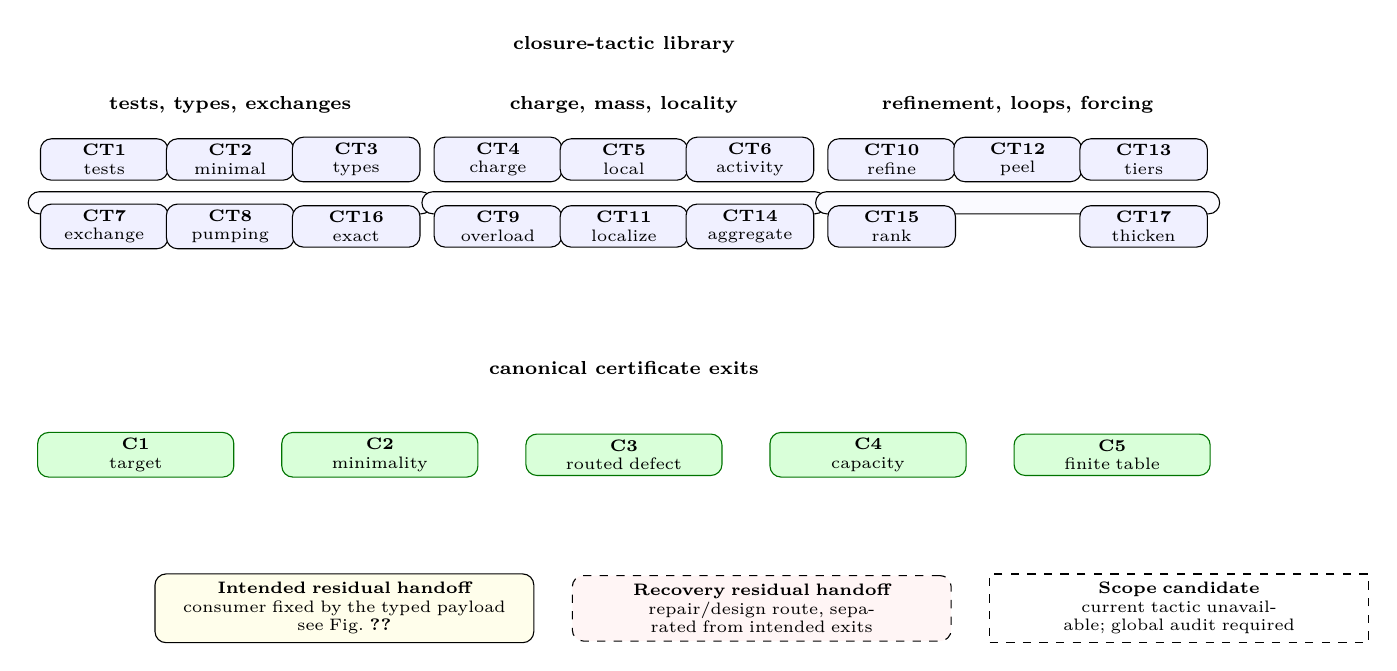
\begin{tikzpicture}[
x=1cm,
y=1cm,
every node/.style={font=\fontsize{6.0}{6.7}\selectfont},
groupbox/.style={rectangle,rounded corners,draw,fill=blue!2,align=center,inner sep=4pt,minimum width=4.85cm,text width=4.85cm},
chip/.style={rectangle,rounded corners,draw,fill=blue!6,align=center,inner sep=2pt,minimum width=1.48cm,text width=1.48cm},
sink/.style={rectangle,rounded corners,draw=green!45!black,fill=green!15,align=center,inner sep=2pt,minimum width=2.35cm,text width=2.35cm},
routebox/.style={rectangle,rounded corners,draw,fill=yellow!8,align=center,inner sep=3pt,minimum width=4.60cm,text width=4.60cm},
recoverbox/.style={rectangle,rounded corners,draw,dashed,fill=red!4,align=center,inner sep=3pt,minimum width=4.60cm,text width=4.60cm},
scopebox/.style={rectangle,draw,dashed,align=center,inner sep=3pt,minimum width=4.60cm,text width=4.60cm},
head/.style={font=\fontsize{6.8}{7.4}\selectfont\bfseries,align=center},
arr/.style={-{Latex[length=1.6mm]},thin,shorten <=2pt,shorten >=2pt},
darr/.style={-{Latex[length=1.6mm]},thin,dashed,shorten <=2pt,shorten >=2pt}
]
\node[head] at (0,0.85) {closure-tactic library};
\node[groupbox] (testgroup) at (-5.0,-1.15) {};
\node[groupbox] (chargegroup) at (0,-1.15) {};
\node[groupbox] (refinegroup) at (5.0,-1.15) {};

\node[head] at (-5.0,0.10) {tests, types, exchanges};
\node[chip] at (-6.60,-0.60) {\textbf{CT1}\\tests};
\node[chip] at (-5.00,-0.60) {\textbf{CT2}\\minimal};
\node[chip] at (-3.40,-0.60) {\textbf{CT3}\\types};
\node[chip] at (-6.60,-1.45) {\textbf{CT7}\\exchange};
\node[chip] at (-5.00,-1.45) {\textbf{CT8}\\pumping};
\node[chip] at (-3.40,-1.45) {\textbf{CT16}\\exact};

\node[head] at (0,0.10) {charge, mass, locality};
\node[chip] at (-1.60,-0.60) {\textbf{CT4}\\charge};
\node[chip] at (0,-0.60) {\textbf{CT5}\\local};
\node[chip] at (1.60,-0.60) {\textbf{CT6}\\activity};
\node[chip] at (-1.60,-1.45) {\textbf{CT9}\\overload};
\node[chip] at (0,-1.45) {\textbf{CT11}\\localize};
\node[chip] at (1.60,-1.45) {\textbf{CT14}\\aggregate};

\node[head] at (5.0,0.10) {refinement, loops, forcing};
\node[chip] at (3.40,-0.60) {\textbf{CT10}\\refine};
\node[chip] at (5.00,-0.60) {\textbf{CT12}\\peel};
\node[chip] at (6.60,-0.60) {\textbf{CT13}\\tiers};
\node[chip] at (3.40,-1.45) {\textbf{CT15}\\rank};
\node[chip] at (6.60,-1.45) {\textbf{CT17}\\thicken};

\node[head] at (0,-3.25) {canonical certificate exits};
\node[sink] (c1) at (-6.20,-4.35) {\textbf{C1}\\target};
\node[sink] (c2) at (-3.10,-4.35) {\textbf{C2}\\minimality};
\node[sink] (c3) at (0,-4.35) {\textbf{C3}\\routed defect};
\node[sink] (c4) at (3.10,-4.35) {\textbf{C4}\\capacity};
\node[sink] (c5) at (6.20,-4.35) {\textbf{C5}\\finite table};

\node[routebox] (intended) at (-3.55,-6.30) {\textbf{Intended residual handoff}\\consumer fixed by the typed payload\\see Fig.~\ref{fig:closure-tactic-routing-graph}};
\node[recoverbox] (recovery) at (1.75,-6.30) {\textbf{Recovery residual handoff}\\repair/design route, separated from intended exits};
\node[scopebox] (scope) at (7.05,-6.30) {\textbf{Scope candidate}\\current tactic unavailable; global audit required};
\end{tikzpicture}%
}
\caption[Closure-tactic interlock diagram]{Closure-tactic interlock diagram.  The blue chips are the seventeen closure tactics grouped by their role in the library.  Every admitted CT execution exits through one of the displayed interfaces: a canonical certificate C1--C5, an intended residual handoff, a recovery residual handoff, or a candidate obstruction referred to the global scope audit in \secref{the-scope-condition-locally-testable-targets}.  The split inventory and Fig.~\ref{fig:closure-tactic-routing-graph} give the payload names and consumers; following a residual handoff requires routing at the producer and trigger at the named consumer.}
\label{fig:closure-tactic-interlock}
\end{figure}

\clearpage

\begin{figure}[p]
\centering
\resizebox{\textwidth}{!}{%
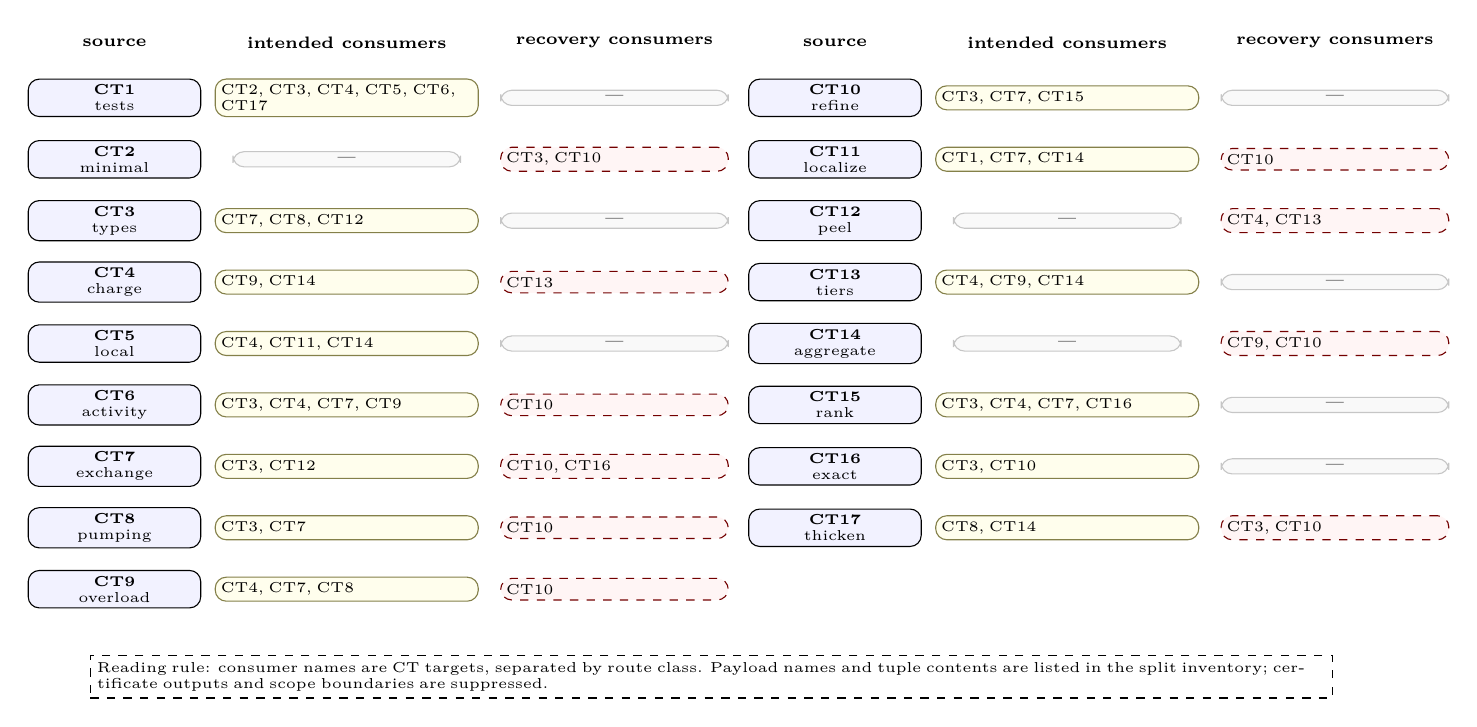
\begin{tikzpicture}[
x=1cm,
y=1cm,
every node/.style={font=\fontsize{5.2}{5.8}\selectfont},
rsource/.style={rectangle,rounded corners,draw,fill=blue!5,align=center,inner sep=2.0pt,minimum width=2.05cm,text width=2.05cm},
rint/.style={rectangle,rounded corners,draw=yellow!45!black,fill=yellow!7,align=left,inner sep=2.0pt,minimum width=3.20cm,text width=3.20cm},
rrec/.style={rectangle,rounded corners,draw=red!45!black,dashed,fill=red!4,align=left,inner sep=2.0pt,minimum width=2.75cm,text width=2.75cm},
rnone/.style={rectangle,rounded corners,draw=gray!45,fill=gray!5,align=center,inner sep=2.0pt,minimum width=2.75cm,text width=2.75cm},
rghead/.style={font=\fontsize{6.0}{6.6}\selectfont\bfseries,align=center},
rglegend/.style={rectangle,draw,dashed,align=left,inner sep=2.5pt,minimum width=15.6cm,text width=15.6cm}
]
\node[rghead] at (0,0.70) {source};
\node[rghead] at (2.95,0.70) {intended consumers};
\node[rghead] at (6.35,0.70) {recovery consumers};
\node[rghead] at (9.15,0.70) {source};
\node[rghead] at (12.10,0.70) {intended consumers};
\node[rghead] at (15.50,0.70) {recovery consumers};

\node[rsource] at (0,0) {\textbf{CT1}\\tests};
\node[rint] at (2.95,0) {CT2, CT3, CT4, CT5, CT6, CT17};
\node[rnone] at (6.35,0) {---};
\node[rsource] at (0,-0.78) {\textbf{CT2}\\minimal};
\node[rnone] at (2.95,-0.78) {---};
\node[rrec] at (6.35,-0.78) {CT3, CT10};
\node[rsource] at (0,-1.56) {\textbf{CT3}\\types};
\node[rint] at (2.95,-1.56) {CT7, CT8, CT12};
\node[rnone] at (6.35,-1.56) {---};
\node[rsource] at (0,-2.34) {\textbf{CT4}\\charge};
\node[rint] at (2.95,-2.34) {CT9, CT14};
\node[rrec] at (6.35,-2.34) {CT13};
\node[rsource] at (0,-3.12) {\textbf{CT5}\\local};
\node[rint] at (2.95,-3.12) {CT4, CT11, CT14};
\node[rnone] at (6.35,-3.12) {---};
\node[rsource] at (0,-3.90) {\textbf{CT6}\\activity};
\node[rint] at (2.95,-3.90) {CT3, CT4, CT7, CT9};
\node[rrec] at (6.35,-3.90) {CT10};
\node[rsource] at (0,-4.68) {\textbf{CT7}\\exchange};
\node[rint] at (2.95,-4.68) {CT3, CT12};
\node[rrec] at (6.35,-4.68) {CT10, CT16};
\node[rsource] at (0,-5.46) {\textbf{CT8}\\pumping};
\node[rint] at (2.95,-5.46) {CT3, CT7};
\node[rrec] at (6.35,-5.46) {CT10};
\node[rsource] at (0,-6.24) {\textbf{CT9}\\overload};
\node[rint] at (2.95,-6.24) {CT4, CT7, CT8};
\node[rrec] at (6.35,-6.24) {CT10};

\node[rsource] at (9.15,0) {\textbf{CT10}\\refine};
\node[rint] at (12.10,0) {CT3, CT7, CT15};
\node[rnone] at (15.50,0) {---};
\node[rsource] at (9.15,-0.78) {\textbf{CT11}\\localize};
\node[rint] at (12.10,-0.78) {CT1, CT7, CT14};
\node[rrec] at (15.50,-0.78) {CT10};
\node[rsource] at (9.15,-1.56) {\textbf{CT12}\\peel};
\node[rnone] at (12.10,-1.56) {---};
\node[rrec] at (15.50,-1.56) {CT4, CT13};
\node[rsource] at (9.15,-2.34) {\textbf{CT13}\\tiers};
\node[rint] at (12.10,-2.34) {CT4, CT9, CT14};
\node[rnone] at (15.50,-2.34) {---};
\node[rsource] at (9.15,-3.12) {\textbf{CT14}\\aggregate};
\node[rnone] at (12.10,-3.12) {---};
\node[rrec] at (15.50,-3.12) {CT9, CT10};
\node[rsource] at (9.15,-3.90) {\textbf{CT15}\\rank};
\node[rint] at (12.10,-3.90) {CT3, CT4, CT7, CT16};
\node[rnone] at (15.50,-3.90) {---};
\node[rsource] at (9.15,-4.68) {\textbf{CT16}\\exact};
\node[rint] at (12.10,-4.68) {CT3, CT10};
\node[rnone] at (15.50,-4.68) {---};
\node[rsource] at (9.15,-5.46) {\textbf{CT17}\\thicken};
\node[rint] at (12.10,-5.46) {CT8, CT14};
\node[rrec] at (15.50,-5.46) {CT3, CT10};

\node[rglegend] at (7.58,-7.35) {Reading rule: consumer names are CT targets, separated by route class.  Payload names and tuple contents are listed in the split inventory; certificate outputs and scope boundaries are suppressed.};
\end{tikzpicture}%
}
\caption[Closure-tactic routing graph]{Closure-tactic routing graph.  Each row lists one source tactic, its intended residual consumers, and its recovery-route consumers in separate columns.  The typed payload names and tuple contents are listed in the split inventory before Fig.~\ref{fig:closure-tactic-interlock}; following any row entry requires routing at the source and trigger at the named target.  Closure outputs and candidate obstructions referred to the global scope audit in \secref{the-scope-condition-locally-testable-targets} are suppressed here so that only inter-tactic dependencies remain.}
\label{fig:closure-tactic-routing-graph}
\end{figure}

\noindent\textbf{CT1-start typed-payload flow.}
The next figure records the tactics reachable from CT1 by declared
typed payloads.  Each CT appears once.  An arrow \(P_{i\to j}\) means
that CT\(i\) has constructed the exact payload accepted by CT\(j\).
Each directed path carries its own cumulative branch-state extension;
outgoing edges are alternative continuations, and a cycle returns with
newly recorded data or progress. CT6 and CT17 are reachable from
CT1 through the activity-setup payload \(P_{1\to6}\) and the sparse-target
offset payload \(P_{1\to17}\).

\begin{figure}[p]
\centering
\vspace*{-1.60cm}
\resizebox{\textwidth}{!}{%
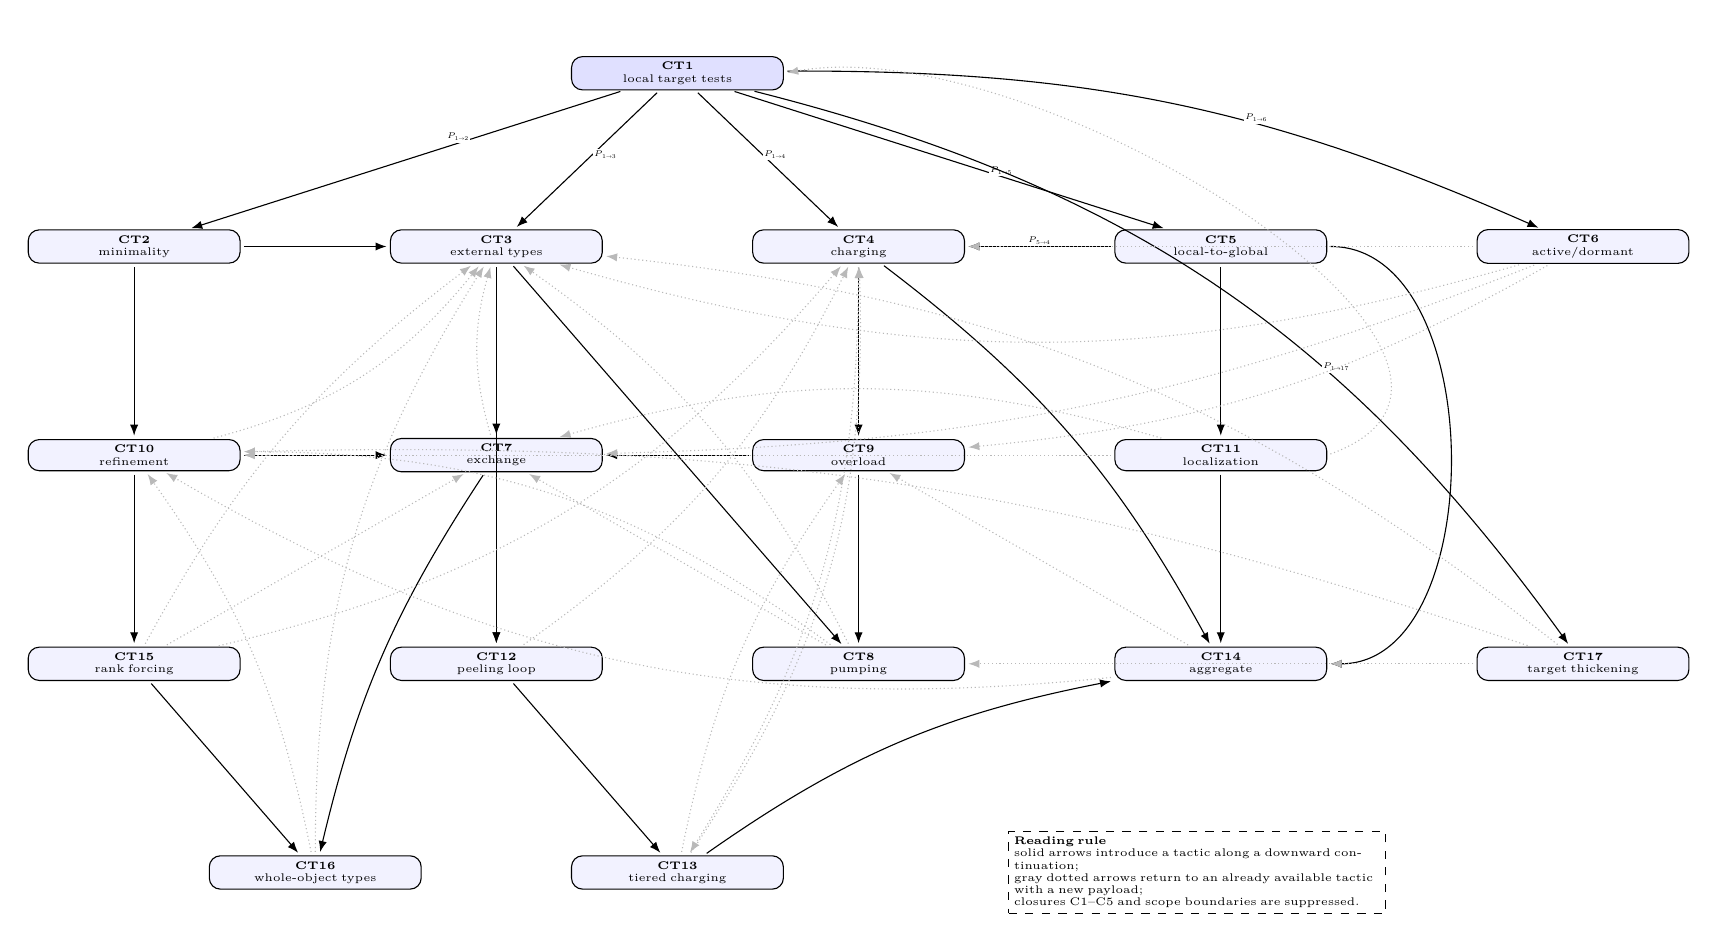
\begin{tikzpicture}[
x=1cm,
y=1cm,
every node/.style={font=\fontsize{4.0}{4.4}\selectfont},
flowstart/.style={rectangle,rounded corners,draw,fill=blue!12,align=center,inner sep=2pt,minimum width=2.55cm,text width=2.55cm},
flowtactic/.style={rectangle,rounded corners,draw,fill=blue!5,align=center,inner sep=2pt,minimum width=2.55cm,text width=2.55cm},
flowlegend/.style={rectangle,draw,dashed,align=left,inner sep=2pt,minimum width=4.65cm,text width=4.65cm},
flowarr/.style={-{Latex[length=1.4mm]},thin,shorten <=1.2pt,shorten >=1.2pt},
flowback/.style={-{Latex[length=1.4mm]},thin,densely dotted,draw=gray!55,shorten <=1.2pt,shorten >=1.2pt},
flowlbl/.style={font=\fontsize{3.0}{3.3}\selectfont,inner sep=0.6pt,fill=white}
]
\node[flowstart] (ct1) at (0,0) {\textbf{CT1}\\local target tests};
\node[flowtactic] (ct2) at (-6.90,-2.20) {\textbf{CT2}\\minimality};
\node[flowtactic] (ct3) at (-2.30,-2.20) {\textbf{CT3}\\external types};
\node[flowtactic] (ct4) at (2.30,-2.20) {\textbf{CT4}\\charging};
\node[flowtactic] (ct5) at (6.90,-2.20) {\textbf{CT5}\\local-to-global};
\node[flowtactic] (ct6) at (11.50,-2.20) {\textbf{CT6}\\active/dormant};

\node[flowtactic] (ct10) at (-6.90,-4.85) {\textbf{CT10}\\refinement};
\node[flowtactic] (ct7) at (-2.30,-4.85) {\textbf{CT7}\\exchange};
\node[flowtactic] (ct9) at (2.30,-4.85) {\textbf{CT9}\\overload};
\node[flowtactic] (ct11) at (6.90,-4.85) {\textbf{CT11}\\localization};

\node[flowtactic] (ct15) at (-6.90,-7.50) {\textbf{CT15}\\rank forcing};
\node[flowtactic] (ct12) at (-2.30,-7.50) {\textbf{CT12}\\peeling loop};
\node[flowtactic] (ct8) at (2.30,-7.50) {\textbf{CT8}\\pumping};
\node[flowtactic] (ct14) at (6.90,-7.50) {\textbf{CT14}\\aggregate};
\node[flowtactic] (ct17) at (11.50,-7.50) {\textbf{CT17}\\target thickening};

\node[flowtactic] (ct16) at (-4.60,-10.15) {\textbf{CT16}\\whole-object types};
\node[flowtactic] (ct13) at (0,-10.15) {\textbf{CT13}\\tiered charging};
\node[flowlegend] (legend) at (6.60,-10.15) {\textbf{Reading rule}\\
solid arrows introduce a tactic along a downward continuation;\\
gray dotted arrows return to an already available tactic with a new payload;\\
closures C1--C5 and scope boundaries are suppressed.};

\draw[flowarr] (ct1) -- node[flowlbl,above,pos=.38]{\(P_{1\to2}\)} (ct2);
\draw[flowarr] (ct1) -- node[flowlbl,right,pos=.46]{\(P_{1\to3}\)} (ct3);
\draw[flowarr] (ct1) -- node[flowlbl,right,pos=.46]{\(P_{1\to4}\)} (ct4);
\draw[flowarr] (ct1) -- node[flowlbl,above,pos=.62]{\(P_{1\to5}\)} (ct5);
\draw[flowarr] (ct1) to[bend left=12] node[flowlbl,above,pos=.62]{\(P_{1\to6}\)} (ct6);
\draw[flowarr] (ct1) to[bend left=20] node[flowlbl,right,pos=.64]{\(P_{1\to17}\)} (ct17);

\draw[flowarr] (ct2) -- (ct10);
\draw[flowarr] (ct2) -- (ct3);

\draw[flowarr] (ct3) -- (ct7);
\draw[flowarr] (ct3) -- (ct12);
\draw[flowarr] (ct3) -- (ct8);

\draw[flowarr] (ct4) -- (ct9);
\draw[flowarr] (ct4) to[bend left=12] (ct14);
\draw[flowback] (ct4) to[bend left=16] (ct13);

\draw[flowarr] (ct5) -- node[flowlbl,above]{\(P_{5\to4}\)} (ct4);
\draw[flowarr] (ct5) -- (ct11);
\draw[flowarr] (ct5.east) to[out=0,in=0] (ct14.east);

\draw[flowarr] (ct10) -- (ct15);
\draw[flowarr] (ct10) -- (ct7);
\draw[flowback] (ct10) to[bend right=18] (ct3);

\draw[flowback] (ct7) to[bend left=16] (ct3);
\draw[flowarr] (ct7) -- (ct12);
\draw[flowback] (ct7) -- (ct10);
\draw[flowarr] (ct7) to[bend right=10] (ct16);

\draw[flowback] (ct9) -- (ct4);
\draw[flowarr] (ct9) -- (ct7);
\draw[flowarr] (ct9) -- (ct8);

\draw[flowback] (ct11.west) to[out=180,in=0] (ct10.east);
\draw[flowback] (ct11) to[bend right=16] (ct7);
\draw[flowarr] (ct11) -- (ct14);
\draw[flowback] (ct11.east) to[out=20,in=10] (ct1.east);

\draw[flowback] (ct15) to[bend left=12] (ct3);
\draw[flowback] (ct15) to[bend right=18] (ct4);
\draw[flowback] (ct15) -- (ct7);
\draw[flowarr] (ct15) -- (ct16);

\draw[flowarr] (ct12) -- (ct13);
\draw[flowback] (ct12) to[bend right=14] (ct4);

\draw[flowback] (ct8) to[bend right=14] (ct3);
\draw[flowback] (ct8) -- (ct7);
\draw[flowback] (ct8) to[bend right=18] (ct10);

\draw[flowback] (ct14) -- (ct9);
\draw[flowback] (ct14) to[bend left=18] (ct10);

\draw[flowback] (ct6) to[bend left=16] (ct3);
\draw[flowback] (ct6) -- (ct4);
\draw[flowback] (ct6) to[bend left=10] (ct7);
\draw[flowback] (ct6) to[bend left=12] (ct9);

\draw[flowback] (ct17) to[bend right=16] (ct3);
\draw[flowback] (ct17) to[bend right=10] (ct10);
\draw[flowback] (ct17) -- (ct8);
\draw[flowback] (ct17) -- (ct14);

\draw[flowback] (ct16) to[bend left=16] (ct3);
\draw[flowback] (ct16) to[bend right=12] (ct10);

\draw[flowback] (ct13) to[bend right=18] (ct4);
\draw[flowback] (ct13) to[bend left=12] (ct9);
\draw[flowarr] (ct13) to[bend left=12] (ct14);
\end{tikzpicture}%
}
\caption[CT1-start typed-payload flow]{CT1-start typed-payload flow.  The figure shows the CT tactics reachable from CT1 by declared payloads in the tactic-library table of \secref{part-ii-the-tactic-library}, with each CT represented by a single node.  Direct CT1\(\to\)CT4 is present because \(P_{1\to4}\) is already a complete charging payload; CT5\(\to\)CT4 is the distinct route in which local witnesses assemble the charging payload \(P_{5\to4}\).  CT6 is reachable through \(P_{1\to6}\), the activity-setup payload, and CT17 is reachable through \(P_{1\to17}\), the sparse-target offset payload.  Gray dotted arrows are re-entry edges to tactics already present in the cumulative flow; their payload names are listed in the typed-payload table.}
\label{fig:ct1-continuation-flow}
\end{figure}

\clearpage


\paragraph{Sequential inventory.}
The table below is the controlling description of the tactic
library.  The home column points to the detailed entry and its diagram;
the CT entries are indexed here in numerical order, and each caption is
part of the corresponding tactic specification.

\begingroup
\tiny
\setlength{\tabcolsep}{1.1pt}
\begin{longtable}[]{@{}
  >{\raggedright\arraybackslash}p{0.06\linewidth}
  >{\raggedright\arraybackslash}p{0.18\linewidth}
  >{\raggedright\arraybackslash}p{0.24\linewidth}
  >{\raggedright\arraybackslash}p{0.10\linewidth}
  >{\raggedright\arraybackslash}p{0.24\linewidth}
  >{\raggedright\arraybackslash}p{0.14\linewidth}@{}}
\toprule\noalign{}
ID & Tactic & Home and diagram & Certificates & Intended residuals & Recovery residuals \\
\midrule\noalign{}
\endhead
\bottomrule\noalign{}
\endlastfoot
CT1 & Local target tests & \secref{target-predicate-and-local-tests}, Fig.~\ref{fig:ct1-local-target-tests} & C1 & \(P_{1\to2}\), \(P_{1\to3}\), \(P_{1\to4}\), \(P_{1\to5}\), \(P_{1\to6}\), \(P_{1\to17}\) & --- \\
CT2 & Minimality and replacement & \secref{minimal-counterexample}, Fig.~\ref{fig:ct2-minimality-replacement} & C2 & --- & \(P_{2\to3}\), \(P_{2\to10}\) \\
CT3 & External-type compression & \secref{boundaried-pieces-and-external-types}, Fig.~\ref{fig:ct3-external-type-compression} & C2, C3, C5 & \(P_{3\to7}\), \(P_{3\to12}\), \(P_{3\to8}\) & --- \\
CT4 & Charging schemes & \secref{charging-schemes}, Fig.~\ref{fig:ct4-charging-schemes} & C4 & \(P_{4\to9}\), \(P_{4\to14}\) & \(P_{4\to13}\) \\
CT5 & Local-to-global bookkeeping & \secref{the-local-versus-global-rationale}, Fig.~\ref{fig:ct5-local-global-bookkeeping} & C4 & \(P_{5\to4}\), \(P_{5\to11}\), \(P_{5\to14}\) & --- \\
CT6 & Active/dormant dichotomy & \secref{the-activedormant-dichotomy}, Fig.~\ref{fig:ct6-active-dormant} & C1 & \(P_{6\to4}\), \(P_{6\to3}\), \(P_{6\to7}\), \(P_{6\to9}\) & \(P_{6\to10}\) \\
CT7 & Exchange trichotomy & \secref{the-exchange-trichotomy}, Fig.~\ref{fig:ct7-exchange-trichotomy} & C1, C2, C3 & \(P_{7\to3}\), \(P_{7\to12}\) & \(P_{7\to10}\), \(P_{7\to16}\) \\
CT8 & Finite-state pumping & \secref{the-finite-state-pumping-principle}, Fig.~\ref{fig:ct8-finite-state-pumping} & C2, C5 & \(P_{8\to3}\), \(P_{8\to7}\) & \(P_{8\to10}\) \\
CT9 & Overload exhaustion & \secref{the-charging-principle-in-general-form}, Fig.~\ref{fig:ct9-overload-exhaustion} & C1 & \(P_{9\to4}\), \(P_{9\to7}\), \(P_{9\to8}\) & \(P_{9\to10}\) \\
CT10 & Default refinement & \secref{the-default-refinement}, Fig.~\ref{fig:ct10-default-refinement} & C5 & \(P_{10\to3}\), \(P_{10\to7}\), \(P_{10\to15}\) & --- \\
CT11 & Localization & \secref{additivity-and-the-localization-lemma}, Fig.~\ref{fig:ct11-localization} & --- & \(P_{11\to1}\), \(P_{11\to7}\), \(P_{11\to14}\) & \(P_{11\to10}\) \\
CT12 & Peeling loop & \secref{peeling-loops-closure-by-well-founded-recursion}, Fig.~\ref{fig:ct12-peeling-loop} & C4 & --- & \(P_{12\to4}\), \(P_{12\to13}\) \\
CT13 & Tiered charging & \secref{tiered-charging-scheme-failure-as-a-demand}, Fig.~\ref{fig:ct13-tiered-charging} & C4 & \(P_{13\to4}\), \(P_{13\to9}\), \(P_{13\to14}\) & --- \\
CT14 & Aggregate closure & \secref{aggregate-closure-mass-bounds-on-residual-classes}, Fig.~\ref{fig:ct14-aggregate-closure} & C4 & --- & \(P_{14\to9}\), \(P_{14\to10}\) \\
CT15 & Rank forcing & \secref{rank-forcing-charge-only-independent-coordinates}, Fig.~\ref{fig:ct15-rank-forcing} & C4 & \(P_{15\to3}\), \(P_{15\to4}\), \(P_{15\to7}\), \(P_{15\to16}\) & --- \\
CT16 & Whole-object exact types & \secref{the-whole-object-piece-exact-types-under-context-degeneracy}, Fig.~\ref{fig:ct16-whole-object-types} & C2 & \(P_{16\to3}\), \(P_{16\to10}\) & --- \\
CT17 & Target thickening & \secref{target-thickening-bounded-offsets-against-sparse-targets}, Fig.~\ref{fig:ct17-target-thickening} & C1, C5 & \(P_{17\to8}\), \(P_{17\to14}\) & \(P_{17\to3}\), \(P_{17\to10}\) \\
\end{longtable}
\endgroup

\paragraph{Mechanism-entry ledger.}
The next table is the per-entry audit ledger. It does not replace the
figures; it makes the fields needed for format compliance explicit in a
single lookup location. The procedure field is deliberately schematic:
the numbered mathematical objects and arrows are the corresponding
diagram.

\begingroup
\scriptsize
\setlength{\tabcolsep}{1.2pt}
\begin{longtable}[]{@{}
  >{\raggedright\arraybackslash}p{0.06\linewidth}
  >{\raggedright\arraybackslash}p{0.17\linewidth}
  >{\raggedright\arraybackslash}p{0.18\linewidth}
  >{\raggedright\arraybackslash}p{0.20\linewidth}
  >{\raggedright\arraybackslash}p{0.16\linewidth}
  >{\raggedright\arraybackslash}p{0.16\linewidth}@{}}
\toprule\noalign{}
ID & Purpose & Trigger & Parameters & Audit hooks & Candidate scope obstruction \\
\midrule\noalign{}
\endhead
\bottomrule\noalign{}
\endlastfoot
CT1 & Convert target realization into C1 or target-avoiding payloads. & Local test family, witness spaces, and target equivalence recorded. & Test family, witness extractor, branch-state record. & Reject missing equivalence; write target-avoidance row and payload row. & No local test family exists. \\
CT2 & Apply minimality by deletion, replacement, or target-uncompressible routing. & Proper admissible piece in a minimal counterexample. & Size order, admissibility class, replacement family. & Reject undeclared interface; write deletion-critical and uncompressible rows. & No bounded interface exists. \\
CT3 & Compare external types and route defects, tables, or peelable load. & Certified interface and type slot recorded. & Context universe, type evaluator, replacement table. & Reject unproved equivalence; write type-table or defect-account row. & No finite type index exists. \\
CT4 & Turn a demand/payer ledger into C4 or a typed capacity residual. & Demand set, payer set, assignment rule, capacity, and lower bound recorded. & Canonical assignment rule, capacity proof, lower-bound estimate. & Reject non-deterministic assignment; write ledger, capacity, or missing-tier rows. & No locally generated demand exists. \\
CT5 & Sum local witnesses into a global charge, budget, or localized residual. & Linear local-site family with witness extractor recorded. & Site labels, local lower bound, summation domain. & Reject missing locality lemma; write summation and slack rows. & No bounded local witness exists. \\
CT6 & Split active tests from first-failure dormant structure. & Activity threshold and first-failure extractor recorded. & Activity predicate, threshold, first-failure order. & Reject unrecorded threshold data; write active ledger or witness row. & No bounded first-failure witness exists. \\
CT7 & Classify a bounded exchange as realizing, distinguishing, or neutral. & Unclassified exchange pair on a certified common interface. & Context generator, response evaluator, size order, table handle. & Reject neutral claim with equivalence unfilled; write exchange classification row. & No finite context generator exists. \\
CT8 & Pump a bounded sequence through finite labels or exact types. & Bounded sequence with finite label/type slot recorded. & Label alphabet, equality test, finite threshold. & Reject informal periodicity; write repeat, table, or label-refinement row. & No finite type space exists. \\
CT9 & Exhaust an overloaded payer fibre by homogeneous extraction. & Payer fibre and capacity bound recorded. & Label map, fibre capacity, extraction target. & Reject unlabelled fibre; write overload and extraction row. & No finite labelling exists. \\
CT10 & Promote a missing finite datum to a refinement label. & Residual class exposing a finite missing datum. & Candidate datum, refined label alphabet, class table. & Reject datum not extracted from classification; write refinement row. & No finite refinement alphabet exists. \\
CT11 & Localize an additive global deficit to an admissible piece. & Additive budget deficit and admissible decomposition recorded. & Budget, admissibility class, decomposition lemma. & Reject nonadditive budget; write localization or admissibility-gap row. & No additive bounded local type exists. \\
CT12 & Peel routed load by a well-founded loop. & Routed load account and measure recorded. & Peel move, restoration map, measure. & Reject failed S-Rest or S-Meas; write per-pass and termination rows. & No measurable load exists. \\
CT13 & Split a failed charge into tiered accounts or overlap residuals. & Tier-one account or obstruction record present. & Tier split, availability test, reconciliation rule. & Reject unrecorded tier overlap; write tier ledger and overlap row. & No measurable tier resource exists. \\
CT14 & Close a residual class by linear mass versus sublinear capacity. & Residual class with lower mass and candidate capacity record. & Class mass lower bound, member capacity, aggregate upper bound. & Reject unbounded multiplicity; write aggregate, overload, or finite-refinement row. & No bounded capacity description exists. \\
CT15 & Charge only target-independent rank coordinates. & Target-relative rank datum recorded. & Rank map, dependence classifier, full-rank ledger. & Reject incidental rank; write rank-drop or full-rank row. & No finite target-relative rank exists. \\
CT16 & Resolve whole-object cases by exact closed types. & Delocalized whole-object datum and computable closed type recorded. & Closed-type evaluator, equality test, proper-piece test. & Reject empty-context equivalence; write exact-type row. & No finitely computable closed type exists. \\
CT17 & Thicken sparse targets by bounded offsets and arithmetic residuals. & Sparse target set and bounded offset family recorded. & Offset set, compatibility classes, survivor list. & Reject incompatible offsets without class record; write offset and survivor rows. & No bounded offset family exists. \\
\end{longtable}
\endgroup

\paragraph{Signature and guarantee ledger.}
The complete entry for CT\(k\) is the union of the mechanism-entry row,
the signature-and-guarantee row below, and the diagram. Scheduler data are
a separate policy view consumed by \secref{part-iii-the-strategy-manual}.
This table records the template fields whose contents are easiest to
audit as formal arrows: Input, Obligations, Certificate, intended
outputs, and recovery outputs.
The Procedure field is the corresponding diagram read from top to
bottom.  Every intended non-terminal arrow listed here must appear in
that diagram and in the master interlock graph; every recovery arrow
must appear as a dashed design-failure route in the corresponding
diagram.

\begingroup
\tiny
\setlength{\tabcolsep}{0.8pt}
\begin{longtable}[]{@{}
  >{\raggedright\arraybackslash}p{0.055\linewidth}
  >{\raggedright\arraybackslash}p{0.23\linewidth}
  >{\raggedright\arraybackslash}p{0.22\linewidth}
  >{\raggedright\arraybackslash}p{0.10\linewidth}
  >{\raggedright\arraybackslash}p{0.18\linewidth}
  >{\raggedright\arraybackslash}p{0.15\linewidth}@{}}
\toprule\noalign{}
ID & Input & Obligations & Certificate & Intended outputs & Recovery outputs \\
\midrule\noalign{}
\endhead
\bottomrule\noalign{}
\endlastfoot
CT1 & \(\langle\mathfrak B,T,\mathcal T,W\rangle\) & definition\(\langle\mathcal T,W\rangle\); equivalence\(\langle T,\mathcal T\rangle\); S-Pers\(\langle T\)-avoidance\(\rangle\); routing; trigger. & C1, realized local test. & Target-avoiding payloads to CT2, CT3, CT4, CT5, CT6, CT17. & --- \\
CT2 & \(P_{1\to2}\) & definition\(\langle X,\iota_X,\prec\rangle\); dichotomy (delete, replace, survive); composition\(\langle\prec\rangle\); routing; trigger. & C2, minimality contradiction. & --- & Context residual to CT3; target-uncompressible datum to CT10. \\
CT3 & \(P_{\ast\to3}\) & definition\(\langle\iota,\tau\rangle\); equivalence\(\langle\tau\)-responses\(\rangle\); S-Pers; routing; trigger; composition. & C2, C3, or C5. & Exchange defect to CT7; peelable load to CT12; long type sequence to CT8. & --- \\
CT4 & \(P_{\ast\to4}\) & definition\(\langle\mathcal D,\mathcal P,\pi\rangle\); S-Det\(\langle\pi\rangle\); dichotomy (gap, overload); composition; routing; trigger. & C4, bounded-capacity contradiction. & Overcharged fibre to CT9; aggregate mass residual to CT14. & Missing payer tier to CT13. \\
CT5 & \(P_{1\to5}\) & definition\(\langle\mathcal S,w\rangle\); S-Det\(\langle\)site assignment\(\rangle\); composition\(\langle\)summation\(\rangle\); routing; trigger. & C4, local-to-global comparison. & Charge ledger to CT4; global deficit to CT11; aggregate residual to CT14. & --- \\
CT6 & \(P_{1\to6}\) & definition\(\langle\)activity threshold\(\rangle\); dichotomy (active, dormant); routing; trigger; equivalence\(\langle\)first failure\(\rangle\). & C1, first-failure target hit. & Active ledger to CT4; boundary/type witness to CT3; exchange witness to CT7; saturation witness to CT9. & Refinement-gated witness to CT10. \\
CT7 & \(P_{\ast\to7}\) & definition\(\langle\)exchange pair\(\rangle\); equivalence\(\langle\)context generator\(\rangle\); dichotomy (realizing, distinguishing, neutral); composition; routing; trigger. & C1, C2, or C3. & External-type defect to CT3; peelable defect to CT12. & Neutral label to CT10; whole-object datum to CT16. \\
CT8 & \(P_{\ast\to8}\) & definition (bounded sequence, type); dichotomy (repeat, short); equivalence\(\langle\)type equality\(\rangle\); composition; routing; trigger. & C2 or C5. & Separating type to CT3; chain exchange to CT7. & Coarse finite label space to CT10. \\
CT9 & \(P_{\ast\to9}\) & definition\(\langle F_p\rangle\); dichotomy (bounded, overloaded); composition\(\langle\)pigeonhole\(\rangle\); routing; trigger. & C1, target-hit overload. & Bounded multiplicity to CT4; homogeneous exchange to CT7; long chain to CT8. & Label-refinement residual to CT10. \\
CT10 & \(P_{\ast\to10}\) & definition\(\langle\)refined label\(\rangle\); dichotomy\(\langle\)label classes\(\rangle\); composition\(\langle\)finite table\(\rangle\); routing; trigger. & C5, finite class exhaustion. & Promoted response to CT3; class exchange to CT7; rank datum to CT15. & --- \\
CT11 & \(P_{5\to11}\) & definition (budget, decomposition); composition\(\langle\)localization\(\rangle\); routing; trigger. & None; route-only tactic. & Local target witness to CT1; localized exchange to CT7; carried mass to CT14. & Admissibility gap to CT10. \\
CT12 & \(P_{\ast\to12}\) & definition\(\langle L,\mu\rangle\); S-Rest; S-Meas; composition\(\langle\)termination\(\rangle\); routing; trigger. & C4, loop discharge. & --- & Restored ordinary demand to CT4; tiered demand to CT13. \\
CT13 & \(P_{\ast\to13}\) & definition\(\langle\)tiers\(\rangle\); S-Det\(\langle\)tier assignment\(\rangle\); dichotomy (availability, obstruction); composition; routing; trigger. & C4, reconciled tier capacity. & Tier-one account to CT4; overlap fibre to CT9; overlap mass to CT14. & --- \\
CT14 & \(P_{\ast\to14}\) & definition\(\langle\mathcal C\rangle\); composition\(\langle\)lower mass\(\rangle\); composition\(\langle\)upper capacity\(\rangle\); routing; trigger. & C4, aggregate capacity contradiction. & --- & Unbounded member or multiplicity gap to CT9; finite missing capacity datum to CT10. \\
CT15 & \(P_{\ast\to15}\) & definition\(\langle\)rank\(\rangle\); dichotomy (rank drop, full rank); composition\(\langle\)rank budget\(\rangle\); routing; trigger. & C4, rank-budget contradiction. & Rank defect to CT3; rank exchange to CT7; whole-object rank datum to CT16; rank ledger to CT4. & --- \\
CT16 & \(P_{\ast\to16}\) & definition\(\langle\)closed type\(\rangle\); equivalence\(\langle\)closed response\(\rangle\); dichotomy (proper, whole); composition; routing; trigger. & C2, exact whole-object identification. & Proper subpiece to CT3; distinct closed data to CT10. & --- \\
CT17 & \(P_{1\to17}\) & definition\(\langle S,\Delta,\Omega\rangle\); dichotomy\(\langle\)scale split\(\rangle\); composition\(\langle\)arithmetic\(\rangle\); routing; trigger. & C1 or C5. & Finite survivors to CT8; arithmetic mass to CT14. & Completion class to CT3 or CT10. \\
\end{longtable}
\endgroup

\paragraph{Scheduler data.}
The following data are published by the reference manual but are not
rules of execution. \secref{part-iii-the-strategy-manual} consumes these fields when it decides which
tactic to admit or select. The cost classes are: \texttt{check} for
steps whose parameters are already recorded and require no parameter
synthesis, \texttt{synth} for tactics
requiring manufactured parameters, and \texttt{loop} for tactics carrying
a well-founded measure. Producer fields name CTs except for CT1's unique
root input.

\begingroup
\tiny
\setlength{\tabcolsep}{0.7pt}
\begin{longtable}[]{@{}
  >{\raggedright\arraybackslash}p{0.055\linewidth}
  >{\raggedright\arraybackslash}p{0.055\linewidth}
  >{\raggedright\arraybackslash}p{0.17\linewidth}
  >{\raggedright\arraybackslash}p{0.14\linewidth}
  >{\raggedright\arraybackslash}p{0.17\linewidth}
  >{\raggedright\arraybackslash}p{0.14\linewidth}
  >{\raggedright\arraybackslash}p{0.22\linewidth}@{}}
\toprule\noalign{}
ID & Cost & Intended producers & Recovery producers & Intended consumers & Recovery consumers & Formal counterpart / [EG] anchor \\
\midrule\noalign{}
\endhead
\bottomrule\noalign{}
\endlastfoot
CT1 & check & root input, CT11 & --- & CT2, CT3, CT4, CT5, CT6, CT17 & --- & decidable local witness search; [EG] target tests \\
CT2 & check & CT1 & --- & --- & CT3, CT10 & minimality replacement lemma; [EG] criticality \\
CT3 & synth & CT1, CT6, CT7, CT8, CT10, CT15, CT16 & CT2, CT17 & CT7, CT8, CT12 & --- & finite type comparison; [EG] response profiles \\
CT4 & synth & CT1, CT5, CT6, CT9, CT13, CT15 & CT12 & CT9, CT14 & CT13 & charge-map capacity proof; [EG] ledgers \\
CT5 & synth & CT1 & --- & CT4, CT11, CT14 & --- & local summation proof; [EG] window and stub accounts \\
CT6 & synth & CT1 & --- & CT3, CT4, CT7, CT9 & CT10 & active/dormant classifier; [EG] hot/cold interface \\
CT7 & synth & CT3, CT6, CT8, CT9, CT10, CT11, CT15 & --- & CT3, CT12 & CT10, CT16 & decidable exchange classifier; [EG] germ routing \\
CT8 & synth & CT3, CT9, CT17 & --- & CT3, CT7 & CT10 & finite-state/pumping table; [EG] trace basin \\
CT9 & check & CT4, CT6, CT13 & CT14 & CT4, CT7, CT8 & CT10 & pigeonhole over finite fibres; [EG] overload extraction \\
CT10 & synth & CT16 & CT2, CT6, CT7, CT8, CT9, CT11, CT14, CT17 & CT3, CT7, CT15 & --- & finite label refinement; [EG] label classes \\
CT11 & synth & CT5 & --- & CT1, CT7, CT14 & CT10 & additive localization lemma; [EG] net-charge localization \\
CT12 & loop & CT3, CT7 & --- & --- & CT4, CT13 & well-founded recursion; [EG] routed-load peeling \\
CT13 & synth & --- & CT4, CT12 & CT4, CT9, CT14 & --- & tiered discharging proof; [EG] type-B ledgers \\
CT14 & synth & CT4, CT5, CT11, CT13, CT17 & --- & --- & CT9, CT10 & aggregate capacity comparison; [EG] bridge residuals \\
CT15 & synth & CT10 & --- & CT3, CT4, CT7, CT16 & --- & rank independence proof; [EG] curvature rank \\
CT16 & synth & CT15 & CT7 & CT3, CT10 & --- & exact closed-type computation; [EG] whole-graph profiles \\
CT17 & synth & CT1 & --- & CT8, CT14 & CT3, CT10 & bounded-offset arithmetic; [EG] sparse target thickening \\
\end{longtable}
\endgroup

\paragraph{Schema coverage by tactic.}
The detailed diagrams instantiate these schemas as named mathematical
objects.  This table records the obligation vocabulary that must be
discharged when each tactic is used.

\begingroup
\scriptsize
\setlength{\tabcolsep}{2pt}
\begin{longtable}[]{@{}
  >{\raggedright\arraybackslash}p{0.08\linewidth}
  >{\raggedright\arraybackslash}p{0.84\linewidth}@{}}
\toprule\noalign{}
ID & Primary schemas \\
\midrule\noalign{}
\endhead
\bottomrule\noalign{}
\endlastfoot
CT1 & definition, equivalence, dichotomy, S-Pers, routing, trigger. \\
CT2 & definition, dichotomy, composition, routing, trigger. \\
CT3 & definition, equivalence, S-Pers, routing, trigger. \\
CT4 & definition, S-Det, dichotomy, composition, routing, trigger. \\
CT5 & definition, S-Det, composition, routing, trigger. \\
CT6 & definition, dichotomy, routing, trigger. \\
CT7 & definition, equivalence, dichotomy, composition, routing, trigger. \\
CT8 & definition, dichotomy, equivalence, composition, routing, trigger. \\
CT9 & definition, dichotomy, composition, routing, trigger. \\
CT10 & definition, dichotomy, routing, trigger. \\
CT11 & definition, composition, routing, trigger. \\
CT12 & definition, dichotomy, S-Pers, S-Rest, S-Meas, routing, trigger. \\
CT13 & definition, S-Det, dichotomy, composition, routing, trigger. \\
CT14 & definition, composition, routing, trigger. \\
CT15 & definition, dichotomy, composition, routing, trigger. \\
CT16 & definition, equivalence, dichotomy, routing, trigger. \\
CT17 & definition, dichotomy, composition, routing, trigger. \\
\end{longtable}
\endgroup
\subsection{CT1 --- Local target tests}\label{ct:1}\label{target-predicate-and-local-tests}
\ctsignature{\(\langle\mathfrak B,T,\mathcal T,W\rangle \to
\ctcert{C1};\allowbreak\ \ctint{P_{1\to2},\allowbreak P_{1\to3},\allowbreak P_{1\to4},\allowbreak P_{1\to5},\allowbreak P_{1\to6},\allowbreak P_{1\to17}};\allowbreak\ \ctrec{\ctnone}\).}

CT1 consumes a branch state carrying target-test data, either from the
proof instance or from the typed localization payload emitted by CT11.
The tactic turns the theorem's target predicate into a finite family of
local tests and publishes the target-avoiding state when none of them is
realized.

\ctpar{Fires when}
The branch state records a target predicate \(T\), a local test family
\(\mathcal T\), and witness spaces \(W_i(G)\).  Entry is syntactic: the
objects are present in the state and await the equivalence check.

\ctpar{You supply}
The supplied parameters are the local test family, the witness extractor,
and the branch-state record in which all tests are absent.  The radius of
the tests is synthesized by the scope and local-test rules of \secref{part-iii-the-strategy-manual}:
it must be large enough to witness \(T\) and small enough to have finite
interface type.

\ctpar{Execution}
Prove test equivalence as two separate lemmas.  The easy direction says
that a realized test gives the target.  The load-bearing direction says
that every target realization contains one of the chosen witnesses.  Once
equivalence is certified, split on whether some \(T_i\) is realized.  A
realized test closes immediately; absence of all tests defines the
target-avoiding state \(\mathfrak B_{\neg T}\).  Each certified datum
surviving that absence is packaged by the corresponding payload
constructor listed under Routing.  Part III orders simultaneously
available payloads.

\ctpar{Soundness obligations}
\begin{itemize}
\tightlist
\item \textbf{definition} is instantiated with the target predicate \(T\), the local test family \(\mathcal T\), the witness spaces \(W_i(G)\), and the witness extractor recorded in the branch state.
\item \textbf{equivalence} is instantiated with the equivalence between \(T\) and the existence of a realized local test \(T_i\).
\item \textbf{S-Pers} is instantiated with the transition from the current state to \(\mathfrak B_{\neg T}\), where all local tests are absent.
\item \textbf{routing} is instantiated with the target-avoiding payloads \(P_{1\to2}\), \(P_{1\to3}\), \(P_{1\to4}\), \(P_{1\to5}\), \(P_{1\to6}\), and \(P_{1\to17}\).
\item \textbf{trigger} is instantiated with the consumer trigger for each target-avoiding payload emitted by CT1.
\end{itemize}

\ctpar{Routing}
The C1 exit is the realized local test.  Otherwise CT1 emits typed
target-avoiding payloads: a proper reducible piece to CT2, a
boundary-response datum to CT3, a completed charge ledger to CT4, a
linear local-site family to CT5, an activity setup to CT6, or sparse
offset data to CT17.  The selection among simultaneously certified
payloads follows \secref{selection-policy}.

\ctpar{Limit}
CT1 is inapplicable when no local test family is available. This is a
candidate obstruction for the global audit in
\secref{the-scope-condition-locally-testable-targets}, not a residual branch. The execution error
is claiming target avoidance without equivalence; the audit records it as a
CT1/equivalence defect.

\begin{figure}[p]
\centering
\vspace*{-2.80cm}
\resizebox{!}{0.68\textheight}{%
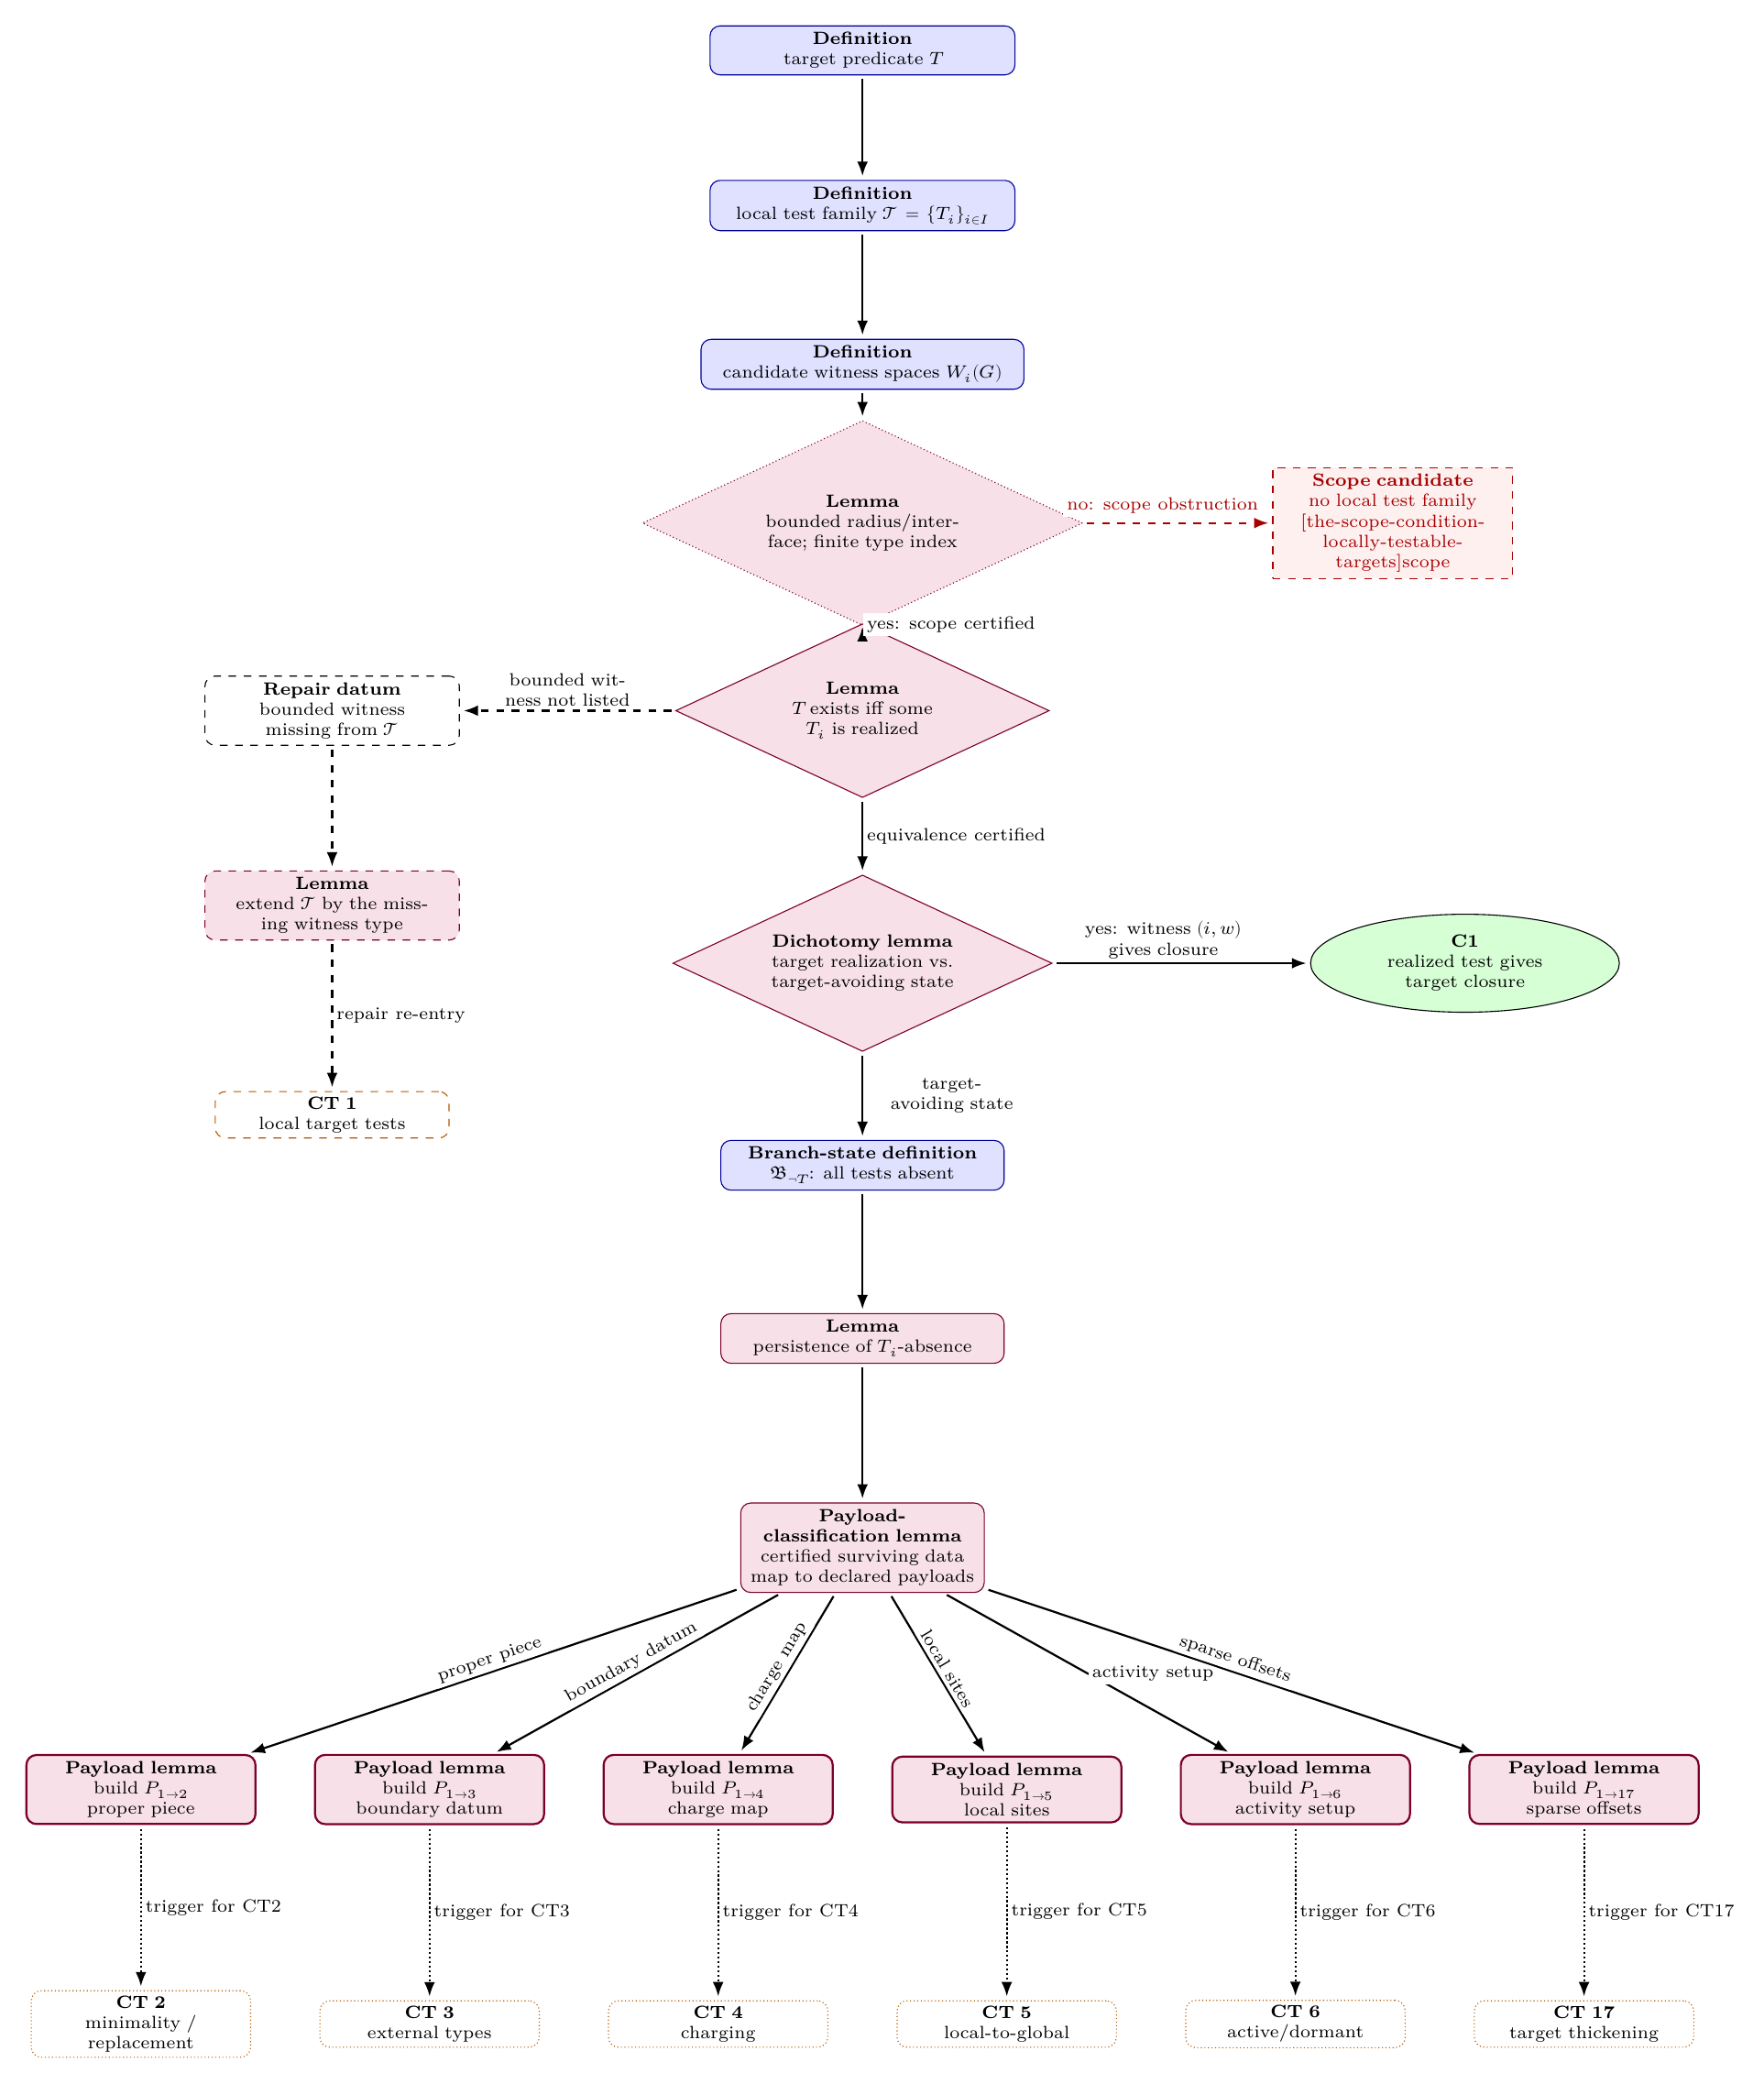
\begin{tikzpicture}[
x=1cm,
y=1cm,
every node/.style={font=\scriptsize}
]
\node[bcwide,bcdefinition] (target) at (0,0.60) {\textbf{Definition}\\target predicate \(T\)};
\node[bcwide,bcdefinition] (tests) at (0,-1.55) {\textbf{Definition}\\local test family \(\mathcal T=\{T_i\}_{i\in I}\)};
\node[bcwide,bcdefinition,text width=4.30cm,minimum width=4.30cm] (witness) at (0,-3.75) {\textbf{Definition}\\candidate witness spaces \(W_i(G)\)};
\node[bcauditbox,text width=4.20cm,minimum width=4.20cm] (scope) at (0,-5.95) {\textbf{Lemma}\\bounded radius/interface; finite type index};
\node[bcscopefail,text width=3.15cm,minimum width=3.15cm] (scopebad) at (7.35,-5.95) {\textbf{Scope candidate}\\no local test family\\\scoperef};
\node[bcdec,bclemma,text width=3.25cm,minimum width=3.95cm] (complete) at (0,-8.55) {\textbf{Lemma}\\\(T\) exists iff some \(T_i\) is realized};
\node[bcbox,bcdesign,text width=3.35cm,minimum width=3.35cm] (testgap) at (-7.35,-8.55) {\textbf{Repair datum}\\bounded witness missing from \(\mathcal T\)};
\node[bcbox,bclemma,bcdesign,text width=3.35cm,minimum width=3.35cm] (testlemma) at (-7.35,-11.25) {\textbf{Lemma}\\extend \(\mathcal T\) by the missing witness type};
\node[bcroute,bcrouteneutral,bcdesign,text width=3.10cm,minimum width=3.10cm] (testroute) at (-7.35,-14.15) {\textbf{CT 1}\\local target tests};
\node[bcdec,bclemma,text width=3.35cm,minimum width=4.15cm] (hitq) at (0,-12.05) {\textbf{Dichotomy lemma}\\target realization vs.\ target-avoiding state};
\node[bcclosed] (hit) at (8.35,-12.05) {\textbf{C1}\\realized test gives target closure};
\node[bcbox,bcdefinition,text width=3.75cm,minimum width=3.75cm] (avoid) at (0,-14.85) {\textbf{Branch-state definition}\\\(\mathfrak B_{\neg T}\): all tests absent};
\node[bcbox,bclemma,text width=3.75cm,minimum width=3.75cm] (register) at (0,-17.25) {\textbf{Lemma}\\persistence of \(T_i\)-absence};
\node[bcbox,bclemma] (next) at (0,-20.15) {\textbf{Payload-classification lemma}\\certified surviving data map to declared payloads};
\node[bcbox,bclemma,bcpayload,text width=3.00cm,minimum width=3.00cm] (minlemma) at (-10.00,-23.50) {\textbf{Payload lemma}\\build \(P_{1\to2}\)\\proper piece};
\node[bcbox,bclemma,bcpayload,text width=3.00cm,minimum width=3.00cm] (typelemma) at (-6.00,-23.50) {\textbf{Payload lemma}\\build \(P_{1\to3}\)\\boundary datum};
\node[bcbox,bclemma,bcpayload,text width=3.00cm,minimum width=3.00cm] (chargelemma) at (-2.00,-23.50) {\textbf{Payload lemma}\\build \(P_{1\to4}\)\\charge map};
\node[bcbox,bclemma,bcpayload,text width=3.00cm,minimum width=3.00cm] (sitelemma) at (2.00,-23.50) {\textbf{Payload lemma}\\build \(P_{1\to5}\)\\local sites};
\node[bcbox,bclemma,bcpayload,text width=3.00cm,minimum width=3.00cm] (activelemma) at (6.00,-23.50) {\textbf{Payload lemma}\\build \(P_{1\to6}\)\\activity setup};
\node[bcbox,bclemma,bcpayload,text width=3.00cm,minimum width=3.00cm] (thicklemma) at (10.00,-23.50) {\textbf{Payload lemma}\\build \(P_{1\to17}\)\\sparse offsets};
\node[bcroute,bcrouteneutral,bcoutputroute,text width=2.90cm,minimum width=2.90cm] (minroute) at (-10.00,-26.75) {\textbf{CT 2}\\minimality / replacement};
\node[bcroute,bcrouteneutral,bcoutputroute,text width=2.90cm,minimum width=2.90cm] (typeroute) at (-6.00,-26.75) {\textbf{CT 3}\\external types};
\node[bcroute,bcrouteneutral,bcoutputroute,text width=2.90cm,minimum width=2.90cm] (chargeroute) at (-2.00,-26.75) {\textbf{CT 4}\\charging};
\node[bcroute,bcrouteneutral,bcoutputroute,text width=2.90cm,minimum width=2.90cm] (siteroute) at (2.00,-26.75) {\textbf{CT 5}\\local-to-global};
\node[bcroute,bcrouteneutral,bcoutputroute,text width=2.90cm,minimum width=2.90cm] (activeroute) at (6.00,-26.75) {\textbf{CT 6}\\active/dormant};
\node[bcroute,bcrouteneutral,bcoutputroute,text width=2.90cm,minimum width=2.90cm] (thickroute) at (10.00,-26.75) {\textbf{CT 17}\\target thickening};
\draw[bcarr] (target)--(tests);
\draw[bcarr] (tests)--(witness);
\draw[bcarr] (witness)--(scope);
\draw[bcscopearr] (scope)--node[bclabel,above,sloped,pos=.42,yshift=2pt]{no: scope obstruction}(scopebad);
\draw[bcarr] (scope)--node[bclabel,right]{yes: scope certified}(complete);
\draw[bcrecoverarr] (complete)--node[bclabel,above,text width=2.35cm,align=center]{bounded witness not listed}(testgap);
\draw[bcrecoverarr] (testgap)--(testlemma);
\draw[bcrecoverarr] (testlemma)--node[bclabel,right]{repair re-entry}(testroute);
\draw[bcarr] (complete)--node[bclabel,right]{equivalence certified}(hitq);
\draw[bcarr] (hitq)--node[bclabel,above,pos=0.43,text width=2.70cm,align=center]{yes: witness \((i,w)\) gives closure}(hit);
\draw[bcarr] (hitq)--node[bclabel,right,text width=2.35cm,align=center]{target-avoiding state}(avoid);
\draw[bcarr] (avoid)--(register);
\draw[bcarr] (register)--(next);
\draw[bcarr] (next)--node[bclabel,above,sloped]{proper piece}(minlemma);
\draw[bcarr] (next)--node[bclabel,above,sloped]{boundary datum}(typelemma);
\draw[bcarr] (next)--node[bclabel,above,sloped]{charge map}(chargelemma);
\draw[bcarr] (next)--node[bclabel,above,sloped]{local sites}(sitelemma);
\draw[bcarr] (next)--node[bclabel,right]{activity setup}(activelemma);
\draw[bcarr] (next)--node[bclabel,above,sloped]{sparse offsets}(thicklemma);
\draw[bchandoff] (minlemma)--node[bclabel,right]{trigger for CT2}(minroute);
\draw[bchandoff] (typelemma)--node[bclabel,right]{trigger for CT3}(typeroute);
\draw[bchandoff] (chargelemma)--node[bclabel,right]{trigger for CT4}(chargeroute);
\draw[bchandoff] (sitelemma)--node[bclabel,right]{trigger for CT5}(siteroute);
\draw[bchandoff] (activelemma)--node[bclabel,right]{trigger for CT6}(activeroute);
\draw[bchandoff] (thicklemma)--node[bclabel,right]{trigger for CT17}(thickroute);
\end{tikzpicture}%
}
\caption[Closure-tactic 1: local target tests]{Closure-tactic 1 (local target tests).  The diagram is an object-level proof checklist: the target enters through definitions of \(T\), \(\mathcal T\), and the witness spaces \(W_i(G)\), a scope lemma, an equivalence lemma, a target-realization dichotomy lemma, a realization proposition, a definition of the target-avoiding branch state, a persistence lemma for \(T_i\)-absence, a payload-classification lemma mapping each certified surviving datum to its declared payload, and payload lemmas certifying the inputs to the next closure-tactic diagrams.  The six non-closing exits are typed: \(P_{1\to2}\) routes a proper reducible piece to CT2, \(P_{1\to3}\) routes boundary-response data to CT3, \(P_{1\to4}\) routes a ready demand/payer charge map to CT4, \(P_{1\to5}\) routes a linear local-site family to CT5, \(P_{1\to6}\) routes an activity-threshold setup to CT6, and \(P_{1\to17}\) routes sparse-target offset data to CT17.  Absence of a local test family is a candidate scope obstruction referred to the global audit in \secref{the-scope-condition-locally-testable-targets}.  Line grammar (Fig.~\ref{fig:line-grammar-legend}): solid --- intended execution through the construction of the intended residual; dotted --- checks and the post-residual handoff to the consumer tactic; dashed --- design-failure recovery; red-dashed --- candidate scope obstruction referred to the global audit.}
\label{fig:ct1-local-target-tests}
\end{figure}
\FloatBarrier

\subsection*{Local target tests in practice}

Start with a \textbf{target predicate} \(T\): the property whose
existence the theorem asserts. Depending on the problem, the target may
be the existence of a prescribed substructure, a monochromatic
configuration, a flow, colouring, matching, or minor, or a
moment-accessible spectral consequence such as a walk-count or girth
condition. A spectral-gap target requires a cut or energy residual
interface rather than only bounded-radius forbidden-pattern tests; see
\secref{the-scope-condition-locally-testable-targets}.

CT1 represents the target predicate by a family of
\textbf{local tests}

\[
\mathcal T = \{T_i\}_{i\in I}
\qquad\text{such that}\qquad
\text{target exists} \iff \exists\, i \in I \text{ with } T_i \text{ realized},
\]

where a test is \textbf{realized} if some configuration in \(G\)
satisfies it. The tests must be local enough to interact with small
pieces, yet complete enough that target avoidance is expressible as a
conjunction of local exclusions.

The low-level diagram for CT1 is Fig.~\ref{fig:ct1-local-target-tests};
it turns this paragraph into the required definitions, lemmas, closure
leaf, and typed residual exits.



\subsection{CT2 --- Minimality and replacement}\label{ct:2}\label{minimal-counterexample}
\ctsignature{\(P_{1\to2}\to \ctcert{C2};\ \ctint{\ctnone};\ \ctrec{P_{2\to3},P_{2\to10}}\).}

You typically reach CT2 from CT1 after target avoidance exposes a proper
piece that may be deleted or replaced.  The tactic is the disciplined use
of minimality: it closes legal reductions and routes the survivor when
minimality leaves a target-uncompressible object.

\ctpar{Fires when}
The state contains a minimal counterexample, a proper admissible piece
with interface data, and a declared size order.  The trigger is the
presence of a deletion or replacement candidate in that recorded state.

\ctpar{You supply}
You supply the size order, the admissibility class, and the replacement
family.  These come from the resource inventory and from the interface
vocabulary data; the replacement family must be compatible with the
recorded outside contexts.

\ctpar{Execution}
Run two branches.  The deletion branch proves that removing the piece
preserves the baseline hypotheses and decreases the size order.  The
replacement branch first proves context universality for the proposed
substitute and only then compares sizes.  If either branch is legal,
minimality gives C2.  If both fail in a typed way, the failed context or
the uncompressible survivor becomes the next payload.

\ctpar{Soundness obligations}
\begin{itemize}
\tightlist
\item \textbf{definition} is instantiated with the proper piece \(X\), its interface \(\iota_X\), the admissibility class, and the minimality order \(\prec\).
\item \textbf{dichotomy} is instantiated with the three alternatives that \(X\) can be deleted, replaced, or kept as a surviving residual.
\item \textbf{composition} is instantiated with the proof that every legal deletion or replacement produces an object strictly smaller in the order \(\prec\).
\item \textbf{routing} is instantiated with \(P_{2\to3}\) for a context-dependent response and \(P_{2\to10}\) for a target-uncompressible survivor.
\item \textbf{trigger} is instantiated with the CT3 trigger for context residuals and the CT10 trigger for target-uncompressible data.
\end{itemize}

\ctpar{Routing}
Legal deletion or replacement closes by C2.  A context-dependent
response emits \(P_{2\to3}\) to CT3.  A target-uncompressible survivor
with a missing finite label emits \(P_{2\to10}\) to CT10.

\ctpar{Limit}
CT2 is inapplicable when the required interface is unbounded. The execution error is an
undeclared interface or a replacement asserted before context
universality is proved; the defect register records the missing CT2/definition
or CT2/equivalence obligation.

\begin{figure}[p]
\centering
\vspace*{-2.80cm}
\resizebox{!}{0.74\textheight}{%
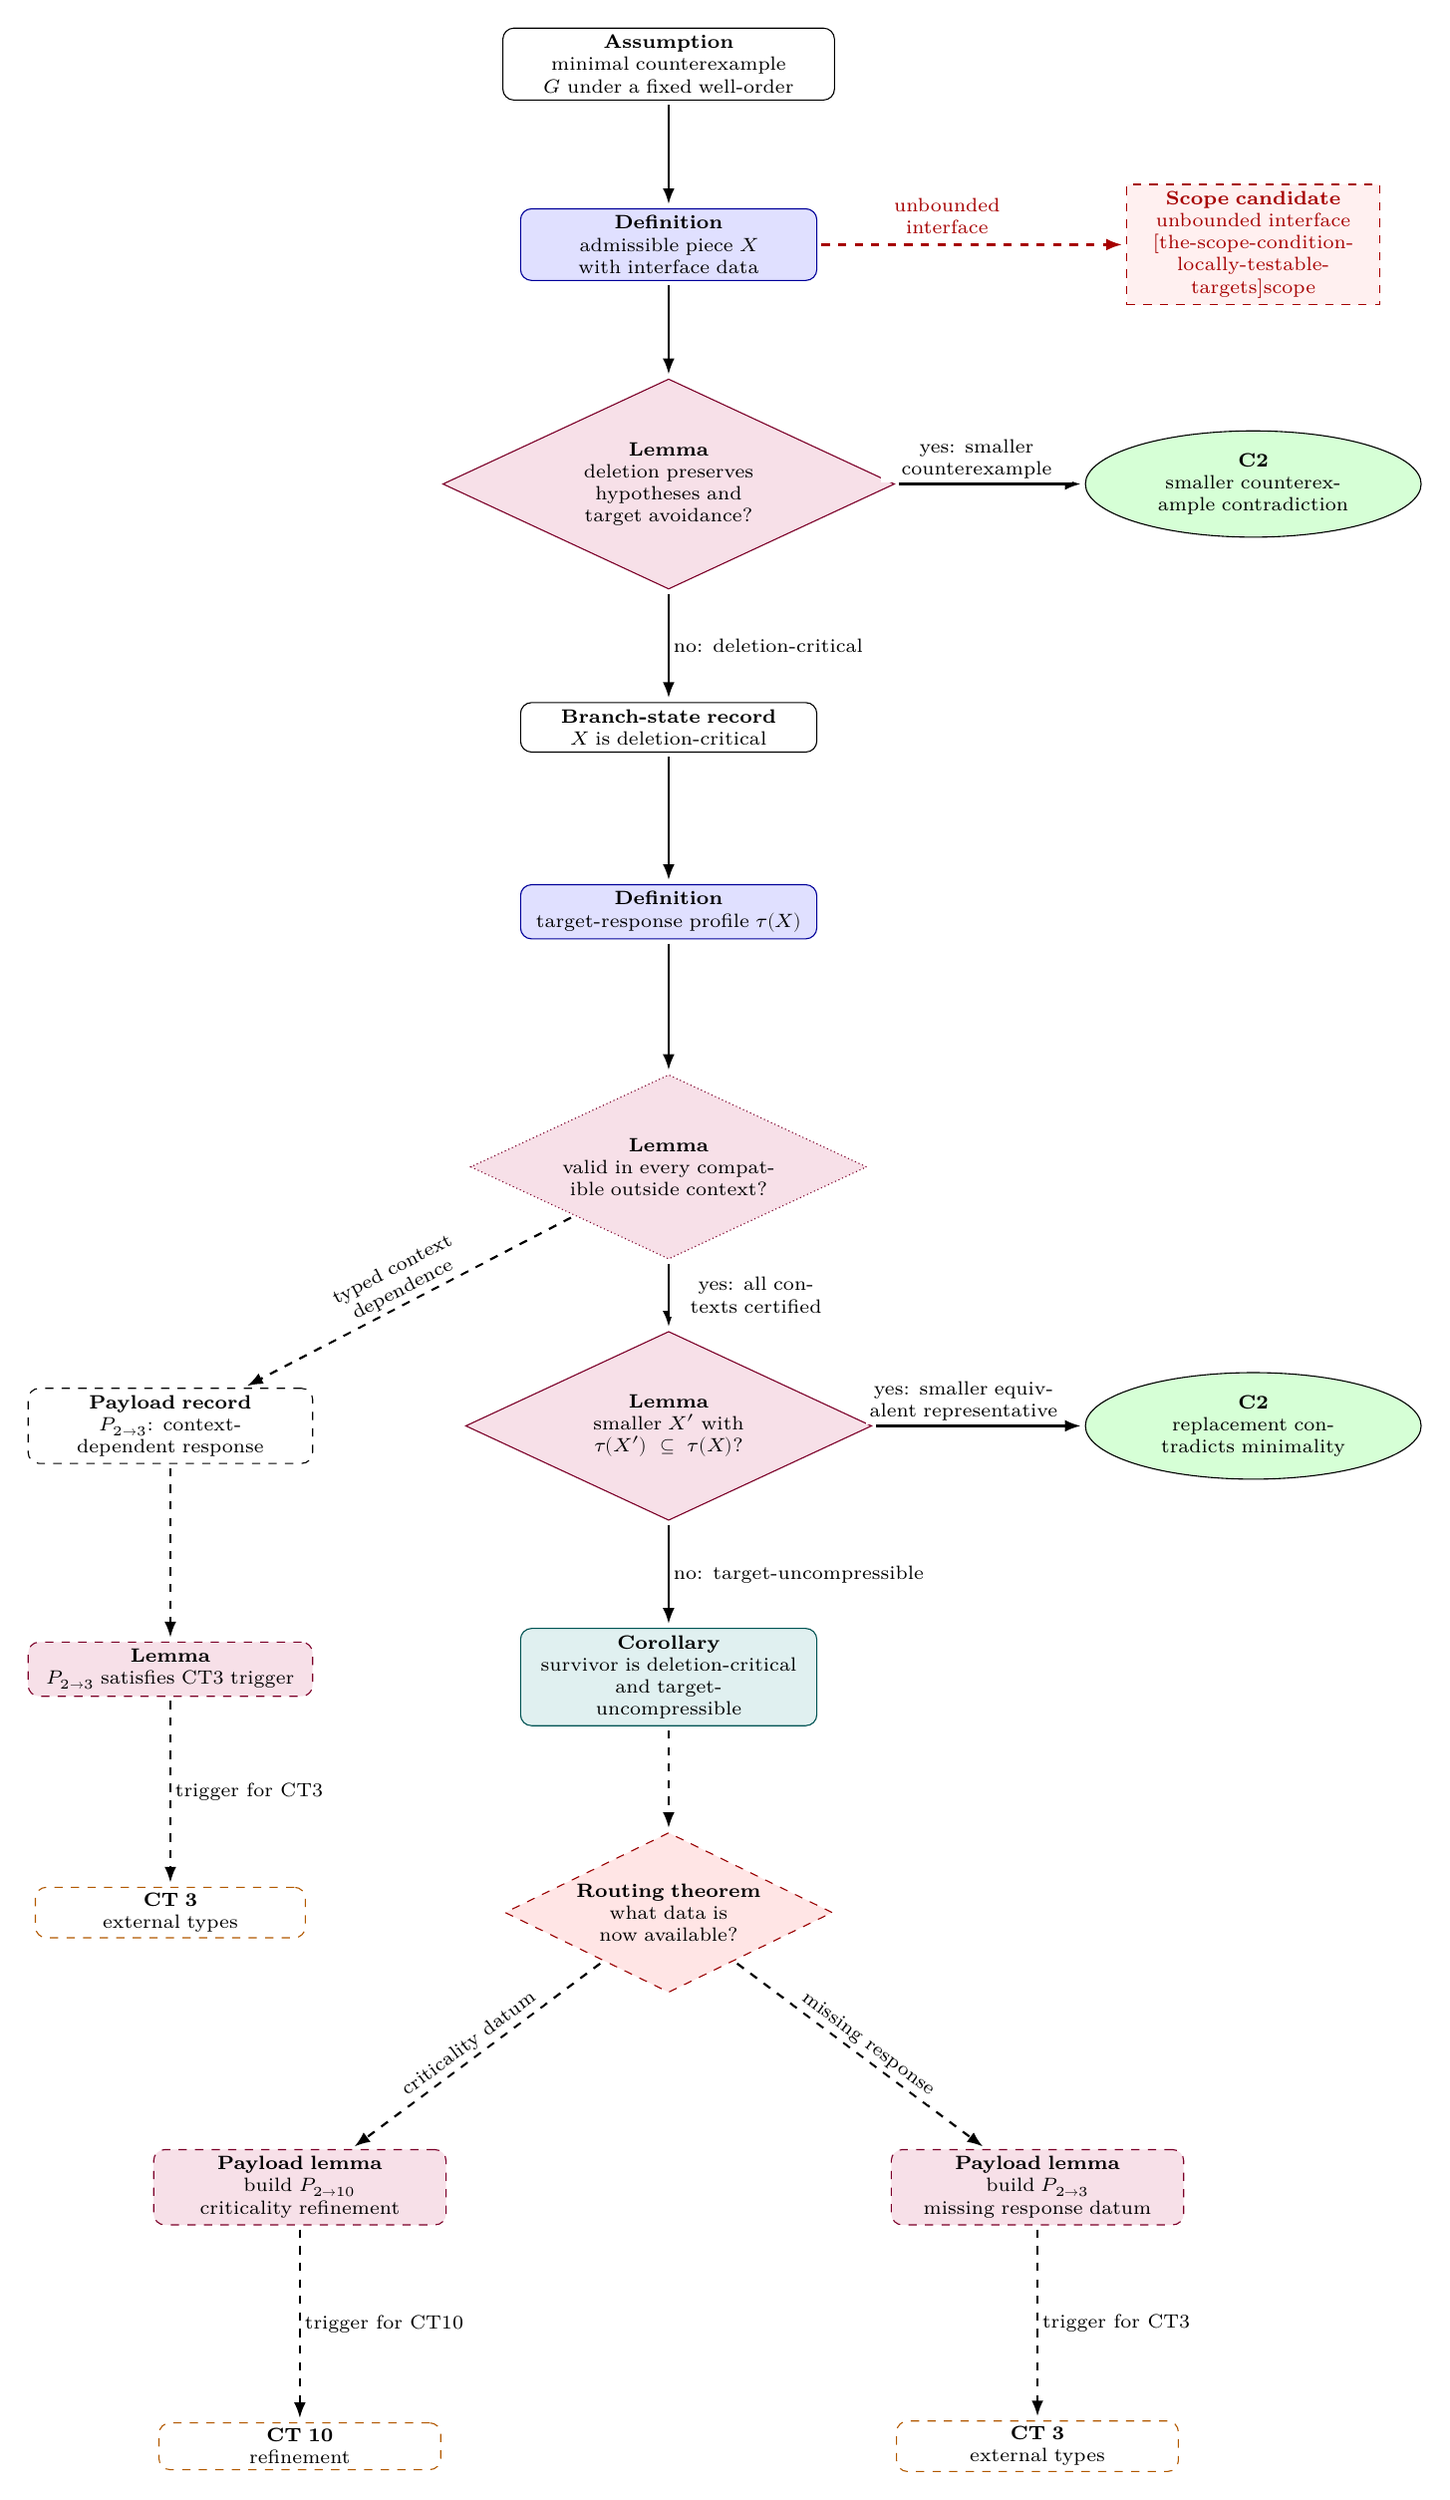
\begin{tikzpicture}[
x=1cm,
y=1cm,
every node/.style={font=\scriptsize}
]
\node[bcwide] (input) at (0,0) {\textbf{Assumption}\\minimal counterexample \(G\) under a fixed well-order};
\node[bcbox,bcdefinition,text width=3.60cm,minimum width=3.60cm] (piece) at (0,-2.30) {\textbf{Definition}\\admissible piece \(X\) with interface data};
\node[bcscopefail,text width=3.05cm,minimum width=3.05cm] (scopebad) at (7.45,-2.30) {\textbf{Scope candidate}\\unbounded interface\\\scoperef};
\node[bcdec,bclemma,text width=3.25cm,minimum width=4.05cm] (delete) at (0,-5.35) {\textbf{Lemma}\\deletion preserves hypotheses and target avoidance?};
\node[bcclosed] (delout) at (7.45,-5.35) {\textbf{C2}\\smaller counterexample contradiction};
\node[bcbox,text width=3.60cm,minimum width=3.60cm] (critical) at (0,-8.45) {\textbf{Branch-state record}\\\(X\) is deletion-critical};
\node[bcbox,bcdefinition,text width=3.60cm,minimum width=3.60cm] (profile) at (0,-10.80) {\textbf{Definition}\\target-response profile \(\tau(X)\)};
\node[bcaudit,text width=3.25cm,minimum width=4.05cm] (context) at (0,-14.05) {\textbf{Lemma}\\valid in every compatible outside context?};
\node[bcdec,bclemma,text width=3.25cm,minimum width=4.05cm] (replace) at (0,-17.35) {\textbf{Lemma}\\smaller \(X'\) with \(\tau(X')\subseteq\tau(X)\)?};
\node[bcclosed] (repout) at (7.45,-17.35) {\textbf{C2}\\replacement contradicts minimality};
\node[bcbox,bcdesign,text width=3.45cm,minimum width=3.45cm] (ctxres) at (-6.35,-17.35) {\textbf{Payload record}\\\(P_{2\to3}\): context-dependent response};
\node[bcbox,bclemma,bcdesign,text width=3.45cm,minimum width=3.45cm] (ctxlemma) at (-6.35,-20.45) {\textbf{Lemma}\\\(P_{2\to3}\) satisfies CT3 trigger};
\node[bcbox,bccorollary,text width=3.60cm,minimum width=3.60cm] (uncomp) at (0,-20.55) {\textbf{Corollary}\\survivor is deletion-critical\\and target-\\uncompressible};
\node[bcroute,bcrouteneutral,bcdesign,text width=3.30cm,minimum width=3.30cm] (ctxroute) at (-6.35,-23.55) {\textbf{CT 3}\\external types};
\node[bcroutechoice,bctheorem,bcdesign] (route) at (0,-23.55) {\textbf{Routing theorem}\\what data is now available?};
\node[bcbox,bclemma,bcdesign,text width=3.55cm,minimum width=3.55cm] (critlemma) at (-4.70,-27.05) {\textbf{Payload lemma}\\build \(P_{2\to10}\)\\criticality refinement};
\node[bcbox,bclemma,bcdesign,text width=3.55cm,minimum width=3.55cm] (resplemma) at (4.70,-27.05) {\textbf{Payload lemma}\\build \(P_{2\to3}\)\\missing response datum};
\node[bcroute,bcrouteneutral,bcdesign,text width=3.45cm,minimum width=3.45cm] (next) at (-4.70,-30.35) {\textbf{CT 10}\\refinement};
\node[bcroute,bcrouteneutral,bcdesign,text width=3.45cm,minimum width=3.45cm] (typeroute) at (4.70,-30.35) {\textbf{CT 3}\\external types};
\draw[bcarr] (input)--(piece);
\draw[bcscopearr] (piece)--node[bclabel,above,pos=.42,yshift=2pt,text width=2.05cm,align=center]{unbounded interface}(scopebad);
\draw[bcarr] (piece)--(delete);
\draw[bcarr] (delete)--node[bclabel,above,pos=0.43,text width=2.35cm,align=center]{yes: smaller counterexample}(delout);
\draw[bcarr] (delete)--node[bclabel,right]{no: deletion-critical}(critical);
\draw[bcarr] (critical)--(profile);
\draw[bcarr] (profile)--(context);
\draw[bcrecoverarr] (context)--node[bclabel,above,sloped,text width=2.20cm,align=center]{typed context dependence}(ctxres);
\draw[bcrecoverarr] (ctxres)--(ctxlemma);
\draw[bcrecoverarr] (ctxlemma)--node[bclabel,right]{trigger for CT3}(ctxroute);
\draw[bcarr] (context)--node[bclabel,right,text width=2.10cm,align=center]{yes: all contexts certified}(replace);
\draw[bcarr] (replace)--node[bclabel,above,pos=0.43,text width=2.40cm,align=center]{yes: smaller equivalent representative}(repout);
\draw[bcarr] (replace)--node[bclabel,right]{no: target-uncompressible}(uncomp);
\draw[bcrecoverarr] (uncomp)--(route);
\draw[bcrecoverarr] (route)--node[bclabel,above,sloped]{criticality datum}(critlemma);
\draw[bcrecoverarr] (route)--node[bclabel,above,sloped]{missing response}(resplemma);
\draw[bcrecoverarr] (critlemma)--node[bclabel,right]{trigger for CT10}(next);
\draw[bcrecoverarr] (resplemma)--node[bclabel,right]{trigger for CT3}(typeroute);
\end{tikzpicture}%
}
\caption[Closure-tactic 2: minimality and replacement]{Closure-tactic 2 (minimality and replacement).  The diagram records the mathematical objects required for the tactic: a minimal-counterexample assumption, an admissible piece with interface data, deletion and replacement lemmas, a context-validity lemma, the corresponding minimality closures, the routed target-uncompressible branch state that survives when both lemmas fail, and payload lemmas certifying the criticality-refinement and response-defect routes.  If the context-validity lemma fails in a typed way, CT2 constructs \(P_{2\to3}\) and routes it to CT3; if minimality leaves a target-uncompressible survivor with a missing finite label, CT2 constructs \(P_{2\to10}\) and routes it to CT10.  An unbounded interface is a candidate scope obstruction referred to the global audit in \secref{the-scope-condition-locally-testable-targets}.  Line grammar (Fig.~\ref{fig:line-grammar-legend}): solid --- intended execution through the construction of the intended residual; dotted --- checks and the post-residual handoff to the consumer tactic; dashed --- design-failure recovery; red-dashed --- candidate scope obstruction referred to the global audit.}
\label{fig:ct2-minimality-replacement}
\end{figure}
\FloatBarrier

\subsection*{Minimality and replacement in practice}

Assume a \textbf{minimal counterexample} \(G\), ordered by a
lexicographic size parameter

\[
(|G|,\ \text{secondary complexity},\ \ldots).
\]

Minimality supplies two families of tools.

\emph{Deletion/criticality tools:}

\[
\begin{gathered}
\text{if deleting or simplifying } X \text{ preserves the hypotheses}\\
\text{and avoids the target, contradiction.}
\end{gathered}
\]

\emph{Replacement/compression tools:}

\[
\begin{gathered}
\text{if a proper piece } X \text{ admits a smaller}\\
\text{target-equivalent representative, contradiction.}
\end{gathered}
\]

The second family is the engine behind every ``periodicity implies
reducibility'' step. A periodic structure contributes to the proof when
it yields a smaller representative that is target-equivalent against
\emph{all} compatible outside contexts. Here an \textbf{outside context}
is any completion of the rest of \(G\) that is compatible with the
interface data of the piece under discussion. This is the same
conceptual role played by representative replacement in the
finite-integer-index and protrusion-replacement literature
\citep{bodlaender-etal-2009-meta-kernelization, kim-etal-2012-protrusion, garnero-etal-2013-explicit-kernels, jansen-wulms-2016-lower-bounds}.

The low-level diagram for CT2 is Fig.~\ref{fig:ct2-minimality-replacement};
it records the deletion, replacement, context-validity, and residual
routing obligations used by the minimal-counterexample argument.



\subsection{CT3 --- External-type compression}\label{ct:3}\label{boundaried-pieces-and-external-types}
\ctsignature{\(P_{\ast\to3}\to \ctcert{C2,C3,C5};\ \ctint{P_{3\to7},P_{3\to12},P_{3\to8}};\ \ctrec{\ctnone}\).}

You reach CT3 when a previous tactic has exposed a piece whose behavior
must be compared through an interface.  The tactic replaces informal
``same effect outside'' reasoning by an external type that can be
checked component by component.

\ctpar{Fires when}
The state contains a certified interface and a type slot for a piece or
response datum.  Entry requires the interface and the context universe to
be recorded before any comparison begins.

\ctpar{You supply}
You supply the context universe, the type evaluator, and any replacement
table.  These are synthesized by the type-generator rules of \secref{part-iii-the-strategy-manual} and
must be finite or exact in the sense of the vocabulary block.

\ctpar{Execution}
Certify type inclusion by enumerating the recorded components of
\(\tau\): target response, exit flags, compression flags, carrier data,
and defect data.  Inclusion licenses replacement and closes by
minimality.  Equality over a finite table closes by enumeration.  The
first component that fails is not prose evidence; it is assembled as the
defect payload routed out of the tactic.

\ctpar{Soundness obligations}
\begin{itemize}
\tightlist
\item \textbf{definition} is instantiated with the certified interface \(\iota\), the external-type slot \(\tau\), and the response evaluator used by the current branch state.
\item \textbf{equivalence} is instantiated with the statement that \(\tau\) decides every compatible target-relevant context for the piece under analysis.
\item \textbf{S-Pers} is instantiated with the replacement transition that preserves the residual condition and all branch-state data required downstream.
\item \textbf{composition} is instantiated with the relevant type inclusion, finite type-table exhaustion, or compression comparison.
\item \textbf{routing} is instantiated with \(P_{3\to7}\), \(P_{3\to12}\), and \(P_{3\to8}\) for exchange defects, peelable load, and long type sequences.
\item \textbf{trigger} is instantiated with the CT7, CT12, and CT8 triggers for those three outgoing payloads.
\end{itemize}

\ctpar{Routing}
Replacement closes by C2.  Exhausted finite tables close by C5.  A defect
already in a routed account closes by C3.  Otherwise CT3 emits exchange
data to CT7, peelable load to CT12, or a repeated-type sequence to CT8.

\ctpar{Limit}
CT3 is inapplicable when the interface has infinite type index. The
execution error is asserting type inclusion without checking the recorded
components; the audit records CT3/equivalence or CT3/routing.

\begin{figure}[p]
\centering
\vspace*{-2.80cm}
\resizebox{!}{0.72\textheight}{%
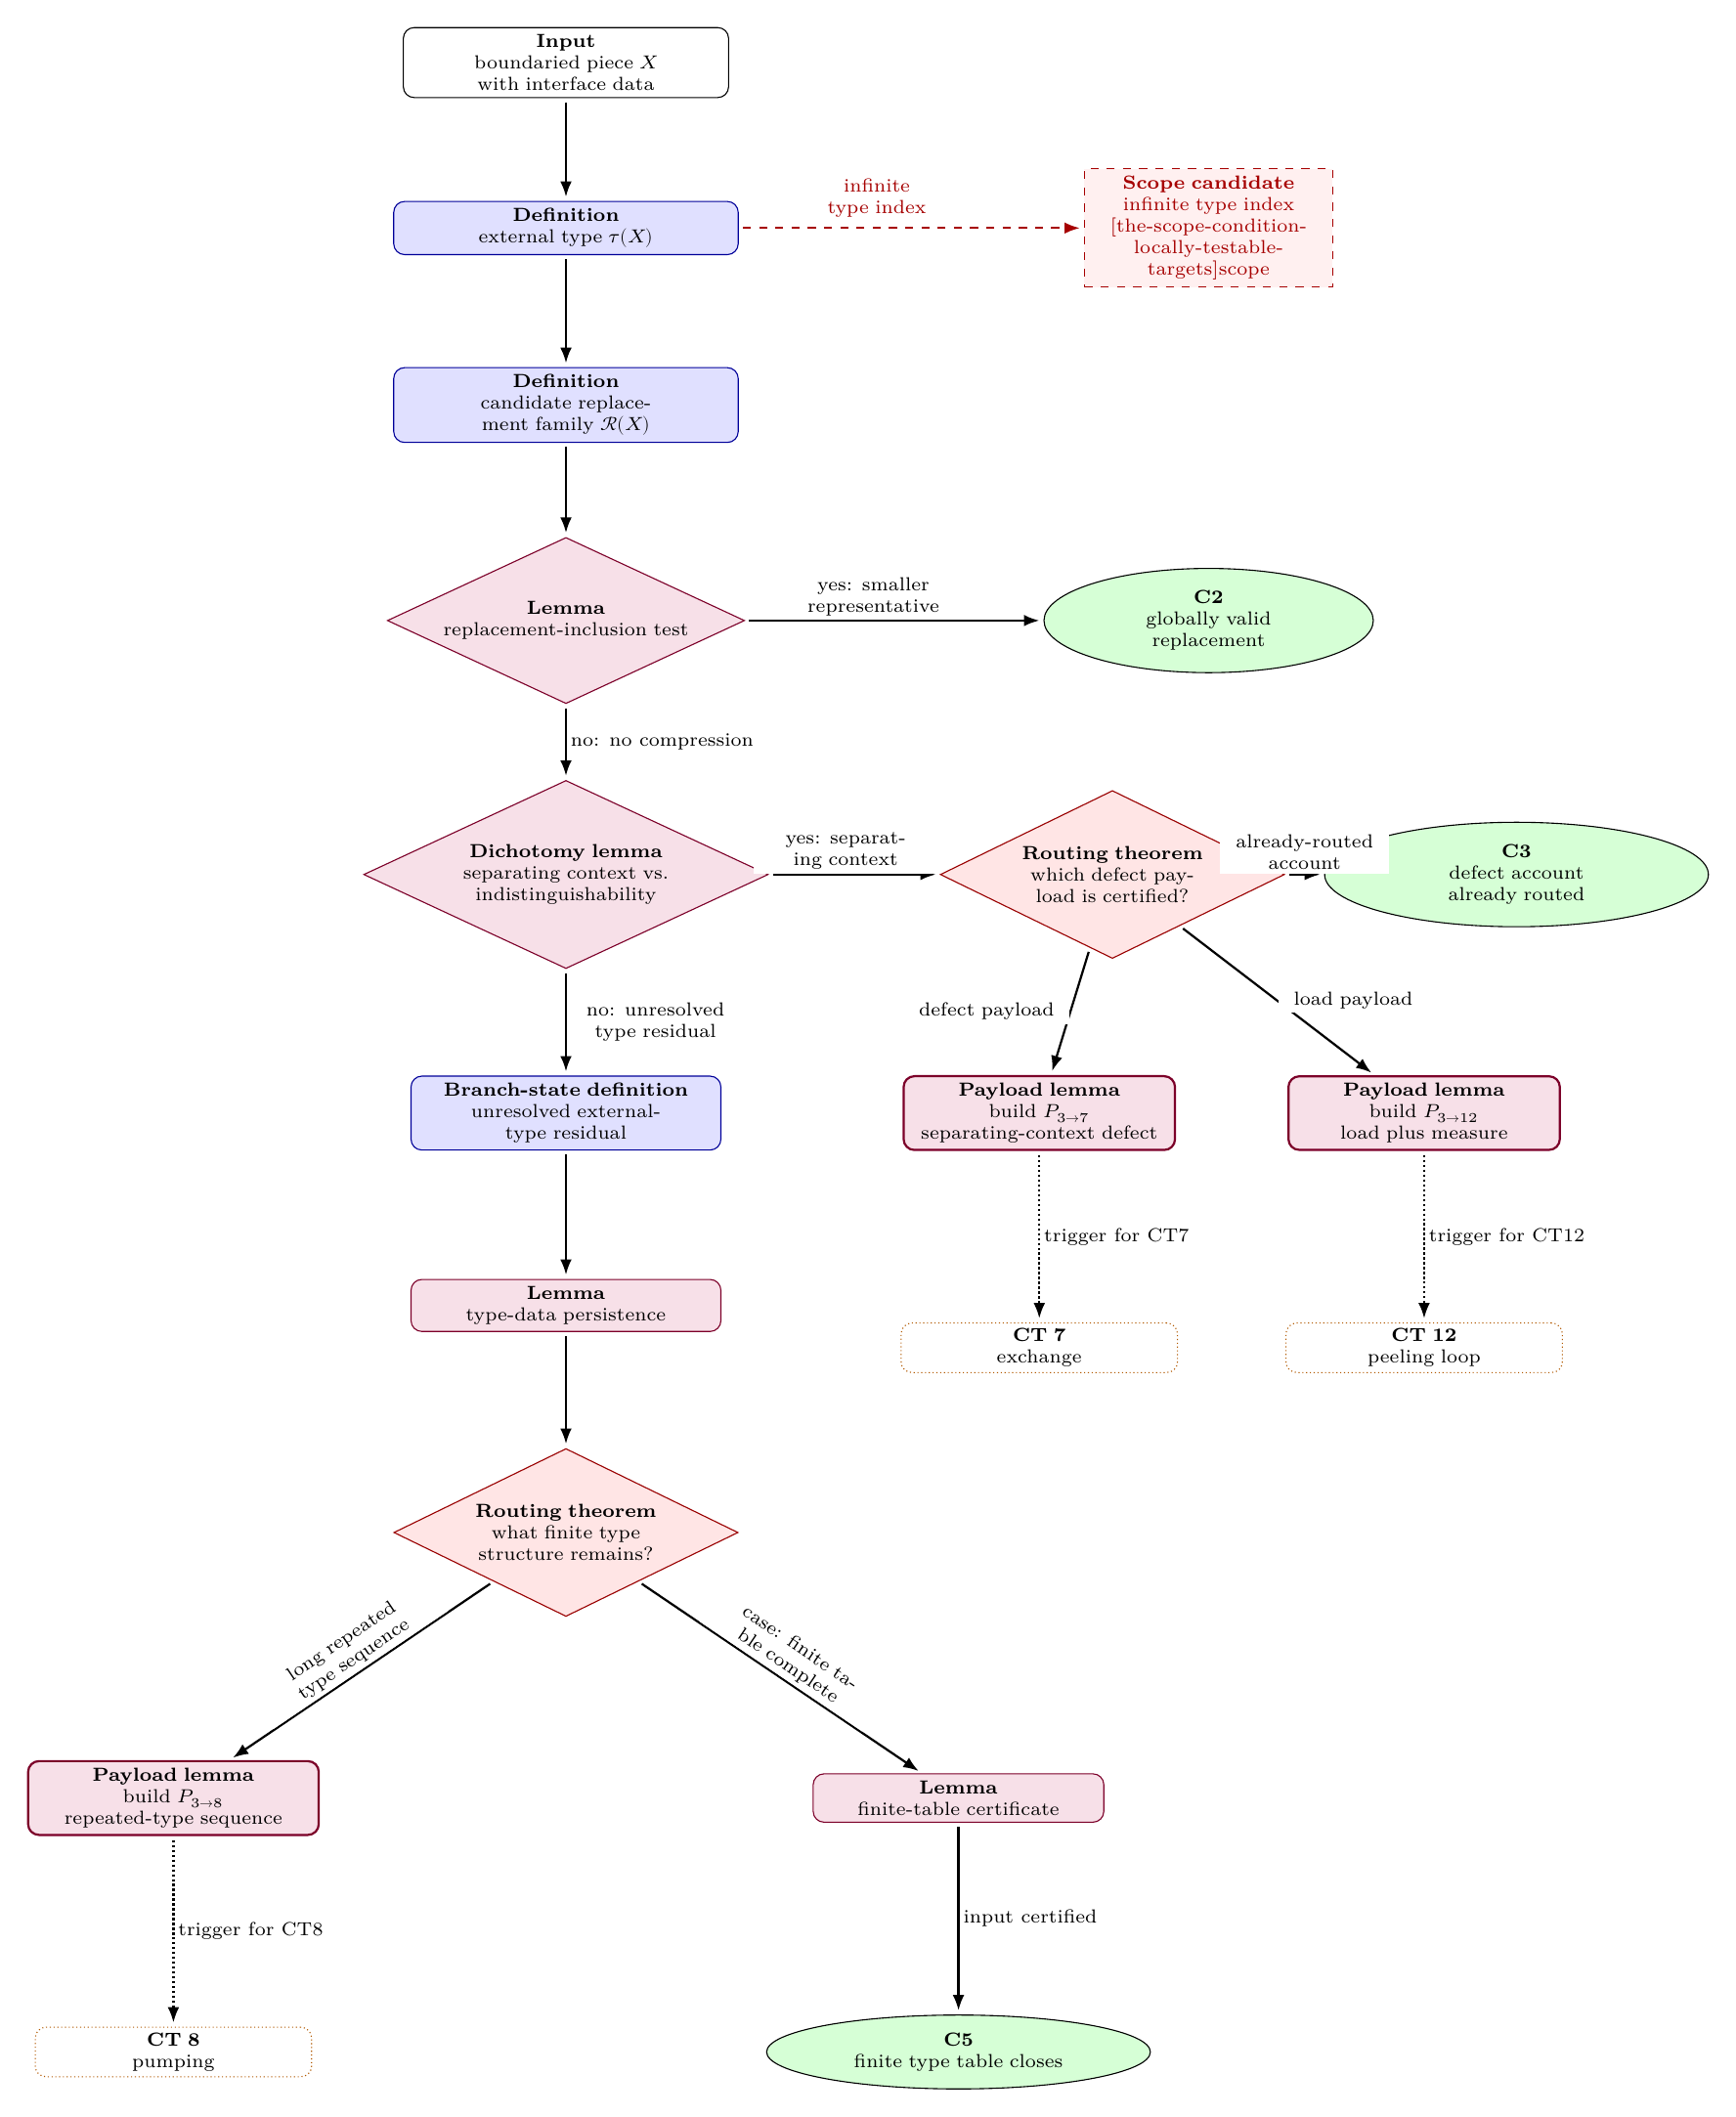
\begin{tikzpicture}[
x=1cm,
y=1cm,
every node/.style={font=\scriptsize}
]
\node[bcwide] (piece) at (0,0) {\textbf{Input}\\boundaried piece \(X\) with interface data};
\node[bcwide,bcdefinition,text width=4.30cm,minimum width=4.30cm] (type) at (0,-2.15) {\textbf{Definition}\\external type \(\tau(X)\)};
\node[bcscopefail,text width=3.05cm,minimum width=3.05cm] (scopebad) at (8.35,-2.15) {\textbf{Scope candidate}\\infinite type index\\\scoperef};
\node[bcwide,bcdefinition,text width=4.30cm,minimum width=4.30cm] (replacements) at (0,-4.45) {\textbf{Definition}\\candidate replacement family \(\mathcal R(X)\)};
\node[bcdec,bclemma,text width=3.35cm,minimum width=4.15cm] (compare) at (0,-7.25) {\textbf{Lemma}\\replacement-inclusion test};
\node[bcclosed] (compress) at (8.35,-7.25) {\textbf{C2}\\globally valid replacement};
\node[bcdec,bclemma,text width=3.35cm,minimum width=4.15cm] (distinguish) at (0,-10.55) {\textbf{Dichotomy lemma}\\separating context vs.\ indistinguishability};
\node[bcroutechoice,bctheorem,text width=2.75cm,minimum width=3.35cm] (defectlemma) at (7.10,-10.55) {\textbf{Routing theorem}\\which defect payload is certified?};
\node[bcclosed,text width=3.35cm,minimum width=3.35cm] (routedclose) at (12.35,-10.55) {\textbf{C3}\\defect account already routed};
\node[bcbox,bclemma,bcpayload,text width=3.35cm,minimum width=3.35cm] (exchlemma) at (6.15,-13.65) {\textbf{Payload lemma}\\build \(P_{3\to7}\)\\separating-context defect};
\node[bcroute,bcrouteneutral,bcoutputroute,text width=3.45cm,minimum width=3.45cm] (defect) at (6.15,-16.70) {\textbf{CT 7}\\exchange};
\node[bcbox,bclemma,bcpayload,text width=3.35cm,minimum width=3.35cm] (peellemma) at (11.15,-13.65) {\textbf{Payload lemma}\\build \(P_{3\to12}\)\\load plus measure};
\node[bcroute,bcrouteneutral,bcoutputroute,text width=3.45cm,minimum width=3.45cm] (peelroute) at (11.15,-16.70) {\textbf{CT 12}\\peeling loop};
\node[bcbox,bcdefinition,text width=3.85cm,minimum width=3.85cm] (residual) at (0,-13.65) {\textbf{Branch-state definition}\\unresolved external-type residual};
\node[bcbox,bclemma,text width=3.85cm,minimum width=3.85cm] (persist) at (0,-16.15) {\textbf{Lemma}\\type-data persistence};
\node[bcroutechoice,bctheorem,text width=2.75cm,minimum width=3.35cm] (next) at (0,-19.10) {\textbf{Routing theorem}\\what finite type structure remains?};
\node[bcbox,bclemma,bcpayload,text width=3.60cm,minimum width=3.60cm] (repeatlemma) at (-5.10,-22.55) {\textbf{Payload lemma}\\build \(P_{3\to8}\)\\repeated-type sequence};
\node[bcbox,bclemma,text width=3.60cm,minimum width=3.60cm] (tablelemma) at (5.10,-22.55) {\textbf{Lemma}\\finite-table certificate};
\node[bcroute,bcrouteneutral,bcoutputroute,text width=3.45cm,minimum width=3.45cm] (pumproute) at (-5.10,-25.85) {\textbf{CT 8}\\pumping};
\node[bcclosed,text width=3.35cm,minimum width=3.35cm] (tableclose) at (5.10,-25.85) {\textbf{C5}\\finite type table closes};
\draw[bcarr] (piece)--(type);
\draw[bcscopearr] (type)--node[bclabel,above,pos=.40,yshift=2pt,text width=2.10cm,align=center]{infinite type index}(scopebad);
\draw[bcarr] (type)--(replacements);
\draw[bcarr] (replacements)--(compare);
\draw[bcarr] (compare)--node[bclabel,above,pos=0.43,text width=2.40cm,align=center]{yes: smaller representative}(compress);
\draw[bcarr] (compare)--node[bclabel,right]{no: no compression}(distinguish);
\draw[bcarr] (distinguish)--node[bclabel,above,pos=0.45,text width=2.30cm,align=center]{yes: separating context}(defectlemma);
\draw[bcarr] (defectlemma)--node[bclabel,above,text width=2.10cm,align=center]{already-routed account}(routedclose);
\draw[bcarr] (defectlemma)--node[bclabel,left,text width=2.05cm,align=center]{defect payload}(exchlemma);
\draw[bcarr] (defectlemma)--node[bclabel,right,text width=1.85cm,align=center]{load payload}(peellemma);
\draw[bchandoff] (exchlemma)--node[bclabel,right]{trigger for CT7}(defect);
\draw[bchandoff] (peellemma)--node[bclabel,right]{trigger for CT12}(peelroute);
\draw[bcarr] (distinguish)--node[bclabel,right,text width=2.20cm,align=center]{no: unresolved type residual}(residual);
\draw[bcarr] (residual)--(persist);
\draw[bcarr] (persist)--(next);
\draw[bcarr] (next)--node[bclabel,above,sloped,text width=2.65cm,align=center]{long repeated type sequence}(repeatlemma);
\draw[bcarr] (next)--node[bclabel,above,sloped,text width=2.45cm,align=center]{case: finite table complete}(tablelemma);
\draw[bchandoff] (repeatlemma)--node[bclabel,right]{trigger for CT8}(pumproute);
\draw[bcarr] (tablelemma)--node[bclabel,right]{input certified}(tableclose);
\end{tikzpicture}%
}
\caption[Closure-tactic 3: external-type compression]{Closure-tactic 3 (external-type compression).  The diagram records the objects needed to make external-type compression airtight: the external-type definition, replacement-family definition, replacement-inclusion lemma, separating-context dichotomy, residual branch-state definition, persistence lemma, routing theorem, and payload lemmas certifying defect routing, peelable defect-load routing with a well-founded measure, pumping, or finite-table closure.  Its terminal exits are C2 (replacement), C3 (an accepted routed-defect account), and C5 (finite-table exhaustion); its typed exits are \(P_{3\to7}\) for a separating-context defect, \(P_{3\to12}\) for a routed load with measure, and \(P_{3\to8}\) for a long repeated-type sequence.  equivalence must certify the recorded profile before comparison begins; infinite type index is a candidate scope obstruction referred to the global audit in \secref{the-scope-condition-locally-testable-targets}.  Line grammar (Fig.~\ref{fig:line-grammar-legend}): solid --- intended execution through the construction of the intended residual; dotted --- checks and the post-residual handoff to the consumer tactic; dashed --- design-failure recovery; red-dashed --- candidate scope obstruction referred to the global audit.}
\label{fig:ct3-external-type-compression}
\end{figure}
\FloatBarrier

\subsection*{External-type compression in practice}

A piece \(X\) is analyzed as a boundaried piece
\((X,\partial X,\text{interface data})\). To each piece one attaches its
\textbf{external type}

\[
\begin{aligned}
\tau(X) \;={}& \text{all target-relevant answers that } X\\
&\text{ can exhibit to compatible outside contexts}.
\end{aligned}
\]

Two pieces have the same external type when no admissible context can
distinguish them with respect to the target. This is a Myhill--Nerode-style
context equivalence, analogous to a type in logic and to the
graph-theoretic analogue of the context-equivalence viewpoint in
Courcelle-style recognizability and boundaried-graph replacement
\citep{myhill-1957-automata, nerode-1958-linear, courcelle-1990-mso-graphs, courcelle-engelfriet-2012-graph-structure, bodlaender-etal-2009-meta-kernelization}.

An external type typically records boundary degrees, attachment order,
local labels, and the responses of the local tests restricted to \(X\).
It also records \textbf{exit flags}, compression flags, and carrier
data. An exit flag is a bit recording which named closure routes of
\secref{the-branch-taxonomy} remain available in the current branch state. A
\textbf{carrier} is an auxiliary bounded substructure, canonically
associated to \(X\), that carries interface and target data between
distant pieces and to which charges may later be routed.

A smaller piece \(X'\) may replace \(X\) only if

\[
\tau(X') \subseteq \tau(X)
\]

(or with equality, depending on the replacement lemma in force). This
inclusion is what converts a local reduction into a globally valid one.

The low-level diagram for CT3 is Fig.~\ref{fig:ct3-external-type-compression};
it spells out the external-type definition, replacement test,
separating-context branch, and typed exits.



\subsection{CT4 --- Charging schemes}\label{ct:4}\label{charging-schemes}
\ctsignature{\(P_{\ast\to4}\to \ctcert{C4};\ \ctint{P_{4\to9},P_{4\to14}};\ \ctrec{P_{4\to13}}\).}

You reach CT4 when the branch state already contains a demand/payer
account, often emitted by CT1, CT5, CT6, CT9, CT12, CT13, or CT15.  The
tactic turns that ledger into a capacity contradiction or a named
capacity residual.

\ctpar{Fires when}
The state records a demand set \(\mathcal D\), payer set \(\mathcal P\),
proposed canonical assignment rule \(\pi\), capacity bound \(C\), and
lower-bound target \(\ell\).  Entry is permitted only after these ledger
data exist in the vocabulary record; totality of \(\pi\) is established
during execution.

\ctpar{You supply}
You supply the canonical assignment rule, its tie-breaking rule, the capacity
proof, and the lower-bound estimate.  \secref{part-iii-the-strategy-manual} synthesizes the payer
inventory and rate data; CT4 only checks the ledger it receives.

\ctpar{Execution}
Build the ledger in the fixed order: define demands, define payers,
define the canonical assignment rule with explicit tie-breaking, prove
that it is total, defer bounded
multiplicity to CT9, and prove the capacity inequality.  The deferral is
part of the tactic: no-overcount is established by exhausting the
overloaded fibre, not by assuming the map is nearly injective.  A demand
with no available payer is recorded with its availability obstruction
and packaged as \(P_{4\to13}\).

\ctpar{Soundness obligations}
\begin{itemize}
\tightlist
\item \textbf{definition} is instantiated with the demand set \(\mathcal D\), payer set \(\mathcal P\), charge map \(\pi\), capacity data, and lower-bound target.
\item \textbf{S-Det} is instantiated with the canonical definition of \(\pi\), including every tie-break used to choose a payer.
\item \textbf{dichotomy} is instantiated with the alternatives that certified capacity closes the branch or an overload fibre remains.
\item \textbf{composition} is instantiated with the bounded-capacity inequality comparing total demand with available payer capacity.
\item \textbf{routing} is instantiated with \(P_{4\to9}\) for an overcharged fibre, \(P_{4\to14}\) for aggregate residual mass, and \(P_{4\to13}\) for a demand with no available payer.
\item \textbf{trigger} is instantiated with the CT9 trigger for overload data, the CT14 trigger for aggregate mass data, and the CT13 trigger for a tier-interaction obstruction.
\end{itemize}

\ctpar{Routing}
If demand exceeds certified capacity, CT4 closes by C4.  An overcharged
fibre emits \(P_{4\to9}\) to CT9.  A residual class carrying mass beyond
the pointwise ledger emits \(P_{4\to14}\) to CT14.  A demand with no
available payer emits \(P_{4\to13}\) to CT13.

\ctpar{Limit}
CT4 is inapplicable when the branch state contains no admissible locally
generated demand family. The
execution error is a nondeterministic charge map; the audit records
CT4/S-Det and rejects the ledger until the tie-breaking rule is part of
the branch state.

\begin{figure}[p]
\centering
\vspace*{-2.80cm}
\resizebox{0.88\textwidth}{!}{%
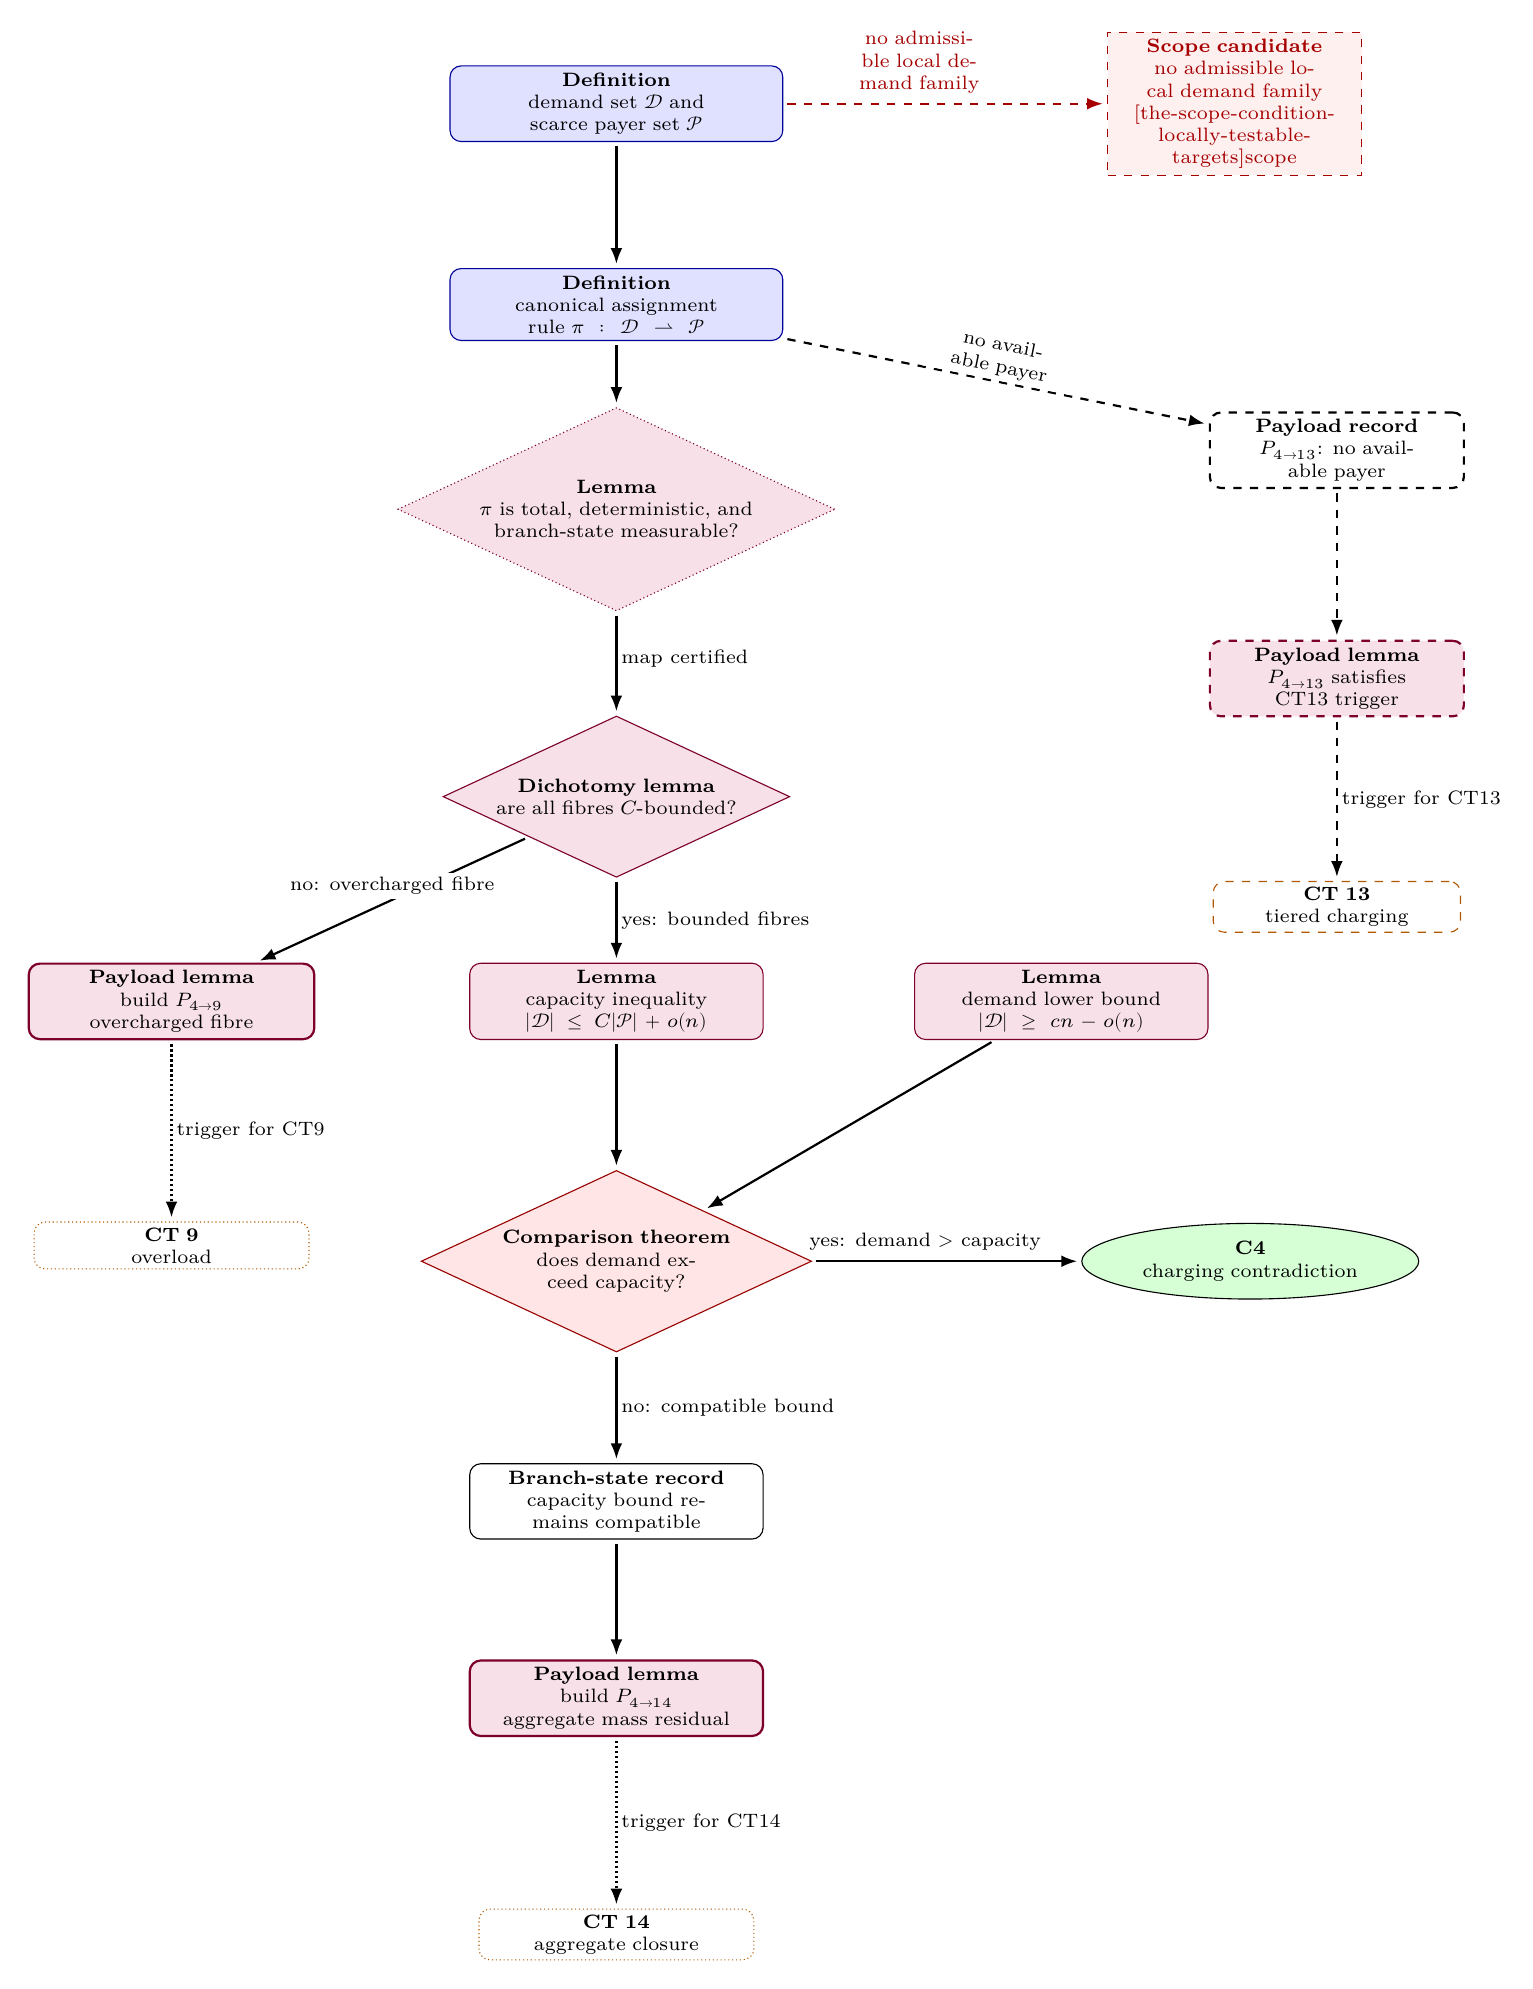
\begin{tikzpicture}[
every node/.style={font=\scriptsize}
]
\node[bcwide,bcdefinition] (input) at (0,0.70) {\textbf{Definition}\\demand set \(\mathcal D\) and scarce payer set \(\mathcal P\)};
\node[bcscopefail,text width=3.05cm,minimum width=3.05cm] (scopebad) at (7.85,0.70) {\textbf{Scope candidate}\\no admissible local demand family\\\scoperef};
\node[bcwide,bcdefinition] (assign) at (0,-1.85) {\textbf{Definition}\\canonical assignment rule \(\pi:\mathcal D\rightharpoonup\mathcal P\)};
\node[bcbox,bcdesign,bcpayload,text width=3.05cm,minimum width=3.05cm] (nopayer) at (9.15,-3.70) {\textbf{Payload record}\\\(P_{4\to13}\): no available payer};
\node[bcbox,bclemma,bcdesign,bcpayload,text width=3.05cm,minimum width=3.05cm] (tierrepair) at (9.15,-6.60) {\textbf{Payload lemma}\\\(P_{4\to13}\) satisfies CT13 trigger};
\node[bcroute,bcrouteneutral,bcdesign,text width=3.00cm,minimum width=3.00cm] (tierroute) at (9.15,-9.50) {\textbf{CT 13}\\tiered charging};
\node[bcauditbox,text width=3.75cm,minimum width=3.75cm] (canon) at (0,-4.45) {\textbf{Lemma}\\\(\pi\) is total, deterministic, and branch-state measurable?};
\node[bcdec,bclemma,text width=3.20cm,minimum width=4.00cm] (mult) at (0,-8.10) {\textbf{Dichotomy lemma}\\are all fibres \(C\)-bounded?};
\node[bcbox,bclemma,bcpayload,text width=3.45cm,minimum width=3.45cm] (overtrig) at (-5.65,-10.70) {\textbf{Payload lemma}\\build \(P_{4\to9}\)\\overcharged fibre};
\node[bcroute,bcrouteneutral,bcoutputroute,text width=3.35cm,minimum width=3.35cm] (overload) at (-5.65,-13.80) {\textbf{CT 9}\\overload};
\node[bcbox,bclemma,text width=3.55cm,minimum width=3.55cm] (cap) at (0,-10.70) {\textbf{Lemma}\\capacity inequality\\\(|\mathcal D|\le C|\mathcal P|+o(n)\)};
\node[bcbox,bclemma,text width=3.55cm,minimum width=3.55cm] (lower) at (5.65,-10.70) {\textbf{Lemma}\\demand lower bound\\\(|\mathcal D|\ge cn-o(n)\)};
\node[bcdec,bctheorem,text width=3.05cm,minimum width=3.90cm] (contr) at (0,-14.00) {\textbf{Comparison theorem}\\does demand exceed capacity?};
\node[bcclosed] (out) at (8.05,-14.00) {\textbf{C4}\\charging contradiction};
\node[bcbox,text width=3.55cm,minimum width=3.55cm] (open) at (0,-17.05) {\textbf{Branch-state record}\\capacity bound remains compatible};
\node[bcbox,bclemma,bcpayload,text width=3.55cm,minimum width=3.55cm] (masslemma) at (0,-19.55) {\textbf{Payload lemma}\\build \(P_{4\to14}\)\\aggregate mass residual};
\node[bcroute,bcrouteneutral,bcoutputroute,text width=3.35cm,minimum width=3.35cm] (aggregate) at (0,-22.55) {\textbf{CT 14}\\aggregate closure};
\draw[bcscopearr] (input)--node[bclabel,above,pos=.42,yshift=2pt,text width=2.20cm,align=center]{no admissible local demand family}(scopebad);
\draw[bcarr] (input)--(assign);
\draw[bcrecoverarr] (assign)--node[bclabel,above,sloped,text width=1.85cm,align=center]{no available payer}(nopayer);
\draw[bcrecoverarr] (nopayer)--(tierrepair);
\draw[bcrecoverarr] (tierrepair)--node[bclabel,right]{trigger for CT13}(tierroute);
\draw[bcarr] (assign)--(canon);
\draw[bcarr] (canon)--node[bclabel,right,pos=.45]{map certified}(mult);
\draw[bcarr] (mult)--node[bclabel,above]{no: overcharged fibre}(overtrig);
\draw[bchandoff] (overtrig)--node[bclabel,right]{trigger for CT9}(overload);
\draw[bcarr] (mult)--node[bclabel,right]{yes: bounded fibres}(cap);
\draw[bcarr] (lower)--(contr);
\draw[bcarr] (cap)--(contr);
\draw[bcarr] (contr)--node[bclabel,above,pos=.42,yshift=2pt]{yes: demand \(>\) capacity}(out);
\draw[bcarr] (contr)--node[bclabel,right]{no: compatible bound}(open);
\draw[bcarr] (open)--(masslemma);
\draw[bchandoff] (masslemma)--node[bclabel,right]{trigger for CT14}(aggregate);
\end{tikzpicture}%
}
\caption[Closure-tactic 4: charging schemes]{Closure-tactic 4 (charging schemes).  The tactic is certified by definitions of the demand set, payer set, and canonical charge map; a determinism lemma; a bounded-fibre dichotomy lemma; capacity and demand lower-bound lemmas; and a comparison theorem that either closes the branch or routes a typed residual.  An overcharged fibre is packaged as \(P_{4\to9}\) and consumed by CT9; a compatible but unresolved aggregate mass account is packaged as \(P_{4\to14}\) and consumed by CT14.  A demand with no available payer constructs the recovery payload \(P_{4\to13}\) for CT13; absence of an admissible locally generated demand family is a candidate scope obstruction referred to the global audit in \secref{the-scope-condition-locally-testable-targets}.  Line grammar (Fig.~\ref{fig:line-grammar-legend}): solid --- intended execution through the construction of the intended residual; dotted --- checks and the post-residual handoff to the consumer tactic; dashed --- design-failure recovery; red-dashed --- candidate scope obstruction referred to the global audit.}
\label{fig:ct4-charging-schemes}
\end{figure}
\FloatBarrier

\subsection*{Charging schemes in practice}

A \textbf{charging scheme} is an injective or bounded-multiplicity
assignment from \textbf{demands} --- the events that must be accounted
for --- to \textbf{payers} --- the scarce structures that absorb the
charges. A payer that has absorbed its full capacity is
\textbf{saturated}. This is the same mechanism as the classical charging
and discharging arguments, packaged with an explicit interface. The
reference class is the discharging/reducibility architecture of the
four-colour theorem and its later expositions
\citep{appel-haken-1977-discharging, appel-haken-koch-1977-reducibility, robertson-etal-1997-four-colour, cranston-west-2017-discharging}.

A charging scheme has four parts.

\begin{enumerate}
\def\labelenumi{\arabic{enumi}.}
\tightlist
\item
  \textbf{Demand definition.} This specifies what must be paid for.
  Typical demands are bad \textbf{windows}, blocked pairs, missing
  attachment points, \textbf{route entries}, saturated payers, and
  first-failure witnesses (\secref{the-activedormant-dichotomy}). A \emph{window} is a bounded-size
  region of \(G\), fixed by the local structure of the branch, inside
  which the local tests are evaluated; it is \emph{bad} if the required
  tests fail there. A route entry is a record deposited in the charging
  scheme of a previously named branch; see ``routed'' in \secref{the-branch-taxonomy}.
\item
  \textbf{Canonical assignment.} Each demand selects one canonical payer
  under an explicit deterministic tie-break. This makes the ledger
  auditable. The bounded-multiplicity lemma, not determinism, controls how
  many demands may select the same payer.
\item
  \textbf{Bounded-multiplicity lemma} (the \emph{no-overcount} lemma).
  Each payer is charged at most \(C\) times --- or else an
  already-routed branch occurs (\secref{the-charging-principle-in-general-form}).
\item
  \textbf{Capacity inequality.} \[
  |\mathcal D| \;\le\; C\,|\mathcal P| + o(n).
  \]
\end{enumerate}

When the proof requires a contradiction, the capacity inequality is
combined with a demand lower bound \(|\mathcal D|\ge cn - o(n)\); the
contradiction \(cn \le C|\mathcal P| + o(n)\) closes the branch whenever
the payers are known to number \(o(n)\) or to lie below threshold.

The low-level diagram for CT4 is Fig.~\ref{fig:ct4-charging-schemes};
it shows where the demand, payer, canonical map, bounded-fibre lemma,
capacity comparison, and routed residual payloads enter.


\subsection{CT5 --- Local-to-global bookkeeping}\label{ct:5}\label{the-local-versus-global-rationale}
\ctsignature{\(P_{1\to5}\to \ctcert{C4};\ \ctint{P_{5\to4},P_{5\to11},P_{5\to14}};\ \ctrec{\ctnone}\).}

You reach CT5 when CT1 has produced a linear local-site family.  The
tactic turns many local witnesses into a global comparison by proving
each local arrow separately before summing.

\ctpar{Fires when}
The state contains a linear family \(\mathcal S\), site labels, a witness
extractor, and a locality record.

\ctpar{You supply}
You supply the local lower bound, the site labels, and the summation
domain.  These are synthesized by the invariant, label, and budget rules
of \secref{part-iii-the-strategy-manual}.

\ctpar{Execution}
Implement the four-arrow chain as four lemmas: local tests define local
demands; absent tests create bounded local witnesses; witnesses map to
scarce payers; and the local inequalities sum to the global capacity
comparison.  The global estimate is assembled only after every arrow has
its own lemma.

\ctpar{Soundness obligations}
\begin{itemize}
\tightlist
\item \textbf{definition} is instantiated with the local-site family \(\mathcal S\), its site labels, the witness extractor, and the locality record.
\item \textbf{S-Det} is instantiated with the canonical site-to-payer assignment used when local witnesses form a charge map.
\item \textbf{composition} is instantiated with the local-to-global summation and the resulting global capacity comparison.
\item \textbf{routing} is instantiated with \(P_{5\to4}\), \(P_{5\to11}\), and \(P_{5\to14}\) for charge ledgers, additive deficits, and local-mass shortfalls.
\item \textbf{trigger} is instantiated with the CT4, CT11, and CT14 triggers for the outgoing local-to-global payloads.
\end{itemize}

\ctpar{Routing}
A completed comparison closes by C4.  A local charge ledger routes to
CT4, an additive global deficit routes to CT11, and a local-mass
shortfall routes to CT14.

\ctpar{Limit}
CT5 is inapplicable when no bounded local witnesses are available. The
execution error is a missing locality lemma; the audit records CT5/definition
or CT5/composition.

\begin{figure}[p]
\centering
\vspace*{-2.80cm}
\resizebox{\textwidth}{!}{%
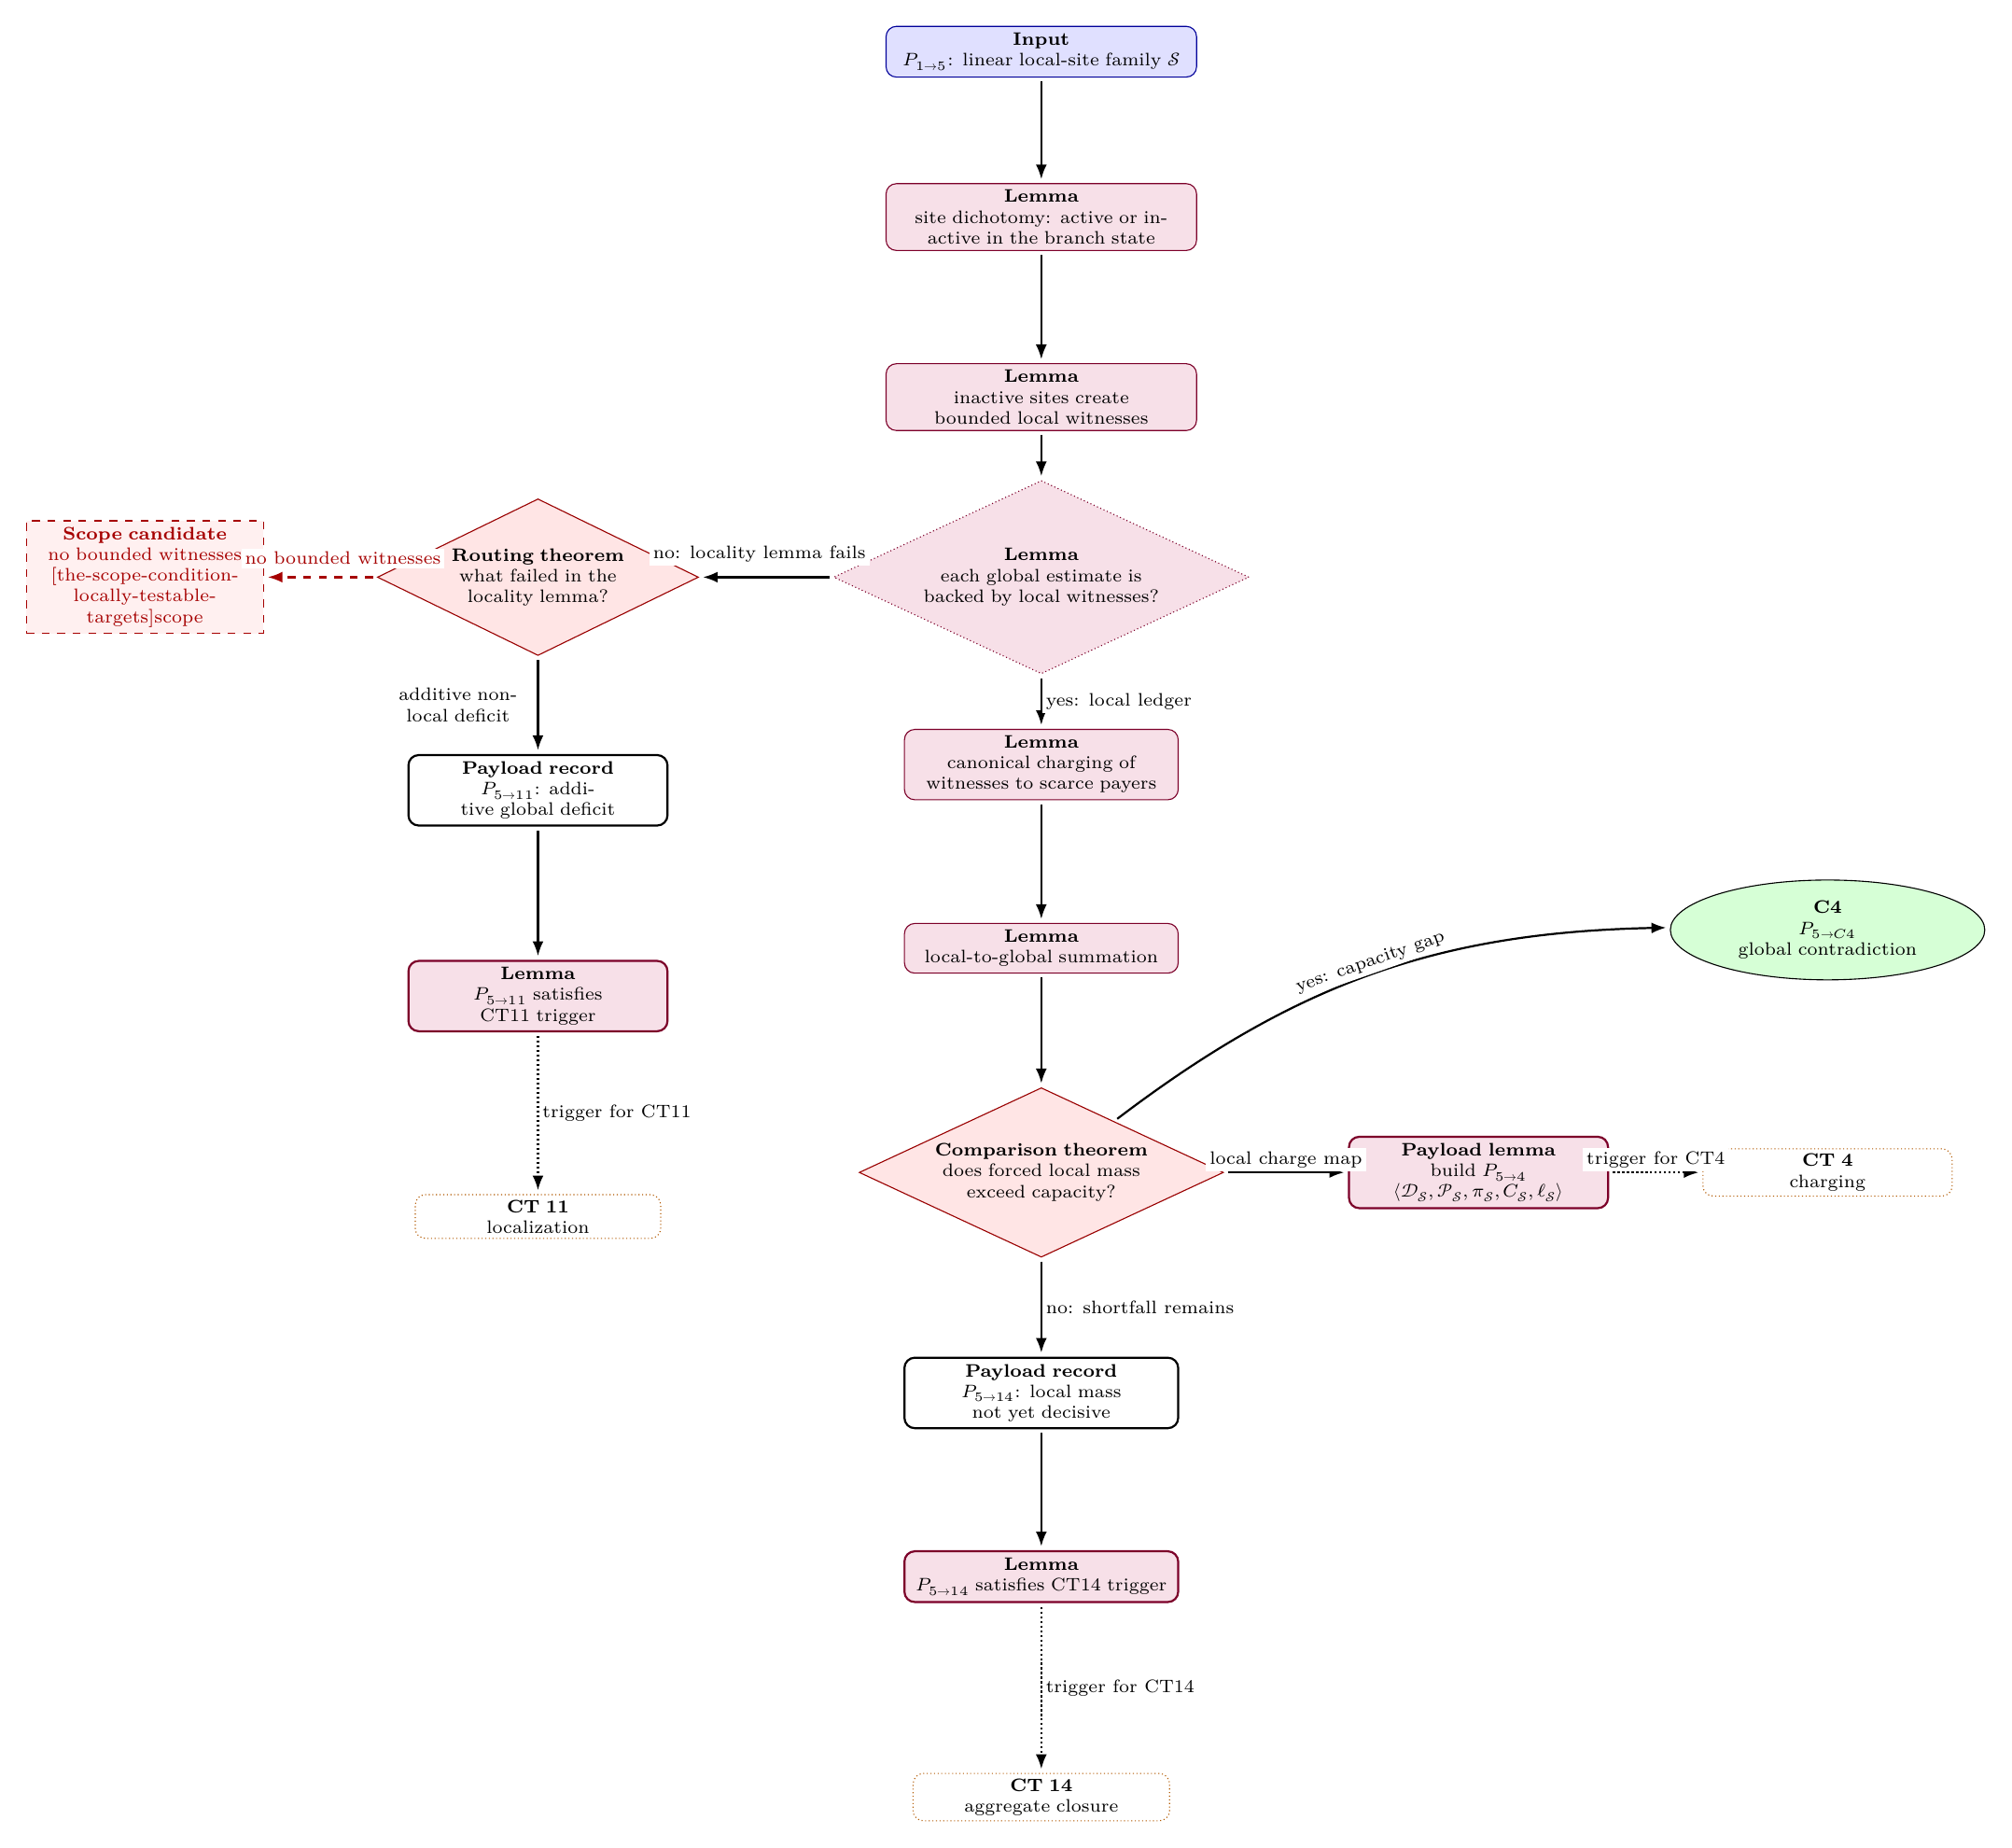
\begin{tikzpicture}[
every node/.style={font=\scriptsize}
]
\node[bcwide,bcdefinition] (input) at (0,0) {\textbf{Input}\\\(P_{1\to5}\): linear local-site family \(\mathcal S\)};
\node[bcwide,bclemma] (tests) at (0,-2.25) {\textbf{Lemma}\\site dichotomy: active or inactive in the branch state};
\node[bcwide,bclemma] (demands) at (0,-4.70) {\textbf{Lemma}\\inactive sites create bounded local witnesses};
\node[bcauditbox,text width=3.75cm,minimum width=3.75cm] (audit) at (0,-7.15) {\textbf{Lemma}\\each global estimate is backed by local witnesses?};
\node[bcroutechoice,bctheorem,text width=2.55cm,minimum width=3.15cm] (auditroute) at (-6.85,-7.15) {\textbf{Routing theorem}\\what failed in the locality lemma?};
\node[bcscopefail,text width=3.05cm,minimum width=3.05cm] (bad) at (-12.20,-7.15) {\textbf{Scope candidate}\\no bounded witnesses\\\scoperef};
\node[bcbox,bclemma,text width=3.55cm,minimum width=3.55cm] (charge) at (0,-9.70) {\textbf{Lemma}\\canonical charging of witnesses to scarce payers};
\node[bcbox,bcpayload,text width=3.35cm,minimum width=3.35cm] (nonlocalres) at (-6.85,-10.05) {\textbf{Payload record}\\\(P_{5\to11}\): additive global deficit};
\node[bcbox,bclemma,text width=3.55cm,minimum width=3.55cm] (sum) at (0,-12.20) {\textbf{Lemma}\\local-to-global summation};
\node[bcbox,bclemma,bcpayload,text width=3.35cm,minimum width=3.35cm] (loclemma) at (-6.85,-12.85) {\textbf{Lemma}\\\(P_{5\to11}\) satisfies CT11 trigger};
\node[bcdec,bctheorem,text width=3.05cm,minimum width=3.95cm] (capacity) at (0,-15.25) {\textbf{Comparison theorem}\\does forced local mass exceed capacity?};
\node[bcbox,bclemma,bcpayload,text width=3.35cm,minimum width=3.35cm] (chargemap) at (5.95,-15.25) {\textbf{Payload lemma}\\build \(P_{5\to4}\)\\\(\langle\mathcal D_{\mathcal S},\mathcal P_{\mathcal S},\pi_{\mathcal S},C_{\mathcal S},\ell_{\mathcal S}\rangle\)};
\node[bcroute,bcrouteneutral,bcoutputroute,text width=3.25cm,minimum width=3.25cm] (chargeroute) at (10.70,-15.25) {\textbf{CT 4}\\charging};
\node[bcroute,bcrouteneutral,bcoutputroute,text width=3.20cm,minimum width=3.20cm] (locroute) at (-6.85,-15.85) {\textbf{CT 11}\\localization};
\node[bcclosed] (out) at (10.70,-11.95) {\textbf{C4}\\\(P_{5\to C4}\)\\global contradiction};
\node[bcbox,bcpayload,text width=3.55cm,minimum width=3.55cm] (shortfall) at (0,-18.25) {\textbf{Payload record}\\\(P_{5\to14}\): local mass not yet decisive};
\node[bcbox,bclemma,bcpayload,text width=3.55cm,minimum width=3.55cm] (masslemma) at (0,-20.75) {\textbf{Lemma}\\\(P_{5\to14}\) satisfies CT14 trigger};
\node[bcroute,bcrouteneutral,bcoutputroute,text width=3.35cm,minimum width=3.35cm] (massroute) at (0,-23.75) {\textbf{CT 14}\\aggregate closure};
\draw[bcarr] (input)--(tests);
\draw[bcarr] (tests)--(demands);
\draw[bcarr] (demands)--(audit);
\draw[bcarr] (audit)--node[bclabel,pos=.55,above,yshift=4pt]{no: locality lemma fails}(auditroute);
\draw[bcscopearr] (auditroute)--node[bclabel,above,pos=.30,yshift=3pt]{no bounded witnesses}(bad);
\draw[bcarr] (auditroute)--node[bclabel,left,text width=2.05cm,align=center]{additive nonlocal deficit}(nonlocalres);
\draw[bcarr] (nonlocalres)--(loclemma);
\draw[bchandoff] (loclemma)--node[bclabel,right]{trigger for CT11}(locroute);
\draw[bcarr] (audit)--node[bclabel,right]{yes: local ledger}(charge);
\draw[bcarr] (charge)--(sum);
\draw[bcarr] (sum)--(capacity);
\draw[bcarr] (capacity)--node[bclabel,above]{local charge map}(chargemap);
\draw[bchandoff] (chargemap)--node[bclabel,above]{trigger for CT4}(chargeroute);
\draw[bcarr] (capacity) to[bend left=18] node[bclabel,above,sloped]{yes: capacity gap}(out);
\draw[bcarr] (capacity)--node[bclabel,right]{no: shortfall remains}(shortfall);
\draw[bcarr] (shortfall)--(masslemma);
\draw[bchandoff] (masslemma)--node[bclabel,right]{trigger for CT14}(massroute);
\end{tikzpicture}%
}
\caption[Closure-tactic 5: local-to-global bookkeeping]{Closure-tactic 5 (local-to-global bookkeeping).  The tactic consumes \(P_{1\to5}\), namely a linear local-site family with site labels, witness extractor, and locality record.  The nodes labelled \(P_{5\to4}\), \(P_{5\to11}\), \(P_{5\to14}\), and \(P_{5\to C4}\) are the payload-construction points: the local witnesses either assemble a demand/payer charge map for CT4, an additive global-deficit residual for CT11, an aggregate shortfall residual for CT14, or a completed C4 comparison.  The dotted exits may be concatenated with the next diagram exactly when the displayed trigger obligation is discharged.  An estimate with no bounded witnesses is a candidate scope obstruction referred to the global audit in \secref{the-scope-condition-locally-testable-targets}.  Line grammar (Fig.~\ref{fig:line-grammar-legend}): solid --- intended execution through the construction of the intended residual; dotted --- checks and the post-residual handoff to the consumer tactic; dashed --- design-failure recovery; red-dashed --- candidate scope obstruction referred to the global audit.}
\label{fig:ct5-local-global-bookkeeping}
\end{figure}
\FloatBarrier

\subsection*{Local-to-global bookkeeping in practice}

The method derives global consequences from local bookkeeping:

\[
\begin{gathered}
\text{local tests}
\;\Rightarrow\;
\text{local demands}
\;\Rightarrow\;
\text{canonical charging}\\
\Rightarrow\;
\text{global capacity bound}.
\end{gathered}
\]

The low-level diagram for CT5 is Fig.~\ref{fig:ct5-local-global-bookkeeping};
it identifies the local witness payloads, the summation audit, the
capacity comparison, and the exits to CT4, CT11, and CT14.



\subsection{CT6 --- Active/dormant dichotomy}\label{ct:6}\label{the-activedormant-dichotomy}
\ctsignature{\(P_{1\to6}\to \ctcert{C1};\ \ctint{P_{6\to4},P_{6\to3},P_{6\to7},P_{6\to9}};\ \ctrec{P_{6\to10}}\).}

You reach CT6 when target avoidance leaves a monitored family with
active and dormant sites.  The tactic converts a hot shortfall into a
first-failure witness or a chargeable active ledger.

\ctpar{Fires when}
The state records an activity threshold, an activity predicate, and a
first-failure extractor.

\ctpar{You supply}
You supply the threshold, the well-order used to select the first
failure, and the local witness extractor.  \secref{part-iii-the-strategy-manual} synthesizes these
from the monitored inequality and the label inventory.

\ctpar{Execution}
Define a monitored quantity \(h(k)\), define
\(k_*=\min\{k:h(k)\) falls below the required bound\(\}\), and prove the
three-zone accounting: before \(k_*\) the account pays, at \(k_*\) a
bounded witness appears, and after \(k_*\) repeated failures are counted
only through new first-failure witnesses.  A linear hot shortfall is then
converted into linear dormant mass with the unused margin recorded.

\ctpar{Soundness obligations}
\begin{itemize}
\tightlist
\item \textbf{definition} is instantiated with the activity threshold, activity predicate, first-failure order, and first-failure extractor.
\item \textbf{dichotomy} is instantiated with the active branch and the dormant branch produced by the monitored family.
\item \textbf{equivalence} is instantiated with the assertion that the first-failure witness carries target-relevant data.
\item \textbf{routing} is instantiated with \(P_{6\to4}\), \(P_{6\to3}\), \(P_{6\to7}\), \(P_{6\to9}\), and \(P_{6\to10}\) for active demand, boundary response, exchange data, saturation data, and the refinement recovery residual.
\item \textbf{trigger} is instantiated with the CT4, CT3, CT7, CT9, and CT10 triggers for those active, dormant, or recovery outputs.
\end{itemize}

\ctpar{Routing}
An immediate first-failure hit closes by C1.  Active demand routes to
CT4.  Dormant boundary-response, exchange, and saturation witnesses route
to CT3, CT7, and CT9.  A bounded witness available only after an
additional finite refinement routes as the recovery residual
\(P_{6\to10}\).

\ctpar{Limit}
CT6 is inapplicable when no bounded first-failure witness is available. The
execution error is using threshold data not recorded in the branch state;
the defect is CT6/definition.

\begin{figure}[p]
\centering
\vspace*{-2.80cm}
\resizebox{0.96\textwidth}{!}{%
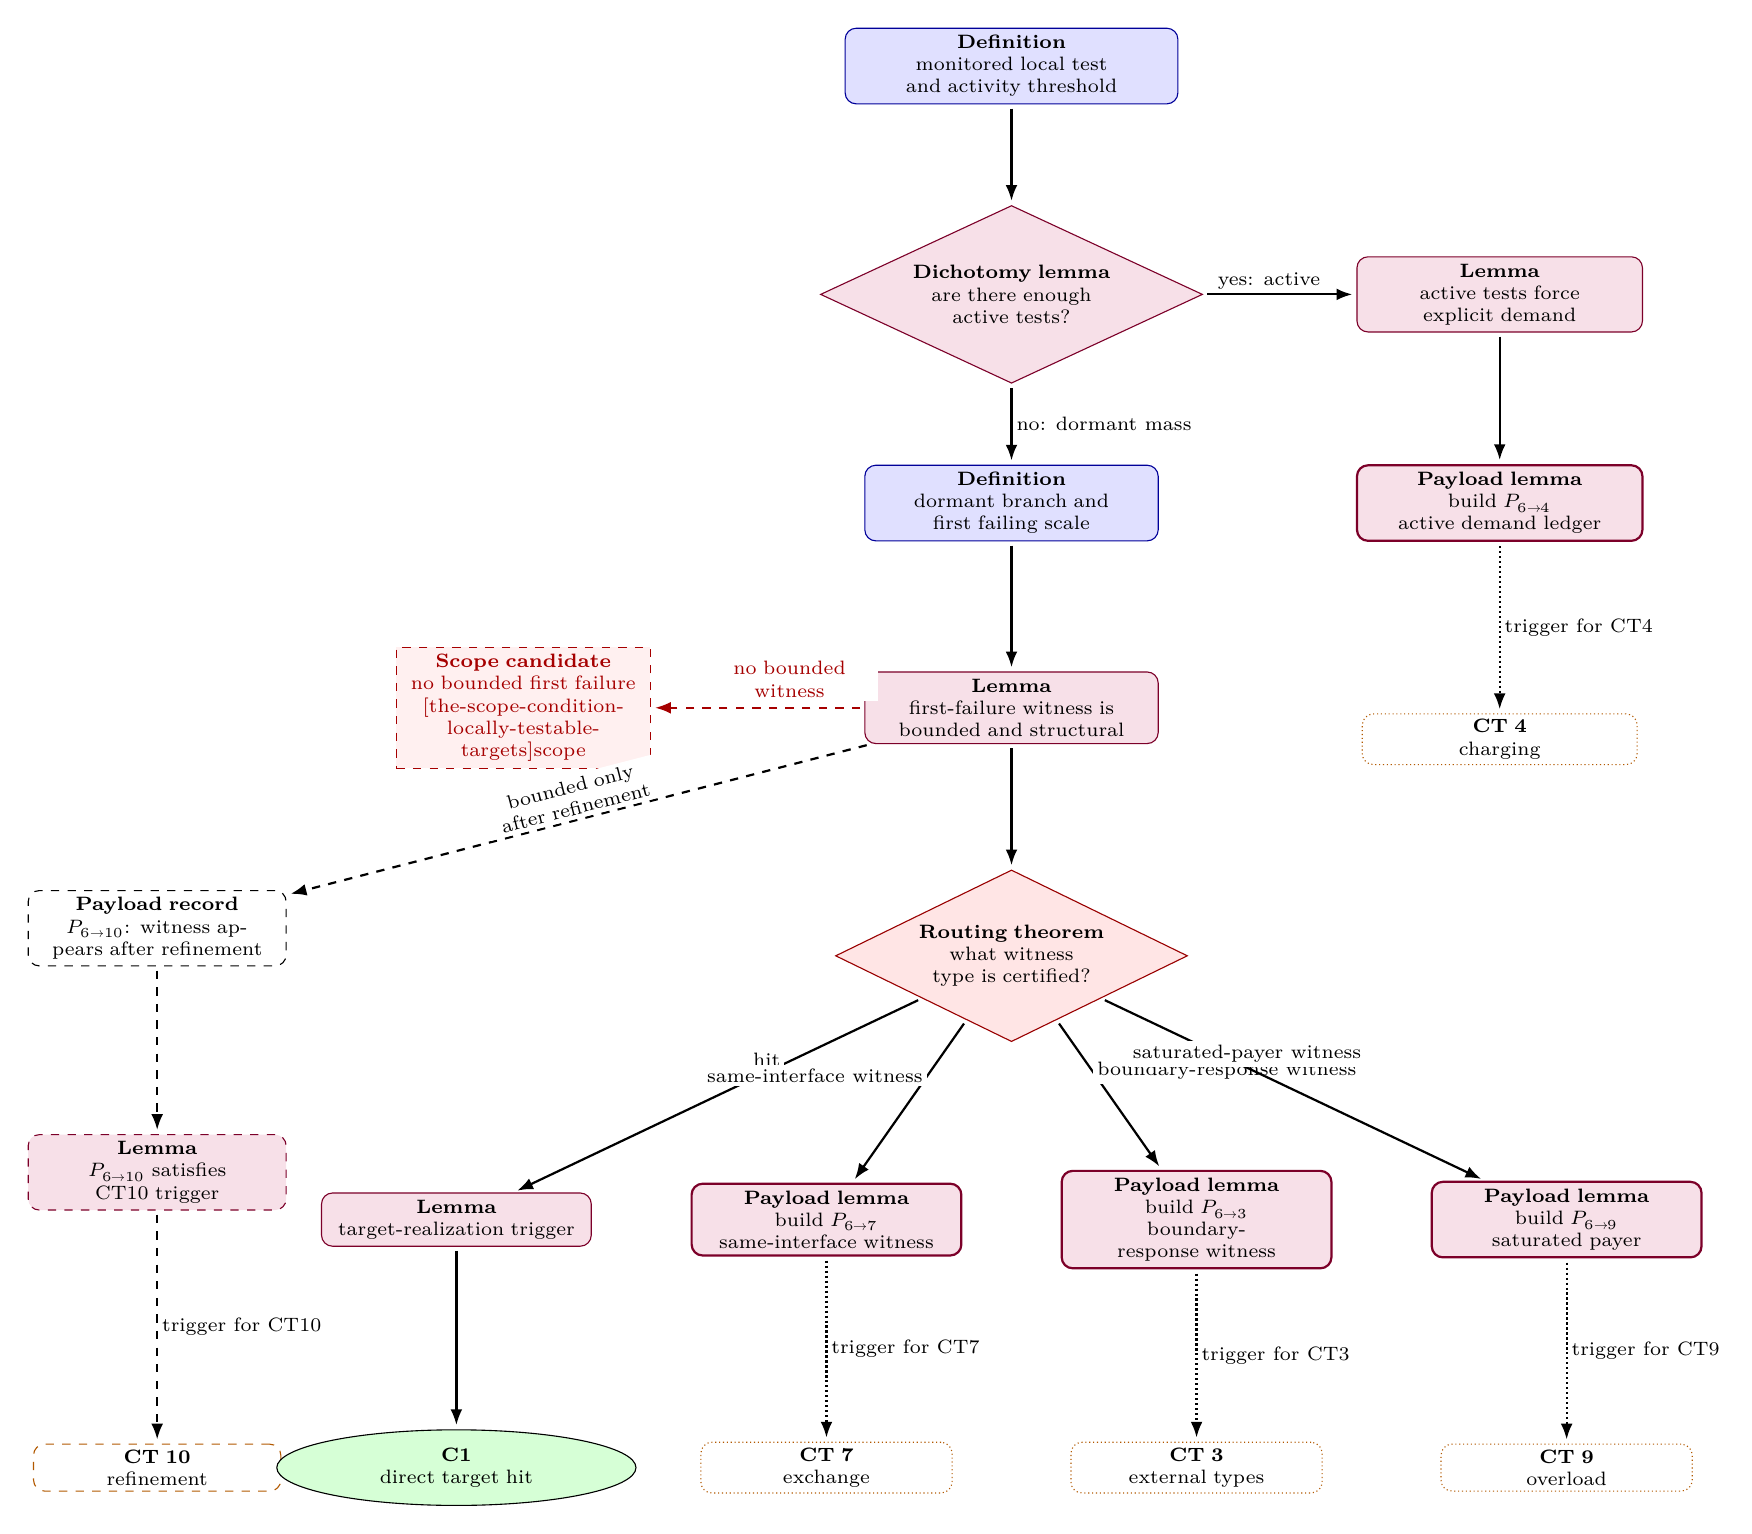
\begin{tikzpicture}[
every node/.style={font=\scriptsize}
]
\node[bcwide,bcdefinition] (input) at (0,0) {\textbf{Definition}\\monitored local test and activity threshold};
\node[bcdec,bclemma,text width=3.05cm,minimum width=3.85cm] (active) at (0,-2.90) {\textbf{Dichotomy lemma}\\are there enough active tests?};
\node[bcbox,bclemma,text width=3.45cm,minimum width=3.45cm] (hot) at (6.20,-2.90) {\textbf{Lemma}\\active tests force explicit demand};
\node[bcbox,bclemma,bcpayload,text width=3.45cm,minimum width=3.45cm] (hotout) at (6.20,-5.55) {\textbf{Payload lemma}\\build \(P_{6\to4}\)\\active demand ledger};
\node[bcroute,bcrouteneutral,bcoutputroute,text width=3.35cm,minimum width=3.35cm] (hotroute) at (6.20,-8.55) {\textbf{CT 4}\\charging};
\node[bcbox,bcdefinition,text width=3.55cm,minimum width=3.55cm] (cold) at (0,-5.55) {\textbf{Definition}\\dormant branch and first failing scale};
\node[bcbox,bclemma,text width=3.55cm,minimum width=3.55cm] (witness) at (0,-8.15) {\textbf{Lemma}\\first-failure witness is bounded and structural};
\node[bcscopefail,text width=3.05cm,minimum width=3.05cm] (scopebad) at (-6.20,-8.15) {\textbf{Scope candidate}\\no bounded first failure\\\scoperef};
\node[bcbox,bcdesign,text width=3.10cm,minimum width=3.10cm] (refineres) at (-10.85,-10.95) {\textbf{Payload record}\\\(P_{6\to10}\): witness appears after refinement};
\node[bcbox,bclemma,bcdesign,text width=3.10cm,minimum width=3.10cm] (refinelemma) at (-10.85,-14.05) {\textbf{Lemma}\\\(P_{6\to10}\) satisfies CT10 trigger};
\node[bcroute,bcrouteneutral,bcdesign,text width=3.00cm,minimum width=3.00cm] (refineroute) at (-10.85,-17.80) {\textbf{CT 10}\\refinement};
\node[bcroutechoice,bctheorem,text width=2.65cm,minimum width=3.30cm] (coldroute) at (0,-11.30) {\textbf{Routing theorem}\\what witness type is certified?};
\node[bcbox,bclemma,text width=3.25cm,minimum width=3.25cm] (hitlemma) at (-7.05,-14.65) {\textbf{Lemma}\\target-realization trigger};
\node[bcbox,bclemma,bcpayload,text width=3.25cm,minimum width=3.25cm] (exlemma) at (-2.35,-14.65) {\textbf{Payload lemma}\\build \(P_{6\to7}\)\\same-interface witness};
\node[bcbox,bclemma,bcpayload,text width=3.25cm,minimum width=3.25cm] (typelemma) at (2.35,-14.65) {\textbf{Payload lemma}\\build \(P_{6\to3}\)\\boundary-response witness};
\node[bcbox,bclemma,bcpayload,text width=3.25cm,minimum width=3.25cm] (chargellemma) at (7.05,-14.65) {\textbf{Payload lemma}\\build \(P_{6\to9}\)\\saturated payer};
\node[bcclosed,text width=3.05cm,minimum width=3.05cm] (hitout) at (-7.05,-17.80) {\textbf{C1}\\direct target hit};
\node[bcroute,bcrouteneutral,bcoutputroute,text width=3.05cm,minimum width=3.05cm] (exchangefig) at (-2.35,-17.80) {\textbf{CT 7}\\exchange};
\node[bcroute,bcrouteneutral,bcoutputroute,text width=3.05cm,minimum width=3.05cm] (typefig) at (2.35,-17.80) {\textbf{CT 3}\\external types};
\node[bcroute,bcrouteneutral,bcoutputroute,text width=3.05cm,minimum width=3.05cm] (chargefig) at (7.05,-17.80) {\textbf{CT 9}\\overload};
\draw[bcarr] (input)--(active);
\draw[bcarr] (active)--node[bclabel,pos=.43,above]{yes: active}(hot);
\draw[bcarr] (hot)--(hotout);
\draw[bchandoff] (hotout)--node[bclabel,right]{trigger for CT4}(hotroute);
\draw[bcarr] (active)--node[bclabel,right]{no: dormant mass}(cold);
\draw[bcarr] (cold)--(witness);
\draw[bcscopearr] (witness)--node[bclabel,above,pos=.35,yshift=2pt,text width=2.15cm,align=center]{no bounded witness}(scopebad);
\draw[bcrecoverarr] (witness)--node[bclabel,above,sloped,text width=2.20cm,align=center]{bounded only after refinement}(refineres);
\draw[bcrecoverarr] (refineres)--(refinelemma);
\draw[bcrecoverarr] (refinelemma)--node[bclabel,right]{trigger for CT10}(refineroute);
\draw[bcarr] (witness)--(coldroute);
\draw[bcarr] (coldroute)--node[bclabel,pos=.38,above]{hit}(hitlemma);
\draw[bcarr] (coldroute)--node[bclabel,pos=.34,left]{same-interface witness}(exlemma);
\draw[bcarr] (coldroute)--node[bclabel,pos=.34,right]{boundary-response witness}(typelemma);
\draw[bcarr] (coldroute)--node[bclabel,pos=.38,above]{saturated-payer witness}(chargellemma);
\draw[bcarr] (hitlemma)--(hitout);
\draw[bchandoff] (exlemma)--node[bclabel,right]{trigger for CT7}(exchangefig);
\draw[bchandoff] (typelemma)--node[bclabel,right]{trigger for CT3}(typefig);
\draw[bchandoff] (chargellemma)--node[bclabel,right]{trigger for CT9}(chargefig);
\end{tikzpicture}%
}
\caption[Closure-tactic 6: active/dormant dichotomy]{Closure-tactic 6 (active/dormant dichotomy).  The tactic is made rigorous by an activity-threshold definition, an active/dormant dichotomy lemma, an active-demand trigger for charging, a first-failure witness lemma, and a routing theorem whose cases certify direct target closure or construct typed payloads.  The active side builds \(P_{6\to4}\) for CT4; the dormant first-failure witness builds \(P_{6\to7}\), \(P_{6\to3}\), or \(P_{6\to9}\) according to whether the witness is same-interface, boundary-response, or saturated-payer data.  A bounded witness that appears only after refinement constructs the recovery residual \(P_{6\to10}\); absence of any bounded first-failure witness is a candidate scope obstruction referred to the global audit in \secref{the-scope-condition-locally-testable-targets}.  Line grammar (Fig.~\ref{fig:line-grammar-legend}): solid --- intended execution through the construction of the intended residual; dotted --- checks and the post-residual handoff to the consumer tactic; dashed --- design-failure recovery; red-dashed --- candidate scope obstruction referred to the global audit.}
\label{fig:ct6-active-dormant}
\end{figure}
\FloatBarrier

\subsection*{Active/dormant dichotomy in practice}

Many difficult proofs contain a dichotomy of the following kind:
the \textbf{active} or hot side is the branch on which the local test
fires and pays an \textbf{explicit charge}, meaning a contribution to a
demand count bounded from below; the \textbf{dormant} or cold side is
the branch on which that local test is inactive.

Dormancy is handled by the \textbf{first-failure principle}: when a
monitored property fails, the proof selects the minimal scale or index
at which failure first occurs; the bounded local data witnessing that
minimal failure is the \textbf{first-failure witness}. (The quantitative
form of the principle is given in \secref{structural-invariants-of-the-method}.) Schematically:

\[
\begin{gathered}
\text{dormant}
\;\Rightarrow\;
\text{first failure}
\;\Rightarrow\;
\text{bounded structural object}\\
\Rightarrow\;
\text{finite trichotomy}.
\end{gathered}
\]

In the abstract: (1) define activity relative to the actual branch
state; (2) if enough activity exists, count it; (3) if activity fails,
select the \emph{first} failure; (4) minimality of the first failure
supplies extra structure; (5) that structure is a direct target, a
defect, a compression, an overload, or a bounded exchange.

The quantitative form of the dichotomy deserves emphasis. When the
active branch fails \emph{linearly}, the entropy or counting cap that
the active tests would supply falls short by a definite margin. The
dormant family then has a \emph{linear lower bound} computable from that
margin. The dormant mass feeds the charging machinery of \secref{the-general-branch-closure-algorithm} and
\secref{the-charging-principle-in-general-form} with explicit constants. Thus the hot/cold split becomes a
quantitative case ledger: a finite table of density regimes, each row
carrying an exact numeric constraint and the name of the resource that
pays it.

The low-level diagram for CT6 is Fig.~\ref{fig:ct6-active-dormant};
it gives the activity dichotomy, first-failure witness, and the typed
routes from dormant mass to charging, types, exchange, or overload.



\subsection{CT7 --- Exchange trichotomy}\label{ct:7}\label{the-exchange-trichotomy}
\ctsignature{\(\begin{array}{@{}l@{}}
P_{\ast\to7}\to \ctcert{C1,C2,C3};\\
\ctint{P_{7\to3},P_{7\to12}};\\
\ctrec{P_{7\to10},P_{7\to16}}.
\end{array}\)}

You typically reach CT7 from CT6, CT8, CT9, CT10, CT11, or CT15 after a
bounded same-interface exchange has been exposed.  The question is
whether the exchange realizes the target, distinguishes the two
representatives, or is neutral.

\ctpar{Fires when}
The state contains an unclassified exchange pair
\((A,A',\iota,\delta)\) on a certified common interface.

\ctpar{You supply}
You supply a finite context generator \(\mathcal G(\iota)\), the
response evaluator restricted to \(\iota\)-completions, the size order,
and a same-interface table handle.

\ctpar{Execution}
First verify definition for \((A,A',\iota,\delta)\): the objects share the
interface, the exchange changes only declared support, and the response
evaluator is defined on \(\iota\)-completions.  Build
\(\mathcal G(\iota)\) from the recorded type components and test target
realization over it; a realizing context gives C1.  Next test separating
contexts.  A separator is packaged as \(P_{7\to3}\) when it is an
external-type defect, and as \(P_{7\to12}\) when it carries a routed
load measure.  On the separator-free branch, prove equivalence for generator
completeness before invoking neutral compression.  A smaller neutral
representative gives C2; the remaining neutral cases emit
\(P_{7\to10}\) or \(P_{7\to16}\) according to whether the missing datum
is a refinement label or a whole-object closed type.

\ctpar{Soundness obligations}
\begin{itemize}
\tightlist
\item \textbf{definition} is instantiated with the exchange pair \((A,A',\iota,\delta)\), the common interface, and the response evaluator on \(\iota\)-completions.
\item \textbf{equivalence} is instantiated with the completeness of the finite context generator \(\mathcal G(\iota)\) for all target-relevant compatible contexts.
\item \textbf{dichotomy} is instantiated with the realizing, distinguishing, and neutral alternatives for the bounded exchange.
\item \textbf{composition} is instantiated with the compression comparison for a smaller neutral representative.
\item \textbf{routing} is instantiated with \(P_{7\to3}\), \(P_{7\to12}\), \(P_{7\to10}\), and \(P_{7\to16}\) for external-type defects, peelable load, neutral labels, and whole-object data.
\item \textbf{trigger} is instantiated with the CT3, CT12, CT10, and CT16 triggers for those exchange outputs.
\end{itemize}

\ctpar{Routing}
Realization closes by C1.  A smaller neutral representative closes by
C2.  An already-routed defect closes by C3.  Remaining defects route to
CT3 or CT12; neutral residuals route to CT10 or CT16.

\ctpar{Limit}
CT7 is inapplicable when no finite context generator is available. The
execution error is declaring neutrality with equivalence unfilled; the audit
records CT7/equivalence.

\begin{figure}[p]
\centering
\vspace*{-2.80cm}
\resizebox{0.94\textwidth}{!}{%
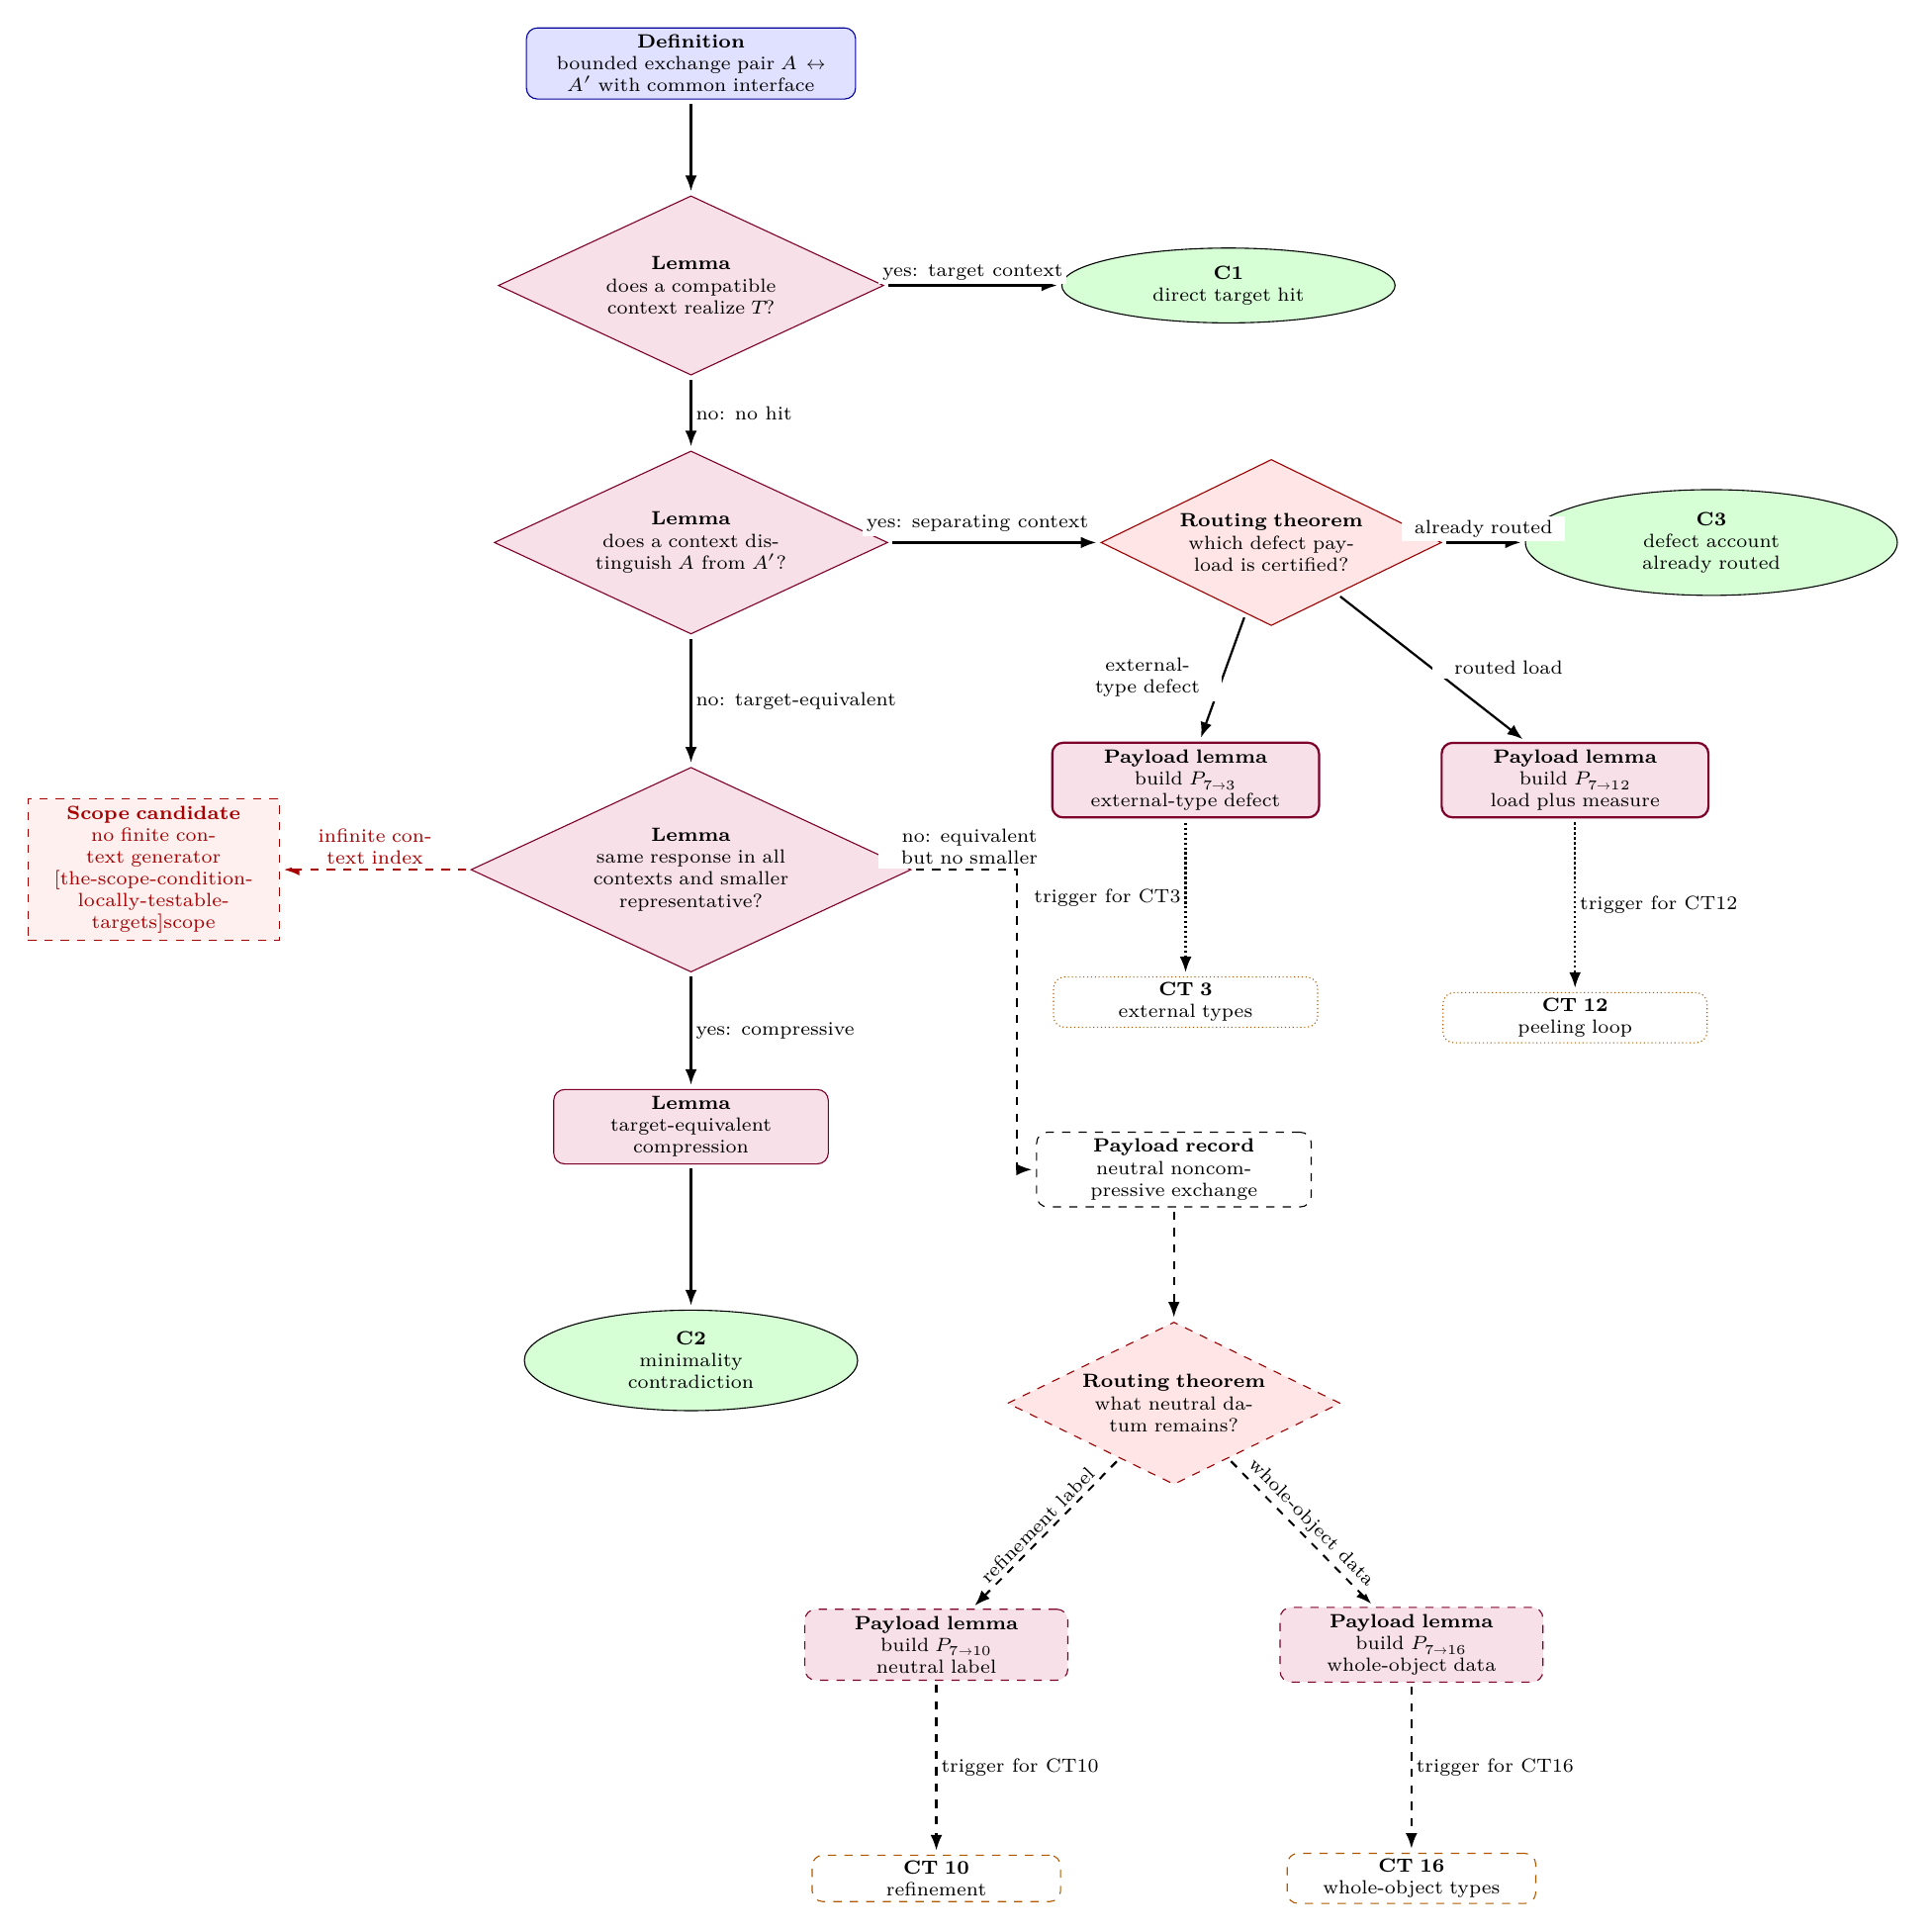
\begin{tikzpicture}[
every node/.style={font=\scriptsize}
]
\node[bcwide,bcdefinition] (input) at (0,0) {\textbf{Definition}\\bounded exchange pair \(A\leftrightarrow A'\) with common interface};
\node[bcdec,bclemma,text width=3.15cm,minimum width=3.95cm] (realize) at (0,-2.85) {\textbf{Lemma}\\does a compatible context realize \(T\)?};
\node[bcclosed] (hit) at (6.90,-2.85) {\textbf{C1}\\direct target hit};
\node[bcdec,bclemma,text width=3.15cm,minimum width=3.95cm] (distinguish) at (0,-6.15) {\textbf{Lemma}\\does a context distinguish \(A\) from \(A'\)?};
\node[bcroutechoice,bctheorem,text width=2.65cm,minimum width=3.25cm] (deflemma) at (7.45,-6.15) {\textbf{Routing theorem}\\which defect payload is certified?};
\node[bcclosed,text width=3.20cm,minimum width=3.20cm] (routedclose) at (13.10,-6.15) {\textbf{C3}\\defect account already routed};
\node[bcbox,bclemma,bcpayload,text width=3.25cm,minimum width=3.25cm] (extlemma) at (6.35,-9.20) {\textbf{Payload lemma}\\build \(P_{7\to3}\)\\external-type defect};
\node[bcroute,bcrouteneutral,bcoutputroute,text width=3.25cm,minimum width=3.25cm] (defect) at (6.35,-12.05) {\textbf{CT 3}\\external types};
\node[bcbox,bclemma,bcpayload,text width=3.25cm,minimum width=3.25cm] (peellemma) at (11.35,-9.20) {\textbf{Payload lemma}\\build \(P_{7\to12}\)\\load plus measure};
\node[bcroute,bcrouteneutral,bcoutputroute,text width=3.25cm,minimum width=3.25cm] (peeldefect) at (11.35,-12.25) {\textbf{CT 12}\\peeling loop};
\node[bcdec,bclemma,text width=3.15cm,minimum width=3.95cm] (neutral) at (0,-10.35) {\textbf{Lemma}\\same response in all contexts and smaller representative?};
\node[bcscopefail,text width=3.05cm,minimum width=3.05cm] (scopebad) at (-6.90,-10.35) {\textbf{Scope candidate}\\no finite context generator\\\scoperef};
\node[bcbox,bclemma,text width=3.35cm,minimum width=3.35cm] (complemma) at (0,-13.65) {\textbf{Lemma}\\target-equivalent compression};
\node[bcclosed] (compress) at (0,-16.65) {\textbf{C2}\\minimality contradiction};
\node[bcbox,bcdesign,text width=3.35cm,minimum width=3.35cm] (neutralres) at (6.20,-14.20) {\textbf{Payload record}\\neutral noncompressive exchange};
\node[bcroutechoice,bctheorem,bcdesign,text width=2.55cm,minimum width=3.15cm] (neutralroute) at (6.20,-17.20) {\textbf{Routing theorem}\\what neutral datum remains?};
\node[bcbox,bclemma,bcdesign,text width=3.20cm,minimum width=3.20cm] (reflemma) at (3.15,-20.30) {\textbf{Payload lemma}\\build \(P_{7\to10}\)\\neutral label};
\node[bcbox,bclemma,bcdesign,text width=3.20cm,minimum width=3.20cm] (exactlemma) at (9.25,-20.30) {\textbf{Payload lemma}\\build \(P_{7\to16}\)\\whole-object data};
\node[bcroute,bcrouteneutral,bcdesign,text width=3.05cm,minimum width=3.05cm] (refroute) at (3.15,-23.30) {\textbf{CT 10}\\refinement};
\node[bcroute,bcrouteneutral,bcdesign,text width=3.05cm,minimum width=3.05cm] (exactroute) at (9.25,-23.30) {\textbf{CT 16}\\whole-object types};
\draw[bcarr] (input)--(realize);
\draw[bcarr] (realize)--node[bclabel,above]{yes: target context}(hit);
\draw[bcarr] (realize)--node[bclabel,right]{no: no hit}(distinguish);
\draw[bcarr] (distinguish)--node[bclabel,above,pos=.42,yshift=2pt]{yes: separating context}(deflemma);
\draw[bcarr] (deflemma)--node[bclabel,above,text width=2.00cm,align=center]{already routed}(routedclose);
\draw[bcarr] (deflemma)--node[bclabel,left,text width=1.80cm,align=center]{external-type defect}(extlemma);
\draw[bchandoff] (extlemma)--node[bclabel,left]{trigger for CT3}(defect);
\draw[bcarr] (deflemma)--node[bclabel,right,text width=1.85cm,align=center]{routed load}(peellemma);
\draw[bchandoff] (peellemma)--node[bclabel,right]{trigger for CT12}(peeldefect);
\draw[bcarr] (distinguish)--node[bclabel,right]{no: target-equivalent}(neutral);
\draw[bcrecoverarr] (neutral.east) -- node[bclabel,above,text width=2.25cm,align=center,pos=.55]{no: equivalent but no smaller} ++(1.35,0) |- (neutralres.west);
\draw[bcscopearr] (neutral.west)--node[bclabel,above,pos=.50,text width=2.05cm,align=center]{infinite context index}(scopebad.east);
\draw[bcrecoverarr] (neutralres)--(neutralroute);
\draw[bcrecoverarr] (neutralroute)--node[bclabel,above,sloped]{refinement label}(reflemma);
\draw[bcrecoverarr] (neutralroute)--node[bclabel,above,sloped]{whole-object data}(exactlemma);
\draw[bcrecoverarr] (reflemma)--node[bclabel,right]{trigger for CT10}(refroute);
\draw[bcrecoverarr] (exactlemma)--node[bclabel,right]{trigger for CT16}(exactroute);
\draw[bcarr] (neutral)--node[bclabel,right]{yes: compressive}(complemma);
\draw[bcarr] (complemma)--(compress);
\end{tikzpicture}%
}
\caption[Closure-tactic 7: exchange trichotomy]{Closure-tactic 7 (exchange trichotomy).  A bounded exchange is certified by an exchange-pair definition, realizing and distinguishing lemmas, payload lemmas for the external-type or peelable-load route, and a neutral-compression lemma that closes by minimality when no distinguishing context exists.  The terminal exits are C1 for realization, C2 for neutral compression, and C3 when an existing defect account has already accepted responsibility.  A distinguishing defect constructs \(P_{7\to3}\) unless it carries the routed-load package \(P_{7\to12}\) required by the peeling loop; a certified neutral but noncompressive exchange constructs \(P_{7\to10}\) for refinement or \(P_{7\to16}\) for whole-object exact types.  Absence of a finite context generator is a candidate scope obstruction referred to the global audit in \secref{the-scope-condition-locally-testable-targets}.  Line grammar (Fig.~\ref{fig:line-grammar-legend}): solid --- intended execution through the construction of the intended residual; dotted --- checks and the post-residual handoff to the consumer tactic; dashed --- design-failure recovery; red-dashed --- candidate scope obstruction referred to the global audit.}
\label{fig:ct7-exchange-trichotomy}
\end{figure}
\FloatBarrier

\subsection*{Exchange trichotomy in practice}

Recall from \secref{the-branch-taxonomy} that a \textbf{local exchange} is a bounded local
operation that changes a target-relevant quantity by a bounded
increment, presented as two local representatives \(A\) and \(A'\) with
the same interface. This is the method's disciplined form of the
classical exchange and switching arguments. Every local exchange is
analyzed as follows.

\textbf{Realizing.} Some compatible context makes one representative
realize the target: $T(A\cup C)=1$. Close by target.

\textbf{Distinguishing.} Some context distinguishes the representatives:
$T(A\cup C)\ne T(A'\cup C)$. Route to a target defect.

\textbf{Neutral.} No context distinguishes the representatives:
$T(A\cup C)=T(A'\cup C)$ for all $C$. If one representative is
smaller, compress.

For a CT7 invocation with a certified finite context generator, the
declared outputs are

\[
\boxed{\ C1\mid C2\mid C3\mid
P_{7\to3}\mid P_{7\to12}\mid P_{7\to10}\mid P_{7\to16}\ }.
\]

The context-generator and equivalence completeness proofs are part of this
contract. Exchanges of increment zero enter a designated finite
same-interface table, where each entry is assigned one of the declared
outputs.

The low-level diagram for CT7 is Fig.~\ref{fig:ct7-exchange-trichotomy};
it is the formal checklist for realizing, distinguishing, neutral, and
whole-object exchange exits.



\subsection{CT8 --- Finite-state pumping}\label{ct:8}\label{the-finite-state-pumping-principle}
\ctsignature{\(P_{\ast\to8}\to \ctcert{C2,C5};\ \ctint{P_{8\to3},P_{8\to7}};\ \ctrec{P_{8\to10}}\).}

You reach CT8 when a branch produces a bounded-width sequence or chain.
The tactic converts length into repetition in a finite state alphabet and
then turns that repetition into compression or a separating witness.

\ctpar{Fires when}
The state contains a bounded sequence and a finite label or exact type
slot for each state.

\ctpar{You supply}
You supply the state alphabet, its explicit size bound, the equality
test, and the finite threshold.  The bound is recorded numerically; an
unnamed ``large enough'' threshold is not an input.

\ctpar{Execution}
Fix the alphabet, count its states, and apply the pigeonhole principle.
If two states have equal exact type, remove or replace the intervening
segment and close by minimality.  If their types differ, the first
distinguishing context is the payload.  Periodic means equal exact types.
A finite label space that is too coarse but exposes a bounded missing
datum constructs \(P_{8\to10}\); absence of any finite type space is the
scope boundary.

\ctpar{Soundness obligations}
\begin{itemize}
\tightlist
\item \textbf{definition} is instantiated with the bounded sequence \(S_0,\ldots,S_m\), the finite label or exact-type alphabet, and the equality test.
\item \textbf{dichotomy} is instantiated with the split between a repeated exact type and a short finite survivor list.
\item \textbf{equivalence} is instantiated with the claim that repeated types have equal response in all compatible contexts.
\item \textbf{composition} is instantiated with the finite threshold, the finite enumeration, or the repeated-type compression comparison.
\item \textbf{routing} is instantiated with \(P_{8\to3}\) for separating type data, \(P_{8\to7}\) for chain exchange data, and \(P_{8\to10}\) for a coarse finite label design.
\item \textbf{trigger} is instantiated with the CT3 trigger for separating types, the CT7 trigger for chain exchanges, and the CT10 trigger for finite label refinement.
\end{itemize}

\ctpar{Routing}
Equal repeated type closes by C2.  A short finite survivor list closes by
C5.  Separating type data routes to CT3; a chain exchange routes to CT7;
a finite missing label datum routes to CT10 as \(P_{8\to10}\).

\ctpar{Limit}
CT8 is inapplicable when no finite type space is available. A finite but
coarse label design is the typed recovery \(P_{8\to10}\).  The execution
error is informal periodicity; the audit records CT8/equivalence or CT8/dichotomy.

\begin{figure}[p]
\centering
\vspace*{-2.80cm}
\resizebox{!}{0.76\textheight}{%
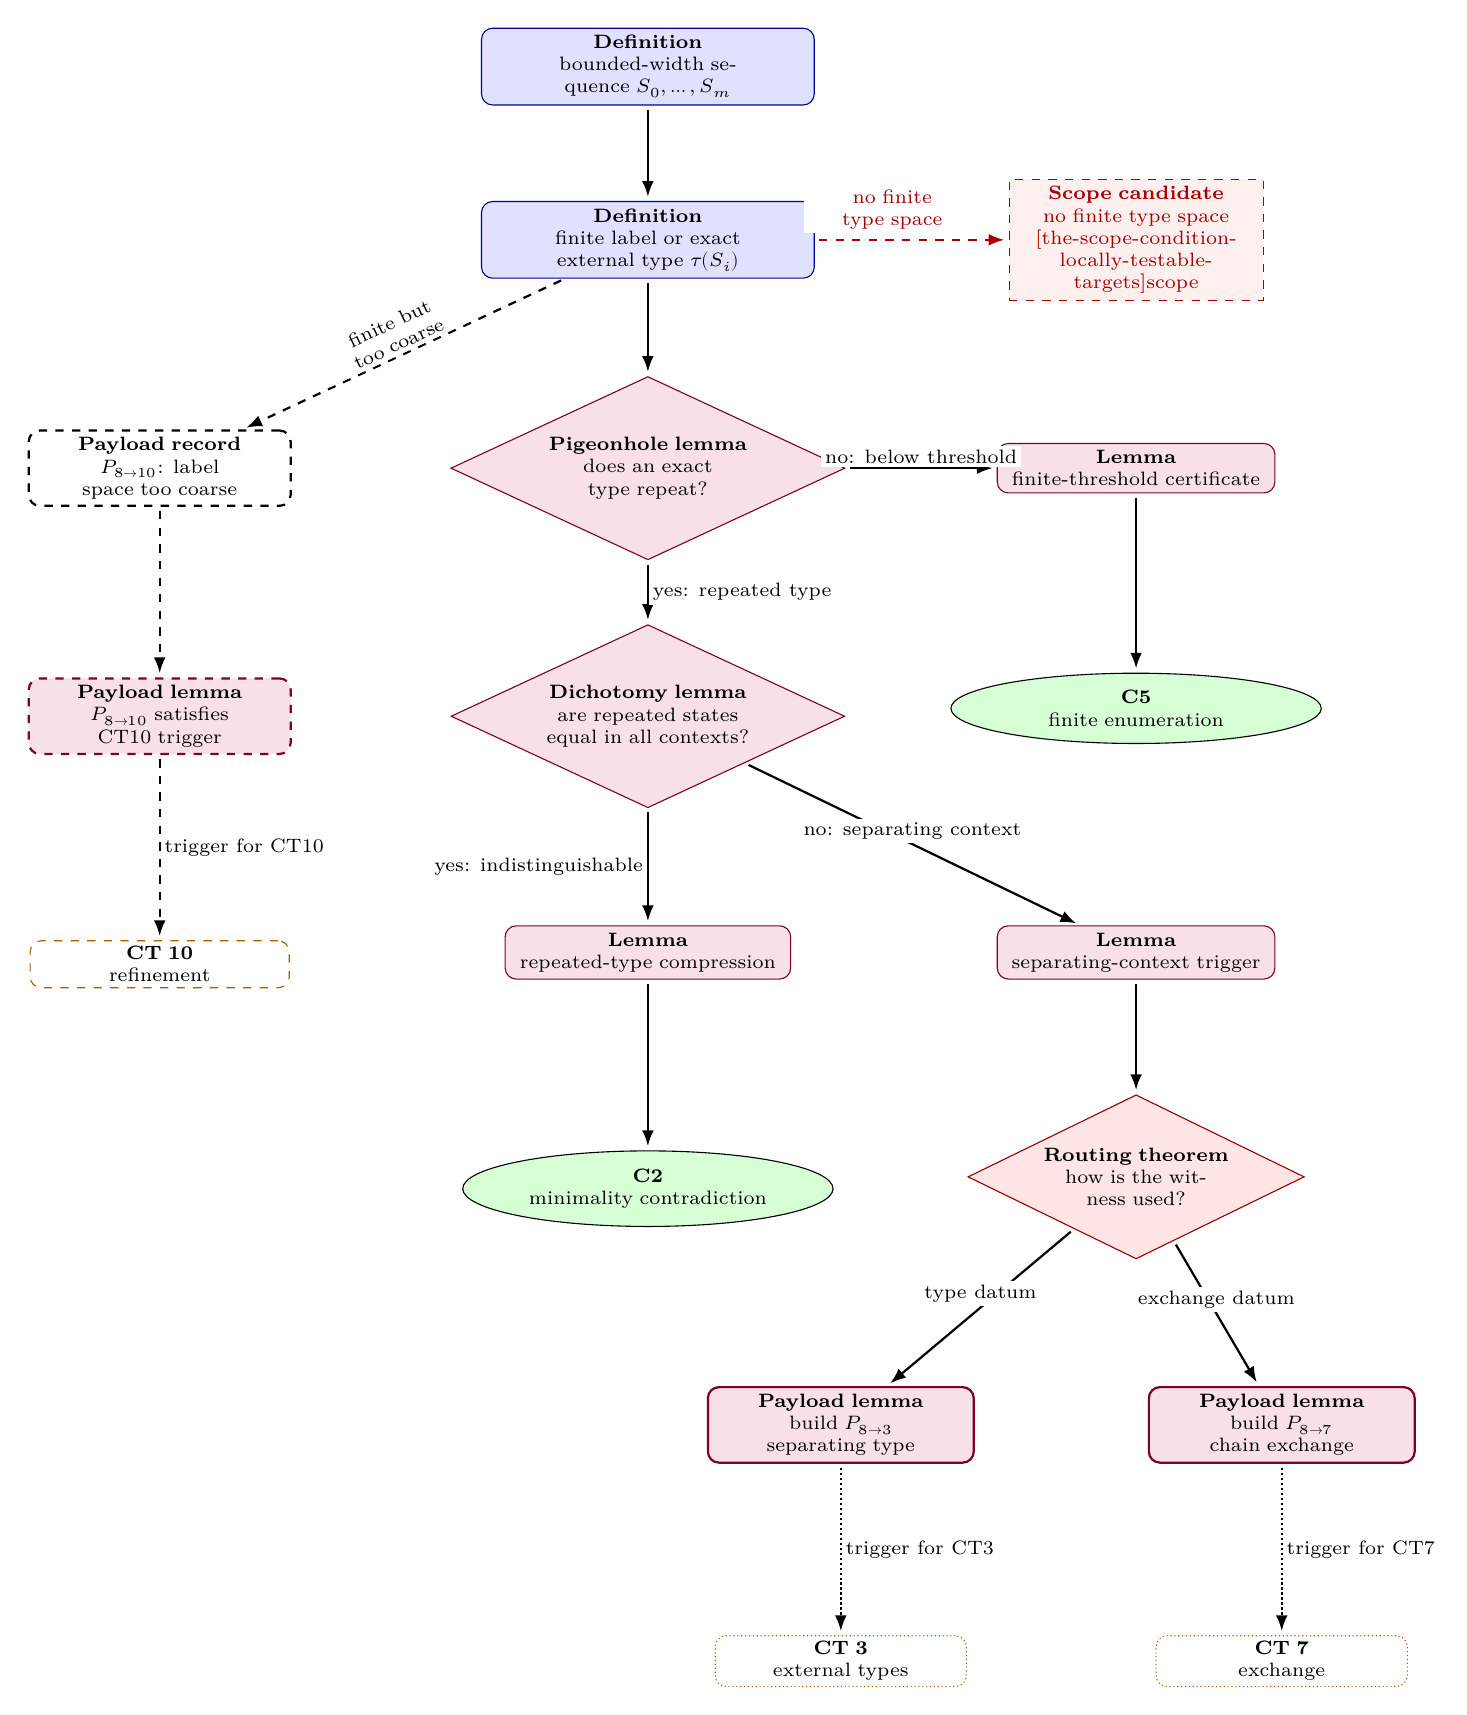
\begin{tikzpicture}[
every node/.style={font=\scriptsize}
]
\node[bcwide,bcdefinition] (input) at (0,0) {\textbf{Definition}\\bounded-width sequence \(S_0,\ldots,S_m\)};
\node[bcwide,bcdefinition] (types) at (0,-2.20) {\textbf{Definition}\\finite label or exact external type \(\tau(S_i)\)};
\node[bcscopefail,text width=3.05cm,minimum width=3.05cm] (scopebad) at (6.20,-2.20) {\textbf{Scope candidate}\\no finite type space\\\scoperef};
\node[bcbox,bcdesign,bcpayload,text width=3.15cm,minimum width=3.15cm] (labelres) at (-6.20,-5.10) {\textbf{Payload record}\\\(P_{8\to10}\): label space too coarse};
\node[bcbox,bclemma,bcdesign,bcpayload,text width=3.15cm,minimum width=3.15cm] (labeldesign) at (-6.20,-8.25) {\textbf{Payload lemma}\\\(P_{8\to10}\) satisfies CT10 trigger};
\node[bcroute,bcrouteneutral,bcdesign,text width=3.15cm,minimum width=3.15cm] (labelroute) at (-6.20,-11.40) {\textbf{CT 10}\\refinement};
\node[bcdec,bclemma,text width=3.10cm,minimum width=3.90cm] (repeat) at (0,-5.10) {\textbf{Pigeonhole lemma}\\does an exact type repeat?};
\node[bcbox,bclemma,text width=3.35cm,minimum width=3.35cm] (short) at (6.20,-5.10) {\textbf{Lemma}\\finite-threshold certificate};
\node[bcclosed,text width=3.15cm,minimum width=3.15cm] (shortroute) at (6.20,-8.15) {\textbf{C5}\\finite enumeration};
\node[bcdec,bclemma,text width=3.10cm,minimum width=3.90cm] (equal) at (0,-8.25) {\textbf{Dichotomy lemma}\\are repeated states equal in all contexts?};
\node[bcbox,bclemma,text width=3.35cm,minimum width=3.35cm] (defect) at (6.20,-11.25) {\textbf{Lemma}\\separating-context trigger};
\node[bcroutechoice,bctheorem,text width=2.55cm,minimum width=3.20cm] (defectroute) at (6.20,-14.10) {\textbf{Routing theorem}\\how is the witness used?};
\node[bcbox,bclemma,bcpayload,text width=3.20cm,minimum width=3.20cm] (typelemma) at (2.45,-17.25) {\textbf{Payload lemma}\\build \(P_{8\to3}\)\\separating type};
\node[bcbox,bclemma,bcpayload,text width=3.20cm,minimum width=3.20cm] (exlemma) at (8.05,-17.25) {\textbf{Payload lemma}\\build \(P_{8\to7}\)\\chain exchange};
\node[bcroute,bcrouteneutral,bcoutputroute,text width=3.05cm,minimum width=3.05cm] (typeroute) at (2.45,-20.25) {\textbf{CT 3}\\external types};
\node[bcroute,bcrouteneutral,bcoutputroute,text width=3.05cm,minimum width=3.05cm] (exroute) at (8.05,-20.25) {\textbf{CT 7}\\exchange};
\node[bcbox,bclemma,text width=3.45cm,minimum width=3.45cm] (complemma) at (0,-11.25) {\textbf{Lemma}\\repeated-type compression};
\node[bcclosed,text width=3.15cm,minimum width=3.15cm] (compress) at (0,-14.25) {\textbf{C2}\\minimality contradiction};
\draw[bcarr] (input)--(types);
\draw[bcscopearr] (types)--node[bclabel,above,pos=.40,yshift=2pt,text width=2.15cm,align=center]{no finite type space}(scopebad);
\draw[bcrecoverarr] (types)--node[bclabel,above,sloped,text width=1.95cm,align=center]{finite but too coarse}(labelres);
\draw[bcrecoverarr] (labelres)--(labeldesign);
\draw[bcrecoverarr] (labeldesign)--node[bclabel,right]{trigger for CT10}(labelroute);
\draw[bcarr] (types)--(repeat);
\draw[bcarr] (repeat)--node[bclabel,above]{no: below threshold}(short);
\draw[bcarr] (short)--(shortroute);
\draw[bcarr] (repeat)--node[bclabel,right]{yes: repeated type}(equal);
\draw[bcarr] (equal)--node[bclabel,above]{no: separating context}(defect);
\draw[bcarr] (defect)--(defectroute);
\draw[bcarr] (defectroute)--node[bclabel,above]{type datum}(typelemma);
\draw[bcarr] (defectroute)--node[bclabel,above]{exchange datum}(exlemma);
\draw[bchandoff] (typelemma)--node[bclabel,right]{trigger for CT3}(typeroute);
\draw[bchandoff] (exlemma)--node[bclabel,right]{trigger for CT7}(exroute);
\draw[bcarr] (equal)--node[bclabel,left]{yes: indistinguishable}(complemma);
\draw[bcarr] (complemma)--(compress);
\end{tikzpicture}%
}
\caption[Closure-tactic 8: finite-state pumping]{Closure-tactic 8 (finite-state pumping).  The tactic requires a bounded-sequence definition, a finite-type definition, a pigeonhole lemma, a finite-threshold certificate, a context-equivalence dichotomy lemma, a compression lemma for equal repeated types, and payload lemmas routing separating contexts to external types or exchange.  A separating context constructs \(P_{8\to3}\) for CT3 when the type datum is the output, and constructs \(P_{8\to7}\) for CT7 when the long chain exposes a bounded exchange.  A finite but coarse label space constructs the recovery payload \(P_{8\to10}\) for CT10; absence of any finite type space is a candidate scope obstruction referred to the global audit in \secref{the-scope-condition-locally-testable-targets}.  Line grammar (Fig.~\ref{fig:line-grammar-legend}): solid --- intended execution through the construction of the intended residual; dotted --- checks and the post-residual handoff to the consumer tactic; dashed --- design-failure recovery; red-dashed --- candidate scope obstruction referred to the global audit.}
\label{fig:ct8-finite-state-pumping}
\end{figure}
\FloatBarrier

\subsection*{Finite-state pumping in practice}

The name deliberately echoes the pumping lemma of automata theory: a
sequence with more elements than available states must repeat a state,
and the repetition is exploitable. As in the Myhill--Nerode and
Courcelle-style finite-state viewpoints, the relevant state is an
interface-complete response profile
\citep{myhill-1957-automata, nerode-1958-linear, courcelle-1990-mso-graphs, courcelle-engelfriet-2012-graph-structure}.

Whenever a branch produces a long chain, path, or sequence of
bounded-width states \(S_0, S_1, \ldots, S_m\), assign each state a
finite label or an exact external type. If \(m\) exceeds the number of
possible types, two types repeat.

If the repeated types are equal against all contexts,
\(\tau_i = \tau_j\), then the segment between them is removable or
replaceable, and minimality kills it. If the types differ, there is a
witness context, and that witness creates a target defect or a live
local test. A long chain must therefore hit the target, produce a
defect, or compress.

This is the abstract form of ``periodicity implies reducibility.'' In
this document, \emph{periodic} means equality of exact external types.
Congruence modulo a number and equality of informal labels are
insufficient.

The low-level diagram for CT8 is Fig.~\ref{fig:ct8-finite-state-pumping};
it connects the finite label space, pigeonhole step, equality test,
finite enumeration, and separating-context routes.



\subsection{CT9 --- Overload exhaustion}\label{ct:9}\label{the-charging-principle-in-general-form}
\ctsignature{\(P_{\ast\to9}\to \ctcert{C1};\ \ctint{P_{9\to4},P_{9\to7},P_{9\to8}};\ \ctrec{P_{9\to10}}\).}

You reach CT9 from CT4, CT6, CT13, or CT14 when a payer fibre threatens
the bounded-multiplicity claim.  The tactic proves bounded multiplicity
by exhausting the overcharged branch.

\ctpar{Fires when}
The state records a payer \(p\), its fibre \(F_p=\pi^{-1}(p)\), labels
on that fibre, and a certified capacity bound.

\ctpar{You supply}
You supply the finite label map, the fibre capacity, and the extraction
target.  The label choice is canonical, typically the largest recorded
class unless the charge-map definition specifies another tie-break.

\ctpar{Execution}
Assume the overloaded fibre and extract a homogeneous subfamily. The
instantiation must supply an extraction theorem whose exhaustive
alternatives map to CT9's declared leaves: a target hit, a same-interface
exchange, or a long chain. CT9 does not assert such a classification for
an arbitrary labelled family. Bounded multiplicity is proved by routing
every overload object, rather than asserted inside the original charge
lemma.

\ctpar{Soundness obligations}
\begin{itemize}
\tightlist
\item \textbf{definition} is instantiated with the payer \(p\), the fibre \(F_p=\pi^{-1}(p)\), the finite label map on the fibre, and the capacity bound.
\item \textbf{dichotomy} is instantiated with the bounded-fibre branch and the overloaded-fibre branch.
\item \textbf{composition} is instantiated with the pigeonhole or homogeneous-extraction comparison used to prove bounded multiplicity.
\item \textbf{routing} is instantiated with \(P_{9\to4}\), \(P_{9\to7}\), \(P_{9\to8}\), and \(P_{9\to10}\) for bounded multiplicity, homogeneous exchange, long-chain data, and finite-label recovery.
\item \textbf{trigger} is instantiated with the CT4, CT7, CT8, and CT10 triggers for those overload or recovery outputs.
\end{itemize}

\ctpar{Routing}
A target hit closes by C1.  If all fibres are bounded, CT9 returns
\(P_{9\to4}\) to CT4.  A homogeneous exchange routes to CT7, and a long
chain routes to CT8.  If the fibre labels are too coarse to support the
extraction, CT9 emits the recovery residual \(P_{9\to10}\).

\ctpar{Limit}
CT9 is inapplicable when no finite labelling is available. The execution error
is an unlabelled fibre or an undeclared tie-break; the audit records
CT9/definition.

\begin{figure}[p]
\centering
\vspace*{-2.80cm}
\resizebox{!}{0.76\textheight}{%
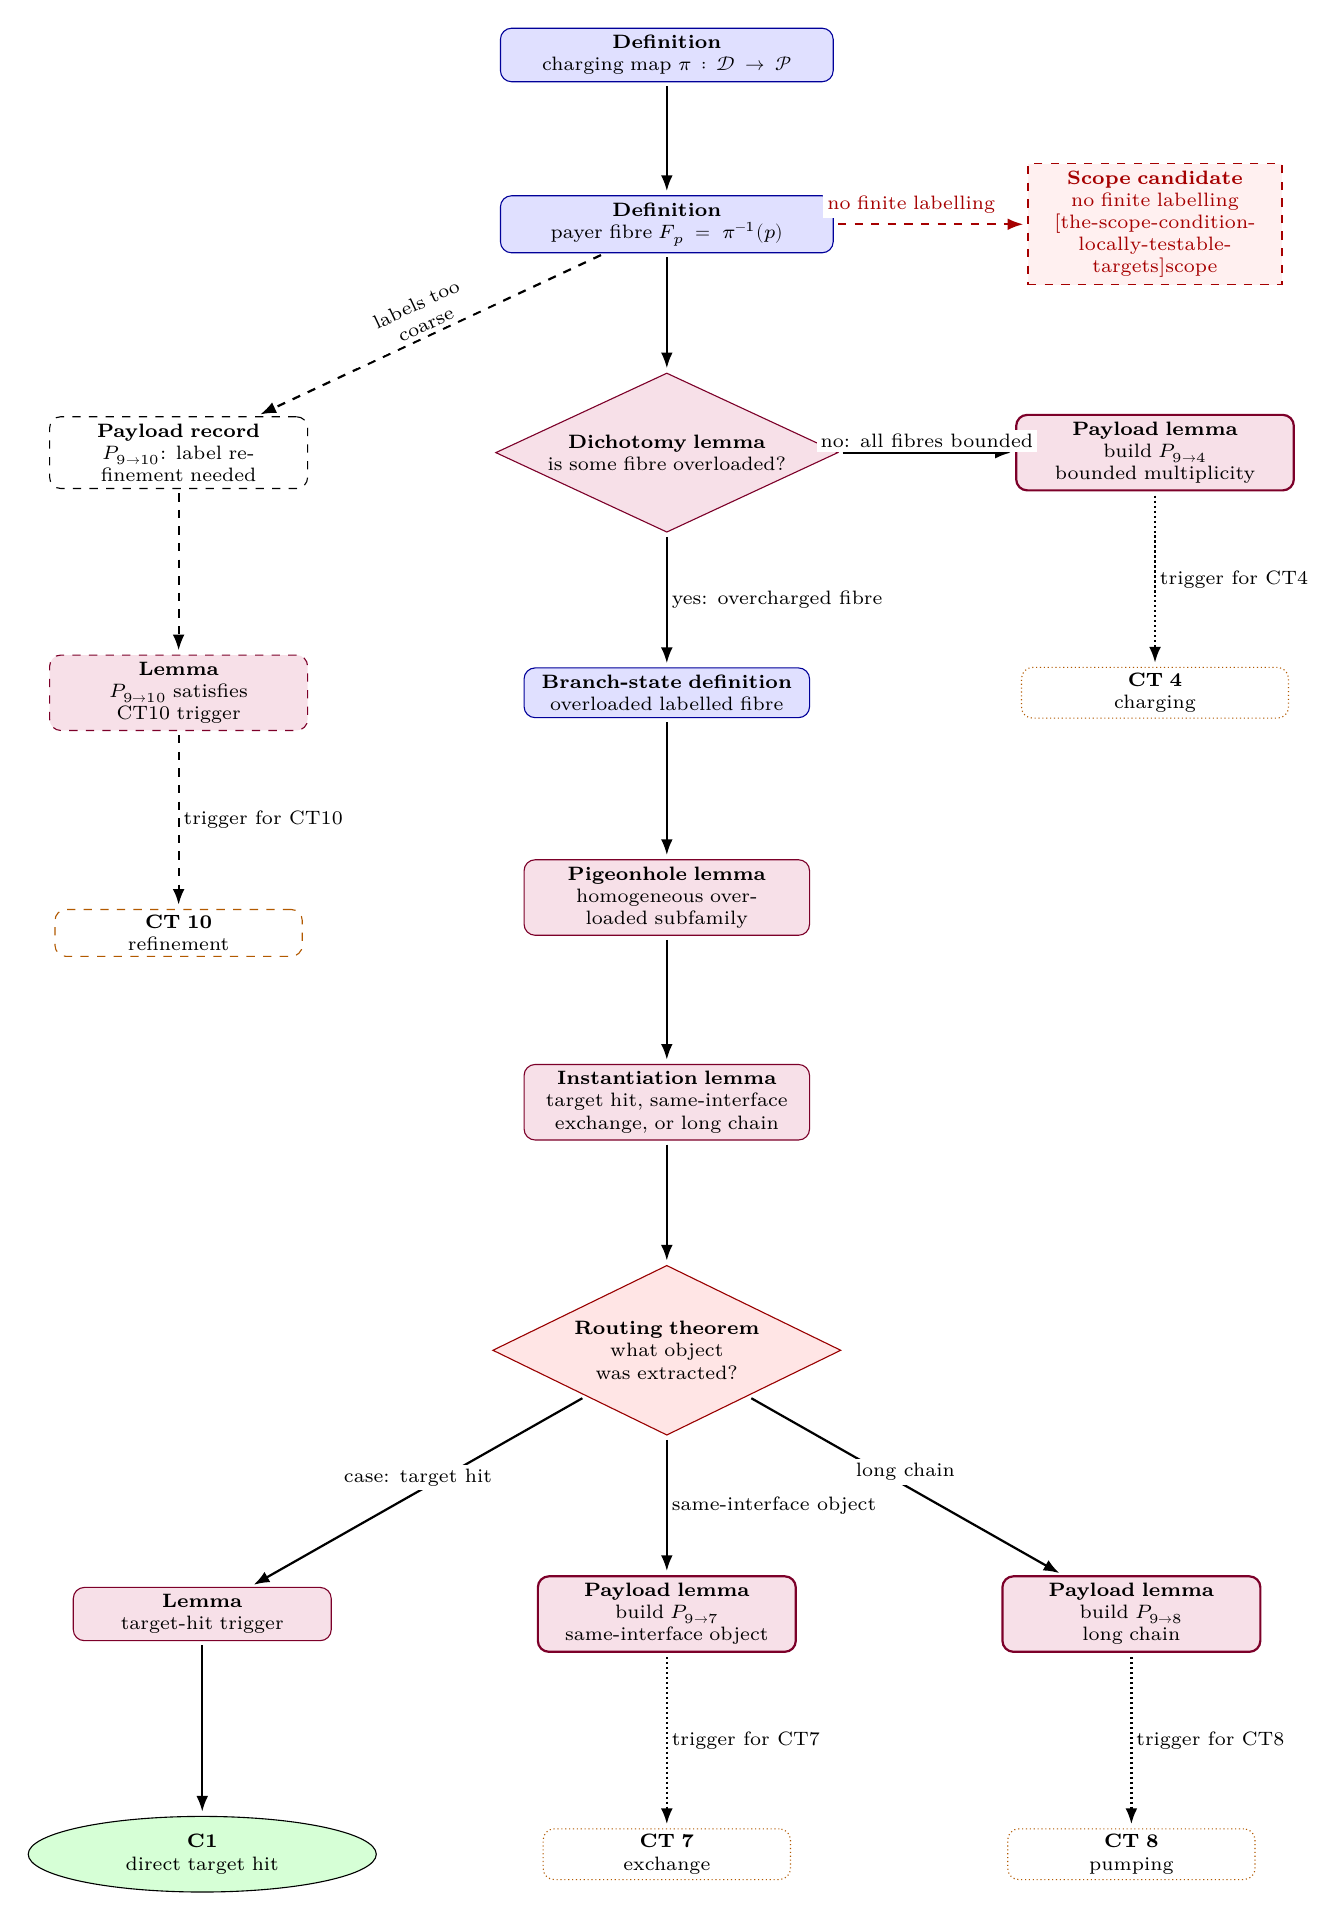
\begin{tikzpicture}[
every node/.style={font=\scriptsize}
]
\node[bcwide,bcdefinition] (input) at (0,0) {\textbf{Definition}\\charging map \(\pi:\mathcal D\to\mathcal P\)};
\node[bcwide,bcdefinition] (fiberdef) at (0,-2.15) {\textbf{Definition}\\payer fibre \(F_p=\pi^{-1}(p)\)};
\node[bcscopefail,text width=3.05cm,minimum width=3.05cm] (scopebad) at (6.20,-2.15) {\textbf{Scope candidate}\\no finite labelling\\\scoperef};
\node[bcbox,bcdesign,text width=3.10cm,minimum width=3.10cm] (labelres) at (-6.20,-5.05) {\textbf{Payload record}\\\(P_{9\to10}\): label refinement needed};
\node[bcbox,bclemma,bcdesign,text width=3.10cm,minimum width=3.10cm] (labellemma) at (-6.20,-8.10) {\textbf{Lemma}\\\(P_{9\to10}\) satisfies CT10 trigger};
\node[bcroute,bcrouteneutral,bcdesign,text width=3.00cm,minimum width=3.00cm] (labelroute) at (-6.20,-11.15) {\textbf{CT 10}\\refinement};
\node[bcdec,bclemma,text width=3.15cm,minimum width=4.00cm] (fiber) at (0,-5.05) {\textbf{Dichotomy lemma}\\is some fibre overloaded?};
\node[bcbox,bclemma,bcpayload,text width=3.35cm,minimum width=3.35cm] (bounded) at (6.20,-5.05) {\textbf{Payload lemma}\\build \(P_{9\to4}\)\\bounded multiplicity};
\node[bcroute,bcrouteneutral,bcoutputroute,text width=3.25cm,minimum width=3.25cm] (boundedroute) at (6.20,-8.10) {\textbf{CT 4}\\charging};
\node[bcbox,bcdefinition,text width=3.45cm,minimum width=3.45cm] (overload) at (0,-8.10) {\textbf{Branch-state definition}\\overloaded labelled fibre};
\node[bcbox,bclemma,text width=3.45cm,minimum width=3.45cm] (mono) at (0,-10.70) {\textbf{Pigeonhole lemma}\\homogeneous overloaded subfamily};
\node[bcbox,bclemma,text width=3.45cm,minimum width=3.45cm] (extract) at (0,-13.30) {\textbf{Instantiation lemma}\\target hit, same-interface exchange, or long chain};
\node[bcroutechoice,bctheorem,text width=2.70cm,minimum width=3.35cm] (route) at (0,-16.45) {\textbf{Routing theorem}\\what object was extracted?};
\node[bcbox,bclemma,text width=3.10cm,minimum width=3.10cm] (hitlemma) at (-5.90,-19.80) {\textbf{Lemma}\\target-hit trigger};
\node[bcbox,bclemma,bcpayload,text width=3.10cm,minimum width=3.10cm] (exchangelemma) at (0,-19.80) {\textbf{Payload lemma}\\build \(P_{9\to7}\)\\same-interface object};
\node[bcbox,bclemma,bcpayload,text width=3.10cm,minimum width=3.10cm] (pumplemma) at (5.90,-19.80) {\textbf{Payload lemma}\\build \(P_{9\to8}\)\\long chain};
\node[bcclosed,text width=2.95cm,minimum width=2.95cm] (hitout) at (-5.90,-22.85) {\textbf{C1}\\direct target hit};
\node[bcroute,bcrouteneutral,bcoutputroute,text width=3.00cm,minimum width=3.00cm] (exchangeout) at (0,-22.85) {\textbf{CT 7}\\exchange};
\node[bcroute,bcrouteneutral,bcoutputroute,text width=3.00cm,minimum width=3.00cm] (pumpout) at (5.90,-22.85) {\textbf{CT 8}\\pumping};
\draw[bcarr] (input)--(fiberdef);
\draw[bcscopearr] (fiberdef)--node[bclabel,above,pos=.40,yshift=2pt,text width=2.15cm,align=center]{no finite labelling}(scopebad);
\draw[bcrecoverarr] (fiberdef)--node[bclabel,above,sloped,text width=1.95cm,align=center]{labels too coarse}(labelres);
\draw[bcrecoverarr] (labelres)--(labellemma);
\draw[bcrecoverarr] (labellemma)--node[bclabel,right]{trigger for CT10}(labelroute);
\draw[bcarr] (fiberdef)--(fiber);
\draw[bcarr] (fiber)--node[bclabel,above]{no: all fibres bounded}(bounded);
\draw[bchandoff] (bounded)--node[bclabel,right]{trigger for CT4}(boundedroute);
\draw[bcarr] (fiber)--node[bclabel,right]{yes: overcharged fibre}(overload);
\draw[bcarr] (overload)--(mono);
\draw[bcarr] (mono)--(extract);
\draw[bcarr] (extract)--(route);
\draw[bcarr] (route)--node[bclabel,above]{case: target hit}(hitlemma);
\draw[bcarr] (route)--node[bclabel,right]{same-interface object}(exchangelemma);
\draw[bcarr] (route)--node[bclabel,above]{long chain}(pumplemma);
\draw[bcarr] (hitlemma)--(hitout);
\draw[bchandoff] (exchangelemma)--node[bclabel,right]{trigger for CT7}(exchangeout);
\draw[bchandoff] (pumplemma)--node[bclabel,right]{trigger for CT8}(pumpout);
\end{tikzpicture}%
}
\caption[Closure-tactic 9: overload exhaustion]{Closure-tactic 9 (overload exhaustion).  The tactic proves bounded multiplicity by defining payer fibres, splitting on overload, extracting a homogeneous overloaded subfamily, and applying a routing theorem whose payload lemmas close by target hit or route to exchange or pumping.  If all fibres are bounded, CT9 returns \(P_{9\to4}\) to CT4 as the bounded-multiplicity proof.  An overloaded homogeneous fibre constructs \(P_{9\to7}\) when it yields a same-interface object and \(P_{9\to8}\) when it yields a long chain.  The pigeonhole step is valid once the labelled fibre is finite; a failed finite-label design constructs the recovery residual \(P_{9\to10}\), while absence of any finite labelling is a candidate scope obstruction referred to the global audit in \secref{the-scope-condition-locally-testable-targets}.  Line grammar (Fig.~\ref{fig:line-grammar-legend}): solid --- intended execution through the construction of the intended residual; dotted --- checks and the post-residual handoff to the consumer tactic; dashed --- design-failure recovery; red-dashed --- candidate scope obstruction referred to the global audit.}
\label{fig:ct9-overload-exhaustion}
\end{figure}
\FloatBarrier

\subsection*{Overload exhaustion in practice}

Given demands \(\mathcal D\) and payers \(\mathcal P\), a charging
scheme is a map \(\pi:\mathcal D\to\mathcal P\), and the
bounded-multiplicity lemma asserts \(|\pi^{-1}(p)|\le C\) for every
\(p\), whence \(|\mathcal D|\le C|\mathcal P|\).

The crucial methodological point is that \textbf{bounded multiplicity is
proved by exhaustion of the overload branch.} If \(|\pi^{-1}(p)| > C\)
for some \(p\), then that fibre is overloaded; one extracts a
monochromatic subfamily, applies the instantiation-specific extraction
theorem, and routes its target-hit, same-interface-exchange, or long-chain
output. Equivalently,

\[
\text{overcount} \;\Rightarrow\;
\text{C1 or a typed residual for CT7, CT8, or CT10}.
\]

The low-level diagram for CT9 is Fig.~\ref{fig:ct9-overload-exhaustion};
it shows the payer-fibre dichotomy, homogeneous-overload extraction,
target-hit branch, and typed returns to CT4, CT7, and CT8.


\subsection{CT10 --- Default refinement}\label{ct:10}\label{the-default-refinement}
\ctsignature{\(P_{\ast\to10}\to \ctcert{C5};\ \ctint{P_{10\to3},P_{10\to7},P_{10\to15}};\ \ctrec{\ctnone}\).}

You reach CT10 when a residual survives the current invariants but
exposes a finite datum that was not yet named.  The tactic turns that
missing datum into the next label and reruns the classification on the
refined classes.

\ctpar{Fires when}
The state contains a residual class and a finite missing datum extracted
from a failed classification.

\ctpar{You supply}
You supply the candidate datum, the refined label alphabet, and the class
table.  These are synthesized by the invariant-and-label rule in
\secref{parameter-synthesis}.

\ctpar{Execution}
Define the promoted datum as a function of the recorded branch state and
form the refined finite alphabet \(\Lambda'\).  Partition the residual
class into the fibres of \(\Lambda'\), then run the local classification
theorem on each fibre.  A fibre exhausted by the finite table closes by
C5.  A bounded exchange inside a fibre constructs \(P_{10\to7}\); a
response or type datum constructs \(P_{10\to3}\); and a target-relative
rank datum constructs \(P_{10\to15}\).  When a fibre remains
unclassified, the classification theorem must name the next branch-state
datum before CT10 iterates.  The promoted datum is then recorded as the
next invariant, together with its finite alphabet and trigger payload.

\ctpar{Soundness obligations}
\begin{itemize}
\tightlist
\item \textbf{definition} is instantiated with the residual class, the promoted finite datum, the refined alphabet \(\Lambda'\), and the class table.
\item \textbf{dichotomy} is instantiated with the refined label-class alternatives produced by \(\Lambda'\).
\item \textbf{composition} is instantiated with the finite class-exhaustion check inside each refined label class.
\item \textbf{routing} is instantiated with \(P_{10\to3}\), \(P_{10\to7}\), and \(P_{10\to15}\) for promoted response data, class exchanges, and rank data.
\item \textbf{trigger} is instantiated with the CT3, CT7, and CT15 triggers for the promoted payloads.
\end{itemize}

\ctpar{Routing}
Finite class exhaustion closes by C5.  Promoted response data routes to
CT3, class exchanges route to CT7, and rank data routes to CT15.

\ctpar{Limit}
CT10 is inapplicable when every adequate refinement alphabet is infinite. The execution
error is failing to extract the promoted datum from the classification;
the audit records CT10/definition or CT10/routing.

\begin{figure}[p]
\centering
\vspace*{-2.80cm}
\resizebox{!}{0.76\textheight}{%
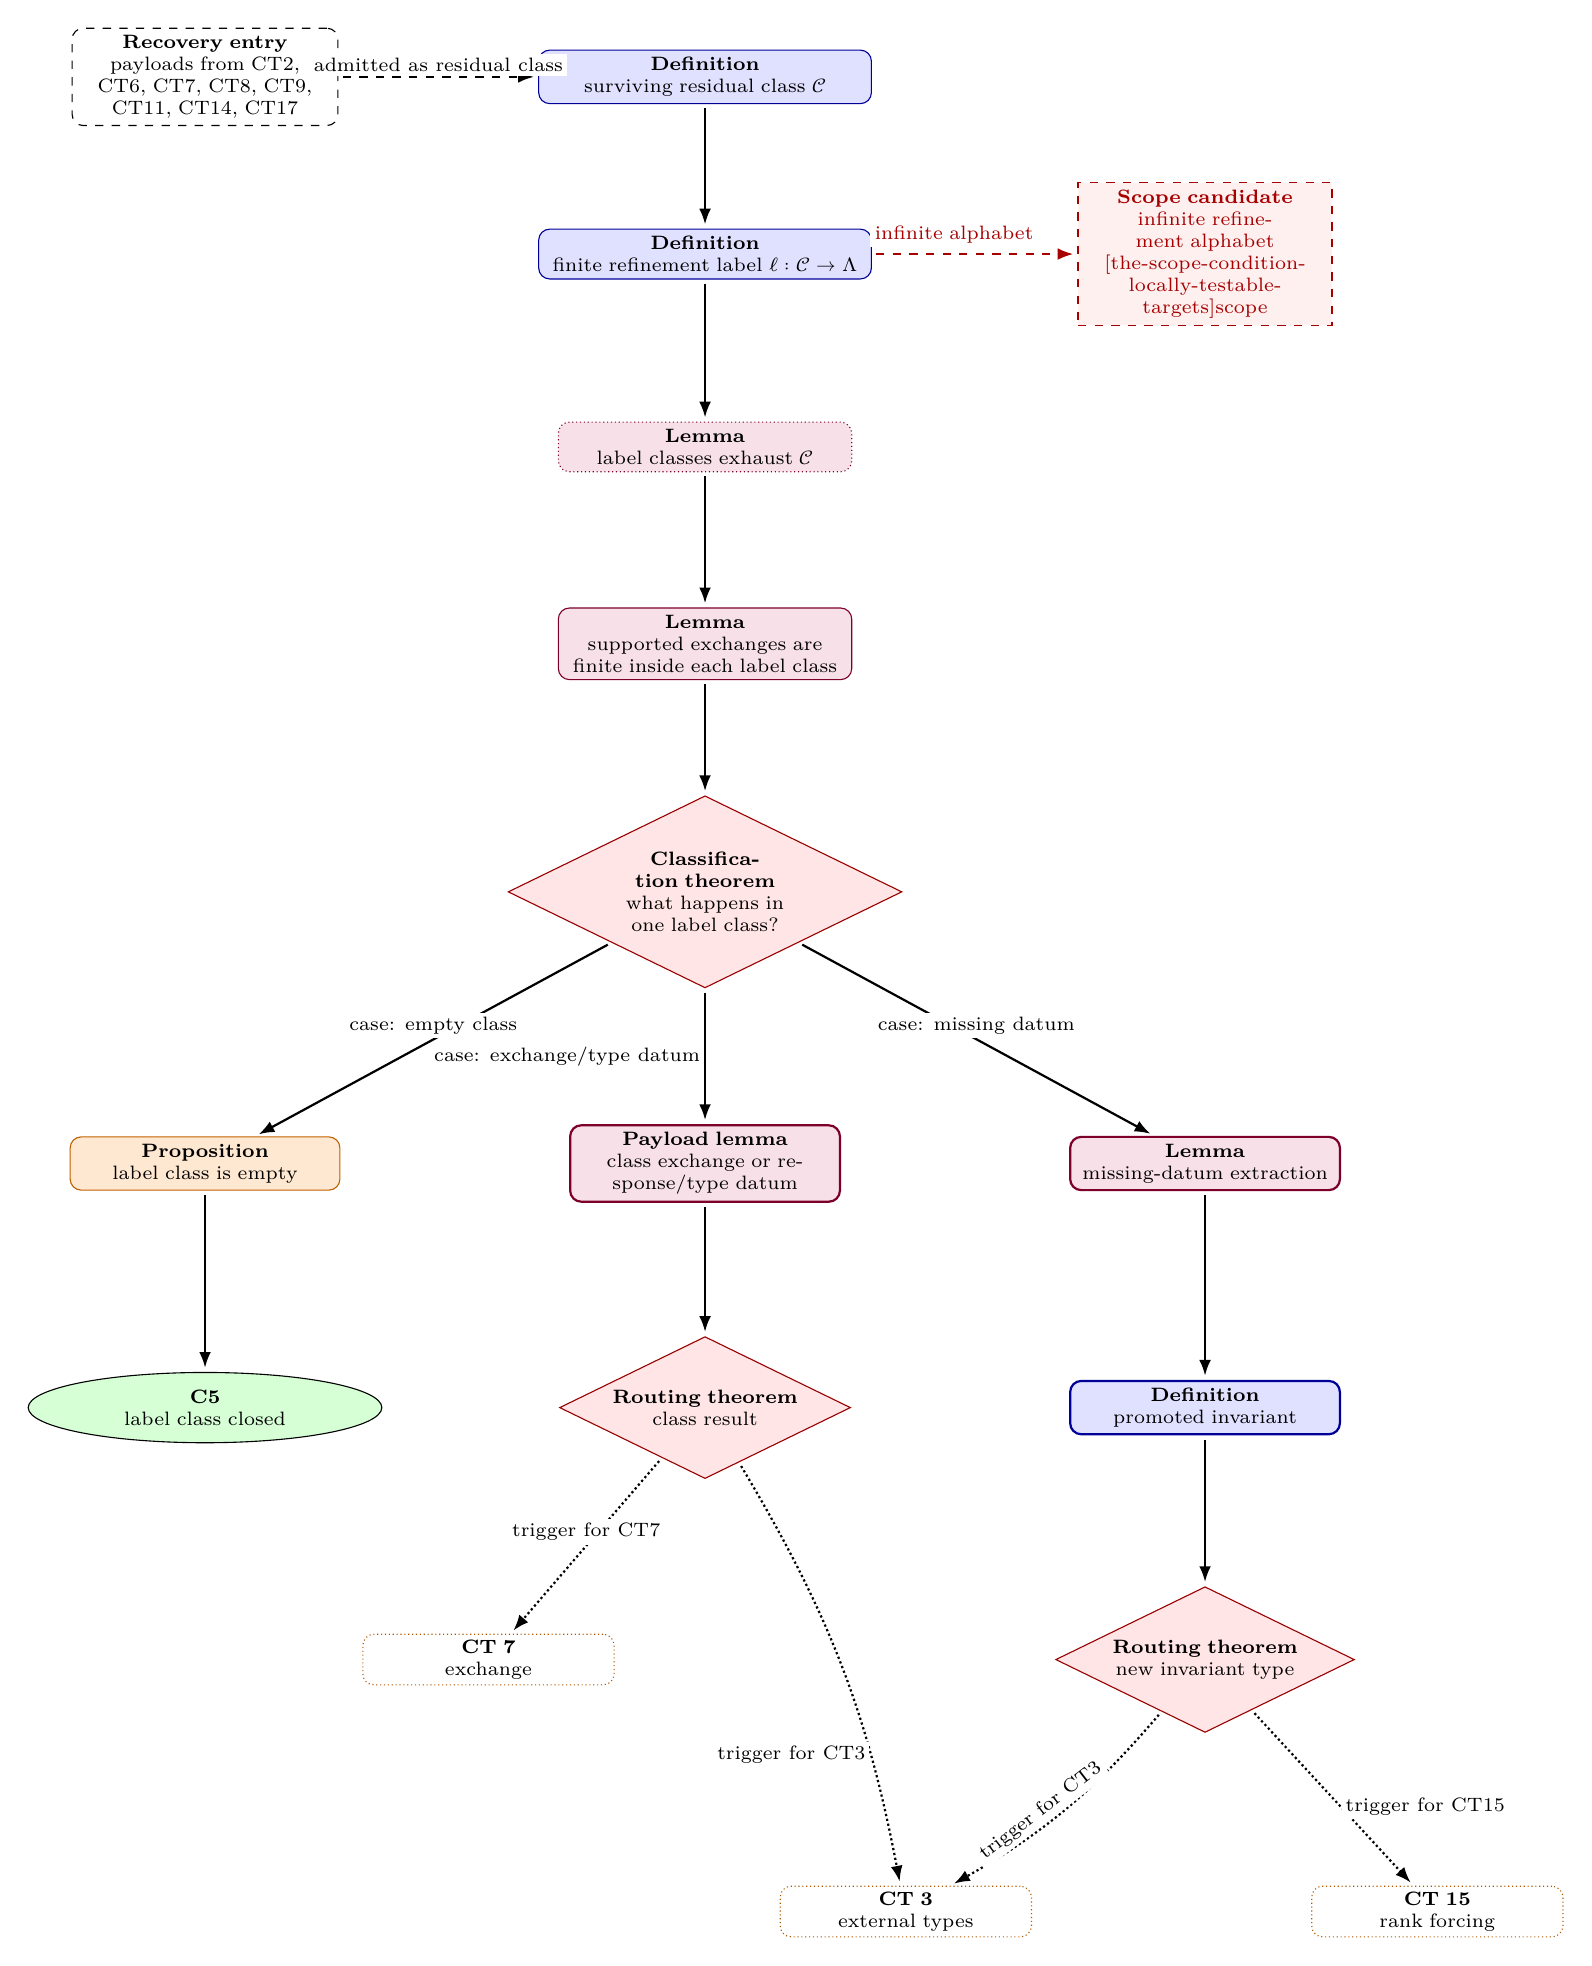
\begin{tikzpicture}[
every node/.style={font=\scriptsize}
]
\node[bcwide,bcdefinition] (input) at (0,0) {\textbf{Definition}\\surviving residual class \(\mathcal C\)};
\node[bcbox,bcdesign,text width=3.20cm,minimum width=3.20cm] (recoverentry) at (-6.35,0) {\textbf{Recovery entry}\\payloads from CT2, CT6, CT7, CT8, CT9, CT11, CT14, CT17};
\node[bcwide,bcdefinition] (label) at (0,-2.25) {\textbf{Definition}\\finite refinement label \(\ell:\mathcal C\to\Lambda\)};
\node[bcscopefail,text width=3.05cm,minimum width=3.05cm] (scopebad) at (6.35,-2.25) {\textbf{Scope candidate}\\infinite refinement alphabet\\\scoperef};
\node[bcbox,bclemma,bccheck,text width=3.55cm,minimum width=3.55cm] (exhaust) at (0,-4.70) {\textbf{Lemma}\\label classes exhaust \(\mathcal C\)};
\node[bcbox,bclemma,text width=3.55cm,minimum width=3.55cm] (exchange) at (0,-7.20) {\textbf{Lemma}\\supported exchanges are finite inside each label class};
\node[bcroutechoice,bctheorem,text width=2.70cm,minimum width=3.40cm] (outcome) at (0,-10.35) {\textbf{Classification theorem}\\what happens in one label class?};
\node[bcbox,bcproposition,text width=3.25cm,minimum width=3.25cm] (closeprop) at (-6.35,-13.80) {\textbf{Proposition}\\label class is empty};
\node[bcclosed,text width=3.00cm,minimum width=3.00cm] (classclose) at (-6.35,-16.90) {\textbf{C5}\\label class closed};
\node[bcbox,bclemma,bcpayload,text width=3.25cm,minimum width=3.25cm] (routelemma) at (0,-13.80) {\textbf{Payload lemma}\\class exchange or response/type datum};
\node[bcroutechoice,bctheorem,text width=2.55cm,minimum width=3.20cm] (closeroute) at (0,-16.90) {\textbf{Routing theorem}\\class result};
\node[bcroute,bcrouteneutral,bcoutputroute,text width=3.05cm,minimum width=3.05cm] (exchangefig) at (-2.75,-20.10) {\textbf{CT 7}\\exchange};
\node[bcroute,bcrouteneutral,bcoutputroute,text width=3.05cm,minimum width=3.05cm] (typefig) at (2.55,-23.30) {\textbf{CT 3}\\external types};
\node[bcbox,bclemma,bcpayload,text width=3.25cm,minimum width=3.25cm] (promote) at (6.35,-13.80) {\textbf{Lemma}\\missing-datum extraction};
\node[bcbox,bcdefinition,bcpayload,text width=3.25cm,minimum width=3.25cm] (next) at (6.35,-16.90) {\textbf{Definition}\\promoted invariant};
\node[bcroutechoice,bctheorem,text width=2.55cm,minimum width=3.20cm] (nextfig) at (6.35,-20.10) {\textbf{Routing theorem}\\new invariant type};
\node[bcroute,bcrouteneutral,bcoutputroute,text width=3.05cm,minimum width=3.05cm] (rankgen) at (9.30,-23.30) {\textbf{CT 15}\\rank forcing};
\draw[bcrecoverarr] (recoverentry)--node[bclabel,above]{admitted as residual class}(input);
\draw[bcarr] (input)--(label);
\draw[bcscopearr] (label)--node[bclabel,above,pos=.40,yshift=2pt,text width=2.05cm,align=center]{infinite alphabet}(scopebad);
\draw[bcarr] (label)--(exhaust);
\draw[bcarr] (exhaust)--(exchange);
\draw[bcarr] (exchange)--(outcome);
\draw[bcarr] (outcome)--node[bclabel,above]{case: empty class}(closeprop);
\draw[bcarr] (closeprop)--(classclose);
\draw[bcarr] (outcome)--node[bclabel,left]{case: exchange/type datum}(routelemma);
\draw[bcarr] (routelemma)--(closeroute);
\draw[bchandoff] (closeroute)--node[bclabel,above]{trigger for CT7}(exchangefig);
\draw[bchandoff] (closeroute) to[bend left=10] node[bclabel,left,pos=.72]{trigger for CT3}(typefig);
\draw[bcarr] (outcome)--node[bclabel,above]{case: missing datum}(promote);
\draw[bcarr] (promote)--(next);
\draw[bcarr] (next)--(nextfig);
\draw[bchandoff] (nextfig) to[bend left=10] node[bclabel,above,sloped,pos=.58]{trigger for CT3}(typefig);
\draw[bchandoff] (nextfig)--node[bclabel,right,pos=.55]{trigger for CT15}(rankgen);
\end{tikzpicture}%
}
\caption[Closure-tactic 10: default refinement]{Closure-tactic 10 (default refinement).  The tactic is certified by a residual-class definition, a finite-label definition, a label-exhaustion lemma, a finite exchange-support lemma, a classification theorem for each label class, payload lemmas for exchange or response-type routes, and a missing-datum extraction lemma that promotes the next invariant.  A bounded class exchange constructs \(P_{10\to7}\); a response or type datum constructs \(P_{10\to3}\); and a rank datum constructs \(P_{10\to15}\).  The extracted datum is the promoted residual; an infinite refinement alphabet is a candidate scope obstruction referred to the global audit in \secref{the-scope-condition-locally-testable-targets}.  Line grammar (Fig.~\ref{fig:line-grammar-legend}): solid --- intended execution through the construction of the intended residual; dotted --- checks and the post-residual handoff to the consumer tactic; dashed --- design-failure recovery; red-dashed --- candidate scope obstruction referred to the global audit.}
\label{fig:ct10-default-refinement}
\end{figure}
\FloatBarrier

\subsection*{Default refinement in practice}

Given CT10's admitted residual class and finite label data, the
\textbf{default refinement} stratifies the residual by that label. Inside
each label class, run the exchange trichotomy (\secref{the-exchange-trichotomy}) on the bounded
exchanges the class supports. One of three things happens: the class
closes; an exchange or response-type datum appears and routes; or the analysis
reveals precisely which datum the label is missing. That datum, promoted
to the label or to the type, is the next invariant.

The low-level diagram for CT10 is Fig.~\ref{fig:ct10-default-refinement};
it displays the finite label exhaustion, class-level classification,
and the payloads routed to CT3, CT7, and CT15.



\subsection{CT11 --- Localization}\label{ct:11}\label{additivity-and-the-localization-lemma}
\ctsignature{\(P_{5\to11}\to \ctcert{\ctnone};\ \ctint{P_{11\to1},P_{11\to7},P_{11\to14}};\ \ctrec{P_{11\to10}}\).}

You reach CT11 when a global additive deficit has been recorded but the
proof needs a bounded local piece.  The tactic is an averaging step with
an admissibility check attached.

\ctpar{Fires when}
The branch state contains an additive budget deficit and an admissible
decomposition of the ambient object into connected pieces.

\ctpar{You supply}
You supply the budget, the admissibility class, and the decomposition
lemma.  \secref{part-iii-the-strategy-manual} supplies the budget normal form and the closure of the
class under the local moves that will be used later.

\ctpar{Execution}
Decompose the object into connected admissible pieces and apply the
first-moment argument: if the total deficit is negative, one admissible
piece has negative local budget.  The admissibility-closure lemma is
stated before localization is invoked; otherwise the localized piece may
fall outside the tactic library.

\ctpar{Soundness obligations}
\begin{itemize}
\tightlist
\item \textbf{definition} is instantiated with the additive budget, the admissible decomposition, the admissibility class, and the localized piece data.
\item \textbf{composition} is instantiated with the summation and averaging comparison that produces a connected local piece with negative budget.
\item \textbf{routing} is instantiated with \(P_{11\to1}\), \(P_{11\to7}\), \(P_{11\to10}\), and \(P_{11\to14}\) for target-test data, localized exchange data, admissibility gaps, and carried mass.
\item \textbf{trigger} is instantiated with the CT1, CT7, CT10, and CT14 triggers for those localized outputs.
\end{itemize}

\ctpar{Routing}
The local piece may carry target-test data for CT1, exchange data for
CT7, a finite admissibility gap for CT10, or aggregate carried mass for
CT14.  CT11 is route-only; it has no certificate sink of its own.

\ctpar{Limit}
CT11 is inapplicable when no additive bounded local type is available. The
execution error is invoking localization before admissibility closure is
proved; the audit records CT11/definition.

\begin{figure}[p]
\centering
\vspace*{-2.80cm}
\resizebox{!}{0.68\textheight}{%
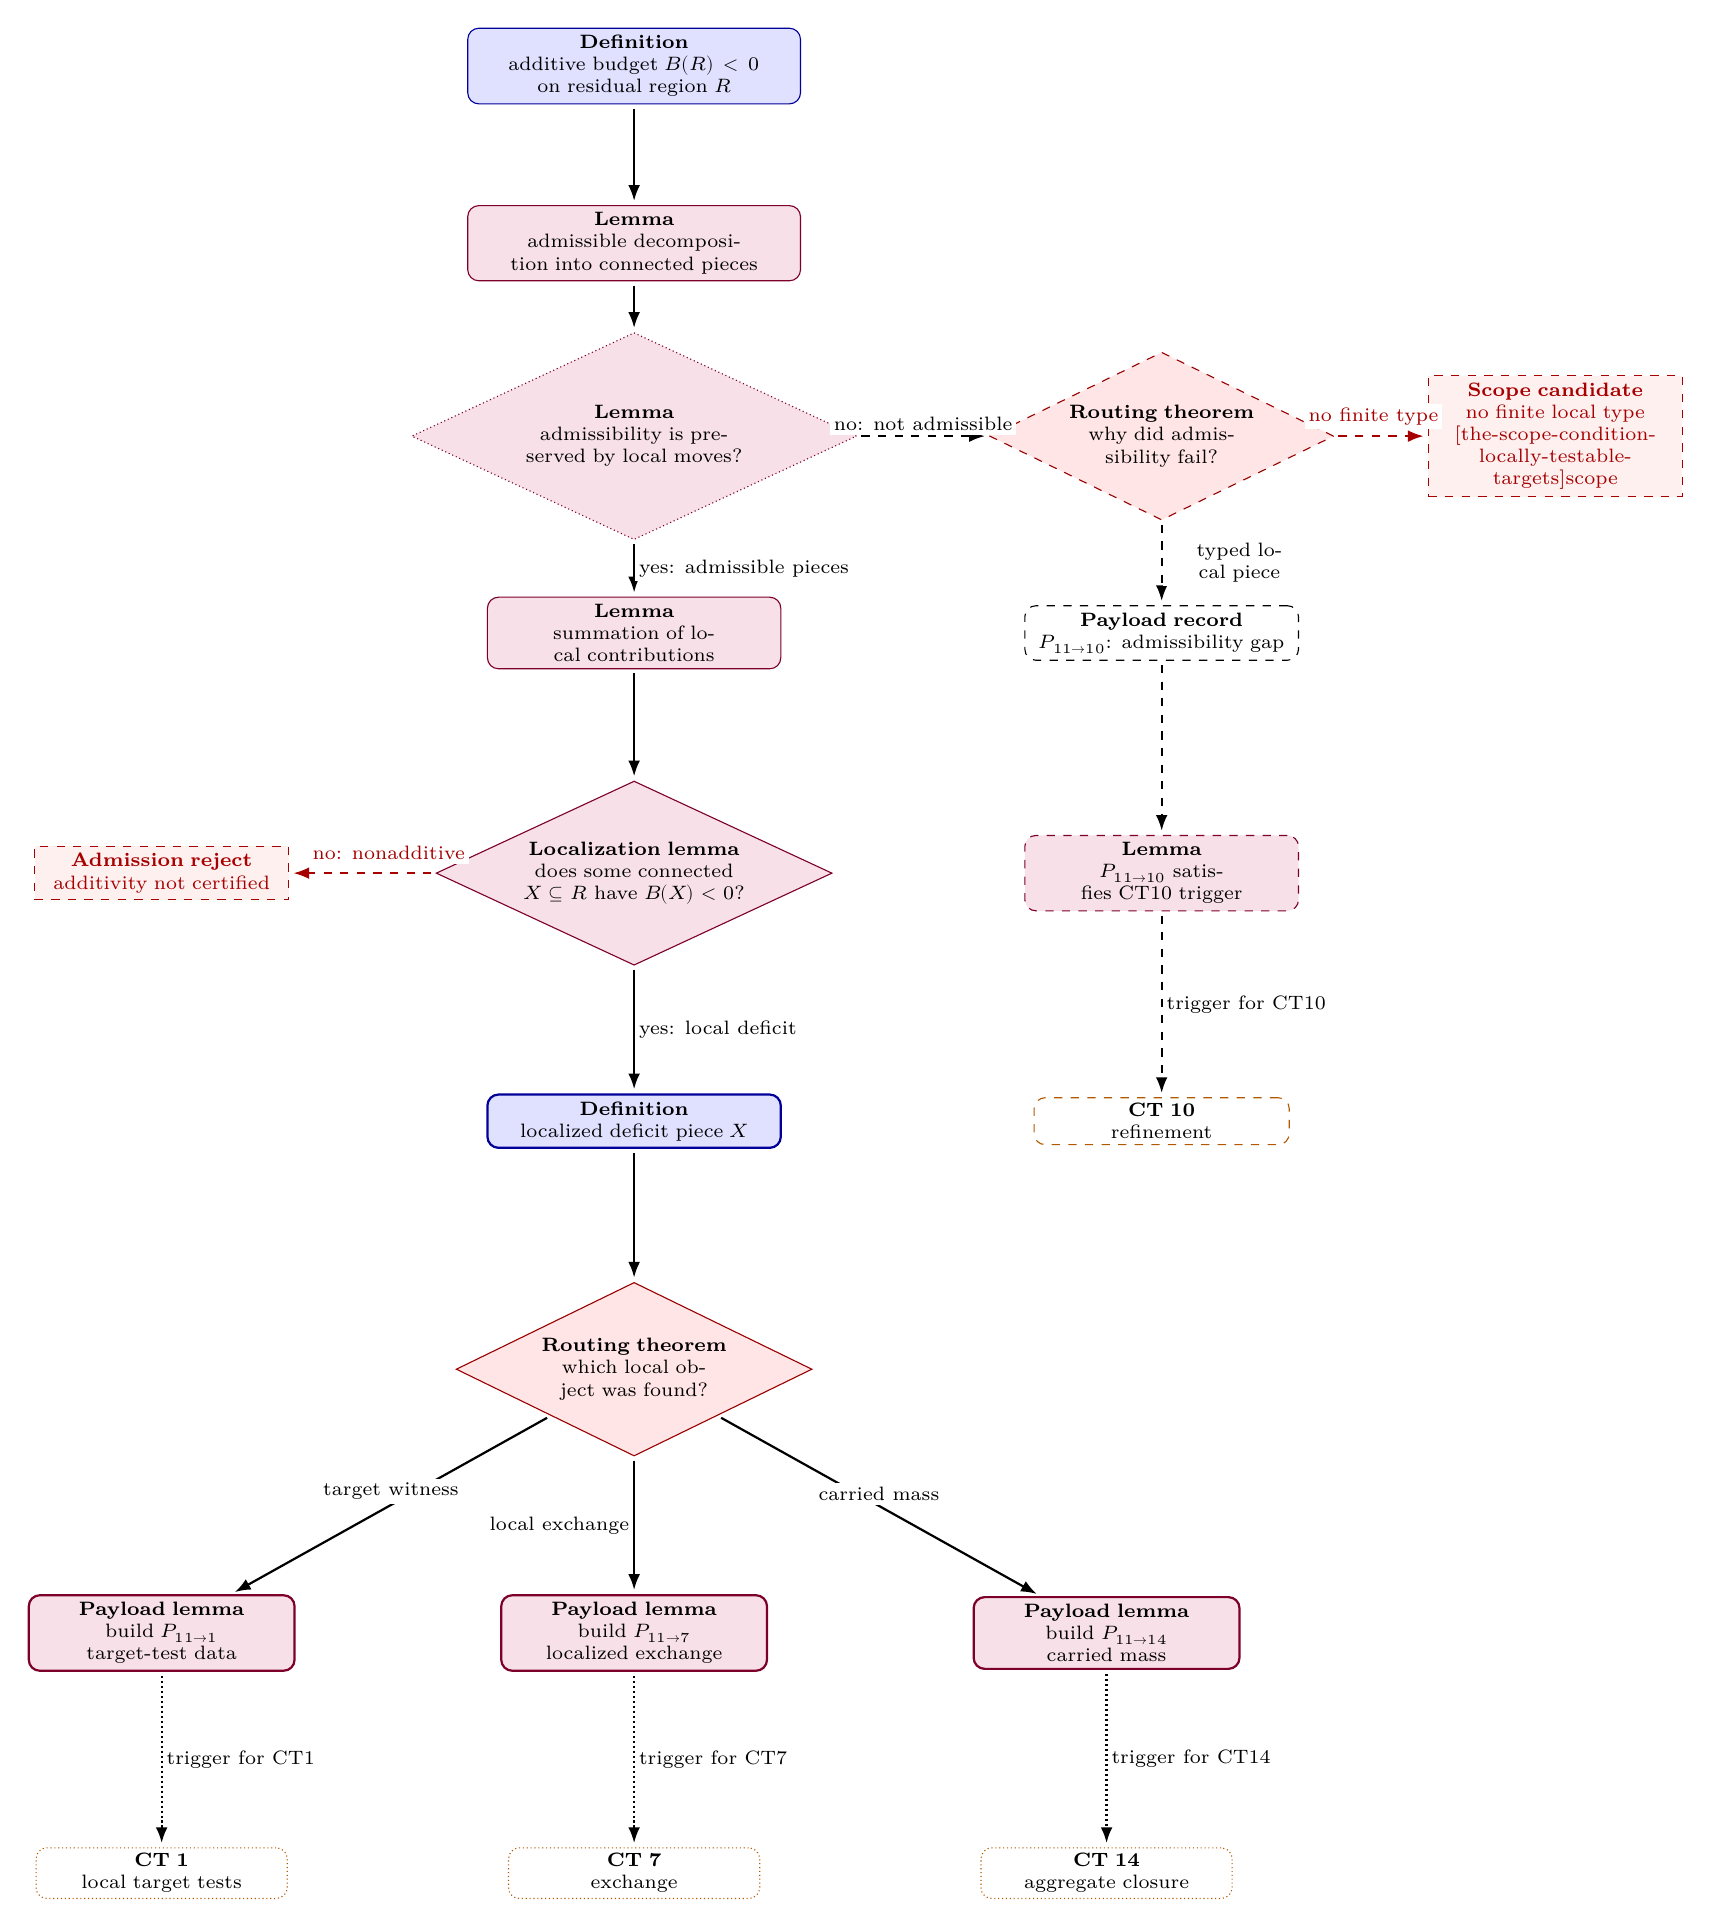
\begin{tikzpicture}[
every node/.style={font=\scriptsize}
]
\node[bcwide,bcdefinition] (input) at (0,0) {\textbf{Definition}\\additive budget \(B(R)<0\) on residual region \(R\)};
\node[bcwide,bclemma] (decomp) at (0,-2.25) {\textbf{Lemma}\\admissible decomposition into connected pieces};
\node[bcauditbox,text width=3.75cm,minimum width=3.75cm] (closed) at (0,-4.70) {\textbf{Lemma}\\admissibility is preserved by local moves?};
\node[bcroutechoice,bctheorem,bcdesign,text width=2.55cm,minimum width=3.15cm] (toolroute) at (6.70,-4.70) {\textbf{Routing theorem}\\why did admissibility fail?};
\node[bcscopefail,text width=3.05cm,minimum width=3.05cm] (bad) at (11.70,-4.70) {\textbf{Scope candidate}\\no finite local type\\\scoperef};
\node[bcbox,bclemma,text width=3.55cm,minimum width=3.55cm] (sum) at (0,-7.20) {\textbf{Lemma}\\summation of local contributions};
\node[bcbox,bcdesign,text width=3.30cm,minimum width=3.30cm] (toolres) at (6.70,-7.20) {\textbf{Payload record}\\\(P_{11\to10}\): admissibility gap};
\node[bcdec,bclemma,text width=3.10cm,minimum width=3.95cm] (local) at (0,-10.25) {\textbf{Localization lemma}\\does some connected \(X\subseteq R\) have \(B(X)<0\)?};
\node[bcscopefail,text width=3.05cm,minimum width=3.05cm] (badlocal) at (-6.00,-10.25) {\textbf{Admission reject}\\additivity not certified};
\node[bcbox,bclemma,bcdesign,text width=3.30cm,minimum width=3.30cm] (toollemma) at (6.70,-10.25) {\textbf{Lemma}\\\(P_{11\to10}\) satisfies CT10 trigger};
\node[bcbox,bcdefinition,bcpayload,text width=3.55cm,minimum width=3.55cm] (object) at (0,-13.40) {\textbf{Definition}\\localized deficit piece \(X\)};
\node[bcroute,bcrouteneutral,bcdesign,text width=3.10cm,minimum width=3.10cm] (toolfix) at (6.70,-13.40) {\textbf{CT 10}\\refinement};
\node[bcroutechoice,bctheorem,text width=2.70cm,minimum width=3.35cm] (nextroute) at (0,-16.55) {\textbf{Routing theorem}\\which local object was found?};
\node[bcbox,bclemma,bcpayload,text width=3.20cm,minimum width=3.20cm] (targetlemma) at (-6.00,-19.90) {\textbf{Payload lemma}\\build \(P_{11\to1}\)\\target-test data};
\node[bcbox,bclemma,bcpayload,text width=3.20cm,minimum width=3.20cm] (exchangelemma) at (0,-19.90) {\textbf{Payload lemma}\\build \(P_{11\to7}\)\\localized exchange};
\node[bcbox,bclemma,bcpayload,text width=3.20cm,minimum width=3.20cm] (aggregatelemma) at (6.00,-19.90) {\textbf{Payload lemma}\\build \(P_{11\to14}\)\\carried mass};
\node[bcroute,bcrouteneutral,bcoutputroute,text width=3.05cm,minimum width=3.05cm] (targetroute) at (-6.00,-22.95) {\textbf{CT 1}\\local target tests};
\node[bcroute,bcrouteneutral,bcoutputroute,text width=3.05cm,minimum width=3.05cm] (exchangeroute) at (0,-22.95) {\textbf{CT 7}\\exchange};
\node[bcroute,bcrouteneutral,bcoutputroute,text width=3.05cm,minimum width=3.05cm] (aggregateroute) at (6.00,-22.95) {\textbf{CT 14}\\aggregate closure};
\draw[bcarr] (input)--(decomp);
\draw[bcarr] (decomp)--(closed);
\draw[bcrecoverarr] (closed)--node[bclabel,above]{no: not admissible}(toolroute);
\draw[bcscopearr] (toolroute)--node[bclabel,above,pos=.42,yshift=2pt]{no finite type}(bad);
\draw[bcrecoverarr] (toolroute)--node[bclabel,right,text width=1.85cm,align=center]{typed local piece}(toolres);
\draw[bcrecoverarr] (toolres)--(toollemma);
\draw[bcrecoverarr] (toollemma)--node[bclabel,right]{trigger for CT10}(toolfix);
\draw[bcarr] (closed)--node[bclabel,right]{yes: admissible pieces}(sum);
\draw[bcarr] (sum)--(local);
\draw[bcarr] (local)--node[bclabel,right]{yes: local deficit}(object);
\draw[bcscopearr] (local)--node[bclabel,above,pos=.32,yshift=3pt]{no: nonadditive}(badlocal);
\draw[bcarr] (object)--(nextroute);
\draw[bcarr] (nextroute)--node[bclabel,above]{target witness}(targetlemma);
\draw[bcarr] (nextroute)--node[bclabel,left]{local exchange}(exchangelemma);
\draw[bcarr] (nextroute)--node[bclabel,above]{carried mass}(aggregatelemma);
\draw[bchandoff] (targetlemma)--node[bclabel,right]{trigger for CT1}(targetroute);
\draw[bchandoff] (exchangelemma)--node[bclabel,right]{trigger for CT7}(exchangeroute);
\draw[bchandoff] (aggregatelemma)--node[bclabel,right]{trigger for CT14}(aggregateroute);
\end{tikzpicture}%
}
\caption[Closure-tactic 11: localization lemma]{Closure-tactic 11 (localization lemma).  The tactic is certified by an additive-budget definition, an admissible-decomposition lemma, an admissibility lemma, a summation lemma, the localization lemma itself, a localized-deficit-piece definition, and payload lemmas routing the piece to target tests, exchange, or aggregate closure.  A typed admissibility gap constructs \(P_{11\to10}\); a localized target witness constructs \(P_{11\to1}\); a localized exchange constructs \(P_{11\to7}\); and carried mass constructs \(P_{11\to14}\).  Absence of finite local type data is a candidate scope obstruction referred to the global audit in \secref{the-scope-condition-locally-testable-targets}.  Line grammar (Fig.~\ref{fig:line-grammar-legend}): solid --- intended execution through the construction of the intended residual; dotted --- checks and the post-residual handoff to the consumer tactic; dashed --- design-failure recovery; red-dashed --- candidate scope obstruction referred to the global audit.}
\label{fig:ct11-localization}
\end{figure}
\FloatBarrier

\subsection*{Localization in practice}

Require every budget to be a sum of local contributions,

\[
B(X)\;=\;\sum_{v\in X} b(v)\;+\;\text{boundary corrections, bounded per attachment point.}
\]

Two consequences are then generic and are stated once, as lemmas, per
admissibility class:

\begin{enumerate}
\def\labelenumi{\arabic{enumi}.}
\tightlist
\item
  \emph{Summation}: global bounds are sums of local bounds, so the
  capacity inequality of the branch is the sum of per-cell inequalities.
\item
  \textbf{Localization}: if the aggregate budget is in deficit,
  \(B(R)<0\), then some \emph{connected admissible piece}
  \(X\subseteq R\) satisfies \(B(X)<0\) --- by decomposing \(R\) into
  connected admissible pieces and averaging.
\end{enumerate}

The localization lemma is the standard bridge from the counting layer to
the local-exclusion layer: it converts a global numerical deficit into a
bounded local object, which is where the taxonomy of \secref{the-branch-taxonomy} takes
over. Its proof is uniform; the admissibility class is the variable
input. The design obligation is that \textbf{admissibility be closed
under the moves of the local analysis} --- deletion, peeling, quotient
--- so that the localized piece remains inside the toolbox.

The low-level diagram for CT11 is Fig.~\ref{fig:ct11-localization};
it makes the additive decomposition, admissibility audit,
localization lemma, and exits to CT1, CT7, CT10, and CT14 explicit.



\subsection{CT12 --- Peeling loop}\label{ct:12}\label{peeling-loops-closure-by-well-founded-recursion}
\ctsignature{\(\langle\mathfrak B,L,\mu,\text{routed load}\rangle
\to \ctcert{C4};\ \ctint{\ctnone};\ \ctrec{P_{12\to4},P_{12\to13}}\).}

Some branches are not closed by a single application of any tactic: the
state contains a receiver that is over capacity, the overload has a
legitimate route, but routing it once removes only part of the excess.
You typically reach CT12 from a saturation test inside CT4's discharge
step, when the defect route of CT3 or CT7 consumes exactly one unit of
routed load.  The peeling loop is the disciplined way to apply such an
exit repeatedly.

\ctpar{Fires when}
The recorded state contains a receiver or account whose load counter
\(L\) exceeds its declared capacity, together with a certified
single-unit exit whose payload format matches one unit of routed load.
Both the counter and the move's availability are read from the branch
state.

\ctpar{You supply}
Two objects are required.  First, the load \(L\), a nonnegative integer
computable from recorded ledger deposits and register entries.  Second,
the peel move, a single-unit consumption operation inherited from the
tactic that created the routed load.

\ctpar{Execution}
Write two lemmas.  The peel lemma states that if the saturated branch
state holds and \(L=k>0\), then one peel produces either the unsaturated
branch or the same saturated branch state with load \(k-1\).  Every
standing invariant reappears in the conclusion; restoration belongs
inside the lemma, not after it.  The wrapper is induction on \(k\), or
well-founded recursion with termination measure \(L\).  The unsaturated
branch then closes by its discharge inequality, a C4 certificate supplied
by the surrounding charging argument.

\ctpar{Soundness obligations}
\begin{itemize}
\tightlist
\item \textbf{definition} is instantiated with the routed load account, the peel move, and the measure \(L\).
\item \textbf{S-Det} is instantiated with the canonical choice of the eligible unit peeled on each non-closing pass.
\item \textbf{S-Rest} is instantiated with the transition from the pre-peel branch state to the restored post-peel branch state.
\item \textbf{S-Meas} is instantiated with the proof that \(L\) is defined from recorded data, takes values in the nonnegative integers, and decreases on every non-closing pass.
\item \textbf{composition} is instantiated with the termination or discharge comparison that closes the unsaturated branch.
\item \textbf{routing} is instantiated with \(P_{12\to4}\) and \(P_{12\to13}\) for ordinary charge demand and tier-interaction demand.
\item \textbf{trigger} is instantiated with the CT4 and CT13 triggers for demand created by a peel pass.
\end{itemize}

\ctpar{Routing}
The loop edge returns to the saturation test with the load decremented.
The unsaturated branch closes by C4.  If a pass spawns demand that cannot
be charged in the same pass, the demand is routed to CT4 as an ordinary
charge obligation or to CT13 as a tier interaction.

\ctpar{Limit}
CT12 is inapplicable when the proposed load is not a function of recorded
data; admission requires a recorded decreasing measure. The execution
error is skipping S-Rest; the defect register records CT12/S-Rest.

\begin{figure}[p]
\centering
\vspace*{-2.80cm}
\resizebox{0.98\textwidth}{!}{%
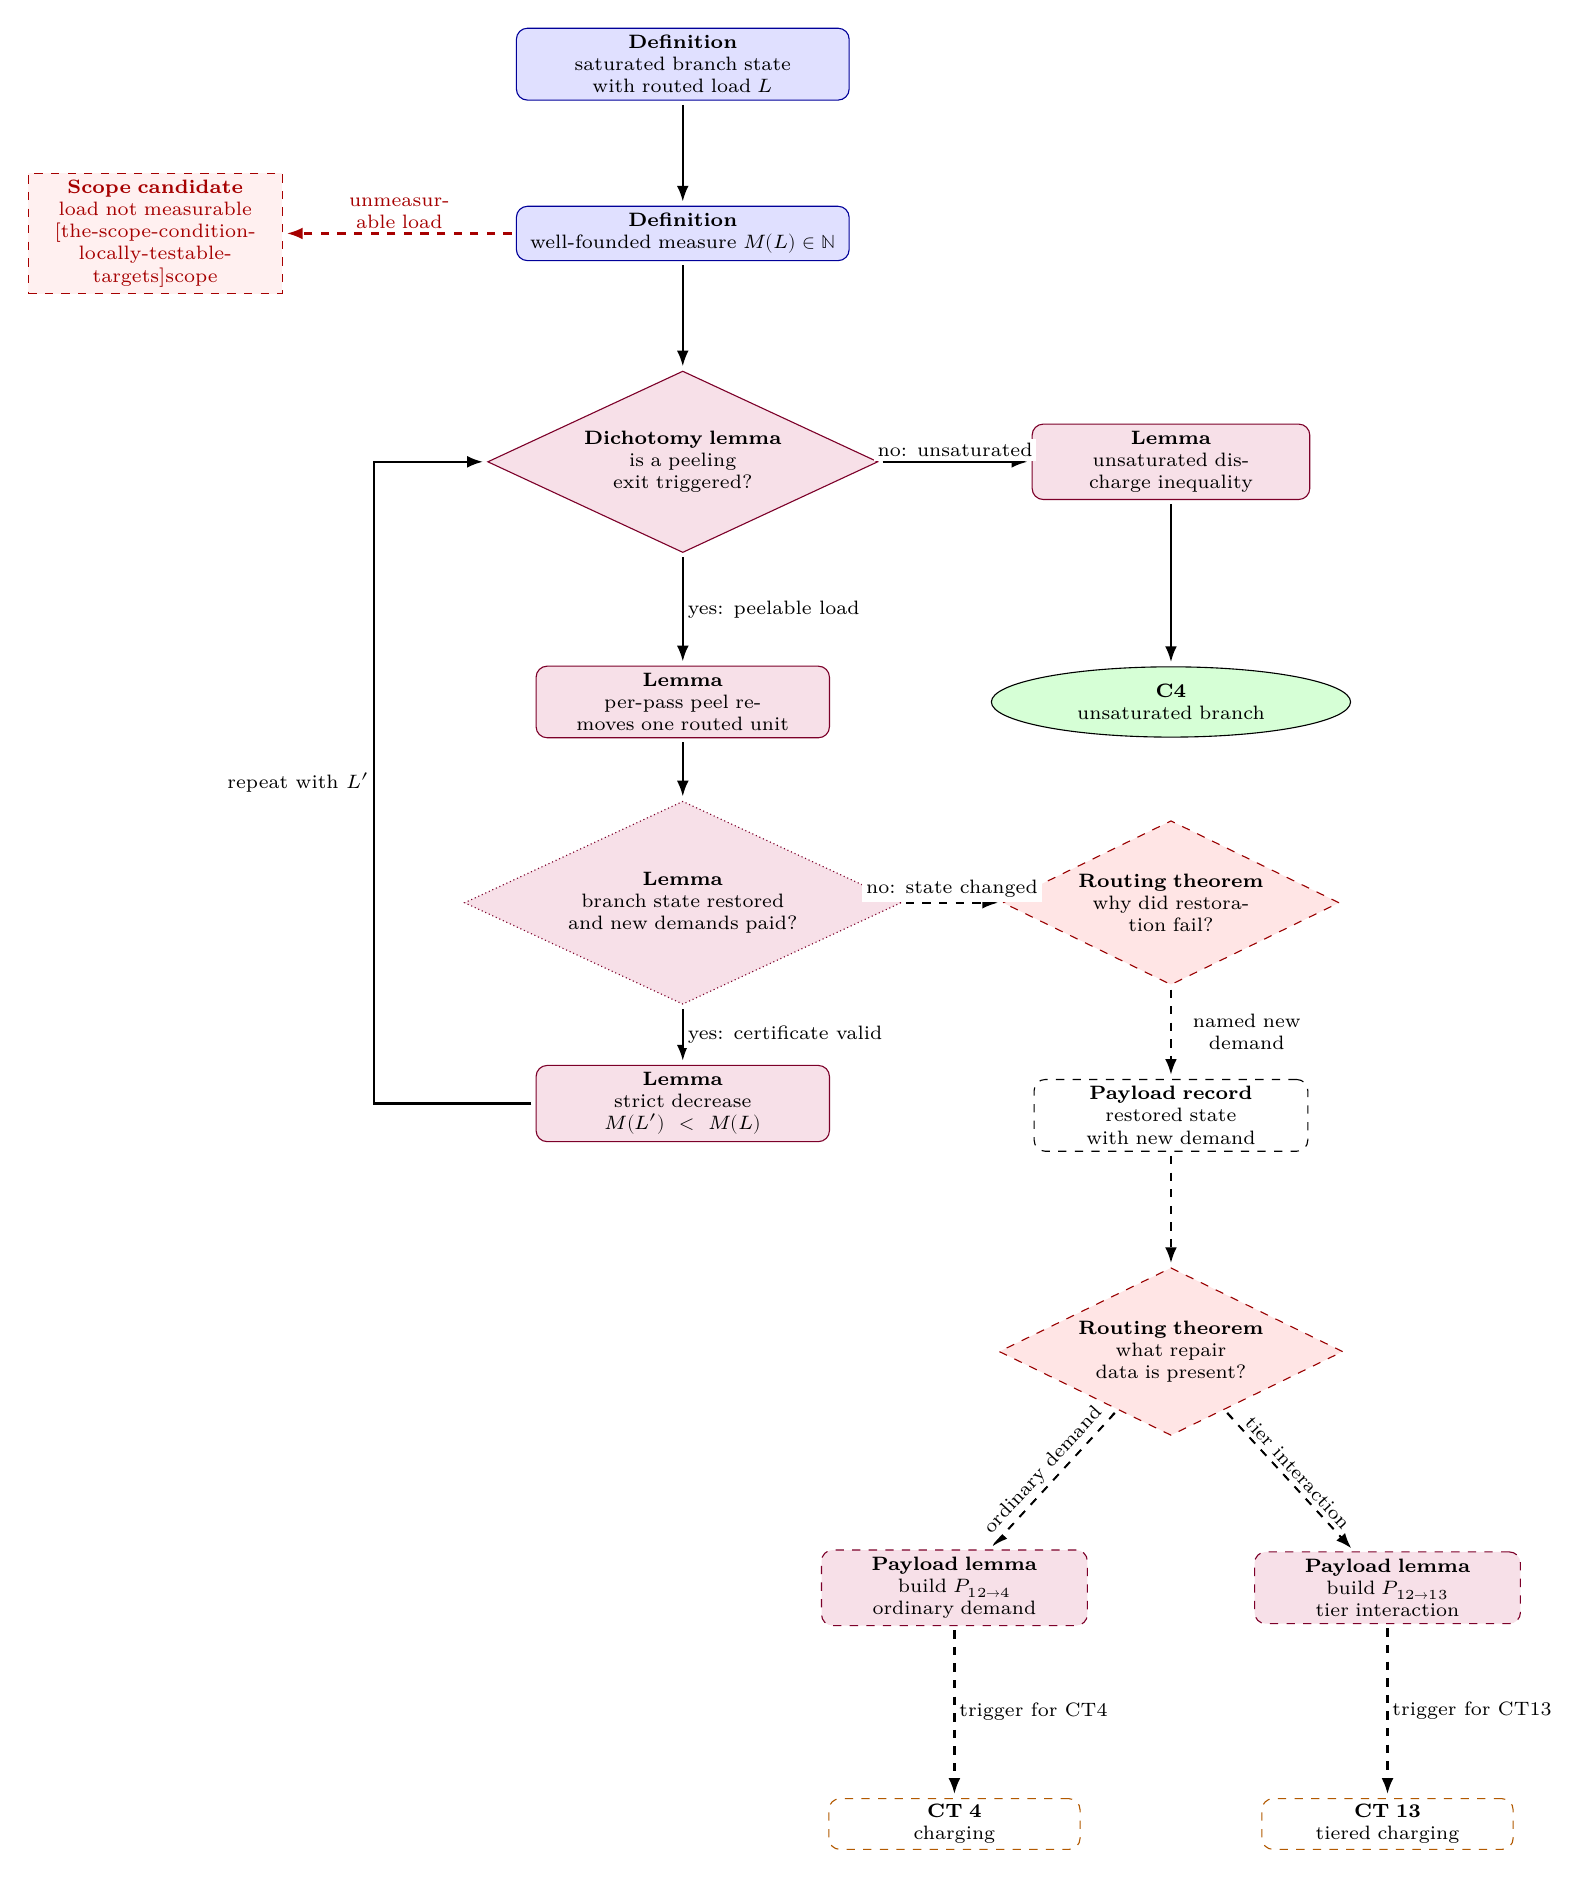
\begin{tikzpicture}[
every node/.style={font=\scriptsize}
]
\node[bcwide,bcdefinition] (input) at (0,0) {\textbf{Definition}\\saturated branch state with routed load \(L\)};
\node[bcwide,bcdefinition] (measuredef) at (0,-2.15) {\textbf{Definition}\\well-founded measure \(M(L)\in\mathbb N\)};
\node[bcdec,bclemma,text width=3.05cm,minimum width=3.85cm] (sat) at (0,-5.05) {\textbf{Dichotomy lemma}\\is a peeling exit triggered?};
\node[bcbox,bclemma,text width=3.35cm,minimum width=3.35cm] (discharge) at (6.20,-5.05) {\textbf{Lemma}\\unsaturated discharge inequality};
\node[bcclosed,text width=3.05cm,minimum width=3.05cm] (unsat) at (6.20,-8.10) {\textbf{C4}\\unsaturated branch};
\node[bcbox,bclemma,text width=3.55cm,minimum width=3.55cm] (peel) at (0,-8.10) {\textbf{Lemma}\\per-pass peel removes one routed unit};
\node[bcauditbox,text width=3.65cm,minimum width=3.65cm] (restore) at (0,-10.65) {\textbf{Lemma}\\branch state restored and new demands paid?};
\node[bcscopefail,text width=3.05cm,minimum width=3.05cm] (scopebad) at (-6.70,-2.15) {\textbf{Scope candidate}\\load not measurable\\\scoperef};
\node[bcroutechoice,bctheorem,bcdesign,text width=2.55cm,minimum width=3.15cm] (restorefail) at (6.20,-10.65) {\textbf{Routing theorem}\\why did restoration fail?};
\node[bcbox,bclemma,text width=3.55cm,minimum width=3.55cm] (measure) at (0,-13.20) {\textbf{Lemma}\\strict decrease \(M(L')<M(L)\)};
\node[bcbox,bcdesign,text width=3.30cm,minimum width=3.30cm] (statefix) at (6.20,-13.35) {\textbf{Payload record}\\restored state with new demand};
\node[bcroutechoice,bctheorem,bcdesign,text width=2.55cm,minimum width=3.15cm] (repairroute) at (6.20,-16.35) {\textbf{Routing theorem}\\what repair data is present?};
\node[bcbox,bclemma,bcdesign,text width=3.20cm,minimum width=3.20cm] (chargelemma) at (3.45,-19.35) {\textbf{Payload lemma}\\build \(P_{12\to4}\)\\ordinary demand};
\node[bcbox,bclemma,bcdesign,text width=3.20cm,minimum width=3.20cm] (tierlemma) at (8.95,-19.35) {\textbf{Payload lemma}\\build \(P_{12\to13}\)\\tier interaction};
\node[bcroute,bcrouteneutral,bcdesign,text width=3.05cm,minimum width=3.05cm] (chargeroute) at (3.45,-22.35) {\textbf{CT 4}\\charging};
\node[bcroute,bcrouteneutral,bcdesign,text width=3.05cm,minimum width=3.05cm] (tierroute) at (8.95,-22.35) {\textbf{CT 13}\\tiered charging};
\draw[bcarr] (input)--(measuredef);
\draw[bcarr] (measuredef)--(sat);
\draw[bcarr] (sat)--node[bclabel,above]{no: unsaturated}(discharge);
\draw[bcarr] (discharge)--(unsat);
\draw[bcarr] (sat)--node[bclabel,right]{yes: peelable load}(peel);
\draw[bcarr] (peel)--(restore);
\draw[bcscopearr] (measuredef.west)--node[bclabel,above,pos=.50,text width=2.05cm,align=center]{unmeasurable load}(scopebad.east);
\draw[bcrecoverarr] (restore)--node[bclabel,above]{no: state changed}(restorefail);
\draw[bcrecoverarr] (restorefail)--node[bclabel,right,text width=1.80cm,align=center]{named new demand}(statefix);
\draw[bcrecoverarr] (statefix)--(repairroute);
\draw[bcrecoverarr] (repairroute)--node[bclabel,above,sloped]{ordinary demand}(chargelemma);
\draw[bcrecoverarr] (repairroute)--node[bclabel,above,sloped]{tier interaction}(tierlemma);
\draw[bcrecoverarr] (chargelemma)--node[bclabel,right]{trigger for CT4}(chargeroute);
\draw[bcrecoverarr] (tierlemma)--node[bclabel,right]{trigger for CT13}(tierroute);
\draw[bcarr] (restore)--node[bclabel,right]{yes: certificate valid}(measure);
\draw[bcloop] (measure.west) -- ++(-2.05,0) |- node[bclabel,pos=.25,left]{repeat with \(L'\)} (sat.west);
\end{tikzpicture}%
}
\caption[Closure-tactic 12: peeling loops]{Closure-tactic 12 (peeling loops).  The tactic consumes a routed defect/load account, including peelable loads emitted by external-type compression or exchange trichotomy.  It requires definitions of the saturated load and well-founded measure, a peeling-exit dichotomy lemma, an unsaturated discharge lemma, a per-pass peel lemma, a restoration lemma, and a strict-decrease lemma whose loop terminates at the C4 unsaturated discharge.  A restored ordinary demand constructs \(P_{12\to4}\), while a tier interaction constructs \(P_{12\to13}\); a load not measurable from the branch state is a candidate scope obstruction referred to the global audit in \secref{the-scope-condition-locally-testable-targets}.  Line grammar (Fig.~\ref{fig:line-grammar-legend}): solid --- intended execution through the construction of the intended residual; dotted --- checks and the post-residual handoff to the consumer tactic; dashed --- design-failure recovery; red-dashed --- candidate scope obstruction referred to the global audit.}
\label{fig:ct12-peeling-loop}
\end{figure}
\FloatBarrier

\subsection{CT13 --- Tiered charging}\label{ct:13}\label{tiered-charging-scheme-failure-as-a-demand}
\ctsignature{\(P_{\ast\to13}\to \ctcert{C4};\ \ctint{P_{13\to4},P_{13\to9},P_{13\to14}};\ \ctrec{\ctnone}\).}

You reach CT13 when an ordinary charging account is conditional on an
availability hypothesis, and failure of that hypothesis creates a new
structured demand.  The tactic turns the failure of one scheme into the
input of a fallback scheme.

\ctpar{Fires when}
The state records a first-tier account or an obstruction record together
with the tier-interaction data.

\ctpar{You supply}
You supply the tier split, the availability test, the minimal obstruction
definition, and the reconciliation rule for payer sets.

\ctpar{Execution}
State the tier-one availability hypothesis and prove the tier-one payment
lemma under that hypothesis.  On the complementary branch, define the
minimal obstruction to availability using the declared size order and
tie-breaking rule.  The obstruction determines the tier-two payer map:
each fallback demand records the obstruction that created it and the
payer selected by the canonical rule.  Prove determinism from
minimality and tie-breaking before any capacity comparison is used.  Then
reconcile tier-one and tier-two payer sets by a disjointness lemma or by
an explicit fractional split.  The combined capacity theorem closes by
C4 when the accounts reconcile; an unreconciled fibre constructs
\(P_{13\to9}\), and unreconciled aggregate mass constructs
\(P_{13\to14}\).

\ctpar{Soundness obligations}
\begin{itemize}
\tightlist
\item \textbf{definition} is instantiated with the tier-one account, the fallback tier data, and the availability hypothesis.
\item \textbf{S-Det} is instantiated with the tier assignments and the canonical minimal obstruction selected when availability fails.
\item \textbf{dichotomy} is instantiated with the alternatives that the tier-one scheme is available or a fallback obstruction must be charged.
\item \textbf{composition} is instantiated with the reconciliation lemma and the combined tier-capacity comparison.
\item \textbf{routing} is instantiated with \(P_{13\to4}\), \(P_{13\to9}\), and \(P_{13\to14}\) for tier-one accounts, overlap fibres, and overlap mass.
\item \textbf{trigger} is instantiated with the CT4, CT9, and CT14 triggers for those tiered-charging outputs.
\end{itemize}

\ctpar{Routing}
Reconciled tiers close by C4.  A tier-one account routes to CT4, an
overlap fibre routes to CT9, and overlap mass routes to CT14.

\ctpar{Limit}
CT13 is inapplicable when no measurable tier resource is available. The
execution error is an unrecorded tier overlap; the audit records
CT13/S-Det or CT13/routing.

\begin{figure}[p]
\centering
\vspace*{-2.80cm}
\resizebox{0.95\textwidth}{!}{%
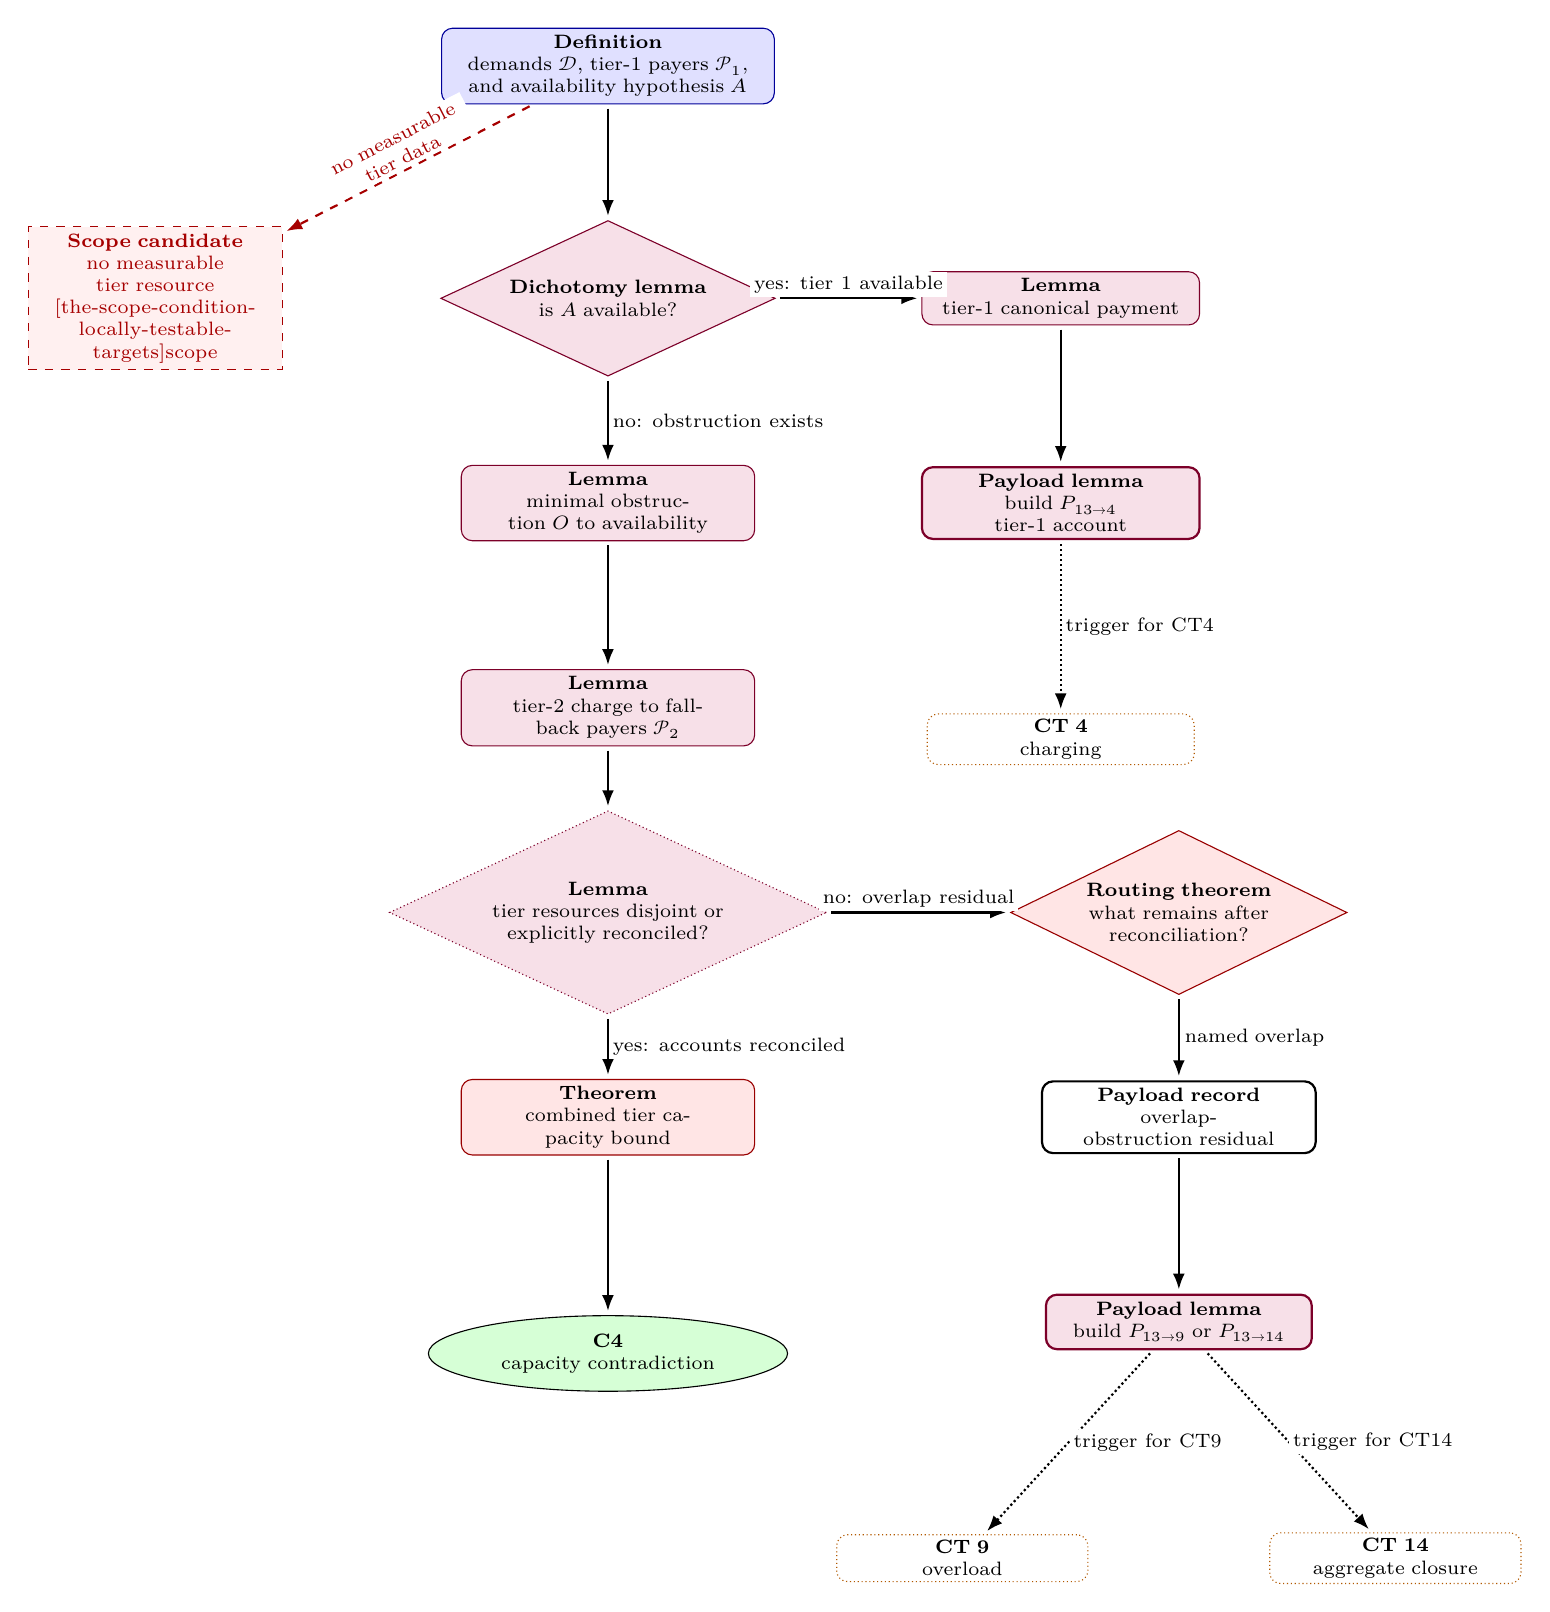
\begin{tikzpicture}[
every node/.style={font=\scriptsize}
]
\node[bcwide,bcdefinition] (input) at (0,0) {\textbf{Definition}\\demands \(\mathcal D\), tier-1 payers \(\mathcal P_1\), and availability hypothesis \(A\)};
\node[bcscopefail,text width=3.05cm,minimum width=3.05cm] (scopebad) at (-5.75,-2.95) {\textbf{Scope candidate}\\no measurable tier resource\\\scoperef};
\node[bcdec,bclemma,text width=3.05cm,minimum width=3.85cm] (avail) at (0,-2.95) {\textbf{Dichotomy lemma}\\is \(A\) available?};
\node[bcbox,bclemma,text width=3.35cm,minimum width=3.35cm] (tierone) at (5.75,-2.95) {\textbf{Lemma}\\tier-1 canonical payment};
\node[bcbox,bclemma,bcpayload,text width=3.35cm,minimum width=3.35cm] (capone) at (5.75,-5.55) {\textbf{Payload lemma}\\build \(P_{13\to4}\)\\tier-1 account};
\node[bcroute,bcrouteneutral,bcoutputroute,text width=3.25cm,minimum width=3.25cm] (caproute) at (5.75,-8.55) {\textbf{CT 4}\\charging};
\node[bcbox,bclemma,text width=3.55cm,minimum width=3.55cm] (minobs) at (0,-5.55) {\textbf{Lemma}\\minimal obstruction \(O\) to availability};
\node[bcbox,bclemma,text width=3.55cm,minimum width=3.55cm] (tiertwo) at (0,-8.15) {\textbf{Lemma}\\tier-2 charge to fallback payers \(\mathcal P_2\)};
\node[bcauditbox,text width=3.65cm,minimum width=3.65cm] (reconcile) at (0,-10.75) {\textbf{Lemma}\\tier resources disjoint or explicitly reconciled?};
\node[bcroutechoice,bctheorem,text width=2.55cm,minimum width=3.15cm] (overlaproute) at (7.25,-10.75) {\textbf{Routing theorem}\\what remains after reconciliation?};
\node[bcbox,bctheorem,text width=3.55cm,minimum width=3.55cm] (combined) at (0,-13.35) {\textbf{Theorem}\\combined tier capacity bound};
\node[bcbox,bcpayload,text width=3.30cm,minimum width=3.30cm] (overlapres) at (7.25,-13.35) {\textbf{Payload record}\\overlap-obstruction residual};
\node[bcbox,bclemma,bcpayload,text width=3.20cm,minimum width=3.20cm] (overlaplemma) at (7.25,-15.95) {\textbf{Payload lemma}\\build \(P_{13\to9}\) or \(P_{13\to14}\)};
\node[bcclosed,text width=3.05cm,minimum width=3.05cm] (captwo) at (0,-16.35) {\textbf{C4}\\capacity contradiction};
\node[bcroute,bcrouteneutral,bcoutputroute,text width=3.05cm,minimum width=3.05cm] (overroute) at (4.50,-18.95) {\textbf{CT 9}\\overload};
\node[bcroute,bcrouteneutral,bcoutputroute,text width=3.05cm,minimum width=3.05cm] (massroute) at (10.00,-18.95) {\textbf{CT 14}\\aggregate closure};
\draw[bcarr] (input)--(avail);
\draw[bcscopearr] (input)--node[bclabel,above,sloped,text width=1.95cm,align=center]{no measurable tier data}(scopebad);
\draw[bcarr] (avail)--node[bclabel,above]{yes: tier 1 available}(tierone);
\draw[bcarr] (tierone)--(capone);
\draw[bchandoff] (capone)--node[bclabel,right]{trigger for CT4}(caproute);
\draw[bcarr] (avail)--node[bclabel,right]{no: obstruction exists}(minobs);
\draw[bcarr] (minobs)--(tiertwo);
\draw[bcarr] (tiertwo)--(reconcile);
\draw[bcarr] (reconcile)--node[bclabel,above]{no: overlap residual}(overlaproute);
\draw[bcarr] (overlaproute)--node[bclabel,right,text width=1.80cm,align=center]{named overlap}(overlapres);
\draw[bcarr] (overlapres)--(overlaplemma);
\draw[bchandoff] (overlaplemma)--node[bclabel,right]{trigger for CT9}(overroute);
\draw[bchandoff] (overlaplemma)--node[bclabel,right]{trigger for CT14}(massroute);
\draw[bcarr] (reconcile)--node[bclabel,right]{yes: accounts reconciled}(combined);
\draw[bcarr] (combined)--(captwo);
\end{tikzpicture}%
}
\caption[Closure-tactic 13: tiered charging]{Closure-tactic 13 (tiered charging).  The tactic requires definitions of the tier-one scheme and availability hypothesis, an availability dichotomy lemma, a tier-one payment lemma, a minimal-obstruction lemma for failure, a tier-two charging lemma, a reconciliation lemma, and a combined capacity theorem.  A successful tier-one account constructs \(P_{13\to4}\); a named overlap obstruction constructs \(P_{13\to9}\) when it is a fibre overload and \(P_{13\to14}\) when it is aggregate mass.  Absence of a measurable tier resource is a candidate scope obstruction referred to the global audit in \secref{the-scope-condition-locally-testable-targets}; empty-rate recovery before admission belongs to \secref{nondeterminism-inventory}.  Line grammar (Fig.~\ref{fig:line-grammar-legend}): solid --- intended execution through the construction of the intended residual; dotted --- checks and the post-residual handoff to the consumer tactic; dashed --- design-failure recovery; red-dashed --- candidate scope obstruction referred to the global audit.}
\label{fig:ct13-tiered-charging}
\end{figure}
\FloatBarrier

\subsection*{Tiered charging in practice}

The bounded-multiplicity principle of \secref{the-charging-principle-in-general-form} has a second-order
form. Some charging schemes are \emph{conditionally} available: they
require a disjointness, independence, or compatibility hypothesis that
may fail. The correct design is \textbf{tiered charging}. The
availability hypothesis becomes a dichotomy, and its failure produces a
\emph{canonical minimal obstruction}, meaning a smallest witness of the
incompatibility. That obstruction becomes a demand in a designated
fallback scheme with its own payers.

The pattern is:

\[
\begin{aligned}
\text{scheme available} &\Rightarrow \text{pay in tier 1};\\
\text{scheme fails} &\Rightarrow \text{minimal obstruction} \Rightarrow \text{pay in tier 2}.
\end{aligned}
\]

The closure certificate is the pair of capacity inequalities, one per
tier, together with the minimality of the obstruction (which is what
makes the tier-2 assignment canonical). The reconciliation audit requires
the tier-2 payers to be disjoint from, or explicitly reconciled with, the
tier-1 payers; otherwise the two tiers double-charge the same resource.

The low-level diagram for CT13 is Fig.~\ref{fig:ct13-tiered-charging};
it shows the availability dichotomy, minimal obstruction, tier-two
account, reconciliation audit, and typed overlap exits.



\subsection{CT14 --- Aggregate closure}\label{ct:14}\label{aggregate-closure-mass-bounds-on-residual-classes}
\ctsignature{\(P_{\ast\to14}\to \ctcert{C4};\ \ctint{\ctnone};\ \ctrec{P_{14\to9},P_{14\to10}}\).}

CT14 consumes a typed residual class with a forced-mass lower bound and a
class-capacity record.  The tactic compares that lower bound with a
sublinear or bounded-capacity upper bound.

\ctpar{Fires when}
The state records a residual class, a lower mass estimate, and a
candidate capacity record for the class.

\ctpar{You supply}
You supply the class mass lower bound, the candidate per-member capacity
classifier, and the aggregate upper-bound record.

\ctpar{Execution}
Define the residual class together with the branch state under which its
members are counted.  Prove the lower-mass lemma: the surviving branch
forces \(\mathcal C\) to carry at least \(cn-o(n)\) units of deficit or
demand.  Separately prove the per-member capacity lemma, including the
maximum multiplicity with which a member may carry charge.  Sum the
member capacities with that carried-charge multiplicity to obtain the
aggregate upper bound \(o(n)\), or the recorded bounded-capacity variant.
The comparison theorem then places the lower and upper estimates in the
same units and gives C4.  If the upper bound fails because a named
member has unbounded capacity or unrecorded multiplicity, package that
member as \(P_{14\to9}\).  If the audit instead exposes a bounded missing
capacity-classification datum, package the residual class and datum as
\(P_{14\to10}\).

\ctpar{Soundness obligations}
\begin{itemize}
\tightlist
\item \textbf{definition} is instantiated with the residual class \(\mathcal C\), its recorded branch state, and the mass and capacity records attached to the class.
\item \textbf{composition} is instantiated with the lower-mass estimate, upper-capacity estimate, carried-charge multiplicity bound, and final aggregate contradiction.
\item \textbf{routing} is instantiated with \(P_{14\to9}\) for a named unbounded-capacity member or multiplicity gap and \(P_{14\to10}\) for a bounded missing capacity-classification datum.
\item \textbf{trigger} is instantiated with the CT9 trigger for the unbounded-member overload payload and the CT10 trigger for finite capacity-label refinement.
\end{itemize}

\ctpar{Routing}
The comparison closes by C4.  A named unbounded-capacity member or
multiplicity gap routes to CT9.  A bounded missing capacity datum routes
to CT10 as \(P_{14\to10}\).

\ctpar{Limit}
A bounded missing capacity classifier yields \(P_{14\to10}\). CT14 is
inapplicable when no finitely describable bounded-capacity description is
available. The execution error is failing to record per-member
multiplicity; the audit records CT14/composition.

\begin{figure}[p]
\centering
\vspace*{-2.80cm}
\resizebox{0.98\textwidth}{!}{%
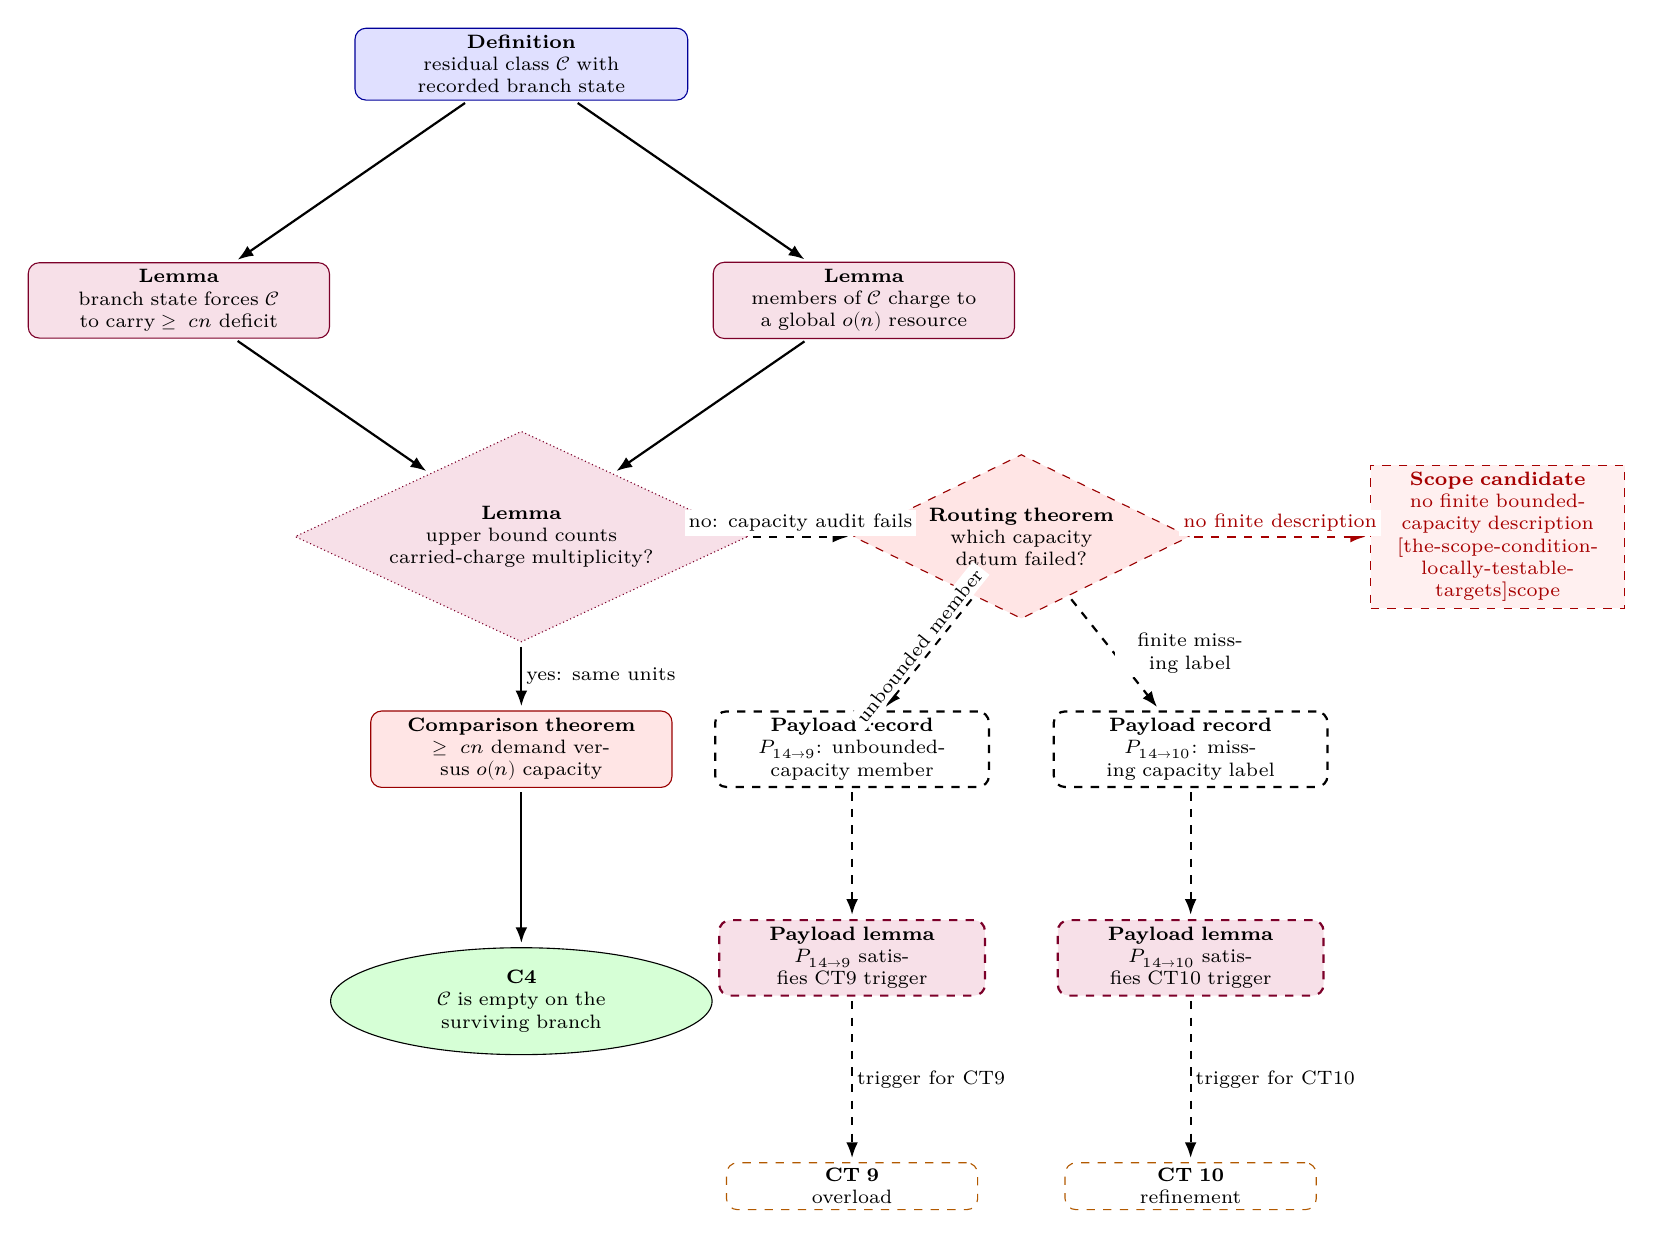
\begin{tikzpicture}[
every node/.style={font=\scriptsize}
]
\node[bcwide,bcdefinition] (input) at (0,0) {\textbf{Definition}\\residual class \(\mathcal C\) with recorded branch state};
\node[bcbox,bclemma,text width=3.65cm,minimum width=3.65cm] (lower) at (-4.35,-3.00) {\textbf{Lemma}\\branch state forces \(\mathcal C\) to carry \(\ge cn\) deficit};
\node[bcbox,bclemma,text width=3.65cm,minimum width=3.65cm] (upper) at (4.35,-3.00) {\textbf{Lemma}\\members of \(\mathcal C\) charge to a global \(o(n)\) resource};
\node[bcauditbox,text width=3.85cm,minimum width=3.85cm] (mult) at (0,-6.00) {\textbf{Lemma}\\upper bound counts carried-charge multiplicity?};
\node[bcroutechoice,bctheorem,bcdesign,text width=2.55cm,minimum width=3.15cm] (multroute) at (6.35,-6.00) {\textbf{Routing theorem}\\which capacity datum failed?};
\node[bcscopefail,text width=3.05cm,minimum width=3.05cm] (scopebad) at (12.40,-6.00) {\textbf{Scope candidate}\\no finite bounded-capacity description\\\scoperef};
\node[bcbox,bctheorem,text width=3.65cm,minimum width=3.65cm] (compare) at (0,-8.70) {\textbf{Comparison theorem}\\\(\ge cn\) demand versus \(o(n)\) capacity};
\node[bcbox,bcdesign,bcpayload,text width=3.30cm,minimum width=3.30cm] (unbounded) at (4.20,-8.70) {\textbf{Payload record}\\\(P_{14\to9}\): unbounded-capacity member};
\node[bcbox,bcdesign,bcpayload,text width=3.30cm,minimum width=3.30cm] (refine) at (8.50,-8.70) {\textbf{Payload record}\\\(P_{14\to10}\): missing capacity label};
\node[bcbox,bclemma,bcdesign,bcpayload,text width=3.20cm,minimum width=3.20cm] (overlemma) at (4.20,-11.35) {\textbf{Payload lemma}\\\(P_{14\to9}\) satisfies CT9 trigger};
\node[bcbox,bclemma,bcdesign,bcpayload,text width=3.20cm,minimum width=3.20cm] (refinelemma) at (8.50,-11.35) {\textbf{Payload lemma}\\\(P_{14\to10}\) satisfies CT10 trigger};
\node[bcclosed,text width=3.25cm,minimum width=3.25cm] (closed) at (0,-11.90) {\textbf{C4}\\\(\mathcal C\) is empty on the surviving branch};
\node[bcroute,bcrouteneutral,bcdesign,text width=3.05cm,minimum width=3.05cm] (overroute) at (4.20,-14.25) {\textbf{CT 9}\\overload};
\node[bcroute,bcrouteneutral,bcdesign,text width=3.05cm,minimum width=3.05cm] (refineroute) at (8.50,-14.25) {\textbf{CT 10}\\refinement};
\draw[bcarr] (input)--(lower);
\draw[bcarr] (input)--(upper);
\draw[bcarr] (lower)--(mult);
\draw[bcarr] (upper)--(mult);
\draw[bcrecoverarr] (mult)--node[bclabel,above]{no: capacity audit fails}(multroute);
\draw[bcrecoverarr] (multroute)--node[bclabel,above,sloped]{unbounded member}(unbounded);
\draw[bcrecoverarr] (multroute)--node[bclabel,right,text width=1.80cm,align=center]{finite missing label}(refine);
\draw[bcscopearr] (multroute)--node[bclabel,above]{no finite description}(scopebad);
\draw[bcrecoverarr] (unbounded)--(overlemma);
\draw[bcrecoverarr] (refine)--(refinelemma);
\draw[bcrecoverarr] (overlemma)--node[bclabel,right]{trigger for CT9}(overroute);
\draw[bcrecoverarr] (refinelemma)--node[bclabel,right]{trigger for CT10}(refineroute);
\draw[bcarr] (mult)--node[bclabel,right]{yes: same units}(compare);
\draw[bcarr] (compare)--(closed);
\end{tikzpicture}%
}
\caption[Closure-tactic 14: aggregate closure]{Closure-tactic 14 (aggregate closure).  The tactic is certified by a residual-class definition, a lower-bound lemma, an upper-capacity lemma, a carried-charge multiplicity lemma, and a comparison theorem proving that the surviving residual class is empty.  A named unbounded-capacity member or multiplicity gap constructs \(P_{14\to9}\) for overload exhaustion; a bounded missing capacity-classification datum constructs \(P_{14\to10}\) for finite refinement.  Absence of any finite bounded-capacity description is a candidate scope obstruction referred to the global audit in \secref{the-scope-condition-locally-testable-targets}.  Line grammar (Fig.~\ref{fig:line-grammar-legend}): solid --- intended execution through the construction of the intended residual; dotted --- checks and the post-residual handoff to the consumer tactic; dashed --- design-failure recovery; red-dashed --- candidate scope obstruction referred to the global audit.}
\label{fig:ct14-aggregate-closure}
\end{figure}
\FloatBarrier

\subsection*{Aggregate closure in practice}

A residual class \(\mathcal C\) that is required, by the branch state,
to carry a \emph{linear} deficit can be closed by proving that its total
\textbf{deficit-carrying capacity} is \emph{sublinear}. This capacity is
the aggregate mass of charge all members of \(\mathcal C\) can absorb
together. The certificate has two halves: a lower bound, where the
surviving branch forces \(\mathcal C\) to carry \(\ge cn\) deficit, and
an upper bound, where the members of \(\mathcal C\) are charged to a
global resource of size \(o(n)\). Thus their total capacity is \(o(n)\),
and the class is empty on the surviving branch.

The aggregate comparison applies to a residual class with a recorded
linear deficit, sublinear aggregate capacity, and per-member
multiplicity.  The upper bound counts members \emph{with multiplicity by
carried charge}; a sublinear number of members can still carry linear
mass if individual capacities are unbounded, so the per-member capacity
bound is part of the certificate.

The low-level diagram for CT14 is Fig.~\ref{fig:ct14-aggregate-closure};
it links the lower-bound lemma, upper-capacity lemma, multiplicity audit,
comparison theorem, and overload route.



\subsection{CT15 --- Rank forcing}\label{ct:15}\label{rank-forcing-charge-only-independent-coordinates}
\ctsignature{\(P_{\ast\to15}\to \ctcert{C4};\ \ctint{P_{15\to3},P_{15\to7},P_{15\to16},P_{15\to4}};\ \ctrec{\ctnone}\).}

You reach CT15 when many tests are available but only independent
target-relevant coordinates may be charged.  The tactic builds a rank
firewall before entropy or capacity is spent.

\ctpar{Fires when}
The state records a target-relative rank datum controlling the family of
coordinates to be charged.

\ctpar{You supply}
You supply the rank map, dependence classifier, and full-rank ledger.
The rank is defined from what the tests say about the target, not from
incidental linear algebra.

\ctpar{Execution}
Define the target-relative rank map and prove the target-meaning lemma
that identifies which rank drops affect the target predicate.  Apply the
rank-drop dichotomy.  A drop produces an explicit dependence witness,
which is classified by its support: boundary response data gives
\(P_{15\to3}\), same-interface movable data gives \(P_{15\to7}\), and
closed whole-object data gives \(P_{15\to16}\).  On the full-rank
branch, construct the ledger only on independent coordinates certified
by the rank firewall.  The full-rank charge lemma spends the entropy or
budget once and records the consumed coordinates.  The resulting
comparison closes by C4 when demand exceeds capacity; otherwise the
certified ledger is emitted as \(P_{15\to4}\).

\ctpar{Soundness obligations}
\begin{itemize}
\tightlist
\item \textbf{definition} is instantiated with the target-relative rank map, the dependence classifier, and the full-rank ledger.
\item \textbf{dichotomy} is instantiated with the rank-drop branch and the full-rank branch.
\item \textbf{composition} is instantiated with the rank-budget comparison on certified independent coordinates.
\item \textbf{routing} is instantiated with \(P_{15\to3}\), \(P_{15\to4}\), \(P_{15\to7}\), and \(P_{15\to16}\) for rank defects, full-rank ledgers, rank exchanges, and rank delocalization.
\item \textbf{trigger} is instantiated with the CT3, CT4, CT7, and CT16 triggers for those rank-forcing outputs.
\end{itemize}

\ctpar{Routing}
Rank-drop dependence routes to CT3, CT7, or CT16.  A full-rank ledger
routes to CT4 or closes by C4.

\ctpar{Limit}
CT15 is inapplicable when no finite target-relative rank is available. The
execution error is charging incidental rank; the audit records
CT15/definition.

\begin{figure}[p]
\centering
\vspace*{-2.80cm}
\resizebox{0.98\textwidth}{!}{%
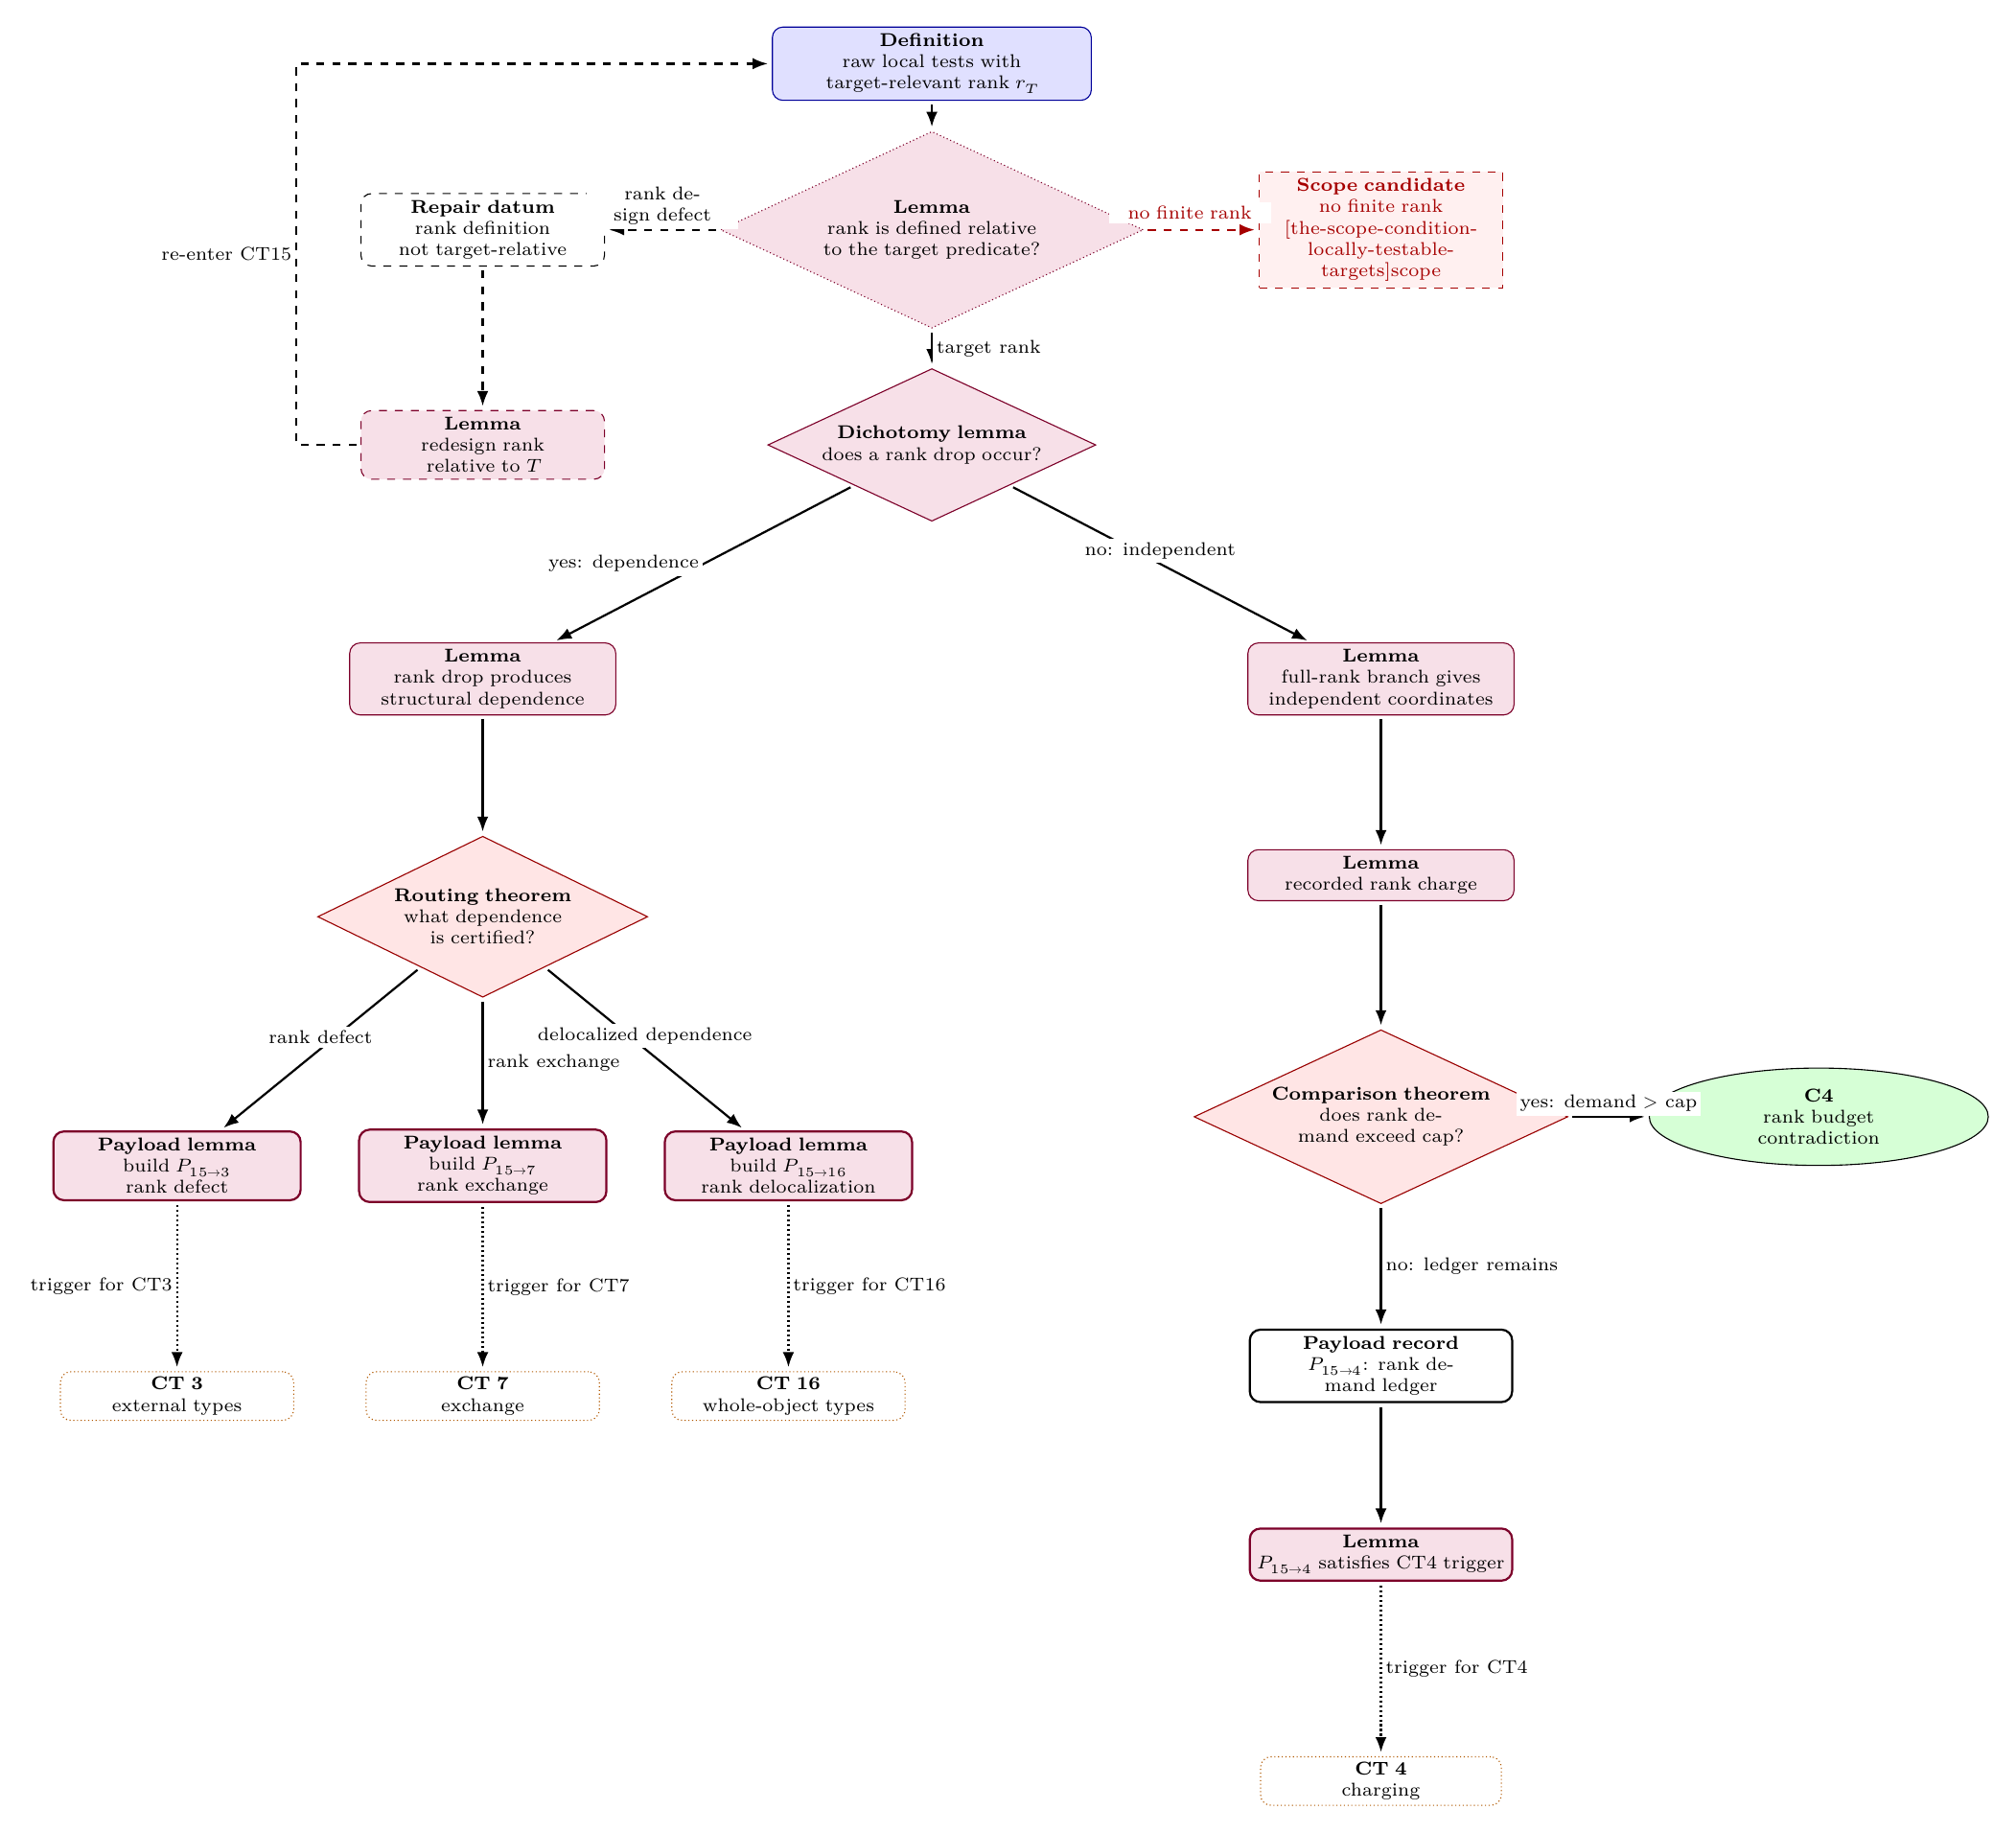
\begin{tikzpicture}[
every node/.style={font=\scriptsize}
]
\node[bcwide,bcdefinition] (input) at (0,0) {\textbf{Definition}\\raw local tests with target-relevant rank \(r_T\)};
\node[bcbox,bcdesign,text width=3.05cm,minimum width=3.05cm] (rankrepair) at (-5.95,-2.20) {\textbf{Repair datum}\\rank definition not target-relative};
\node[bcbox,bclemma,bcdesign,text width=3.05cm,minimum width=3.05cm] (rankrepairlemma) at (-5.95,-5.05) {\textbf{Lemma}\\redesign rank relative to \(T\)};
\node[bcauditbox,text width=3.70cm,minimum width=3.70cm] (targetaudit) at (0,-2.20) {\textbf{Lemma}\\rank is defined relative to the target predicate?};
\node[bcscopefail,text width=3.05cm,minimum width=3.05cm] (scopebad) at (5.95,-2.20) {\textbf{Scope candidate}\\no finite rank\\\scoperef};
\node[bcdec,bclemma,text width=3.05cm,minimum width=3.85cm] (rank) at (0,-5.05) {\textbf{Dichotomy lemma}\\does a rank drop occur?};
\node[bcbox,bclemma,text width=3.35cm,minimum width=3.35cm] (dep) at (-5.95,-8.15) {\textbf{Lemma}\\rank drop produces structural dependence};
\node[bcroutechoice,bctheorem,text width=2.65cm,minimum width=3.30cm] (structroute) at (-5.95,-11.30) {\textbf{Routing theorem}\\what dependence is certified?};
\node[bcbox,bclemma,bcpayload,text width=3.10cm,minimum width=3.10cm] (typelemma) at (-10.00,-14.60) {\textbf{Payload lemma}\\build \(P_{15\to3}\)\\rank defect};
\node[bcbox,bclemma,bcpayload,text width=3.10cm,minimum width=3.10cm] (exchangelemma) at (-5.95,-14.60) {\textbf{Payload lemma}\\build \(P_{15\to7}\)\\rank exchange};
\node[bcbox,bclemma,bcpayload,text width=3.10cm,minimum width=3.10cm] (wholelemma) at (-1.90,-14.60) {\textbf{Payload lemma}\\build \(P_{15\to16}\)\\rank delocalization};
\node[bcroute,bcrouteneutral,bcoutputroute,text width=2.95cm,minimum width=2.95cm] (typeroute) at (-10.00,-17.65) {\textbf{CT 3}\\external types};
\node[bcroute,bcrouteneutral,bcoutputroute,text width=2.95cm,minimum width=2.95cm] (exchangeroute) at (-5.95,-17.65) {\textbf{CT 7}\\exchange};
\node[bcroute,bcrouteneutral,bcoutputroute,text width=2.95cm,minimum width=2.95cm] (wholeroute) at (-1.90,-17.65) {\textbf{CT 16}\\whole-object types};
\node[bcbox,bclemma,text width=3.35cm,minimum width=3.35cm] (full) at (5.95,-8.15) {\textbf{Lemma}\\full-rank branch gives independent coordinates};
\node[bcbox,bclemma,text width=3.35cm,minimum width=3.35cm] (charge) at (5.95,-10.75) {\textbf{Lemma}\\recorded rank charge};
\node[bcdec,bctheorem,text width=3.05cm,minimum width=3.85cm] (compare) at (5.95,-13.95) {\textbf{Comparison theorem}\\does rank demand exceed cap?};
\node[bcclosed,text width=3.00cm,minimum width=3.00cm] (budget) at (11.75,-13.95) {\textbf{C4}\\rank budget contradiction};
\node[bcbox,bcpayload,text width=3.30cm,minimum width=3.30cm] (ledger) at (5.95,-17.25) {\textbf{Payload record}\\\(P_{15\to4}\): rank demand ledger};
\node[bcbox,bclemma,bcpayload,text width=3.30cm,minimum width=3.30cm] (chargelemma) at (5.95,-19.75) {\textbf{Lemma}\\\(P_{15\to4}\) satisfies CT4 trigger};
\node[bcroute,bcrouteneutral,bcoutputroute,text width=3.05cm,minimum width=3.05cm] (chargeroute) at (5.95,-22.75) {\textbf{CT 4}\\charging};
\draw[bcarr] (input)--(targetaudit);
\draw[bcscopearr] (targetaudit)--node[bclabel,above,pos=.40,yshift=2pt,text width=2.05cm,align=center]{no finite rank}(scopebad);
\draw[bcrecoverarr] (targetaudit)--node[bclabel,above,sloped,text width=1.90cm,align=center]{rank design defect}(rankrepair);
\draw[bcrecoverarr] (rankrepair)--(rankrepairlemma);
\draw[bcrecoverarr] (rankrepairlemma.west) -- ++(-0.85,0) |- node[bclabel,pos=.25,left]{re-enter CT15}(input.west);
\draw[bcarr] (targetaudit)--node[bclabel,right]{target rank}(rank);
\draw[bcarr] (rank)--node[bclabel,left]{yes: dependence}(dep);
\draw[bcarr] (dep)--(structroute);
\draw[bcarr] (structroute)--node[bclabel,above]{rank defect}(typelemma);
\draw[bcarr] (structroute)--node[bclabel,right]{rank exchange}(exchangelemma);
\draw[bcarr] (structroute)--node[bclabel,above]{delocalized dependence}(wholelemma);
\draw[bchandoff] (typelemma)--node[bclabel,left]{trigger for CT3}(typeroute);
\draw[bchandoff] (exchangelemma)--node[bclabel,right]{trigger for CT7}(exchangeroute);
\draw[bchandoff] (wholelemma)--node[bclabel,right]{trigger for CT16}(wholeroute);
\draw[bcarr] (rank)--node[bclabel,above]{no: independent}(full);
\draw[bcarr] (full)--(charge);
\draw[bcarr] (charge)--(compare);
\draw[bcarr] (compare)--node[bclabel,above]{yes: demand \(>\) cap}(budget);
\draw[bcarr] (compare)--node[bclabel,right]{no: ledger remains}(ledger);
\draw[bcarr] (ledger)--(chargelemma);
\draw[bchandoff] (chargelemma)--node[bclabel,right]{trigger for CT4}(chargeroute);
\end{tikzpicture}%
}
\caption[Closure-tactic 15: rank forcing]{Closure-tactic 15 (rank forcing).  The tactic is certified by a target-relative rank definition and target-meaning lemma, a rank-drop dichotomy lemma, a structural-dependence lemma, payload lemmas for \(P_{15\to3}\), \(P_{15\to7}\), and \(P_{15\to16}\), and full-rank charge and comparison lemmas that either close or route the ledger as \(P_{15\to4}\).  Redesigning the rank is a repairable design step; absence of a finite-description target-relative rank is a candidate scope obstruction referred to the global audit in \secref{the-scope-condition-locally-testable-targets}.  Line grammar (Fig.~\ref{fig:line-grammar-legend}): solid --- intended execution through the construction of the intended residual; dotted --- checks and the post-residual handoff to the consumer tactic; dashed --- design-failure recovery; red-dashed --- candidate scope obstruction referred to the global audit.}
\label{fig:ct15-rank-forcing}
\end{figure}
\FloatBarrier

\subsection*{Rank forcing in practice}

Raw local tests enter a counting or entropy bound after a rank-forcing
layer has removed dependencies. Define a target-relevant rank on the
family of tests, and split on rank deficiency. A rank drop is a
\emph{structural event} --- some dependence among tests --- and every
dependence is routed through the standard taxonomy: it is
target-defective, or it identifies pieces (compression), or it
delocalizes. On the complementary branch, the tests have full rank, and
then the forced cost

\[
(\text{cost per test}) \times (\text{number of tests})
\]

enters the budget as a recorded charge. Rank forcing is the accounting
firewall between structure and entropy: dependence is structure and is
routed; independence is entropy and is charged. The rank must be defined
relative to the \emph{target}, so that a rank drop carries routable
structural meaning.

The low-level diagram for CT15 is Fig.~\ref{fig:ct15-rank-forcing};
it displays the target-relative rank audit, rank-drop routing theorem,
full-rank charge, and ledger route.



\subsection{CT16 --- Whole-object exact types}\label{ct:16}\label{the-whole-object-piece-exact-types-under-context-degeneracy}
\ctsignature{\(P_{\ast\to16}\to \ctcert{C2};\ \ctint{P_{16\to3},P_{16\to10}};\ \ctrec{\ctnone}\).}

You reach CT16 when a neutral or rank-defect datum has support equal to
the whole object, so ordinary outside contexts have degenerated.  The
tactic replaces empty-context intuition by an exact closed type.

\ctpar{Fires when}
The state records a delocalized whole-object datum and a computable
closed-type slot.

\ctpar{You supply}
You supply the closed-type evaluator, the literal equality test, and the
proper-piece test.

\ctpar{Execution}
Represent the closed type as an explicit finite data structure. Prove a
no-silent-identification lemma: two whole-object data records are
identified only by literal equality of the computed closed type. If the
support is actually proper, leave the whole-object
tactic and return to ordinary external types.

\ctpar{Soundness obligations}
\begin{itemize}
\tightlist
\item \textbf{definition} is instantiated with the delocalized whole-object datum, the computable closed-type slot, and the literal equality test.
\item \textbf{equivalence} is instantiated with closed response equality and the no-silent-identification rule for the empty-context case.
\item \textbf{dichotomy} is instantiated with the split between proper support and whole-object support.
\item \textbf{routing} is instantiated with \(P_{16\to3}\) for proper-piece context data and \(P_{16\to10}\) for distinct closed data.
\item \textbf{trigger} is instantiated with the CT3 and CT10 triggers for the whole-object exits.
\end{itemize}

\ctpar{Routing}
Literal closed-type equality closes by C2.  A proper subpiece routes to
CT3.  Distinct closed data routes to CT10.

\ctpar{Limit}
CT16 is inapplicable when the required closed type is not finitely
computable. The execution error is identifying two whole-object records
solely because there is no nonempty outside context; the audit records
CT16/equivalence.

\begin{figure}[p]
\centering
\vspace*{-2.80cm}
\resizebox{!}{0.76\textheight}{%
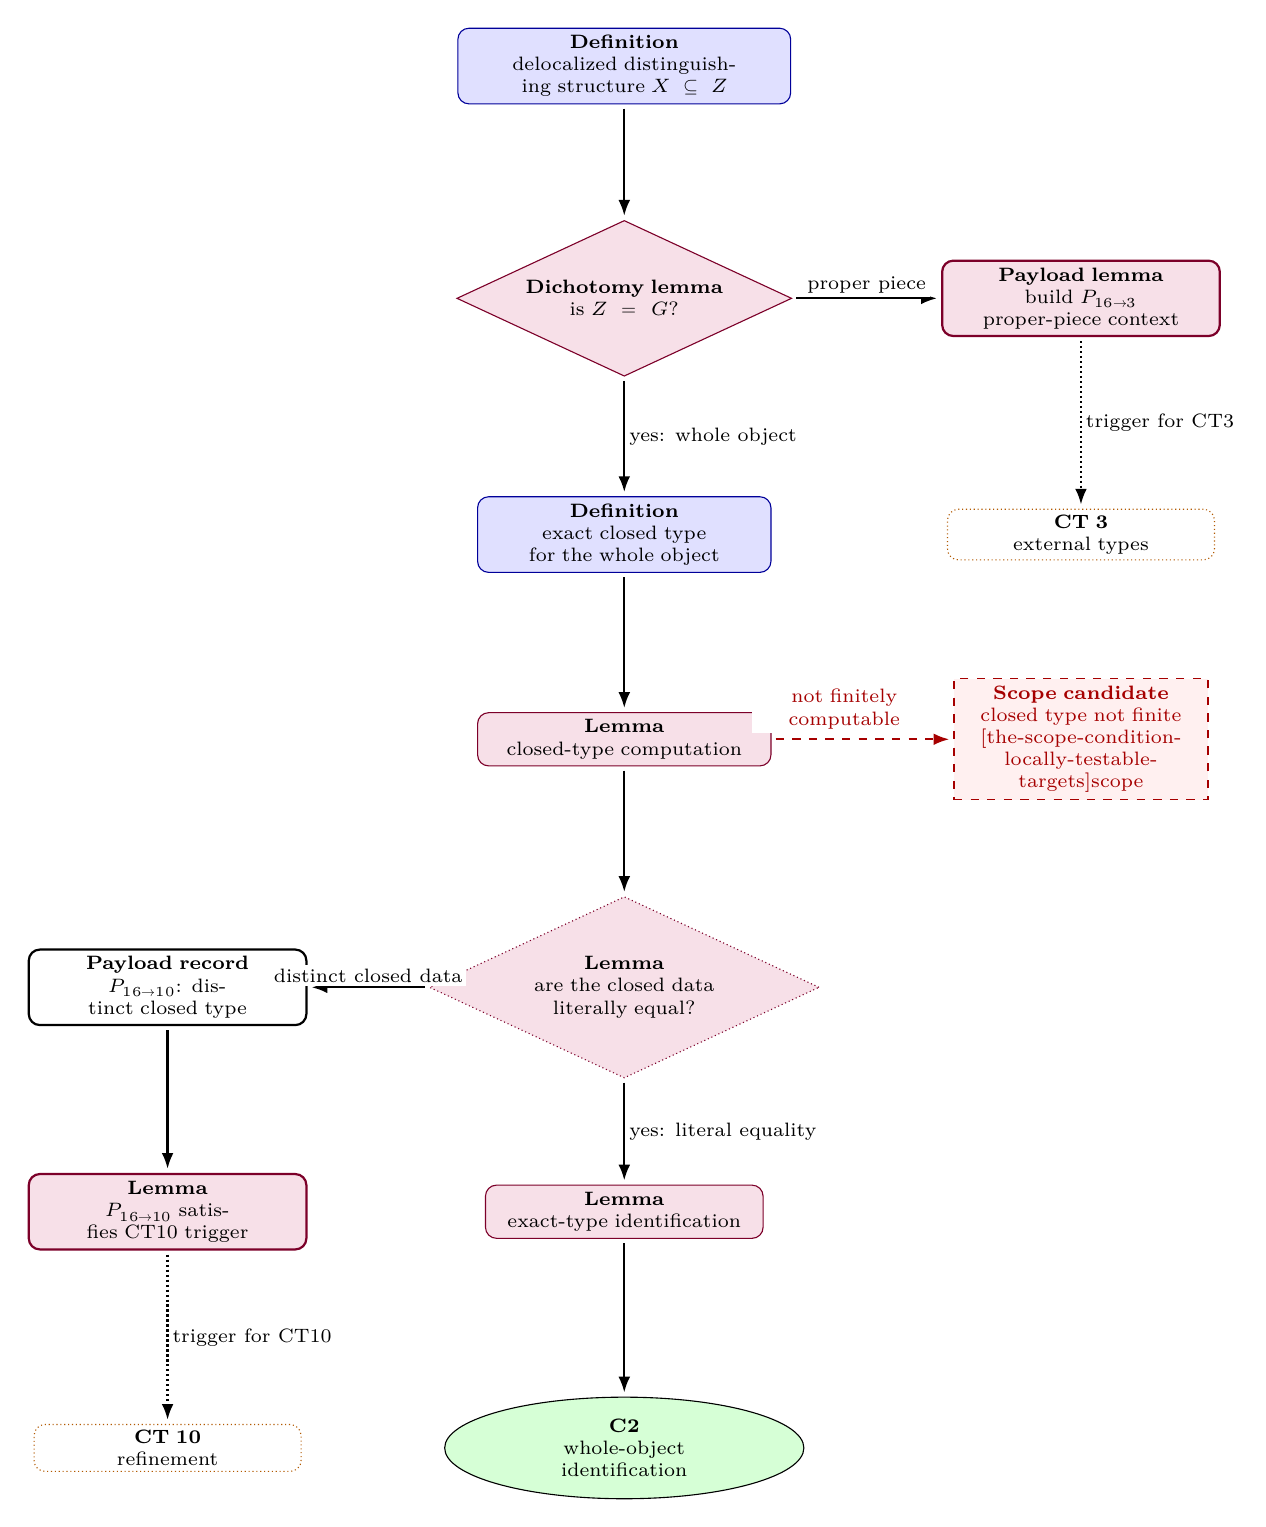
\begin{tikzpicture}[
every node/.style={font=\scriptsize}
]
\node[bcwide,bcdefinition] (input) at (0,0) {\textbf{Definition}\\delocalized distinguishing structure \(X\subseteq Z\)};
\node[bcdec,bclemma,text width=3.05cm,minimum width=3.85cm] (whole) at (0,-2.95) {\textbf{Dichotomy lemma}\\is \(Z=G\)?};
\node[bcbox,bclemma,bcpayload,text width=3.35cm,minimum width=3.35cm] (proper) at (5.80,-2.95) {\textbf{Payload lemma}\\build \(P_{16\to3}\)\\proper-piece context};
\node[bcroute,bcrouteneutral,bcoutputroute,text width=3.25cm,minimum width=3.25cm] (replace) at (5.80,-5.95) {\textbf{CT 3}\\external types};
\node[bcbox,bcdefinition,text width=3.55cm,minimum width=3.55cm] (closedtype) at (0,-5.95) {\textbf{Definition}\\exact closed type for the whole object};
\node[bcbox,bclemma,text width=3.55cm,minimum width=3.55cm] (compute) at (0,-8.55) {\textbf{Lemma}\\closed-type computation};
\node[bcscopefail,text width=3.05cm,minimum width=3.05cm] (scopebad) at (5.80,-8.55) {\textbf{Scope candidate}\\closed type not finite\\\scoperef};
\node[bcdec,bclemma,bccheck,text width=3.05cm,minimum width=3.85cm] (equal) at (0,-11.70) {\textbf{Lemma}\\are the closed data literally equal?};
\node[bcbox,bcpayload,text width=3.35cm,minimum width=3.35cm] (distinct) at (-5.80,-11.70) {\textbf{Payload record}\\\(P_{16\to10}\): distinct closed type};
\node[bcbox,bclemma,bcpayload,text width=3.35cm,minimum width=3.35cm] (defaultlemma) at (-5.80,-14.55) {\textbf{Lemma}\\\(P_{16\to10}\) satisfies CT10 trigger};
\node[bcroute,bcrouteneutral,bcoutputroute,text width=3.25cm,minimum width=3.25cm] (defaultroute) at (-5.80,-17.55) {\textbf{CT 10}\\refinement};
\node[bcbox,bclemma,text width=3.35cm,minimum width=3.35cm] (idlemma) at (0,-14.55) {\textbf{Lemma}\\exact-type identification};
\node[bcclosed,text width=3.05cm,minimum width=3.05cm] (out) at (0,-17.55) {\textbf{C2}\\whole-object identification};
\draw[bcarr] (input)--(whole);
\draw[bcarr] (whole)--node[bclabel,above]{proper piece}(proper);
\draw[bchandoff] (proper)--node[bclabel,right]{trigger for CT3}(replace);
\draw[bcarr] (whole)--node[bclabel,right]{yes: whole object}(closedtype);
\draw[bcarr] (closedtype)--(compute);
\draw[bcscopearr] (compute)--node[bclabel,above,pos=.40,yshift=2pt,text width=2.25cm,align=center]{not finitely computable}(scopebad);
\draw[bcarr] (compute)--(equal);
\draw[bcarr] (equal)--node[bclabel,above]{distinct closed data}(distinct);
\draw[bcarr] (distinct)--(defaultlemma);
\draw[bchandoff] (defaultlemma)--node[bclabel,right]{trigger for CT10}(defaultroute);
\draw[bcarr] (equal)--node[bclabel,right]{yes: literal equality}(idlemma);
\draw[bcarr] (idlemma)--(out);
\end{tikzpicture}%
}
\caption[Closure-tactic 16: whole-object exact types]{Closure-tactic 16 (whole-object exact types).  The tactic is certified by a delocalized-structure definition, a proper-versus-whole dichotomy lemma constructing \(P_{16\to3}\), an exact closed-type definition, a computation lemma, and a literal-equality lemma that either identifies the whole object or routes distinct closed data as \(P_{16\to10}\).  The tactic demands literal closed-type equality; a closed type that is not finitely computable is a candidate scope obstruction referred to the global audit in \secref{the-scope-condition-locally-testable-targets}.  Line grammar (Fig.~\ref{fig:line-grammar-legend}): solid --- intended execution through the construction of the intended residual; dotted --- checks and the post-residual handoff to the consumer tactic; dashed --- design-failure recovery; red-dashed --- candidate scope obstruction referred to the global audit.}
\label{fig:ct16-whole-object-types}
\end{figure}
\FloatBarrier

\subsection*{Whole-object exact types in practice}

When delocalization reaches \(Z=G\), the outside-context class contains
only the empty completion. Outside-extension comparisons therefore
provide no nontrivial distinguishing contexts. CT16 records a separate
\textbf{exact closed type}, computed as an explicit finite data structure,
and permits identification only when those closed types are literally
equal. The certificate is
the closed-form computation itself, together with a lemma stating that
the degenerate empty context induces no additional identifications. An
argument at \(Z=G\) must exhibit the closed type explicitly; equality on
an empty context supplies no equivalence beyond the recorded closed
data.

The low-level diagram for CT16 is Fig.~\ref{fig:ct16-whole-object-types};
it separates the proper-piece route, the whole-object closed-type
computation, literal equality closure, and default-refinement exit.



\subsection{CT17 --- Target thickening}\label{ct:17}\label{target-thickening-bounded-offsets-against-sparse-targets}
\ctsignature{\(\begin{array}{@{}l@{}}
P_{1\to17}\to \ctcert{C1,C5};\\
\ctint{P_{17\to8},P_{17\to14}};\\
\ctrec{P_{17\to3},P_{17\to10}}.
\end{array}\)}

You reach CT17 when CT1's target-avoiding state carries a sparse target
set and a bounded family of offsets.  The tactic thickens sparse target
values inside one branch state and routes the survivors.

\ctpar{Fires when}
The state records a sparse target set \(S\), bounded offsets \(\Delta\),
compatible completion classes \(\Omega\), and target arithmetic data.

\ctpar{You supply}
You supply the offset set, the compatibility classes, the survivor list,
and the arithmetic threshold.

\ctpar{Execution}
Build the offset family inside the current branch state, prove a
compatibility lemma for the completions, enumerate surviving translates
at small scales, and state the orbit or order criterion at
large scales with its threshold solved explicitly.  Each survivor remains
typed by its completion class.

\ctpar{Soundness obligations}
\begin{itemize}
\tightlist
\item \textbf{definition} is instantiated with the sparse target set \(S\), the bounded offset family \(\Delta\), the completion classes \(\Omega\), and the target arithmetic data.
\item \textbf{dichotomy} is instantiated with the finite-range branch and the repeated-increment branch of the scale split.
\item \textbf{composition} is instantiated with the finite survivor enumeration or the large-scale arithmetic comparison.
\item \textbf{routing} is instantiated with \(P_{17\to3}\), \(P_{17\to10}\), \(P_{17\to8}\), and \(P_{17\to14}\) for type separation, label separation, finite survivor sequences, and residual mass.
\item \textbf{trigger} is instantiated with the CT3, CT10, CT8, and CT14 triggers for those target-thickening outputs.
\end{itemize}

\ctpar{Routing}
A target block hit closes by C1; finite survivor exhaustion closes by
C5.  Completion classes route to
CT3 or CT10, finite survivor sequences to CT8, and residual mass to CT14.

\ctpar{Limit}
CT17 is inapplicable when no bounded offset family with arithmetic leverage
is available. The execution error is pooling incompatible offsets without a
class record; the audit records CT17/definition.

\begin{figure}[p]
\centering
\vspace*{-2.80cm}
\resizebox{0.98\textwidth}{!}{%
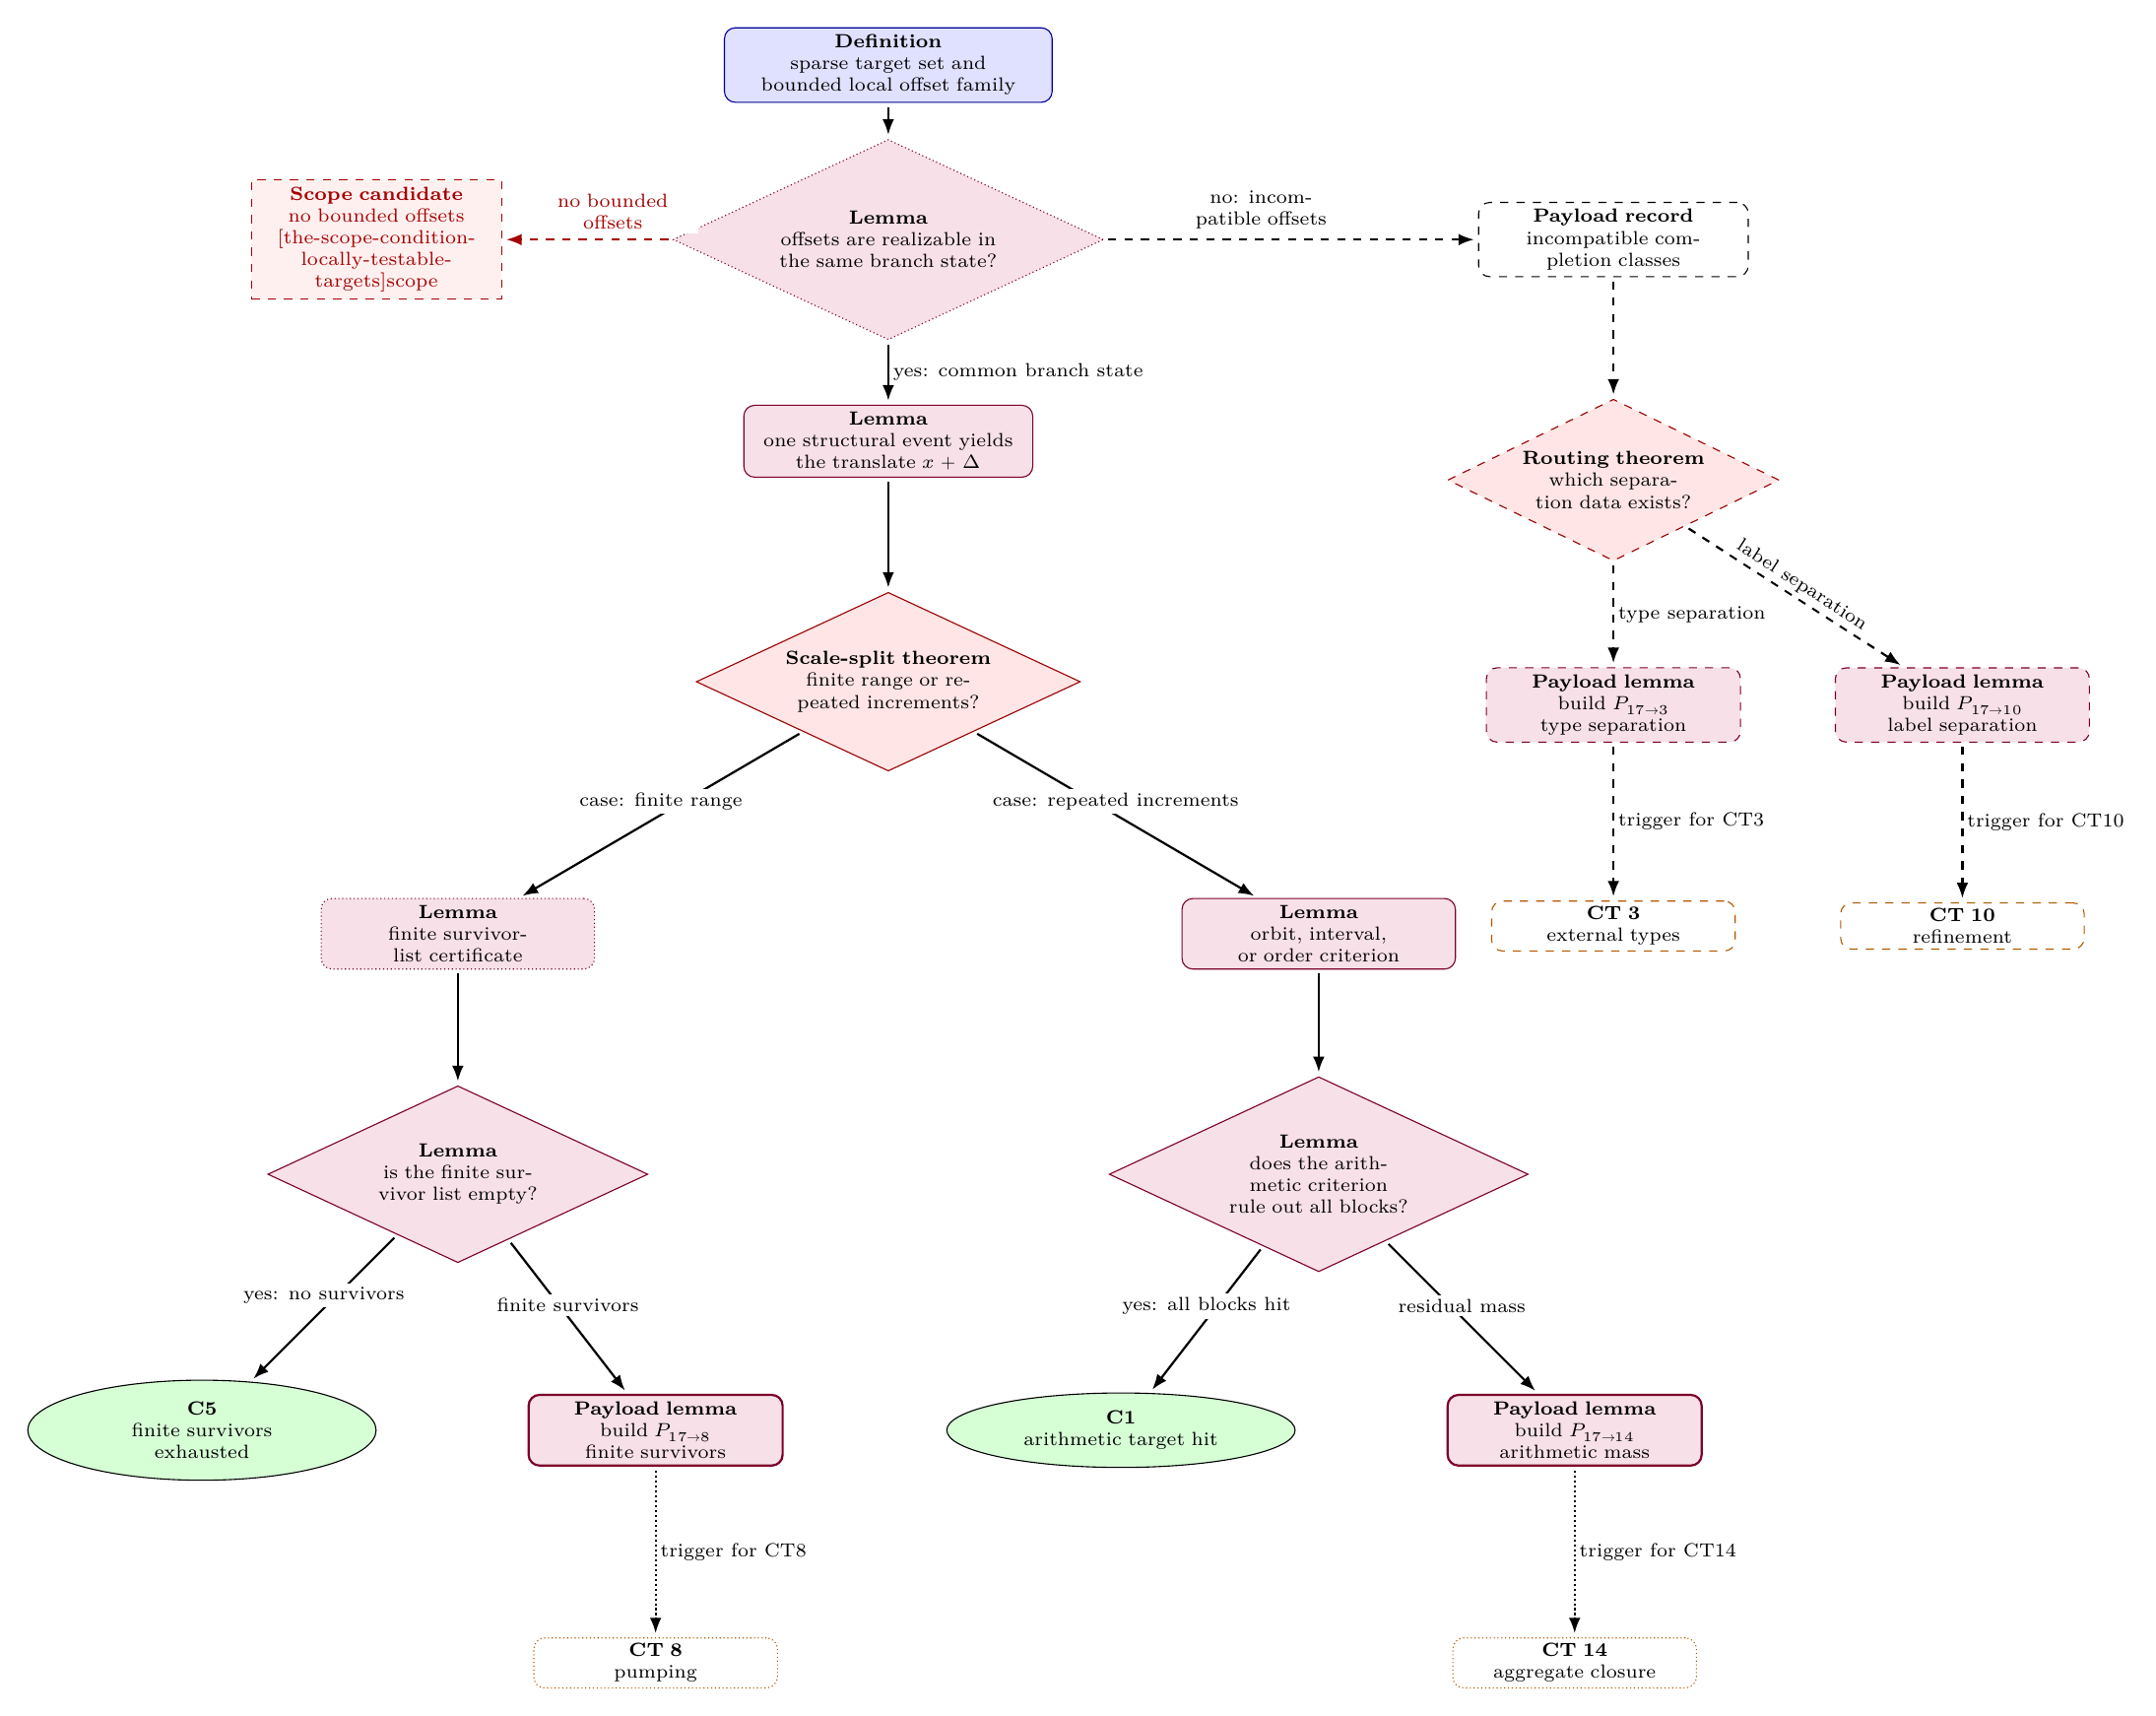
\begin{tikzpicture}[
every node/.style={font=\scriptsize}
]
\node[bcwide,bcdefinition] (input) at (0,0) {\textbf{Definition}\\sparse target set and bounded local offset family};
\node[bcauditbox,text width=3.75cm,minimum width=3.75cm] (compatible) at (0,-2.25) {\textbf{Lemma}\\offsets are realizable in the same branch state?};
\node[bcscopefail,text width=3.05cm,minimum width=3.05cm] (scopebad) at (-6.60,-2.25) {\textbf{Scope candidate}\\no bounded offsets\\\scoperef};
\node[bcbox,bclemma,text width=3.55cm,minimum width=3.55cm] (block) at (0,-4.85) {\textbf{Lemma}\\one structural event yields the translate \(x+\Delta\)};
\node[bcbox,bcdesign,text width=3.30cm,minimum width=3.30cm] (compres) at (9.35,-2.25) {\textbf{Payload record}\\incompatible completion classes};
\node[bcdec,bctheorem,text width=3.05cm,minimum width=3.85cm] (scale) at (0,-7.95) {\textbf{Scale-split theorem}\\finite range or repeated increments?};
\node[bcroutechoice,bctheorem,bcdesign,text width=2.55cm,minimum width=3.15cm] (compchoice) at (9.35,-5.35) {\textbf{Routing theorem}\\which separation data exists?};
\node[bcbox,bclemma,bcdesign,text width=3.10cm,minimum width=3.10cm] (typelemma) at (9.35,-8.25) {\textbf{Payload lemma}\\build \(P_{17\to3}\)\\type separation};
\node[bcbox,bclemma,bcdesign,text width=3.10cm,minimum width=3.10cm] (labellemma) at (13.85,-8.25) {\textbf{Payload lemma}\\build \(P_{17\to10}\)\\label separation};
\node[bcbox,bclemma,bccheck,text width=3.35cm,minimum width=3.35cm] (finite) at (-5.55,-11.20) {\textbf{Lemma}\\finite survivor-list certificate};
\node[bcroute,bcrouteneutral,bcdesign,text width=3.00cm,minimum width=3.00cm] (typeroute) at (9.35,-11.10) {\textbf{CT 3}\\external types};
\node[bcroute,bcrouteneutral,bcdesign,text width=3.00cm,minimum width=3.00cm] (labelroute) at (13.85,-11.10) {\textbf{CT 10}\\refinement};
\node[bcdec,bclemma,text width=3.00cm,minimum width=3.75cm] (empty) at (-5.55,-14.30) {\textbf{Lemma}\\is the finite survivor list empty?};
\node[bcclosed,text width=3.00cm,minimum width=3.00cm] (targetclose) at (-8.85,-17.60) {\textbf{C5}\\finite survivors exhausted};
\node[bcbox,bclemma,bcpayload,text width=3.10cm,minimum width=3.10cm] (finitelemma) at (-3.00,-17.60) {\textbf{Payload lemma}\\build \(P_{17\to8}\)\\finite survivors};
\node[bcroute,bcrouteneutral,bcoutputroute,text width=3.00cm,minimum width=3.00cm] (finitefig) at (-3.00,-20.60) {\textbf{CT 8}\\pumping};
\node[bcbox,bclemma,text width=3.35cm,minimum width=3.35cm] (orbit) at (5.55,-11.20) {\textbf{Lemma}\\orbit, interval, or order criterion};
\node[bcdec,bclemma,text width=3.00cm,minimum width=3.75cm] (arithq) at (5.55,-14.30) {\textbf{Lemma}\\does the arithmetic criterion rule out all blocks?};
\node[bcclosed,text width=3.00cm,minimum width=3.00cm] (arithclose) at (3.00,-17.60) {\textbf{C1}\\arithmetic target hit};
\node[bcbox,bclemma,bcpayload,text width=3.10cm,minimum width=3.10cm] (masslemma) at (8.85,-17.60) {\textbf{Payload lemma}\\build \(P_{17\to14}\)\\arithmetic mass};
\node[bcroute,bcrouteneutral,bcoutputroute,text width=3.00cm,minimum width=3.00cm] (arith) at (8.85,-20.60) {\textbf{CT 14}\\aggregate closure};
\draw[bcarr] (input)--(compatible);
\draw[bcscopearr] (compatible)--node[bclabel,above,pos=.35,yshift=2pt,text width=2.10cm,align=center]{no bounded offsets}(scopebad);
\draw[bcrecoverarr] (compatible)--node[bclabel,above,pos=.42,yshift=2pt,text width=2.30cm,align=center]{no: incompatible offsets}(compres);
\draw[bcrecoverarr] (compres)--(compchoice);
\draw[bcrecoverarr] (compchoice)--node[bclabel,right]{type separation}(typelemma);
\draw[bcrecoverarr] (compchoice)--node[bclabel,above,sloped]{label separation}(labellemma);
\draw[bcrecoverarr] (typelemma)--node[bclabel,right]{trigger for CT3}(typeroute);
\draw[bcrecoverarr] (labellemma)--node[bclabel,right]{trigger for CT10}(labelroute);
\draw[bcarr] (compatible)--node[bclabel,right]{yes: common branch state}(block);
\draw[bcarr] (block)--(scale);
\draw[bcarr] (scale)--node[bclabel,above]{case: finite range}(finite);
\draw[bcarr] (scale)--node[bclabel,above]{case: repeated increments}(orbit);
\draw[bcarr] (finite)--(empty);
\draw[bcarr] (empty)--node[bclabel,above]{yes: no survivors}(targetclose);
\draw[bcarr] (empty)--node[bclabel,above]{finite survivors}(finitelemma);
\draw[bchandoff] (finitelemma)--node[bclabel,right]{trigger for CT8}(finitefig);
\draw[bcarr] (orbit)--(arithq);
\draw[bcarr] (arithq)--node[bclabel,above]{yes: all blocks hit}(arithclose);
\draw[bcarr] (arithq)--node[bclabel,above]{residual mass}(masslemma);
\draw[bchandoff] (masslemma)--node[bclabel,right]{trigger for CT14}(arith);
\end{tikzpicture}%
}
\caption[Closure-tactic 17: target thickening]{Closure-tactic 17 (target thickening).  The tactic is certified by target and offset definitions, a compatibility lemma, a thickening lemma, a scale-split theorem, a finite survivor-list certificate, and an arithmetic criterion.  Its terminal exits are C5 when the finite survivor list is exhausted and C1 when the large-scale arithmetic criterion forces a target hit.  Otherwise it constructs \(P_{17\to8}\) for finite-state pumping or \(P_{17\to14}\) for downstream aggregate closure; named incompatible completion classes construct \(P_{17\to3}\) or \(P_{17\to10}\).  Absence of a bounded offset family with arithmetic leverage is a candidate scope obstruction referred to the global audit in \secref{the-scope-condition-locally-testable-targets}.  Line grammar (Fig.~\ref{fig:line-grammar-legend}): solid --- intended execution through the construction of the intended residual; dotted --- checks and the post-residual handoff to the consumer tactic; dashed --- design-failure recovery; red-dashed --- candidate scope obstruction referred to the global audit.}
\label{fig:ct17-target-thickening}
\end{figure}
\FloatBarrier

\subsection*{Target thickening in practice}

When the target lengths or values form a sparse set (powers, primes, a
lacunary sequence), \textbf{target thickening} supplies the arithmetic
leverage. This is the local branch-state analogue of the broader
cycle-length forcing background around even cycles and sparse cycle
lengths
\citep{bondy-simonovits-1974-even-cycles, sudakov-verstraete-2008-cycle-lengths}.
Identify a bounded family of local offsets, i.e.~shifts realizable
inside a single bounded piece. For a base value \(x\), define its
\emph{offset block} by
\(x+\Delta=\{x+d:d\in\Delta\}\). No consecutiveness is assumed unless it
is part of the supplied arithmetic lemma.

Avoidance of the sparse target becomes avoidance of thickened blocks,
which is a strong arithmetic constraint. At small scales, only finitely
many block positions dodge the target, and those positions become finite
label classes. At large scales, repeated bounded increments make the
blocks sweep intervals or residue classes, where orbit and order
arguments apply. The certificate is the explicit finite list of
surviving block positions plus the arithmetic criterion at large scales.
The compatibility audit requires all offsets to be realizable within the
\emph{same} branch state; offsets requiring incompatible completions must
be named and routed rather than pooled into one block.

The low-level diagram for CT17 is Fig.~\ref{fig:ct17-target-thickening};
it records the compatibility audit, block construction, scale split,
finite-survivor route, arithmetic-mass route, and completion-class exits.

\section{The strategy manual}\label{part-iii-the-strategy-manual}

\secref{part-iii-the-strategy-manual} contains policy: the rules for proposing, admitting,
selecting, parameterizing, and composing tactic invocations. It uses the
\secref{part-ii-the-tactic-library} entry data, especially triggers, parameters, cost classes, and
producer/consumer fields, but it does not redefine the internal
procedure of any tactic. General branch design and tactic-choice
discipline live here; CT-local implementation instructions live in the
corresponding entries of \secref{part-ii-the-tactic-library}.

\subsection{Runtime model}\label{runtime-model}

The proof state is a triple
\[
(\text{branch tree},\ \text{payload queue},\ \text{registers}).
\]
The branch tree records the current residuals and closed leaves. The
payload queue contains unconsumed typed messages \(P_{i\to j}\). The
registers are the invariant register, ledger deposits, slack table,
defect register, resilience register, and worksheet list.

The runtime loop is:
\[
\text{state+queue}\to\text{propose}\to\text{admit}\to\text{select}
\to\text{execute}\to\text{route}\to\text{record}.
\]
Three phases are deliberately separated. \textbf{Before} a tactic
invocation, the strategy layer proposes a trigger, checks admission, and
synthesizes parameters. \textbf{Between} invocations, routed payloads are
queued, consumed, or deliberately composed. \textbf{Alongside}
invocations, worksheets and registers are written. Nothing strategic
enters \textbf{during} a tactic: once an admitted CT\(k\)-\(\#\)
invocation starts, execution is the mechanism of \secref{part-ii-the-tactic-library}.

\begingroup
\small
\setlength{\tabcolsep}{2pt}
\begin{longtable}[]{@{}
  >{\raggedright\arraybackslash}p{0.24\linewidth}
  >{\raggedright\arraybackslash}p{0.16\linewidth}
  >{\raggedright\arraybackslash}p{0.52\linewidth}@{}}
\toprule\noalign{}
Pattern & Phase & Role \\
\midrule\noalign{}
\endhead
\bottomrule\noalign{}
\endlastfoot
Both-sides test & before & Admission criterion for a proposed invariant or trigger. \\
Bookkeeping-vs-theorem test & before & Rejects a proposed step that imports a new global theorem instead of spending local resources. \\
Invariant ladder & before & Orders branch predicates so later estimates never assume an unproved normalization. \\
Parameter synthesis (\secref{parameter-synthesis}) & before & Manufactures labels, generators, ledgers, budgets, rates, and measures. \\
Typed payload graph & between & Forced routing of emitted residual payloads to consumer triggers. \\
Sequencing and spines & between & Deliberate composition of admitted invocations, with S-Meas on cycles. \\
Black-box isolation & between & Imports external theorems through declared interfaces. \\
Certificates C1--C5 & halt & Terminal success returns. \\
Checklists, worksheets, registers & alongside & Verification artifacts that audit both mechanism and policy. \\
Resilience and defect registers & alongside & Failure semantics and repair history. \\
\end{longtable}
\endgroup

The queue discipline is strict: consume a queued payload before
synthesizing a fresh one unless the selection policy below records a
reason to defer it. This prevents the proof from accumulating orphan
residuals whose routing is no longer visible.  The queue may be empty
only when the branch is closed or the active tactic is operating
directly on the current residual condition.

Figure~\ref{fig:strategy-runtime-loop} displays the runtime workflow.
In every strategy figure below, yellow nodes mark genuine policy choices,
dotted diamonds mark checks whose outcome is determined by recorded data,
solid arrows mark ordinary execution, dotted arrows mark typed or artifact
handoffs, and dashed arrows mark repair or re-entry.

\begin{figure}[htbp]
\centering
\resizebox{0.98\textwidth}{!}{%
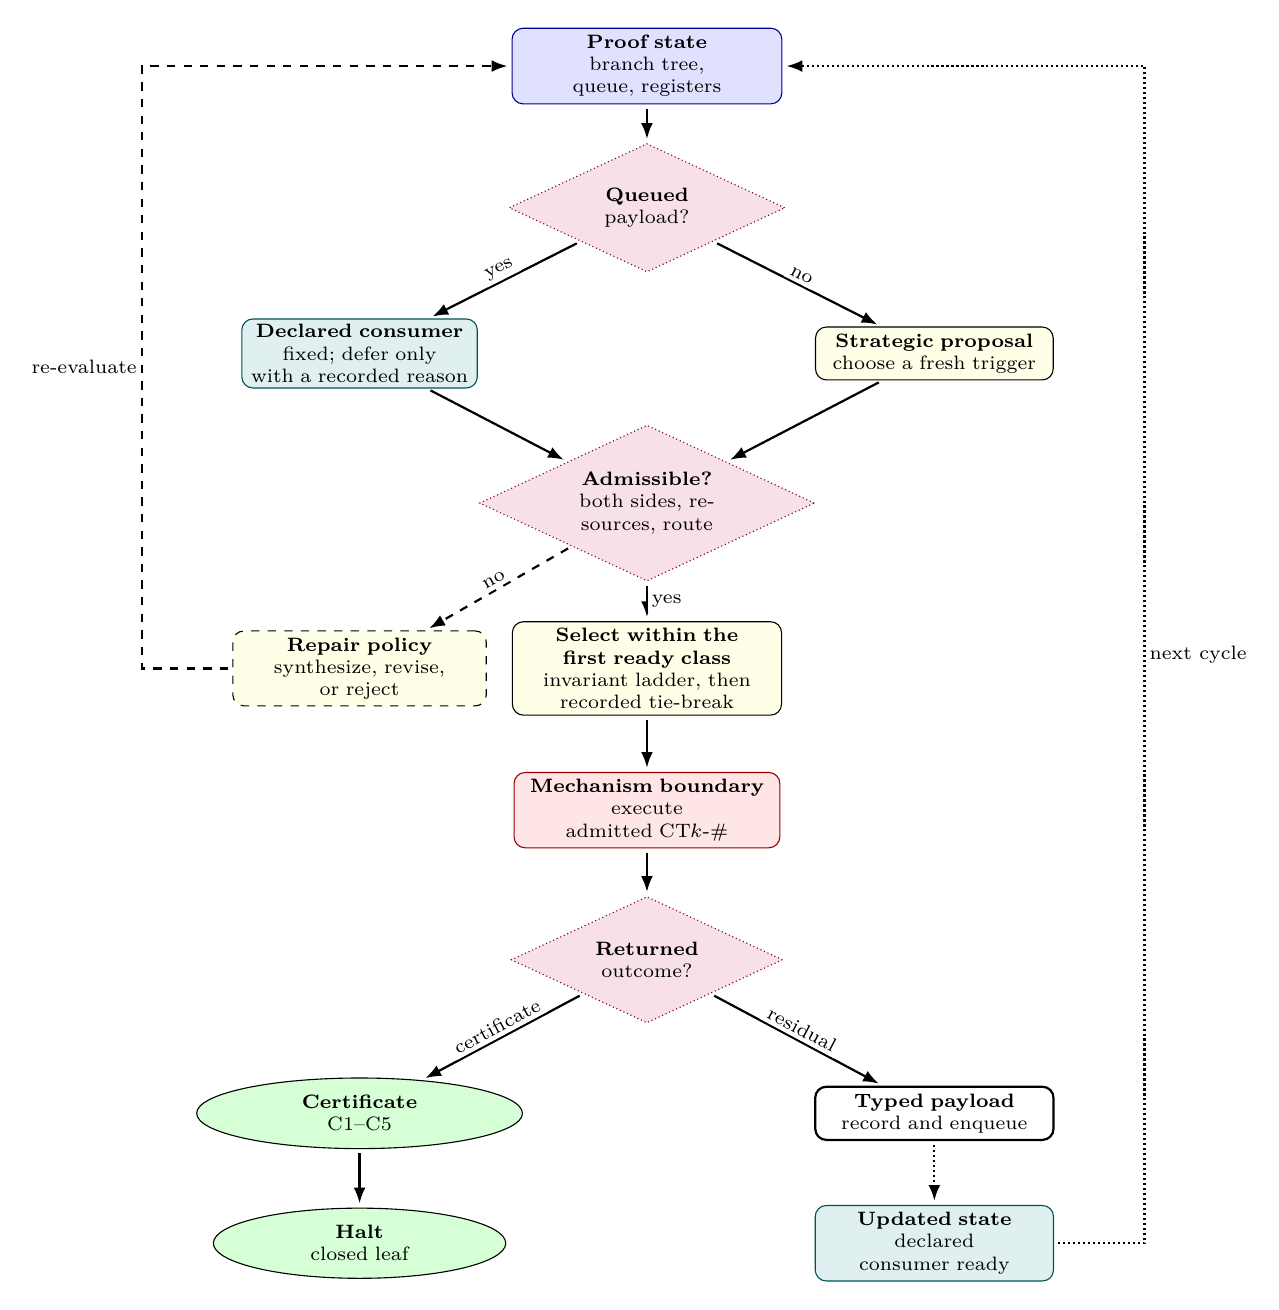
\begin{tikzpicture}[
x=1cm,
y=1cm,
every node/.style={font=\scriptsize}
]
\node[bcwide,bcdefinition,text width=3.25cm,minimum width=3.25cm]
  (state) at (0,0) {\textbf{Proof state}\\branch tree, queue, registers};
\node[bcdec,bcaudit,text width=2.20cm,minimum width=2.95cm]
  (queued) at (0,-1.80) {\textbf{Queued}\\payload?};
\node[bcroute,bccorollary,text width=2.85cm,minimum width=2.85cm]
  (forced) at (-3.65,-3.65) {\textbf{Declared consumer}\\fixed; defer only\\with a recorded reason};
\node[bcroutepanel,text width=2.85cm,minimum width=2.85cm]
  (fresh) at (3.65,-3.65) {\textbf{Strategic proposal}\\choose a fresh trigger};
\node[bcdec,bcaudit,text width=2.35cm,minimum width=3.10cm]
  (admit) at (0,-5.55) {\textbf{Admissible?}\\both sides, resources, route};
\node[bcroutepanel,text width=3.25cm,minimum width=3.25cm]
  (select) at (0,-7.65) {\textbf{Select within the first ready class}\\invariant ladder, then recorded tie-break};
\node[bcbox,bctheorem,text width=3.20cm,minimum width=3.20cm]
  (execute) at (0,-9.45) {\textbf{Mechanism boundary}\\execute\\admitted CT\(k\)-\(\#\)};
\node[bcdec,bcaudit,text width=2.25cm,minimum width=3.00cm]
  (outcome) at (0,-11.35) {\textbf{Returned}\\outcome?};
\node[bcclosed,text width=2.75cm,minimum width=2.75cm]
  (certificate) at (-3.65,-13.30) {\textbf{Certificate}\\C1--C5};
\node[bcbox,bcpayload,text width=2.85cm,minimum width=2.85cm]
  (payload) at (3.65,-13.30) {\textbf{Typed payload}\\record and enqueue};
\node[bcclosed,text width=2.45cm,minimum width=2.45cm]
  (halt) at (-3.65,-14.95) {\textbf{Halt}\\closed leaf};
\node[bcbox,bccorollary,text width=2.85cm,minimum width=2.85cm]
  (updated) at (3.65,-14.95) {\textbf{Updated state}\\declared\\consumer ready};
\node[bcroutepanel,bcdesign,text width=3.05cm,minimum width=3.05cm]
  (repair) at (-3.65,-7.65) {\textbf{Repair policy}\\synthesize, revise,\\or reject};
\draw[bcarr] (state)--(queued);
\draw[bcarr] (queued)--node[bclabel,above,sloped]{yes}(forced);
\draw[bcarr] (queued)--node[bclabel,above,sloped]{no}(fresh);
\draw[bcarr] (forced)--(admit);
\draw[bcarr] (fresh)--(admit);
\draw[bcarr] (admit)--node[bclabel,right]{yes}(select);
\draw[bcrecoverarr] (admit)--node[bclabel,above,sloped]{no}(repair);
\draw[bcarr] (select)--(execute);
\draw[bcarr] (execute)--(outcome);
\draw[bcarr] (outcome)--node[bclabel,above,sloped]{certificate}(certificate);
\draw[bcarr] (outcome)--node[bclabel,above,sloped]{residual}(payload);
\draw[bcarr] (certificate)--(halt);
\draw[bchandoff] (payload)--(updated);
\draw[bchandoff] (updated.east) -- ++(1.15,0) |- node[bclabel,right,pos=0.25]{next cycle} (state.east);
\draw[bcrecoverarr] (repair.west) -- ++(-1.15,0) |- node[bclabel,left,pos=0.25]{re-evaluate} (state.west);
\end{tikzpicture}%
}
\caption[Strategy runtime loop]{Strategy runtime loop.  Queued payloads retain their declared consumers; fresh triggers and recorded tie-breaks are policy choices.  Failed admission returns to repair, and every nonterminal output is requeued as a typed payload.}
\label{fig:strategy-runtime-loop}
\end{figure}

\subsection{Branch states}\label{branch-states}

A branch is created whenever the proof uses a dichotomy: property \(P\)
holds or fails. The branch state records the cumulative context:

\[
\mathfrak B_P = \mathfrak B_{\mathrm{prev}} + P
\qquad\text{or}\qquad
\mathfrak B_{\neg P} = \mathfrak B_{\mathrm{prev}} + \neg P.
\]

The failure branch must be \emph{meaningful}. If \(P\) is an accounting
statement, \(\neg P\) must force an overload (\secref{the-branch-taxonomy}). If \(P\) is a
structural statement, \(\neg P\) must force a residual shape. If \(P\)
is a target hit, \(\neg P\) asserts the absence of all target-hitting
local tests. This is what gives each branch a finite or measurable state
space.

\subsection{Closure criteria and the branch
table}\label{closure-criteria-and-the-branch-table}

\subsubsection{What counts as a finished
branch}\label{what-counts-as-a-finished-branch}

A branch is finished only when every leaf is one of:

\begin{enumerate}
\def\labelenumi{\arabic{enumi}.}
\tightlist
\item \textbf{C1.} a direct target contradiction;
\item \textbf{C2.} a minimality contradiction;
\item \textbf{C3.} an entry in an already-routed defect account;
\item \textbf{C4.} a bounded-capacity contradiction;
\item \textbf{C5.} a finite, verified impossibility.
\end{enumerate}

These five certificates are the fixed closure alphabet for the whole
document. Every branch-level success must name one of C1--C5 and must do
so by a route that the branch table can record.

A branch remains open whenever its final line gives only an informal
plausibility judgment; \appref{appendix-d.-quick-reference-card} records
the canonical prompt-lint examples.

\subsubsection{The branch table}\label{the-branch-table}

Every complete branch closure terminates in a table of the following
form. The table records every residual explicitly.

\begingroup
\scriptsize
\setlength{\tabcolsep}{1.5pt}
\begin{longtable}[]{@{}
  >{\raggedright\arraybackslash}p{(\columnwidth - 10\tabcolsep) * \real{0.1500}}
  >{\raggedright\arraybackslash}p{(\columnwidth - 10\tabcolsep) * \real{0.2350}}
  >{\raggedright\arraybackslash}p{(\columnwidth - 10\tabcolsep) * \real{0.1400}}
  >{\raggedright\arraybackslash}p{(\columnwidth - 10\tabcolsep) * \real{0.1550}}
  >{\raggedright\arraybackslash}p{(\columnwidth - 10\tabcolsep) * \real{0.1500}}
  >{\raggedright\arraybackslash}p{(\columnwidth - 10\tabcolsep) * \real{0.1700}}@{}}
\toprule\noalign{}
\begin{minipage}[b]{\linewidth}\raggedright
Branch
\end{minipage} & \begin{minipage}[b]{\linewidth}\raggedright
Residual condition
\end{minipage} & \begin{minipage}[b]{\linewidth}\raggedright
Demand
\end{minipage} & \begin{minipage}[b]{\linewidth}\raggedright
Payer
\end{minipage} & \begin{minipage}[b]{\linewidth}\raggedright
Bounded multiplicity
\end{minipage} & \begin{minipage}[b]{\linewidth}\raggedright
Closure
\end{minipage} \\
\midrule\noalign{}
\endhead
\bottomrule\noalign{}
\endlastfoot
Direct hit & local test realized & none & none & n/a & contradiction \\
Defect & outside context distinguishes pieces & defective quotient &
defect account & canonical piece & routed \\
Compression & no context distinguishes smaller piece & piece size &
minimality & n/a & contradiction \\
Overload & demands exceed capacity & bad local objects & payer capacity
& matching/\allowbreak star & bounded exchange \\
Dormant / low entropy & local tests absent & first failures &
obstructions/\allowbreak chains & first-failure map & exchange trichotomy \\
Long chain & many bounded states & type sequence & exact types &
pigeonhole & compression/\allowbreak defect \\
Bounded residual & finite local package & finite states & enumeration &
exhaustive table & no leaf survives \\
\end{longtable}
\endgroup



\subsection{Branch taxonomy}\label{the-branch-taxonomy}

A new branch is admissible when the proof possesses a reliable routing
principle for it. Two recurring verbs first: a residual is
\textbf{routed} when it is mapped, by a canonical rule, into a
previously named branch that has its own closure (so membership is the
remaining obligation); and a demand is \textbf{charged} when the
charging scheme assigns it a payer.

The admissible branch types are the following.

\textbf{Direct-hit branch.} A local configuration realizes the target:
\(X \Rightarrow T\). The branch closes immediately.

\textbf{Defect branch.} Two pieces that were supposed to be equivalent
are distinguished by some outside context:

\[
\exists\, C_{\mathrm{out}}:\quad T(X\cup C_{\mathrm{out}}) \ne T(X'\cup C_{\mathrm{out}}).
\]

The piece is then \textbf{target-defective}. A defect enters the
\textbf{defect account} (a designated charging scheme whose demands are
the defective pieces themselves) or a previously named route. A defect
may also be consumed iteratively rather than all at once; see the
peeling loops of \secref{peeling-loops-closure-by-well-founded-recursion}.

\textbf{Compression branch.} Two pieces are indistinguishable against
all outside contexts and one is smaller:

\[
\tau(X') = \tau(X), \qquad |X'| < |X|.
\]

Minimality kills the branch. This move is called a \textbf{compression}.

\textbf{Delocalization branch.} The distinguishing structure spreads
beyond the local \textbf{cell} to a larger piece \(X \subsetneq Z\). A
cell is an inclusion-minimal piece of the decomposition induced by the
current branch state: the smallest unit to which finite labels are
attached.

If \(Z\) is proper, replacement/minimality applies. If \(Z = G\), a
global type or \textbf{barrier argument} must be invoked explicitly. A
barrier argument shows that a separating structure in \(G\) controls all
target tests crossing it, so that the global external type itself
excludes the target. Any such invocation must be audited as a global
step in the sense of \secref{bookkeeping-versus-new-theorems}. The \(Z=G\) case requires special care
because its context is degenerate; see \secref{the-whole-object-piece-exact-types-under-context-degeneracy}.

\textbf{Overload branch.} A demand count exceeds a payer capacity:
\(|\mathcal D| > C|\mathcal P|\). This situation is an
\textbf{overload}. High load creates a homogeneous substructure via
pigeonhole or matching/star extraction.

\textbf{Monochromatic-family branch.} Each demand carries a finite
\textbf{label} describing its combinatorial role in the charging scheme.
When a charging scheme is overloaded, pigeonhole over the finitely many
labels extracts a large \textbf{monochromatic subfamily} --- a subfamily
of demands all bearing the same label:

\[
\mathcal D_\lambda = \{d \in \mathcal D : \operatorname{label}(d) = \lambda\}.
\]

If \(|\mathcal D_\lambda|\) is large, extraction inside a single label
class produces a matching, a star, a long \textbf{chain}, a repeated
external type, or a bounded family of \textbf{local exchanges}. A chain
is a maximal sequence of bounded-width pieces glued consecutively along
their boundaries, i.e.~a long path of cells.

A local exchange is a bounded local operation, presented as two
representatives with the same interface, that changes a target-relevant
quantity by a bounded increment; its full analysis is the exchange
trichotomy of \secref{the-exchange-trichotomy}. Each extracted structure is routed by direct
hit, defect, compression, \textbf{auxiliary routing} (delegation to a
designated side branch maintained for this purpose), or finite
exhaustion.

\textbf{Terminal-residual branch.} A branch becomes terminal after every
other exit has been formally excluded, where an \textbf{exit} is any of
the named closure routes above. Terminal residuals are finite, bounded,
or equipped with a strict global deficit that the available charging
schemes cannot carry. A terminal residual carries exact data:

\[
\begin{aligned}
\text{terminal residual}
={}&
\text{local piece}
+
\text{branch state}\\
&+
\text{absence of exits}
+
\text{minimality / carrier / type data}.
\end{aligned}
\]

The exactness requirement is load-bearing: the recorded data is
frequently what kills the terminal residual, because the data a residual
is forced to carry can contradict the exit absences that define it.



\subsection{The general branch-closure
algorithm}\label{the-general-branch-closure-algorithm}

Three remaining terms are used below. The \textbf{local degrees of
freedom} of a piece are the independent bounded modifications available
at it; few degrees of freedom mean rigidity, hence structure. A local
exchange is \textbf{neutral} if no compatible outside context
distinguishes its two representatives (\secref{the-exchange-trichotomy}). A \textbf{carrier
quotient} identifies pieces that share the same carrier data, collapsing
the state space to finitely many classes. A \textbf{charge transfer}
canonically relocates a demand from a saturated or ineligible payer to a
designated high-degree neighbour, exactly as in a discharging rule
\citep{cranston-west-2017-discharging}.

\begin{algorithm}[General branch-closure procedure]\label{alg:general-branch-closure}
\leavevmode
\begin{description}
\item[Input.] A minimal counterexample \(G\), a target predicate \(T\)
with its local-test family, and a branch state \(\mathfrak B\).
\item[Output.] Either a closed branch, or a named residual with exact
data that is smaller, finite, charged, or routed.
\end{description}

\begin{enumerate}
\def\labelenumi{\arabic{enumi}.}
\tightlist
\item
Define the local state space: list the bounded objects visible in
\(\mathfrak B\) (windows, cells, chains, payers, exchanges, and
carriers) and assign finite labels to their local configurations.
\item
State the branch dichotomy: either a local test is live, the local
structure is rich, or the relevant capacity comparison closes; otherwise
the failed alternative creates a recorded residual condition.
\item
On a target-rich branch, close by the available counting, entropy,
density, or direct target-realization argument.
\item
On a target-poor branch, convert target-poorness into recorded
structure: few local degrees of freedom, a repeated external type, a
bounded chain, a neutral exchange, a carrier quotient, a charge
transfer, or a routed residual.
\item
Charge the recorded structure: define the demands, assign canonical
payers, and prove the required bounded-multiplicity statement.
\item
When a payer is overloaded, extract a labelled homogeneous subfamily and
route the resulting matching, star, chain, or exchange by finite case
analysis.
\item
When a labelled state repeats, compare exact external types: a repetition
visible to some context gives a target defect, while a repetition
invisible to every context gives compression.
\item
When the remaining state space is finite, enumerate it.  Every leaf must
be a target hit, a defect, a compression, a delocalization, an auxiliary
branch, or a charging contradiction.
\item
Update the branch table: every failure route becomes a named branch and
every residual receives a typed name.
\end{enumerate}
\end{algorithm}

In Step 5, a \textbf{local obstruction} is a bounded structure that
explains why a local test fails to fire at a given site.  It is a
candidate payer only after a canonical assignment and a
bounded-multiplicity or capacity estimate have been proved.

The algorithm is a design discipline. A step closes a branch when it
produces a closed leaf or a residual that is smaller, finite, charged,
or routed.

\subsection{Admission}\label{admission}

A proposed tactic invocation enters the queue only after two admission
tests.

\textbf{Both-sides test.} A proposed branch predicate or invariant must
fill four blanks:
\[
\begin{array}{ll}
\text{positive side:} & \text{what does it pay, and into which account?}\\
\text{negative side:} & \text{what bounded residual does it force?}\\
\text{measurability:} & \text{is the predicate recorded in }\mathfrak B?\\
\text{route:} & \text{which CT trigger receives the residual payload?}
\end{array}
\]
If any blank is empty, the proposal is not an admitted trigger; it is a
parameter-synthesis task or a defect-register item.

\textbf{Bookkeeping-vs-theorem test.} A proposed step is admitted as a
library instantiation only when it spends existing local resources:
finite labels, bounded interfaces, local exchanges, ledgers, or
recorded budgets. If the step requires an unconditional theorem about
all large objects with a global property, it is not a tactic invocation.
It must be replaced by a first failure, finite state, compression,
black-box input, or an explicit level-3 pattern addition.

Figure~\ref{fig:strategy-admission-gates} displays the two admission
gates.

\begin{figure}[htbp]
\centering
\resizebox{0.98\textwidth}{!}{%
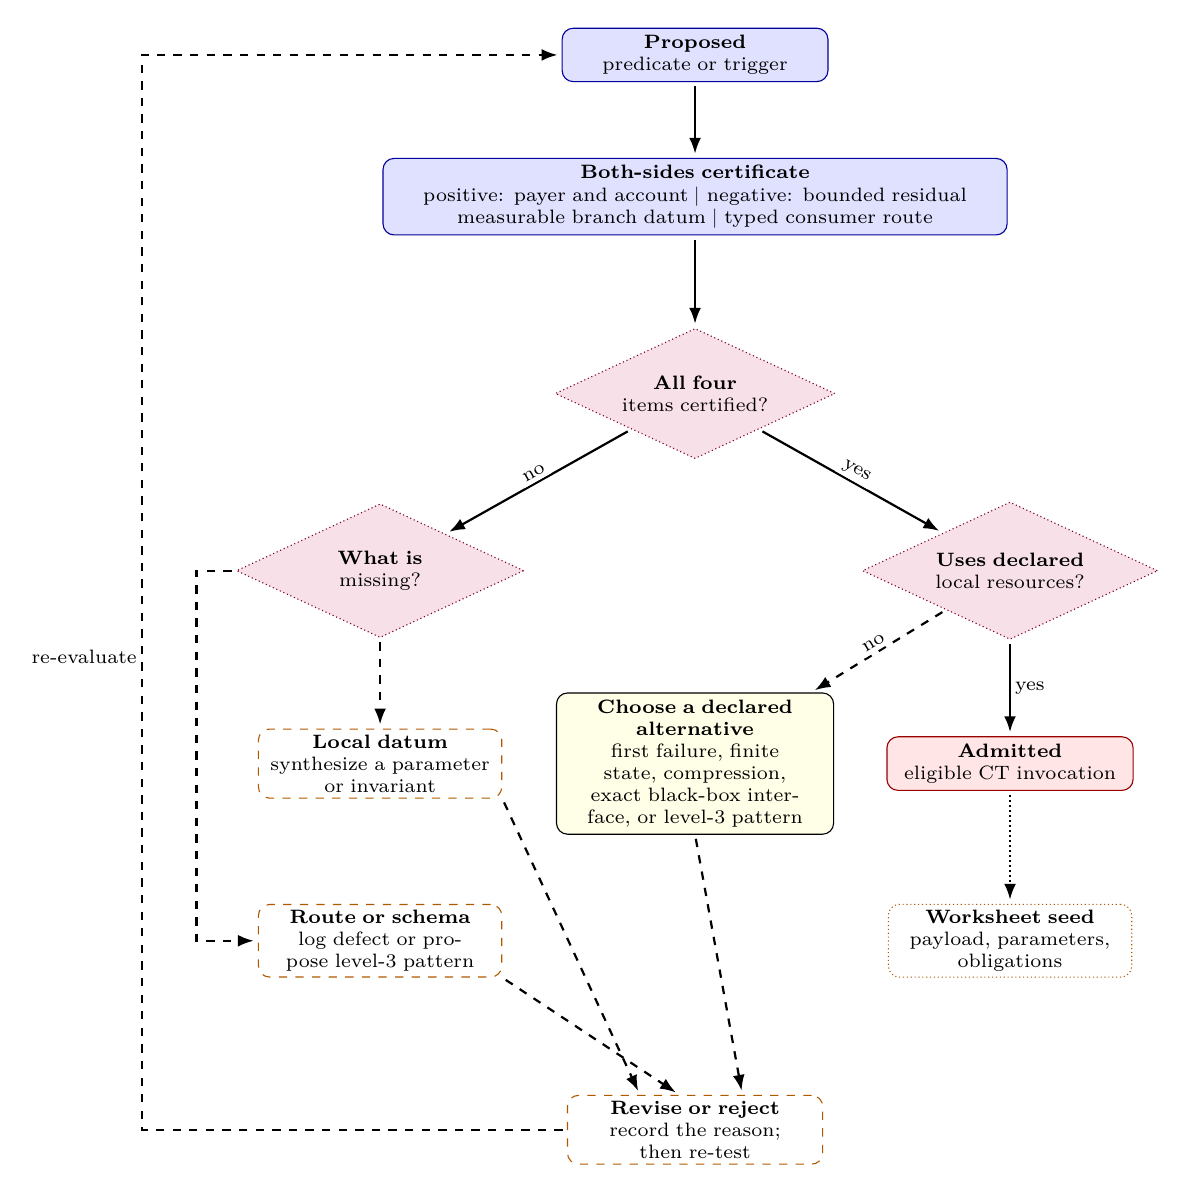
\begin{tikzpicture}[
x=1cm,
y=1cm,
every node/.style={font=\scriptsize}
]
\node[bcwide,bcdefinition,text width=3.20cm,minimum width=3.20cm]
  (proposal) at (0,0) {\textbf{Proposed}\\predicate or trigger};
\node[bcwide,bcdefinition,text width=7.75cm,minimum width=7.75cm]
  (certificate) at (0,-1.80) {\textbf{Both-sides certificate}\\
  positive: payer and account \(\mid\) negative: bounded residual\\
  measurable branch datum \(\mid\) typed consumer route};
\node[bcdec,bcaudit,text width=2.35cm,minimum width=3.10cm]
  (both) at (0,-4.30) {\textbf{All four}\\items certified?};
\node[bcdec,bcaudit,text width=2.35cm,minimum width=3.05cm]
  (missing) at (-4.00,-6.55) {\textbf{What is}\\missing?};
\node[bcdec,bcaudit,text width=2.55cm,minimum width=3.25cm]
  (local) at (4.00,-6.55) {\textbf{Uses declared}\\local resources?};
\node[bcroute,bcrouteneutral,bcdesign,text width=2.95cm,minimum width=2.95cm]
  (synth) at (-4.00,-9.00) {\textbf{Local datum}\\synthesize a parameter\\or invariant};
\node[bcroute,bcrouteneutral,bcdesign,text width=2.95cm,minimum width=2.95cm]
  (defect) at (-4.00,-11.25) {\textbf{Route or schema}\\log defect or propose level-3 pattern};
\node[bcroutepanel,text width=3.35cm,minimum width=3.35cm]
  (alternative) at (0,-9.00) {\textbf{Choose a declared}\\\textbf{alternative}\\first failure, finite state, compression,\\exact black-box interface, or level-3 pattern};
\node[bcbox,bctheorem,text width=2.95cm,minimum width=2.95cm]
  (admitted) at (4.00,-9.00) {\textbf{Admitted}\\eligible CT invocation};
\node[bcroute,bcrouteneutral,bcoutputroute,text width=2.95cm,minimum width=2.95cm]
  (worksheet) at (4.00,-11.25) {\textbf{Worksheet seed}\\payload, parameters,\\obligations};
\node[bcroute,bcrouteneutral,bcdesign,text width=3.10cm,minimum width=3.10cm]
  (revise) at (0,-13.65) {\textbf{Revise or reject}\\record the reason;\\then re-test};
\draw[bcarr] (proposal)--(certificate);
\draw[bcarr] (certificate)--(both);
\draw[bcarr] (both)--node[bclabel,above,sloped]{no}(missing);
\draw[bcarr] (both)--node[bclabel,above,sloped]{yes}(local);
\draw[bcrecoverarr] (missing)--(synth);
\draw[bcrecoverarr] (missing.west) -- ++(-0.50,0) |- (defect.west);
\draw[bcarr] (local)--node[bclabel,right]{yes}(admitted);
\draw[bcrecoverarr] (local)--node[bclabel,above,sloped]{no}(alternative);
\draw[bchandoff] (admitted)--(worksheet);
\draw[bcrecoverarr] (synth.south east)--([xshift=-0.70cm]revise.north);
\draw[bcrecoverarr] (defect.south east)--([xshift=-0.20cm]revise.north);
\draw[bcrecoverarr] (alternative.south)--([xshift=0.60cm]revise.north);
\draw[bcrecoverarr] (revise.west) -- ++(-5.40,0) |- node[bclabel,left,pos=0.22]{re-evaluate} (proposal.west);
\end{tikzpicture}%
}
\caption[Strategy admission gates]{Strategy admission gates.  The first gate checks the four both-sides fields; its failure identifies whether synthesis or pattern repair is needed.  The second gate admits local bookkeeping and otherwise requires an explicit alternative rather than an undeclared global theorem.}
\label{fig:strategy-admission-gates}
\end{figure}

\subsection{Bookkeeping versus new
theorems}\label{bookkeeping-versus-new-theorems}

A step is \emph{bookkeeping} if it has the form

\[
\begin{gathered}
\text{many local objects}
\;\Rightarrow\;
\text{some label class is overloaded}\\
\Rightarrow\;
\text{bounded exchange}
\;\Rightarrow\;
\text{hit / defect / compression}.
\end{gathered}
\]

A step is a \emph{new global theorem} if it requires an unconditional
statement about all large objects with a given property --- statements
involving arbitrarily long spectra, global expansion, all substructures
of a given kind, all possible lengths, density of special elements, or
random-like distribution. Such a statement is not an existing tactic
invocation. Record it as a cited black-box input with an exact interface,
a new mathematical obligation, or a candidate for refinement into a
first failure, bounded exchange, finite state, or compression. The last
route is available only when its hypotheses can be proved.

This distinction is also the primary audit tool for detecting
\emph{displaced} difficulty (cf.~\secref{design-rationale-scaffolding-for-llm-assisted-proof-development}, failure mode 3): a proposed
auxiliary lemma in the second category restates the problem at a higher
level. The self-test for a difficult branch is: ``this branch must spend
the existing resources of the proof.''



\subsection{Structural invariants of the
method}\label{structural-invariants-of-the-method}

\textbf{Design of finite labels.} A finite label must include exactly
what later routing reads. An admissible label records the boundary
degree profile, ordered attachment type, local target offsets, short
test-response flags, exit availability flags, the demand's label in the
charging scheme, and bounded-radius local geometry.

Absolute scale belongs in the label only for finite early cases; full
path lengths enter only after reduction to a bounded increment or an
exact external type; global object identity stays outside the label. If
unbounded information appears, either truncate it and prove that routing
uses only the truncated data, or promote it to an exact external type
and use replacement/minimality.

\textbf{The first-failure principle (quantitative form).} When a branch
fails across many scales, count the first failure. If the desired
property is \(h(k)\ge \rho k - C\) for all \(k\), define
\(k_* = \min\{k : h(k) < \rho k - C\}\). Before \(k_*\), the object has
already paid its explicit charge or satisfied the desired condition; at
\(k_*\), minimality of the failure supplies a bounded local witness.

After \(k_*\), further failures are counted only when they create new
first-failure witnesses. This convention charges persistent obstructions
once and handles multi-scale branches by their first local witness.

\textbf{Compression is mandatory.} The method rests on the invariant:
\emph{if a branch produces a smaller target-equivalent object, the
branch is dead.} Every neutrality condition must therefore be tested
against compression. A local modification that preserves the target
response in every context and reduces size is a compression:

\[
\text{no hit}
\;\Rightarrow\;
\text{target-complete}
\;\Rightarrow\;
\text{replacement}
\;\Rightarrow\;
\text{minimality contradiction}.
\]

This is frequently the decisive move.



\subsection{Template for a new
problem}\label{template-for-a-new-problem}

\textbf{Step A --- Define local tests.} Find a family of local tests
equivalent to the target: \(T \iff \exists\) local test realized.

\textbf{Step B --- Fix the minimal counterexample.} Derive its deletion
and replacement criticality.

\textbf{Step C --- Define cells and types.} Equip every proper piece
with an interface and an exact external type.

\textbf{Step D --- Build a supply--demand charging scheme.} Identify
what the counterexample must produce in bulk to avoid the target.

\textbf{Step E --- Split rich from poor.} Rich branch: many active
tests, closed by counting, entropy, or density. Poor branch: few active
tests, forcing a first failure and hence structure.

\textbf{Step F --- Localize poor structure.} Convert absence into a
bounded object: a first-failure witness, exchange, chain, or carrier.

\textbf{Step G --- Close exchanges} by the trichotomy: hit \(\mid\)
defect \(\mid\) compression.

\textbf{Step H --- Close overloads} via label classes: overloaded
charging scheme \(\Rightarrow\) monochromatic subfamily \(\Rightarrow\)
matching/star/chain \(\Rightarrow\) exchange.

\textbf{Step I --- Close long structures} via exact external types: long
sequence \(\Rightarrow\) repeated type \(\Rightarrow\) defect or
compression.

\textbf{Step J --- Enumerate finite leaves.} Every finite leaf must
carry an explicit certificate.



\subsection{Audit checklist for branch
design}\label{audit-checklist-for-branch-design}

For every proposed branch, answer all of the following. The branch is
closed when every item has an explicit answer.

\begin{enumerate}
\def\labelenumi{\arabic{enumi}.}
\tightlist
\item
  What is the branch state?
\item
  Which previous exits are absent?
\item
  Which local finite labels are retained?
\item
  What are the demands?
\item
  Who are the payers?
\item
  Is the charging assignment canonical?
\item
  What happens if one payer is overloaded?
\item
  Does overload produce a bounded exchange?
\item
  Does every exchange satisfy hit/defect/compression?
\item
  If there is a chain, what is its exact external type?
\item
  If a type repeats, what is the smaller replacement?
\item
  If a type changes, which witness is charged?
\item
  Are any unbounded parameters left?
\item
  Are the finite leaves explicitly enumerated?
\item
  Is every residual strictly smaller than before?
\end{enumerate}



\subsection{Choosing invariants and building
budgets}\label{choosing-invariants-and-building-budgets}

This section is the generative core of the method. It turns existing
proof resources into candidate invariants, budget functionals, branch
orderings, and audit tables. Two design decisions in the method appear,
from the outside, to require inspiration: the choice of the
\textbf{stratifying invariants} --- the predicates on which the state
space is split into branches --- and the construction of the
\textbf{budget functions} --- the quantitative accounts (deficiencies,
surpluses, entropies, net charges) whose capacity inequalities close the
counting branches. This section reduces both to procedure. The
organizing principle is the same for both:

\begin{quote}
\textbf{Design backwards from the resources.} Start from ``what can I
already pay for, and which hypothesis would let me pay for it?''
\end{quote}

Forward design invites the failure modes of \secref{design-rationale-scaffolding-for-llm-assisted-proof-development}: guessing the
counterexample's shape invites an unsupported global estimate, and
inventing predicates ad hoc invites re-encoded difficulty. Backward
design attaches a spending route to every invariant and every budget
term. The resource inventory supplies admissible objects, the both-sides
test turns them into branch predicates, hypothesis extraction generates
the invariant ladder, and backward rate computation turns the available
supply and forced demand into budget coefficients. With those interfaces
in place, the proof can carry many structural invariants at once because
each invariant has a measurable payload, a position in the ladder, a
positive-side account, and a negative-side route.

\subsubsection{The resource
inventory}\label{the-resource-inventory}

Before any branch is created, compile the \textbf{resource inventory}:
the list of everything the proof can already spend, each entry with its
\emph{price list} --- what it pays for and at what rate. The standing
categories are:

\begin{itemize}
\tightlist
\item
  \emph{minimality tools}: deletion criticality and the replacement
  lemma with its uncompressibility corollary;
\item
  \emph{the target algebra}: the local tests, and any arithmetic
  structure of the target values (spacing, growth, residues) usable for
  target thickening (\secref{target-thickening-bounded-offsets-against-sparse-targets});
\item
  \emph{black boxes}, with their exact interfaces (\secref{black-box-isolation-of-external-inputs});
\item
  \emph{existing charging schemes}, with their payers, current loads,
  and remaining capacities;
\item
  \emph{the finite label alphabet} and every finite enumeration already
  certified by code;
\item
  \emph{previously closed branches}, available as routes for residuals.
\end{itemize}

The inventory is a living artifact, maintained alongside the invariant
register of \secref{proof-engineering-artifacts}. A proposed branch is admissible when every
outcome can be paid from the inventory.

\subsubsection{The both-sides test}\label{the-both-sides-test}

A predicate \(P\) qualifies as a branch invariant precisely when
\textbf{both} of its outcomes are spendable:

\begin{itemize}
\tightlist
\item
  the \textbf{positive side} must feed a quantitative account --- an
  explicit charge, a density or entropy cap, a capacity inequality that
  moves closer to closing;
\item
  the \textbf{negative side} must feed structure --- a first-failure
  witness, a bounded exchange, a rigidity statement, or a residual with
  a named route.
\end{itemize}

The predicate \(P\) becomes a branch when both sides support progress. A
predicate that only names a distinction splits the state space without
reducing it, which is the non-progress condition of \secref{closure-criteria-and-the-branch-table}. The test
is applied \emph{before} the branch is created, by writing one line for
each side:

\[
P \text{ pays \_\_\_ into account \_\_\_;}
\qquad
\neg P \text{ forces \_\_\_ routed to \_\_\_.}
\]

A branch proposal is ready when all four blanks have entries.



\subsubsection{Candidate sources of
invariants}\label{mechanical-sources-of-invariants}

One source of candidate invariants is \textbf{hypothesis extraction}:

\begin{quote}
\textbf{Candidate invariants can be generated from the hypotheses of
planned estimates and lemmas.}
\end{quote}

An invariant is extracted from a planned estimate or lemma. Take the
estimate or lemma one wants to use, extract its hypothesis, and promote
the hypothesis to a branch predicate. The positive branch applies the
lemma. The failure branch is a new named branch \emph{obligated in
advance} to be closed from the inventory. Concretely, candidate
invariants come from a short mechanical list, each item read off an
object already present in the proof:

\begin{enumerate}
\def\labelenumi{\arabic{enumi}.}
\tightlist
\item
  \textbf{Estimate hypotheses.} Every conditional estimate generates its
  own dichotomy: hypothesis holds (use the estimate) or fails (a named
  branch). This is one source of normalization dichotomies ---
  density above/below a threshold, surplus above/below a bound --- and
  it is what the sequencing discipline of \secref{branch-sequencing-and-derived-normalizations} then orders.
\item
  \textbf{Ledger saturation.} Every charging scheme generates, at each
  payer, the split \emph{saturated} (extract the overload structure of
  \secref{the-charging-principle-in-general-form}) versus \emph{unsaturated} (apply the discharge
  inequality).
\item
  \textbf{Scheme availability.} Every conditional charging scheme
  generates the availability split of tiered charging (\secref{tiered-charging-scheme-failure-as-a-demand}):
  the side condition holds, or its minimal failure obstruction exists.
\item
  \textbf{Rank.} Every family of tests destined to be charged generates
  the full-rank/rank-drop split of rank forcing (\secref{rank-forcing-charge-only-independent-coordinates}).
\item
  {\raggedright
  \textbf{Certificates.} Every finite labelling or certification
  generates \mbox{\emph{present}/\emph{absent}}.\par}
\item
  \textbf{First failure.} Every monitored multi-scale inequality
  generates its first-failure index (\secref{the-activedormant-dichotomy} and \secref{structural-invariants-of-the-method}).
\item
  \textbf{Label thresholds.} The finite alphabet itself generates size
  and degree thresholds: degree exceeding the largest labelled
  configuration, length exceeding the pumping bound of \secref{the-finite-state-pumping-principle}.
\end{enumerate}

These operations generate candidates from recorded proof objects. A
candidate becomes an admitted invariant only after its measurability,
both outcome routes, and proof obligations have been checked.



\subsubsection{Measurability, ordering, and
granularity}\label{measurability-ordering-and-granularity}

\textbf{Measurability.} An invariant must be a function of data already
recorded in the branch state: labels, external types, ledger loads, exit
flags. If evaluating \(P\) would require unbounded new information,
either truncate \(P\) to the recorded data (and prove routing reads only
the truncation) or promote the missing datum to an exact external type
first. This is the label-design rule of \secref{structural-invariants-of-the-method} applied to
predicates.

\textbf{Ordering.} Invariants are arranged in a \textbf{ladder}: an
invariant may be tested when everything both of its outcomes need is
already standing. The practical order is nearly always: minimality
consequences first (they are free), then normalization dichotomies
(\secref{branch-sequencing-and-derived-normalizations}), then rank splits, then saturation splits, then
certificate splits, and terminal packaging last. The ladder is recorded
in the invariant register. The circularity rule of \secref{branch-sequencing-and-derived-normalizations} applies:
the failure branch of a normalization uses only estimates available
before that normalization.

\textbf{Granularity.} Introduce a branch when its failure side requires
a routing record distinct from every existing branch. Merge branches
only when their payload type, consumer, inherited state, proof
obligations, and progress record agree; otherwise retain them as
separate branches. Split a branch when its outcomes require different
routing records.

\subsection{Budget synthesis and rate checks}

\subsubsection{Budgets: currencies and the normal
form}\label{budgets-currencies-and-the-normal-form}

Budget functions are assembled from a standard parts list of
\textbf{currencies} --- local quantities with known behaviour. For a
baseline degree norm \(k\) (the hypothesis ``minimum degree at least
\(k\)'' or its analogue), the standing currencies are:

\begin{itemize}
\tightlist
\item
  \emph{size}: \(|V(X)|\), \(|E(X)|\);
\item
  \emph{deficiency}: \(\partial_+(X)=\sum_{v}\max(0,\,k-d_X(v))\), the
  total distance \emph{below} the norm;
\item
  \emph{surplus}: \(\sigma(X)=2|E(X)|-k|V(X)|\), the total excess
  \emph{above} the norm;
\item
  \emph{boundary mass}: the number of attachment points or external
  stubs;
\item
  \emph{rank currencies}: cycle rank, sparsity rank, and the target-rank
  of a test family;
\item
  \emph{entropy}: \(\log_2\) of the number of admissible labelled
  configurations consistent with the branch state.
\end{itemize}

Deficiency and surplus are a matched pair: they watch the two directions
in which the degree norm can fail. A budget containing one side of the
pair must include a compensating mechanism for the other side; otherwise
the adversary escapes the account by trading one failure direction for
the other (the monotonicity audit of \secref{the-monotonicity-audit} exposes exactly this).

Every closing budget in the method then has the \textbf{normal form}

\[
B(X) \;=\; \operatorname{supply}(X)\;-\;\operatorname{demand}(X)\;-\;\rho\,|X|,
\]

where supply and demand are nonnegative combinations of currencies and
\(\rho\) is a \textbf{rate}. Three properties are required and verified:
\emph{additivity} (\secref{additivity-and-the-localization-lemma}), \emph{monotonicity} under the proof's
moves (\secref{the-monotonicity-audit}), and \emph{payability} --- every unit of demand is
assigned to a unit of supply by a canonical local rule, i.e., the budget
is backed by a charging scheme in the sense of \secref{charging-schemes}.



\subsubsection{Computing rates
backwards}\label{computing-rates-backwards}

The rate \(\rho\) is computed from two numbers on the branch at hand:

\begin{itemize}
\tightlist
\item
  the \textbf{demand rate} \(\rho_{\mathrm{dem}}\): the charge per unit
  size that the adversary is \emph{provably forced} to pay on this
  branch (a lower bound from the charging scheme);
\item
  the \textbf{supply rate} \(\rho_{\mathrm{sup}}\): the payment per unit
  size that the resources \emph{provably provide} (an upper bound from
  packing, incidence, or enumeration counting).
\end{itemize}

If \(\rho_{\mathrm{dem}} > \rho_{\mathrm{sup}}\), any \(\rho\) in the
open interval \((\rho_{\mathrm{sup}},\,\rho_{\mathrm{dem}})\) closes the
branch. Choose the midpoint or the roundest number in the interval, and
record the slack at both ends in the slack table (\secref{constant-interlock-and-computational-certificates}).
Thresholds are obtained by solving supply = demand for the density or
size parameter. The exact crossover value is the new quantitative branch
invariant (\secref{mechanical-sources-of-invariants}, source 1), with the two sides of the crossover
as its two branches.

If the interval is empty, the failure is informative: return to the
inventory and either sharpen a supply term (a finer finite enumeration,
a better extremal ratio over the label alphabet) or reroute part of the
demand into a different account (a new tier, \secref{tiered-charging-scheme-failure-as-a-demand}). The theorem
is the \emph{existence of the gap}; the numerical value of the rate is
bookkeeping.

\subsection{Monotonicity and design checklists}

\subsubsection{The monotonicity
audit}\label{the-monotonicity-audit}

For every move the proof can perform --- deletion,
replacement/compression, peeling (\secref{peeling-loops-closure-by-well-founded-recursion}), charge transfer,
handoff (\secref{typed-handoffs-between-branches}) --- record the budget's response in a
\textbf{moves × budgets table}. The table has one row per move and one
column per budget, with each entry recording the sign of the change.
Monotone accounting requires every available move to preserve the
recorded deficit or decrease the adversary's supply.

A violation identifies a budget-design defect. In the examples below it
may reveal a missing surplus, boundary, or quotient correction. If no
justified correction has the required sign, the budget must be rerouted
or rejected. Thus a high-degree move may require a surplus term, a
boundary-modifying move may require a stub correction, and a quotient
move may require quotient-invariant demand or a route entry.

\subsubsection{Budget separation and slack
accounting}\label{budget-separation-and-slack-accounting}

One unit of supply pays one demand, in exactly one account. The two
standing separations are:

\begin{itemize}
\tightlist
\item
  \textbf{Structure versus entropy.} Dependence among tests is
  \emph{structure} and is routed by rank forcing (\secref{rank-forcing-charge-only-independent-coordinates}); the
  certified-independent remainder is \emph{entropy} and may be charged
  to the counting budget. Entropy is spent once, after rank forcing.
\item
  \textbf{Competing demand families.} When two demand families draw on
  one supply, either prove their payers disjoint, or split the supply
  into explicit recorded fractions; the fractions enter the constant
  interlock of \secref{constant-interlock-and-computational-certificates}.
\end{itemize}

Maintain the \textbf{slack table}: every load-bearing inequality with
its numerical margin, so that the binding constraint of the proof is
recorded explicitly. A newly designed branch may spend only slack the
table shows unspent; two branches independently consuming the same
margin is the quantitative analogue of double charging, and the table
records this conflict.



\subsubsection{The design checklists}\label{the-design-checklists}

These extend the audit checklist of \secref{audit-checklist-for-branch-design} to the design stage. A
proposal satisfying the relevant checklist is ready to serve as a branch
or budget.

\textbf{Invariant checklist} (per proposed branch):

\begin{enumerate}
\def\labelenumi{\arabic{enumi}.}
\tightlist
\item
  Which lemma's hypothesis was this invariant extracted from?
\item
  What does the positive side pay, and into which account?
\item
  What does the negative side force, and to which route?
\item
  Is the invariant measurable from recorded branch-state data?
\item
  Is its position in the ladder after everything both of its sides need?
\item
  Does its failure side route differently from every existing branch?
\end{enumerate}

\textbf{Budget checklist} (per proposed budget):

\begin{enumerate}
\def\labelenumi{\arabic{enumi}.}
\tightlist
\item
  Which currencies appear, with which coefficients --- and if the norm
  is two-sided, are both deficiency and surplus present?
\item
  Is the budget additive, with boundary corrections bounded per
  attachment point?
\item
  Was the rate computed backwards, with both endpoints of the interval
  and the resulting slack recorded?
\item
  Does the moves × budgets table show no adversarial increase under any
  available move?
\item
  Is the localization lemma stated for the budget's admissibility class,
  and is that class closed under the local moves?
\item
  Is every demand paid from exactly one account, with entropy charged
  only after rank forcing?
\end{enumerate}

\subsection{Selection policy}\label{selection-policy}

Selection uses the inert data published by \secref{part-ii-the-tactic-library}. The priority order
is:

\begin{enumerate}
\def\labelenumi{\arabic{enumi}.}
\tightlist
\item
  Consume the payload queue. A routed residual already carries a declared
  consumer trigger, so routing is forced except for recorded
  nondeterminism.
\item
  Among fresh proposals, run \texttt{check}-class tactics whose triggers
  are already recorded, such as CT1 hit checks, CT2 deletion tests, and
  CT9 bounded-fibre checks.
\item
  Run \texttt{synth}-class tactics whose required parameters already
  appear in the inventory.
\item
  Synthesize missing parameters using \secref{parameter-synthesis}.
\item
  Use \texttt{loop}-class tactics and class-closing aggregate tactics
  after their measures, rates, and slack records are in place.
\end{enumerate}

The invariant ladder refines this order inside a branch. Minimality
consequences precede normalization dichotomies; normalization precedes
rank splits; rank splits precede saturation splits; saturation precedes
certificate splits; finite packaging comes last. The circularity rule is
that a lemma may consume only invariants earlier on the ladder, except
for a declared well-founded loop whose S-Meas obligation is recorded.

Granularity is part of policy. One branch should correspond to one
routing principle. Merge branches when they share the same payload type,
the same consumer trigger, and the same proof obligation; split them
when a later argument reads different data from them.

\begingroup
\small
\setlength{\tabcolsep}{2pt}
\begin{longtable}[]{@{}
  >{\raggedright\arraybackslash}p{0.12\linewidth}
  >{\raggedright\arraybackslash}p{0.36\linewidth}
  >{\raggedright\arraybackslash}p{0.44\linewidth}@{}}
\toprule\noalign{}
CT & Policy skip or delay & Reason \\
\midrule\noalign{}
\endhead
\bottomrule\noalign{}
\endlastfoot
CT3 & Delay until the interface and context universe are explicit. & External types without declared contexts are disguised global arguments. \\
CT7 & Delay in dense or unbounded-interface settings unless a finite context generator is known. & The exchange classifier is useful only when equivalence is locally decidable. \\
CT8 & Delay until the label space and threshold are finite. & Pumping is a finite-state argument, not an informal periodicity claim. \\
CT11 & Delay until additivity and admissibility closure are known. & Localization consumes a budget structure; it cannot manufacture additivity. \\
CT12 and CT13 & Use after ordinary charge and type routes have been exhausted or queued. & Loops and tiers require measures, restored state, and slack discipline. \\
\end{longtable}
\endgroup

Figure~\ref{fig:strategy-selection-policy} displays the selection
workflow encoded by the priority order and delay table.

\begin{figure}[htbp]
\centering
\resizebox{0.90\textwidth}{!}{%
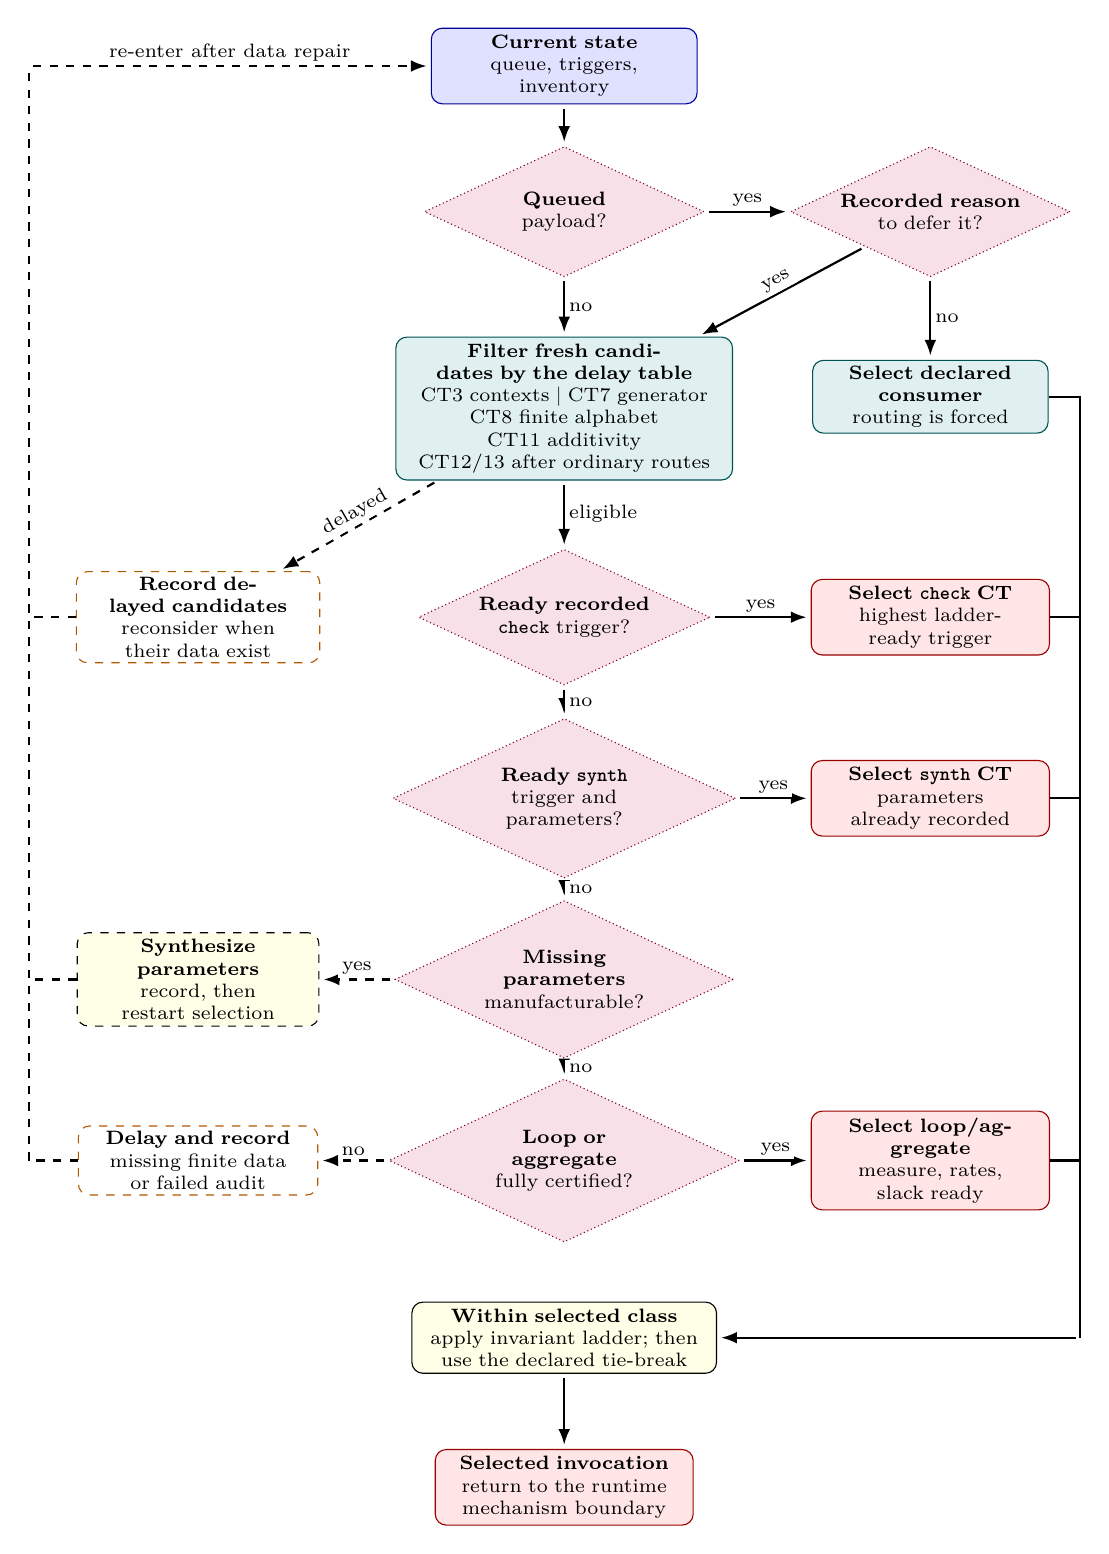
\begin{tikzpicture}[
x=1cm,
y=1cm,
every node/.style={font=\scriptsize}
]
\node[bcwide,bcdefinition,text width=3.20cm,minimum width=3.20cm]
  (state) at (0,0) {\textbf{Current state}\\queue, triggers,\\inventory};
\node[bcdec,bcaudit,text width=2.25cm,minimum width=3.00cm]
  (queue) at (0,-1.85) {\textbf{Queued}\\payload?};
\node[bcdec,bcaudit,text width=2.35cm,minimum width=3.10cm]
  (defer) at (4.65,-1.85) {\textbf{Recorded reason}\\to defer it?};
\node[bcroute,bccorollary,text width=2.85cm,minimum width=2.85cm]
  (consume) at (4.65,-4.20) {\textbf{Select declared consumer}\\routing is forced};
\node[bcwide,bccorollary,text width=4.10cm,minimum width=4.10cm]
  (filter) at (0,-4.35) {\textbf{Filter fresh candidates by the delay table}\\
  CT3 contexts \(\mid\) CT7 generator\\
  CT8 finite alphabet\\
  CT11 additivity\\
  CT12/13 after ordinary routes};
\node[bcdec,bcaudit,text width=2.40cm,minimum width=3.10cm]
  (check) at (0,-7.00) {\textbf{Ready recorded}\\\texttt{check} trigger?};
\node[bcbox,bctheorem,text width=2.85cm,minimum width=2.85cm]
  (runcheck) at (4.65,-7.00) {\textbf{Select \texttt{check} CT}\\highest ladder-ready trigger};
\node[bcroute,bcrouteneutral,bcdesign,text width=2.95cm,minimum width=2.95cm]
  (delayed) at (-4.65,-7.00) {\textbf{Record delayed candidates}\\reconsider when their data exist};
\node[bcdec,bcaudit,text width=2.45cm,minimum width=3.15cm]
  (synthready) at (0,-9.30) {\textbf{Ready \texttt{synth}}\\trigger and parameters?};
\node[bcbox,bctheorem,text width=2.85cm,minimum width=2.85cm]
  (runsynth) at (4.65,-9.30) {\textbf{Select \texttt{synth} CT}\\parameters\\already recorded};
\node[bcdec,bcaudit,text width=2.50cm,minimum width=3.20cm]
  (params) at (0,-11.60) {\textbf{Missing}\\\textbf{parameters}\\manufacturable?};
\node[bcroutepanel,bcdesign,text width=2.90cm,minimum width=2.90cm]
  (makeparams) at (-4.65,-11.60) {\textbf{Synthesize parameters}\\record, then restart selection};
\node[bcdec,bcaudit,text width=2.55cm,minimum width=3.25cm]
  (loopready) at (0,-13.90) {\textbf{Loop or}\\\textbf{aggregate}\\fully certified?};
\node[bcbox,bctheorem,text width=2.85cm,minimum width=2.85cm]
  (runloop) at (4.65,-13.90) {\textbf{Select loop/aggregate}\\measure, rates, slack ready};
\node[bcroute,bcrouteneutral,bcdesign,text width=2.90cm,minimum width=2.90cm]
  (delay) at (-4.65,-13.90) {\textbf{Delay and record}\\missing finite data\\or failed audit};
\node[bcroutepanel,text width=3.70cm,minimum width=3.70cm]
  (tie) at (0,-16.15) {\textbf{Within selected class}\\apply invariant ladder; then\\use the declared tie-break};
\node[bcbox,bctheorem,text width=3.10cm,minimum width=3.10cm]
  (execute) at (0,-18.05) {\textbf{Selected invocation}\\return to the runtime mechanism boundary};
\coordinate (selecttop) at (6.55,-4.20);
\coordinate (selectbus) at (6.55,-16.15);
\coordinate (reentrytop) at (-6.80,0);
\coordinate (reentrybottom) at (-6.80,-13.90);
\draw[bcarr] (state)--(queue);
\draw[bcarr] (queue)--node[bclabel,above]{yes}(defer);
\draw[bcarr] (queue)--node[bclabel,right]{no}(filter);
\draw[bcarr] (defer)--node[bclabel,right]{no}(consume);
\draw[bcarr] (defer)--node[bclabel,above,sloped]{yes}(filter);
\draw[bcarr] (filter)--node[bclabel,right,pos=0.48]{eligible}(check);
\draw[bcrecoverarr] (filter)--node[bclabel,above,sloped,pos=0.48]{delayed}(delayed);
\draw[bcarr] (check)--node[bclabel,above]{yes}(runcheck);
\draw[bcarr] (check)--node[bclabel,right]{no}(synthready);
\draw[bcarr] (synthready)--node[bclabel,above]{yes}(runsynth);
\draw[bcarr] (synthready)--node[bclabel,right]{no}(params);
\draw[bcrecoverarr] (params)--node[bclabel,above]{yes}(makeparams);
\draw[bcarr] (params)--node[bclabel,right]{no}(loopready);
\draw[bcarr] (loopready)--node[bclabel,above]{yes}(runloop);
\draw[bcrecoverarr] (loopready)--node[bclabel,above]{no}(delay);
\draw[thick] (consume.east)--(selecttop)--(selectbus);
\draw[thick] (runcheck.east)--(6.55,-7.00);
\draw[thick] (runsynth.east)--(6.55,-9.30);
\draw[thick] (runloop.east)--(6.55,-13.90);
\draw[bcarr] (selectbus)--(tie.east);
\draw[bcarr] (tie)--(execute);
\draw[thick,dashed] (reentrybottom)--(reentrytop);
\draw[thick,dashed] (delayed.west)--(-6.80,-7.00);
\draw[thick,dashed] (makeparams.west)--(-6.80,-11.60);
\draw[thick,dashed] (delay.west)--(reentrybottom);
\draw[bcrecoverarr] (reentrytop)--node[bclabel,above]{re-enter after data repair}(state.west);
\end{tikzpicture}%
}
\caption[Strategy selection policy]{Strategy selection policy.  A queued payload is consumed unless a reason to defer it is recorded.  Fresh candidates first pass the CT-specific delay table; the first nonempty eligible priority class then supplies the invocation.  Deferred candidates and parameter-repair tasks return to the top only after the missing data are recorded.}
\label{fig:strategy-selection-policy}
\end{figure}

\subsection{Nondeterminism inventory}\label{nondeterminism-inventory}

Genuine strategic freedom is concentrated at a few nodes; below those
nodes execution is forced by the payload type and the entry in \secref{part-ii-the-tactic-library}.

\begingroup
\small
\setlength{\tabcolsep}{2pt}
\begin{longtable}[]{@{}
  >{\raggedright\arraybackslash}p{0.24\linewidth}
  >{\raggedright\arraybackslash}p{0.34\linewidth}
  >{\raggedright\arraybackslash}p{0.34\linewidth}@{}}
\toprule\noalign{}
Node & Options & Deciding test \\
\midrule\noalign{}
\endhead
\bottomrule\noalign{}
\endlastfoot
CT1 target-avoidance fan-out & CT2, CT3, CT4, CT5, CT6, or CT17 payloads. & Hypothesis extraction determines the available payload constructors; if several are certified, apply the selection priority, invariant ladder, and declared tie-break. \\
CT2 minimality route & deletion C2, replacement C2, context residual \(P_{2\to3}\), or target-uncompressible residual \(P_{2\to10}\). & Test hypothesis preservation for deletion, then context-universal replacement; typed failure determines the residual. \\
CT5 local-to-global exit & C4 summation, charge ledger \(P_{5\to4}\), localized deficit \(P_{5\to11}\), or aggregate mass \(P_{5\to14}\). & The certified local witness decides the route: payers give CT4, additive deficit gives CT11, and residual mass gives CT14. \\
CT7 neutral noncompressive branch & CT10 or CT16. & If the missing datum is local and finite, refine; if the support is the whole object with computable closed type, use exact types. \\
CT9 overloaded fibre extraction & Target hit, same-interface exchange, or long chain; any problem-specific matching or star is an intermediate configuration. & Not free once the homogeneous subfamily is chosen; the instantiation lemma maps the configuration to a declared CT9 output. \\
Overload label choice & largest class, extremal class, or predeclared canonical tie-break. & The default is largest class; any other choice must be part of the charge-map definition. \\
CT11 localized deficit route & target-test data \(P_{11\to1}\), exchange data \(P_{11\to7}\), admissibility gap \(P_{11\to10}\), or carried mass \(P_{11\to14}\). & After additivity and admissibility closure, the localized piece's certified structure determines the consumer. \\
CT13 fallback route & tier-one account \(P_{13\to4}\), overlap fibre \(P_{13\to9}\), or overlap mass \(P_{13\to14}\). & The minimal obstruction decides the output: assignable charge, overfull overlap fibre, or residual overlap mass. \\
Aggregate versus pointwise treatment & CT14 aggregate closure, CT9 overload, or CT10 label refinement. & Select CT14 only when class mass, per-member capacity, and multiplicity records are available; use CT9 for a named overload and CT10 when the missing ingredient is a bounded finite capacity label.  Once CT14 is admitted, its local audit returns C4, \(P_{14\to9}\), \(P_{14\to10}\), or the declared scope boundary. \\
CT16 exact-type escalation & C2 exact identification, proper-piece response \(P_{16\to3}\), or distinct closed datum \(P_{16\to10}\). & Escalate only when local support no longer separates the object and the closed type is computable. \\
Budget failure after empty rate interval & sharpen supply, split demand into a tier, or localize deficit. & The slack/interlock table identifies which inequality is binding. \\
\end{longtable}
\endgroup

This table is where the human mathematician or supervised model sits.
The remaining work is delegated to admitted tactic invocations and their
worksheets.

Figure~\ref{fig:strategy-nondeterminism-inventory} displays the main
choice nodes in the nondeterminism inventory.

\begin{figure}[htbp]
\centering
\resizebox{0.98\textwidth}{!}{%
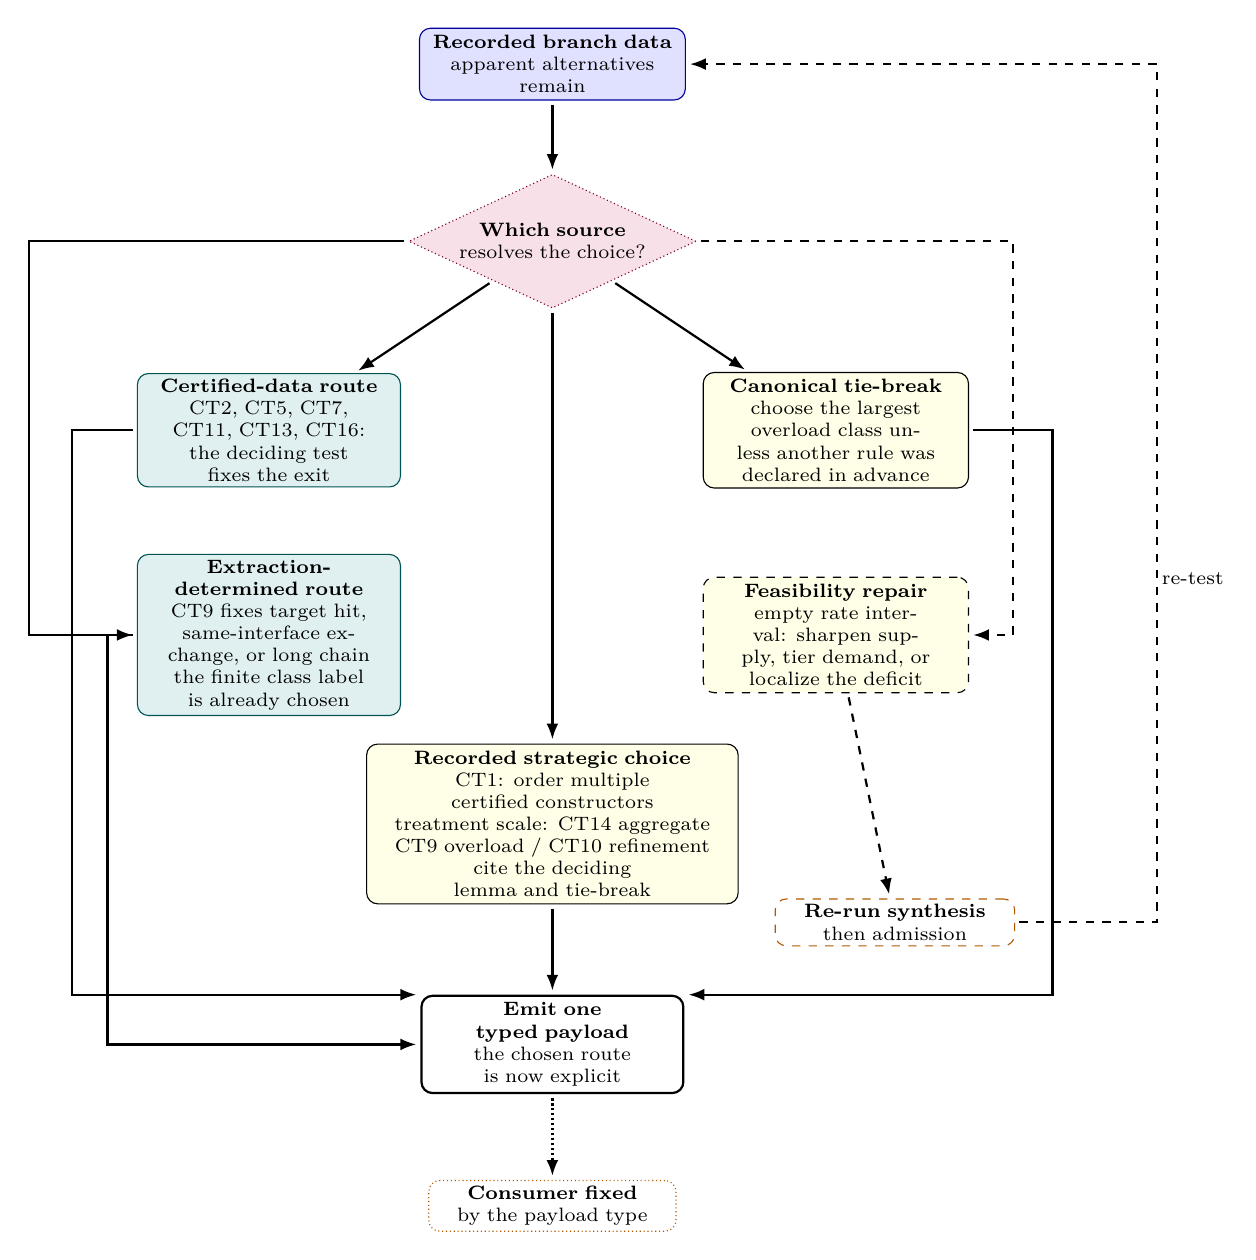
\begin{tikzpicture}[
x=1cm,
y=1cm,
every node/.style={font=\scriptsize}
]
\node[bcwide,bcdefinition,text width=3.20cm,minimum width=3.20cm]
  (branch) at (0,0) {\textbf{Recorded branch data}\\apparent alternatives\\remain};
\node[bcdec,bcaudit,text width=2.45cm,minimum width=3.20cm]
  (kind) at (0,-2.25) {\textbf{Which source}\\resolves the choice?};
\node[bcroute,bccorollary,text width=3.20cm,minimum width=3.20cm]
  (evidence) at (-3.60,-4.65) {\textbf{Certified-data route}\\CT2, CT5, CT7, CT11, CT13, CT16:\\the deciding test fixes the exit};
\node[bcroute,bccorollary,text width=3.20cm,minimum width=3.20cm]
  (shape) at (-3.60,-7.25) {\textbf{Extraction-determined route}\\CT9 fixes target hit, same-interface exchange, or long chain\\the finite class label is already chosen};
\node[bcroutepanel,text width=3.20cm,minimum width=3.20cm]
  (tie) at (3.60,-4.65) {\textbf{Canonical tie-break}\\choose the largest overload class unless another rule was declared in advance};
\node[bcroutepanel,bcdesign,text width=3.20cm,minimum width=3.20cm]
  (repair) at (3.60,-7.25) {\textbf{Feasibility repair}\\empty rate interval: sharpen supply, tier demand, or localize the deficit};
\node[bcroutepanel,text width=4.55cm,minimum width=4.55cm]
  (supervised) at (0,-9.65) {\textbf{Recorded strategic choice}\\
  CT1: order multiple certified constructors\\
  treatment scale: CT14 aggregate\\
  CT9 overload / CT10 refinement\\
  cite the deciding lemma and tie-break};
\node[bcbox,bcpayload,text width=3.15cm,minimum width=3.15cm]
  (payload) at (0,-12.45) {\textbf{Emit one typed payload}\\the chosen route is now explicit};
\node[bcroute,bcrouteneutral,bcoutputroute,text width=3.00cm,minimum width=3.00cm]
  (consumer) at (0,-14.50) {\textbf{Consumer fixed}\\by the payload type};
\node[bcroute,bcrouteneutral,bcdesign,text width=2.90cm,minimum width=2.90cm]
  (reevaluate) at (4.35,-10.90) {\textbf{Re-run synthesis}\\then admission};
\draw[bcarr] (branch)--(kind);
\draw[bcarr] (kind)--(evidence);
\draw[bcarr] (kind.west) -- (-6.65,-2.25) |- (shape.west);
\draw[bcarr] (kind)--(tie);
\draw[bcrecoverarr] (kind.east) -- (5.85,-2.25) |- (repair.east);
\draw[bcarr] (kind)--(supervised);
\draw[bcarr] (evidence.west)--(-6.10,-4.65)|-(payload.north west);
\draw[bcarr] (shape.west)--(-5.65,-7.25)|-(payload.west);
\draw[bcarr] (tie.east)--(6.35,-4.65)|-(payload.north east);
\draw[bcarr] (supervised)--(payload);
\draw[bchandoff] (payload)--(consumer);
\draw[bcrecoverarr] (repair)--(reevaluate);
\draw[bcrecoverarr] (reevaluate.east) -- ++(1.80,0) |- node[bclabel,right,pos=0.20]{re-test} (branch.east);
\end{tikzpicture}%
}
\caption[Strategy nondeterminism inventory]{Strategy nondeterminism inventory.  Certified residuals and extraction lemmas force most exits.  Strategic freedom remains when CT1 certifies several constructors, when aggregate and pointwise treatments compete, or when a canonical label tie-break is required.  Each such choice is recorded before one typed payload fixes the consumer.}
\label{fig:strategy-nondeterminism-inventory}
\end{figure}

\subsection{Parameter synthesis}\label{parameter-synthesis}

Every Parameters slot in \secref{part-ii-the-tactic-library} points to one synthesis rule here. The
rules are organized by parameter type.  Choices of charging scale,
activity threshold, finite alphabet, next missing invariant, rank notion,
well-founded measure, and offset family are made here; the CT entries
then consume the recorded data mechanically.

\textbf{15.1 Resource inventory.} Compile the available minimality
tools, local test algebra, external black boxes, charging resources,
finite label alphabets, type tables, and closed routes. Reject a
proposal whose positive or negative branch cannot be paid from this
inventory. Feeds: all triggers; especially CT2, CT4, CT5, CT11, CT15.

\textbf{15.2 Invariants and labels.} Use hypothesis extraction: the
invariant is the hypothesis of the lemma one wants to apply, and the
failure of that hypothesis must already route to a CT payload. The seven
mechanical sources are threshold equations, minimality consequences,
type distinctions, label refinements, first failures, saturation
conditions, and finite-table cutoffs. Feeds: label slots of CT8, CT9,
CT10, CT13, CT17 and branch-state predicates for all CTs.

\textbf{15.3 Types and generators.} Produce certified finite context
generators, exact external types, and closed whole-object types. The
audit obligation is equivalence: the generator or type must decide all
compatible contexts relevant to the target. Feeds: CT3, CT7, CT8, CT16.

\textbf{15.4 Budgets and rates.} Choose currencies, put the budget in
normal form, compute the rate interval backwards, and record both
endpoints and slack. Solved threshold equations become new invariants.
Feeds: CT4, CT5, CT11, CT14, CT15.

\textbf{15.5 Measures.} A loop or cyclic handoff requires a
well-founded measure that decreases on each pass after the branch state
is restored. Feeds: CT12 and any cyclic combinator edge.

\textbf{15.6 Synthesis audits.} Run monotonicity of every move against
every budget, separation of supply accounts, and slack-consumption
checks before the tactic is selected. These audits feed the worksheet's
Artifacts and Open items fields.

\textbf{Bijection claim.} Every parameter slot in \secref{part-ii-the-tactic-library} must cite exactly
one rule among 15.1--15.6, and every rule above lists its consuming CT
slots. A slot with no rule is synthesis folklore; a rule with no
consumer is unused bureaucracy.

\begingroup
\scriptsize
\setlength{\tabcolsep}{1.4pt}
\begin{longtable}[]{@{}
  >{\raggedright\arraybackslash}p{0.16\linewidth}
  >{\raggedright\arraybackslash}p{0.20\linewidth}
  >{\raggedright\arraybackslash}p{0.30\linewidth}
  >{\raggedright\arraybackslash}p{0.26\linewidth}@{}}
\toprule\noalign{}
Rule & Parameter family & Consuming slots & Inverse check \\
\midrule\noalign{}
\endhead
\bottomrule\noalign{}
\endlastfoot
15.1 & Resource inventory, admissibility class, minimality tools, replacement family. & CT1 witness inventory; CT2 size order, admissibility, replacements; CT4 payer resources; CT5 summation domain; CT11 admissibility class; CT15 independent coordinates. & Every entry using a proof resource cites the inventory before execution. \\
15.2 & Invariants, finite labels, branch predicates, first-failure flags. & CT1 branch-state record; CT6 activity predicate and threshold flag; CT8 label alphabet; CT9 fibre label map; CT10 refined label alphabet; CT13 tier labels; CT17 survivor labels. & Every finite label or branch predicate is a recorded invariant or label source. \\
15.3 & Context generators, external types, exact closed types, response evaluators. & CT3 context universe/type evaluator; CT7 context generator and response evaluator; CT8 exact type equality test; CT16 closed-type evaluator. & Every context-equivalence or exact-type obligation has a generator/type rule. \\
15.4 & Budgets, ledgers, capacities, rates, slack records. & CT4 canonical map/capacity/lower bound; CT5 local lower bound; CT11 budget; CT14 mass and capacity bounds; CT15 full-rank ledger; CT17 arithmetic threshold and residual-mass bound. & Every quantitative comparison reads a budget/rate/slack entry. \\
15.5 & Well-founded measures for loops and cyclic routes. & CT12 peel measure; CT13 tier reconciliation loops; cyclic typed-handoff combinators. & Every repeated route carries S-Meas or is rejected. \\
15.6 & Synthesis audits: monotonicity, separation, slack, restoration. & Audit hooks for CT4, CT5, CT11, CT12, CT13, CT14, CT15, and worksheet Artifact/Open-item fields. & Every synthesized parameter writes an audit row or a defect-register reject. \\
\end{longtable}
\endgroup

Figure~\ref{fig:strategy-parameter-synthesis} displays the parameter
synthesis workflow.

\begin{figure}[htbp]
\centering
\resizebox{0.87\textwidth}{!}{%
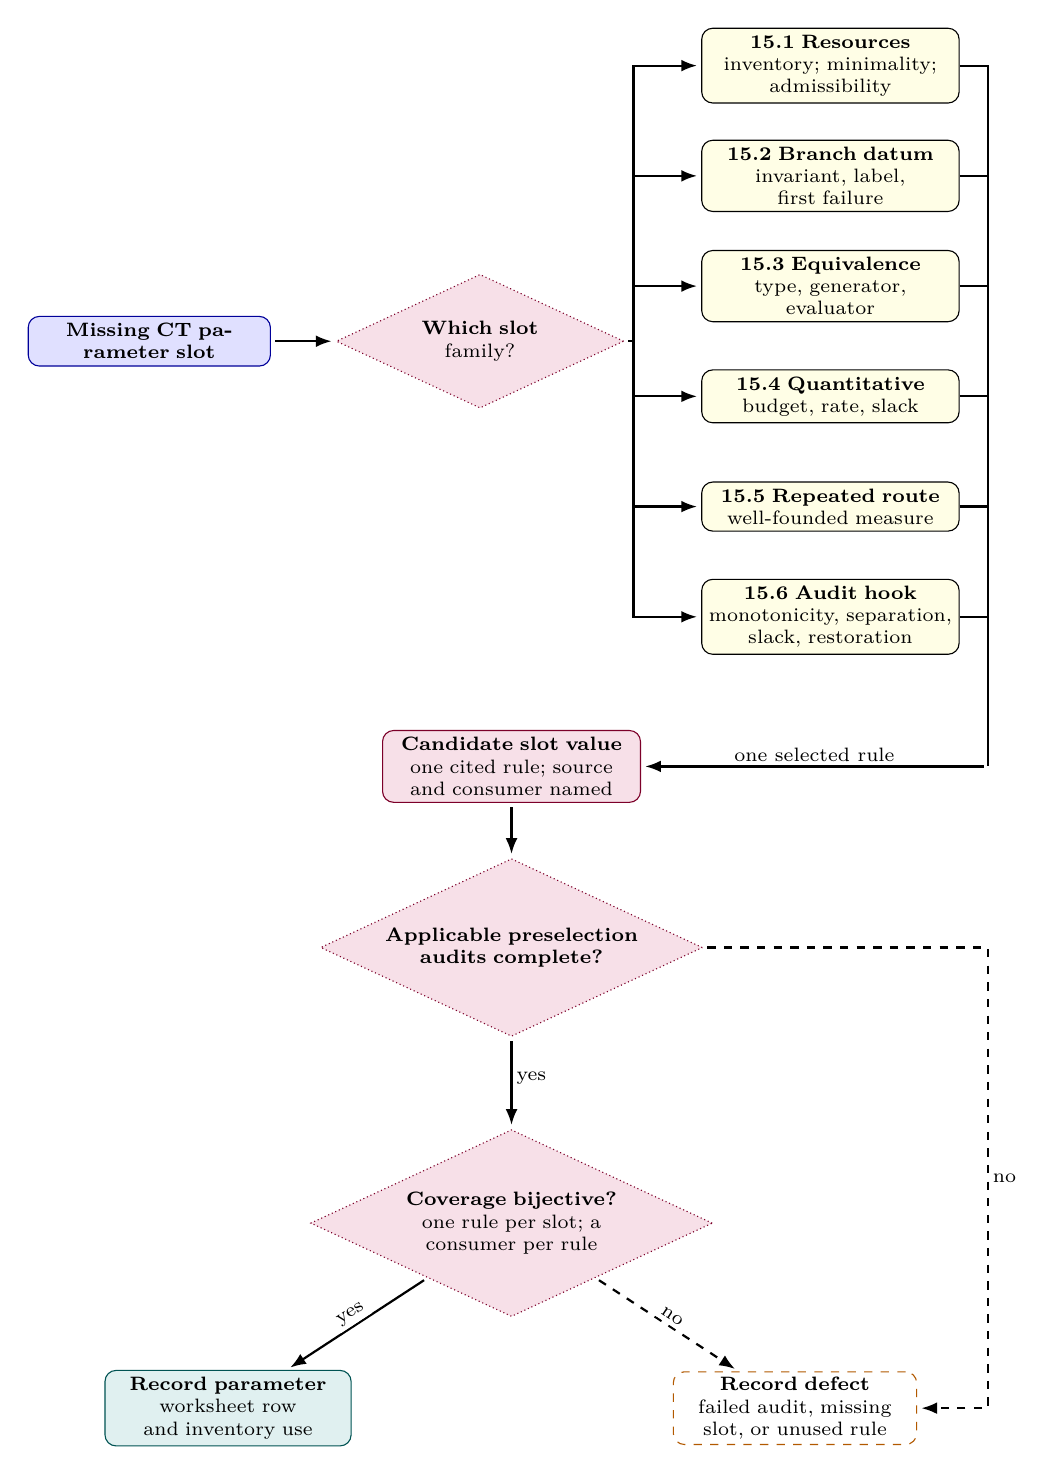
\begin{tikzpicture}[
x=1cm,
y=1cm,
every node/.style={font=\scriptsize}
]
\node[bcwide,bcdefinition,text width=2.90cm,minimum width=2.90cm]
  (slot) at (-4.60,0) {\textbf{Missing CT parameter slot}};
\node[bcdec,bcaudit,text width=2.35cm,minimum width=3.10cm]
  (family) at (-0.40,0) {\textbf{Which slot}\\family?};
\node[bcroutepanel,text width=3.10cm,minimum width=3.10cm]
  (r1) at (4.05,3.50) {\textbf{15.1 Resources}\\inventory; minimality;\\admissibility};
\node[bcroutepanel,text width=3.10cm,minimum width=3.10cm]
  (r2) at (4.05,2.10) {\textbf{15.2 Branch datum}\\invariant, label,\\first failure};
\node[bcroutepanel,text width=3.10cm,minimum width=3.10cm]
  (r3) at (4.05,0.70) {\textbf{15.3 Equivalence}\\type, generator,\\evaluator};
\node[bcroutepanel,text width=3.10cm,minimum width=3.10cm]
  (r4) at (4.05,-0.70) {\textbf{15.4 Quantitative}\\budget, rate, slack};
\node[bcroutepanel,text width=3.10cm,minimum width=3.10cm]
  (r5) at (4.05,-2.10) {\textbf{15.5 Repeated route}\\well-founded measure};
\node[bcroutepanel,text width=3.10cm,minimum width=3.10cm]
  (r6) at (4.05,-3.50) {\textbf{15.6 Audit hook}\\monotonicity, separation,\\slack, restoration};
\node[bcbox,bclemma,text width=3.10cm,minimum width=3.10cm]
  (candidate) at (0,-5.40) {\textbf{Candidate slot value}\\one cited rule; source and consumer named};
\node[bcdec,bcaudit,text width=3.55cm,minimum width=4.25cm]
  (audit) at (0,-7.70) {\textbf{Applicable preselection}\\\textbf{audits complete?}};
\node[bcdec,bcaudit,text width=3.20cm,minimum width=3.90cm]
  (coverage) at (0,-11.20) {\textbf{Coverage bijective?}\\one rule per slot; a consumer per rule};
\node[bcbox,bccorollary,text width=2.95cm,minimum width=2.95cm]
  (record) at (-3.60,-13.55) {\textbf{Record parameter}\\worksheet row and inventory use};
\node[bcroute,bcrouteneutral,bcdesign,text width=2.95cm,minimum width=2.95cm]
  (defect) at (3.60,-13.55) {\textbf{Record defect}\\failed audit, missing slot, or unused rule};
\coordinate (rulebus) at (6.05,-5.40);
\draw[bcarr] (slot)--(family);
\draw[bcarr] (family.east) -- (1.55,0) |- (r1.west);
\draw[bcarr] (family.east) -- (1.55,0) |- (r2.west);
\draw[bcarr] (family.east) -- (1.55,0) |- (r3.west);
\draw[bcarr] (family.east) -- (1.55,0) |- (r4.west);
\draw[bcarr] (family.east) -- (1.55,0) |- (r5.west);
\draw[bcarr] (family.east) -- (1.55,0) |- (r6.west);
\draw[thick] (r1.east)--(6.05,3.50)--(rulebus);
\draw[thick] (r2.east)--(6.05,2.10);
\draw[thick] (r3.east)--(6.05,0.70);
\draw[thick] (r4.east)--(6.05,-0.70);
\draw[thick] (r5.east)--(6.05,-2.10);
\draw[thick] (r6.east)--(6.05,-3.50);
\draw[bcarr] (rulebus)--node[bclabel,above]{one selected rule}(candidate.east);
\draw[bcarr] (candidate)--(audit);
\draw[bcarr] (audit)--node[bclabel,right,pos=0.45]{yes}(coverage);
\draw[bcrecoverarr] (audit.east) -- (6.05,-7.70) |- node[bclabel,right,pos=0.25]{no}(defect.east);
\draw[bcarr] (coverage)--node[bclabel,above,sloped]{yes}(record);
\draw[bcrecoverarr] (coverage)--node[bclabel,above,sloped]{no}(defect);
\end{tikzpicture}%
}
\caption[Strategy parameter synthesis]{Strategy parameter synthesis.  The slot type selects exactly one rule family among 15.1--15.6 for this filling pass.  Outputs may become inputs to later passes---for example, a solved rate threshold becomes a recorded invariant---but each slot cites one rule.  The resulting value then passes the applicable preselection audits and the slot--rule coverage check.}
\label{fig:strategy-parameter-synthesis}
\end{figure}
\FloatBarrier
\clearpage

\subsection{Combinators}\label{combinators}

Combinators organize tactic invocations but are not closure tactics,
because they produce neither a certificate nor a smaller residual by
themselves.

\begingroup
\small
\setlength{\tabcolsep}{2pt}
\begin{longtable}[]{@{}
  >{\raggedright\arraybackslash}p{0.18\linewidth}
  >{\raggedright\arraybackslash}p{0.28\linewidth}
  >{\raggedright\arraybackslash}p{0.28\linewidth}
  >{\raggedright\arraybackslash}p{0.18\linewidth}@{}}
\toprule\noalign{}
Combinator & Signature & Obligations & Formal counterpart \\
\midrule\noalign{}
\endhead
\bottomrule\noalign{}
\endlastfoot
Sequencing / spine & ordered invocations \(I_1,\ldots,I_m\) with later triggers depending on earlier outputs & ladder order, no backward hypothesis consumption, S-Meas on cycles & proof script with dependency order \\
Typed handoff & payload \(P_{i\to j}\) emitted by CT\(i\) and consumed by CT\(j\) & routing at source, trigger at target, branch-table row & typed term passed between lemmas \\
Black-box isolation & external theorem plus constants and interface contract & cited theorem, constant interlock, trust-base register & imported axiom or theorem namespace \\
\end{longtable}
\endgroup

The admission test keeping a construct out of \secref{part-ii-the-tactic-library} is decisive: a
CT entry must return C1--C5 or emit a legal typed payload. A cyclic route
must additionally satisfy the measure requirement stated in its
canonical entry. Otherwise the construct is a combinator or an
assurance artifact, not a CT entry.

Figure~\ref{fig:strategy-combinators} displays the combinator
classification workflow.

\begin{figure}[htbp]
\centering
\resizebox{0.98\textwidth}{!}{%
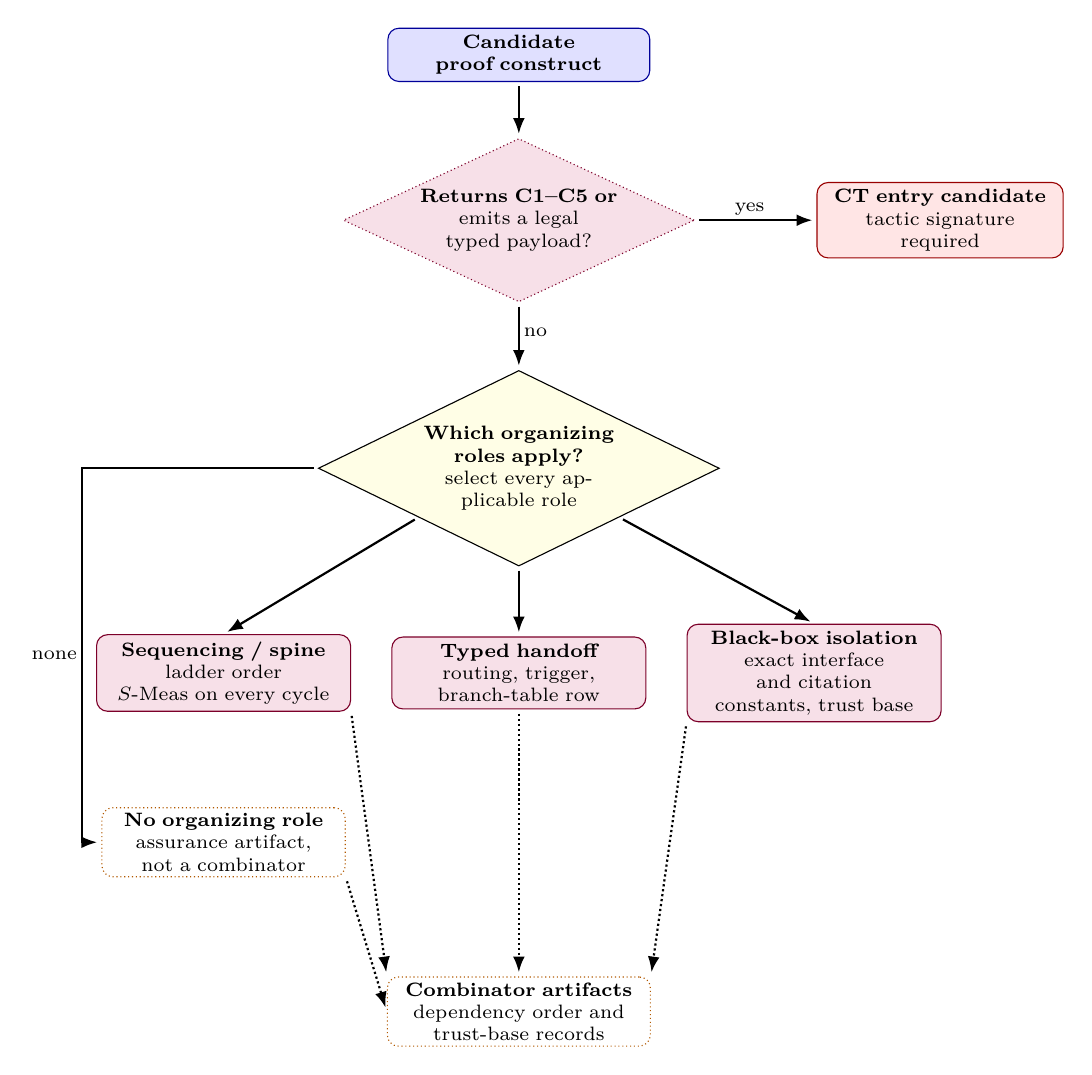
\begin{tikzpicture}[
x=1cm,
y=1cm,
every node/.style={font=\scriptsize}
]
\node[bcwide,bcdefinition,text width=3.15cm,minimum width=3.15cm]
  (candidate) at (0,0) {\textbf{Candidate proof construct}};
\node[bcdec,bcaudit,text width=2.55cm,minimum width=3.25cm]
  (ctgate) at (0,-2.10) {\textbf{Returns C1--C5 or}\\emits a legal typed payload?};
\node[bcbox,bctheorem,text width=2.95cm,minimum width=2.95cm]
  (ctentry) at (5.35,-2.10) {\textbf{CT entry candidate}\\tactic signature\\required};
\node[bcroutechoice,text width=2.70cm,minimum width=3.45cm]
  (roles) at (0,-5.25) {\textbf{Which organizing}\\\textbf{roles apply?}\\select every applicable role};
\node[bcbox,bclemma,text width=3.05cm,minimum width=3.05cm]
  (seq) at (-3.75,-7.85) {\textbf{Sequencing / spine}\\ladder order\\\(S\)-Meas on every cycle};
\node[bcbox,bclemma,text width=3.05cm,minimum width=3.05cm]
  (handoff) at (0,-7.85) {\textbf{Typed handoff}\\routing, trigger, branch-table row};
\node[bcbox,bclemma,text width=3.05cm,minimum width=3.05cm]
  (blackbox) at (3.75,-7.85) {\textbf{Black-box isolation}\\exact interface and citation\\constants, trust base};
\node[bcroute,bcrouteneutral,bcoutputroute,text width=2.95cm,minimum width=2.95cm]
  (assurance) at (-3.75,-10.00) {\textbf{No organizing role}\\assurance artifact, not a combinator};
\node[bcroute,bcrouteneutral,bcoutputroute,text width=3.20cm,minimum width=3.20cm]
  (audit) at (0,-12.15) {\textbf{Combinator artifacts}\\dependency order and trust-base records};
\draw[bcarr] (candidate)--(ctgate);
\draw[bcarr] (ctgate.east)--node[bclabel,above,pos=0.45]{yes}(ctentry.west);
\draw[bcarr] (ctgate.south)--node[bclabel,right,pos=0.45]{no}(roles.north);
\draw[bcarr] (roles.south west)--(seq.north);
\draw[bcarr] (roles.south)--(handoff.north);
\draw[bcarr] (roles.south east)--(blackbox.north);
\draw[bcarr] (roles.west) -- (-5.55,-5.25) |- node[bclabel,left,pos=0.25]{none}(assurance.west);
\draw[bchandoff] (seq.south east)--(audit.north west);
\draw[bchandoff] (handoff.south)--(audit.north);
\draw[bchandoff] (blackbox.south west)--(audit.north east);
\draw[bchandoff] (assurance.south east)--(audit.west);
\end{tikzpicture}%
}
\caption[Strategy combinators]{Strategy combinators.  A construct is a CT candidate only when it returns C1--C5 or a legal typed payload; cyclic routes must also satisfy their recorded measure requirement.  Otherwise the strategy selects every applicable organizing role.  If no organizing role applies, the construct is an assurance artifact rather than a combinator.}
\label{fig:strategy-combinators}
\end{figure}

\subsection{Advanced closure
patterns}\label{advanced-closure-patterns}

The following patterns manage dependencies spanning several tactic
invocations. They record sequencing, typed handoffs, or black-box
imports together with the associated assurance artifacts.

\subsubsection{Branch sequencing and derived
normalizations}\label{branch-sequencing-and-derived-normalizations}

Estimates frequently hold under a normalization --- a density,
regularity, or budget hypothesis about \(G\). The normalization is
\textbf{derived}: the branch on which the normalization fails is
exhausted \emph{before} any estimate depending on it is invoked. The
result is a \textbf{spine}: the surviving branch on which all
normalizations have been either derived or made unnecessary, and along
which the main quantitative estimates are valid.

The design rule is explicit sequencing: the proof declares the order in
which conditional branches are discharged, and every estimate names the
branch state on which it is valid. A normalization-failure branch must
itself terminate in the standard taxonomy: a routed exit, a charged
demand, or the derived normalization itself as its third alternative.
The normalization-failure branch uses only
estimates available before the normalization. The dependency order is
part of the proof and is recorded in the artifacts of \secref{proof-engineering-artifacts}.

\subsubsection{Typed handoffs between
branches}\label{typed-handoffs-between-branches}

Large branch systems require branches to delegate to one another. A
\textbf{typed handoff} is an inter-branch interface with a declared data
format. The source establishes that its output has the registered
payload type and records the route; the receiving trigger must follow
from that payload, and inherited branch data must remain available. The
dependency artifacts (\secref{proof-engineering-artifacts}) record the handoff as a directed
edge with its payload.

Handoffs may be cyclic at the diagram level (branch A hands to B, whose
residual re-enters A's saturation test). The declared measure then proves
termination of the cycle as in \secref{peeling-loops-closure-by-well-founded-recursion}; restored branch data
must also match the state expected at re-entry. An invocation that uses
another branch's conclusion without the registered payload, trigger, or
state transport remains an unresolved dependency.



\subsubsection{Black-box isolation of external
inputs}\label{black-box-isolation-of-external-inputs}

External theorems imported into the proof are \textbf{black boxes}. Each
is stated once, with its exact interface (hypotheses consumed,
conclusion supplied), and listed in a dedicated external-inputs
register. The proof consumes a black box through its declared interface.

This serves three purposes: the trust base of the proof is enumerable at
a glance; a strengthening or weakening of the external theorem can be
impact-checked through the register; and external material remains cited
at the point where the proof consumes it. The admission audit rejects an
interface stronger than the cited theorem. The register entry cites the
exact source statement.

In the Erdős--Gyárfás instantiation, the \(P_{13}\)-free theorem of
Hegde--Sandeep--Shashank is the representative black box: it is used for
precisely the hereditary-class conclusion it proves and remains isolated
from unrelated branch closures \citep{hegde-etal-2024-p13}.

\FloatBarrier
\clearpage

\subsection{Opening script and strategy narratives}\label{opening-script-and-strategy-narratives}

An in-scope instantiation begins by admitting CT1 for the target
predicate and local test family. If a test is realized, it halts at C1.
On the target-avoiding branch, each certified datum proposes its
corresponding payload: a proper piece to CT2, boundary response to CT3,
charge ledger to CT4, local-site family to CT5, activity setup to CT6,
or sparse offset data to CT17. If several constructors are certified,
the selection policy and invariant ladder order the simultaneous
proposals. Each choice is justified by the nondeterminism inventory, not
by the CT1 entry.

A representative strategy thread reaches CT7 by
\[
\text{CT1}\to\text{CT4}\to\text{CT9}\to\text{CT7}.
\]
The CT7 invocation then returns C1, C2, or C3, or one of the registered
typed routes
\[
\begin{gathered}
P_{7\to3}\to\text{CT3},\qquad
P_{7\to12}\to\text{CT12},\\
P_{7\to10}\to\text{CT10},\qquad
P_{7\to16}\to\text{CT16}.
\end{gathered}
\]
On this representative route, CT1 proposes the demand/payer payload only
after a recorded local-density lemma supplies the demand family and its
payers. CT4 is selected because the ledger is already synthesized; CT9
is forced when a fibre overload appears; CT7 is selected because the
homogeneous fibre contains a bounded same-interface exchange. Once each
invocation is admitted, its internal proof is the corresponding
mechanism of \secref{part-ii-the-tactic-library}.

Figure~\ref{fig:strategy-opening-script} displays the opening script and
the representative strategy thread.

\begin{figure}[htbp]
\centering
\resizebox{0.85\textwidth}{!}{%
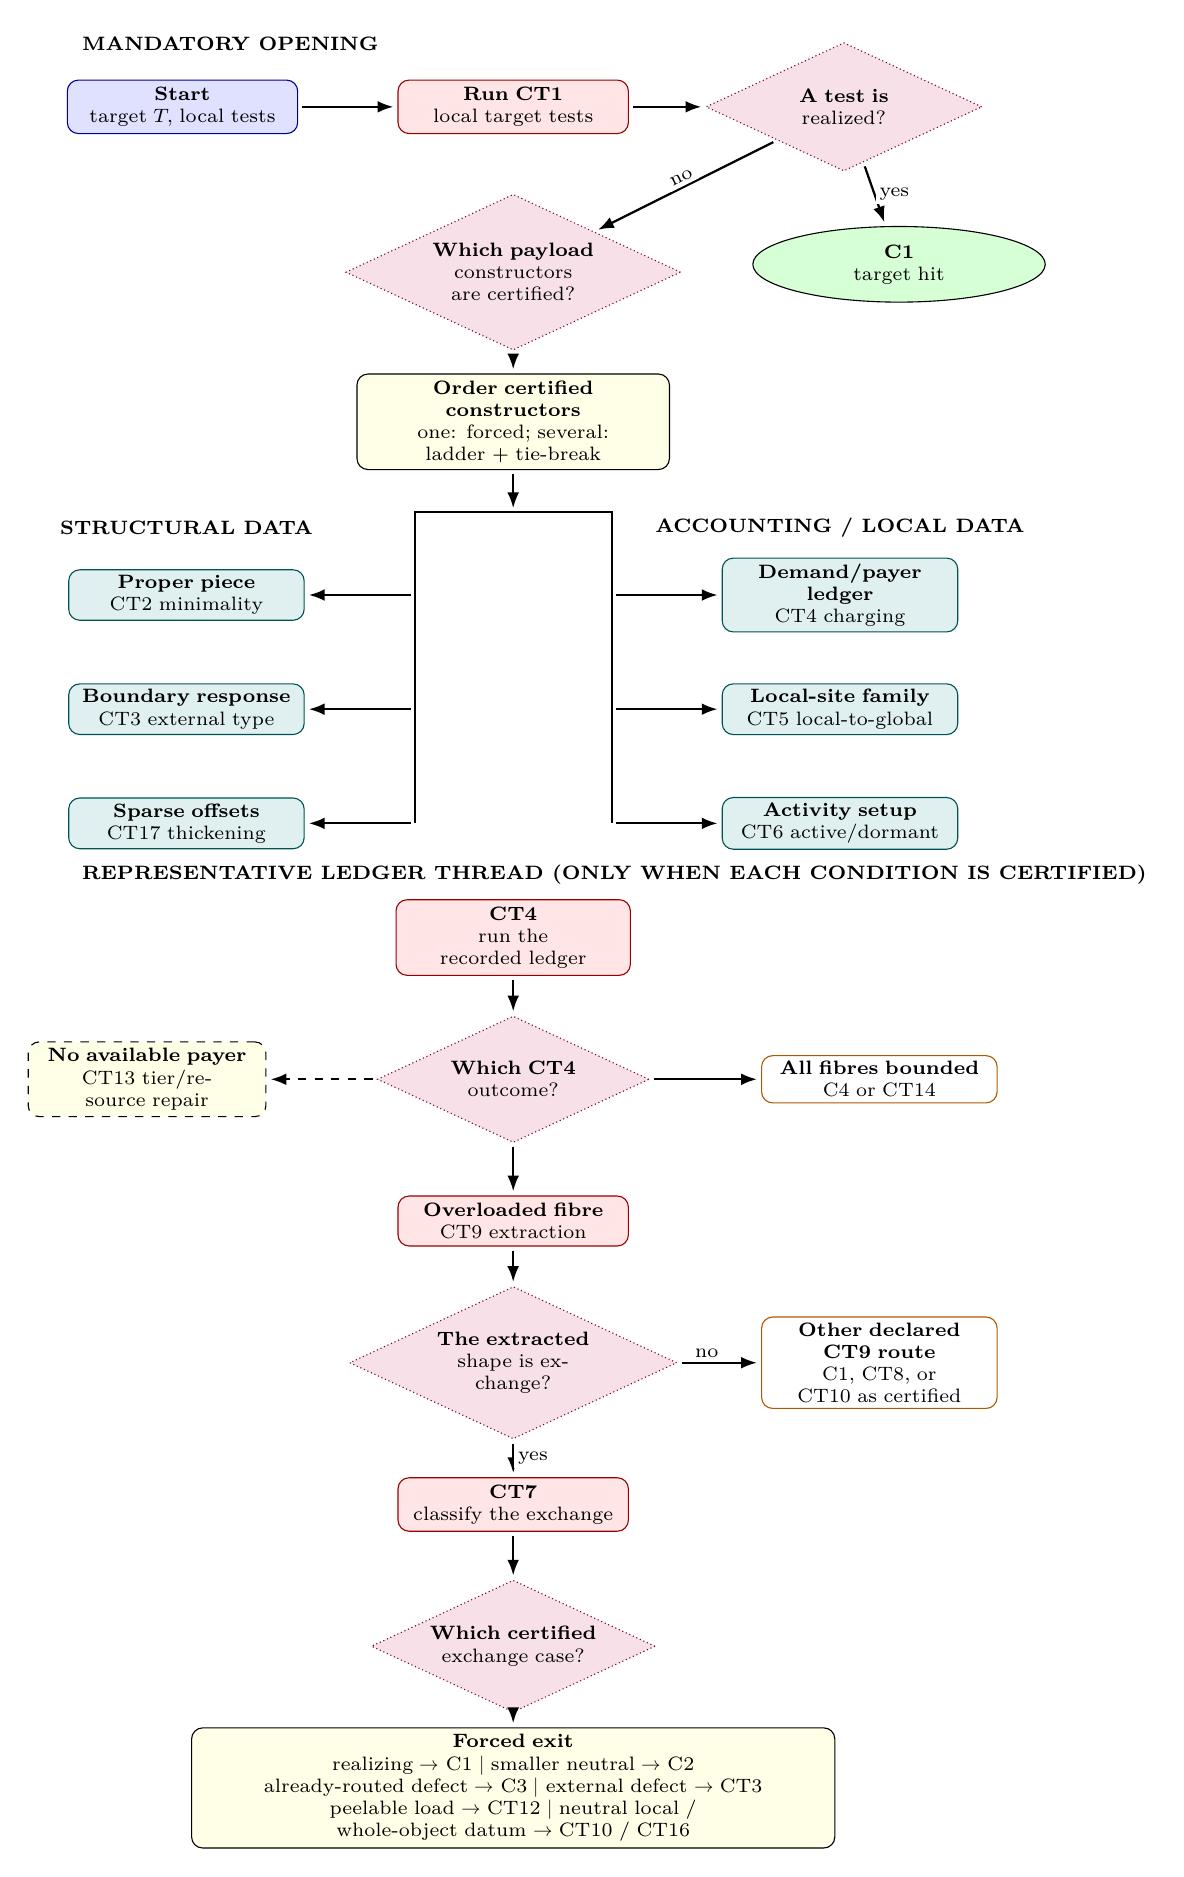
\begin{tikzpicture}[
x=1cm,
y=1cm,
every node/.style={font=\scriptsize}
]
\node[font=\scriptsize\bfseries,anchor=west] at (-5.60,0.80)
  {MANDATORY OPENING};
\node[bcwide,bcdefinition,text width=2.75cm,minimum width=2.75cm]
  (start) at (-4.20,0) {\textbf{Start}\\target \(T\), local tests};
\node[bcbox,bctheorem,text width=2.75cm,minimum width=2.75cm]
  (ct1) at (0,0) {\textbf{Run CT1}\\local target tests};
\node[bcdec,bcaudit,text width=2.30cm,minimum width=3.00cm]
  (hit) at (4.20,0) {\textbf{A test is}\\realized?};
\node[bcclosed,text width=2.45cm,minimum width=2.45cm]
  (c1) at (4.90,-2.00) {\textbf{C1}\\target hit};
\node[bcdec,bcaudit,text width=2.45cm,minimum width=3.15cm]
  (available) at (0,-2.10) {\textbf{Which payload}\\constructors are certified?};
\node[bcroutepanel,text width=3.80cm,minimum width=3.80cm]
  (order) at (0,-4.00) {\textbf{Order certified}\\\textbf{constructors}\\one: forced; several: ladder + tie-break};
\coordinate (ordersplit) at (0,-5.15);
\node[font=\scriptsize\bfseries] at (-4.15,-5.35) {STRUCTURAL DATA};
\node[font=\scriptsize\bfseries] at (4.15,-5.35) {ACCOUNTING / LOCAL DATA};
\node[bcroute,bccorollary,text width=2.85cm,minimum width=2.85cm]
  (ct2) at (-4.15,-6.20) {\textbf{Proper piece}\\CT2 minimality};
\node[bcroute,bccorollary,text width=2.85cm,minimum width=2.85cm]
  (ct3) at (-4.15,-7.65) {\textbf{Boundary response}\\CT3 external type};
\node[bcroute,bccorollary,text width=2.85cm,minimum width=2.85cm]
  (ct17) at (-4.15,-9.10) {\textbf{Sparse offsets}\\CT17 thickening};
\node[bcroute,bccorollary,text width=2.85cm,minimum width=2.85cm]
  (ct4) at (4.15,-6.20) {\textbf{Demand/payer ledger}\\CT4 charging};
\node[bcroute,bccorollary,text width=2.85cm,minimum width=2.85cm]
  (ct5) at (4.15,-7.65) {\textbf{Local-site family}\\CT5 local-to-global};
\node[bcroute,bccorollary,text width=2.85cm,minimum width=2.85cm]
  (ct6) at (4.15,-9.10) {\textbf{Activity setup}\\CT6 active/dormant};
\node[font=\scriptsize\bfseries,anchor=west] at (-5.60,-9.75)
  {REPRESENTATIVE LEDGER THREAD (ONLY WHEN EACH CONDITION IS CERTIFIED)};
\node[bcbox,bctheorem,text width=2.80cm,minimum width=2.80cm]
  (ct4example) at (0,-10.55) {\textbf{CT4}\\run the recorded ledger};
\node[bcdec,bcaudit,text width=2.25cm,minimum width=2.95cm]
  (ct4out) at (0,-12.35) {\textbf{Which CT4}\\outcome?};
\node[bcroutepanel,bcdesign,text width=2.85cm,minimum width=2.85cm]
  (ct13) at (-4.65,-12.35) {\textbf{No available payer}\\CT13 tier/resource repair};
\node[bcroute,bcrouteneutral,text width=2.85cm,minimum width=2.85cm]
  (otherct4) at (4.65,-12.35) {\textbf{All fibres bounded}\\C4 or CT14};
\node[bcbox,bctheorem,text width=2.75cm,minimum width=2.75cm]
  (ct9) at (0,-14.15) {\textbf{Overloaded fibre}\\CT9 extraction};
\node[bcdec,bcaudit,text width=2.25cm,minimum width=2.95cm]
  (exchange) at (0,-15.95) {\textbf{The extracted}\\shape is exchange?};
\node[bcroute,bcrouteneutral,text width=2.85cm,minimum width=2.85cm]
  (otherct9) at (4.65,-15.95) {\textbf{Other declared CT9 route}\\C1, CT8, or CT10 as certified};
\node[bcbox,bctheorem,text width=2.75cm,minimum width=2.75cm]
  (ct7) at (0,-17.75) {\textbf{CT7}\\classify the exchange};
\node[bcdec,bcaudit,text width=2.30cm,minimum width=3.00cm]
  (exchangeout) at (0,-19.55) {\textbf{Which certified}\\exchange case?};
\node[bcroutepanel,text width=8.00cm,minimum width=8.00cm]
  (exits) at (0,-21.35) {\textbf{Forced exit}\\
  realizing \(\to\) C1 \(\mid\) smaller neutral \(\to\) C2\\
  already-routed defect \(\to\) C3 \(\mid\) external defect \(\to\) CT3\\
  peelable load \(\to\) CT12 \(\mid\) neutral local / whole-object datum \(\to\) CT10 / CT16};
\draw[bcarr] (start)--(ct1);
\draw[bcarr] (ct1)--(hit);
\draw[bcarr] (hit)--node[bclabel,right]{yes}(c1);
\draw[bcarr] (hit)--node[bclabel,above,sloped]{no}(available);
\draw[bcarr] (available)--(order);
\draw[bcarr] (order.south)--(ordersplit);
\draw[thick] (ordersplit)--(-1.25,-5.15)--(-1.25,-9.10);
\draw[bcarr] (-1.25,-6.20)--(ct2.east);
\draw[bcarr] (-1.25,-7.65)--(ct3.east);
\draw[bcarr] (-1.25,-9.10)--(ct17.east);
\draw[thick] (ordersplit)--(1.25,-5.15)--(1.25,-9.10);
\draw[bcarr] (1.25,-6.20)--(ct4.west);
\draw[bcarr] (1.25,-7.65)--(ct5.west);
\draw[bcarr] (1.25,-9.10)--(ct6.west);
\draw[bcarr] (ct4example)--(ct4out);
\draw[bcrecoverarr] (ct4out)--(ct13);
\draw[bcarr] (ct4out)--(otherct4);
\draw[bcarr] (ct4out)--(ct9);
\draw[bcarr] (ct9)--(exchange);
\draw[bcarr] (exchange)--node[bclabel,right]{yes}(ct7);
\draw[bcarr] (exchange)--node[bclabel,above,pos=0.35]{no}(otherct9);
\draw[bcarr] (ct7)--(exchangeout);
\draw[bcarr] (exchangeout)--(exits);
\end{tikzpicture}%
}
\caption[Strategy opening script]{Strategy opening script.  The upper flow first records which target-avoidance constructors are certified and uses the ladder only when several coexist.  The lower flow follows CT4--CT9--CT7 only on the overloaded-exchange route; a missing payer goes to CT13, bounded fibres go to C4 or CT14, and the final panel lists every CT7 certificate or typed consumer.}
\label{fig:strategy-opening-script}
\end{figure}

\subsection{Filling the templates}\label{filling-the-templates}

There are two templates. The entry template is filled once per tactic,
problem-independently, and belongs to \secref{part-ii-the-tactic-library}. The instantiation
worksheet is filled once per tactic invocation in a concrete proof and
belongs to the artifacts.
In worksheet templates, ``parameter-synthesis rule'' means one of the
rules in \secref{parameter-synthesis}.

\begingroup
\small
\begin{verbatim}
Instance:      CTk-#       Branch node: [n]
Input payload: <concrete objects>
               emitted by: CTj-# / opening script
Parameters:    slot (1) := concrete object
               synthesized by parameter-synthesis rule;
               inventory consumed: ...
               slot (2) := ...
Obligations:   S-Xxx<...> := Lemma/Prop label
               status: proved / pending
               ...
Outcome:       C1 | C2 | C3 | C4 | C5  |  emitted <payload> -> CTm-#
Artifacts:     branch-table row #; invariant-register entries;
               ledger deposits;
               slack consumed (interlock line #)
Open items:    pending obligations -> defect-register hooks
\end{verbatim}
\endgroup

The filling procedure is linear: take the typed input from the queue or
from a certified opening branch state, fill parameter slots from
\secref{parameter-synthesis}, attach named lemmas to the obligations, record the
certificate or emitted payload, and write the artifact rows. A worksheet
with a pending obligation is not a partial proof; it is an open
defect-register item naming the missing schema.

Figure~\ref{fig:strategy-worksheet-flow} displays the worksheet filling
workflow.

\begin{figure}[htbp]
\centering
\resizebox{0.98\textwidth}{!}{%
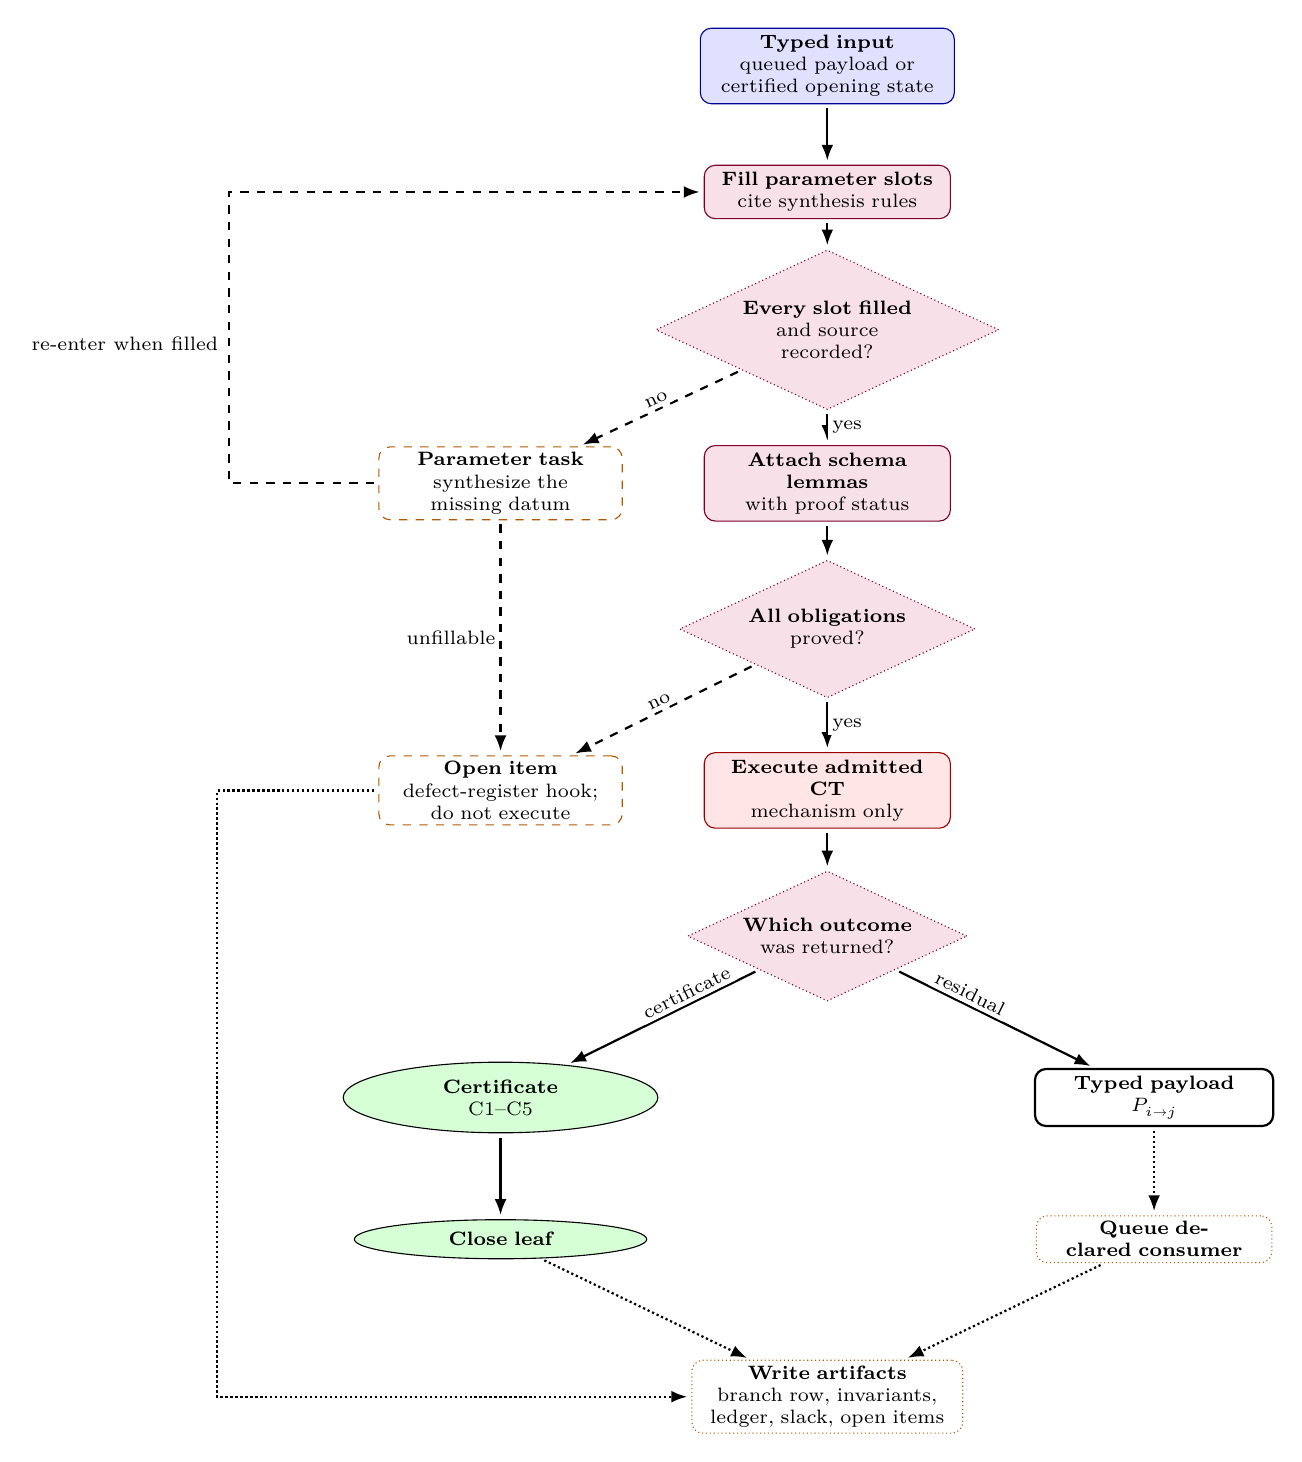
\begin{tikzpicture}[
x=1cm,
y=1cm,
every node/.style={font=\scriptsize}
]
\node[bcwide,bcdefinition,text width=3.05cm,minimum width=3.05cm]
  (payload) at (0,0) {\textbf{Typed input}\\queued payload or\\certified opening state};
\node[bcbox,bclemma,text width=2.95cm,minimum width=2.95cm]
  (params) at (0,-1.60) {\textbf{Fill parameter slots}\\cite synthesis rules};
\node[bcdec,bcaudit,text width=2.55cm,minimum width=3.25cm]
  (slotcheck) at (0,-3.35) {\textbf{Every slot filled}\\and source recorded?};
\node[bcroute,bcrouteneutral,bcdesign,text width=2.95cm,minimum width=2.95cm]
  (paramtask) at (-4.15,-5.30) {\textbf{Parameter task}\\synthesize the missing datum};
\node[bcbox,bclemma,text width=2.95cm,minimum width=2.95cm]
  (oblig) at (0,-5.30) {\textbf{Attach schema lemmas}\\with proof status};
\node[bcdec,bcaudit,text width=2.45cm,minimum width=3.15cm]
  (complete) at (0,-7.15) {\textbf{All obligations}\\proved?};
\node[bcroute,bcrouteneutral,bcdesign,text width=2.95cm,minimum width=2.95cm]
  (defect) at (-4.15,-9.20) {\textbf{Open item}\\defect-register hook; do not execute};
\node[bcbox,bctheorem,text width=2.95cm,minimum width=2.95cm]
  (execute) at (0,-9.20) {\textbf{Execute admitted}\\\textbf{CT}\\mechanism only};
\node[bcdec,bcaudit,text width=2.35cm,minimum width=3.05cm]
  (outcome) at (0,-11.05) {\textbf{Which outcome}\\was returned?};
\node[bcclosed,text width=2.65cm,minimum width=2.65cm]
  (cert) at (-4.15,-13.10) {\textbf{Certificate}\\C1--C5};
\node[bcbox,bcpayload,text width=2.85cm,minimum width=2.85cm]
  (outpayload) at (4.15,-13.10) {\textbf{Typed payload}\\\(P_{i\to j}\)};
\node[bcclosed,text width=2.45cm,minimum width=2.45cm]
  (halt) at (-4.15,-14.90) {\textbf{Close leaf}};
\node[bcroute,bcrouteneutral,bcoutputroute,text width=2.85cm,minimum width=2.85cm]
  (queue) at (4.15,-14.90) {\textbf{Queue declared consumer}};
\node[bcroute,bcrouteneutral,bcoutputroute,text width=3.30cm,minimum width=3.30cm]
  (artifacts) at (0,-16.90) {\textbf{Write artifacts}\\branch row, invariants, ledger, slack, open items};
\draw[bcarr] (payload)--(params);
\draw[bcarr] (params)--(slotcheck);
\draw[bcrecoverarr] (slotcheck)--node[bclabel,above,sloped]{no}(paramtask);
\draw[bcarr] (slotcheck)--node[bclabel,right]{yes}(oblig);
\draw[bcrecoverarr] (paramtask.west) -- ++(-1.90,0) |- node[bclabel,left,pos=0.24,xshift=-2pt]{re-enter when filled} (params.west);
\draw[bcrecoverarr] (paramtask)--node[bclabel,left]{unfillable}(defect);
\draw[bcarr] (oblig)--(complete);
\draw[bcrecoverarr] (complete)--node[bclabel,above,sloped]{no}(defect);
\draw[bcarr] (complete)--node[bclabel,right]{yes}(execute);
\draw[bcarr] (execute)--(outcome);
\draw[bcarr] (outcome)--node[bclabel,above,sloped,pos=0.35]{certificate}(cert);
\draw[bcarr] (outcome)--node[bclabel,above,sloped,pos=0.35]{residual}(outpayload);
\draw[bcarr] (cert)--(halt);
\draw[bchandoff] (outpayload)--(queue);
\draw[bchandoff] (halt)--(artifacts);
\draw[bchandoff] (queue)--(artifacts);
\draw[bchandoff] (defect.west) -- ++(-2.05,0) |- (artifacts.west);
\end{tikzpicture}%
}
\caption[Strategy worksheet flow]{Strategy worksheet flow.  Slot coverage and obligation completeness are separate pre-execution checks.  Only a complete worksheet crosses the mechanism boundary; the returned outcome is then classified as a certificate or typed payload, while pending obligations stop at a defect-register item.}
\label{fig:strategy-worksheet-flow}
\end{figure}

A new tactic entry is warranted at level-3 repair when a residual
survives admission, no listed CT consumes it, and it is expressible in
the current data language. Assign the next CT identifier and update the
frozen-library range declaration. Draft the complete tactic entry,
verify that every non-certificate output lands on an existing or newly
added trigger, and update the master CT ledger, signature and obligation
matrices, parameter-slot mapping, index card, payload table, and routing
graphs. Add a toy or [EG] instantiation, apply the level-3 exit test, and
close the defect-register item only if that test passes. A level-4 repair
first extends the data language, then applies the same registration and
exit tests to the new tactic family.


\section{Assurance}\label{part-iv-assurance}

\secref{part-iv-assurance} is the verification layer around the motivation, mechanism, and
policy layers. It contains the
certificate and branch-table discipline, the global checklists,
proof-engineering artifacts, constant interlocks, failure semantics, the
defect register, LLM operationalization, portability, and the scope
limitations. It does not choose tactics and does not execute tactics; it
audits that each admitted invocation, policy decision, and routed
payload has been recorded.

\begingroup
\small
\setlength{\tabcolsep}{2pt}
\begin{longtable}[]{@{}
  >{\raggedright\arraybackslash}p{0.22\linewidth}
  >{\raggedright\arraybackslash}p{0.56\linewidth}
  >{\raggedright\arraybackslash}p{0.14\linewidth}@{}}
\toprule\noalign{}
Assurance artifact & Verification role & Source \\
\midrule\noalign{}
\endhead
\bottomrule\noalign{}
\endlastfoot
Branch table & One row per terminal branch or named residual; every row points to a worksheet or certificate. & \secref{the-branch-table} \\
Worksheet list & One row per CT invocation, including pending obligations and emitted payloads. & \secref{filling-the-templates} \\
Dependency graph and table & Nodes, dichotomies, and lemma clusters; every leaf named. & \secref{proof-engineering-artifacts} \\
Invariant register and reverse index & Standing hypotheses and their consumers; supports blast-radius computation. & \secref{proof-engineering-artifacts} \\
Slack and constant interlock & Numerical constants, inequalities, margins, and finite computations. & \secref{constant-interlock-and-computational-certificates} \\
Resilience register & Reduction theorem that survives each hypothetical closure failure. & \secref{redundant-closures-and-graceful-degradation} \\
Defect register & Structured record of discovered execution errors, design repairs, and pattern-level additions. & \secref{the-defect-register-recording-discovered-failures} \\
\end{longtable}
\endgroup

\subsection{Decoupling conformance checks}\label{decoupling-verification-checks}

The following table defines release conformance for the mechanism/policy
separation. M1--M6 and H3--H4 are normative release checks. H1--H2 are
usability goals, not completeness theorems.

\begingroup
\small
\setlength{\tabcolsep}{2pt}
\begin{longtable}[]{@{}
  >{\raggedright\arraybackslash}p{0.08\linewidth}
  >{\raggedright\arraybackslash}p{0.34\linewidth}
  >{\raggedright\arraybackslash}p{0.50\linewidth}@{}}
\toprule\noalign{}
ID & Check & Passing condition \\
\midrule\noalign{}
\endhead
\bottomrule\noalign{}
\endlastfoot
M1 & Policy purity of entries & The CT ledger in \secref{part-ii-the-tactic-library} and entries contain no selection advice except the quoted forbidden-word list in the decoupling contract. \\
M2 & Mechanism purity of strategy & \secref{part-iii-the-strategy-manual} describes admission, selection, synthesis, and composition; it does not restate CT-internal procedures except in the worksheet template. \\
M3 & Slot--rule bijection & Each parameter family in the CT ledger is covered by a rule in \secref{parameter-synthesis}; each rule names its consuming tactics. \\
M4 & Worksheet coverage & Each \appref{appendix-c.-a-small-worked-instantiation} trace row is either a reject row or has a worksheet-consistent tuple; CT2-1 and CT9-1 are fully displayed. \\
M5 & Failure-classification compliance & Each scope-obstruction entry is a nonexistence statement; execution errors appear as audit hooks or defect-register rejects; design failures appear as routed payloads. \\
M6 & Graph regeneration & The interlock graph is generated by the union of intended-output fields, and the repair graph by the union of recovery-output fields; the success sinks are exactly C1--C5, with C3 present. \\
H1 & Mechanism usability goal & A reader can apply a CT entry from the vocabulary of \secref{part-ii-the-tactic-library} plus the CT entry itself without consulting \secref{part-iii-the-strategy-manual}. \\
H2 & Policy usability goal & A reader can decide what to do next from \secref{part-iii-the-strategy-manual} plus \appref{appendix-d.-quick-reference-card}, using only Block 1 and scheduler data from \secref{part-ii-the-tactic-library}. \\
H3 & Index-card coverage & \appref{appendix-d.-quick-reference-card} lists ID, name, tier, cost class, trigger, certificates, and residual edges for every CT. \\
H4 & Worksheet auditability & The displayed worksheets identify input payloads, parameters, obligations, outcome, artifacts, and open items. \\
\end{longtable}
\endgroup

These checks are manuscript invariants. A contributor adding a CT,
payload edge, worksheet field, or policy rule must use a declared
extension namespace, record the library version and compatibility, and
update every registry or derived view whose invariant changes.

\subsection{LLM and formalization bridge}\label{llm-and-formalization-bridge}

The formalization bridge of \secref{the-formalization-bridge}
extends to these artifacts as follows.

\begingroup
\small
\setlength{\tabcolsep}{2pt}
\begin{longtable}[]{@{}
  >{\raggedright\arraybackslash}p{0.24\linewidth}
  >{\raggedright\arraybackslash}p{0.34\linewidth}
  >{\raggedright\arraybackslash}p{0.34\linewidth}@{}}
\toprule\noalign{}
Artifact & Formal counterpart & AI-facing role \\
\midrule\noalign{}
\endhead
\bottomrule\noalign{}
\endlastfoot
Instantiation worksheet & One proof-script step with named subgoals for each schema obligation. & Converts generated prose into statused obligations and defect hooks. \\
Selection policy & Tactic orchestration rule set, in the style of ordered tactic hints or an \texttt{aesop}-style rule base. & Restricts model freedom to admission, selection, and parameter synthesis. \\
Payload queue & Typed goal stack or worklist of unconsumed intermediate terms. & Prevents orphan residuals by forcing every emitted payload to be consumed or recorded. \\
\end{longtable}
\endgroup

\subsection{Constant interlock and computational
certificates}\label{constant-interlock-and-computational-certificates}

In a quantitative branch system, the numerical constants are
load-bearing interfaces. The discipline has four parts. Every constant
is \emph{named}, displayed to full stated precision, and
\emph{established at a cited location}. Every finite enumeration behind
a constant is reproduced by \emph{published code}, so that the leaf is
machine-checkable. The \emph{interlock} records which inequality each
constant must clear, and by what margin. The slack table identifies the
binding constraint, namely the inequality with the least slack. A change
to any constant can be impact-checked through the artifacts of \secref{proof-engineering-artifacts}. The proof records every constant at the precision used, so a constant used at higher precision than it was
established, and unrecorded slack consumption --- two branches
independently ``using up'' the same margin.



\subsection{Proof-engineering
artifacts}\label{proof-engineering-artifacts}

A branch system beyond a handful of branches requires explicit audit
artifacts, each of which mechanizes one clause of the audit checklist
(\secref{audit-checklist-for-branch-design}):

\begin{itemize}
\tightlist
\item
  a \textbf{dependency graph} with uniquely numbered nodes ---
  assertions, dichotomies, and terminal leaves --- in which every
  dichotomy has both edges resolved and every leaf is a named closure or
  a named residual;
\item
  a \textbf{dependency table} mapping node ranges to the lemma clusters
  that implement them;
\item
  an \textbf{invariant register}: the numbered list of standing
  invariants (the accumulated branch-state facts), grouped by the stage
  at which each is established;
\item
  \textbf{per-lemma requirement rows}: for each lemma, the invariants
  and prior results it consumes, so that every consumed hypothesis is
  recorded;
\item
  a \textbf{reverse index} from each invariant to every lemma that
  consumes it --- the impact-analysis table that answers ``if this
  invariant weakens, what breaks?'' by lookup.
\end{itemize}

These artifacts are the audit scaffold of the closure claim,
and they support the AI-assisted workflow of \secref{design-rationale-scaffolding-for-llm-assisted-proof-development} at scale: every
one of the four failure modes leaves a visible trace in at least one
artifact.



\subsection{Redundant closures and graceful
degradation}\label{redundant-closures-and-graceful-degradation}

Many long proofs behave conjunctively: the theorem is represented as the
conjunction of its closing lemmas, so a false or incomplete lemma can
create an unlocalized gap whose exact extent is difficult to determine
without re-auditing the argument. The branch-closure architecture
assigns a different semantics to failure. The central property is the
\textbf{degradation invariant}:

\begin{quote}
At every stage of construction, audit, or repair, the document proves a
true reduction theorem. A lemma failure changes \emph{which} reduction
theorem is proved; it never changes \emph{whether} one is proved.
\end{quote}

\paragraph{The failure-to-reduction
transformation}\label{the-failure-to-reduction-transformation}

Suppose a lemma \(L\) closes branch \(B\), whose residual class is
\(\mathcal C_B\), and suppose \(L\) is later found to be false or
incomplete. Because the method forbids unnamed residuals (\secref{closure-criteria-and-the-branch-table}),
\(\mathcal C_B\) already exists as a defined object. It carries exact
data: the branch state under which it arose, the baseline hypotheses,
minimality, every standing invariant of the load path, the formal
absence of all other exits, and the relevant minimality, carrier, and
type data. Assume here that the branch partition is exhaustive, every
other branch closure and every ancestor of the statement remain sound,
and the reverse dependency data are complete. Under those assumptions,
the surviving statement is:

\[
\begin{gathered}
\textbf{Reduction theorem.}\\
\text{The main theorem holds unless a counterexample lies in } \mathcal C_B.
\end{gathered}
\]

The residual \(\mathcal C_B\) inherits every invariant that the reverse
index shows to be established upstream of \(L\). This transformation is
a consequence of the closure discipline: a residual that was named,
typed, and routed while the proof was presented as complete is also a
residual that can stand alone when a closure is retracted. The failed
closure is replaced by a weaker theorem with an explicit exceptional
class.

\paragraph{Declared dependency closure}\label{bounded-blast-radius}

The damage caused by a failure is computable from the audit artifacts.
The invariant register records which invariants \(L\) establishes; the
reverse index maps each such invariant to the lemmas consuming it; the
dependency graph gives the transitive closure. This downstream set is
the \textbf{declared dependency closure}, also called the blast radius,
of \(L\).

The architecture makes this set explicit, but does not imply that it is
small. Branch states preserve upstream information along a load path;
certificate dependencies are explicitly scoped rather than uniformly
bounded-local; and typed handoffs (\secref{typed-handoffs-between-branches}) give inter-branch
dependencies declared payloads and edges. Terms such as ``small'' or
``bounded'' require a measured case-study result.

\paragraph{Redundant layers and slack
absorption}\label{redundant-layers-and-slack-absorption}

Two buffers may absorb a failure before it re-opens a branch. The first
is \textbf{redundancy}: where the architecture provides arithmetically
distinct closures for the same contradiction --- an entropy cap, a rank
squeeze, and a charge collision, for example --- a branch re-opens only
when every layer supporting that closure fails. A numerical repair in
one layer preserves the formal content of the other layers.

The second buffer is \textbf{slack}. When the failure is quantitative,
for instance because a constant is established with less margin than
expected, the slack table (\secref{budget-separation-and-slack-accounting}) determines whether recorded
unspent margin covers the loss. In that case the repair is a
re-computation rather than a redesign. The constant interlock classifies
each quantitative failure as slack-absorbable, transferable to a
redundant layer, or branch-reopening.

\paragraph{The repair protocol}\label{the-repair-protocol}

A re-opened branch is repaired with the same template that built the
proof. Repair begins from the surviving verified ancestor state computed
by dependency analysis: only upstream invariants independent of the
failed result remain available, while the residual records where the
difficulty lies. Repair proceeds through four levels.

Before choosing a level, open a defect-register row for the failed
closure. Record the failed dependency-graph node and, when applicable,
the schema, the
residual class \(\mathcal C_B\), the surviving reduction theorem, the
upstream invariants inherited by \(\mathcal C_B\), and the blast radius
computed from the reverse index. Then classify the defect as an
execution error \((E)\), a repairable design failure \((D)\), or a
candidate scope obstruction. An omitted or incorrectly discharged
finite-computation obligation is an execution error and starts at level
1. A schema or structural execution error starts at level 2. A verified
numerical failure that emits a legal typed residual naming its binding
term is a design failure and also starts at level 2. A legal design
residual reaches level 3 only when its declared consumers and every
existing pattern composition fail to close it or advance its declared
measure. A routing execution error requiring a new interface triggers a
level-3 interface review, but is reclassified as \((D)\) only after the
payload-table entry and unique consumer are declared, the producer's
routing obligation is discharged, and the consumer's trigger obligation is
recorded for discharge at admission. A candidate scope obstruction
reaches level 4 and is classified as an
intrinsic scope obstruction \((S)\) only after the audit proves that the
residual is not expressible in the current proof language. Repairs are
attempted at the lowest applicable level and escalate only when that
level's exit test fails.

\begin{enumerate}
\def\labelenumi{\arabic{enumi}.}
\item
  \textbf{Numerical repair.} This level applies when the definitions,
  branch partition, payload routes, and lemma statements remain valid
  and only a finite computation or quantitative value has failed.

  \emph{Audit.} Freeze the branch state and trace every affected number
  through the constant interlock, slack table, and reverse index. Check
  the value at the precision at which it is consumed, rather than at a
  rounded display precision. The audit distinguishes four cases.

  \begin{itemize}
  \item
    \textbf{Finite enumeration or computational certificate.} Reproduce
    the computation from its declared input domain. Verify the pruning
    rules, coverage of every terminal case, exact arithmetic, and the
    published certificate or checksum. Correct a code error, stale
    output, or transcription error and regenerate every dependent
    constant. The defect row records the checker identity and version,
    exact command, trusted inputs, and verification status. A correct
    computation with an incorrect domain or missing case is a structural
    defect and moves to level 2.
  \item
    \textbf{Constant or precision.} Re-derive the constant from the
    cited inequalities and compare its established precision with every
    use listed in the reverse index. Replace the value consistently in
    the constant interlock and all consuming inequalities. If the
    derivation itself uses a false hypothesis, incompatible currency, or
    omitted boundary term, move to level 2.
  \item
    \textbf{Rate interval.} Recompute
    \(\rho_{\mathrm{sup}}\) and \(\rho_{\mathrm{dem}}\), including the
    strictness of both endpoints and every parameter on which they
    depend. When the interval remains nonempty, choose and record a new
    rate in its interior as in \secref{computing-rates-backwards}. An
    empty interval identifies a binding supply or demand term and moves
    to level 2.
  \item
    \textbf{Slack allocation.} List every consumer of the affected
    margin and compare the list with the slack table. Spend only slack
    recorded as unassigned, or transfer the closure to an
    arithmetically independent redundant layer. A margin already spent
    by another branch, or two nominally redundant closures drawing on
    the same margin, is a level-2 accounting defect.
  \end{itemize}

  \emph{Exit test.} Reverify the finite certificates and every affected
  inequality. Each must hold with its new recorded margin. Update the
  numerical fields in the constant interlock, slack table, invariant
  records, and dependent inequalities; the branch partition, lemma
  statements, payload signatures, and graph topology remain unchanged.
  Otherwise the repair escalates to level 2.
\item
  \textbf{Structural repair inside the pattern library.} Treat
  \(\mathcal C_B\) as a fresh residual and apply
  \secref{choosing-invariants-and-building-budgets} using the recorded workflow and existing
  tactic vocabulary. The repair may change invariants, labels, budgets,
  worksheets, or routes, but it uses only the existing proof language
  and closure taxonomy.

  \emph{Audit and repair by failure type.}

  \begin{itemize}
  \item
    \textbf{Failed hypothesis or stale branch state.} Use the
    per-lemma requirement row to find the first unavailable invariant,
    and use the reverse index to locate every consumer. Check
    measurability, ladder position, and whether the invariant was derived
    before it was used. Derive it from an earlier resource, weaken or
    restage the consuming estimate, and separately close the invariant's
    failure branch by the both-sides test.
  \item
    \textbf{Ledger or budget defect.} Audit the canonical assignment rule,
    payer uniqueness, capacities, additivity, boundary corrections,
    moves \(\times\) budgets table, and separation of currencies.
    Repair a missing compensating term or boundary correction; localize
    the deficit; split competing demands into recorded fractions; or use
    an existing tier, peel, or aggregate closure. A new tier is governed
    by \secref{tiered-charging-scheme-failure-as-a-demand}, a peel by
    \secref{peeling-loops-closure-by-well-founded-recursion}, and an
    aggregate bound by
    \secref{aggregate-closure-mass-bounds-on-residual-classes}.
  \item
    \textbf{Label or type defect.} Check that the label alphabet is
    finite, measurable from the branch state, and fine enough to support
    every downstream dichotomy. Check that the context generator covers
    every permitted attachment and that exact-type comparisons use
    literal equality. Repair by refining the finite label, enlarging the
    certified context generator, adjusting the threshold, or computing
    a sharper exact type. Label refinement follows
    \secref{the-default-refinement}.
  \item
    \textbf{Routing or schema defect.} Compare the worksheet input and
    output with the tactic signature, routing, trigger, and the declared
    consumer's trigger. Discharge a missing schema obligation when the
    required datum is already present. When the route is already
    declared, construct the payload exactly as declared and verify that
    the producer output field, payload-table row, and consumer signature
    agree. Reverify the producer's routing certificate, and record and
    verify the consumer's trigger obligation for discharge when that
    consumer is admitted; then regenerate the affected interlock and
    repair graphs. An untyped output, an output with no
    unique declared consumer, or a repair requiring a new producer
    field, payload-table entry, or consumer signature is an execution
    reject. Record it without emitting or queuing it, and send it to the
    level-3 interface review.
  \item
    \textbf{Progress or termination defect.} Verify S-Meas on every
    cyclic or recursive non-closing transition, and verify S-Rest when a
    transition restores branch state. An acyclic handoff requires
    routing and trigger but need not decrease a measure. Repair a
    stationary cycle by splitting it at the next routing principle,
    refining its descriptor, or applying the existing peel, tier, or
    well-founded measure. A cycle with no decreasing measure cannot be
    admitted.
  \item
    \textbf{Black-box interface defect.} Compare the registered
    hypotheses and conclusion with the exact cited statement and with
    each consuming requirement row. Weaken the interface to the cited
    theorem and weaken or restage every consumer whose requirement
    exceeded it. Alternatively, supply a missing hypothesis from the
    branch state, branch on that hypothesis and close its failure side,
    or route the missing-hypothesis obligation to a declared producer. A
    stronger unconditional statement is not a repair inside the existing
    library.
  \end{itemize}

  \emph{Exit test.} Re-run admission and selection, the invariant and
  budget checklists, the moves \(\times\) budgets audit, affected
  worksheets, and routing and trigger for each regenerated route. Every
  leaf must return C1--C5 or a typed payload to an existing consumer.
  Keep at level 2 any execution error correctable without an interface
  change. Send an interface-changing routing reject to level-3 review;
  it remains \((E)\) until its payload-table row, unique consumer,
  producer's routing certificate, and consumer's trigger obligation are
  recorded. Move a legal, expressible residual unmatched by the taxonomy
  to level 3. Record an inexpressible datum as a candidate scope
  obstruction and send it to the level-4 audit.
\item
  \textbf{Pattern-level repair.} This level applies when
  \(\mathcal C_B\) is expressible using existing descriptors and schema
  obligations, but no pattern in \secref{the-branch-taxonomy} or
  \secref{advanced-closure-patterns} closes it.

  \emph{Audit.} Normalize the residual by recording its descriptor
  inventory, input payload, inherited invariants, live exits, available
  certificates, current typed consumers, and progress measure. Check the
  existing taxonomy after permissible relabelling, sequencing, typed
  handoff, and black-box composition. First distinguish legal recurrence
  from an execution error: a return with unchanged state and no decrease
  on a required measure is rejected, whereas a legally decreasing
  recurrence may indicate a missing pattern. The following signatures
  support a pattern-level repair: the same normalized routing defect
  recurring after the level-2 audit; a legal typed residual repeatedly
  returned by its declared consumers without closure; the same defect class
  recurring in two or more branches; a residual that repeatedly stops
  shrinking; a branch whose cases share a new routing principle; or a
  closure assembled from existing tactics but absent from the pattern
  library.

  \emph{Repair by failure type.} Merge branches whose failure sides have
  the same route, and split a nonshrinking branch at the first routing
  principle that distinguishes its outcomes. Repair a routing defect
  requiring a new interface by declaring one abstract producer--consumer
  contract. A legal residual returned without closure requires a pattern
  with an explicit decreasing measure. When a closure is assembled from existing tactics,
  record its sequencing and typed handoffs as a combinator and add its
  reusable closure statement as an advanced pattern. For every recurrent
  residual, state one abstract pattern whose input is
  the normalized residual signature. The pattern must declare its
  trigger, inherited data, closure certificate, non-closing typed outputs
  and their consumers, scope obstruction, well-founded measure, and
  artifact writes. Add the pattern to
  \secref{advanced-closure-patterns}, instantiate it on \(\mathcal C_B\),
  update every affected producer output field, payload-table entry, and
  consumer signature. If the repair adds a tactic, assign the next CT
  identifier and update the frozen-library range declaration; register a
  complete entry with its signature, trigger, parameters, procedure,
  obligations, certificates, outputs, audit hooks, and scope obstruction,
  and update the master CT ledger, signature and obligation matrices,
  parameter-slot mapping, and index card. Discharge the producer's
  routing obligation, and record and verify the consumer's trigger
  obligation for discharge when that consumer is admitted. Then
  regenerate the dependency, interlock, and repair graphs together with
  the branch table and worksheets. Once the payload-table entry, unique
  consumer, and routing certificate are present, reclassify the routing
  reject from \((E)\) to \((D)\) and admit its payload; the consumer
  discharges trigger when it accepts that payload.

  \emph{Exit test.} Every outcome of the new pattern must close at
  C1--C5 or enter an existing consumer through a typed payload, and every
  loop must decrease the declared measure. If the pattern cannot be
  stated using the current descriptor types, the obstruction moves to
  level 4.
\item
  \textbf{Language extension.} This level applies to a candidate scope
  obstruction: the needed object may not be expressible by the current
  local tests, bounded interfaces, finite context generators, finite
  labels, additive budgets, or measurable loads.

  \emph{Audit.} First prove nonexpressibility in the current language by
  identifying the missing datum and showing that no existing descriptor
  records it. A missing lemma or untried pattern is not a language
  obstruction. Once nonexpressibility is established, classify the
  defect as an intrinsic scope obstruction \((S)\). Then determine
  whether the proposed datum admits a finitely encoded descriptor
  hierarchy, canonical extraction from the branch state,
  compatibility with the declared gluing or decomposition operations,
  finite certificate semantics, the applicable S-Pers and equivalence
  obligations, and a well-founded progress measure. These conditions
  decide whether the obstruction is repairable at level 4 or terminal.
  For cut and energy residuals, the witnessed set or Rayleigh function
  may be global, but its routed descriptor record must be finitely
  encoded: for example, by volume, boundary mass, conductance scale, side
  profiles, and recursive obligations.

  \emph{Repair by failure type.} For a missing local test or bounded
  interface, declare the test family, attachment data, and finite context
  generator. For a missing label or type, declare the finite label or
  finitely encoded descriptor record and its equality or refinement
  rule. For a missing budget or load,
  declare its currency, additivity domain, canonical extraction, and
  measurable progress quantity. Every extension must specify its
  descriptor type and payload format; auxiliary finite certificate data;
  the existing terminal class among C1--C5 that validates each closing
  leaf; schema obligations; parameter-synthesis rules; producer and
  consumer tactics; and non-closing routes back to the existing interlock
  graph. Assign each new tactic the next CT identifier and update the
  frozen-library range declaration. Register every new producer or
  consumer as a complete CT entry with its signature, trigger, parameters,
  procedure,
  obligations, certificates, outputs, audit hooks, and scope obstruction.
  Update the master CT ledger, signature and obligation matrices,
  parameter-slot mapping, index card, tactic output fields, payload
  table, consumer signatures, branch table, worksheet fields, assurance
  checks, quick-reference card, and limitations.
  Discharge each producer's routing obligation, and record and verify each consumer's
  trigger obligation for discharge at admission; then regenerate the
  interlock and repair graphs before using the new language.

  \emph{Exit test.} Re-run the level-2 closure procedure in the extended
  language. The extension is admitted only when every output closes or
  routes, every cyclic or recursive route decreases the declared measure,
  and S-Rest holds whenever a route restores branch state. If no
  finitely encoded descriptor hierarchy equipped with a well-founded
  measure exists, record a terminal scope obstruction and retain the
  surviving reduction theorem. Its defect-register row remains open with disposition
  \texttt{terminal-S}; it is not closed while that theorem remains
  conditional. Here terminal means terminal for the current language
  only; it is neither a closed proof leaf nor evidence of leaf-totality.
\end{enumerate}

Every attempted repair updates the defect-register row before the proof
is rerun. For each attempt, append its audit evidence, repair level,
pre- and post-repair classification and disposition, exact edit,
exit-test result, post-repair dependency set, and reduction theorem
currently in force. The blast radius at discovery remains
immutable. A defect is closed only after the applicable exit test
passes; until then the row remains open and the current residual class,
initially \(\mathcal C_B\), remains among the exceptional classes named
by the recorded reduction theorem.

At levels 3 and 4, the typed residual becomes either a reusable closure
pattern or vocabulary in which later patterns can be stated.

\paragraph{The resilience register and the reduction
lattice}\label{the-resilience-register-and-the-reduction-lattice}

The \textbf{resilience register} makes the degradation invariant
auditable. It has one row per intermediate branch, recording the branch
state, the residual class published if its closure fails, the blast
radius computed from the reverse index, the surviving reduction theorem,
and the anticipated repair level. Maintaining the register is
inexpensive because each column is read from artifacts already required
by \secref{proof-engineering-artifacts}.

The register also gives the global structure of a proof in progress. The
proved reduction theorems form a lattice ordered by inclusion of
excluded residual classes. Verifying a closure moves the proof upward in
the lattice; retracting a closure moves it downward by one computable
step; the unconditional theorem is the top element. A referee who has
checked \(k\) of \(N\) branches has established the reduction theorem
corresponding to those \(k\) closures, unconditionally. The same
containment governs the AI-assisted workflow of \secref{design-rationale-scaffolding-for-llm-assisted-proof-development}: a fabricated
or incomplete step affects one node, is detected by the artifacts, and
lowers the lattice position by a specified step.

\textbf{Register integrity.} Graceful degradation is a property of the
maintained architecture. A stale reverse index reports a false blast
radius, and an undeclared handoff introduces an untracked dependency.
Both errors convert a mesh of reductions into a chain of implicit
assumptions. The degradation invariant also requires exact residual
statements: a vague claim with no corresponding element in the reduction
lattice is not a surviving reduction theorem.
Finally, redundant layers must be arithmetically independent. Two
closures that consume the same slack margin or the same invariant form
one layer with two names; the slack table and reverse index are the
instruments that detect this collapse.



\subsection{The defect register: recording discovered
failures}\label{the-defect-register-recording-discovered-failures}

The resilience register of \secref{the-resilience-register-and-the-reduction-lattice} records what survives under
hypothetical failures. Its temporal complement is the \textbf{defect
register}: the structured record of every defect actually discovered
during construction or audit, together with the way the document
absorbed it. The resilience register is predictive; the defect register
is evidentiary. It turns the assertion that a manuscript has been
audited into a checkable object.

Each entry has a fixed schema.

\begin{enumerate}
\def\labelenumi{\arabic{enumi}.}
\tightlist
\item
  \textbf{Identifier.} A stable ID, with defects grouped into lettered
  families by kind.
\item
  \textbf{Location.} The affected dependency-graph node or nodes and the
  affected lemma or lemmas. Nodes are used rather than page numbers,
  since pages drift and nodes are stable.
\item
  \textbf{Classification.} The formal class \((E)\), \((D)\), or
  \((S)\), or the provisional status ``candidate scope obstruction,''
  together with the concrete subtype and
  the failure mode of
  \secref{design-rationale-scaffolding-for-llm-assisted-proof-development}
  or checklist item of
  \secrange{audit-checklist-for-branch-design}{choosing-invariants-and-building-budgets}
  that the defect violates. Typical subtypes include quantifier-scope
  collapse, phantom ledger entry, double-charged token, currency mismatch
  between accounts, and unrecorded exit dependence. For tactic
  invocations, the classification also records the CT instance and
  schema name, for example CT7-3/equivalence or CT12-1/S-Rest.
\item
  \textbf{Residual and surviving theorem.} The current residual class,
  initially \(\mathcal C_B\), its inherited upstream invariants, and the
  exact reduction theorem that remains in force while the defect is open.
\item
  \textbf{Audit evidence.} The failed obligation, computation,
  dependency, or nonexpressibility statement supporting the
  classification, together with the residual's normalized failure
  signature when level 3 or 4 is under consideration.
\item
  \textbf{Blast radius at discovery.} The downstream set computed from
  the reverse index as in \secref{bounded-blast-radius}, recorded before the repair is
  made and never overwritten by later repairs.
\item
  \textbf{Repair history.} An append-only sequence with one entry per
  attempt. Each entry records the repair level, pre- and post-repair
  classification and disposition, exact edit (including any invariant
  added, weakened, or re-staged), exit-test result, resulting downstream
  dependency set, descendant residual, and reduction theorem then in
  force. A later attempt never overwrites an earlier one or the blast
  radius at discovery.
\item
  \textbf{Status.} Open or closed. An open defect records the reduction
  theorem currently in force, which is the degradation invariant applied
  to the audit history. A terminal scope obstruction remains open with
  disposition \texttt{terminal-S}; it is not a closed defect.
\end{enumerate}

Three disciplines make the register load-bearing. First, every repair
cites its defect ID, so the proof's edit history is navigable by defect
rather than by line number. Second, open defects are explicit entries: a
register listing only closed defects is incomplete, while a complete
register states the current lattice position of \secref{the-resilience-register-and-the-reduction-lattice}. Third,
recurrence triggers pattern or language review: two or more defects in
the same class signal that the pattern library is missing a closure
shape, or that the current vocabulary lacks the descriptor in which the
closure should be stated. The appropriate repair is then a new
\secref{advanced-closure-patterns} pattern or a level-4 language extension. In this
sense the defect register supplies empirical input to the method: it
records which repairs recur often enough to deserve names or new data
types.

The register also closes a loop with the AI-assisted workflow of \secref{design-rationale-scaffolding-for-llm-assisted-proof-development}. Each
defect classification names the failure mode that produced it, so the
register becomes a calibration record for machine assistance: it records
where the assistance failed and whether the proof artifacts caught the
failure at the intended layer.

\textbf{Scope-obstruction escalation rule.} Every non-closing branch is
classified before it is allowed to terminate. An execution error \((E)\)
means that a named obligation is unfilled or incorrectly discharged,
including a computational certificate; the register records the CT
instance, the schema or certificate, and the missing or invalid
derivation, and the repair is to discharge that obligation correctly. A
repairable design failure
\((D)\) means that the failed datum is a typed residual; the register
records the emitted payload and follows the corresponding output edge in
the interlock graph. An intrinsic scope obstruction \((S)\) means that
the needed bounded object is not expressible in the current proof
language: no local test family, no bounded interface, no finite context
generator, no finite label space, no additive budget, or no measurable
load. The defect register then decides whether the obstruction admits a
  finitely encoded proof-language extension and a well-founded progress
  measure. If it does, the repair is level 4; if it does not, the obstruction is
terminal and routes to the limitations section
\secref{the-scope-condition-locally-testable-targets}. Inside an
admissible proof language, the framework has unfilled or incorrectly
discharged obligations, legal routed design residuals, and routing
execution rejects, not terminal scope obstructions.

\textbf{Register-location invariant.} A register keyed to prose
locations decays with every revision; node-based locations are stable. A
register maintained only at release time records the repairs but not the
blast radii at discovery, which is the evidence needed to validate the
bounded-blast-radius claim of \secref{bounded-blast-radius}.



\subsection{Repair taxonomy and common failure shapes}\label{repair-taxonomy-and-common-failure-shapes}

The repair protocol above separates failures by the contract that breaks.
Every failure in this manual has the same core shape: a declared resource
is missing, stale, misrouted, or not expressible in the current language.
The difference is which declaration fails first. Some failures are local
computational mistakes; some are structural mismatches inside the current
pattern library; some are legal residuals that need a different pattern;
and some exceed the current language entirely.

\begin{longtable}[]{@{}
  >{\raggedright\arraybackslash}p{0.16\linewidth}
  >{\raggedright\arraybackslash}p{0.24\linewidth}
  >{\raggedright\arraybackslash}p{0.21\linewidth}
  >{\raggedright\arraybackslash}p{0.29\linewidth}@{}}
\toprule\noalign{}
Failure family & What breaks & First repair move & Prevention rule \\
\midrule\noalign{}
\endhead
\bottomrule\noalign{}
\endlastfoot
Execution error \((E)\), level 1 & A finite computation, constant, precision, or certificate is wrong or stale. & Recompute at the consumed precision, refresh all dependent values, and update the constant interlock, slack table, or certificate row. & Record the source computation, the exact precision, and every consumer before the value is used. \\
Structural execution error \((E)\), level 2 & A hypothesis, branch state, route, or schema obligation is missing, outdated, or inconsistent. & Restage the missing invariant, repair the route table, or discharge the schema against the current branch state. & Keep the dependency graph and reverse index current, and verify routing and trigger at every handoff. \\
Repairable design failure \((D)\), level 2 & A legal typed residual has appeared, but the current tactic library has not yet consumed it. & Send the residual to an existing consumer by a declared payload, or move the residual to CT4, CT10, CT13, CT14, CT15, or CT17 as appropriate. & Declare the output field, payload tuple, and unique consumer at the moment the residual is introduced. \\
Pattern gap \((D)\), level 3 & The residual is legal and expressible, but no existing pattern closes it. & Abstract the recurring residual into a reusable pattern, then register the new combinator or CT entry and regenerate the dependency graphs. & Watch for repeated residual signatures, repeated nondecrease, or repeated routing defects across branches. \\
Language gap \((S)\), level 4 & The needed object cannot be expressed with the current finite interfaces, labels, or descriptors. & Extend the language with a finitely encoded descriptor hierarchy and a well-founded progress measure, or record the obstruction as terminal. & Check expressibility before proof search begins: if the needed datum has no declared descriptor, no local repair will finish the job. \\
\end{longtable}

Three common invariants run through the table. First, the defect register is
append-only: the blast radius at discovery is part of the evidence, not a
detail to be reconstructed later. Second, every repair is local to the
failure class: numerical repairs do not change the interface; structural
repairs do not change the meaning of the theorem; pattern repairs add a
new reusable shape; language repairs add a new descriptor language. Third,
prevention is mostly bookkeeping discipline. Keep the declared consumer
fixed, keep the payload signature explicit, record the exact measure or
precision at which the object is consumed, and rerun the relevant audit
checks before the object is admitted downstream.

For framework design, the useful summary is short. If the defect is
numerical, tighten the arithmetic and update dependent constants. If the
defect is structural, restore the missing hypothesis or route. If the
defect repeats, factor it into a pattern. If the needed object is
inexpressible, the framework needs a language extension rather than a
local fix. That separation is what keeps the repair ladder finite and the
taxonomy reusable.

\subsection{Portability}\label{portability}

The method is designed for classes of objects in which there is a target
predicate; local modifications can be compared against outside contexts;
minimality yields a replacement principle; branch states admit finite
labellings; and global constraints are expressible as charging schemes.

Candidate domains include extremal graph theory,
Ramsey-type problems, colouring and list-colouring, forbidden-substructure
problems, minors and immersions, additive-combinatorial configurations,
matroid representability obstructions, and constraint satisfaction and
finite model theory. The portability claim is strongest in settings
where the comparison literature already has traction: local
reducibility, finite interfaces, representative replacement, and
charging/discharging all need local definitions compatible with the
target predicate
\citep{appel-haken-1977-discharging, robertson-etal-1997-four-colour, courcelle-1990-mso-graphs, courcelle-engelfriet-2012-graph-structure, bodlaender-etal-2009-meta-kernelization}.
This manual demonstrates the graph setting; each other domain requires
its own verified interfaces, types, replacement rules, and capacity
arguments.

One common base-language pipeline is:

\[
\begin{gathered}
\text{minimal counterexample}
\Rightarrow
\text{local tests}
\Rightarrow
\text{branch states}\\
\Rightarrow
\text{charging scheme}\\
\Rightarrow
\text{overloaded label class}
\Rightarrow
\text{bounded exchange}\\
\Rightarrow
\text{hit / defect / compression}.
\end{gathered}
\]

Direct target, minimality, and finite-exhaustion branches may bypass the
charging, overload, or exchange stages.

Equivalently,

\[
\boxed{
\begin{gathered}
\text{Every way of avoiding the target costs a scarce resource,}\\
\text{violates an accumulated exclusion,}\\
\text{or creates a repeatable local operation.}
\end{gathered}
}
\]

Scarce resources are charged by charging schemes, exclusions are spent
by branch-state dichotomies, and repeatable local operations are closed
by hit, defect, or compression. This is the core mechanism.

\subsection{Limitations}\label{limitations}

The method has a precise scope condition and a nontrivial cost. Both are
part of the framework. This section records where the machinery applies
and what it charges when it does.

\subsubsection{The scope condition: locally testable
targets}\label{the-scope-condition-locally-testable-targets}

The base tactic library consumes bounded-radius, bounded-interface data:
local tests, external types, finite labels, charging schemes, and the
exchange trichotomy. This gives the base proof-language scope condition.

\begin{quote}
\textbf{Base proof-language scope condition.} The target must admit a local test family
(\secref{target-predicate-and-local-tests}) whose bounded-interface types have finite Myhill--Nerode
index under gluing. In graph-sequence language, the target must be
visible to local Benjamini--Schramm data rather than only to a global
invariant.
\end{quote}

Substructure targets satisfy this condition by construction. A cycle,
minor, colouring obstruction, or forbidden configuration has a bounded
witness, so its presence is a bounded-radius event once the relevant
interface is recorded.

The \textbf{spectral gap} is the canonical witness that the base proof
language is proper. A \(d\)-regular expander and a \(d\)-regular graph separated by a
sparse cut can have identical bounded-radius statistics up to \(o(1)\);
both may look locally tree-like, while their global expansion behaviour
differs. No family of bounded forbidden-pattern tests is therefore
equivalent to expansion. The obstruction is not a bounded pattern but a
global bottleneck: a set \(S\) with
\[
\Phi(S)=\frac{|\partial S|}{\operatorname{vol}(S)}
\]
small, or equivalently, up to Cheeger-type inequalities, a low-energy
Rayleigh witness for the second Laplacian eigenvalue
\citep{chung-1997-spectral-graph-theory}.

This observation does not put spectral-gap arguments outside the
framework. It identifies the descriptor missing from the base proof language. The
witness \(S\) may contain half the graph, but the residual needed by the
proof is a finitely encoded descriptor record: volume, boundary mass,
conductance scale, side profiles, boundary interface, inherited branch
constraints, and the recursive obligations on the two sides. Once that
record is part
of the proof language, the spectral failure has the same form as the other
residuals in the document: a typed payload with declared routes.

\begin{quote}
\textbf{Proof-language scope condition.} A target is admissible in a
proof language when every branch admits certificates with finitely
encoded descriptor records and a well-founded progress measure. The base
proof language uses bounded-radius local descriptors; proof-language
extensions may use global witnesses whose descriptor records are finitely
encoded and whose recursive obligations are measurable.
\end{quote}

The standard expansion toolkit motivates an interface of this shape. The
cut-matching game gives a dichotomy: either the matching player constructs an
expansion certificate, or the cut player emits a sparse-cut payload
\citep{khandekar-rao-vazirani-2009-cut-matching}. Expander
decomposition iterates the same dichotomy: certify an expanding core or
extract a cut and recurse on the sides, using volume as the
well-founded measure and charging boundary edges across the recursion
\citep{saranurak-wang-2019-expander-decomposition}. Cheeger's
inequality supplies the equivalence bridge between the analytic spectral
statement and the combinatorial cut certificate. In the vocabulary of
this document, these results supply mathematical ingredients; the
citations do not by themselves discharge the descriptor, routing, or
trigger obligations. The following is therefore a proposed, unregistered
extension sketch rather than an admitted tactic family.

\textbf{Extension sketch: CT-Cut/CT-Energy.} The input is a branch state
\(\mathfrak B\), a graph \(G\), and a target expansion scale \(\gamma\).
The proposed tactic would first record the conductance or Rayleigh
currency. It would then prove an equivalence lemma converting failure of
the gap into either a
cut descriptor
\[
\langle S,\operatorname{vol}(S),|\partial S|,\Phi(S),\partial S,
\text{side profiles}\rangle
\]
or an energy descriptor that can be rounded to such a cut. A positive
outcome would close by a flow or expander certificate. A negative outcome
would emit a typed sparse-cut residual whose routes are: bounded separator,
recursive decomposition on the two sides, expander-core handoff, flow
dual certificate, or contradiction with an additive boundary ledger. The
soundness obligations are ordinary schema obligations: definition for the
descriptor, equivalence for Cheeger/Rayleigh conversion, routing and trigger
for the emitted cut payload, composition for boundary ledgers, and S-Meas for
the volume decrease in the recursion.

This sketch leaves one asymmetry visible. Decomposition-grade spectral
statements use sparse cuts and flow certificates as their governing
objects. Other spectral results may instead be imported as black boxes
when an exact theorem interface is registered through
\secref{black-box-isolation-of-external-inputs}. Moment-accessible
spectral shadows, such as closed-walk counts, girth, and bulk
spectral-measure statements, may also serve as currencies when they are
expressed through recorded counts.

An effective certificate hierarchy with a well-founded progress measure
is a sufficient admissibility condition for this framework, not a proved
necessary boundary. Obstacles include undecidable or independent
targets, nonconstructive existence arguments, recursion without a known
finite compression rule, and algebraic objects for which no typed
residual or exact black-box interface is available. Such cases may
require a different proof-language extension or trust boundary; the
present manual makes no general impossibility claim. Dense-host
problems with linear-size interfaces are not automatically excluded, but
they require their own language extension: regularity, container, or
similar global summaries must become first-class descriptors before the
branch-closure machinery can operate.

This is also the intrinsic content of the failure classification. Inside
a fixed proof language, a failed dashed box is either an execution error
caught by a worksheet obligation or a repairable design failure emitted
as a typed residual. A scope obstruction is terminal only when no
finitely encoded proof-language extension equipped with a well-founded
progress measure is available. Otherwise the obstruction names a level-4
language extension.

\subsubsection{The cost: volume}\label{the-cost-volume}

Where the method applies, its main cost is \textbf{volume}. The
framework deliberately trades concentrated insight for explicit
accounting. A proof that a specialist might compress into a short global
estimate becomes, in this architecture, a branch system with named
residuals, ledgers, invariant registers, and closure tables. This
expansion is intentional: the compressed estimate is often where the
errors described in \secref{design-rationale-scaffolding-for-llm-assisted-proof-development} occur, and the additional volume records
the checks that detect them. The cost is nevertheless real. The referee
must check more text, more artifacts, and more cross-references, and the
proof may contain no single decisive paragraph whose verification
settles the matter.

Three features contain the cost. First, the volume is \textbf{locally
checkable}: each obligation is local, standard, and independently
checkable. Refereeing can be parallelized across branches, and the
artifacts of \secref{proof-engineering-artifacts} make checking a matter of lookup rather than
reconstruction. Second, the degradation invariant of \secref{redundant-closures-and-graceful-degradation} gives
partial refereeing a formal output. A referee who verifies \(k\) of
\(N\) branches has established the corresponding reduction theorem,
rather than a diffuse confidence judgment about an all-or-nothing
argument. Third, the repetitive volume is \textbf{mechanizable}. Because
every branch terminates in one of the fixed certificate types and every
closure pattern has a formal counterpart (\secref{the-formalization-bridge}), the repetitive
part of the proof is the part most amenable to formalization: finite
leaves become verified computations, peeling loops become well-founded
recursions, branch tables become checked exhaustive case splits, and
numerical interlocks become interval-arithmetic obligations.

The intended division of labour assigns the repetitive volume to
formalization and the architectural decisions to the human referee: the
choice of tests, the invariant ladder, and the budget design. Until such
tooling is routine, the limitation remains: the method converts implicit
risk into explicit length, and that length is part of the cost of the
framework.

\appendix
\section{Glossary}\label{appendix-a.-glossary}

Standard terms (matching, star, pigeonhole, fibre, minor, immersion, and
the usual counting/entropy/density arguments) are used in their ordinary
sense and omitted here. For each method-specific term, the closest
standard analogue is indicated where one exists.

\begingroup
\small
\setlength{\tabcolsep}{2pt}
\begin{longtable}[]{@{}
  >{\raggedright\arraybackslash}p{(\columnwidth - 4\tabcolsep) * \real{0.2400}}
  >{\raggedright\arraybackslash}p{(\columnwidth - 4\tabcolsep) * \real{0.5000}}
  >{\raggedright\arraybackslash}p{(\columnwidth - 4\tabcolsep) * \real{0.2600}}@{}}
\toprule\noalign{}
\begin{minipage}[b]{\linewidth}\raggedright
Term
\end{minipage} & \begin{minipage}[b]{\linewidth}\raggedright
Definition
\end{minipage} & \begin{minipage}[b]{\linewidth}\raggedright
Closest standard analogue
\end{minipage} \\
\midrule\noalign{}
\endhead
\bottomrule\noalign{}
\endlastfoot
\textbf{Active / dormant} (hot/cold) & A local test is \emph{active} at
a site if it fires there and pays an explicit charge; \emph{dormant}
otherwise. & Case split in density arguments \\
\textbf{Certificate alphabet} & The five terminal return types C1--C5:
direct target contradiction, minimality contradiction, routed defect
account, bounded-capacity contradiction, and finite verified
impossibility. & Return types \\
\textbf{Closure property} & The library property that every
non-certificate CT output is a typed payload accepted by another CT
trigger, while the only terminal successes are C1--C5. & Totality of a
case split \\
\textbf{Combinator} & A policy-level organizer of tactic invocations,
such as sequencing, typed handoff, or black-box isolation; it is not a
closure tactic because it does not itself return C1--C5 or a smaller
residual. & Proof-script composition \\
\textbf{Cost class} & Inert scheduler datum attached to a CT entry:
\texttt{check}, \texttt{synth}, or \texttt{loop}. Policy uses the datum;
the entry does not choose itself. & Instruction latency class \\
\textbf{Proposed cut/energy descriptor} & A proposed payload for the
unregistered extension sketch, summarizing a global spectral or expansion
witness by volume, boundary mass, conductance scale, side profiles,
boundary interface, inherited constraints, and recursive obligations. &
Sparse-cut certificate; Rayleigh quotient witness \\
\textbf{Aggregate closure} & Closing a residual class by proving its
total deficit-carrying capacity is smaller than the deficit the branch
state forces it to carry (\secref{aggregate-closure-mass-bounds-on-residual-classes}). & Mass/measure bounds \\
\textbf{Attachment point} & A designated boundary vertex or element
through which a piece attaches to the rest of \(G\). & Terminal
(boundaried graphs) \\
\textbf{Barrier argument} & A global argument showing that a separating
structure controls all local tests crossing it, so the global external
type excludes the target. Must be audited as a global step. &
Separator/barrier arguments \\
\textbf{Black box} & An external theorem imported through a declared
interface and listed in the external-inputs register (\secref{black-box-isolation-of-external-inputs}). &
Cited external result \\
\textbf{Blast radius} & The transitively closed downstream set of a
failed lemma, computed from the invariant register and reverse index
(\secref{bounded-blast-radius}). & Dependency cone \\
\textbf{Both-sides test} & The admissibility criterion for a branch
invariant: its positive outcome must feed a quantitative account and its
negative outcome must force routable structure (\secref{the-both-sides-test}). & --- \\
\textbf{Boundaried piece} (\emph{piece}) & A subobject
\((X,\partial X,\text{interface data})\) analyzed together with its
controlled interface; its size is bounded only when the invoking tactic
requires that hypothesis, and it is \emph{proper} if \(X \ne G\). & Boundaried graph;
protrusion \\
\textbf{Branch state} & The accumulated logical context of a case:
baseline hypotheses, minimality, certified exclusions on the current branch
path, and the current residual condition. & Case with recorded hypotheses \\
\textbf{Budget} & A quantitative account in normal form
\(\operatorname{supply}-\operatorname{demand}-\rho\,|X|\), assembled
from standard currencies and required to be additive, monotone under the
proof's moves, and payable by a charging scheme (\secref{budgets-currencies-and-the-normal-form}). &
Potential function \\
\textbf{Carrier} & An auxiliary bounded substructure canonically
associated to a piece, carrying interface and target data between
distant pieces; charges may be routed to it. \textbf{Carrier quotient}:
identification of pieces sharing the same carrier data. &
Auxiliary/gadget structure \\
\textbf{Cell} & An inclusion-minimal piece of the decomposition induced
by the current branch state; the smallest unit bearing a finite label. &
Part/cell of a decomposition \\
\textbf{Chain} & A maximal sequence of bounded-width pieces glued
consecutively along their boundaries. & Bounded-width path
decomposition \\
\textbf{Charge transfer} & Canonical relocation of a demand from a
saturated or ineligible payer to a designated high-degree neighbour. &
Discharging rule \\
\textbf{Charged} & A demand is charged when the charging scheme assigns
it a payer. & Charging arguments \\
\textbf{Charging scheme} & A bounded-multiplicity assignment
\(\pi:\mathcal D\to\mathcal P\) from demands to payers, with a canonical
(deterministic) assignment rule and a capacity inequality
\(|\mathcal D|\le C|\mathcal P|\). & Charging/\allowbreak discharging method \\
\textbf{Compression} & Replacement of a piece by a strictly smaller
piece of identical external type; contradicts minimality. & Protrusion
replacement (kernelization) \\
\textbf{Currency} & A standard local quantity from which budgets are
assembled: size, deficiency, surplus, boundary mass, rank currencies,
entropy (\secref{budgets-currencies-and-the-normal-form}). & --- \\
\textbf{Defect} (\emph{target-defective}) & Two pieces sharing a coarse
candidate label but distinguished by some outside context. If a context
separates pieces assigned the same alleged exact external type, the type
definition or its equivalence proof has failed. A certified defect enters the
designated defect account. & --- \\
\textbf{Defect register} & The structured record of every defect
discovered during audit: identifier, node location, classification,
residual and surviving theorem, audit evidence, immutable blast radius at
discovery, append-only repair history, and status
(\secref{the-defect-register-recording-discovered-failures}). & Errata / issue tracker \\
\textbf{Deficit-carrying capacity} & The total charge a residual class
can absorb, counted per member with its capacity bound; the quantity
bounded above in an aggregate closure. & --- \\
\textbf{Degradation invariant} & The guarantee that the document always
proves a true reduction theorem: a lemma failure changes which reduction
theorem is proved, not whether one is proved (\secref{redundant-closures-and-graceful-degradation}). & --- \\
\textbf{Delocalization} & The distinguishing structure escapes the local
cell into a larger piece; handled by replacement if proper, or by an
audited global argument if not. & --- \\
\textbf{Demand} & An event that must be accounted for by a charging
scheme (bad window, blocked pair, missing attachment point, route entry,
saturated payer, first-failure witness). & Charged object \\
\textbf{Derived normalization} & A density/regularity/budget hypothesis
whose failure branch is exhausted before any estimate depending on the
hypothesis is invoked; see \emph{spine} (\secref{branch-sequencing-and-derived-normalizations}). & Reduction to a
normalized case \\
\textbf{Exit / exit flag} & An \emph{exit} is a named closure route of
the branch taxonomy (hit, defect, compression, delocalization, overload,
auxiliary); an \emph{exit flag} records whether it remains available in
the current branch state. & --- \\
\textbf{Explicit charge} & A contribution to a demand count, bounded
from below, paid by an active local test. & Charge (discharging) \\
\textbf{External type} \(\tau(X)\) & The complete record of
target-relevant answers a piece can exhibit to all compatible outside
contexts; equal types = indistinguishable pieces. Computed in
\emph{exact closed form} for the whole-object piece (\secref{the-whole-object-piece-exact-types-under-context-degeneracy}). &
Myhill--Nerode-style context equivalence; type (logic) \\
\textbf{First failure / first-failure witness} & The minimal scale or
index at which a monitored property fails, together with the bounded
local data witnessing it. Later failures are not counted unless they
create new witnesses. & Minimal counterexample \\
\textbf{Hypothesis extraction} & The rule that branch invariants are
obtained as the hypotheses of the lemmas one wishes to apply, so that
every failure branch is generated mechanically and obligated in advance
to close from the resource inventory (\secref{mechanical-sources-of-invariants}). & --- \\
\textbf{Instantiation worksheet} & Per-invocation artifact CT\(k\)-\(\#\)
recording the input payload, concrete parameters, schema obligations,
outcome, artifact writes, and open defect hooks. & Proof obligation
record \\
\textbf{Invariant register} & The numbered list of standing branch-state
invariants, grouped by the stage at which each is established (\secref{proof-engineering-artifacts}). & --- \\
\textbf{Label} & The finite descriptor of a demand's combinatorial role
in a charging scheme; the pigeonhole is applied over labels. &
Color/type in Ramsey arguments \\
\textbf{Language extension} & A level-4 repair that adds finitely encoded
descriptor records or hierarchies, payload formats, auxiliary finite
certificate data, schema obligations, and complete CT entries, and
declares which existing C1--C5 class validates each closing leaf before
re-running the ordinary closure discipline. & Extension of a formal vocabulary /
tactic language \\
\textbf{Local degrees of freedom} & The independent bounded
modifications available at a piece; few degrees of freedom force
rigidity. & Degrees of freedom \\
\textbf{Local exchange} (\emph{exchange}) & A bounded local operation,
presented as two representatives with the same interface, changing a
target-relevant quantity by a bounded increment. Classified by the
\textbf{exchange trichotomy}: \emph{realizing} (some context realizes
the target), \emph{distinguishing} (some context separates the
representatives), \emph{neutral} (no context separates them; if one is
smaller, compress). Zero-increment exchanges enter a finite
same-interface table. & Exchange/switching argument \\
\textbf{Local obstruction} & A bounded structure explaining why a local
test fails at a site; the canonical payer for that failure. & Local
obstruction \\
\textbf{Local test} & A member of a family \(\{T_i\}\) of locally
checkable conditions whose disjunction is equivalent to the target
predicate; \emph{realized} if some configuration satisfies it. & Local
certificate/witness \\
\textbf{Lemma schema} & A reusable obligation shape such as definition,
equivalence, dichotomy, routing, or trigger; a worksheet instantiates it by a
named lemma, proposition, theorem, computation, or pending defect row. &
Proof obligation schema \\
\textbf{Localization lemma} & The generic consequence of budget
additivity: an aggregate budget deficit yields a connected admissible
piece in deficit, converting a global numerical shortfall into a bounded
local object (\secref{additivity-and-the-localization-lemma}). & First-moment / averaging argument \\
\textbf{Mechanism layer} & The tactic reference manual: problem-independent
CT entries with signatures, triggers, parameters, procedures,
obligations, certificates, outputs, audit hooks, and scope obstructions. &
Primitive tactic library \\
\textbf{Minimal counterexample} & The adversarial object, minimal in a
lexicographic size parameter; source of deletion-criticality and
replacement tools. & Minimal counterexample \\
\textbf{Monochromatic subfamily} & A large subfamily of demands all
bearing the same label, extracted from an overloaded charging scheme by
pigeonhole. & Monochromatic class (Ramsey) \\
\textbf{Outside context} & Any completion of \(G\setminus X\) compatible
with the interface data of the piece \(X\). & Gluing context \\
\textbf{Overload} & The failure of a capacity inequality,
\(|\mathcal D|>C|\mathcal P|\); yields a homogeneous substructure rather
than an immediate contradiction. & Overloaded charging \\
\textbf{Payer} & A scarce structure that absorbs charges in a charging
scheme; \textbf{saturated} once it has absorbed its capacity. & Payer
(charging arguments) \\
\textbf{Payload tuple} & A typed message
\(\langle x_1,\ldots,x_m\rangle\) emitted by one CT entry and accepted
by another; every component is a vocabulary data type and the edge is named
\(P_{i\to j}\). & Typed intermediate result \\
\textbf{Failure classification} & The closure-tactic convention
separating execution errors, repairable design failures, and intrinsic
scope obstructions relative to the current proof language. Scope
obstructions are terminal only when no finitely encoded proof-language
extension with a well-founded progress measure exists. & --- \\
\textbf{Policy layer} & The strategy manual: admission, selection,
parameter synthesis, nondeterminism inventory, combinators, and
worksheet filling. It decides which tactic to invoke and with what
parameters. & Tactic orchestration / scheduler \\
\textbf{Signature} & The entry field listing the input payload type and
all certificate or payload outputs of a CT entry. & Type signature \\
\textbf{Proof-language scope condition} & The requirement that a target
admit a certificate hierarchy with finitely encoded descriptor records
and a well-founded progress measure in an explicitly declared proof
language; the base proof language uses bounded-radius local tests. & Certified
decomposition hierarchy \\
\textbf{Tactic} & A mechanism entry CT\(k\): a rigid procedure that
consumes a trigger payload, discharges fixed schemas, and returns C1--C5
or typed residual payloads. & Primitive proof tactic \\
\textbf{Trigger} & The syntactic payload-format condition that permits a
CT entry to run on the recorded branch state. It is not a selection
rule. & Precondition \\
\textbf{Verification layer} & The assurance system: worksheets,
branch tables, dependency graphs, invariant registers, slack tables,
resilience registers, and defect registers. & Proof audit layer \\
\textbf{Peeling loop} & An exit that removes one unit of routed load per
pass and returns to the saturation test; closed by a well-founded
termination measure plus the per-pass peel lemma (\secref{peeling-loops-closure-by-well-founded-recursion}). &
Descent / well-founded recursion \\
\textbf{Rank forcing} & The accounting layer that routes every
dependence among local tests through defect/compression/delocalization,
so that only independent tests are charged into the budget (\secref{rank-forcing-charge-only-independent-coordinates}). & Linear-independence reduction \\
\textbf{Rate} & The coefficient \(\rho\) of the size term in a budget,
computed backwards as any value in the open interval between the
provable supply rate and the forced demand rate; thresholds are obtained
by solving supply = demand (\secref{computing-rates-backwards}). & --- \\
\textbf{Reduction lattice} & The partial order of reduction theorems,
ordered by inclusion of excluded residual classes; verifying a closure
moves the current position up, and retracting a closure moves it down by
one computable step (\secref{the-resilience-register-and-the-reduction-lattice}). & --- \\
\textbf{Residual} & The \emph{residual condition} is the formula recorded
in the branch state; the \emph{residual class} is its semantic solution
class; and a \emph{residual payload} is the explicit value sent to a declared
consumer. A \textbf{fully decorated residual} packages these data with the
piece, branch state, certified absent exits, and relevant minimality, carrier,
or type data; it is terminal only after a valid C1--C5 result. & --- \\
\textbf{Selection policy} & The priority order that consumes queued
payloads, then check-class tactics, then already-synthesized
synth-class tactics, then new parameter synthesis, and finally loop or
class-closing tactics. & Scheduler policy \\
\textbf{Resilience register} & A record, per intermediate branch, of
exactly which reduction theorem survives if that branch's closure fails
(\secref{redundant-closures-and-graceful-degradation}). & --- \\
\textbf{Resource inventory} & The living list of the proof's standing
resources --- minimality tools, target algebra, black boxes, charging
schemes, label alphabet, closed routes --- each with its price list;
proposed branches unpayable from the inventory are rejected before
analysis (\secref{the-resource-inventory}). & --- \\
\textbf{Reverse index} & The map from each invariant to every lemma
consuming it; the impact-analysis artifact (\secref{proof-engineering-artifacts}). &
Cross-reference index \\
\textbf{Routed} & A residual payload is routed when its registered type
identifies its producer and unique consumer, the source certifies the
route, the payload entails the consumer trigger, and inherited state is
transported. A \textbf{route entry} records that handoff. & --- \\
\textbf{Slack table} & The record of every load-bearing inequality with
its numerical margin; identifies the binding constraint and prevents two
branches from spending the same margin (\secref{budget-separation-and-slack-accounting} and \secref{constant-interlock-and-computational-certificates}). & --- \\
\textbf{Scope condition} & The requirement that the target admit finite,
routable certificates in the current proof language. In the base proof
language this means a local test family whose bounded-interface types
have finite Myhill--Nerode index under gluing; proof-language extensions
may use finitely encoded descriptor records of global witnesses
(\secref{the-scope-condition-locally-testable-targets}). & Local
testability / certificate hierarchy \\
\textbf{Spine} & The surviving branch on which all conditional
normalizations have been derived or discharged, and along which the main
quantitative estimates are valid (\secref{branch-sequencing-and-derived-normalizations}). & Normalized main
case \\
\textbf{Target predicate} \(T\) & The property whose existence the
theorem asserts. & --- \\
\textbf{Target thickening} & Conversion of a sparse arithmetic target
into translates \(x+\Delta\) via a bounded family of local offsets; no
consecutiveness is assumed unless it is supplied by the arithmetic lemma,
and avoidance becomes a strong finite/arithmetic constraint
(\secref{target-thickening-bounded-offsets-against-sparse-targets}). & Smearing/shifting arguments \\
\textbf{Tiered charging} & A conditional charging scheme whose
availability failure produces a canonical minimal obstruction, itself
charged in a designated fallback scheme (\secref{tiered-charging-scheme-failure-as-a-demand}). & Two-level
charging \\
\textbf{Typed handoff} & An inter-branch delegation with a declared
payload format: the sender proves its residual carries the package, and
the receiver's opening hypothesis is exactly that package (\secref{typed-handoffs-between-branches}). & Interface contract \\
\textbf{Window} & A bounded-size region of \(G\), fixed by the branch's
local structure, in which the local tests are evaluated; \emph{bad} if
the required tests fail there. & Sliding window \\
\end{longtable}
\endgroup

\section{Instantiation map: the Erdős--Gyárfás
power-of-two-cycle instantiation}\label{appendix-b.-instantiation-map-erdos-gyarfas-instantiation}

This appendix maps each section of the present document to the part of
the Erdős--Gyárfás power-of-two-cycle instantiation --- \emph{A
Structural Exhaustion Proof of the Erdős--Gyárfás Power-of-Two Cycle
Problem: An LLM-assisted minimal-counterexample analysis} (henceforth
{[}EG{]}) --- that instantiates it. {[}EG{]} addresses the
Erdős--Gyárfás power-of-two cycle problem and was written first; the
present document is its generalization. The claim made precise by this
table is that every load-bearing move in {[}EG{]} is an instance of a
named pattern here, so that {[}EG{]} serves as a full-scale, rigorous
instantiation of the method, and conversely the method inherits from
{[}EG{]} a worked demonstration that its patterns compose at scale.

Section references to {[}EG{]} use its section numbers and titles. The
hot/cold quantitative case ledger for the \(P_{13}\) entropy interface
is now part of {[}EG{]} §7 and Figure 11, with the first-failure
extraction and finite same-interface table recorded as named proof
objects.

\subsection{Section-by-section
correspondence}\label{b.1-section-by-section-correspondence}

\begin{longtable}[]{@{}
  >{\raggedright\arraybackslash}p{(\columnwidth - 4\tabcolsep) * \real{0.3333}}
  >{\raggedright\arraybackslash}p{(\columnwidth - 4\tabcolsep) * \real{0.3333}}
  >{\raggedright\arraybackslash}p{(\columnwidth - 4\tabcolsep) * \real{0.3333}}@{}}
\toprule\noalign{}
\begin{minipage}[b]{\linewidth}\raggedright
This document
\end{minipage} & \begin{minipage}[b]{\linewidth}\raggedright
Pattern
\end{minipage} & \begin{minipage}[b]{\linewidth}\raggedright
Instantiation in {[}EG{]}
\end{minipage} \\
\midrule\noalign{}
\endhead
\bottomrule\noalign{}
\endlastfoot
\secref{scope-and-philosophy} Scope; branch states & Minimal-counterexample routing; cumulative
branch states & {[}EG{]} §0 (Architecture): the eleven-step load path
over a lexicographically minimal \(G\); ``every residual retains the
standing invariants accumulated along the load path.'' The surviving
cold-branch state (def:surviving-cold-branch) is a literal branch state
in the sense of \secref{the-core-pattern}. \\
\secref{design-rationale-scaffolding-for-llm-assisted-proof-development} AI-assisted proof rationale & Failure-mode countermeasures &
Operationalized by {[}EG{]} §1's referee-facing artifacts (see \secref{proof-engineering-artifacts}
row below): fixed certificate lists, named residuals, per-lemma
requirement rows, and the reverse index are the mechanical detectors for
failure modes 1--3. \\
\secref{target-predicate-and-local-tests} Target predicate and local tests & Local test family equivalent to
the target & {[}EG{]} §2 (Target cycles as Mersenne returns): the
power-of-two-cycle predicate is replaced by edge-rooted Mersenne
returns, \(R_e(G)\cap\mathcal M=\varnothing\) for every oriented edge
(lem:return-equivalence) --- the local test algebra. \\
\secref{minimal-counterexample} Minimal counterexample & Deletion criticality and replacement tools
& {[}EG{]} §3 (Minimality and replacement): lexicographic minimality in
\((|V|,|E|)\); edge-deletion criticality; no proper internal 3-core;
independence of \(V_{\ge4}\). \\
\secref{boundaried-pieces-and-external-types} Boundaried pieces and external types & Interfaces and
Myhill--Nerode-style types & {[}EG{]} §3: boundaried atoms with boundary
degree profiles, degree-profile fibres, context-universality; {[}EG{]}
§10: exact response profiles (def:exact-response-profile). \\
\secref{charging-schemes} / \secref{the-charging-principle-in-general-form} Charging schemes; overcount ⇒ closed & Canonical assignment,
bounded multiplicity, overload exhaustion & {[}EG{]} §3: canonical
blocker ledger (def:canonical-blocker-ledger) with its no-overcount
identity; capacity-token ledger with token supply and no-overcount
lemmas; the exact high-load alternative and the sharp surplus overload
audit. \\
\secref{the-branch-taxonomy} Direct-hit branch & Immediate target closure & {[}EG{]} §14: Type A
exits (1)--(3) --- Mersenne return, power-of-two theta, \(P_{13}\) label
collision (def:typeA-saturated-exits). \\
\secref{the-branch-taxonomy} Defect branch & Context-distinguished quotient, routed to the defect
account & {[}EG{]} §14: exit (4), the target-defective quotient and its
peeling charge; the defect route inside the rank branch ({[}EG{]}
§10). \\
\secref{the-branch-taxonomy} Compression branch & Smaller piece of identical type & {[}EG{]} §3:
replacement lemma (lem:replacement) and hereditary
target-uncompressibility (cor:uncompressible); exit (5) in {[}EG{]} §14;
case G3 of the cold-branch trichotomy and the neutral rows of the
same-interface cold table. \\
\secref{the-branch-taxonomy} Delocalization branch & Escape to a larger piece; audited global case
& {[}EG{]} §10: proper-support smearing closure; whole-graph case via
lem:no-silent-global-smearing; exit (6) in {[}EG{]} §14. \\
\secref{the-branch-taxonomy} Overload and monochromatic-family branches & Pigeonhole over labels;
matching/star/chain extraction & {[}EG{]} §3: same-token patterns,
matching--star accounting (lem:same-token-matching-star),
role-homogeneous extraction over the window-incidence /
remainder-surplus / primitive-carrier token classes. \\
\secref{the-branch-taxonomy} Terminal-residual branch & Exact data closes the residual & {[}EG{]}
§14: the terminal two-carrier route-8 package
(def:typeA-terminal-two-carrier) with carrier-deletion witnesses; the
no-go theorem (thm:typeA-two-carrier-nogo) derives exit (4) from the
witnesses the residual must carry, contradicting the exit-(4) absence
that defines a true route-8 residual. \\
\secref{the-general-branch-closure-algorithm} Branch-closure algorithm & Steps 1--9 & {[}EG{]} §1: the twelve-step
outline and the eleven-part proof-dependency diagram implement the
algorithm at node level; Step 9's ``no unnamed residuals'' is {[}EG{]}'s
explicit residual ledgers. \\
\secref{the-local-versus-global-rationale} Local-versus-global rationale & Global bounds as outputs of local
charging & {[}EG{]}'s phase structure: entropy caps and the net-charge
inequality \(\Delta_{\rm net}(R)<1/4\) are derived only after window,
stub, and wedge charging ({[}EG{]} §§7--9, §13). \\
\secref{the-activedormant-dichotomy} Active/dormant dichotomy; quantitative form & Hot/cold split; linear
cold mass from linear hot failure & {[}EG{]} §7 and Figure 11: hot
windows pay the \(c_{\rm hot}\) slot tax; hot failure forces
\(C\ge(\theta-\theta_{\rm win})n-o(n)\) cold windows; the 15-stub count
converts cold mass into branch excess \(b\ge 13C-o(n)\). \\
\secref{the-exchange-trichotomy} Exchange trichotomy; zero-increment table & Realizing /
distinguishing / neutral; finite same-interface table & {[}EG{]} §7:
bounded switch/theta germs with nonzero increment \(\delta\), cases
G1/G2/G3; zero-increment switches and short exceptional self-returns are
assigned to the finite same-interface cold table
(def:cold-same-interface-table, lem:cold-same-interface-table). Also the
germ routing inside the sparse branch ({[}EG{]} §3). \\
\secref{the-finite-state-pumping-principle} Finite-state pumping & Repeated exact types on long chains & {[}EG{]}
§14: trace-basin profiles in the route-8 analysis; {[}EG{]} §7: cold
corridor first failures (def:cold-corridor-first-failure,
lem:cold-corridor-first-failure) and the periodic-carrier case of the
increment arithmetic (orbit avoids the smear ⇒ periodic carrier ⇒
visible/invisible dichotomy). \\
\secref{closure-criteria-and-the-branch-table} Closure criteria; branch table & Fixed certificate list; exhaustive
tables & {[}EG{]} §15: thm:branch-kill (``entropy-admissible closure
outside explicit residuals'') is the branch table as a theorem; the
cold-branch residual ledger (tab:cold-branch-ledger) is a literal
instance of the table format, with a quantitative-constraint column. \\
\secref{bookkeeping-versus-new-theorems} Bookkeeping vs.~new theorems & Spend existing resources; no new
global inputs & {[}EG{]}'s single-black-box discipline (only thm:p13free
is external); the cold-branch ledger spends the existing resources
explicitly: branch-excess half-edges, first-failure corridors,
bounded-overlap extraction, target defect, handoff, and replacement. \\
\secref{structural-invariants-of-the-method} Finite labels; first failure; compression & Label design;
multi-scale failure; compression invariant & {[}EG{]} §6: the 399-label
\(P_{13}\) algebra and curvature enumeration (lem:curv-enum);
first-failure selection inside the entropy interface; uncompressibility
as the standing contradiction lever (invariant 8 of the constraint
ledger). \\
\secref{template-for-a-new-problem} Template steps A--J & End-to-end pipeline & Steps A--B ↔ {[}EG{]}
§§2--3; C ↔ {[}EG{]} §§3, 10; D ↔ {[}EG{]} §§3, 8--9; E ↔ {[}EG{]} §§7,
11--12 including the hot/cold interface; F--G ↔ {[}EG{]} §14 and the
cold first-failure/same-interface lemmas; H ↔ {[}EG{]} §3 token
machinery; I ↔ {[}EG{]} §14 trace basins; J ↔ {[}EG{]} appendix (finite
curvature enumeration code). \\
\secref{audit-checklist-for-branch-design} Audit checklist & Mechanical branch audit & {[}EG{]} §1: per-lemma
invariant requirements with stage legend; the constraint ledger's
numbered invariants answer checklist items 1--6 per lemma. \\
\secref{choosing-invariants-and-building-budgets} (invariants) Hypothesis extraction; ladder; granularity & Mechanical
invariant design & {[}EG{]}'s invariant ladder is the constraint ledger
(blocks I--VII), each invariant established at a declared stage and
consumed downstream through the reverse index. The mechanical sources of
\secref{mechanical-sources-of-invariants} all appear: estimate hypotheses (surplus above/below
\(C_{\rm sp}\sqrt n\); remainder entropy above/below
\(\tfrac1{10}\log_2 n\)); ledger saturation (receiver load
\(L(w)\ge 4q(w)\)); scheme availability (the B2 disjointness ledger);
rank (full curvature rank vs.~rank drop); certificates (certificate
labelling present/absent at fan centers); label thresholds (the
certificate-marked fan-degree cap). \\
\secref{choosing-invariants-and-building-budgets} (budgets) Currencies; backward rates; localization; separation &
Mechanical budget design & {[}EG{]}'s budget stack instantiates the
currency list of \secref{budgets-currencies-and-the-normal-form}: cycle rank \(\beta\), sparsity rank \(\lambda\),
surplus \(\sigma(G)=2m-3n\), positive deficiency \(\partial_+\), wedge
supply \(W_2\), forced curvature cost \(c_\Omega W_2\), remainder
entropy \(\eta(R)\), and the net charge
\(\mathcal N(X)=\partial_+(X)-\sigma(X)-\tfrac14|V(X)|\) in exact normal
form (deficiency and surplus as the matched pair of \secref{budgets-currencies-and-the-normal-form}). The rate
\(\tfrac14\) is backward-computed against \(\tau_{\rm win}<\tfrac14\),
with the solved crossovers \(\theta<1/73\) and \(\theta<1/78\) as
quantitative branch invariants (\secref{computing-rates-backwards}). Localization is
prop:negative-net-charge (a global deficit forces a connected admissible
\(X\) with \(\mathcal N(X)<0\)); budget separation is the two-budget
routing (prop:two-budget) with entropy charged only after rank
forcing. \\
\end{longtable}

\subsection{Closure-tactic instantiation
map}\label{b.2-closure-tactic-instantiation-map}

\begingroup
\tiny
\setlength{\tabcolsep}{1pt}
\begin{longtable}[]{@{}
  >{\raggedright\arraybackslash}p{0.08\linewidth}
  >{\raggedright\arraybackslash}p{0.19\linewidth}
  >{\raggedright\arraybackslash}p{0.28\linewidth}
  >{\raggedright\arraybackslash}p{0.28\linewidth}
  >{\raggedright\arraybackslash}p{0.148\linewidth}@{}}
\toprule\noalign{}
ID & Tactic & Trigger in {[}EG{]} & Principal closure / intended residuals & Recovery residuals \\
\midrule\noalign{}
\endhead
\bottomrule\noalign{}
\endlastfoot
CT1 & Local target tests & Mersenne returns, power-of-two theta tests, and \(P_{13}\)-label collisions. & Direct power-of-two-cycle hit, or \(P_{1\to2}\), \(P_{1\to3}\), \(P_{1\to4}\), \(P_{1\to5}\), \(P_{1\to6}\), \(P_{1\to17}\). & --- \\
CT2 & Minimality and replacement & Lexicographic minimality; admissible boundaried atoms and replacement candidates. & Edge-deletion criticality, no proper internal 3-core, or replacement compression. & \(P_{2\to3}\), \(P_{2\to10}\) \\
CT3 & External-type compression & Boundaried atoms with degree profiles, context-universality, and exact response profiles. & Valid replacement, accepted routed-defect account, finite type table, \(P_{3\to7}\), \(P_{3\to12}\), or \(P_{3\to8}\). & --- \\
CT4 & Charging schemes & Canonical blocker ledger, capacity-token ledger, and receiver-load accounts. & Capacity contradiction, \(P_{4\to9}\), or \(P_{4\to14}\). & \(P_{4\to13}\) \\
CT5 & Local-to-global bookkeeping & Window, stub, wedge, and net-charge local accounts before global entropy or surplus estimates are invoked. & \(P_{5\to C4}\) closes; \(P_{5\to4}\), \(P_{5\to11}\), and \(P_{5\to14}\) route onward. & --- \\
CT6 & Active/dormant dichotomy & Hot/cold interface in {[}EG{]} §7; hot failure forces linear cold mass. & Direct first-failure hit, \(P_{6\to4}\), \(P_{6\to3}\), \(P_{6\to7}\), or \(P_{6\to9}\). & \(P_{6\to10}\) \\
CT7 & Exchange trichotomy & Switch and theta germs with bounded increment \(\delta\); zero-increment same-interface rows. & Realizing germ, neutral replacement, routed defect account, \(P_{7\to3}\), or \(P_{7\to12}\). & \(P_{7\to10}\), \(P_{7\to16}\) \\
CT8 & Finite-state pumping & Trace-basin profiles, cold corridors, periodic carriers, and same-interface tables. & Compression, finite exhaustion, \(P_{8\to3}\), or \(P_{8\to7}\). & \(P_{8\to10}\) \\
CT9 & Overload exhaustion & Same-token patterns, role-homogeneous extraction, matching--star and chain overloads. & Target hit, bounded return \(P_{9\to4}\), \(P_{9\to7}\), or \(P_{9\to8}\). & \(P_{9\to10}\) \\
CT10 & Default refinement & Label-class refinement when a surviving class exposes a missing datum. & Finite class closure, \(P_{10\to3}\), \(P_{10\to7}\), or \(P_{10\to15}\). & --- \\
CT11 & Localization & Negative net-charge localization and admissible connected pieces. & \(P_{11\to1}\), \(P_{11\to7}\), or \(P_{11\to14}\). & \(P_{11\to10}\) \\
CT12 & Peeling loop & Exit-(4) target-defect peeling and routed-load depletion. & Well-founded discharge by capacity. & \(P_{12\to4}\), \(P_{12\to13}\) \\
CT13 & Tiered charging & Type B incidence and disjointness ledgers; minimal overlap obstruction. & Reconciled tier capacity, \(P_{13\to4}\), \(P_{13\to9}\), or \(P_{13\to14}\). & --- \\
CT14 & Aggregate closure & Type B bridge residuals and large-budget route-8-only aggregate estimates. & Linear deficit against sublinear capacity. & \(P_{14\to9}\), \(P_{14\to10}\) \\
CT15 & Rank forcing & Curvature rank forcing before entropy charging. & Rank-budget contradiction, \(P_{15\to3}\), \(P_{15\to7}\), \(P_{15\to16}\), or \(P_{15\to4}\). & --- \\
CT16 & Whole-object exact types & Whole-graph exact response profiles in the no-silent-global-smearing branch. & Literal whole-object identification, \(P_{16\to3}\), or \(P_{16\to10}\). & --- \\
CT17 & Target thickening & Window offsets \(\{0,\ldots,12\}\), doubling-orbit arithmetic, and completion classes. & Target block hit, finite survivor exhaustion, \(P_{17\to8}\), or \(P_{17\to14}\). & \(P_{17\to3}\), \(P_{17\to10}\) \\
\end{longtable}
\endgroup

\subsection{EG proof-flow charts}\label{b.3-eg-proof-flow-charts}

Figure~\ref{fig:eg-aggregate-ct-flow} gives a one-page aggregate view of
the proof architecture of {[}EG{]}.  Figures~\ref{fig:eg-high-level-ct-flow-i}--\ref{fig:eg-high-level-ct-flow-vi}
then expand the same proof synopsis CT by CT\@.  Unlike
Fig.~\ref{fig:closure-tactic-routing-graph}, these are
not routing graphs on the tactic library: they follow the actual proof
load path.  In the detailed panels, each blue node is one tactic
application to one payload; the same CT label appears several times
precisely when the proof uses that tactic again with different branch
data.  The final node of each detailed panel is repeated as the first
node of the next panel.  In these EG proof-flow diagrams, a solid
transition is an intended execution of the admitted proof script, including
a non-closing residual, a branch handoff, a rank-drop route, or a peeling
loop return.  A dashed transition is reserved for an audit-discovered
design repair.  The displayed EG proof flow has no dashed repair
transition: rejected proposals and later repairs belong to the defect
register, not to the proof path.

\begin{figure}[p]
\centering
\vspace*{-0.75cm}
\resizebox{!}{0.83\textheight}{%
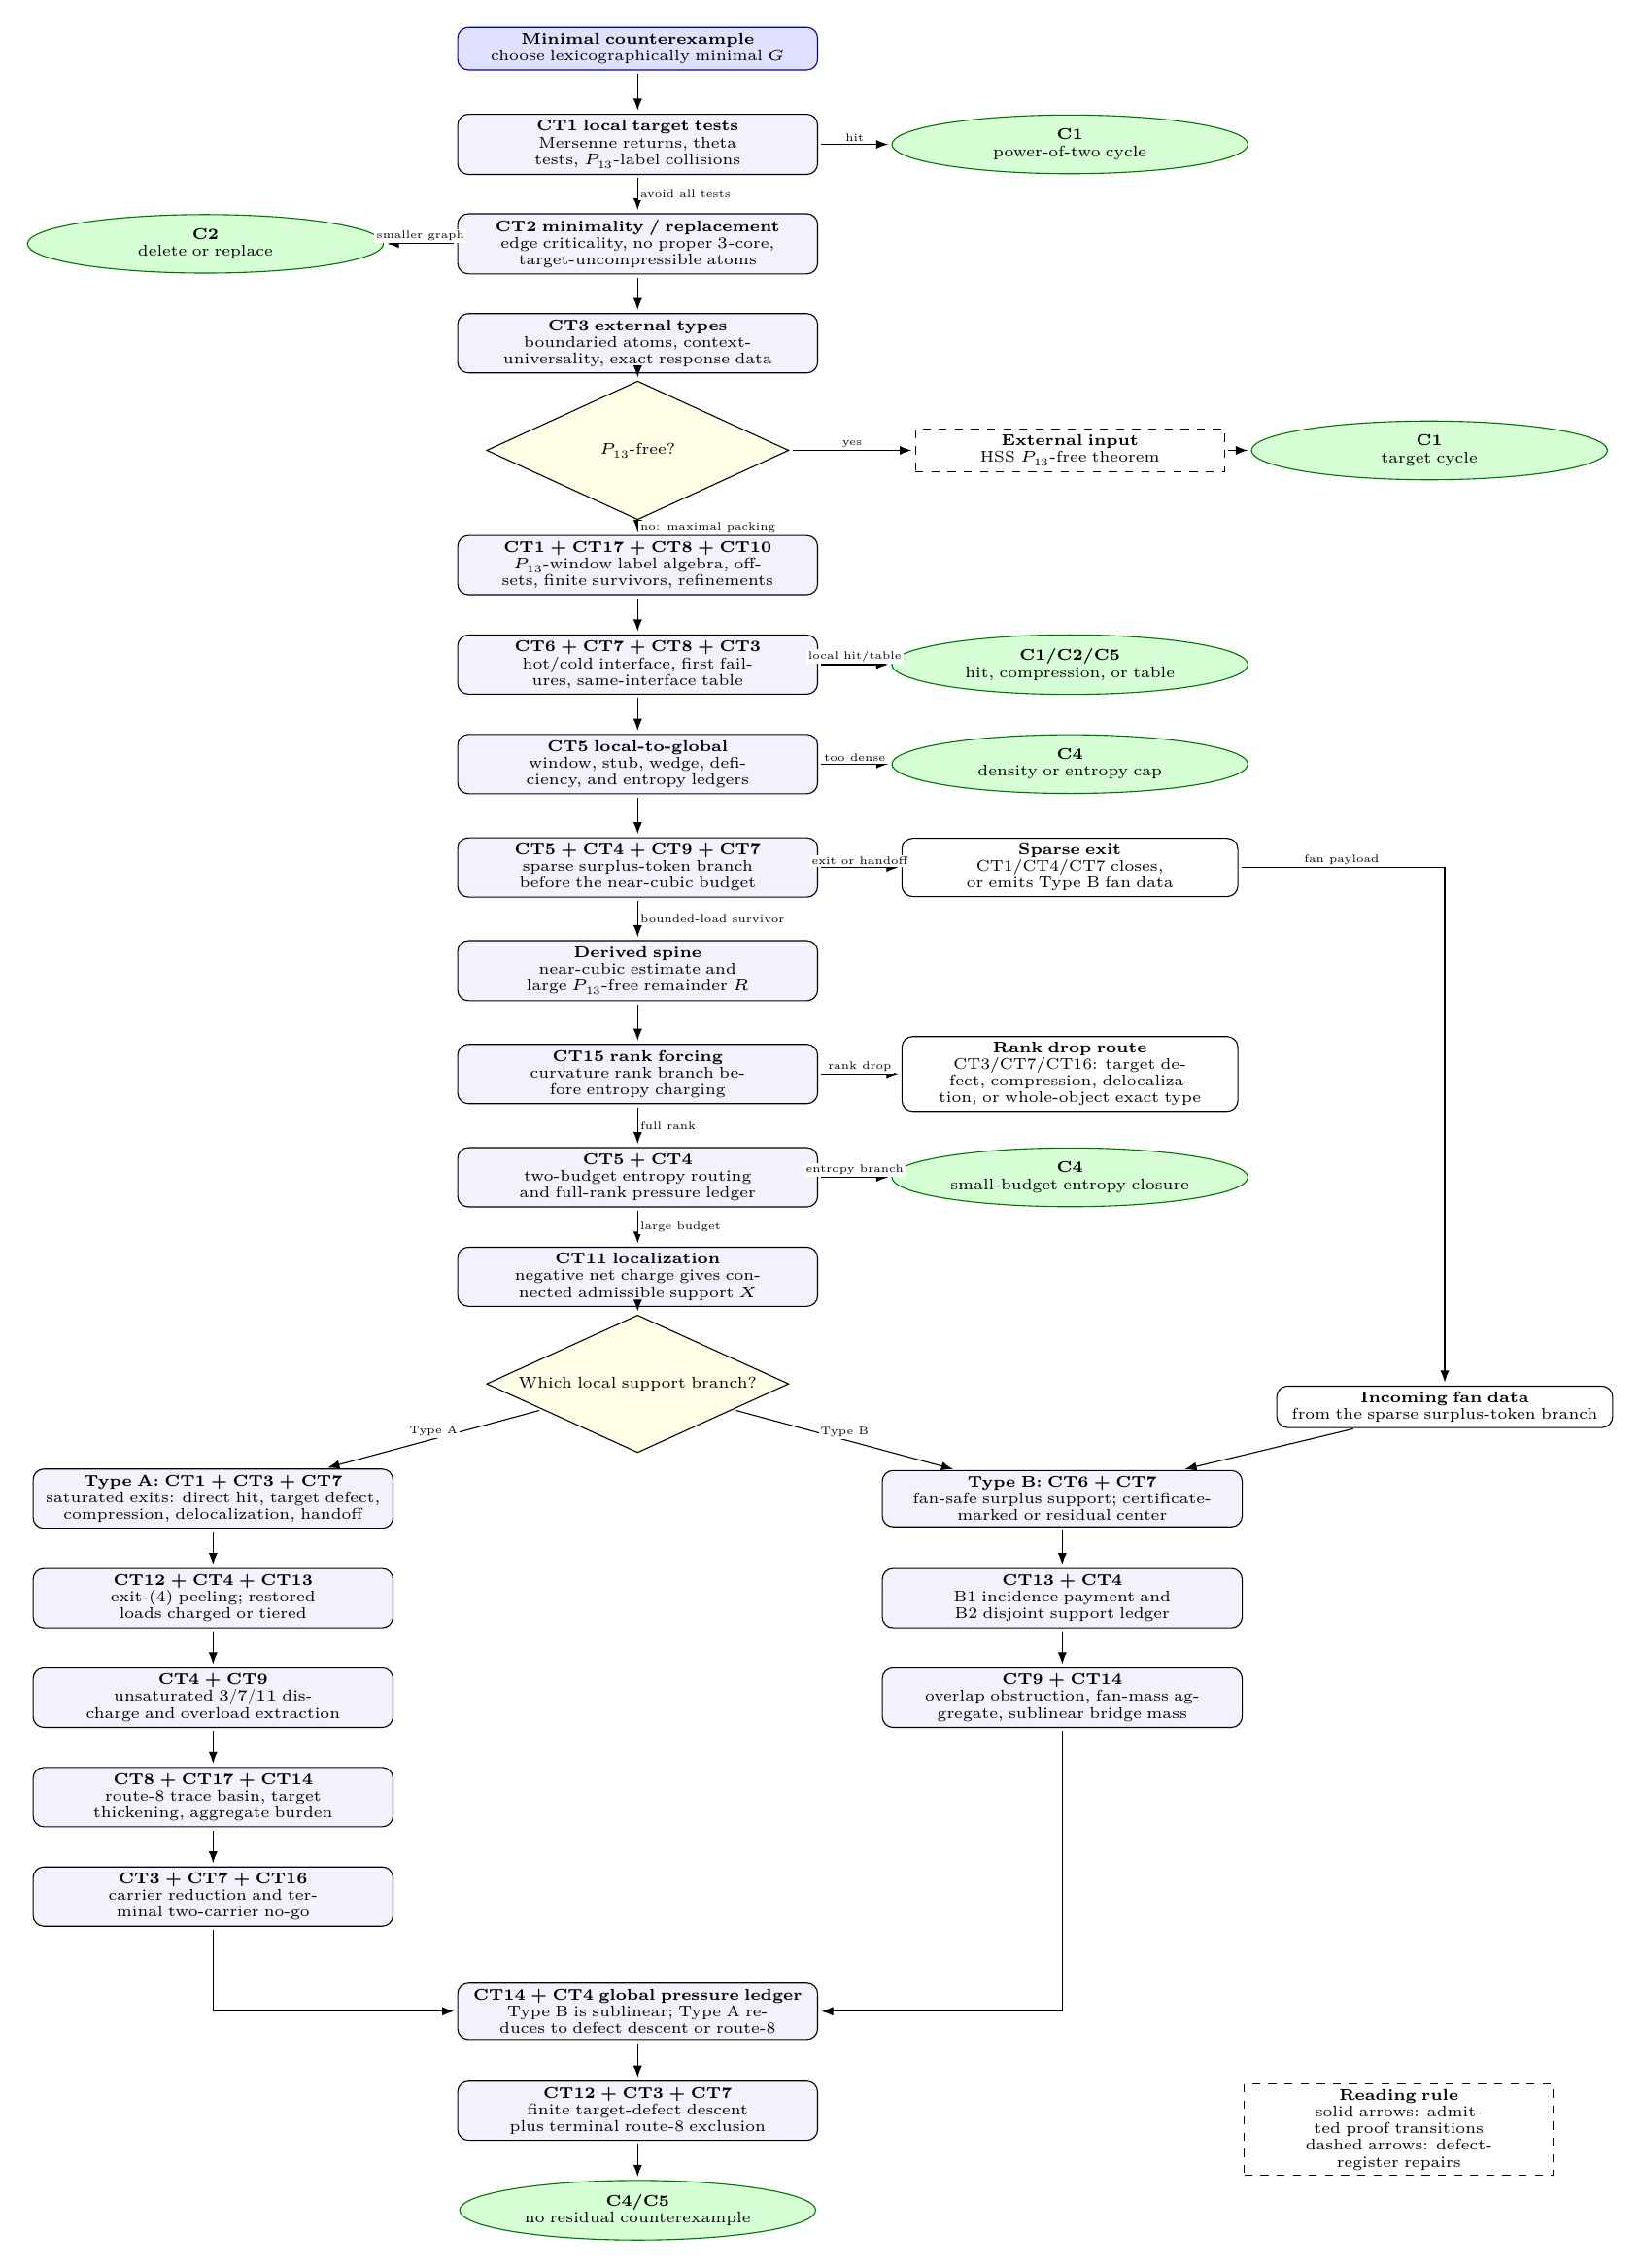
\begin{tikzpicture}[
x=1cm,
y=1cm,
every node/.style={font=\fontsize{5.8}{6.2}\selectfont},
stage/.style={rectangle,rounded corners,draw,fill=blue!5,align=center,inner sep=2.2pt,minimum width=4.55cm,text width=4.55cm},
setup/.style={stage,fill=blue!12,draw=blue!65!black},
test/.style={diamond,draw,fill=yellow!10,aspect=2.15,align=center,inner sep=1.0pt,minimum width=3.95cm,text width=3.25cm},
side/.style={rectangle,rounded corners,draw,fill=white,align=center,inner sep=2.0pt,minimum width=4.25cm,text width=4.25cm},
close/.style={ellipse,draw=green!45!black,fill=green!16,align=center,inner sep=2.0pt,minimum width=3.15cm,text width=3.15cm},
external/.style={rectangle,draw,dashed,align=center,inner sep=2.0pt,minimum width=3.90cm,text width=3.90cm},
arr/.style={-{Latex[length=1.55mm]},thin,shorten <=1.2pt,shorten >=1.2pt},
route/.style={-{Latex[length=1.55mm]},thin,shorten <=1.2pt,shorten >=1.2pt},
lbl/.style={font=\fontsize{4.0}{4.4}\selectfont,inner sep=0.8pt,fill=white}
]
\node[setup] (start) at (0,0) {\textbf{Minimal counterexample}\\choose lexicographically minimal \(G\)};
\node[stage] (target) at (0,-1.25) {\textbf{CT1 local target tests}\\Mersenne returns, theta tests, \(P_{13}\)-label collisions};
\node[close] (direct) at (5.65,-1.25) {\textbf{C1}\\power-of-two cycle};
\node[stage] (minimal) at (0,-2.55) {\textbf{CT2 minimality / replacement}\\edge criticality, no proper \(3\)-core, target-uncompressible atoms};
\node[close] (minclose) at (-5.65,-2.55) {\textbf{C2}\\delete or replace};
\node[stage] (types) at (0,-3.85) {\textbf{CT3 external types}\\boundaried atoms, context-universality, exact response data};
\node[test] (p13) at (0,-5.25) {\(P_{13}\)-free?};
\node[external] (hss) at (5.65,-5.25) {\textbf{External input}\\HSS \(P_{13}\)-free theorem};
\node[close] (hssclose) at (10.35,-5.25) {\textbf{C1}\\target cycle};

\node[stage] (windows) at (0,-6.75) {\textbf{CT1 + CT17 + CT8 + CT10}\\\(P_{13}\)-window label algebra, offsets, finite survivors, refinements};
\node[stage] (hotcold) at (0,-8.05) {\textbf{CT6 + CT7 + CT8 + CT3}\\hot/cold interface, first failures, same-interface table};
\node[close] (windowclose) at (5.65,-8.05) {\textbf{C1/C2/C5}\\hit, compression, or table};
\node[stage] (localglobal) at (0,-9.35) {\textbf{CT5 local-to-global}\\window, stub, wedge, deficiency, and entropy ledgers};
\node[close] (densityclose) at (5.65,-9.35) {\textbf{C4}\\density or entropy cap};
\node[stage] (surplus) at (0,-10.70) {\textbf{CT5 + CT4 + CT9 + CT7}\\sparse surplus-token branch before the near-cubic budget};
\node[side] (sparseexit) at (5.65,-10.70) {\textbf{Sparse exit}\\CT1/CT4/CT7 closes,\\or emits Type B fan data};
\node[stage] (spine) at (0,-12.05) {\textbf{Derived spine}\\near-cubic estimate and large \(P_{13}\)-free remainder \(R\)};
\node[stage] (rank) at (0,-13.40) {\textbf{CT15 rank forcing}\\curvature rank branch before entropy charging};
\node[side] (rankdrop) at (5.65,-13.40) {\textbf{Rank drop route}\\CT3/CT7/CT16: target defect, compression, delocalization, or whole-object exact type};
\node[stage] (budget) at (0,-14.75) {\textbf{CT5 + CT4}\\two-budget entropy routing and full-rank pressure ledger};
\node[close] (budgetclose) at (5.65,-14.75) {\textbf{C4}\\small-budget entropy closure};
\node[stage] (localize) at (0,-16.05) {\textbf{CT11 localization}\\negative net charge gives connected admissible support \(X\)};
\node[test] (split) at (0,-17.45) {Which local support branch?};

\node[stage] (typea1) at (-5.55,-18.95) {\textbf{Type A: CT1 + CT3 + CT7}\\saturated exits: direct hit, target defect, compression, delocalization, handoff};
\node[stage] (typea2) at (-5.55,-20.25) {\textbf{CT12 + CT4 + CT13}\\exit-(4) peeling; restored loads charged or tiered};
\node[stage] (typea3) at (-5.55,-21.55) {\textbf{CT4 + CT9}\\unsaturated \(3/7/11\) discharge and overload extraction};
\node[stage] (route8) at (-5.55,-22.85) {\textbf{CT8 + CT17 + CT14}\\route-8 trace basin, target thickening, aggregate burden};
\node[stage] (nogo) at (-5.55,-24.15) {\textbf{CT3 + CT7 + CT16}\\carrier reduction and terminal two-carrier no-go};

\node[stage] (typeb1) at (5.55,-18.95) {\textbf{Type B: CT6 + CT7}\\fan-safe surplus support; certificate-marked or residual center};
\node[stage] (typeb2) at (5.55,-20.25) {\textbf{CT13 + CT4}\\B1 incidence payment and B2 disjoint support ledger};
\node[stage] (typeb3) at (5.55,-21.55) {\textbf{CT9 + CT14}\\overlap obstruction, fan-mass aggregate, sublinear bridge mass};
\node[side] (typebfeed) at (10.55,-17.75) {\textbf{Incoming fan data}\\from the sparse surplus-token branch};

\node[stage] (join) at (0,-25.65) {\textbf{CT14 + CT4 global pressure ledger}\\Type B is sublinear; Type A reduces to defect descent or route-8};
\node[stage] (final) at (0,-26.95) {\textbf{CT12 + CT3 + CT7}\\finite target-defect descent plus terminal route-8 exclusion};
\node[close] (contradiction) at (0,-28.25) {\textbf{C4/C5}\\no residual counterexample};
\node[external] (legend) at (9.95,-27.20) {\textbf{Reading rule}\\solid arrows: admitted proof transitions\\dashed arrows: defect-register repairs};

\draw[arr] (start) -- (target);
\draw[arr] (target) -- node[lbl,above]{hit} (direct);
\draw[arr] (target) -- node[lbl,right]{avoid all tests} (minimal);
\draw[arr] (minimal) -- node[lbl,above]{smaller graph} (minclose);
\draw[arr] (minimal) -- (types);
\draw[arr] (types) -- (p13);
\draw[arr] (p13) -- node[lbl,above]{yes} (hss);
\draw[arr] (hss) -- (hssclose);
\draw[arr] (p13) -- node[lbl,right]{no: maximal packing} (windows);
\draw[arr] (windows) -- (hotcold);
\draw[arr] (hotcold) -- node[lbl,above]{local hit/table} (windowclose);
\draw[arr] (hotcold) -- (localglobal);
\draw[arr] (localglobal) -- node[lbl,above]{too dense} (densityclose);
\draw[arr] (localglobal) -- (surplus);
\draw[arr] (surplus) -- node[lbl,above]{exit or handoff} (sparseexit);
\draw[arr] (surplus) -- node[lbl,right]{bounded-load survivor} (spine);
\draw[arr] (spine) -- (rank);
\draw[arr] (rank) -- node[lbl,above]{rank drop} (rankdrop);
\draw[arr] (rank) -- node[lbl,right]{full rank} (budget);
\draw[arr] (budget) -- node[lbl,above]{entropy branch} (budgetclose);
\draw[arr] (budget) -- node[lbl,right]{large budget} (localize);
\draw[arr] (localize) -- (split);
\draw[arr] (split) -- node[lbl,above]{Type A} (typea1);
\draw[arr] (split) -- node[lbl,above]{Type B} (typeb1);
\draw[arr] (typea1) -- (typea2);
\draw[arr] (typea2) -- (typea3);
\draw[arr] (typea3) -- (route8);
\draw[arr] (route8) -- (nogo);
\draw[arr] (typeb1) -- (typeb2);
\draw[arr] (typeb2) -- (typeb3);
\coordinate (fanpayloadbend) at (10.55,-10.70);
\draw[route] (sparseexit.east) -- node[lbl,above]{fan payload} (fanpayloadbend) -- (typebfeed.north);
\draw[route] (typebfeed) -- (typeb1);
\draw[arr] (nogo) |- (join);
\draw[arr] (typeb3) |- (join);
\draw[arr] (join) -- (final);
\draw[arr] (final) -- (contradiction);
\end{tikzpicture}%
}
\caption[EG aggregate CT proof-flow chart]{EG aggregate CT proof-flow chart.  This one-page version groups consecutive tactic applications into proof segments while preserving the top-to-bottom architecture of {[}EG{]}.  The six detailed panels in Figs.~\ref{fig:eg-high-level-ct-flow-i}--\ref{fig:eg-high-level-ct-flow-vi} expand the same load path CT by CT\@.}
\label{fig:eg-high-level-ct-flow}
\label{fig:eg-aggregate-ct-flow}
\end{figure}

\begin{figure}[p]
\centering
\vspace*{-6.75cm}
\resizebox{0.92\textwidth}{!}{%
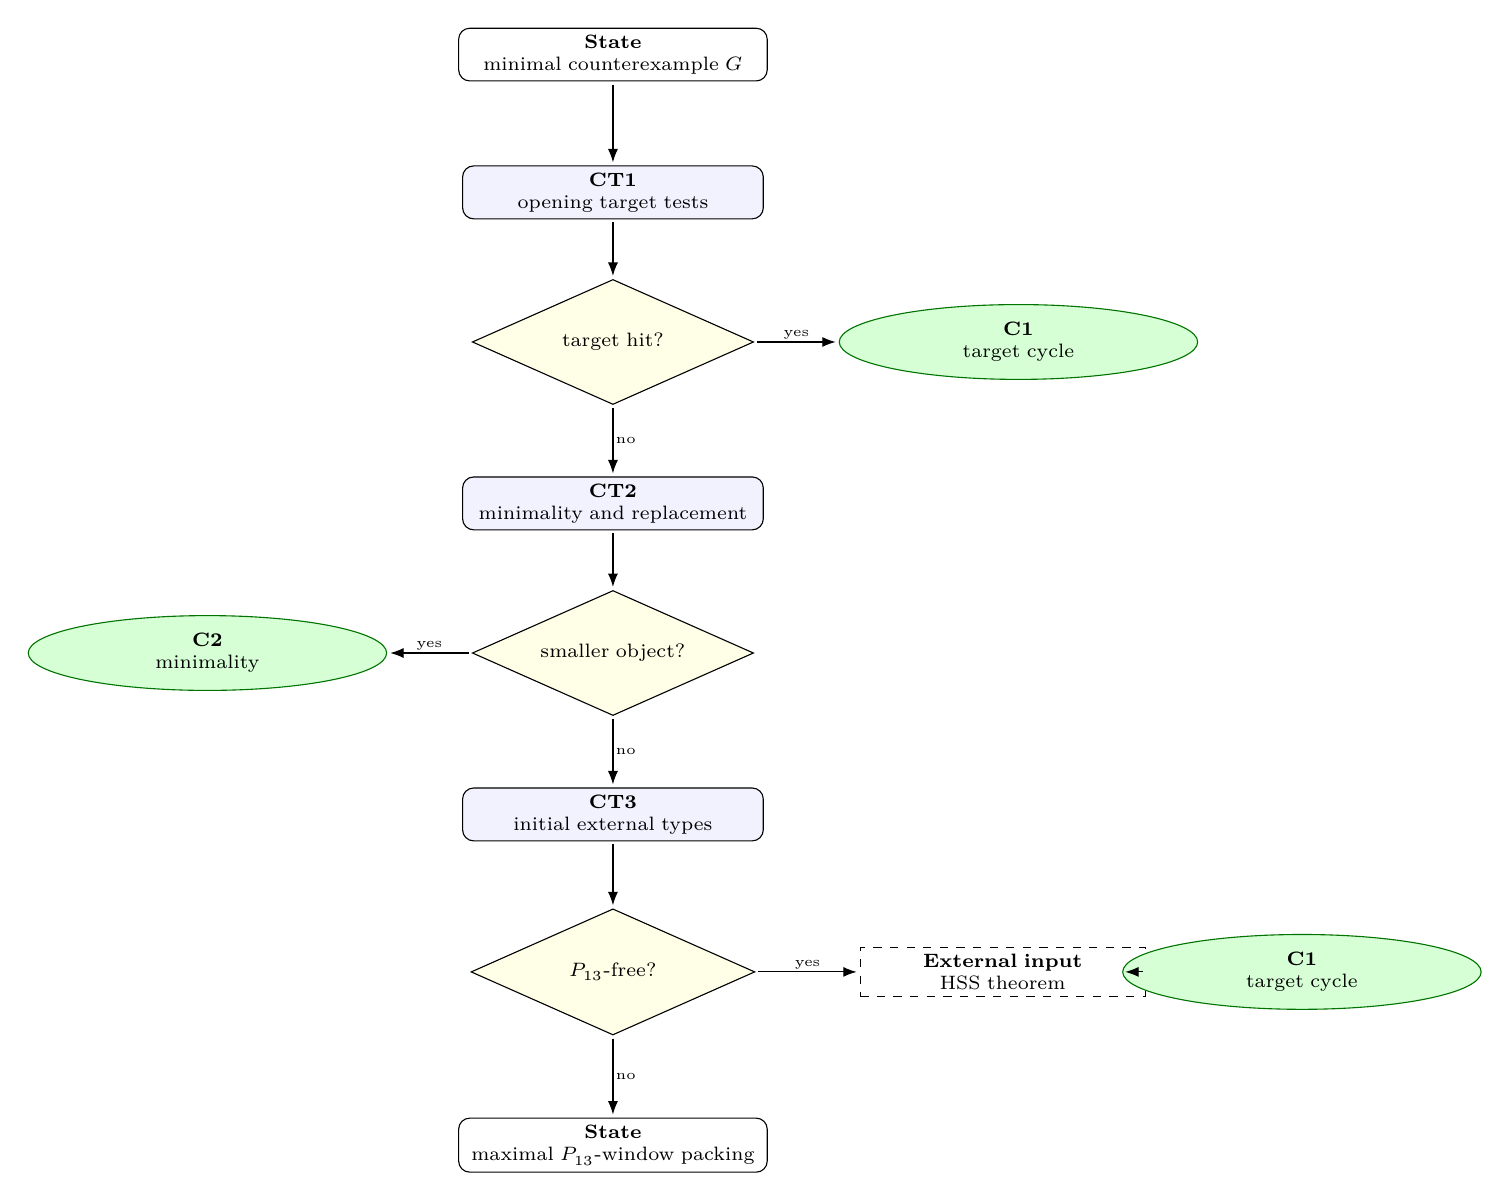
\begin{tikzpicture}[
x=1cm,
y=1cm,
every node/.style={font=\scriptsize},
tactic/.style={rectangle,rounded corners,draw,fill=blue!5,align=center,inner sep=2.4pt,minimum width=3.65cm,text width=3.65cm},
state/.style={rectangle,rounded corners,draw,fill=white,align=center,inner sep=2.4pt,minimum width=3.75cm,text width=3.75cm},
test/.style={diamond,draw,fill=yellow!10,aspect=2.25,align=center,inner sep=1.4pt,minimum width=3.45cm,text width=2.75cm},
close/.style={ellipse,draw=green!45!black,fill=green!16,align=center,inner sep=2.4pt,minimum width=3.05cm,text width=3.05cm},
external/.style={rectangle,draw,dashed,align=center,inner sep=2.4pt,minimum width=3.45cm,text width=3.45cm},
arr/.style={-{Latex[length=1.7mm]},thin,shorten <=1.1pt,shorten >=1.1pt},
lbl/.style={font=\tiny,inner sep=0.9pt,fill=white}
]
\node[state] (start) at (0,2.00) {\textbf{State}\\minimal counterexample \(G\)};
\node[tactic] (ct1) at (0,0.25) {\textbf{CT1}\\opening target tests};
\node[test] (target) at (0,-1.65) {target hit?};
\node[close] (c1) at (5.15,-1.65) {\textbf{C1}\\target cycle};
\node[tactic] (ct2) at (0,-3.70) {\textbf{CT2}\\minimality and replacement};
\node[test] (small) at (0,-5.60) {smaller object?};
\node[close] (c2) at (-5.15,-5.60) {\textbf{C2}\\minimality};
\node[tactic] (ct3) at (0,-7.65) {\textbf{CT3}\\initial external types};
\node[test] (p13) at (0,-9.65) {\(P_{13}\)-free?};
\node[external] (hss) at (4.95,-9.65) {\textbf{External input}\\HSS theorem};
\node[close] (hssc) at (8.75,-9.65) {\textbf{C1}\\target cycle};
\node[state] (pack) at (0,-11.85) {\textbf{State}\\maximal \(P_{13}\)-window packing};

\draw[arr] (start) -- (ct1);
\draw[arr] (ct1) -- (target);
\draw[arr] (target) -- node[lbl,above]{yes} (c1);
\draw[arr] (target) -- node[lbl,right]{no} (ct2);
\draw[arr] (ct2) -- (small);
\draw[arr] (small) -- node[lbl,above]{yes} (c2);
\draw[arr] (small) -- node[lbl,right]{no} (ct3);
\draw[arr] (ct3) -- (p13);
\draw[arr] (p13) -- node[lbl,above]{yes} (hss);
\draw[arr] (hss) -- (hssc);
\draw[arr] (p13) -- node[lbl,right]{no} (pack);
\end{tikzpicture}%
}
\caption[EG high-level CT proof-flow chart I]{EG high-level CT proof-flow chart I.  The first detailed panel starts with the minimal counterexample and ends at the maximal \(P_{13}\)-window packing, which is repeated as the first node of Fig.~\ref{fig:eg-high-level-ct-flow-ii}.}
\label{fig:eg-high-level-ct-flow-i}
\vspace*{6.75cm}
\end{figure}

\begin{figure}[p]
\centering
\vspace*{-4.85cm}
\resizebox{!}{1.04\textheight}{%
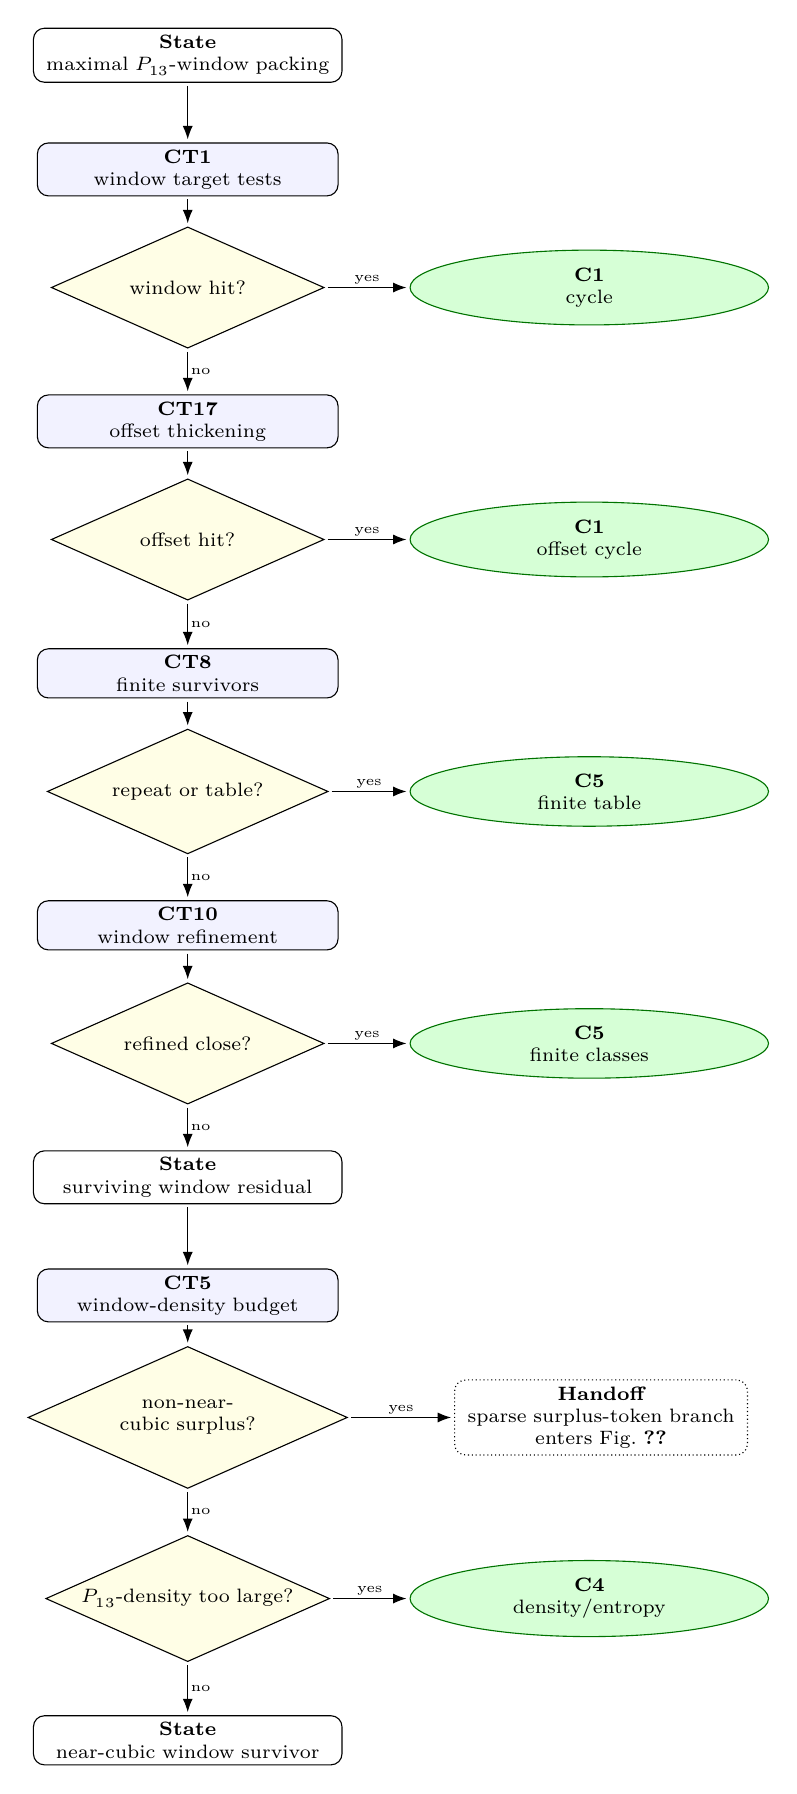
\begin{tikzpicture}[
x=1cm,
y=1cm,
every node/.style={font=\scriptsize},
tactic/.style={rectangle,rounded corners,draw,fill=blue!5,align=center,inner sep=2.4pt,minimum width=3.65cm,text width=3.65cm},
state/.style={rectangle,rounded corners,draw,fill=white,align=center,inner sep=2.4pt,minimum width=3.75cm,text width=3.75cm},
test/.style={diamond,draw,fill=yellow!10,aspect=2.25,align=center,inner sep=1.4pt,minimum width=3.45cm,text width=2.75cm},
close/.style={ellipse,draw=green!45!black,fill=green!16,align=center,inner sep=2.4pt,minimum width=3.05cm,text width=3.05cm},
handoff/.style={rectangle,rounded corners,draw,densely dotted,align=center,inner sep=2.4pt,minimum width=3.55cm,text width=3.55cm},
arr/.style={-{Latex[length=1.7mm]},thin,shorten <=1.1pt,shorten >=1.1pt},
lbl/.style={font=\tiny,inner sep=0.9pt,fill=white}
]
\node[state] (pack) at (0,0) {\textbf{State}\\maximal \(P_{13}\)-window packing};
\node[tactic] (ct1w) at (0,-1.45) {\textbf{CT1}\\window target tests};
\node[test] (hit) at (0,-2.95) {window hit?};
\node[close] (c1hit) at (5.10,-2.95) {\textbf{C1}\\cycle};
\node[tactic] (ct17) at (0,-4.65) {\textbf{CT17}\\offset thickening};
\node[test] (offset) at (0,-6.15) {offset hit?};
\node[close] (c1off) at (5.10,-6.15) {\textbf{C1}\\offset cycle};
\node[tactic] (ct8) at (0,-7.85) {\textbf{CT8}\\finite survivors};
\node[test] (table) at (0,-9.35) {repeat or table?};
\node[close] (c5table) at (5.10,-9.35) {\textbf{C5}\\finite table};
\node[tactic] (ct10) at (0,-11.05) {\textbf{CT10}\\window refinement};
\node[test] (refined) at (0,-12.55) {refined close?};
\node[close] (c5ref) at (5.10,-12.55) {\textbf{C5}\\finite classes};
\node[state] (residual) at (0,-14.25) {\textbf{State}\\surviving window residual};
\node[tactic] (ct5density) at (0,-15.75) {\textbf{CT5}\\window-density budget};
\node[test] (surplus) at (0,-17.30) {non-near-cubic surplus?};
\node[handoff] (surphandoff) at (5.25,-17.30) {\textbf{Handoff}\\sparse surplus-token branch\\enters Fig.~\ref{fig:eg-high-level-ct-flow-iv}};
\node[test] (dense) at (0,-19.60) {\(P_{13}\)-density too large?};
\node[close] (c4dense) at (5.10,-19.60) {\textbf{C4}\\density/entropy};
\node[state] (nearwin) at (0,-21.40) {\textbf{State}\\near-cubic window survivor};

\draw[arr] (pack) -- (ct1w);
\draw[arr] (ct1w) -- (hit);
\draw[arr] (hit) -- node[lbl,above]{yes} (c1hit);
\draw[arr] (hit) -- node[lbl,right]{no} (ct17);
\draw[arr] (ct17) -- (offset);
\draw[arr] (offset) -- node[lbl,above]{yes} (c1off);
\draw[arr] (offset) -- node[lbl,right]{no} (ct8);
\draw[arr] (ct8) -- (table);
\draw[arr] (table) -- node[lbl,above]{yes} (c5table);
\draw[arr] (table) -- node[lbl,right]{no} (ct10);
\draw[arr] (ct10) -- (refined);
\draw[arr] (refined) -- node[lbl,above]{yes} (c5ref);
\draw[arr] (refined) -- node[lbl,right]{no} (residual);
\draw[arr] (residual) -- (ct5density);
\draw[arr] (ct5density) -- (surplus);
\draw[arr] (surplus) -- node[lbl,above]{yes} (surphandoff);
\draw[arr] (surplus) -- node[lbl,right]{no} (dense);
\draw[arr] (dense) -- node[lbl,above]{yes} (c4dense);
\draw[arr] (dense) -- node[lbl,right]{no} (nearwin);
\end{tikzpicture}%
}
\caption[EG high-level CT proof-flow chart II]{EG high-level CT proof-flow chart II\@.  The second detailed panel starts with the maximal \(P_{13}\)-window packing, performs the window target, offset, finite-survivor, refinement, and density-budget tests, and ends at the near-cubic window survivor.  The non-near-cubic surplus branch is not terminal; its typed handoff enters Fig.~\ref{fig:eg-high-level-ct-flow-iv}.}
\label{fig:eg-high-level-ct-flow-ii}
\vspace*{0.25cm}
\end{figure}

\begin{figure}[p]
\centering
\vspace*{-4.10cm}
\resizebox{!}{0.74\textheight}{%
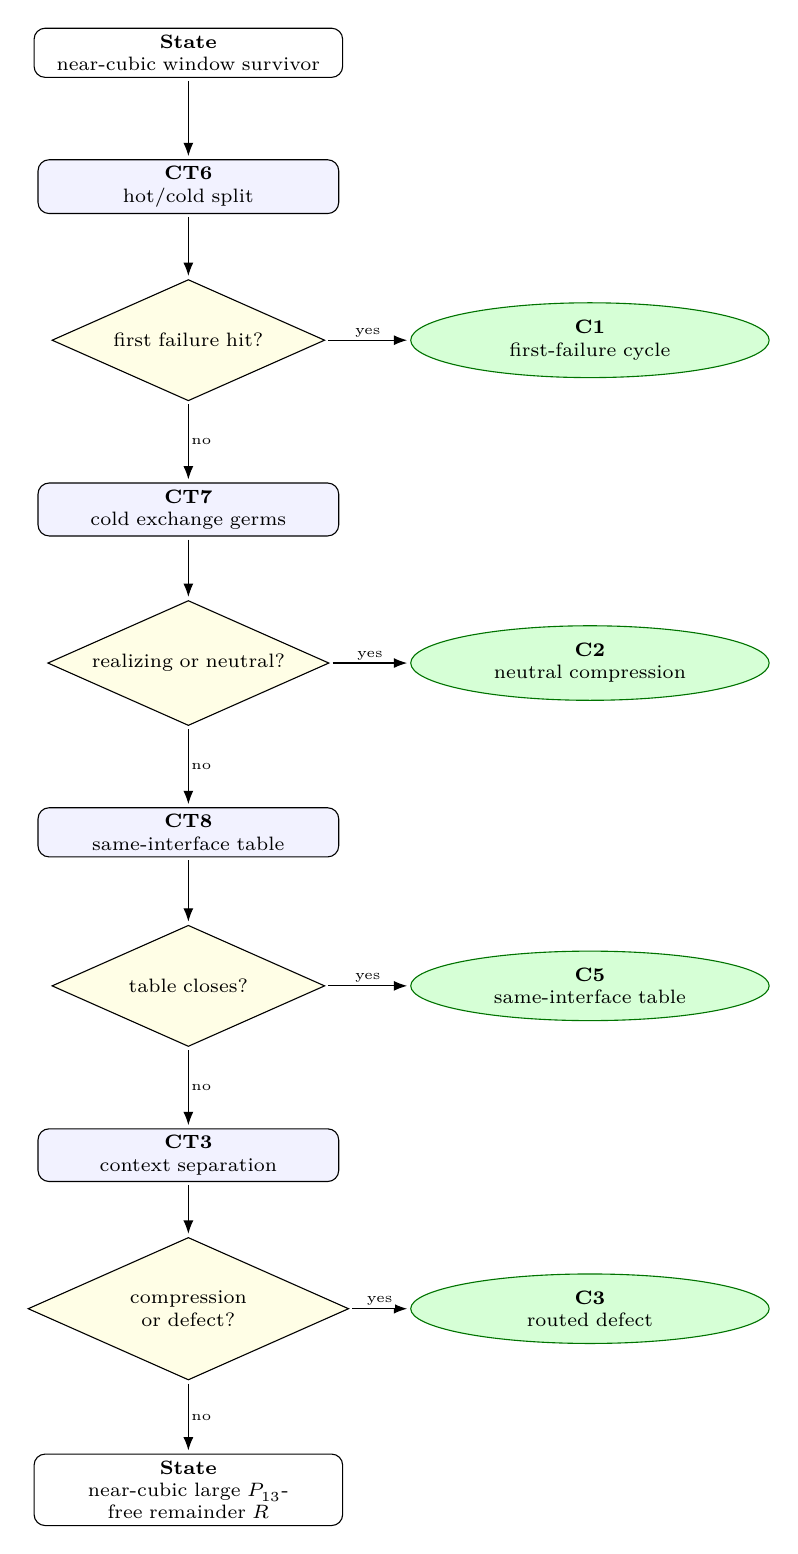
\begin{tikzpicture}[
x=1cm,
y=1cm,
every node/.style={font=\scriptsize},
tactic/.style={rectangle,rounded corners,draw,fill=blue!5,align=center,inner sep=2.4pt,minimum width=3.65cm,text width=3.65cm},
state/.style={rectangle,rounded corners,draw,fill=white,align=center,inner sep=2.4pt,minimum width=3.75cm,text width=3.75cm},
test/.style={diamond,draw,fill=yellow!10,aspect=2.25,align=center,inner sep=1.4pt,minimum width=3.45cm,text width=2.75cm},
close/.style={ellipse,draw=green!45!black,fill=green!16,align=center,inner sep=2.4pt,minimum width=3.05cm,text width=3.05cm},
arr/.style={-{Latex[length=1.7mm]},thin,shorten <=1.1pt,shorten >=1.1pt},
lbl/.style={font=\tiny,inner sep=0.9pt,fill=white}
]
\node[state] (nearwin) at (0,1.70) {\textbf{State}\\near-cubic window survivor};
\node[tactic] (ct6) at (0,0.00) {\textbf{CT6}\\hot/cold split};
\node[test] (first) at (0,-1.95) {first failure hit?};
\node[close] (c1) at (5.10,-1.95) {\textbf{C1}\\first-failure cycle};
\node[tactic] (ct7) at (0,-4.10) {\textbf{CT7}\\cold exchange germs};
\node[test] (neutral) at (0,-6.05) {realizing or neutral?};
\node[close] (c2) at (5.10,-6.05) {\textbf{C2}\\neutral compression};
\node[tactic] (ct8) at (0,-8.20) {\textbf{CT8}\\same-interface table};
\node[test] (table) at (0,-10.15) {table closes?};
\node[close] (c5) at (5.10,-10.15) {\textbf{C5}\\same-interface table};
\node[tactic] (ct3) at (0,-12.30) {\textbf{CT3}\\context separation};
\node[test] (defect) at (0,-14.25) {compression or defect?};
\node[close] (c3) at (5.10,-14.25) {\textbf{C3}\\routed defect};
\node[state] (remainder) at (0,-16.55) {\textbf{State}\\near-cubic large \(P_{13}\)-free remainder \(R\)};

\draw[arr] (nearwin) -- (ct6);
\draw[arr] (ct6) -- (first);
\draw[arr] (first) -- node[lbl,above]{yes} (c1);
\draw[arr] (first) -- node[lbl,right]{no} (ct7);
\draw[arr] (ct7) -- (neutral);
\draw[arr] (neutral) -- node[lbl,above]{yes} (c2);
\draw[arr] (neutral) -- node[lbl,right]{no} (ct8);
\draw[arr] (ct8) -- (table);
\draw[arr] (table) -- node[lbl,above]{yes} (c5);
\draw[arr] (table) -- node[lbl,right]{no} (ct3);
\draw[arr] (ct3) -- (defect);
\draw[arr] (defect) -- node[lbl,above]{yes} (c3);
\draw[arr] (defect) -- node[lbl,right]{no} (remainder);
\end{tikzpicture}%
}
\caption[EG high-level CT proof-flow chart III]{EG high-level CT proof-flow chart III\@.  The third detailed panel expands the hot/cold window interface.  Its surviving branch is the near-cubic large \(P_{13}\)-free remainder \(R\), repeated as the first node of Fig.~\ref{fig:eg-high-level-ct-flow-iv}.}
\label{fig:eg-high-level-ct-flow-iii}
\vspace*{4.10cm}
\end{figure}

\begin{figure}[p]
\centering
\vspace*{-3.75cm}
\resizebox{!}{0.88\textheight}{%
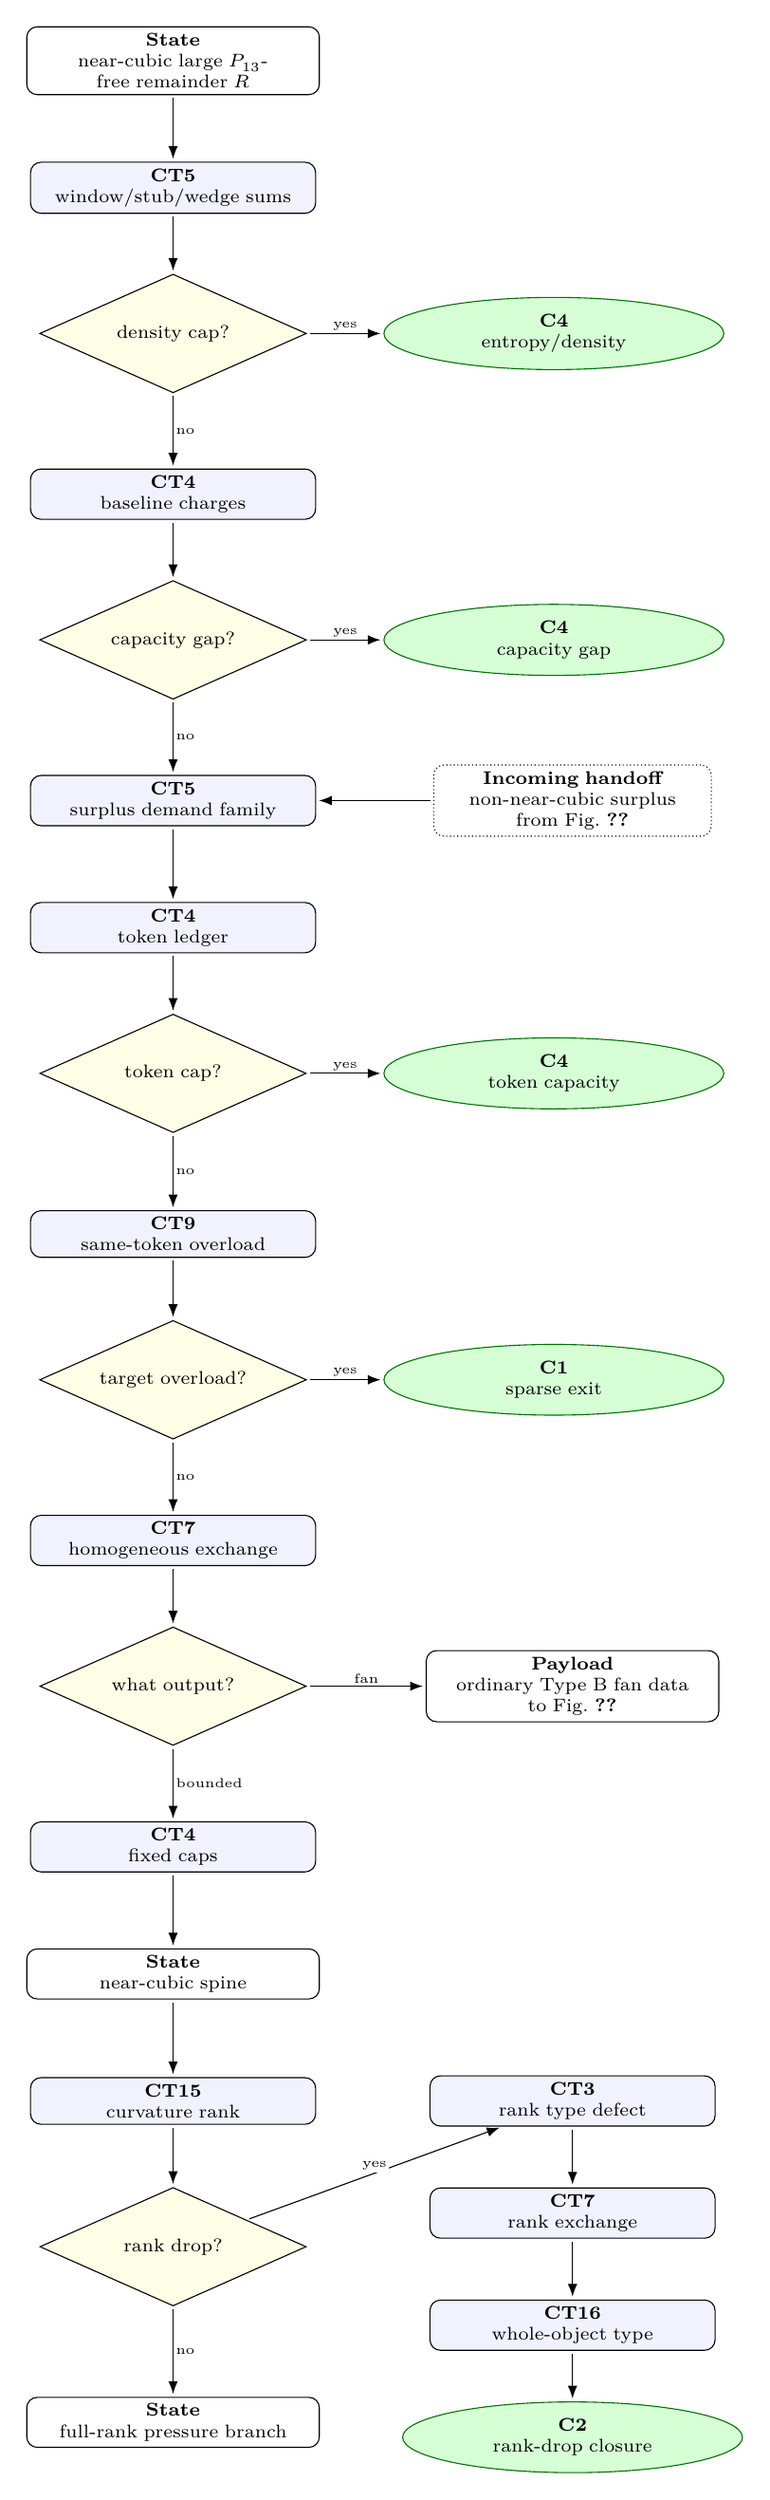
\begin{tikzpicture}[
x=1cm,
y=1cm,
every node/.style={font=\scriptsize},
tactic/.style={rectangle,rounded corners,draw,fill=blue!5,align=center,inner sep=2.4pt,minimum width=3.65cm,text width=3.65cm},
state/.style={rectangle,rounded corners,draw,fill=white,align=center,inner sep=2.4pt,minimum width=3.75cm,text width=3.75cm},
test/.style={diamond,draw,fill=yellow!10,aspect=2.25,align=center,inner sep=1.4pt,minimum width=3.45cm,text width=2.75cm},
close/.style={ellipse,draw=green!45!black,fill=green!16,align=center,inner sep=2.4pt,minimum width=3.05cm,text width=3.05cm},
handoff/.style={rectangle,rounded corners,draw,densely dotted,align=center,inner sep=2.4pt,minimum width=3.55cm,text width=3.55cm},
arr/.style={-{Latex[length=1.7mm]},thin,shorten <=1.1pt,shorten >=1.1pt},
route/.style={-{Latex[length=1.7mm]},thin,shorten <=1.1pt,shorten >=1.1pt},
lbl/.style={font=\tiny,inner sep=0.9pt,fill=white}
]
\node[state] (rem) at (0,1.60) {\textbf{State}\\near-cubic large \(P_{13}\)-free remainder \(R\)};
\node[tactic] (ct5) at (0,-0.10) {\textbf{CT5}\\window/stub/wedge sums};
\node[test] (density) at (0,-2.05) {density cap?};
\node[close] (c4density) at (5.10,-2.05) {\textbf{C4}\\entropy/density};
\node[tactic] (ct4base) at (0,-4.20) {\textbf{CT4}\\baseline charges};
\node[test] (capacity) at (0,-6.15) {capacity gap?};
\node[close] (c4base) at (5.10,-6.15) {\textbf{C4}\\capacity gap};
\node[tactic] (ct5surp) at (0,-8.30) {\textbf{CT5}\\surplus demand family};
\node[handoff] (surpin) at (5.35,-8.30) {\textbf{Incoming handoff}\\non-near-cubic surplus\\from Fig.~\ref{fig:eg-high-level-ct-flow-ii}};
\node[tactic] (ct4tok) at (0,-10.00) {\textbf{CT4}\\token ledger};
\node[test] (tokcap) at (0,-11.95) {token cap?};
\node[close] (c4tok) at (5.10,-11.95) {\textbf{C4}\\token capacity};
\node[tactic] (ct9) at (0,-14.10) {\textbf{CT9}\\same-token overload};
\node[test] (over) at (0,-16.05) {target overload?};
\node[close] (c1sparse) at (5.10,-16.05) {\textbf{C1}\\sparse exit};
\node[tactic] (ct7) at (0,-18.20) {\textbf{CT7}\\homogeneous exchange};
\node[test] (out) at (0,-20.15) {what output?};
\node[state] (fan) at (5.35,-20.15) {\textbf{Payload}\\ordinary Type B fan data\\to Fig.~\ref{fig:eg-high-level-ct-flow-vi}};
\node[tactic] (ct4caps) at (0,-22.30) {\textbf{CT4}\\fixed caps};
\node[state] (spine) at (0,-24.00) {\textbf{State}\\near-cubic spine};
\node[tactic] (ct15) at (0,-25.70) {\textbf{CT15}\\curvature rank};
\node[test] (rank) at (0,-27.65) {rank drop?};
\node[tactic] (ct3r) at (5.35,-25.70) {\textbf{CT3}\\rank type defect};
\node[tactic] (ct7r) at (5.35,-27.20) {\textbf{CT7}\\rank exchange};
\node[tactic] (ct16r) at (5.35,-28.70) {\textbf{CT16}\\whole-object type};
\node[close] (c2rank) at (5.35,-30.20) {\textbf{C2}\\rank-drop closure};
\node[state] (fullrank) at (0,-30.00) {\textbf{State}\\full-rank pressure branch};

\draw[arr] (rem) -- (ct5);
\draw[arr] (ct5) -- (density);
\draw[arr] (density) -- node[lbl,above]{yes} (c4density);
\draw[arr] (density) -- node[lbl,right]{no} (ct4base);
\draw[arr] (ct4base) -- (capacity);
\draw[arr] (capacity) -- node[lbl,above]{yes} (c4base);
\draw[arr] (capacity) -- node[lbl,right]{no} (ct5surp);
\draw[route] (surpin) -- (ct5surp);
\draw[arr] (ct5surp) -- (ct4tok);
\draw[arr] (ct4tok) -- (tokcap);
\draw[arr] (tokcap) -- node[lbl,above]{yes} (c4tok);
\draw[arr] (tokcap) -- node[lbl,right]{no} (ct9);
\draw[arr] (ct9) -- (over);
\draw[arr] (over) -- node[lbl,above]{yes} (c1sparse);
\draw[arr] (over) -- node[lbl,right]{no} (ct7);
\draw[arr] (ct7) -- (out);
\draw[arr] (out) -- node[lbl,above]{fan} (fan);
\draw[arr] (out) -- node[lbl,right]{bounded} (ct4caps);
\draw[arr] (ct4caps) -- (spine);
\draw[arr] (spine) -- (ct15);
\draw[arr] (ct15) -- (rank);
\draw[arr] (rank) -- node[lbl,above]{yes} (ct3r);
\draw[arr] (ct3r) -- (ct7r);
\draw[arr] (ct7r) -- (ct16r);
\draw[arr] (ct16r) -- (c2rank);
\draw[arr] (rank) -- node[lbl,right]{no} (fullrank);
\end{tikzpicture}%
}
\caption[EG high-level CT proof-flow chart IV]{EG high-level CT proof-flow chart IV\@.  The fourth detailed panel starts from the near-cubic large \(P_{13}\)-free remainder, incorporates the non-near-cubic surplus handoff from Fig.~\ref{fig:eg-high-level-ct-flow-ii}, runs the surplus-token branch, and ends at the full-rank pressure branch.  Ordinary Type B fan data is emitted as a typed payload for Fig.~\ref{fig:eg-high-level-ct-flow-vi}.}
\label{fig:eg-high-level-ct-flow-iv}
\end{figure}

\begin{figure}[p]
\centering
\vspace*{-2.00cm}
\resizebox{!}{0.80\textheight}{%
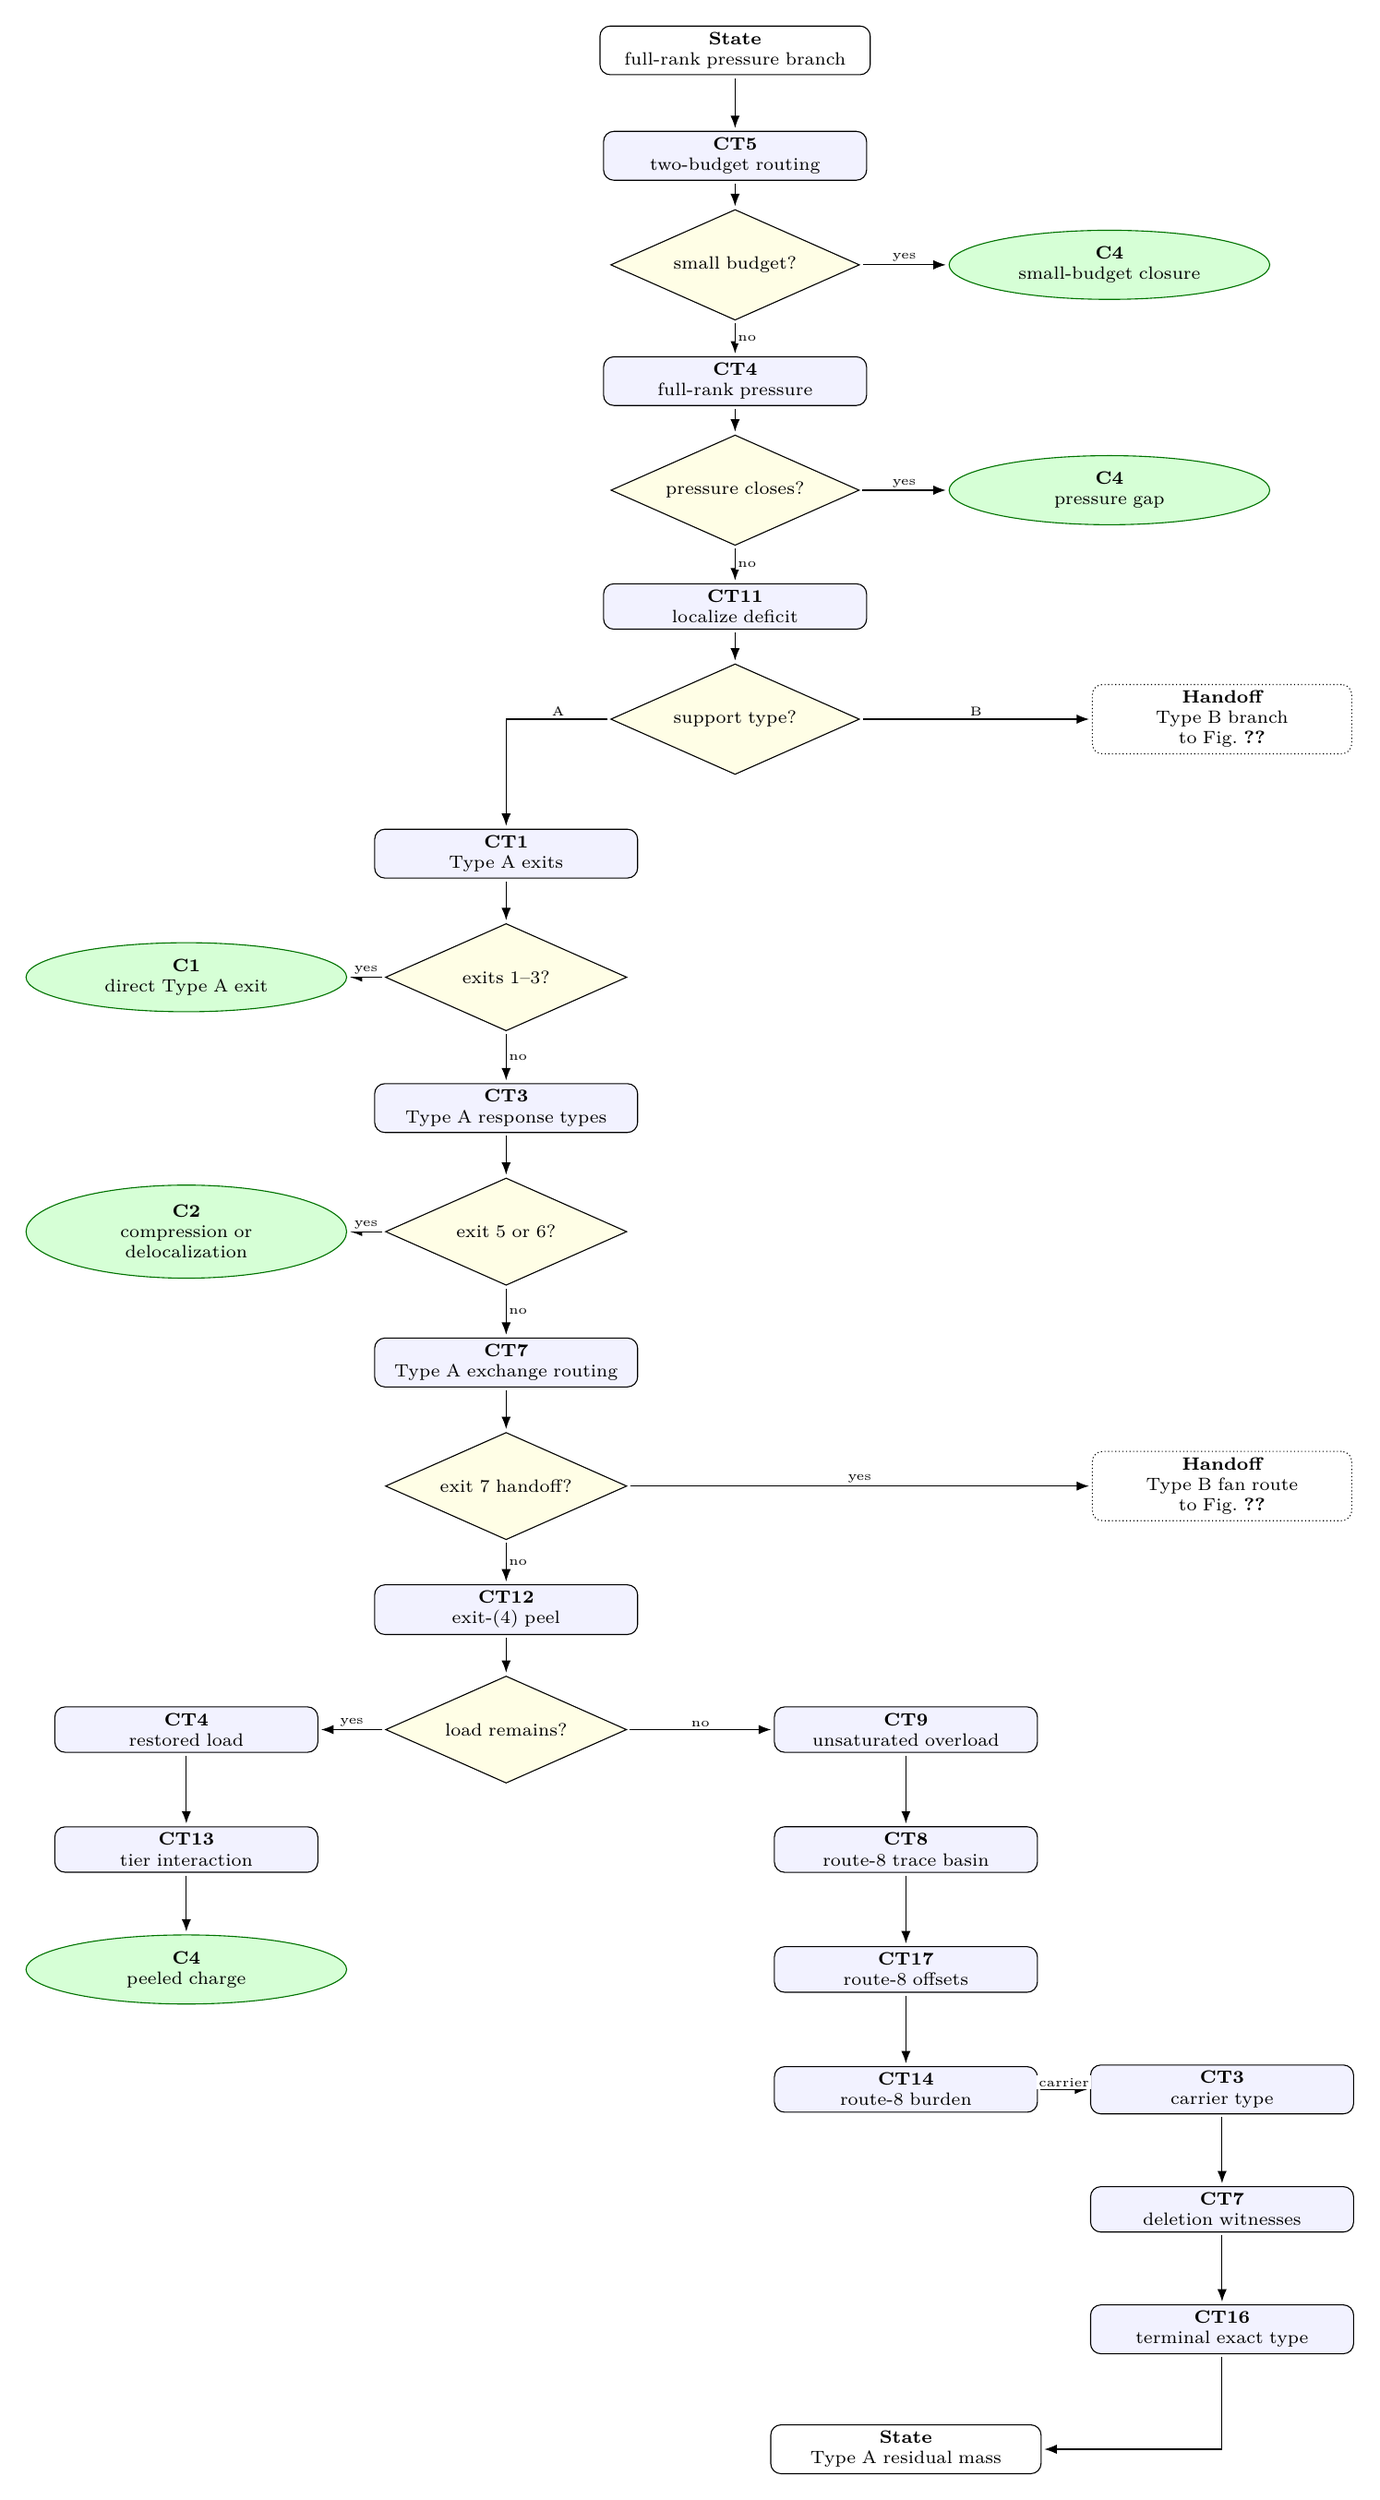
\begin{tikzpicture}[
x=1cm,
y=1cm,
every node/.style={font=\scriptsize},
tactic/.style={rectangle,rounded corners,draw,fill=blue!5,align=center,inner sep=2.4pt,minimum width=3.45cm,text width=3.45cm},
state/.style={rectangle,rounded corners,draw,fill=white,align=center,inner sep=2.4pt,minimum width=3.55cm,text width=3.55cm},
test/.style={diamond,draw,fill=yellow!10,aspect=2.25,align=center,inner sep=1.4pt,minimum width=3.25cm,text width=2.60cm},
close/.style={ellipse,draw=green!45!black,fill=green!16,align=center,inner sep=2.4pt,minimum width=2.95cm,text width=2.95cm},
handoff/.style={rectangle,rounded corners,draw,densely dotted,align=center,inner sep=2.4pt,minimum width=3.40cm,text width=3.40cm},
arr/.style={-{Latex[length=1.7mm]},thin,shorten <=1.1pt,shorten >=1.1pt},
route/.style={-{Latex[length=1.7mm]},thin,shorten <=1.1pt,shorten >=1.1pt},
lbl/.style={font=\tiny,inner sep=0.9pt,fill=white}
]
\node[state] (fullrank) at (0,0) {\textbf{State}\\full-rank pressure branch};
\node[tactic] (ct5two) at (0,-1.45) {\textbf{CT5}\\two-budget routing};
\node[test] (small) at (0,-2.95) {small budget?};
\node[close] (c4small) at (5.15,-2.95) {\textbf{C4}\\small-budget closure};
\node[tactic] (ct4press) at (0,-4.55) {\textbf{CT4}\\full-rank pressure};
\node[test] (press) at (0,-6.05) {pressure closes?};
\node[close] (c4press) at (5.15,-6.05) {\textbf{C4}\\pressure gap};
\node[tactic] (ct11) at (0,-7.65) {\textbf{CT11}\\localize deficit};
\node[test] (support) at (0,-9.20) {support type?};
\node[handoff] (bhand) at (6.70,-9.20) {\textbf{Handoff}\\Type B branch\\to Fig.~\ref{fig:eg-high-level-ct-flow-vi}};

\node[tactic] (ct1a) at (-3.15,-11.05) {\textbf{CT1}\\Type A exits};
\node[test] (aexits) at (-3.15,-12.75) {exits 1--3?};
\node[close] (c1a) at (-7.55,-12.75) {\textbf{C1}\\direct Type A exit};
\node[tactic] (ct3a) at (-3.15,-14.55) {\textbf{CT3}\\Type A response types};
\node[test] (acomp) at (-3.15,-16.25) {exit 5 or 6?};
\node[close] (c2a) at (-7.55,-16.25) {\textbf{C2}\\compression or delocalization};
\node[tactic] (ct7a) at (-3.15,-18.05) {\textbf{CT7}\\Type A exchange routing};
\node[test] (handoffq) at (-3.15,-19.75) {exit 7 handoff?};
\node[handoff] (bhand2) at (6.70,-19.75) {\textbf{Handoff}\\Type B fan route\\to Fig.~\ref{fig:eg-high-level-ct-flow-vi}};
\node[tactic] (ct12a) at (-3.15,-21.45) {\textbf{CT12}\\exit-(4) peel};
\node[test] (load) at (-3.15,-23.10) {load remains?};
\node[tactic] (ct4a) at (-7.55,-23.10) {\textbf{CT4}\\restored load};
\node[tactic] (ct13a) at (-7.55,-24.75) {\textbf{CT13}\\tier interaction};
\node[close] (c4a) at (-7.55,-26.40) {\textbf{C4}\\peeled charge};

\node[tactic] (ct9a) at (2.35,-23.10) {\textbf{CT9}\\unsaturated overload};
\node[tactic] (ct8r) at (2.35,-24.75) {\textbf{CT8}\\route-8 trace basin};
\node[tactic] (ct17r) at (2.35,-26.40) {\textbf{CT17}\\route-8 offsets};
\node[tactic] (ct14r) at (2.35,-28.05) {\textbf{CT14}\\route-8 burden};
\node[tactic] (ct3c) at (6.70,-28.05) {\textbf{CT3}\\carrier type};
\node[tactic] (ct7c) at (6.70,-29.70) {\textbf{CT7}\\deletion witnesses};
\node[tactic] (ct16c) at (6.70,-31.35) {\textbf{CT16}\\terminal exact type};
\node[state] (atype) at (2.35,-33.00) {\textbf{State}\\Type A residual mass};

\draw[arr] (fullrank) -- (ct5two);
\draw[arr] (ct5two) -- (small);
\draw[arr] (small) -- node[lbl,above]{yes} (c4small);
\draw[arr] (small) -- node[lbl,right]{no} (ct4press);
\draw[arr] (ct4press) -- (press);
\draw[arr] (press) -- node[lbl,above]{yes} (c4press);
\draw[arr] (press) -- node[lbl,right]{no} (ct11);
\draw[arr] (ct11) -- (support);
\draw[route] (support) -- node[lbl,above]{B} (bhand);
\draw[arr] (support) -| node[lbl,near start,above]{A} (ct1a.north);
\draw[arr] (ct1a) -- (aexits);
\draw[arr] (aexits) -- node[lbl,above]{yes} (c1a);
\draw[arr] (aexits) -- node[lbl,right]{no} (ct3a);
\draw[arr] (ct3a) -- (acomp);
\draw[arr] (acomp) -- node[lbl,above]{yes} (c2a);
\draw[arr] (acomp) -- node[lbl,right]{no} (ct7a);
\draw[arr] (ct7a) -- (handoffq);
\draw[route] (handoffq.east) -- node[lbl,above]{yes} (bhand2.west);
\draw[arr] (handoffq) -- node[lbl,right]{no} (ct12a);
\draw[arr] (ct12a) -- (load);
\draw[arr] (load) -- node[lbl,above]{yes} (ct4a);
\draw[arr] (ct4a) -- (ct13a);
\draw[arr] (ct13a) -- (c4a);
\draw[arr] (load.east) -- node[lbl,above]{no} (ct9a.west);
\draw[arr] (ct9a) -- (ct8r);
\draw[arr] (ct8r) -- (ct17r);
\draw[arr] (ct17r) -- (ct14r);
\draw[arr] (ct14r) -- node[lbl,above]{carrier} (ct3c);
\draw[arr] (ct3c) -- (ct7c);
\draw[arr] (ct7c) -- (ct16c);
\coordinate (exacttypebend) at (6.70,-33.00);
\draw[arr] (ct16c) -- (exacttypebend) -- (atype);
\end{tikzpicture}%
}
\caption[EG high-level CT proof-flow chart V]{EG high-level CT proof-flow chart V.  The fifth detailed panel starts from the full-rank pressure branch, localizes the deficit, and expands the Type A route.  Type B handoffs are passed forward to Fig.~\ref{fig:eg-high-level-ct-flow-vi}; the surviving Type A output is the residual-mass state repeated in Fig.~\ref{fig:eg-high-level-ct-flow-vi}.}
\label{fig:eg-high-level-ct-flow-v}
\vspace*{1.00cm}
\end{figure}

\begin{figure}[p]
\centering
\resizebox{!}{0.72\textheight}{%
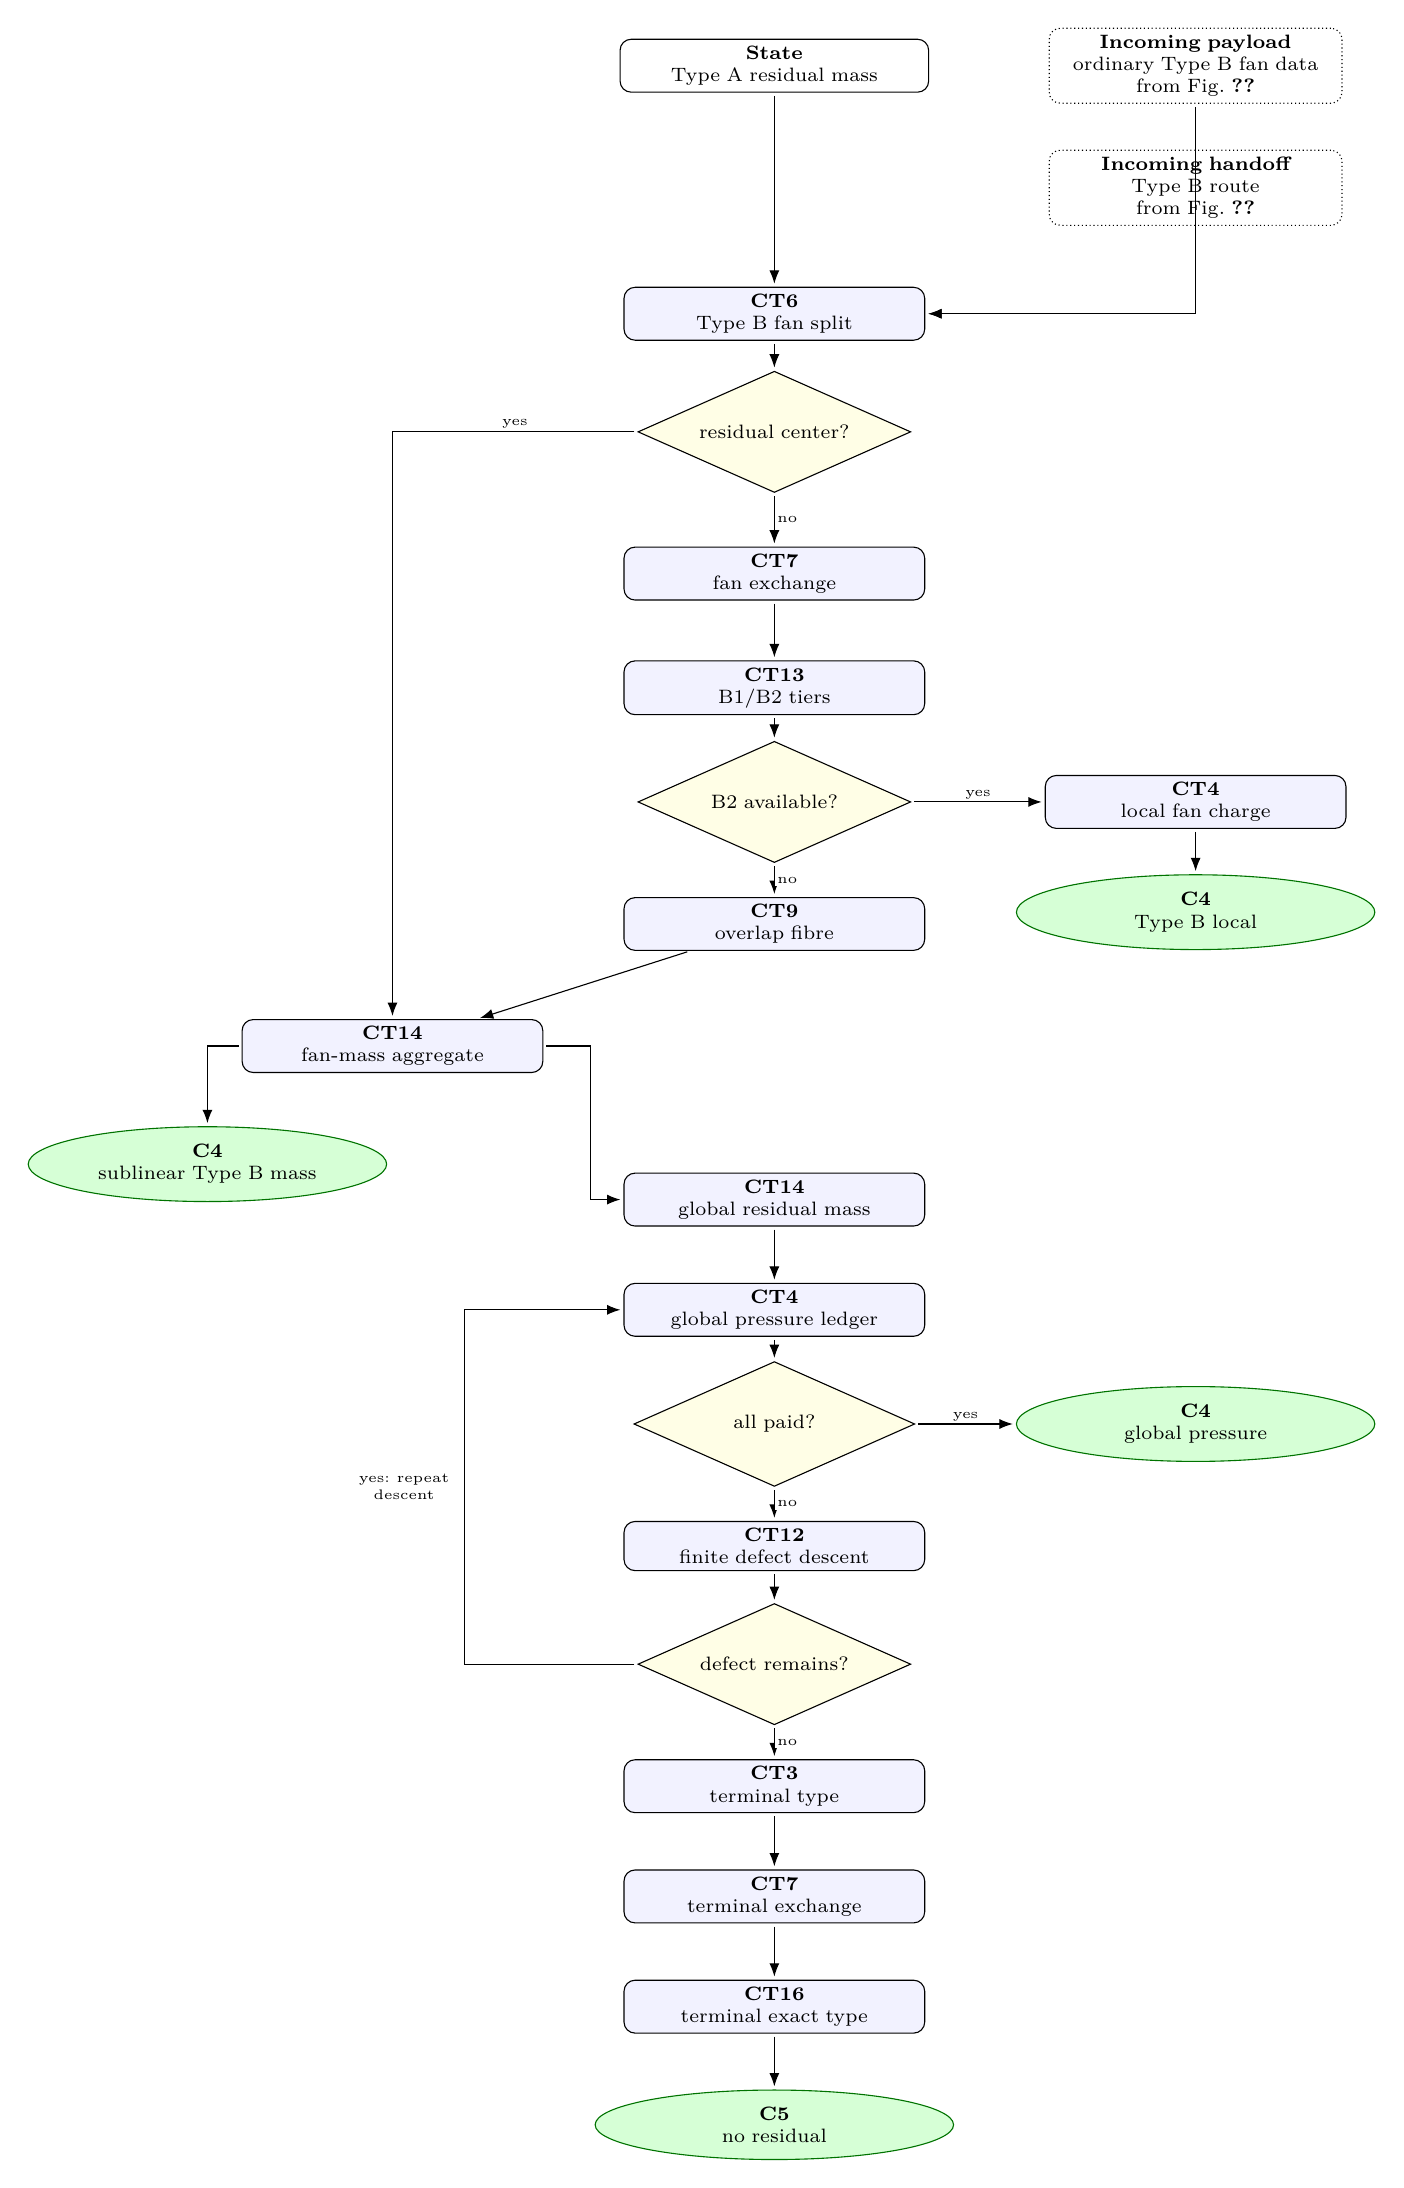
\begin{tikzpicture}[
x=1cm,
y=1cm,
every node/.style={font=\scriptsize},
tactic/.style={rectangle,rounded corners,draw,fill=blue!5,align=center,inner sep=2.4pt,minimum width=3.65cm,text width=3.65cm},
state/.style={rectangle,rounded corners,draw,fill=white,align=center,inner sep=2.4pt,minimum width=3.75cm,text width=3.75cm},
test/.style={diamond,draw,fill=yellow!10,aspect=2.25,align=center,inner sep=1.4pt,minimum width=3.45cm,text width=2.75cm},
close/.style={ellipse,draw=green!45!black,fill=green!16,align=center,inner sep=2.4pt,minimum width=3.05cm,text width=3.05cm},
handoff/.style={rectangle,rounded corners,draw,densely dotted,align=center,inner sep=2.4pt,minimum width=3.55cm,text width=3.55cm},
arr/.style={-{Latex[length=1.7mm]},thin,shorten <=1.1pt,shorten >=1.1pt},
route/.style={-{Latex[length=1.7mm]},thin,shorten <=1.1pt,shorten >=1.1pt},
lbl/.style={font=\tiny,inner sep=0.9pt,fill=white}
]
\node[state] (atype) at (0,1.60) {\textbf{State}\\Type A residual mass};
\node[handoff] (bfan) at (5.35,1.60) {\textbf{Incoming payload}\\ordinary Type B fan data\\from Fig.~\ref{fig:eg-high-level-ct-flow-iv}};
\node[handoff] (broute) at (5.35,0.05) {\textbf{Incoming handoff}\\Type B route\\from Fig.~\ref{fig:eg-high-level-ct-flow-v}};
\node[tactic] (ct6b) at (0,-1.55) {\textbf{CT6}\\Type B fan split};
\node[test] (rescenter) at (0,-3.05) {residual center?};
\node[tactic] (ct7b) at (0,-4.85) {\textbf{CT7}\\fan exchange};
\node[tactic] (ct13b) at (0,-6.30) {\textbf{CT13}\\B1/B2 tiers};
\node[test] (b2) at (0,-7.75) {B2 available?};
\node[tactic] (ct4b) at (5.35,-7.75) {\textbf{CT4}\\local fan charge};
\node[close] (c4b) at (5.35,-9.15) {\textbf{C4}\\Type B local};
\node[tactic] (ct9b) at (0,-9.30) {\textbf{CT9}\\overlap fibre};
\node[tactic] (ct14b) at (-4.85,-10.85) {\textbf{CT14}\\fan-mass aggregate};
\node[close] (c4mass) at (-7.20,-12.35) {\textbf{C4}\\sublinear Type B mass};
\node[tactic] (ct14join) at (0,-12.80) {\textbf{CT14}\\global residual mass};
\node[tactic] (ct4join) at (0,-14.20) {\textbf{CT4}\\global pressure ledger};
\node[test] (paid) at (0,-15.65) {all paid?};
\node[close] (c4global) at (5.35,-15.65) {\textbf{C4}\\global pressure};
\node[tactic] (ct12f) at (0,-17.20) {\textbf{CT12}\\finite defect descent};
\node[test] (defect) at (0,-18.70) {defect remains?};
\node[tactic] (ct3f) at (0,-20.25) {\textbf{CT3}\\terminal type};
\node[tactic] (ct7f) at (0,-21.65) {\textbf{CT7}\\terminal exchange};
\node[tactic] (ct16f) at (0,-23.05) {\textbf{CT16}\\terminal exact type};
\node[close] (c5final) at (0,-24.55) {\textbf{C5}\\no residual};

\draw[route] (bfan) |- (ct6b);
\draw[route] (broute) |- (ct6b);
\draw[arr] (atype) -- (ct6b);
\draw[arr] (ct6b) -- (rescenter);
\draw[arr] (rescenter) -- node[lbl,right]{no} (ct7b);
\draw[arr] (rescenter) -| node[lbl,near start,above]{yes} (ct14b);
\draw[arr] (ct7b) -- (ct13b);
\draw[arr] (ct13b) -- (b2);
\draw[arr] (b2) -- node[lbl,above]{yes} (ct4b);
\draw[arr] (ct4b) -- (c4b);
\draw[arr] (b2) -- node[lbl,right]{no} (ct9b);
\draw[arr] (ct9b) -- (ct14b);
\coordinate (typebmassbend) at (-7.20,-10.85);
\draw[arr] (ct14b.west) -- (typebmassbend) -- (c4mass.north);
\draw[arr] (ct14b.east) -- ++(0.60,0) |- (ct14join.west);
\draw[arr] (ct14join) -- (ct4join);
\draw[arr] (ct4join) -- (paid);
\draw[arr] (paid) -- node[lbl,above]{yes} (c4global);
\draw[arr] (paid) -- node[lbl,right]{no} (ct12f);
\draw[arr] (ct12f) -- (defect);
\draw[arr] (defect.west) -- ++(-2.20,0) |- node[lbl,pos=0.25,left,text width=1.45cm,align=center]{yes: repeat descent} (ct4join.west);
\draw[arr] (defect) -- node[lbl,right]{no} (ct3f);
\draw[arr] (ct3f) -- (ct7f);
\draw[arr] (ct7f) -- (ct16f);
\draw[arr] (ct16f) -- (c5final);
\end{tikzpicture}%
}
\caption[EG high-level CT proof-flow chart VI]{EG high-level CT proof-flow chart VI\@.  The sixth detailed panel joins the Type A residual mass with the Type B fan and handoff payloads, closes the Type B mass, and runs the final pressure and finite-descent closure.}
\label{fig:eg-high-level-ct-flow-vi}
\end{figure}

\iffalse

\begin{figure}[p]
\centering
\resizebox{0.98\textwidth}{!}{%
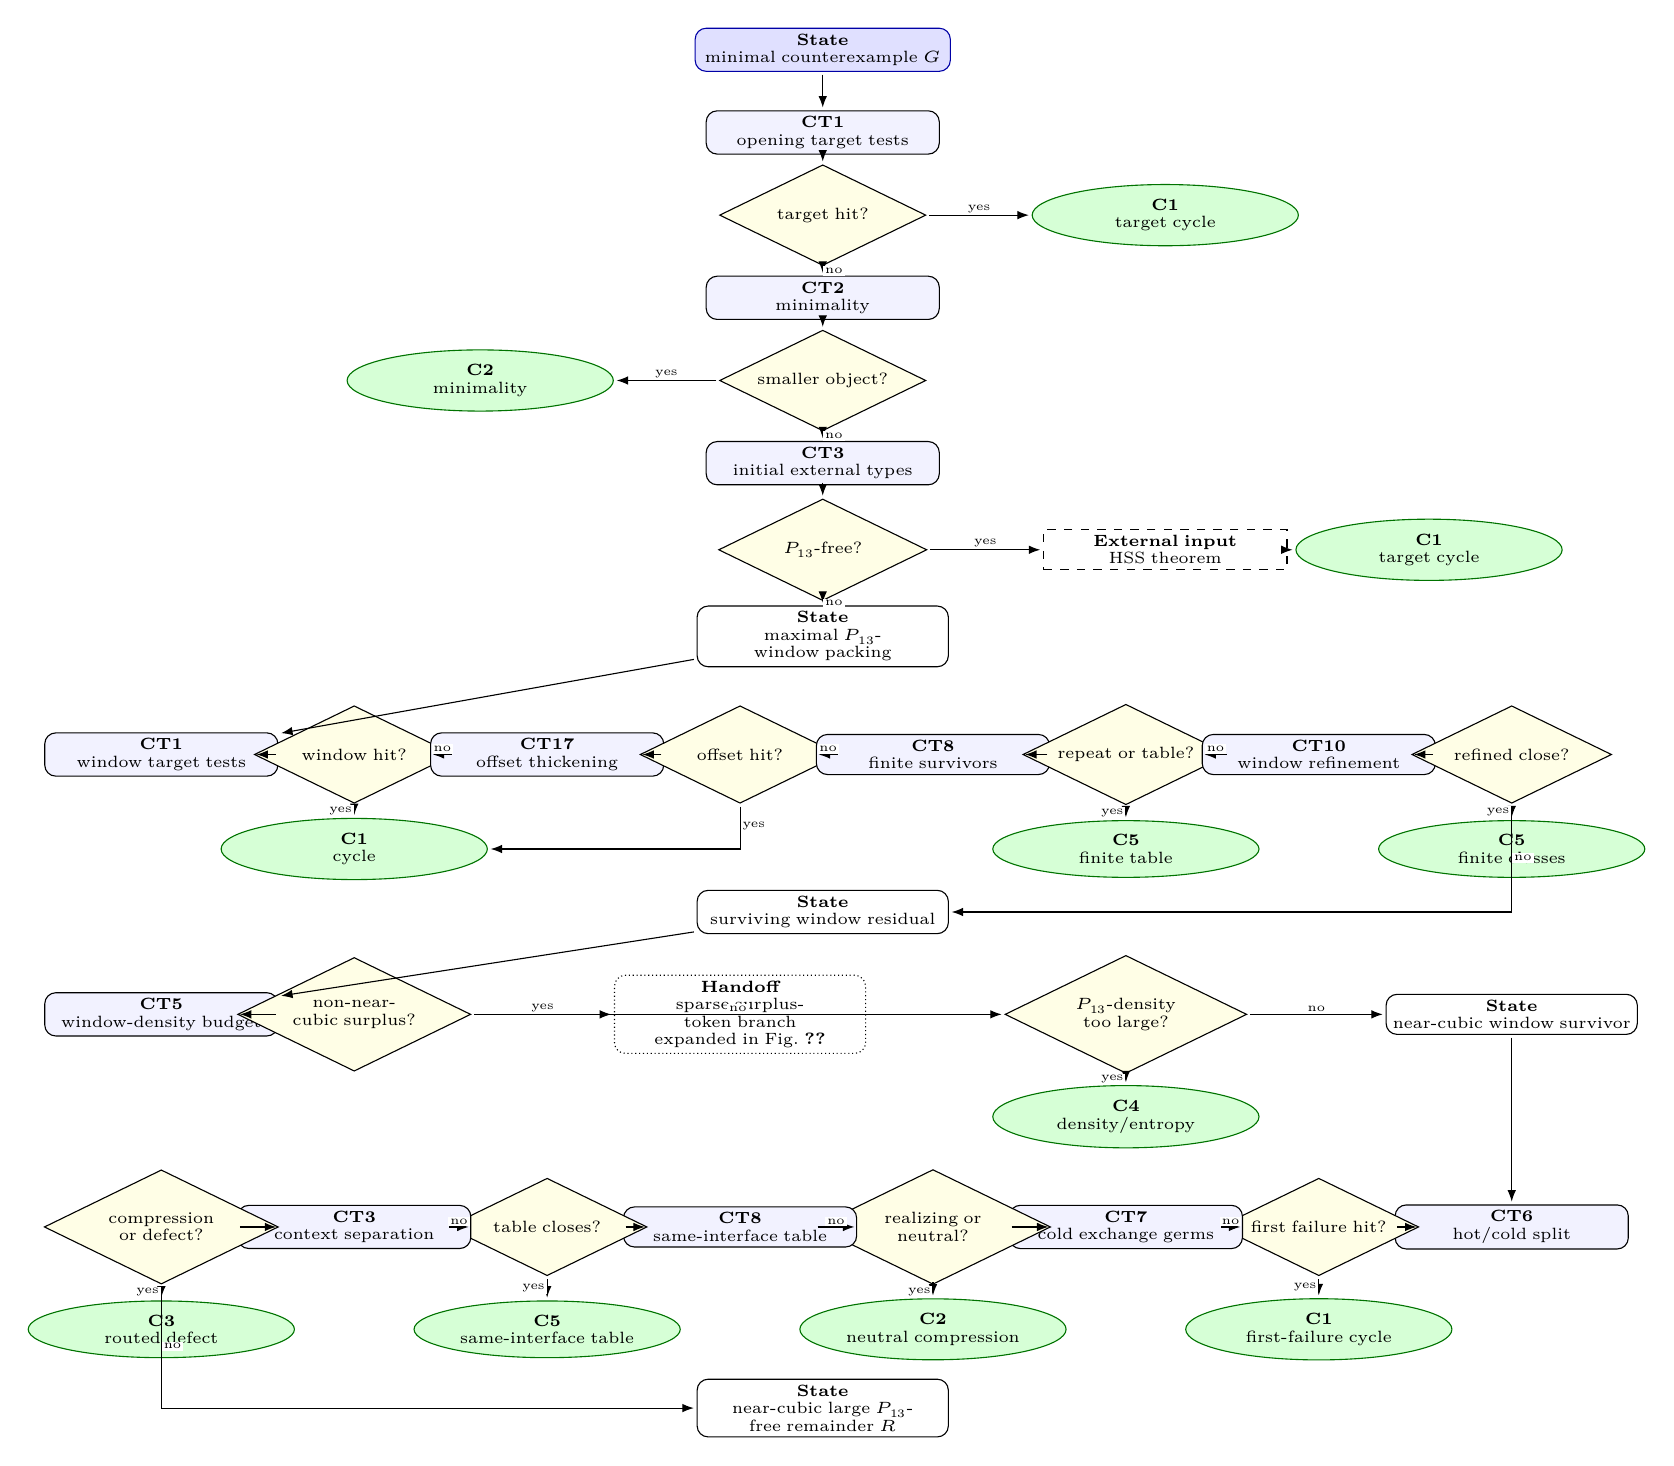
\begin{tikzpicture}[
x=1cm,
y=1cm,
every node/.style={font=\fontsize{5.9}{6.3}\selectfont},
tactic/.style={rectangle,rounded corners,draw,fill=blue!5,align=center,inner sep=2.0pt,minimum width=2.82cm,text width=2.82cm},
setup/.style={rectangle,rounded corners,draw,fill=blue!12,draw=blue!65!black,align=center,inner sep=2.0pt,minimum width=3.10cm,text width=3.10cm},
state/.style={rectangle,rounded corners,draw,fill=white,align=center,inner sep=2.0pt,minimum width=3.05cm,text width=3.05cm},
test/.style={diamond,draw,fill=yellow!10,aspect=2.05,align=center,inner sep=1pt,minimum width=2.50cm,text width=2.02cm},
close/.style={ellipse,draw=green!45!black,fill=green!16,align=center,inner sep=2.0pt,minimum width=2.25cm,text width=2.25cm},
external/.style={rectangle,draw,dashed,align=center,inner sep=2.0pt,minimum width=2.95cm,text width=2.95cm},
handoff/.style={rectangle,rounded corners,draw,densely dotted,align=center,inner sep=2.0pt,minimum width=3.05cm,text width=3.05cm},
arr/.style={-{Latex[length=1.45mm]},thin,shorten <=1.0pt,shorten >=1.0pt},
lbl/.style={font=\fontsize{4.4}{4.8}\selectfont,inner sep=0.7pt,fill=white}
]
\node[setup] (start) at (0,0) {\textbf{State}\\minimal counterexample \(G\)};
\node[tactic] (ct1open) at (0,-1.05) {\textbf{CT1}\\opening target tests};
\node[test] (dopen) at (0,-2.10) {target hit?};
\node[close] (c1open) at (4.35,-2.10) {\textbf{C1}\\target cycle};
\node[tactic] (ct2open) at (0,-3.15) {\textbf{CT2}\\minimality};
\node[test] (dmin) at (0,-4.20) {smaller object?};
\node[close] (c2open) at (-4.35,-4.20) {\textbf{C2}\\minimality};
\node[tactic] (ct3open) at (0,-5.25) {\textbf{CT3}\\initial external types};
\node[test] (dp13) at (0,-6.35) {\(P_{13}\)-free?};
\node[external] (hss) at (4.35,-6.35) {\textbf{External input}\\HSS theorem};
\node[close] (c1hss) at (7.70,-6.35) {\textbf{C1}\\target cycle};
\node[state] (pack) at (0,-7.45) {\textbf{State}\\maximal \(P_{13}\)-window packing};

\node[tactic] (ct1win) at (-8.40,-8.95) {\textbf{CT1}\\window target tests};
\node[test] (dwin) at (-5.95,-8.95) {window hit?};
\node[tactic] (ct17win) at (-3.50,-8.95) {\textbf{CT17}\\offset thickening};
\node[test] (doffset) at (-1.05,-8.95) {offset hit?};
\node[tactic] (ct8win) at (1.40,-8.95) {\textbf{CT8}\\finite survivors};
\node[test] (dpumpwin) at (3.85,-8.95) {repeat or table?};
\node[tactic] (ct10win) at (6.30,-8.95) {\textbf{CT10}\\window refinement};
\node[test] (drefwin) at (8.75,-8.95) {refined close?};
\node[close] (c1win) at (-5.95,-10.15) {\textbf{C1}\\cycle};
\node[close] (c5win) at (3.85,-10.15) {\textbf{C5}\\finite table};
\node[close] (c5ref) at (8.75,-10.15) {\textbf{C5}\\finite classes};
\node[state] (coldstate) at (0,-10.95) {\textbf{State}\\surviving window residual};

\node[tactic] (ct5spine) at (-8.40,-12.25) {\textbf{CT5}\\window-density budget};
\node[test] (dsurplus) at (-5.95,-12.25) {non-near-cubic surplus?};
\node[handoff] (surplusroute) at (-1.05,-12.25) {\textbf{Handoff}\\sparse surplus-token branch\\expanded in Fig.~\ref{fig:eg-high-level-ct-flow-ii}};
\node[test] (ddensity) at (3.85,-12.25) {\(P_{13}\)-density too large?};
\node[close] (cdense) at (3.85,-13.55) {\textbf{C4}\\density/entropy};
\node[state] (spinecold) at (8.75,-12.25) {\textbf{State}\\near-cubic window survivor};

\node[tactic] (ct6cold) at (8.75,-14.95) {\textbf{CT6}\\hot/cold split};
\node[test] (dcold) at (6.30,-14.95) {first failure hit?};
\node[tactic] (ct7cold) at (3.85,-14.95) {\textbf{CT7}\\cold exchange germs};
\node[test] (dexcold) at (1.40,-14.95) {realizing or neutral?};
\node[tactic] (ct8cold) at (-1.05,-14.95) {\textbf{CT8}\\same-interface table};
\node[test] (dtablecold) at (-3.50,-14.95) {table closes?};
\node[tactic] (ct3cold) at (-5.95,-14.95) {\textbf{CT3}\\context separation};
\node[test] (dtypecold) at (-8.40,-14.95) {compression or defect?};
\node[close] (c1cold) at (6.30,-16.25) {\textbf{C1}\\first-failure cycle};
\node[close] (c2cold) at (1.40,-16.25) {\textbf{C2}\\neutral compression};
\node[close] (c5cold) at (-3.50,-16.25) {\textbf{C5}\\same-interface table};
\node[close] (c3cold) at (-8.40,-16.25) {\textbf{C3}\\routed defect};
\node[state] (budgetstate) at (0,-17.25) {\textbf{State}\\near-cubic large \(P_{13}\)-free remainder \(R\)};

\draw[arr] (start) -- (ct1open);
\draw[arr] (ct1open) -- (dopen);
\draw[arr] (dopen) -- node[lbl,above]{yes} (c1open);
\draw[arr] (dopen) -- node[lbl,right]{no} (ct2open);
\draw[arr] (ct2open) -- (dmin);
\draw[arr] (dmin) -- node[lbl,above]{yes} (c2open);
\draw[arr] (dmin) -- node[lbl,right]{no} (ct3open);
\draw[arr] (ct3open) -- (dp13);
\draw[arr] (dp13) -- node[lbl,above]{yes} (hss);
\draw[arr] (hss) -- (c1hss);
\draw[arr] (dp13) -- node[lbl,right]{no} (pack);

\draw[arr] (pack) -- (ct1win);
\draw[arr] (ct1win) -- (dwin);
\draw[arr] (dwin) -- node[lbl,left]{yes} (c1win);
\draw[arr] (dwin) -- node[lbl,above]{no} (ct17win);
\draw[arr] (ct17win) -- (doffset);
\draw[arr] (doffset) |- node[lbl,near start,right]{yes} (c1win);
\draw[arr] (doffset) -- node[lbl,above]{no} (ct8win);
\draw[arr] (ct8win) -- (dpumpwin);
\draw[arr] (dpumpwin) -- node[lbl,left]{yes} (c5win);
\draw[arr] (dpumpwin) -- node[lbl,above]{no} (ct10win);
\draw[arr] (ct10win) -- (drefwin);
\draw[arr] (drefwin) -- node[lbl,left]{yes} (c5ref);
\draw[arr] (drefwin) |- node[lbl,near start,right]{no} (coldstate);

\draw[arr] (coldstate) -- (ct5spine);
\draw[arr] (ct5spine) -- (dsurplus);
\draw[arr] (dsurplus) -- node[lbl,above]{yes} (surplusroute);
\draw[arr] (dsurplus) -- node[lbl,above]{no} (ddensity);
\draw[arr] (ddensity) -- node[lbl,left]{yes} (cdense);
\draw[arr] (ddensity) -- node[lbl,above]{no} (spinecold);
\draw[arr] (spinecold) -- (ct6cold);
\draw[arr] (ct6cold) -- (dcold);
\draw[arr] (dcold) -- node[lbl,left]{yes} (c1cold);
\draw[arr] (dcold) -- node[lbl,above]{no} (ct7cold);
\draw[arr] (ct7cold) -- (dexcold);
\draw[arr] (dexcold) -- node[lbl,left]{yes} (c2cold);
\draw[arr] (dexcold) -- node[lbl,above]{no} (ct8cold);
\draw[arr] (ct8cold) -- (dtablecold);
\draw[arr] (dtablecold) -- node[lbl,left]{yes} (c5cold);
\draw[arr] (dtablecold) -- node[lbl,above]{no} (ct3cold);
\draw[arr] (ct3cold) -- (dtypecold);
\draw[arr] (dtypecold) -- node[lbl,left]{yes} (c3cold);
\draw[arr] (dtypecold) |- node[lbl,near start,right]{no} (budgetstate);
\end{tikzpicture}%
}
\caption[EG high-level CT proof-flow chart I]{EG high-level CT proof-flow chart I.  The first panel starts with the minimal counterexample, runs the opening target, minimality, type, \(P_{13}\)-window, budget-density, and hot/cold CT applications, and ends at the boundary node ``near-cubic large \(P_{13}\)-free remainder \(R\),'' which is repeated as the first node of Fig.~\ref{fig:eg-high-level-ct-flow-ii}.  The non-near-cubic surplus branch is a genuine side continuation and is expanded in Fig.~\ref{fig:eg-high-level-ct-flow-ii}.}
\label{fig:eg-high-level-ct-flow-i}
\end{figure}

\begin{figure}[p]
\centering
\resizebox{\textwidth}{!}{%
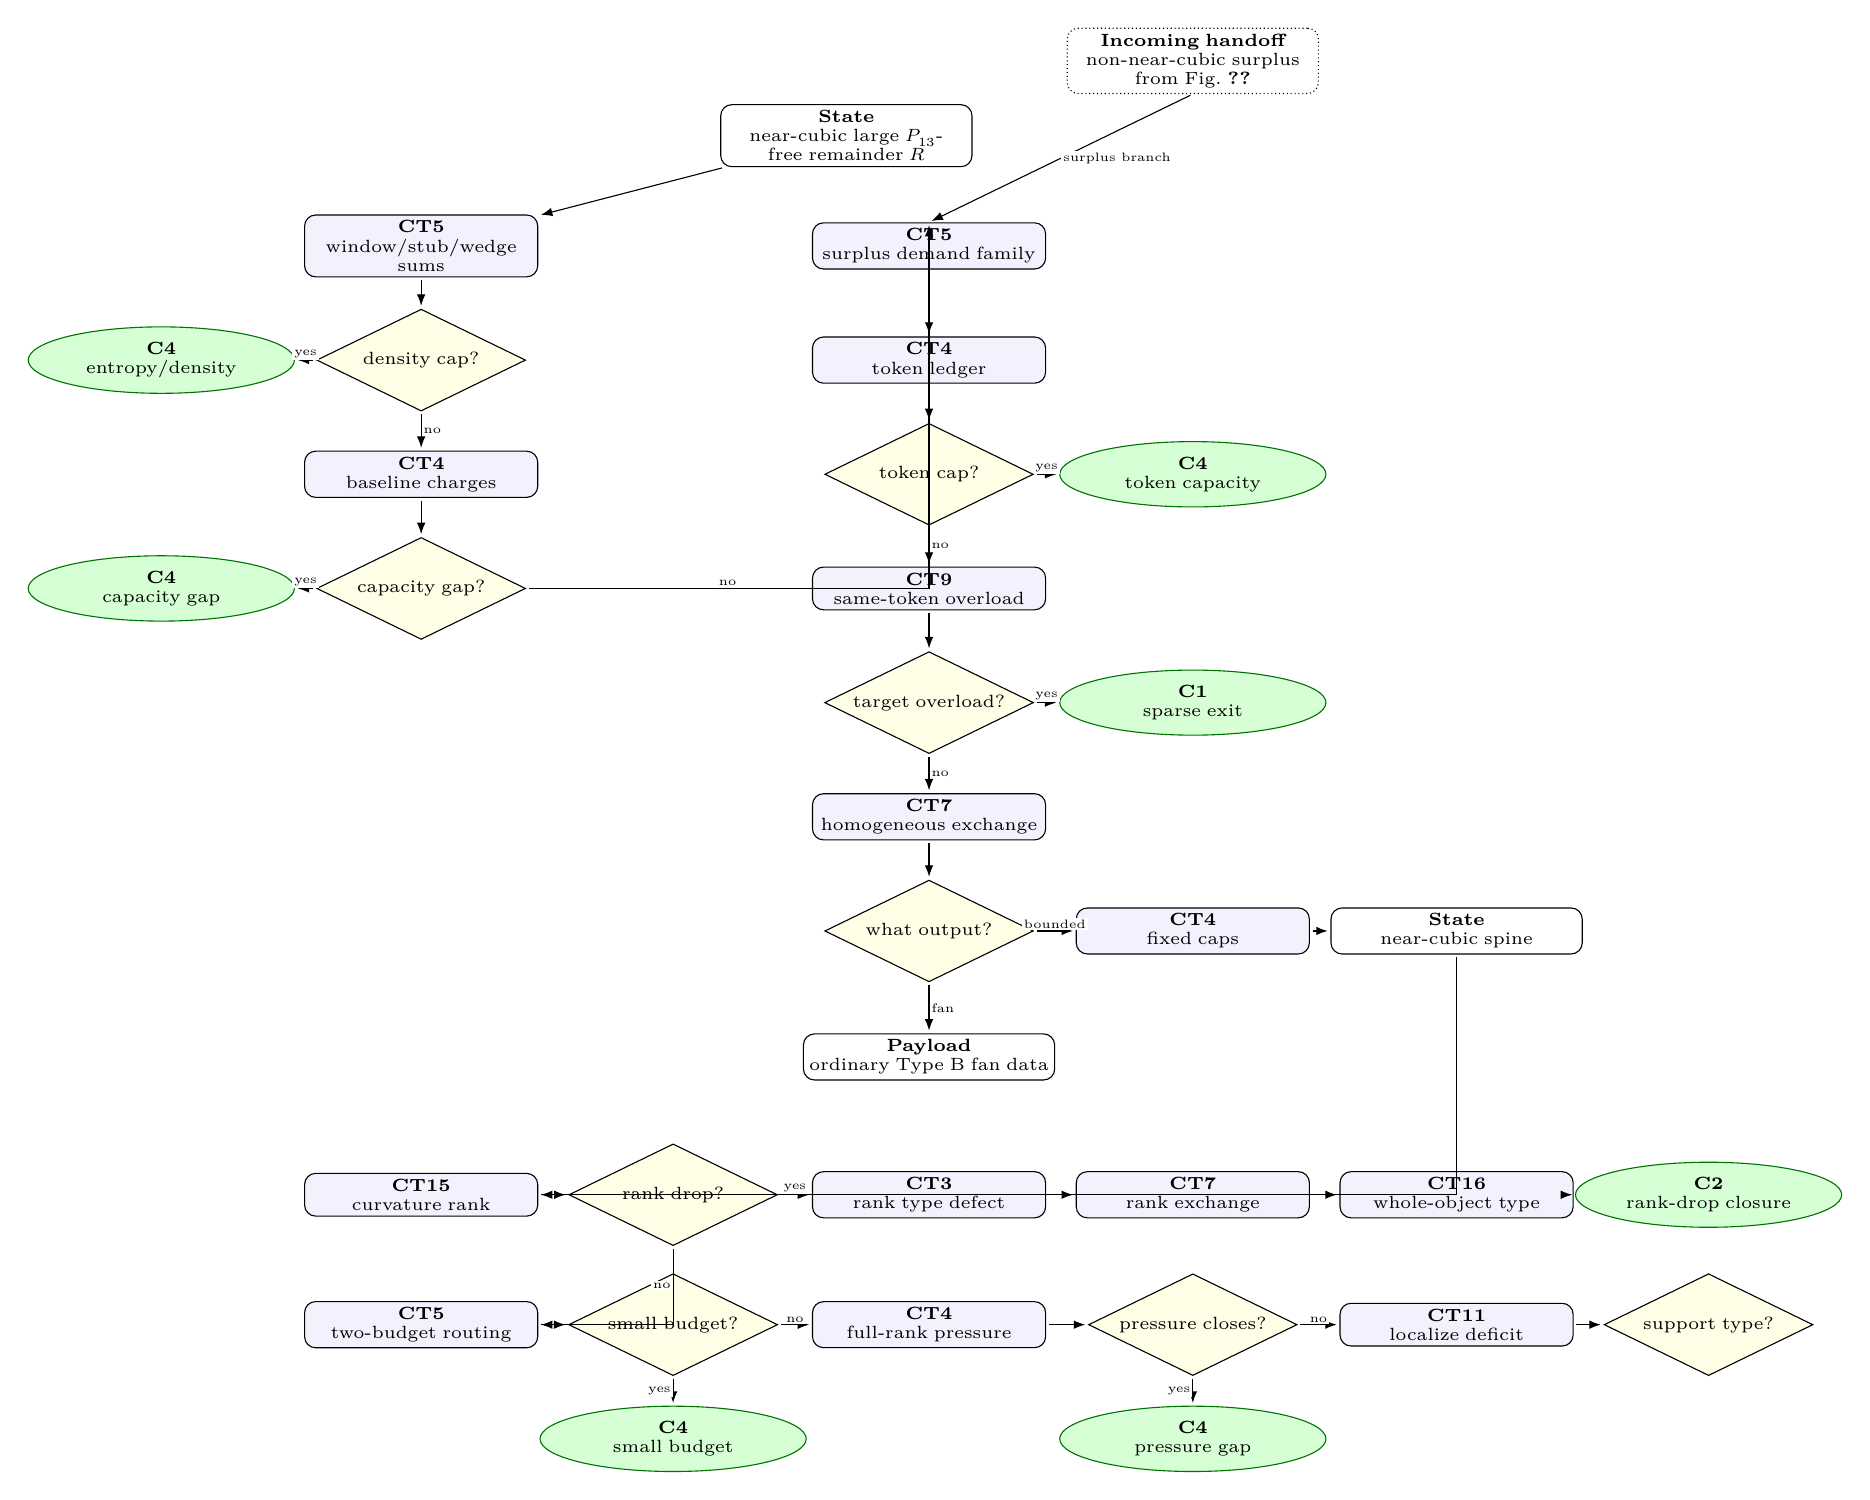
\begin{tikzpicture}[
x=1cm,
y=1cm,
every node/.style={font=\fontsize{6.4}{6.9}\selectfont},
tactic/.style={rectangle,rounded corners,draw,fill=blue!5,align=center,inner sep=2.0pt,minimum width=2.82cm,text width=2.82cm},
state/.style={rectangle,rounded corners,draw,fill=white,align=center,inner sep=2.0pt,minimum width=3.05cm,text width=3.05cm},
handoff/.style={rectangle,rounded corners,draw,densely dotted,align=center,inner sep=2.0pt,minimum width=3.05cm,text width=3.05cm},
test/.style={diamond,draw,fill=yellow!10,aspect=2.05,align=center,inner sep=1pt,minimum width=2.50cm,text width=2.02cm},
close/.style={ellipse,draw=green!45!black,fill=green!16,align=center,inner sep=2.0pt,minimum width=2.25cm,text width=2.25cm},
arr/.style={-{Latex[length=1.45mm]},thin,shorten <=1.0pt,shorten >=1.0pt},
lbl/.style={font=\fontsize{4.4}{4.8}\selectfont,inner sep=0.7pt,fill=white}
]
\node[state] (budgetstate) at (0,0) {\textbf{State}\\near-cubic large \(P_{13}\)-free remainder \(R\)};
\node[handoff] (surplusin) at (4.40,0.95) {\textbf{Incoming handoff}\\non-near-cubic surplus\\from Fig.~\ref{fig:eg-high-level-ct-flow-i}};
\node[tactic] (ct5bud) at (-5.40,-1.40) {\textbf{CT5}\\window/stub/wedge sums};
\node[test] (dbud) at (-5.40,-2.85) {density cap?};
\node[close] (c4bud) at (-8.70,-2.85) {\textbf{C4}\\entropy/density};
\node[tactic] (ct4bud) at (-5.40,-4.30) {\textbf{CT4}\\baseline charges};
\node[test] (dchargebud) at (-5.40,-5.75) {capacity gap?};
\node[close] (c4base) at (-8.70,-5.75) {\textbf{C4}\\capacity gap};

\node[tactic] (ct5surp) at (1.05,-1.40) {\textbf{CT5}\\surplus demand family};
\node[tactic] (ct4surp) at (1.05,-2.85) {\textbf{CT4}\\token ledger};
\node[test] (dsurpcharge) at (1.05,-4.30) {token cap?};
\node[close] (c4tok) at (4.40,-4.30) {\textbf{C4}\\token capacity};
\node[tactic] (ct9surp) at (1.05,-5.75) {\textbf{CT9}\\same-token overload};
\node[test] (dover) at (1.05,-7.20) {target overload?};
\node[close] (c1surp) at (4.40,-7.20) {\textbf{C1}\\sparse exit};
\node[tactic] (ct7surp) at (1.05,-8.65) {\textbf{CT7}\\homogeneous exchange};
\node[test] (dexsurp) at (1.05,-10.10) {what output?};
\node[tactic] (ct4caps) at (4.40,-10.10) {\textbf{CT4}\\fixed caps};
\node[state] (spine) at (7.75,-10.10) {\textbf{State}\\near-cubic spine};
\node[state] (fanpayload) at (1.05,-11.70) {\textbf{Payload}\\ordinary Type B fan data};

\node[tactic] (ct15rank) at (-5.40,-13.45) {\textbf{CT15}\\curvature rank};
\node[test] (drank) at (-2.20,-13.45) {rank drop?};
\node[tactic] (ct3rank) at (1.05,-13.45) {\textbf{CT3}\\rank type defect};
\node[tactic] (ct7rank) at (4.40,-13.45) {\textbf{CT7}\\rank exchange};
\node[tactic] (ct16rank) at (7.75,-13.45) {\textbf{CT16}\\whole-object type};
\node[close] (c2rank) at (10.95,-13.45) {\textbf{C2}\\rank-drop closure};
\node[tactic] (ct5two) at (-5.40,-15.10) {\textbf{CT5}\\two-budget routing};
\node[test] (dtwo) at (-2.20,-15.10) {small budget?};
\node[tactic] (ct4press) at (1.05,-15.10) {\textbf{CT4}\\full-rank pressure};
\node[test] (dpress) at (4.40,-15.10) {pressure closes?};
\node[tactic] (ct11loc) at (7.75,-15.10) {\textbf{CT11}\\localize deficit};
\node[test] (dsplit) at (10.95,-15.10) {support type?};
\node[close] (c4two) at (-2.20,-16.55) {\textbf{C4}\\small budget};
\node[close] (c4press) at (4.40,-16.55) {\textbf{C4}\\pressure gap};

\draw[arr] (budgetstate) -- (ct5bud);
\draw[arr] (ct5bud) -- (dbud);
\draw[arr] (dbud) -- node[lbl,above]{yes} (c4bud);
\draw[arr] (dbud) -- node[lbl,right]{no} (ct4bud);
\draw[arr] (ct4bud) -- (dchargebud);
\draw[arr] (dchargebud) -- node[lbl,above]{yes} (c4base);
\draw[arr] (dchargebud.east) -| node[lbl,near start,above]{no} (ct5surp.north);
\draw[arr] (surplusin.south) -- node[lbl,right]{surplus branch} (ct5surp.north);
\draw[arr] (ct5surp) -- (ct4surp);
\draw[arr] (ct4surp) -- (dsurpcharge);
\draw[arr] (dsurpcharge) -- node[lbl,above]{yes} (c4tok);
\draw[arr] (dsurpcharge) -- node[lbl,right]{no} (ct9surp);
\draw[arr] (ct9surp) -- (dover);
\draw[arr] (dover) -- node[lbl,above]{yes} (c1surp);
\draw[arr] (dover) -- node[lbl,right]{no} (ct7surp);
\draw[arr] (ct7surp) -- (dexsurp);
\draw[arr] (dexsurp) -- node[lbl,right]{fan} (fanpayload);
\draw[arr] (dexsurp) -- node[lbl,above]{bounded} (ct4caps);
\draw[arr] (ct4caps) -- (spine);

\draw[arr] (spine) |- (ct15rank);
\draw[arr] (ct15rank) -- (drank);
\draw[arr] (drank) -- node[lbl,above]{yes} (ct3rank);
\draw[arr] (ct3rank) -- (ct7rank);
\draw[arr] (ct7rank) -- (ct16rank);
\draw[arr] (ct16rank) -- (c2rank);
\draw[arr] (drank) |- node[lbl,near start,left]{no} (ct5two);
\draw[arr] (ct5two) -- (dtwo);
\draw[arr] (dtwo) -- node[lbl,left]{yes} (c4two);
\draw[arr] (dtwo) -- node[lbl,above]{no} (ct4press);
\draw[arr] (ct4press) -- (dpress);
\draw[arr] (dpress) -- node[lbl,left]{yes} (c4press);
\draw[arr] (dpress) -- node[lbl,above]{no} (ct11loc);
\draw[arr] (ct11loc) -- (dsplit);
\end{tikzpicture}%
}
\caption[EG high-level CT proof-flow chart II]{EG high-level CT proof-flow chart II.  The second panel begins with the boundary node ``near-cubic large \(P_{13}\)-free remainder \(R\),'' carries the local-to-global budgets, sparse surplus-token branch, rank forcing, pressure routing, and localization, and ends at the boundary node ``support type?,'' which is repeated as the first node of Fig.~\ref{fig:eg-high-level-ct-flow-iii}.  The non-near-cubic surplus handoff from Fig.~\ref{fig:eg-high-level-ct-flow-i} enters the surplus-token branch directly.  The fan-data payload is displayed because it enters the Type B branch in the next panel.}
\label{fig:eg-high-level-ct-flow-ii}
\end{figure}

\begin{figure}[p]
\centering
\resizebox{\textwidth}{!}{%
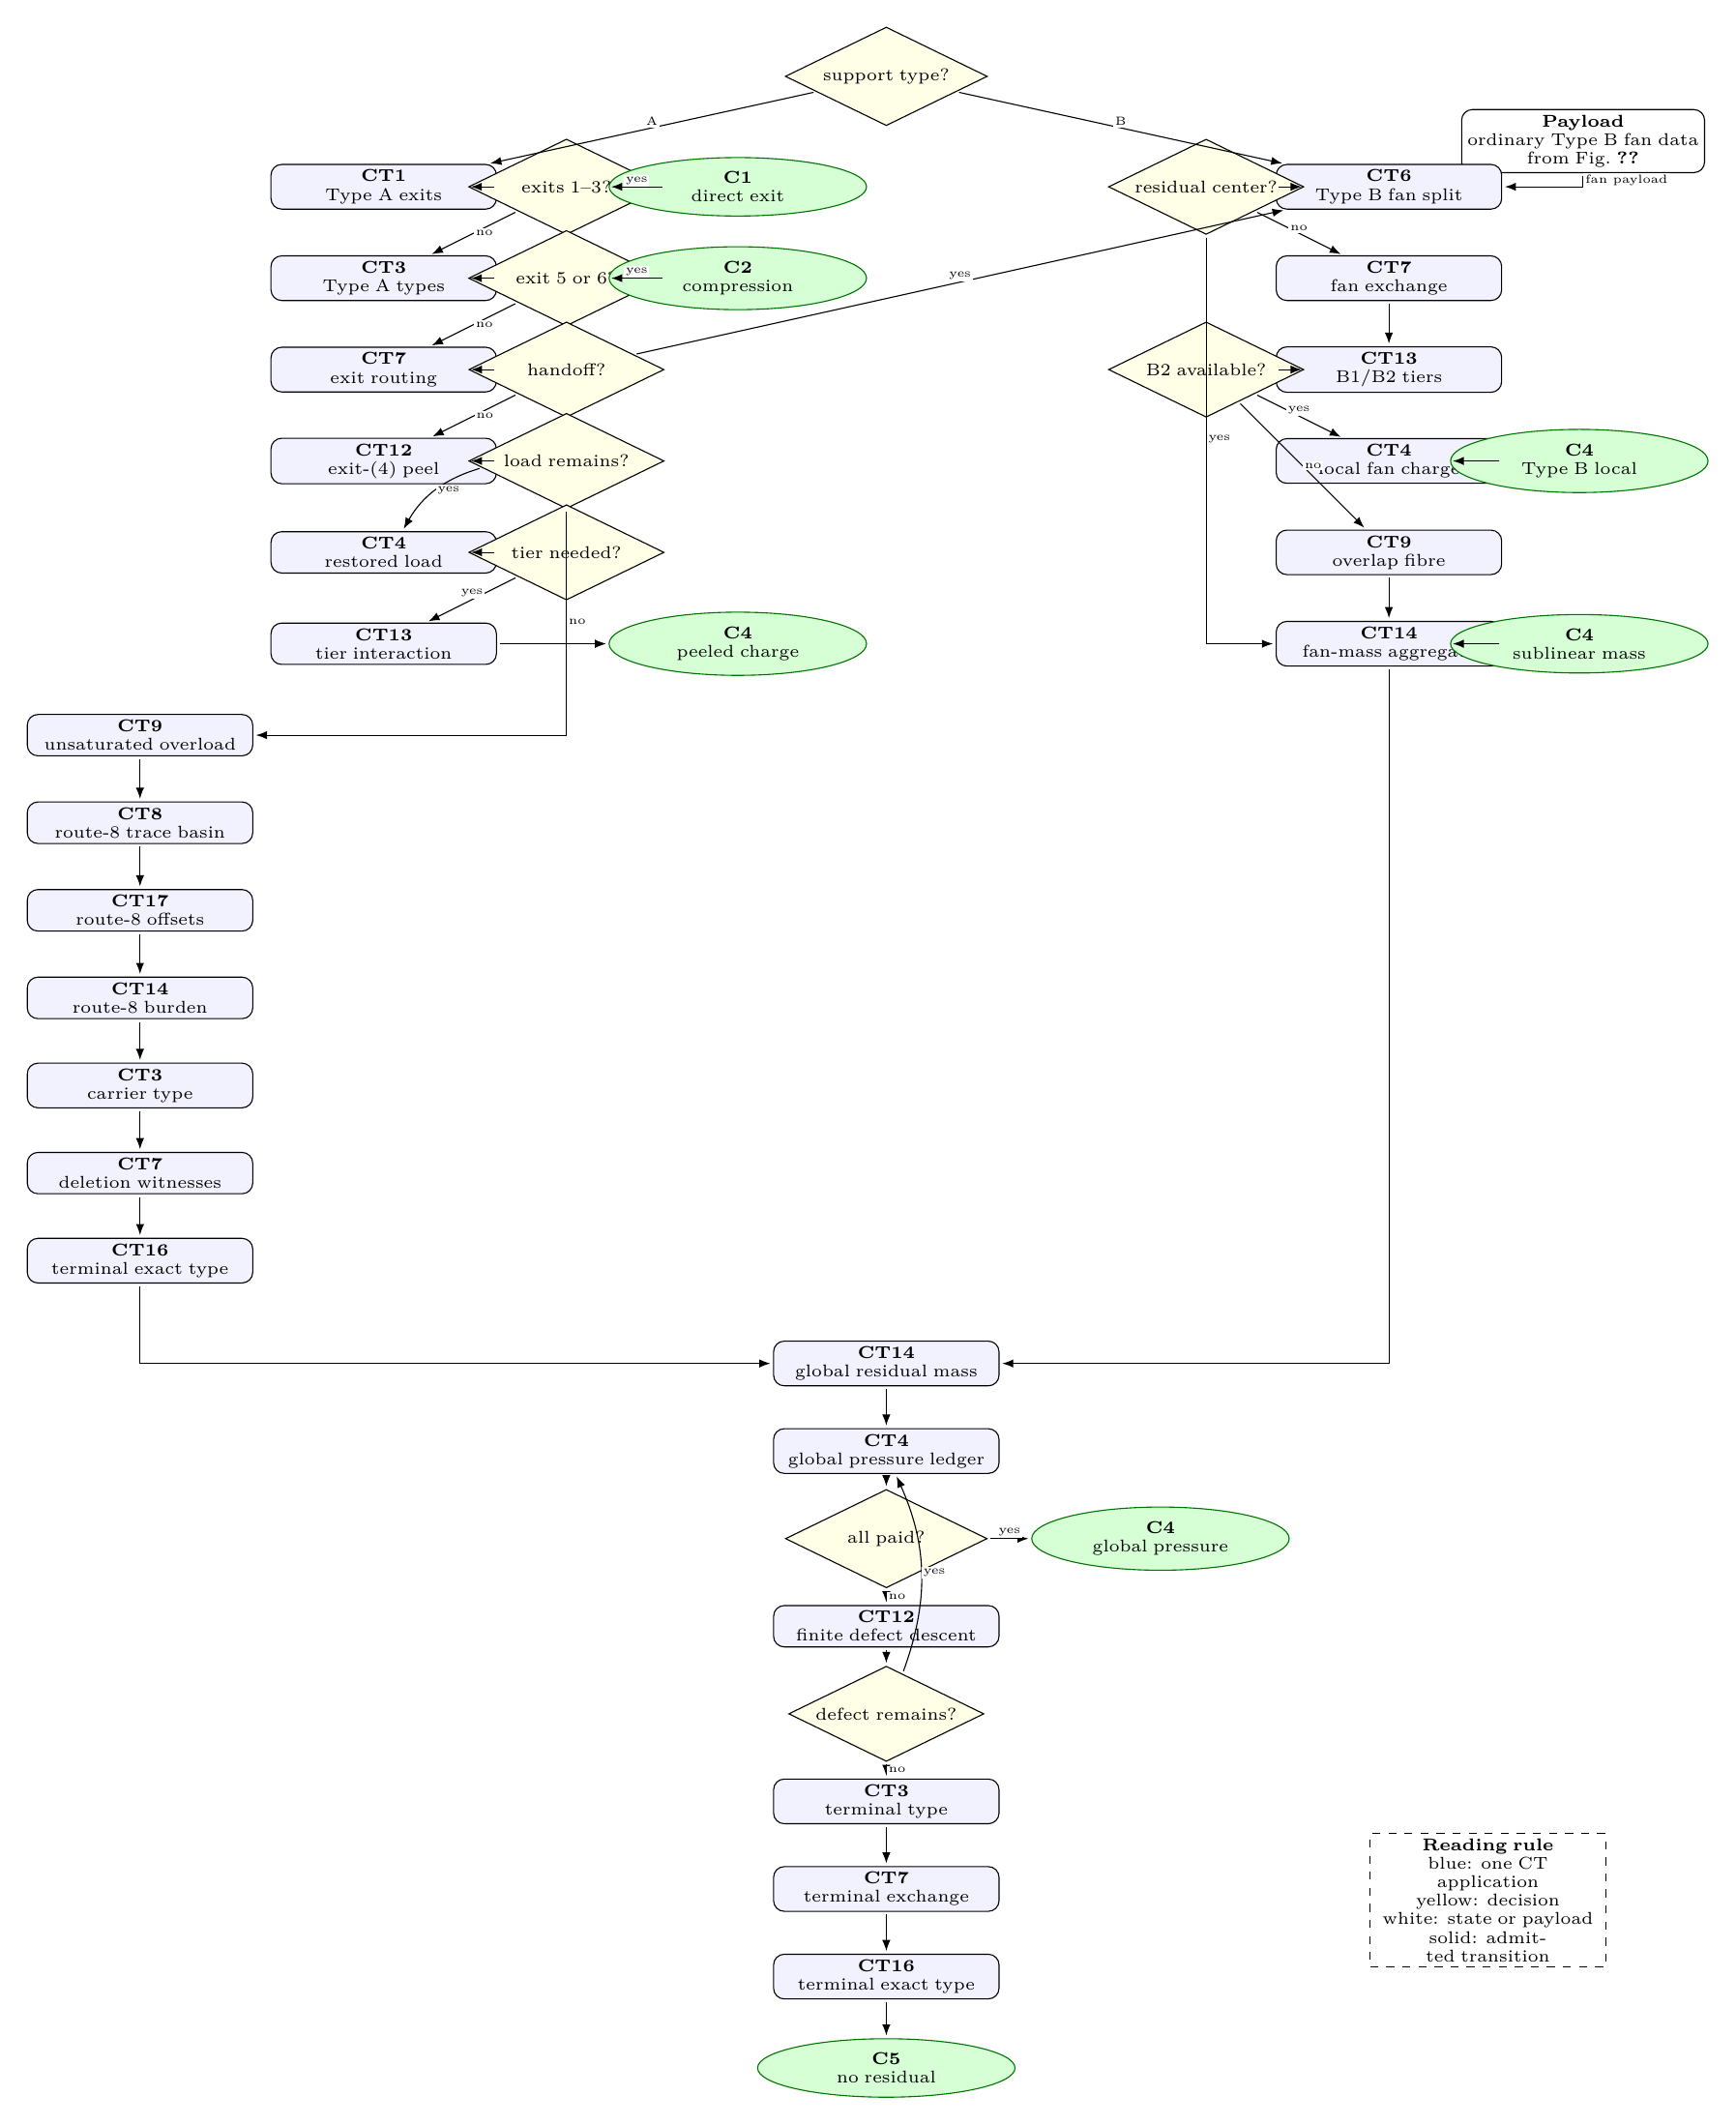
\begin{tikzpicture}[
x=1cm,
y=1cm,
every node/.style={font=\fontsize{6.4}{6.9}\selectfont},
tactic/.style={rectangle,rounded corners,draw,fill=blue!5,align=center,inner sep=2.0pt,minimum width=2.82cm,text width=2.82cm},
state/.style={rectangle,rounded corners,draw,fill=white,align=center,inner sep=2.0pt,minimum width=3.05cm,text width=3.05cm},
test/.style={diamond,draw,fill=yellow!10,aspect=2.05,align=center,inner sep=1pt,minimum width=2.50cm,text width=2.02cm},
close/.style={ellipse,draw=green!45!black,fill=green!16,align=center,inner sep=2.0pt,minimum width=2.25cm,text width=2.25cm},
external/.style={rectangle,draw,dashed,align=center,inner sep=2.0pt,minimum width=2.95cm,text width=2.95cm},
arr/.style={-{Latex[length=1.45mm]},thin,shorten <=1.0pt,shorten >=1.0pt},
route/.style={-{Latex[length=1.45mm]},thin,shorten <=1.0pt,shorten >=1.0pt},
lbl/.style={font=\fontsize{4.4}{4.8}\selectfont,inner sep=0.7pt,fill=white}
]
\node[test] (dsplit) at (0,0) {support type?};
\node[tactic] (ct1a) at (-6.60,-1.45) {\textbf{CT1}\\Type A exits};
\node[test] (da1) at (-4.20,-1.45) {exits 1--3?};
\node[tactic] (ct3a) at (-6.60,-2.65) {\textbf{CT3}\\Type A types};
\node[test] (da3) at (-4.20,-2.65) {exit 5 or 6?};
\node[tactic] (ct7a) at (-6.60,-3.85) {\textbf{CT7}\\exit routing};
\node[test] (da7) at (-4.20,-3.85) {handoff?};
\node[tactic] (ct12a) at (-6.60,-5.05) {\textbf{CT12}\\exit-(4) peel};
\node[test] (da12) at (-4.20,-5.05) {load remains?};
\node[tactic] (ct4a) at (-6.60,-6.25) {\textbf{CT4}\\restored load};
\node[test] (da4) at (-4.20,-6.25) {tier needed?};
\node[tactic] (ct13a) at (-6.60,-7.45) {\textbf{CT13}\\tier interaction};
\node[close] (c1a) at (-1.95,-1.45) {\textbf{C1}\\direct exit};
\node[close] (c2a) at (-1.95,-2.65) {\textbf{C2}\\compression};
\node[close] (c4a) at (-1.95,-7.45) {\textbf{C4}\\peeled charge};

\node[tactic] (ct9a) at (-9.80,-8.65) {\textbf{CT9}\\unsaturated overload};
\node[tactic] (ct8r8) at (-9.80,-9.80) {\textbf{CT8}\\route-8 trace basin};
\node[tactic] (ct17r8) at (-9.80,-10.95) {\textbf{CT17}\\route-8 offsets};
\node[tactic] (ct14r8) at (-9.80,-12.10) {\textbf{CT14}\\route-8 burden};
\node[tactic] (ct3car) at (-9.80,-13.25) {\textbf{CT3}\\carrier type};
\node[tactic] (ct7car) at (-9.80,-14.40) {\textbf{CT7}\\deletion witnesses};
\node[tactic] (ct16car) at (-9.80,-15.55) {\textbf{CT16}\\terminal exact type};

\node[state] (fanpayload) at (9.15,-0.85) {\textbf{Payload}\\ordinary Type B fan data\\from Fig.~\ref{fig:eg-high-level-ct-flow-ii}};
\node[tactic] (ct6b) at (6.60,-1.45) {\textbf{CT6}\\Type B fan split};
\node[test] (db6) at (4.20,-1.45) {residual center?};
\node[tactic] (ct7b) at (6.60,-2.65) {\textbf{CT7}\\fan exchange};
\node[tactic] (ct13b) at (6.60,-3.85) {\textbf{CT13}\\B1/B2 tiers};
\node[test] (db13) at (4.20,-3.85) {B2 available?};
\node[tactic] (ct4b) at (6.60,-5.05) {\textbf{CT4}\\local fan charge};
\node[close] (c4b) at (9.10,-5.05) {\textbf{C4}\\Type B local};
\node[tactic] (ct9b) at (6.60,-6.25) {\textbf{CT9}\\overlap fibre};
\node[tactic] (ct14b) at (6.60,-7.45) {\textbf{CT14}\\fan-mass aggregate};
\node[close] (c4bfan) at (9.10,-7.45) {\textbf{C4}\\sublinear mass};

\node[tactic] (ct14join) at (0,-16.90) {\textbf{CT14}\\global residual mass};
\node[tactic] (ct4join) at (0,-18.05) {\textbf{CT4}\\global pressure ledger};
\node[test] (djoin) at (0,-19.20) {all paid?};
\node[tactic] (ct12final) at (0,-20.35) {\textbf{CT12}\\finite defect descent};
\node[test] (dfinalpeel) at (0,-21.50) {defect remains?};
\node[tactic] (ct3final) at (0,-22.65) {\textbf{CT3}\\terminal type};
\node[tactic] (ct7final) at (0,-23.80) {\textbf{CT7}\\terminal exchange};
\node[tactic] (ct16final) at (0,-24.95) {\textbf{CT16}\\terminal exact type};
\node[close] (cfinal) at (0,-26.15) {\textbf{C5}\\no residual};
\node[close] (c4join) at (3.60,-19.20) {\textbf{C4}\\global pressure};
\node[external] (legend) at (7.90,-23.95) {\textbf{Reading rule}\\blue: one CT application\\yellow: decision\\white: state or payload\\solid: admitted transition};

\draw[arr] (dsplit) -- node[lbl,above]{A} (ct1a);
\draw[arr] (ct1a) -- (da1);
\draw[arr] (da1) -- node[lbl,above]{yes} (c1a);
\draw[arr] (da1) -- node[lbl,right]{no} (ct3a);
\draw[arr] (ct3a) -- (da3);
\draw[arr] (da3) -- node[lbl,above]{yes} (c2a);
\draw[arr] (da3) -- node[lbl,right]{no} (ct7a);
\draw[arr] (ct7a) -- (da7);
\draw[route] (da7) -- node[lbl,above]{yes} (ct6b);
\draw[arr] (da7) -- node[lbl,right]{no} (ct12a);
\draw[arr] (ct12a) -- (da12);
\draw[arr] (da12) to[bend right=22] node[lbl,right]{yes} (ct4a);
\draw[arr] (da12) |- node[lbl,near start,right]{no} (ct9a);
\draw[arr] (ct4a) -- (da4);
\draw[arr] (da4) -- node[lbl,above]{yes} (ct13a);
\draw[arr] (da4) |- node[lbl,near start,right]{no} (c4a);
\draw[arr] (ct13a) -- (c4a);
\draw[arr] (ct9a) -- (ct8r8);
\draw[arr] (ct8r8) -- (ct17r8);
\draw[arr] (ct17r8) -- (ct14r8);
\draw[arr] (ct14r8) -- (ct3car);
\draw[arr] (ct3car) -- (ct7car);
\draw[arr] (ct7car) -- (ct16car);

\draw[arr] (dsplit) -- node[lbl,above]{B} (ct6b);
\draw[route] (fanpayload) |- node[lbl,near start,right]{fan payload} (ct6b);
\draw[arr] (ct6b) -- (db6);
\draw[arr] (db6) -- node[lbl,above]{no} (ct7b);
\draw[arr] (db6) |- node[lbl,near start,right]{yes} (ct14b);
\draw[arr] (ct7b) -- (ct13b);
\draw[arr] (ct13b) -- (db13);
\draw[arr] (db13) -- node[lbl,above]{yes} (ct4b);
\draw[arr] (ct4b) -- (c4b);
\draw[arr] (db13) -- node[lbl,right]{no} (ct9b);
\draw[arr] (ct9b) -- (ct14b);
\draw[arr] (ct14b) -- (c4bfan);

\draw[arr] (ct16car) |- (ct14join);
\draw[arr] (ct14b) |- (ct14join);
\draw[arr] (ct14join) -- (ct4join);
\draw[arr] (ct4join) -- (djoin);
\draw[arr] (djoin) -- node[lbl,above]{yes} (c4join);
\draw[arr] (djoin) -- node[lbl,right]{no} (ct12final);
\draw[arr] (ct12final) -- (dfinalpeel);
\draw[arr] (dfinalpeel) to[bend right=22] node[lbl,right]{yes} (ct4join);
\draw[arr] (dfinalpeel) -- node[lbl,right]{no} (ct3final);
\draw[arr] (ct3final) -- (ct7final);
\draw[arr] (ct7final) -- (ct16final);
\draw[arr] (ct16final) -- (cfinal);
\end{tikzpicture}%
}
\caption[EG high-level CT proof-flow chart III]{EG high-level CT proof-flow chart III.  The third panel begins with the boundary decision ``support type?,'' then runs the Type A branch, the Type B branch, the route-8 carrier branch, and the final pressure/descent closure CT by CT.  The fan-data payload from Fig.~\ref{fig:eg-high-level-ct-flow-ii} enters the Type B branch by an admitted typed handoff.}
\label{fig:eg-high-level-ct-flow-iii}
\end{figure}

\fi

\subsection[Advanced patterns in EG]{Advanced patterns in {[}EG{]} keyed to
\texorpdfstring{\secref{advanced-closure-patterns}}{advanced closure patterns}}\label{b.3-advanced-patterns-section-17-in-cc}

\begin{longtable}[]{@{}
  >{\raggedright\arraybackslash}p{(\columnwidth - 2\tabcolsep) * \real{0.5000}}
  >{\raggedright\arraybackslash}p{(\columnwidth - 2\tabcolsep) * \real{0.5000}}@{}}
\toprule\noalign{}
\begin{minipage}[b]{\linewidth}\raggedright
Pattern (this document)
\end{minipage} & \begin{minipage}[b]{\linewidth}\raggedright
Instantiation in {[}EG{]}
\end{minipage} \\
\midrule\noalign{}
\endhead
\bottomrule\noalign{}
\endlastfoot
\secref{peeling-loops-closure-by-well-founded-recursion} Peeling loops & Exit-(4) peeling: the target-defect route peels
exactly one routed load and returns to the saturated-receiver test with
the residual load \(L_4\) (diagram nodes {[}102{]}→{[}89{]});
termination measure = the routed load. \\
\secref{tiered-charging-scheme-failure-as-a-demand} Tiered charging & The Type B ledgers: the hybrid B1 incidence
payment (tier 1) is conditional on the B2 disjointness ledger; B2
failure produces the \emph{minimal Type B overlap obstruction}, charged
to the fan-mass scheme (tier 2) at its assigned surplus units. \\
\secref{aggregate-closure-mass-bounds-on-residual-classes} Aggregate closure & prop:typeB-bridge-sublinear +
thm:large-budget-route8-only: Type B bridge residuals are handled
aggregately; their total negative net charge is bounded by the global
surplus budget \(\sigma(G)=O(\sqrt n)\), hence \(o(|R|)\), while the
branch state forces a linear deficit --- so the class is empty on the
surviving route. \\
\secref{branch-sequencing-and-derived-normalizations} Branch sequencing; derived normalizations; spine & The near-cubic
spine (def:near-cubic-spine) is derived by
prop:nonnear-cubic-sharp-overload-routing, which exhausts the sparse
surplus-token branch before any normalized skeleton budget
\(B_{\rm skel}=\frac32 n\log_2 n+o(n\log n)\) is invoked; every later
estimate names the spine branch on which it is valid. \\
\secref{rank-forcing-charge-only-independent-coordinates} Rank forcing & {[}EG{]} §10: raw curvature tests pass through rank
forcing before entropy charging; a rank drop is routed to
defect/compression/delocalization (lem:curvature-dependence-routing),
and only the full-rank branch (lem:full-rank) pays the forced cost
\(c_\Omega W_2(R)\) into the two-budget routing of {[}EG{]} §11. \\
\secref{the-whole-object-piece-exact-types-under-context-degeneracy} Whole-object piece; exact closed types &
lem:no-silent-global-smearing with the exact response profiles of
{[}EG{]} §10: at \(Z=G\) identifications require literal equality of
closed profiles. \\
\secref{typed-handoffs-between-branches} Typed handoffs & Exit (7): the Type A branch hands \emph{decorated
Type B fan data} to the Type B branch (nodes {[}108{]}→{[}65{]}, typed
input {[}66{]}); the Type B opening hypothesis is exactly that decorated
package. The sparse branch's ``ordinary decorated Type B fan data''
route is a second instance. \\
\secref{black-box-isolation-of-external-inputs} Black-box isolation & The Hegde--Sandeep--Shashank \(P_{13}\)-free
theorem (thm:p13free) is the single load-bearing external input, stated
once in {[}EG{]} §5 and listed under ``External inputs (black boxes)''
in the constraint ledger. \\
\secref{target-thickening-bounded-offsets-against-sparse-targets} Target thickening & {[}EG{]} §7: the window offset set
\(\{0,\dots,12\}\) smears each self-return length \(\ell\) into the
block \([\ell,\ell+12]\); only 10 of the first 39 lengths dodge
\(\{4,8,16,32\}\); at large increments the doubling-orbit criterion
\(\operatorname{ord}_\delta(2)>\delta-13\) forces a hit, and the
surviving small-orbit cases become periodic carriers (G2/G3). \\
\secref{constant-interlock-and-computational-certificates} Constant interlock; computational certificates & {[}EG{]} §1: the
standing constants table (\(c_\Omega\), \(c_{13}\),
\(\theta_{\rm win}\), \(\theta_{\rm high}\), \(\omega\), \(K\),
\(\tau_{\rm win}\), \(\Theta(n)\)), each established at a cited place
and reproduced by the code of the finite-curvature-enumeration appendix;
the thresholds \(\tau(\theta)<1/4\) and \(\tau(\theta)<3/13\) (⇔
\(\theta<1/73\), \(\theta<1/78\)) are the recorded interlock of the
large-budget layer and the hot/cold branch. \\
\secref{proof-engineering-artifacts} Proof-engineering artifacts & {[}EG{]} §1 in full: the
eleven-part numbered dependency diagram (nodes {[}1{]}--{[}157{]}); the
detailed dependency table (node ranges → lemma clusters); the constraint
ledger of numbered invariants in blocks I--VII; the per-lemma invariant
requirements with stage legend; and the invariant → lemma reverse index
for impact analysis. \\
\secref{redundant-closures-and-graceful-degradation} Redundant closures; resilience & {[}EG{]} §0, ``Redundancy and
checkability'': the entropy cap, the curvature-rank squeeze, and the
net-charge collision are arithmetically distinct closures; the
resilience appendix (``Proof resilience: residual counterexamples under
lemma failure'') is the resilience register. Its rows instantiate the
degradation invariant: a failed branch closure yields the named
reduction theorem excluding precisely the corresponding residual class,
with the cold-branch residual serving as the public model for this
reduction semantics during incremental verification. \\
\secref{the-defect-register-recording-discovered-failures} Defect register & {[}EG{]}'s audit history is the model
instance: named defect families are recorded by affected nodes, blast
radius, append-only repair history, and status, and recurring classes are
promoted into the \secref{advanced-closure-patterns} pattern library when they expose a
reusable closure shape. \\
\end{longtable}

\subsection{Reading order}\label{b.4-reading-order}

For a reader new to both documents, \appref{appendix-c.-a-small-worked-instantiation} is the natural starting
point: it gives the full pipeline on a short theorem, including two
audited failed proposals. The suggested sequence is then
\secref{motivation-and-literature-background} and the opening vocabulary
of \secref{scope-and-philosophy} → {[}EG{]} §0 (Architecture) →
\secref{part-ii-the-tactic-library} with the CT inventory and interlock
diagram open → {[}EG{]} §1 (overview, diagrams, and ledgers) →
\secrange{runtime-model}{filling-the-templates} for policy →
\secrange{constant-interlock-and-computational-certificates}{limitations}
for assurance.  The CT
instantiation map in \appref{b.2-closure-tactic-instantiation-map} should be read beside the
corresponding {[}EG{]} chapters; the advanced-pattern map in
\appref{b.3-advanced-patterns-section-17-in-cc} gives the section-level
crosswalk. The cold-branch quantitative case
ledger in {[}EG{]} §7 is recommended as the first full branch to verify
end-to-end: it is short, fully quantitative, and exercises the
active/dormant dichotomy (\secref{the-activedormant-dichotomy}), the exchange trichotomy (\secref{the-exchange-trichotomy}), target
thickening (\secref{target-thickening-bounded-offsets-against-sparse-targets}), and the exhaustive-table closure format (\secref{the-branch-table}) in a
single self-contained unit.

\section{A small worked
instantiation}\label{appendix-c.-a-small-worked-instantiation}

This appendix runs the full pipeline on a theorem short enough to verify
in one sitting. Its purpose is mechanical transparency rather than
mathematical depth. Every main artifact of the method appears in
miniature, and two deliberately failed proposals are included to show
the audits rejecting them. The target set here is the even numbers, a
single residue class modulo \(2\); it is the degenerate shadow of the
sparse target \(\{2^k\}\) in the Erdős--Gyárfás instantiation.

The proof trace below records the same argument in the tactic-invocation
format used by the library. The later subsections supply the
mathematical details behind each row.

\begingroup
\scriptsize
\setlength{\tabcolsep}{1.8pt}
\begin{longtable}[]{@{}
  >{\raggedright\arraybackslash}p{0.06\linewidth}
  >{\raggedright\arraybackslash}p{0.10\linewidth}
  >{\raggedright\arraybackslash}p{0.25\linewidth}
  >{\raggedright\arraybackslash}p{0.22\linewidth}
  >{\raggedright\arraybackslash}p{0.16\linewidth}
  >{\raggedright\arraybackslash}p{0.15\linewidth}@{}}
\toprule\noalign{}
Step & Tactic & Trigger data & Parameters & Outcome & Emitted \\
\midrule\noalign{}
\endhead
\bottomrule\noalign{}
\endlastfoot
1 & CT1 & Target predicate ``even cycle'' and parity-theta tests. & Local test family \(T_{x,y}\). & Test equivalence. & Target-avoiding state. \\
2 & CT2 & Heavy edge \(uv\) with \(d(u),d(v)\ge4\). & Lexicographic size order \((|V|,|E|)\). & C2. & Invariant I1. \\
3 & CT12, rejected & Proposed peel \(\mu=|V_{\ge4}|\) by deleting a high-degree incident edge. & Candidate loop move. & S-Rest fails: the move can break \(\delta\ge3\). & No tactic output; I1 remains. \\
4 & CT6 & Maximum path \(P\) and endpoint \(v\). & Measure \(|P|\). & Residual branch. & I2: \(N(v)\subseteq P\). \\
5 & Global shortcut, rejected & Cycle-space parity argument. & None. & Certificate check fails: no realized local test. & No C-certificate. \\
6 & CT9 & Three endpoint-neighbour positions and two parity labels. & Capacity \(1\) per parity class. & Overload. & Same-parity pair. \\
7 & CT1 & Parity theta at the monochromatic pair. & Two internally disjoint paths. & C1. & Even cycle. \\
\end{longtable}
\endgroup

In the worksheets below, ``parameter-synthesis rule'' refers to
\secref{parameter-synthesis}.

\paragraph{Worksheet CT2-1.}
\begingroup
\small
\begin{verbatim}
Instance:      CT2-1       Branch node: [2]
Input payload: <minimal G; heavy edge uv with d(u),d(v) >= 4>
               emitted by: opening script after CT1-1
Parameters:    slot (1) size order := (|V|,|E|)
               synthesized by parameter-synthesis rule
               slot (2) deletion move := delete uv
               inventory item: minimality
Obligations:   definition<piece uv, deletion> := Lemma C.2, proved
               dichotomy<delta preserved> := degree check, proved
               composition<smaller object> := lexicographic order, proved
Outcome:       C2, deletion-minimality variant
Artifacts:     branch-table row 2; invariant I1:
               every edge has a degree-3 endpoint
Open items:    none
\end{verbatim}
\endgroup

\paragraph{Worksheet CT9-1.}
\begingroup
\small
\begin{verbatim}
Instance:      CT9-1       Branch node: [6]
Input payload: <demands {p1,p2,p3};
               payers = parity classes; capacity C = 1>
               emitted by: CT6-1
Parameters:    slot (1) label map := position mod 2
               synthesized by parameter-synthesis rule
               slot (2) extraction target := pair
               synthesized by parameter-synthesis rule
Obligations:   dichotomy<3 demands, 2 classes> := pigeonhole, proved
               routing<pair payload> := positions distinct, proved
               trigger<pair -> CT1> := Lemma C.6, proved
Outcome:       emitted <parity theta at (x_i,x_j)> -> CT1-2
Artifacts:     branch-table row 6; no slack consumed
Open items:    none
\end{verbatim}
\endgroup

\paragraph{Reject rows.}
Step 3 is an \((E)\)-reject for CT12-1/S-Rest: the proposed edge deletion
does not restore the standing minimum-degree branch state, so no CT12
output is produced. Step 5 is a certificate reject: the cycle-space
parity argument produces an even-cardinality cycle-space element rather
than a realized local test, so it is not C1 and emits no payload. Both
rejections remain in the defect register rather than in the proof flow.

\textbf{Theorem C.} \emph{Every finite graph with minimum degree at
least \(3\) contains a cycle of even length.}

The bound is sharp: odd cycles \(C_{2k+1}\) have minimum degree \(2\)
and no even cycle. This sharpness certificate reappears in \appref{c.6-the-leaf-overload-monochromatic-pair-direct-hit}
as the solved crossover of the rate computation.

\subsection{Target predicate and local
tests}\label{c.1-target-predicate-and-local-tests}

The target predicate is

\[
T(G)=1
\quad\Longleftrightarrow\quad
G\text{ contains an even cycle}.
\]

For distinct vertices \(x\) and \(y\), the \textbf{parity theta}
\(T_{x,y}\) is realized when \(G\) contains two internally disjoint
\(x\)-\(y\) paths whose lengths have the same parity.

\textbf{Lemma C.1 (test equivalence).} \(T(G)\) holds if and only if
some parity theta is realized.

\emph{Proof.} Two internally disjoint \(x\)-\(y\) paths of lengths \(p\)
and \(q\) with \(p\equiv q\pmod 2\) form a cycle of length \(p+q\),
which is even. Conversely, an even cycle split at any two of its
vertices gives two internally disjoint paths with \(p+q\) even, hence
\(p\equiv q\pmod 2\). \(\square\)

\emph{Target thickening in the degenerate case.} The target values
\(2\mathbb Z\) form one residue class, so the offset machinery of
\secref{target-thickening-bounded-offsets-against-sparse-targets} collapses: the offset family \(\{0,1\}\) already covers all
residues, and the large-scale arithmetic criterion is just parity. For
the target \(\{2^k\}\), the same machinery does not collapse; \secref{target-thickening-bounded-offsets-against-sparse-targets} is needed in full.

\subsection{Minimal counterexample and resource
inventory}\label{c.2-minimal-counterexample-and-resource-inventory}

Assume a counterexample and choose \(G\) minimal in the lexicographic
order \((|V|,|E|)\). The resource inventory is small.

\begin{longtable}[]{@{}
  >{\raggedright\arraybackslash}p{(\columnwidth - 2\tabcolsep) * \real{0.5000}}
  >{\raggedright\arraybackslash}p{(\columnwidth - 2\tabcolsep) * \real{0.5000}}@{}}
\toprule\noalign{}
\begin{minipage}[b]{\linewidth}\raggedright
Resource
\end{minipage} & \begin{minipage}[b]{\linewidth}\raggedright
Price list
\end{minipage} \\
\midrule\noalign{}
\endhead
\bottomrule\noalign{}
\endlastfoot
Minimality, by deletion & Any smaller subgraph with \(\delta\ge 3\)
contradicts minimality, since target-freeness is subgraph-closed \\
Parity algebra & Arithmetic modulo \(2\); supplies the two-element label
alphabet \\
Extremal selection & A maximum-length path exists, and an endpoint has
no off-path neighbour \\
Local tests & Realizing any parity theta closes the proof \\
Pigeonhole & Two labels; any three demands overload the label classes \\
\end{longtable}

There are no black boxes, carriers, or tiers. The branches below are
admitted or rejected against this explicit inventory.

\subsection{A failed peeling proposal and the recorded
invariant}\label{c.3-a-failed-peeling-proposal-and-the-recorded-invariant}

A natural first proposal is a derived normalization: reduce to the cubic
case. The proposed peeling loop uses the measure \(\mu=|V_{\ge4}|\) and
deletes an edge incident to a vertex of degree at least \(4\). The moves
× budgets audit of \secref{the-monotonicity-audit} gives the following table.

\begin{longtable}[]{@{}
  >{\raggedright\arraybackslash}p{(\columnwidth - 8\tabcolsep) * \real{0.2000}}
  >{\raggedright\arraybackslash}p{(\columnwidth - 8\tabcolsep) * \real{0.2000}}
  >{\raggedright\arraybackslash}p{(\columnwidth - 8\tabcolsep) * \real{0.2000}}
  >{\raggedright\arraybackslash}p{(\columnwidth - 8\tabcolsep) * \real{0.2000}}
  >{\raggedright\arraybackslash}p{(\columnwidth - 8\tabcolsep) * \real{0.2000}}@{}}
\toprule\noalign{}
\begin{minipage}[b]{\linewidth}\raggedright
Move variant
\end{minipage} & \begin{minipage}[b]{\linewidth}\raggedright
\(\delta\ge3\) preserved
\end{minipage} & \begin{minipage}[b]{\linewidth}\raggedright
Target-free preserved
\end{minipage} & \begin{minipage}[b]{\linewidth}\raggedright
\(\mu\) change
\end{minipage} & \begin{minipage}[b]{\linewidth}\raggedright
Available?
\end{minipage} \\
\midrule\noalign{}
\endhead
\bottomrule\noalign{}
\endlastfoot
Delete \(uv\), with \(d(u)\ge4\) and \(d(v)\ge4\) & yes & yes, as a
subgraph & \(\le -1\) & yes \\
Delete \(uv\), with \(d(u)\ge4\) and \(d(v)=3\) & no, since \(v\) drops
to \(2\) & yes & --- & no \\
\end{longtable}

The first row is available, and minimality therefore forbids its
precondition in \(G\): if an edge had both endpoints of degree at least
\(4\), deletion would produce a smaller counterexample. The second row
is unavailable because it fails to preserve the baseline hypothesis. The
loop can terminate with \(\mu\) positive, for example at a degree-\(4\)
vertex all of whose neighbours are cubic. The proposed peel lemma fails
to re-establish the branch state after each pass, as warned in
\secref{peeling-loops-closure-by-well-founded-recursion}, so cubicity remains unproved.

The audit nevertheless yields a valid invariant:

\begin{quote}
\textbf{I1 (deletion criticality).} In \(G\), every edge has an endpoint
of degree exactly \(3\).
\end{quote}

The invariant register records I1. In this worked example, no downstream
branch consumes it. The granularity rule of \secref{measurability-ordering-and-granularity} permits this:
I1 is a free criticality consequence, but it supports no subsequent
branch. In the Erdős--Gyárfás problem, the analogous near-cubic statement is
a substantive theorem requiring its own machinery, which is why \secref{branch-sequencing-and-derived-normalizations} requires normalizations to be derived before they are used.

\subsection{The branch invariant by hypothesis
extraction}\label{c.4-the-branch-invariant-by-hypothesis-extraction}

The leaf we want is a parity pigeonhole among several chords into one
path. Hypothesis extraction (\secref{mechanical-sources-of-invariants}) identifies the needed
hypothesis: some vertex has three neighbours on a common path that
cannot be extended past it. Extremal selection supplies that hypothesis.
Fix a maximum-length path

\[
P=x_0x_1\cdots x_\ell
\]

and let \(v=x_\ell\).

Let \(P_1\) be the branch invariant ``every neighbour of \(v\) lies on
\(P\).'' The both-sides test of \secref{the-both-sides-test} has all four blanks filled:

\[
\begin{gathered}
P_1 \text{ pays the positions of at least three neighbours of } v\\
\text{ on } P \text{ into the parity-pigeonhole account;}
\end{gathered}
\]

\[
\begin{gathered}
\neg P_1 \text{ forces a path longer than } P\\
\text{, routed to the extremal-choice contradiction.}
\end{gathered}
\]

The \(\neg P_1\) branch closes immediately: a neighbour \(w\notin P\)
extends \(P\) to a longer path. On the surviving branch, \(v\) has three
neighbours \(x_{p_1},x_{p_2},x_{p_3}\) with

\[
0\le p_1<p_2<p_3\le \ell-1.
\]

\subsection{A failed global-estimate
shortcut}\label{c.5-a-failed-global-estimate-shortcut}

Before the leaf, consider the following candidate shortcut: the cycle
space has dimension at least \(2\); choose two independent cycles; in a
counterexample both are odd; their symmetric difference has even
cardinality, hence gives an even cycle. The certificate check of \secref{what-counts-as-a-finished-branch} rejects this argument. The object produced is an even-cardinality
cycle-space element rather than a realized local test. An element of
the cycle space may be an edge-disjoint union of cycles, and two odd
cycles can sum to two odd cycles.

The admissible hit certificate is a realized parity theta, which
requires the internal-disjointness data that the global argument does
not construct. Repairing the shortcut requires controlling how the two
cycles intersect; that repair reconstructs the local analysis encoded by
the theta test. The global estimate has therefore displaced the local
work rather than closing the branch.

\subsection{The leaf: overload, monochromatic pair, direct
hit}\label{c.6-the-leaf-overload-monochromatic-pair-direct-hit}

The demands are the three positions \(p_1,p_2,p_3\). The labels are
residues modulo \(2\). The payers are the two residue classes, each with
capacity \(1\).

\textbf{Overload.} Since \(|\mathcal D|=3\) and \(C|\mathcal P|=2\), the
label classes are overloaded. The pigeonhole principle extracts a
monochromatic pair \(p_i\equiv p_j\pmod 2\), with \(p_i<p_j\).

\textbf{Direct hit.} There are two internally disjoint
\(x_{p_i}\)-\(x_{p_j}\) paths. One is the subpath of \(P\), of length
\(p_j-p_i\), which is even and at least \(2\). The other is the path
through \(v\), of length \(2\). Since \(v=x_\ell\) and
\(p_j\le \ell-1\), \(v\) is not internal to the subpath of \(P\). The
parity theta \(T_{x_{p_i},x_{p_j}}\) is realized, giving an even cycle
of length \(p_j-p_i+2\ge4\). This contradicts the counterexample
assumption. \(\square\)

The rate computation of \secref{computing-rates-backwards} appears here in miniature. The
forced demand rate is \(\rho_{\mathrm{dem}}=\delta\ge3\), the number of
endpoint neighbours forced onto \(P\). The supply rate is
\(\rho_{\mathrm{sup}}=2\), the two residue classes at capacity \(1\).
The branch closes precisely when
\(\rho_{\mathrm{dem}}>\rho_{\mathrm{sup}}\). Solving supply \(=\) demand
gives the crossover \(\delta=2\), so the hypothesis \(\delta\ge3\) is
the smallest integer strictly above the crossover. The odd cycle
\(C_{2k+1}\) is the sharpness certificate at \(\delta=2\). The recorded
slack is one demand.

\subsection{The closing
artifacts}\label{c.7-the-closing-artifacts}

The branch table has the format of \secref{the-branch-table}.

\begingroup
\scriptsize
\setlength{\tabcolsep}{1.5pt}
\begin{longtable}[]{@{}
  >{\raggedright\arraybackslash}p{(\columnwidth - 10\tabcolsep) * \real{0.1350}}
  >{\raggedright\arraybackslash}p{(\columnwidth - 10\tabcolsep) * \real{0.2450}}
  >{\raggedright\arraybackslash}p{(\columnwidth - 10\tabcolsep) * \real{0.1350}}
  >{\raggedright\arraybackslash}p{(\columnwidth - 10\tabcolsep) * \real{0.1700}}
  >{\raggedright\arraybackslash}p{(\columnwidth - 10\tabcolsep) * \real{0.1300}}
  >{\raggedright\arraybackslash}p{(\columnwidth - 10\tabcolsep) * \real{0.1850}}@{}}
\toprule\noalign{}
\begin{minipage}[b]{\linewidth}\raggedright
Branch
\end{minipage} & \begin{minipage}[b]{\linewidth}\raggedright
Residual condition
\end{minipage} & \begin{minipage}[b]{\linewidth}\raggedright
Demand
\end{minipage} & \begin{minipage}[b]{\linewidth}\raggedright
Payer
\end{minipage} & \begin{minipage}[b]{\linewidth}\raggedright
Bounded multiplicity
\end{minipage} & \begin{minipage}[b]{\linewidth}\raggedright
Closure
\end{minipage} \\
\midrule\noalign{}
\endhead
\bottomrule\noalign{}
\endlastfoot
Heavy edge & an edge has both endpoints of degree at least \(4\) & edge
& minimality & n/a & contradiction; yields I1 \\
Rejected loop & cubicity via \(\mu=|V_{\ge4}|\) & --- & --- &
availability fails & rejected by audit \\
Off-path neighbour & \(w\in N(v)\setminus P\) & longer path & extremal
measure \(|P|\) & n/a & contradiction \\
Parity overload & \(p_1,p_2,p_3\) modulo \(2\) & three positions & two
residue classes, \(C=1\) & \(3>2\) & monochromatic pair gives direct
hit \\
\end{longtable}
\endgroup

No terminal residual survives.

The invariant register is:

\begin{itemize}
\tightlist
\item
  I0: \(\delta\ge3\) and minimality, as baseline assumptions.
\item
  I1: every edge has a degree-\(3\) endpoint, established in \appref{c.3-a-failed-peeling-proposal-and-the-recorded-invariant}
  and consumed by no later branch.
\item
  I2: all neighbours of the maximum-path endpoint lie on the path,
  established in \appref{c.4-the-branch-invariant-by-hypothesis-extraction} and consumed in \appref{c.6-the-leaf-overload-monochromatic-pair-direct-hit}.
\end{itemize}

\subsection{Scope of the example}\label{c.8-scope-of-the-example}

This instantiation contains no charging scheme with multiplicity greater
than \(1\), no tiers, no typed handoffs, no aggregate closure, and no
nontrivial exact types. Every local exchange is immediately realizing,
so the distinguishing and neutral cases of the exchange trichotomy do
not fire. This is a notation and workflow tutorial, not evidence of
end-to-end framework completeness. The Erdős--Gyárfás candidate proof
and its live defect dossier are the full-scale review target.

\section{Library index and quick-reference
card}\label{appendix-d.-quick-reference-card}

This appendix is the compact index of the tactic library in \secref{part-ii-the-tactic-library}.  The
controlling descriptions remain the inventory in \secref{part-ii-the-tactic-library}, the tactic
diagrams, and the certificate alphabet.

\begingroup
\tiny
\setlength{\tabcolsep}{0.8pt}
\begin{longtable}[]{@{}
  >{\raggedright\arraybackslash}p{0.05\linewidth}
  >{\raggedright\arraybackslash}p{0.14\linewidth}
  >{\raggedright\arraybackslash}p{0.05\linewidth}
  >{\raggedright\arraybackslash}p{0.07\linewidth}
  >{\raggedright\arraybackslash}p{0.21\linewidth}
  >{\raggedright\arraybackslash}p{0.10\linewidth}
  >{\raggedright\arraybackslash}p{0.18\linewidth}
  >{\raggedright\arraybackslash}p{0.13\linewidth}@{}}
\toprule\noalign{}
ID & Name & Tier & Cost & Trigger, short form & Certificates & Intended residuals & Recovery residuals \\
\midrule\noalign{}
\endhead
\bottomrule\noalign{}
\endlastfoot
CT1 & Local target tests & O & check & Local test family and witness spaces recorded. & C1 & \(P_{1\to2}\), \(P_{1\to3}\), \(P_{1\to4}\), \(P_{1\to5}\), \(P_{1\to6}\), \(P_{1\to17}\) & --- \\
CT2 & Minimality and replacement & O & check & Proper reducible or replaceable piece in a minimal counterexample. & C2 & --- & \(P_{2\to3}\), \(P_{2\to10}\) \\
CT3 & External-type compression & R & synth & Certified interface and finite response/type data. & C2, C3, C5 & \(P_{3\to7}\), \(P_{3\to8}\), \(P_{3\to12}\) & --- \\
CT4 & Charging schemes & E & synth & Demand set, payer set, and canonical assignment rule recorded. & C4 & \(P_{4\to9}\), \(P_{4\to14}\) & \(P_{4\to13}\) \\
CT5 & Local-to-global bookkeeping & E & synth & Linear local-site family with local witnesses and payers. & C4 & \(P_{5\to4}\), \(P_{5\to11}\), \(P_{5\to14}\) & --- \\
CT6 & Active/dormant dichotomy & E & synth & Activity threshold and first-failure witness data recorded. & C1 & \(P_{6\to3}\), \(P_{6\to4}\), \(P_{6\to7}\), \(P_{6\to9}\) & \(P_{6\to10}\) \\
CT7 & Exchange trichotomy & R & synth & Bounded exchange pair on a certified common interface. & C1, C2, C3 & \(P_{7\to3}\), \(P_{7\to12}\) & \(P_{7\to10}\), \(P_{7\to16}\) \\
CT8 & Finite-state pumping & R & synth & Bounded sequence with finite labels or exact types. & C2, C5 & \(P_{8\to3}\), \(P_{8\to7}\) & \(P_{8\to10}\) \\
CT9 & Overload exhaustion & R & check & Payer fibre exceeds its certified capacity. & C1 & \(P_{9\to4}\), \(P_{9\to7}\), \(P_{9\to8}\) & \(P_{9\to10}\) \\
CT10 & Default refinement & R & synth & Residual class exposes a finite missing datum. & C5 & \(P_{10\to3}\), \(P_{10\to7}\), \(P_{10\to15}\) & --- \\
CT11 & Localization & R & synth & Additive global deficit with admissible decomposition. & --- & \(P_{11\to1}\), \(P_{11\to7}\), \(P_{11\to14}\) & \(P_{11\to10}\) \\
CT12 & Peeling loop & L & loop & Routed defect/load account with well-founded peel measure. & C4 & --- & \(P_{12\to4}\), \(P_{12\to13}\) \\
CT13 & Tiered charging & L & loop & First-tier availability or named obstruction data. & C4 & \(P_{13\to4}\), \(P_{13\to9}\), \(P_{13\to14}\) & --- \\
CT14 & Aggregate closure & L & synth & Residual class has forced mass and a capacity record. & C4 & --- & \(P_{14\to9}\), \(P_{14\to10}\) \\
CT15 & Rank forcing & E & synth & Target-relative rank datum controls independent coordinates. & C4 & \(P_{15\to3}\), \(P_{15\to4}\), \(P_{15\to7}\), \(P_{15\to16}\) & --- \\
CT16 & Whole-object exact types & R & synth & Delocalized closed object with computable exact type. & C2 & \(P_{16\to3}\), \(P_{16\to10}\) & --- \\
CT17 & Target thickening & R & synth & Bounded offset family against sparse target set. & C1, C5 & \(P_{17\to8}\), \(P_{17\to14}\) & \(P_{17\to3}\), \(P_{17\to10}\) \\
\end{longtable}
\endgroup

\textbf{Certificate alphabet.} C1 is direct target contradiction. C2 is
minimality contradiction. C3 is entry in an already-routed defect
account. C4 is bounded-capacity contradiction. C5 is finite verified
impossibility.

\textbf{Combinators.} Typed handoff, branch sequencing or derived
spine, and black-box isolation belong to the strategy layer of \secref{part-iii-the-strategy-manual}:
they organize tactic applications rather than closing a branch or
emitting a smaller residual by themselves.

\textbf{Selection priority.} Consume queued payloads first. Then run
\texttt{check}-class tactics whose triggers are already recorded. Then
run \texttt{synth}-class tactics whose parameters already sit in the
inventory. Then synthesize missing parameters. Use \texttt{loop}-class
and class-closing tactics only after their measures, rates, and slack
records are in place.

\textbf{The loop.} Maintain the current branch state, choose a tactic
whose syntactic trigger is present, discharge the displayed obligations,
record the certificate or named residual, and repeat until every leaf is
one of C1--C5.

\textbf{Forbidden closing phrases.} ``This structure should be
impossible''; ``this seems periodic''; ``this should be rare''; ``this
resembles a known theorem''; ``this cannot happen generically.'' Each
phrase is a prompt for stratification, not a closure.

\textbf{The both-sides blanks.} Before creating a branch, fill both
lines:

\[
P \text{ pays \_\_\_ into account \_\_\_;}
\qquad
\neg P \text{ forces \_\_\_ routed to \_\_\_.}
\]

\textbf{The seven invariant sources.} Estimate hypotheses; ledger
saturation; scheme availability; rank; certificates; first failure;
label thresholds. The rule is: invariants are the hypotheses of the
lemmas one wishes to apply.

\textbf{Budget recipe.} Use the normal form

\[
B=\operatorname{supply}-\operatorname{demand}-\rho|X|
\]

over the standard currencies: size, deficiency, surplus, boundary mass,
rank, and entropy. Deficiency and surplus travel as a pair. Compute
\(\rho_{\mathrm{sup}}\) from provable supply and \(\rho_{\mathrm{dem}}\)
from forced demand; choose
\(\rho\in(\rho_{\mathrm{sup}},\rho_{\mathrm{dem}})\); record slack at
both ends; and obtain thresholds by solving supply \(=\) demand. An
empty interval calls for a sharper supply term or a new tier, not a
forced value of \(\rho\).

\textbf{The audit rule.} Maintain a moves × budgets table. No available
move may increase the adversary's supply, erase a recorded deficit, or
break a standing hypothesis. Every violation identifies a missing
compensating term.

\textbf{The repair ladder.} Level 1 is numerical: recompute or re-spend
slack. Level 2 is structural: apply \secref{choosing-invariants-and-building-budgets} to the re-opened residual.
Level 3 is pattern-level: name the new pattern, add it to \secref{advanced-closure-patterns},
and instantiate it. Level 4 extends the proof language and then
adds the tactic family that consumes the new payloads. A persistent
residual is a description of where the difficulty is concentrated. At
every level, classify the defect, record the audit evidence, make the
repair, rerun the applicable checks, and append the attempt to the defect
register. Close the row only after its exit test passes; a terminal scope
obstruction remains open with disposition \texttt{terminal-S}.

\textbf{The artifacts.} The normative artifact inventory and source
locations are given in the Assurance table at the start of
\secref{part-iv-assurance}.

  \bibliographystyle{plainnat}
  \bibliography{branch_closure_methodology_extended}

\end{document}
